\documentclass[]{tufte-book}

% ams
\usepackage{amssymb,amsmath}

\usepackage{ifxetex,ifluatex}
\usepackage{fixltx2e} % provides \textsubscript
\ifnum 0\ifxetex 1\fi\ifluatex 1\fi=0 % if pdftex
  \usepackage[T1]{fontenc}
  \usepackage[utf8]{inputenc}
\else % if luatex or xelatex
  \makeatletter
  \@ifpackageloaded{fontspec}{}{\usepackage{fontspec}}
  \makeatother
  \defaultfontfeatures{Ligatures=TeX,Scale=MatchLowercase}
  \makeatletter
  \@ifpackageloaded{soul}{
     \renewcommand\allcapsspacing[1]{{\addfontfeature{LetterSpace=15}#1}}
     \renewcommand\smallcapsspacing[1]{{\addfontfeature{LetterSpace=10}#1}}
   }{}
  \makeatother

\fi

% graphix
\usepackage{graphicx}
\setkeys{Gin}{width=\linewidth,totalheight=\textheight,keepaspectratio}

% booktabs
\usepackage{booktabs}

% url
\usepackage{url}

% hyperref
\usepackage{hyperref}

% units.
\usepackage{units}


\setcounter{secnumdepth}{2}

% citations
\usepackage{natbib}
\bibliographystyle{apalike}


% pandoc syntax highlighting
\usepackage{color}
\usepackage{fancyvrb}
\newcommand{\VerbBar}{|}
\newcommand{\VERB}{\Verb[commandchars=\\\{\}]}
\DefineVerbatimEnvironment{Highlighting}{Verbatim}{commandchars=\\\{\}}
% Add ',fontsize=\small' for more characters per line
\newenvironment{Shaded}{}{}
\newcommand{\AlertTok}[1]{\textcolor[rgb]{1.00,0.00,0.00}{\textbf{#1}}}
\newcommand{\AnnotationTok}[1]{\textcolor[rgb]{0.38,0.63,0.69}{\textbf{\textit{#1}}}}
\newcommand{\AttributeTok}[1]{\textcolor[rgb]{0.49,0.56,0.16}{#1}}
\newcommand{\BaseNTok}[1]{\textcolor[rgb]{0.25,0.63,0.44}{#1}}
\newcommand{\BuiltInTok}[1]{#1}
\newcommand{\CharTok}[1]{\textcolor[rgb]{0.25,0.44,0.63}{#1}}
\newcommand{\CommentTok}[1]{\textcolor[rgb]{0.38,0.63,0.69}{\textit{#1}}}
\newcommand{\CommentVarTok}[1]{\textcolor[rgb]{0.38,0.63,0.69}{\textbf{\textit{#1}}}}
\newcommand{\ConstantTok}[1]{\textcolor[rgb]{0.53,0.00,0.00}{#1}}
\newcommand{\ControlFlowTok}[1]{\textcolor[rgb]{0.00,0.44,0.13}{\textbf{#1}}}
\newcommand{\DataTypeTok}[1]{\textcolor[rgb]{0.56,0.13,0.00}{#1}}
\newcommand{\DecValTok}[1]{\textcolor[rgb]{0.25,0.63,0.44}{#1}}
\newcommand{\DocumentationTok}[1]{\textcolor[rgb]{0.73,0.13,0.13}{\textit{#1}}}
\newcommand{\ErrorTok}[1]{\textcolor[rgb]{1.00,0.00,0.00}{\textbf{#1}}}
\newcommand{\ExtensionTok}[1]{#1}
\newcommand{\FloatTok}[1]{\textcolor[rgb]{0.25,0.63,0.44}{#1}}
\newcommand{\FunctionTok}[1]{\textcolor[rgb]{0.02,0.16,0.49}{#1}}
\newcommand{\ImportTok}[1]{#1}
\newcommand{\InformationTok}[1]{\textcolor[rgb]{0.38,0.63,0.69}{\textbf{\textit{#1}}}}
\newcommand{\KeywordTok}[1]{\textcolor[rgb]{0.00,0.44,0.13}{\textbf{#1}}}
\newcommand{\NormalTok}[1]{#1}
\newcommand{\OperatorTok}[1]{\textcolor[rgb]{0.40,0.40,0.40}{#1}}
\newcommand{\OtherTok}[1]{\textcolor[rgb]{0.00,0.44,0.13}{#1}}
\newcommand{\PreprocessorTok}[1]{\textcolor[rgb]{0.74,0.48,0.00}{#1}}
\newcommand{\RegionMarkerTok}[1]{#1}
\newcommand{\SpecialCharTok}[1]{\textcolor[rgb]{0.25,0.44,0.63}{#1}}
\newcommand{\SpecialStringTok}[1]{\textcolor[rgb]{0.73,0.40,0.53}{#1}}
\newcommand{\StringTok}[1]{\textcolor[rgb]{0.25,0.44,0.63}{#1}}
\newcommand{\VariableTok}[1]{\textcolor[rgb]{0.10,0.09,0.49}{#1}}
\newcommand{\VerbatimStringTok}[1]{\textcolor[rgb]{0.25,0.44,0.63}{#1}}
\newcommand{\WarningTok}[1]{\textcolor[rgb]{0.38,0.63,0.69}{\textbf{\textit{#1}}}}

% table with pandoc
\usepackage{longtable,booktabs,array}
\usepackage{calc} % for calculating minipage widths
% Correct order of tables after \paragraph or \subparagraph
\usepackage{etoolbox}
\makeatletter
\patchcmd\longtable{\par}{\if@noskipsec\mbox{}\fi\par}{}{}
\makeatother
% Allow footnotes in longtable head/foot
\IfFileExists{footnotehyper.sty}{\usepackage{footnotehyper}}{\usepackage{footnote}}
\makesavenoteenv{longtable}

% multiplecol
\usepackage{multicol}

% strikeout
\usepackage[normalem]{ulem}

% morefloats
\usepackage{morefloats}


% tightlist macro required by pandoc >= 1.14
\providecommand{\tightlist}{%
  \setlength{\itemsep}{0pt}\setlength{\parskip}{0pt}}

% title / author / date
\title{Exploratieve en Descriptieve Data Analyse}
\author{Gert Janssenswillen, Benoît Depaire}
\date{}

% \usepackage{booktabs}
% \usepackage{tabu}
\titleclass{\subsubsection}{straight}
\titleformat{\subsubsection}%
  [hang]% shape
  {\normalfont\large\itshape}% format applied to label+text
  {\thesubsubsection}% label
  {1em}% horizontal separation between label and title body
  {}% before the title body
  []% after the title body
\hypersetup{colorlinks=true}
\usepackage{booktabs}
\usepackage{longtable}
\usepackage{array}
\usepackage{multirow}
\usepackage{wrapfig}
\usepackage{float}
\usepackage{colortbl}
\usepackage{pdflscape}
\usepackage{tabu}
\usepackage{threeparttable}
\usepackage{threeparttablex}
\usepackage[normalem]{ulem}
\usepackage{makecell}
\usepackage{xcolor}

\begin{document}

\maketitle



{
\setcounter{tocdepth}{1}
\tableofcontents
}

\hypertarget{voorwoord}{%
\chapter*{Voorwoord}\label{voorwoord}}
\addcontentsline{toc}{chapter}{Voorwoord}

Dit boek bevat de lecture notes en tutorials voor het opleidingsonderdeel ``Exploratieve en Descriptieve Data Analyse'' (1ste Ba Handelsingenieur/Handelsingenieur in de Beleidsinformatica) aan de Universiteit Hasselt. De lectures notes dienen ter begeleiding van de hoorcolleges, terwijl de tutorials telkens een vervolg zijn hierop ter voorbereiding van de werkzittingen.

\hypertarget{hoe-de-lecture-notes-te-gebruiken}{%
\section*{Hoe de lecture notes te gebruiken}\label{hoe-de-lecture-notes-te-gebruiken}}
\addcontentsline{toc}{section}{Hoe de lecture notes te gebruiken}

Het idee van de lecture notes is om een begeleidende tekst aan te reiken ter ondersteuning van de slide-decks die gebruikt worden tijdens de hoorcolleges. Deze tekst is ``bullet-point''-gewijs opgebouwd en helpt het verhaal dat tijdens het hoorcollege wordt verteld terug op te roepen. Daarnaast zal er per hoofdstuk ook een \emph{referentielijst} aangereikt worden met werken die de diverse topics in detail uitleggen.

\begin{itemize}
\tightlist
\item
  Neem de lecture notes mee naar het hoorcollege (digitaal of geprint), en gebruik deze om belangrijke aspecten tidjens het hoorcollege te markeren en korte nota's toe te voegen. Ga zeker niet de volledige uitleg van het hoorcollege noteren. Dit is vaak niet mogelijk en indien je er toch in slaagt zal je tijdens het hoorcollege niet in staat zijn geweest om een eerste keer te reflecteren over de leerstof.
\item
  Bestudeer na de les de lecture notes samen met de notities. Controleer of je alles begrijpt en waar nodig noteer je aanvullingen. Probeer een overzicht te verkrijgen van de diverse concepten die je tijdens het hoorcollege bestudeerd hebt en tracht na te gaan hoe je deze inzichten kunt gebruiken voor exploratieve en descriptieve data analyse.
\item
  (optioneel) Lees de bronnen in de referentielijst. Indien er elementen niet duidelijk zijn in je eigen notities of de lecture notes, dan ga je best gericht op zoek naar de antwoorden op je vragen in de referentiewerken.
\end{itemize}

\hypertarget{hoe-de-tutorials-te-gebruiken}{%
\section*{Hoe de tutorials te gebruiken}\label{hoe-de-tutorials-te-gebruiken}}
\addcontentsline{toc}{section}{Hoe de tutorials te gebruiken}

De tutorials zijn een logisch gevolg op de leerstof in het hoorcollege en bereiden je voor op de oefening in de werkzittingen. In de tutorials worden de concepten uit het hoorcollege geïllustreerd in R code. Het is niet enkel de bedoeling de tutorials te lezen, maar ook zelf de voorbeelden uit te proberen in Rstudio. Je vindt de nodige datasets hiervoor telkens terug op Blackboard. Zonder de tutorials grondig te bekijken heeft het geen zin om naar de werkzittingen te komen.

\hypertarget{over-de-auteurs}{%
\section*{Over de auteurs}\label{over-de-auteurs}}
\addcontentsline{toc}{section}{Over de auteurs}

dr. Gert Janssenswillen is academisch medewerker aan de faculteit Bedrijfseconomische Wetenschappen (BINF Business Informatics) van de Universiteit Hasselt. Na het verwerven van zijn diploma Handelsingenieur in de Beleidsinformatica in 2014, behaalde hij in 2019 een PhD in de Bedrijfseconomie aan de Universiteit Hasselt. Tijdens zijn doctoraat ontwikkelde hij de open-source R packages-suite bupaR, welke wereldwijd gebruikt wordt door bedrijven en organisaties voor de analyse van bedrijfsprocessen. Hij spreekt regelmatig op business process management - conferenties, zoals BPM, ICPM, en SIMPDA, alsook R conferenties, zoals useR. Sinds 2019 is hij lid van het organisatie comité van de Europese R User Meeting (eRum).

Prof.~dr. Benoît Depaire is hoofddocent Beleidsinformatica aan de Universiteit Hasselt en lid van de onderzoeksgroep Beleidsinformatica. Zijn onderzoeksinteresse situeert zich rond de topics data mining, data-gedreven procesanalyse en statistiek met een focus op de extractie van bedrijfskundige inzichten uit data. Als voorzitter van het onderwijsmanagementteam voor de opleiding Beleidsinformatica, alsook op basis van zijn jarenlange ervaring als docent, heeft hij een onderwijsexpertise uitgebouwd rond diverse topics zoals projectmanagement, business process management, data analyse en de rol van IT in de moderne bedrijfswereld. Daarnaast houdt hij zich ook bezig met dienstverlening naar de bedrijfswereld toe door middel van gastlezingen, adviesverstrekking en toegepaste onderzoeksprojecten.

\hypertarget{disclaimer}{%
\section*{Disclaimer}\label{disclaimer}}
\addcontentsline{toc}{section}{Disclaimer}

Niets uit deze uitgave mag worden verveelvoudigd, opgeslagen in een geautomatiseerd gegevensbestand en/of openbaar gemaakt in enige vorm of op enige wijze, hetzij elektronisch, mechanisch, door fotokopieën, opnamen of op enige andere manier zonder voorafgaande schriftelijke toestemming van de uitgever.

\hypertarget{lecture-notes-introductiecollege}{%
\chapter{{[}Lecture notes{]} Introductiecollege}\label{lecture-notes-introductiecollege}}

\hypertarget{data-science}{%
\section{Data science?}\label{data-science}}

\hypertarget{verschillende-soorten-van-data-analyse}{%
\subsection{Verschillende soorten van data analyse}\label{verschillende-soorten-van-data-analyse}}

\begin{itemize}
\tightlist
\item
  Er zijn verschillende manieren om data analyse taken te classificeren.
\item
  De classificatie die we hier hanteren is gebaseerd op het doel van de data analyse.
\end{itemize}

\hypertarget{descriptieve-data-analyse}{%
\subsubsection*{Descriptieve data analyse}\label{descriptieve-data-analyse}}
\addcontentsline{toc}{subsubsection}{Descriptieve data analyse}

\begin{itemize}
\tightlist
\item
  Deze analyse focust zich op het beschrijven van de data.
\item
  Deze analyse gaat over het samenvatten van de grote hoeveelheid data in enkele statistische cijfers en grafieken.
\item
  Deze analyse wordt gebruikt als je een grote hoeveelheid data krijgt en je snel inzicht wilt krijgen in de data.
\item
  Voorbeelden:

  \begin{itemize}
  \tightlist
  \item
    Je hebt een dataset met alle studieresultaten van de studenten van 1ste bachelor HI/BI en je wilt weten wat de gemiddelde score is per vak.
  \item
    Je hebt de verkoopscijfers van het afgelopen jaar en je wil weten welke drie producten het beste verkochten (zowel in aantal als in omzet).
  \end{itemize}
\item
  Descriptieve data analyse zegt alleen iets over de realiteit die door de data is beschreven. Je kan \textbf{geen} conclusies trekken die verder reiken dan de geobserveerde data.
\item
  Je kan een descriptieve data analyse vergelijken met het werk van een detective die als taak heeft een beschrijving te maken van de misdaadscene.
\end{itemize}

\hypertarget{exploratieve-data-analyse}{%
\subsubsection*{Exploratieve data analyse}\label{exploratieve-data-analyse}}
\addcontentsline{toc}{subsubsection}{Exploratieve data analyse}

\begin{itemize}
\tightlist
\item
  Exploratieve analyse focust op het verkennen van de data en het zoeken naar interessante patronen en afwijkingen van deze patronen.
\item
  Net als bij descriptieve data analyse zal exploratieve analyse de beschikbare data beschrijven en zeggen de resultaten \textbf{niets} over ongeobserveerde feiten.
\item
  In tegenstelling tot bij descriptieve data analyse, gaat exploratieve data analyse verder dan het louter beschrijven van de data en tracht men interessante patronen te ontdekken in de data.
\item
  Voorbeelden:

  \begin{itemize}
  \tightlist
  \item
    Zijn er specifieke kenmerken van studenten die sterk gerelateerd zijn aan hun studieresultaten.
  \item
    Zijn er opmerkelijke verschillen tussen vakken wat betreft de punten die behaald worden. Zo ja, wat zijn dan deze verschillen.
  \item
    Zijn er producten in ons gamma die gevoelig zijn voor seizoenseffecten?
  \end{itemize}
\item
  Je kan een exploratieve data analyse vergelijken met het werk van een detective die als taak heeft verbanden te ontdekken tussen verschillende bewijsstukken om zo inzicht te verschaffen wat er gebeurd is tijdens de misdaad.
\end{itemize}

\hypertarget{confirmatorische-data-analyse}{%
\subsubsection*{Confirmatorische data analyse}\label{confirmatorische-data-analyse}}
\addcontentsline{toc}{subsubsection}{Confirmatorische data analyse}

\begin{itemize}
\tightlist
\item
  Confirmatorische analyse focust op het bevestigen of weerleggen van vermoedens die men heeft met behulp van de beschikbare data.
\item
  In tegenstelling tot descriptieve en exploratieve data analyse zal men bij confirmatorische data analyse wel conclusies trekken die verder gaan dan de geobserveerde data.
\item
  Omdat confirmatorische data analyses ook uitspraken doen over ongeobserveerde data, is er altijd een mate van onzekerheid over de correctheid van de resultaten.
\item
  Voorbeelden:

  \begin{itemize}
  \tightlist
  \item
    Halen studenten met 8u Wiskunde achtergrond betere resultaten dan studenten met 6u Wiskunde achtergrond? In welke mate zijn we zeker dat dit voor alle studenten geldt en niet enkel voor de studenten waarover we data hebben?
  \item
    Verkoopt product X beter bij mannen dan bij vrouwen? In welke mate zijn we zeker dat dit verschil niet een toevalligheid in de data is?
  \end{itemize}
\item
  Je kan een confirmatorische data analyse vergelijken met het werk van een rechter die op basis van het aangeboden bewijsmateriaal moet beslissen of er genoeg bewijs is om iemand te veroordelen van de misdaad.
\end{itemize}

\hypertarget{predictieve-data-analyse}{%
\subsubsection*{Predictieve data analyse}\label{predictieve-data-analyse}}
\addcontentsline{toc}{subsubsection}{Predictieve data analyse}

\begin{itemize}
\tightlist
\item
  Het doel van predictieve analyse is om op basis van de beschikbare data voorspellingen te doen over de toekomst of over nieuwe of alternatieve situaties.
\item
  Net als bij confirmatorische data analyse zal predictieve data analyse uitspraken doen die ook van toepassing zijn voor ongeobserveerde feiten/situaties.
\item
  Bijgevolg is er net als bij confirmatorische data analyse dus een zekere onzekerheid over de conclusies die men trekt.
\item
  Voorbeelden:

  \begin{itemize}
  \tightlist
  \item
    Zal een studente die met meer dan 80\% haar diploma van het middelbaar onderwijs behaalt slagen in eerste zit voor het vak \emph{Exploratieve en Descriptieve Data Analyse}?
  \item
    Zullen de verkoopcijfers van product Y het komende jaar verder stijgen en met hoeveel procent?
  \end{itemize}
\item
  Je kan een predictieve data analyse vergelijken met het werk van een detective die op basis van het bewijsmateriaal op een misdaadscene moet voorspellen waar en wanneer de dader opnieuw zal toeslaan.
\end{itemize}

\hypertarget{rol-van-data-in-de-bedrijfswereld}{%
\subsection{Rol van data in de bedrijfswereld}\label{rol-van-data-in-de-bedrijfswereld}}

\begin{itemize}
\tightlist
\item
  Er zijn verschillende redenen waarom bedrijven data bijhouden. Deze kunnen we onderverdelen in volgende categorieën: Geschiedenis bijhouden, beslissingen nemen en voorspellingen maken.
\end{itemize}

\hypertarget{geschiedenis-bijhouden}{%
\subsubsection*{Geschiedenis bijhouden}\label{geschiedenis-bijhouden}}
\addcontentsline{toc}{subsubsection}{Geschiedenis bijhouden}

\begin{itemize}
\tightlist
\item
  Je registreert feiten zodat je achteraf met zekerheid kunt weten wat de realiteit in het verleden was.
\item
  Dit is belangrijk als je wilt evalueren of een bedrijf goed beheerd wordt. Hiervoor heb je inzicht in het verleden nodig.
\item
  De gegevens die worden bijgehouden in een boekhouding en jaarrekeningen zijn hier een typisch voorbeeld van.
\end{itemize}

\hypertarget{dagelijkse-werking}{%
\subsubsection*{Dagelijkse werking}\label{dagelijkse-werking}}
\addcontentsline{toc}{subsubsection}{Dagelijkse werking}

\begin{itemize}
\tightlist
\item
  Opdat een bedrijf zijn dagelijkse werking kan uitvoeren, is het essentieel een up to date zicht te hebben van de werkelijkheid. Als een klant belt met een klacht over een levering, dan moet je als onderneming kunnen achterhalen wat de klant precies besteld heeft, of dit reeds geleverd is, of de klant al betaald heeft, enzovoort. Zonder deze informatie kan een onderneming haar dagelijkse werking niet garanderen.
\item
  Om de dagelijkse werking te verzekeren, hebben bedrijven altijd al data bijgehouden. Denk maar aan informatie over aankoop- en verkooporders, de financiële gegevens in de boekhouding, de afschriften van een bank, de productieplanning, enzovoort.
\end{itemize}

\hypertarget{beslissingen-nemen}{%
\subsubsection*{Beslissingen nemen}\label{beslissingen-nemen}}
\addcontentsline{toc}{subsubsection}{Beslissingen nemen}

\begin{itemize}
\tightlist
\item
  Een bedrijf neemt dagelijks talrijke beslissingen op verschillende niveaus

  \begin{itemize}
  \tightlist
  \item
    Operationeel.

    \begin{itemize}
    \tightlist
    \item
      Vb: Moet ik een nieuwe bestelling plaatsen voor grondstof X of hebben we nog genoeg voorraad?
    \item
      Dit zijn typisch zeer frequente beslissingen die nodig zijn om de dagelijkse werking te garanderen.
    \item
      Deze beslissingen worden genomen door mensen op de werkvloer of door het (lager) management.
    \end{itemize}
  \item
    Tactisch/Management.

    \begin{itemize}
    \tightlist
    \item
      Vb: Sluit ik best een exclusief contract af met 1 leverancier voor grondstof X voor een vaste periode en tegen een vaste verkoopsprijs of koop ik wanneer nodig tegen de marktprijs?
    \item
      Deze beslissingen worden minder frequent genomen dan operationele beslissingen en zijn typisch nodig om de werking van de onderneming op middellange termijn te optimaliseren.
    \item
      Deze beslissingen worden genomen door het management van een onderneming en hebben een aanzienlijke impact.
    \end{itemize}
  \item
    Strategisch.

    \begin{itemize}
    \tightlist
    \item
      Vb: Zullen we grondstof X aankopen op de markt of beslissen we deze grondstof zelf te produceren?
    \item
      Deze beslissingen hebben een zeer grote impact op de onderneming en worden niet frequent genomen. Ze vergen typisch ook lange voorbereidingstijd en bepalen de richting en toekomst van de onderneming op lange termijn.
    \item
      Deze beslissingen worden genomen door het topmanagement van een onderneming.
    \end{itemize}
  \end{itemize}
\item
  Data kan bedrijven helpen bij het nemen van beslissingen.

  \begin{itemize}
  \tightlist
  \item
    Dit betekent echter niet dat beslissingen enkel en alleen op data gebaseerd zijn.
  \item
    Vaak wordt data gecombineerd met ervaring en expertise om een beslissing te nemen.
  \end{itemize}
\item
  Bij het nemen van beslissingen op basis van data, kunnen we zowel patronen in historische data gebruiken alsook voorspellingen op basis van data.
\end{itemize}

\hypertarget{producten}{%
\subsubsection*{Producten}\label{producten}}
\addcontentsline{toc}{subsubsection}{Producten}

\begin{itemize}
\tightlist
\item
  Data als inherent onderdeel van een product

  \begin{itemize}
  \tightlist
  \item
    Social media
  \item
    Netflix
  \item
    Spotify
  \item
    Google
  \item
    Uber
  \item
    Deliveroo
  \item
    \ldots{}
  \end{itemize}
\item
  Data heeft niet langer puur ondersteunende rol
\end{itemize}

\hypertarget{voorbeeld-netflix}{%
\paragraph{Voorbeeld: Netflix}\label{voorbeeld-netflix}}

\begin{itemize}
\tightlist
\item
  Netflix Prize (2006)

  \begin{itemize}
  \tightlist
  \item
    Wereldwijde open competitie voor de constructie van een nieuw algoritme dat moest voorspellen hoe goed een klant een film zou beoordelen op basis van zijn of haar filmvoorkeuren.
  \item
    Winnaar was het team dat als eerste een verbetering van 10\% kon realiseren ten opzichte van het algoritme van Netflix zelf.
  \item
    Eerste prijs was 1 miljoen USD.
  \item
    Hiervoor stelde Netflix een dataset ter beschikking met 100 miljoen filmbeoordelingen van 500 000 klanten met betrekking tot 18 000 films.
  \end{itemize}
\item
  Het kunnen voorspellen hoe hun klanten gaan reageren op specifieke films/series laat Netflix toe hun aanbod aan films en series te optimaliseren om het huidige klantenbestand te behouden en nieuwe klanten aan te trekken.
\item
  De hoeveelheid data die door Netflix wordt verzameld is enorm.

  \begin{itemize}
  \tightlist
  \item
    In 2016 had Netflix 93.8 miljoen leden.
  \item
    Netflix weet wanneer je pauzeert.
  \item
    Netflix weet op welke dagen en welke uren je kijkt.
  \item
    Netflix weet wat je kijkt.
  \item
    Netflix weet van waar je kijkt.
  \item
    Netflix weet op welk soort toestellen je kijkt.
  \item
    Netflix weet wanneer je definitief stopt met het bekijken van een serie.
  \item
    Netflix weet hoe snel je verschillende afleveringen van een serie achter elkaar kijkt.
  \item
    Netflix weet welke titels je zoekt.
  \end{itemize}
\item
  Netflix komt op deze manier zeer veel te weten over het kijkgedrag van zijn klanten en kan op basis van deze inzichten betere beslissingen nemen. Bijvoorbeeld:

  \begin{itemize}
  \tightlist
  \item
    Netflix ontdekt uit haar data dat 40\% van haar klanten een serie zijn beginnen te kijken die door het oorspronkelijke productiehuis is stopgezet.
  \item
    Stel dat Netflix uit de data ook ontdekt dat 85\% van deze klanten de serie volledig uitkijken zonder dat het tempo waartegen men afleveringen kijkt significant afneemt.
  \item
    Op basis van deze inzichten kan Netflix eventueel beslissen om de rechten van de serie te kopen (die goedkoop zullen zijn aangezien de serie was stopgezet) en zelf een nieuw seizoen voor de serie te maken.
  \end{itemize}
\item
  House of Cards

  \begin{itemize}
  \tightlist
  \item
    Netflix deed het beste bod voor de serie House of Cards waardoor het won van kanalen zoals HBO.
  \item
    Ze kochten initieel 2 seizoenen van de serie waar een prijskaartje aan vast hing van meer dan 100 miljoen dollar.
  \item
    Deze beslissing was voor een groot stuk gebaseerd op data:

    \begin{itemize}
    \tightlist
    \item
      Netflix leerde uit haar data dat haar klanten geïnteresseerd waren in producties van regiseur David Fincher.
    \item
      Netflix leerde uit haar data dat haar klanten geïnteresseerd waren in de oorspronkelijke Britse versie van House of Cards.
    \item
      Netflix leerde uit haar data dat haar klanten geïnteresseerd waren in producties met Kevin Spacey.
    \end{itemize}
  \item
    Maar ook na de beslissing om deze serie te maken, bleef Netflix haar data gebruiken om slimme beslissingen te nemen.

    \begin{itemize}
    \tightlist
    \item
      Er werden verschillende trailers gemaakt en afhankelijk van je voorkeuren kreeg je een trailer op maat te zien.
    \item
      Klanten die vooral graag Kevin Spacey zagen, kregen een trailer waar vooral Kevin Spacey in voorkwam.
    \item
      Klanten die vooral geïnteresseerd waren in films van David Fincher, kregen een trailer te zien die de typische ``look\&feel'' had van David Fincher.
    \item
      Klanten die ook de Britse versie hadden gezien, kregen een trailer te zien de vooral op het verhaal focuste.
    \end{itemize}
  \end{itemize}
\end{itemize}

\hypertarget{data-revoluties}{%
\subsection{Data revoluties}\label{data-revoluties}}

\begin{itemize}
\tightlist
\item
  Data over de maatschappij

  \begin{itemize}
  \tightlist
  \item
    Het verzamelen van data is iets dat teruggaat tot in de oudheid.
  \item
    Denk hierbij aan de volkstellingen die reeds plaatsvonden ten tijden van de Romeinen.
  \item
    Een volkstelling gaat alle inwoners van een bevolking registreren, samen met diverse kenmerken zoals burgelijke status, leeftijd, geslacht, enzovoort.
  \item
    Volkstellingen waren en zijn nog steeds belangrijk voor een overheid om de impact van haar openbaar beleid te kunnen inschatten.
  \end{itemize}
\item
  Scientific Management

  \begin{itemize}
  \tightlist
  \item
    Frederick Taylor
  \item
    Eind 19de eeuw
  \item
    Benaderde het organiseren van werk op een wetenschappelijke manier.
  \item
    Ging data verzamelen om vervolgens te analyseren hoe men werk efficiënter kon organiseren.
  \item
    Een van de eerste vormen van dataverzameling en -analyse om bedrijfswaarde (productiviteit) te creëren.
  \item
    Beperkt in hoeveelheid data omdat registratie en analyse nog manueel gebeurde.
  \end{itemize}
\item
  Het ontstaan van het digitale tijdperk

  \begin{itemize}
  \tightlist
  \item
    Met de uitvinding van de computer tijdens en na de tweede wereldoorlog, is de mensheid het digitale tijdperk ingegaan.
  \item
    De computer zorgt ervoor dat we data in een digitale vorm (als een reeks van één en nullen) opslaan. Dit biedt het voordeel dat exacte kopieën van de data gemaakt kunnen worden met één muisklik.
  \end{itemize}
\item
  Digitalisatie van de werkvloer

  \begin{itemize}
  \tightlist
  \item
    Computers op de werkvloer dateert terug tot midden vorige eeuw, maar de grote doorbraak komt er met de opkomst van de personal computer

    \begin{itemize}
    \tightlist
    \item
      1977: Apple Home Computer II
    \item
      1981: IBM Personal Computer
    \item
      Eind jaren 80, begin jaren 90 was de PC wijdverspreid op de werkvloer.
    \item
      Dit liet toe meer data te registreren, maar deze was nog moeilijk te delen met andere computers.
    \end{itemize}
  \item
    Opkomst Internet/WWW in de bedrijfswereld

    \begin{itemize}
    \tightlist
    \item
      1990: De technologie voor WWW werd publiek gedeeld door Tim Berners-Lee.
    \item
      Dankzij WWW en internettechnologie werd het steeds eenvoudiger om digitaal werk te delen.
    \end{itemize}
  \item
    Opkomst van e-commerce

    \begin{itemize}
    \tightlist
    \item
      1995: Begin van dot-com bubble/hype.
    \item
      Opkomst van digitale ondernemingen (vb. Amazon, Netflix, Google, \ldots).
    \item
      Digitale handel maakt het eenvoudiger om gegevens hierover te registreren.
    \end{itemize}
  \end{itemize}
\item
  Digitalisatie van mensen

  \begin{itemize}
  \tightlist
  \item
    Opkomst Web 2.0 (begin 2000)

    \begin{itemize}
    \tightlist
    \item
      Inhoud van het web wordt nu gecreëerd door de bezoekers/gebruikers/klanten.
    \item
      Websites worden dynamisch (passen zich aan de context en bezoeker aan).
    \end{itemize}
  \item
    Opkomst sociale media

    \begin{itemize}
    \tightlist
    \item
      Gebruikers gaan spontaan hun leven digitaliseren.
    \item
      Hiervoor worden diverse media gebruikt (foto, video, tekst, \ldots).
    \item
      Facebook, Twitter, Instagram, Persoonlijke blogs, \ldots{} .
    \item
      Nog nooit heeft zo'n groot deel van de wereldbevolking informatie gecreëerd en gedeeld met de rest van de wereld.
    \end{itemize}
  \end{itemize}
\item
  Digitalisatie van dingen

  \begin{itemize}
  \tightlist
  \item
    Opkomst goedkope sensoren
  \item
    Steeds meer ``dingen'' (machines, auto's, huishoudtoestellen, huizen, steden, \ldots) worden `inteligent'.
  \item
    Internet of Things (IoT): Al deze intelligente dingen worden via het Internet met elkaar verbonden.
  \item
    De hoeveelheid data die hiermee gegenereerd zal worden is ongezien.
  \item
    Volgens IDC studie waren in 2013 reeds 7\% van de ``verbindbare dingen'' geconnecteerd aan het Internet of Things.
  \item
    In dezelfde studie voorspellen ze dat dit zal stijgen tot 15\% in 2020.
  \item
    In 2013 werd 2\% van alle data in het digitaal universum geproduceerd door het IoT.
  \item
    Verwacht wordt dat dit zal stijgen tot 10\% in 2020.
  \end{itemize}
\end{itemize}

\hypertarget{data-explosion}{%
\subsection{Data explosion}\label{data-explosion}}

\begin{itemize}
\tightlist
\item
  De hoeveelheid data die de laatste decennia gegenereerd en opgeslagen wordt is enorm toegenomen.
\item
  Deze groei is exponentieel (de groei gaat steeds sneller). Meer specifiek verdubbelt de hoeveelheid data in het digitaal universum iedere 2 jaar.
\item
  In 2018 bestond het digitaal universum uit 33 Zetabytes data

  \begin{itemize}
  \tightlist
  \item
    1 Zetabyte = 1024 Exabytes
  \item
    1 Exabyte = 1024 Petabytes
  \item
    1 Petabyte = 1024 Terabytes
  \item
    1 Terabyte = 1024 Gigabytes
  \end{itemize}
\item
  Volgens studies zal het digitaal universum in 2035 uit 2142 Zetabytes bestaan.

  \begin{itemize}
  \tightlist
  \item
    Dit is een toename van ca. 28\% per jaar, i.e.~een verdubbeling elke 3 jaar.
  \end{itemize}
\end{itemize}

\hypertarget{waarover-verzamelen-bedrijven-data}{%
\subsection{Waarover verzamelen bedrijven data}\label{waarover-verzamelen-bedrijven-data}}

\begin{itemize}
\tightlist
\item
  Het ultieme doel van een onderneming is gegevens te verzamelen die hen toelaten om het gedrag van hun omgeving beter te begrijpen, alsook de werking van hun eigen onderneming.
\item
  Onder omgeving verstaan we:

  \begin{itemize}
  \tightlist
  \item
    Klanten
  \item
    Concurrenten
  \item
    Leveranciers
  \item
    Alternatieve markten
  \item
    Overheden
  \end{itemize}
\item
  Onder werking van eigen onderneming vertaan we o.a.:

  \begin{itemize}
  \tightlist
  \item
    Werknemers
  \item
    Processen
  \item
    Producten
  \item
    Diensten
  \end{itemize}
\end{itemize}

\hypertarget{van-data-tot-actionable-insights}{%
\subsection{Van data tot `actionable insights'}\label{van-data-tot-actionable-insights}}

\begin{itemize}
\tightlist
\item
  Data

  \begin{itemize}
  \tightlist
  \item
    Data verwijst typisch naar de gegevens die geregistreerd en opgeslagen worden.
  \item
    Data beschrijft een heel klein aspect van een realiteit (bijvoorbeeld op welk exact tijdstip ben ik aflevering 2 van ``House of Cards'' beginnen te kijken).
  \item
    Data op zich heeft echter heel weinig waarde.
  \end{itemize}
\item
  Informatie

  \begin{itemize}
  \tightlist
  \item
    Als we echter data gaan analyseren, dan kunnen we dit transformeren tot informatie.
  \item
    Informatie beschrijft een realiteit en gaat typisch op zoek naar patronen in de data en afwijkingen op deze patronen.
  \item
    Bijvoorbeeld: Ik kijk typisch House of Cards gedurende de week om 20u00 's avonds, maar stop meestal met kijken om 20u30, waardoor ik in de week zelden een aflevering in 1 keer uitkijk.
  \item
    Informatie is beschrijvend en zegt ons WAT de realiteit is.
  \end{itemize}
\item
  Actionable Insights

  \begin{itemize}
  \tightlist
  \item
    Actionable Insights is informatie die ons niet enkel zegt WAT de realiteit is, maar ons ook het inzicht verschaft HOE we moeten handelen.
  \item
    Niet alle informatie is actionable.
  \item
    Op basis van actionable insights en in combinatie met onze eigen ervaringen en kennis die we reeds bezitten, komen we soms tot inzichten die beschrijven HOE we moeten handelen.
  \end{itemize}
\end{itemize}

\hypertarget{data-scientists}{%
\subsection{Data Scientists}\label{data-scientists}}

\begin{itemize}
\tightlist
\item
  Nieuwe jobomschrijving.
\item
  Verantwoordelijk om data te transformeren naar `actionable insights' en hier iets mee te doen om bedrijfswaarde te creëren.
\item
  Omschreven als meest `sexy job' van de 21ste eeuw door HBR

  \begin{itemize}
  \tightlist
  \item
    Opvolgers van de Wall Street `Quants' uit de jaren 80 en 90.
  \end{itemize}
\item
  Vaardigheden

  \begin{itemize}
  \tightlist
  \item
    Bedrijfskunde

    \begin{itemize}
    \tightlist
    \item
      Productontwikkeling
    \item
      Management
    \end{itemize}
  \item
    Machine Learning / Big Data

    \begin{itemize}
    \tightlist
    \item
      Ongestructureerde data
    \item
      Gestructureerde data
    \item
      Machine Learning
    \item
      Big Data
    \end{itemize}
  \item
    Wiskunde en Operationeel Onderzoek

    \begin{itemize}
    \tightlist
    \item
      Optimalisatie
    \item
      Wiskunde
    \item
      Simulatie
    \end{itemize}
  \item
    Programmeren
  \item
    Statistiek

    \begin{itemize}
    \tightlist
    \item
      Visualisatie
    \item
      Tijdreeksanalyse
    \item
      Wetenschappelijk onderzoek
    \item
      Data Manipulatie
    \end{itemize}
  \end{itemize}
\item
  4 profielen van data scientists

  \begin{itemize}
  \tightlist
  \item
    Data Businessperson

    \begin{itemize}
    \tightlist
    \item
      Focust voornamelijk hoe data omzet kan genereren.
    \item
      Vaak in een leidinggevende rol.
    \item
      Werken zelf ook met data en beschikken over de nodige technische vaardigheden.
    \end{itemize}
  \item
    Data Creatives

    \begin{itemize}
    \tightlist
    \item
      Zijn in staat een volledige data analyse zelfstandig uit te voeren.
    \item
      Hebben een hele brede bagage aan technische vaardigheden.
    \item
      Beschikken in zekere mate over bedrijfskundige vaardigheden.
    \item
      Gaan vaak innovatief om met data.
    \end{itemize}
  \item
    Data Developer

    \begin{itemize}
    \tightlist
    \item
      Is voornamelijk gefocust op de technische uitdagingen met betrekking tot het beheer van data.
    \item
      Sterke programmeervaardigheden. Zijn in staat productie-code te schrijven.
    \item
      Zijn sterk in het gebruik van machine learning technieken.
    \end{itemize}
  \item
    Data Researcher

    \begin{itemize}
    \tightlist
    \item
      Vaak mensen met een wetenschappelijke achtergrond (doctoraat).
    \item
      Sterk in statistische vaardigheden en wetenschappelijk onderzoek.
    \end{itemize}
  \end{itemize}
\end{itemize}

\hypertarget{de-kunst-van-data-analyse}{%
\subsection{De kunst van data analyse}\label{de-kunst-van-data-analyse}}

\begin{itemize}
\tightlist
\item
  Data analyse is een kunst. Net als bij iedere kunst, kunnen we hierbij drie componenten onderscheiden: kennis en vaardigheden, ervaring en creativiteit.
\item
  Kennis en vaardigheden

  \begin{itemize}
  \tightlist
  \item
    Als data analist moet je de juiste hulpmiddelen kunnen identificeren voor het voorgelegde probleem.
  \item
    Deze diverse hulpmiddelen moet je zo goed mogelijk beheersen.
  \item
    Bij (exploratieve) data analyse gaat het hierbij zowel over analysetechnieken als over datavaardigheden.
  \item
    Dit aspect kun je leren en laat je reeds toe om correcte analyses uit te voeren.
  \end{itemize}
\item
  Ervaring

  \begin{itemize}
  \tightlist
  \item
    Hoe meer data je analyseert, hoe beter je er in wordt.
  \item
    Ook laat ervaring toe om sneller vaste patronen in je werk te herkennen en efficiënter te worden in wat je doet.
  \item
    Ervaring is ook essentieel om complexere uitdagingen beheersbaar te maken.
  \item
    Dit deel kunnen we je niet `leren', maar heb je wel volledig in de hand.
  \end{itemize}
\item
  Creativiteit

  \begin{itemize}
  \tightlist
  \item
    Een kunstenaar die over kennis, vaardigheden en ervaring beschikt, maar creativiteit ontbreekt, kan perfecte replica's maken van een kustwerk, mar kan zelf geen nieuwe kunst creëren.
  \item
    Creativiteit is in staat zijn op een nieuwe en onverwachte manier naar data te kijken en deze te visualiseren.
  \item
    Het is niet zeker dat dit aspect aan te leren is. Maar dit hoeft niet te verhinderen dat je een goede data scientist wordt, zolang je maar voldoende aandacht besteedt aan de andere twee componenten.
  \end{itemize}
\end{itemize}

\hypertarget{de-kracht-van-descriptieve-en-exploratieve-data-analyse}{%
\subsection{De kracht van descriptieve en exploratieve data analyse}\label{de-kracht-van-descriptieve-en-exploratieve-data-analyse}}

\url{https://www.youtube.com/watch?v=RUwS1uAdUcI}

\hypertarget{data-data-types}{%
\section{Data \& Data types}\label{data-data-types}}

\begin{itemize}
\tightlist
\item
  Data is het resultaat van een meting van een attribuut van een specifiek object met een specifiek meetinstrument.

  \begin{itemize}
  \tightlist
  \item
    Het object verwijst naar wat je gaat meten.

    \begin{itemize}
    \tightlist
    \item
      vb.: Student ``Karel Jespers''.
    \end{itemize}
  \item
    Een object hoort meestal tot een verzameling van objecten. Deze verzameling wordt ook wel de populatie genoemd.

    \begin{itemize}
    \tightlist
    \item
      vb.: Populatie ``Studenten 1ste Ba HI/BI''.
    \end{itemize}
  \item
    Een specifiek object uit de populatie wordt ook wel element genoemd.

    \begin{itemize}
    \tightlist
    \item
      vb.: ``Karel Jespers'' is een element uit de populatie ``Student 1ste Ba HI/BI''.
    \end{itemize}
  \item
    Je meet altijd een specifiek aspect van het object. Omdat de meetwaarde van dit aspect kan variëren tussen verschillende objecten (elementen) in je verzameling (populatie), worden zulke aspecten ook variabelen genoemd.

    \begin{itemize}
    \tightlist
    \item
      vb.: Lengte is een specifiek aspect (variabele) van de student ``Karel Jespers'' (element).
    \end{itemize}
  \item
    De meting gebeurt met behulp van een meetinstrument. Het is belangrijk te beseffen dat een meetinstrument altijd een zekere nauwkeurigheid heeft (tot hoeveel cijfers na de komma exact kan je meten?) en mogelijk ook onderhevig kan zijn aan willekeurige en/of systematische meetfouten.

    \begin{itemize}
    \tightlist
    \item
      vb.: Student ``Karel Jespers'' wordt gemeten met een meetlat bevestigd tegen de muur. De meetlat heeft een nauwkeurigheid van 1cm, dus we kunnen zijn lengte niet uitdrukken in millimeters. Verder is de meetlat 2cm te laag opgehangen. Bijgevolg is er een systematische meetfout van 2cm. Tenslotte wordt de meting geregistreerd door een arts die vluchtig kijkt waar de student uitkomt op de meetlat. Het is dus niet onmogelijk dat de werkelijke lengte (willekeurig) afwijkt van de geregistreerde lengte.
    \item
      Tenzij anders vermeld wordt, gaan we in dit hoofdstuk uit van meetinstrumenten met oneindige nauwkeurigheid en zonder meetfouten.
    \end{itemize}
  \item
    De uitkomst van een meting voor een specifiek element wordt de waarde genoemd.

    \begin{itemize}
    \tightlist
    \item
      vb.: 1m80 is de waarde van de variabele ``lengte'' voor element ``student Karel Jespers''
    \end{itemize}
  \end{itemize}
\end{itemize}

\hypertarget{dataset}{%
\subsection{Dataset}\label{dataset}}

\begin{itemize}
\tightlist
\item
  Een dataset is een verzameling van data waarbij

  \begin{itemize}
  \tightlist
  \item
    Iedere rij één element uit de populatie voorstelt.
  \item
    Iedere kolom een variabele is die gemeten wordt.
  \item
    De verschillende rijen verschillende elementen uit dezelfde populatie voorstellen.
  \item
    De waarde in een cel de meting is van de betreffende variabele voor het betreffend element.
  \end{itemize}
\end{itemize}

\begin{table*}

\caption{\label{tab:2-2}
Uitgaande vluchten NYC}
\centering
\fontsize{6}{8}\selectfont
\begin{tabu} to \linewidth {>{\raggedright}X>{\raggedright}X>{\raggedright}X>{\raggedleft}X}
\toprule
luchthaven & maatschappij & datum & vertrek\_vertraging\\
\midrule
EWR & United Air Lines Inc. & 2013-01-01 05:15:00 & 2\\
LGA & United Air Lines Inc. & 2013-01-01 05:29:00 & 4\\
JFK & American Airlines Inc. & 2013-01-01 05:40:00 & 2\\
LGA & Delta Air Lines Inc. & 2013-01-01 06:00:00 & -6\\
EWR & United Air Lines Inc. & 2013-01-01 05:58:00 & -4\\
\addlinespace
EWR & JetBlue Airways & 2013-01-01 06:00:00 & -5\\
LGA & ExpressJet Airlines Inc. & 2013-01-01 06:00:00 & -3\\
JFK & JetBlue Airways & 2013-01-01 06:00:00 & -3\\
LGA & American Airlines Inc. & 2013-01-01 06:00:00 & -2\\
JFK & JetBlue Airways & 2013-01-01 06:00:00 & -2\\
\bottomrule
\end{tabu}
\end{table*}

\hypertarget{klassieke-datatypologie}{%
\subsection{Klassieke datatypologie}\label{klassieke-datatypologie}}

\begin{itemize}
\tightlist
\item
  Klassieke onderverdeling van data

  \begin{itemize}
  \tightlist
  \item
    Nominaal, Ordinaal, Interval en Ratio
  \item
    Gebaseerd op de publicatie ``On the Theory of Scales of Measurement'' (1946)

    \begin{itemize}
    \tightlist
    \item
      Beschrijft een hiërarchie van `datatypes'

      \begin{itemize}
      \tightlist
      \item
        Alles wat ordinaal is, is ook nominaal, maar niet omgekeerd.
      \item
        Alles wat interval is, is ook ordinaal, maar niet omgekeerd.
      \item
        Alles wat ratio is, is ook interval, maar niet omgekeerd.
      \end{itemize}
    \item
      Identificeert geschikte statistische testen voor ieder type.
    \end{itemize}
  \end{itemize}
\item
  Ieder datatype voldoet aan één of meerdere van de volgende eigenschappen:

  \begin{itemize}
  \tightlist
  \item
    Identiteit: Iedere waarde heeft een unieke betekenis.
  \item
    Grootorde: Er is een natuurlijke volgorde tussen de waarden.
  \item
    Gelijke intervals: Eenheidsverschillen zijn overal even groot. Dus het verschil tussen 1 en 2 is even groot als het verschil tussen 19 en 20.
  \item
    Absoluut nulpunt: De waarde 0 betekent dat er ook feitelijk niets aanwezig is van de variabele en is niet een arbitrair gekozen nulpunt.
  \end{itemize}
\end{itemize}

\hypertarget{nominaal}{%
\subsubsection*{Nominaal}\label{nominaal}}
\addcontentsline{toc}{subsubsection}{Nominaal}

\begin{itemize}
\tightlist
\item
  Voorbeelden:

  \begin{itemize}
  \tightlist
  \item
    Geslacht: Man, Vrouw.
  \item
    Ondernemingsvorm: vzw, bvba, nv.
  \end{itemize}
\item
  Voldoet enkel aan de eigenschap `identiteit'.
\item
  Dit betekent dat we enkel concluderen of twee waardes gelijk zijn of niet. Er bestaat geen natuurlijke volgorde tussen de verschillende waardes.
\end{itemize}

\hypertarget{ordinaal}{%
\subsubsection*{Ordinaal}\label{ordinaal}}
\addcontentsline{toc}{subsubsection}{Ordinaal}

\begin{itemize}
\tightlist
\item
  Voorbeeld:

  \begin{itemize}
  \tightlist
  \item
    Opleidingsniveau: Lager onderwijs, Middelbaar onderwijs, Hoger onderwijs.
  \item
    Klantentevredenheid: Ontevreden, Matig tevreden, Tevreden, Zeer tevreden.
  \end{itemize}
\item
  Voldoet aan de eigenschappen `identiteit' en `grootorde'.
\item
  Dit betekent dat we niet alleen kunnen concluderen of twee waardes gelijk zijn of niet. Het is ook mogelijk te bepalen welke waarde `groter' is.
\item
  We kunnen echter niet zeggen hoeveel groter één waarde is dan de andere.
\end{itemize}

\hypertarget{interval}{%
\subsubsection*{Interval}\label{interval}}
\addcontentsline{toc}{subsubsection}{Interval}

\begin{itemize}
\tightlist
\item
  Voorbeeld:

  \begin{itemize}
  \tightlist
  \item
    Temperatuur (Celsius).
  \end{itemize}
\item
  Voldoet aan de eigenschappen `identiteit', `grootorde' en `gelijke intervals'.
\item
  We kunnen nu twee waardes vergelijken, bepalen welke groter is alsook de verschillen tussen waardes met elkaar vergelijken.

  \begin{itemize}
  \tightlist
  \item
    We kunnen dus stellen dat het verschil tussen 8 en 9 graden Celsius daadwerkelijk minder groot is dan het verschil tussen 12 en 20 graden Celsius.
  \end{itemize}
\end{itemize}

\hypertarget{ratio}{%
\subsubsection*{Ratio}\label{ratio}}
\addcontentsline{toc}{subsubsection}{Ratio}

\begin{itemize}
\tightlist
\item
  Voorbeeld:

  \begin{itemize}
  \tightlist
  \item
    Gewicht
  \end{itemize}
\item
  Voldoet aan alle 4 de eigenschappen.
\item
  We kunnen verschillende gewichten met elkaar vergelijken, we kunnen bepalen wat zwaarder is en we kunnen gewichtsverschillen onderling vergelijken. Hierbij komt nu ook nog dat we kunnen zeggen hoeveel keer iets zwaarder is dan iets anders.
\item
  Dit is een gevolg van het feit dat de waarde 0 nu feitelijk betekent dat iets geen gewicht heeft.
\end{itemize}

\hypertarget{de-klassieke-datatypologie-is-misleidend}{%
\subsection{De klassieke datatypologie is misleidend}\label{de-klassieke-datatypologie-is-misleidend}}

\begin{itemize}
\tightlist
\item
  Voorbeeld:

  \begin{itemize}
  \tightlist
  \item
    Op een feestje wordt bij het binnengaan oplopende nummers toegewezen aan iedere gast, beginnend bij 1.
  \item
    Tijdens het feestje wordt er een tombola georganiseerd en wie nummer 126 heeft, heeft gewonnen.
  \item
    1 gast vergelijkt dit nummer met haar kaartje en ziet dat ze gewonnen heeft. Zij beschouwde de waarde op haar ticket dus als een nominale variabele want het enige wat ze vergelijkt is of de waarde op haar ticket verschillend is van de winnende waarde.
  \item
    Een andere gast kijkt naar zijn kaartje en ziet dat hij nummer 56 heeft. Hij concludeert dat hij te vroeg is binnengekomen en beschouwt de waarde op zijn kaartje dus als ordinaal.
  \item
    Nog een andere gast heeft een kaartje met nummer 70 en beschikt over bijkomende data omtrent het ritme waarmee gasten zijn binnengekomen. Deze gast kan dus schatten hoeveel later hij had moeten binnenkomen om te winnen en interpreteert zijn nummer dus als een interval variabele.
  \end{itemize}
\item
  Dit voorbeeld illustreert dat het datatype niet een vaststaand kenmerk is van de data, maar afhankelijk is van de vraag die je tracht te beantwoorden en de extra informatie waarover je beschikt.
\end{itemize}

\hypertarget{alternatieve-datatypologie}{%
\subsection{Alternatieve datatypologie}\label{alternatieve-datatypologie}}

\begin{itemize}
\tightlist
\item
  Alternatieve taxonomie van data

  \begin{itemize}
  \tightlist
  \item
    Graden: vb. academische graad: ``op voldoende wijze'', ``onderscheiding'', ``grote onderscheiding'', \ldots{} (geordende labels)
  \item
    Rangordes: vb. plaats in voetbalklassement: 1, 2, 3, \ldots, 16 (gehele getallen die beginnen bij 1)
  \item
    Fracties: vb. percentage opgenomen verlof: van 0\% tot 100\% (ligt tussen 0 en 1, als percentage uit te drukken).
  \item
    Aantallen: vb aantal kinderen: 0, 1, 2, \ldots{} (niet-negatieve gehele waarden).
  \item
    Hoeveelheden: vb. inkomen (niet-negatieve reële waarden).
  \item
    Saldo: vb. winst (negatieve en positieve reële waarden).
  \end{itemize}
\item
  Voor deze cursus volstaat het meestal een onderscheid te maken tussen nominale en ordinale variabelen (samen ``categorische'' variabelen) en continue variabelen

  \begin{itemize}
  \tightlist
  \item
    Categorisch:

    \begin{itemize}
    \tightlist
    \item
      Nominaal
    \item
      Ordinaal.
    \end{itemize}
  \item
    Continu: (Interval + Ratio)
  \end{itemize}
\end{itemize}

\hypertarget{referenties}{%
\section{Referenties}\label{referenties}}

\begin{enumerate}
\def\labelenumi{\arabic{enumi}.}
\tightlist
\item
  \href{https://hbr.org/2012/10/data-scientist-the-sexiest-job-of-the-21st-century}{Data Scientist, the Sexiest Job of the 21st Centure}
\item
  \href{https://en.wikipedia.org/wiki/Netflix_Prize}{Netflix Prize}
\item
  \href{https://blog.kissmetrics.com/how-netflix-uses-analytics/}{How Netflix Uses Analytics}
\item
  \href{https://www.emc.com/leadership/digital-universe/2014iview/index.htm}{The Digital Universe of Opportunities - website}
\item
  \href{http://bcove.me/9s38pkjm}{The Digital Universe of Opportunities - videoclip}
\item
  \href{http://www.bbc.com/news/magazine-23509153}{How the Computer Changed the Office Forever}
\item
  \href{http://www.ehow.com/about_6362639_history-computers-workplace.html}{History of Computers in the Workplace}
\item
  \href{https://www.geeksforgeeks.org/web-1-0-web-2-0-and-web-3-0-with-their-difference/}{Web 1.0, 2.0, 3.0}
\item
  \href{https://en.wikipedia.org/wiki/File:DIKW_(1).png}{From Data to Understanding}
\item
  \href{http://www.oreilly.com/data/free/files/analyzing-the-analyzers.pdf}{Analyzing the Analyzers}
\item
  \href{http://www.mnestudies.com/research/scales-measurement}{Scales of Measurement}
\item
  \href{http://websites.uwlax.edu/tbrooks/eco307/handouts/velleman\%201993\%20-\%20typologies\%20misleading.pdf}{Nominal, Ordinal, Interval, and Ratio Typologies are Misleading}
\end{enumerate}

\hypertarget{lecture-notes-data-visualizatie}{%
\chapter{{[}Lecture notes{]} Data visualizatie}\label{lecture-notes-data-visualizatie}}

\begin{itemize}
\tightlist
\item
  Vaak de eerste stap om zicht te krijgen op de data.
\item
  Relatief eenvoudig om patronen te zien, maar minder geschikt om exacte waarden te zien.
\item
  We moeten hierbij onderscheid maken tussen exploratieve visualisaties en informatieve visualisaties om een boodschap over te brengen.

  \begin{itemize}
  \tightlist
  \item
    Exploratieve visualisaties dienen om snel inzicht te krijgen in patronen in de data. Men besteedt hierbij veel minder aandacht aan de opmaak van de visualisatie. Vaak is deze visualisatie tijdelijk en niet bedoeld voor communicatie naar derden.
  \item
    Communicatieve visualisaties dienen om een boodschap over te brengen aan derden. Hier dient men heel veel aandacht te besteden aan de opmaak zodat de boodschap duidelijk en helder gecommuniceerd wordt.
  \end{itemize}
\item
  We kunnen bij exploratieve visualisaties een onderscheid maken tussen univariate, bivariate en multivariate visualisaties.
\end{itemize}

De grafieken in dit hoofdstuk zijn gebaseerd op volgende dataset omtrent vluchten vertrekkende uit New York.

\begin{verbatim}
## Rows: 329,174
## Columns: 7
## $ luchthaven          <fct> EWR, LGA, JFK, LGA, EWR, EWR, LGA, JFK, LGA, JFK, ~
## $ maatschappij        <chr> "United Air Lines Inc.", "United Air Lines Inc.", ~
## $ datum               <dttm> 2013-01-01 05:15:00, 2013-01-01 05:29:00, 2013-01~
## $ vertrek_vertraging  <dbl> 2, 4, 2, -6, -4, -5, -3, -3, -2, -2, -2, -2, -2, -~
## $ aankomst_vertraging <dbl> 11, 20, 33, -25, 12, 19, -14, -8, 8, -2, -3, 7, -1~
## $ afstand             <dbl> 1400, 1416, 1089, 762, 719, 1065, 229, 944, 733, 1~
## $ vliegtijd           <dbl> 227, 227, 160, 116, 150, 158, 53, 140, 138, 149, 1~
\end{verbatim}

\hypertarget{univariate-visualisaties-1-variabele}{%
\section{Univariate visualisaties (1 variabele)}\label{univariate-visualisaties-1-variabele}}

\begin{itemize}
\tightlist
\item
  Als we slechts 1 variabele bestuderen, dan zijn we voornamelijk geïnteresseerd in de spreiding van de data. Dit wordt de verdeling van de data genoemd.
\item
  Welke vragen kunnen we beantwoorden met dit soort visualisaties?

  \begin{itemize}
  \tightlist
  \item
    Wat is de meest voorkomende waarde van de data? Dit wordt ook de modus genoemd.
  \item
    Bezit de data 1 modus, i.e.~1 waarde die duidelijk dominant is, of meerdere modi?

    \begin{itemize}
    \tightlist
    \item
      Indien er slechts 1 afgetekende modus is, dan wordt de verdeling unimodaal genoemd.
    \item
      Indien er meerdere modi zijn (dominante waarden), dan wordt de verdeling multimodaal genoemd.
    \item
      Een multimodale verdeling kan er op wijzen dat de objecten in je data niet allemaal van hetzelfde type zijn en dat je in feiten twee populaties in je data aanwezig hebt.
    \end{itemize}
  \item
    Is de data geconcentreerd rond de modus of eerder breed verspreid. Met andere woorden, wat is de spreiding? Dit geeft inzicht in de variabiliteit van de data.
  \item
    Is de data gelijkmatig verdeeld aan weerszijden van de modus of zien we duidelijk meer data aan één zijde van de verdeling? Indien er meer data aan één zijde van de verdeling ligt (ten opzichte van de modus) dan zegt men dat de verdeling asymetrisch verdeeld is.
  \item
    Zijn er waardes die opmerkelijk ver van de modus verwijderd zijn en geïsoleerd zijn van andere observaties? Dit worden extreme waarden of outliers genoemd. Deze verdienen meestal extra aandacht.
  \end{itemize}
\end{itemize}

\hypertarget{categorische-variabele}{%
\subsection{Categorische variabele}\label{categorische-variabele}}

\hypertarget{staafdiagram}{%
\subsubsection{Staafdiagram}\label{staafdiagram}}

\begin{itemize}
\tightlist
\item
  Op de X-as staan de verschillende waardes van de categorische variabele. (Fig. \ref{fig:2-3a})
\item
  Bij iedere waarde tekenen we een verticale balk die aangeeft hoe vaak die waarde in de dataset voorkomt.
\end{itemize}

\begin{figure}
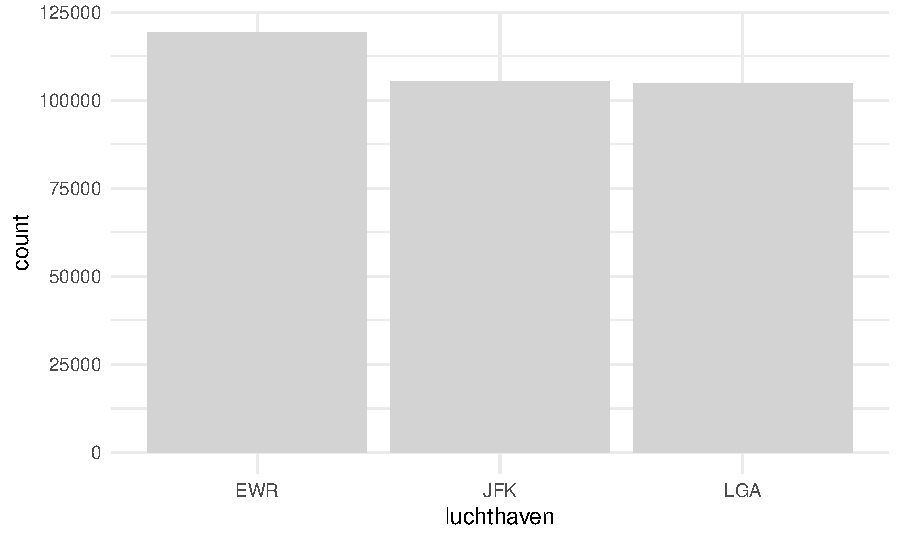
\includegraphics[width=1\linewidth]{textbook_files/figure-latex/2-3a-1} \caption[Staafdiagram luchthavens]{Staafdiagram luchthavens}\label{fig:2-3a}
\end{figure}

\begin{itemize}
\tightlist
\item
  Minder geschikt indien er veel waarden zijn. Dan wordt de X-as snel onleesbaar.(Fig. \ref{fig:2-3b})
\end{itemize}

\begin{figure}
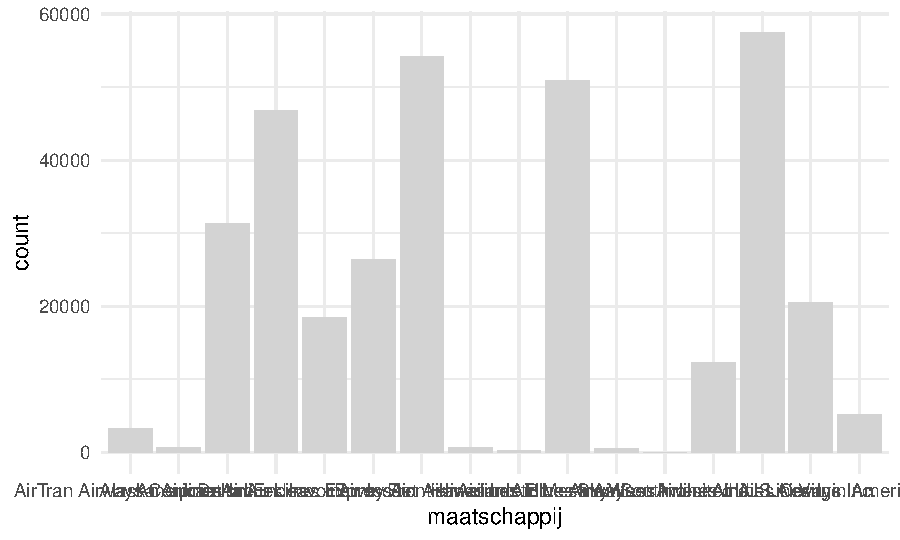
\includegraphics[width=1\linewidth]{textbook_files/figure-latex/2-3b-1} \caption[Staafdiagram maatschappijen]{Staafdiagram maatschappijen}\label{fig:2-3b}
\end{figure}

\begin{itemize}
\tightlist
\item
  Je kan natuurlijk de labels roteren. Maar dit kan nog steeds onhandig zijn om te lezen. (Fig. \ref{fig:2-3c}).
\end{itemize}

\begin{figure}
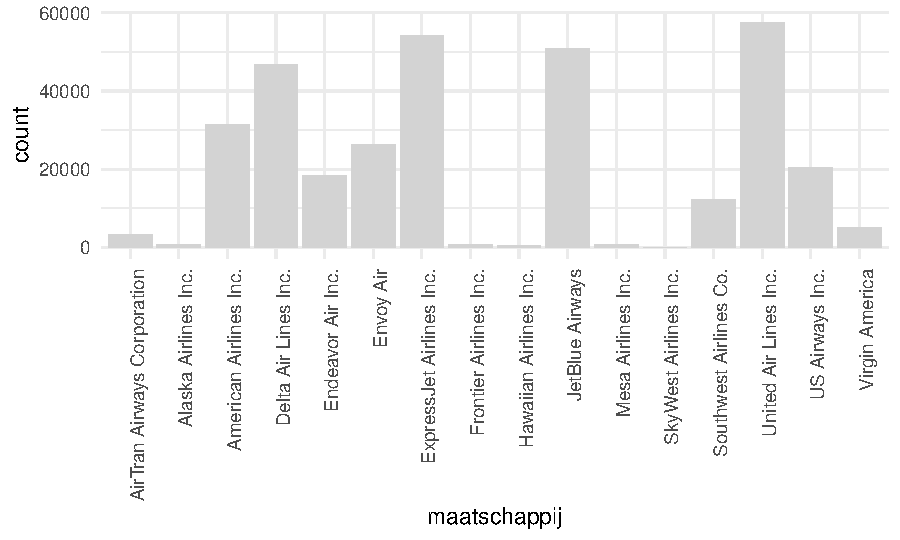
\includegraphics[width=1\linewidth]{textbook_files/figure-latex/2-3c-1} \caption[Staafdiagram met geroteerde labels]{Staafdiagram met geroteerde labels}\label{fig:2-3c}
\end{figure}

\begin{itemize}
\tightlist
\item
  In geval van een \textbf{nominale} variabele zijn er twee mogelijkheden om de waarden te rangschikken:

  \begin{itemize}
  \tightlist
  \item
    Alfabetisch. (standaard) Dit is handig om snel waarden terug te vinden.
  \item
    Volgens frequentie. Dit is handig om snel te zien welke waarden vaak/weinig voorkomen en geeft ook een beter beeld van de verdeling van de waarden. (Fig. \ref{fig:2-3d})
  \end{itemize}
\end{itemize}

\begin{figure}
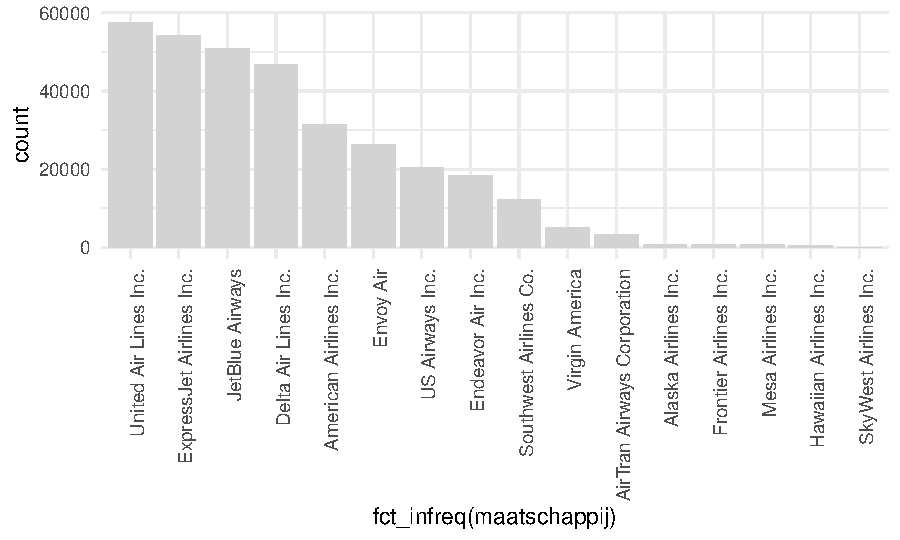
\includegraphics[width=1\linewidth]{textbook_files/figure-latex/2-3d-1} \caption[Staafdiagram gesorteerd op frequentie]{Staafdiagram gesorteerd op frequentie}\label{fig:2-3d}
\end{figure}

\begin{itemize}
\item
  In het geval van een \textbf{ordinale} variabele houd je best de intrinsieke volgorde van de waarden aan.
\item
  Je kan ook een horizontaal staafdiagram maken. (Fig. \ref{fig:2-3e})

  \begin{itemize}
  \tightlist
  \item
    Zelfde principe, maar dan met horizontale balken.
  \item
    Is handiger om de verschillende waarden te lezen, vooral indien dit er veel zijn.
  \end{itemize}
\end{itemize}

\begin{figure}
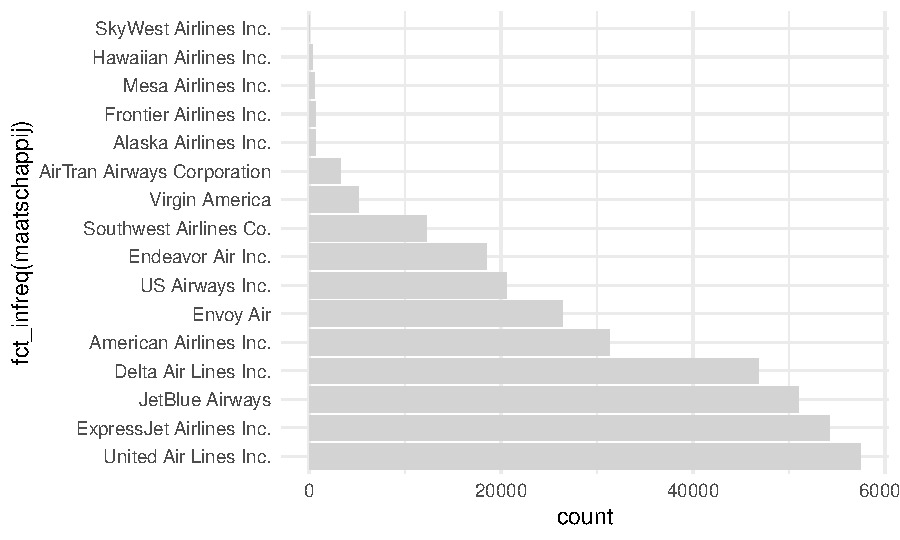
\includegraphics[width=1\linewidth]{textbook_files/figure-latex/2-3e-1} \caption[Verticaal staafdiagram gesorteerd op frequentie]{Verticaal staafdiagram gesorteerd op frequentie}\label{fig:2-3e}
\end{figure}

\hypertarget{dotplot}{%
\subsubsection{Dotplot}\label{dotplot}}

\begin{itemize}
\item
  In plaats van balken te gebruiken om de frequentie van een waarde aan te geven, kan je dit ook met punten doen. (Fig. \ref{fig:2-5a})
\item
  Een dotplot laat duidelijker zien waar de sprongen in de verdeling zit. Daarom is de dotplot vooral relevant als je de waarden ordent volgens frequentie.

  \begin{figure}
  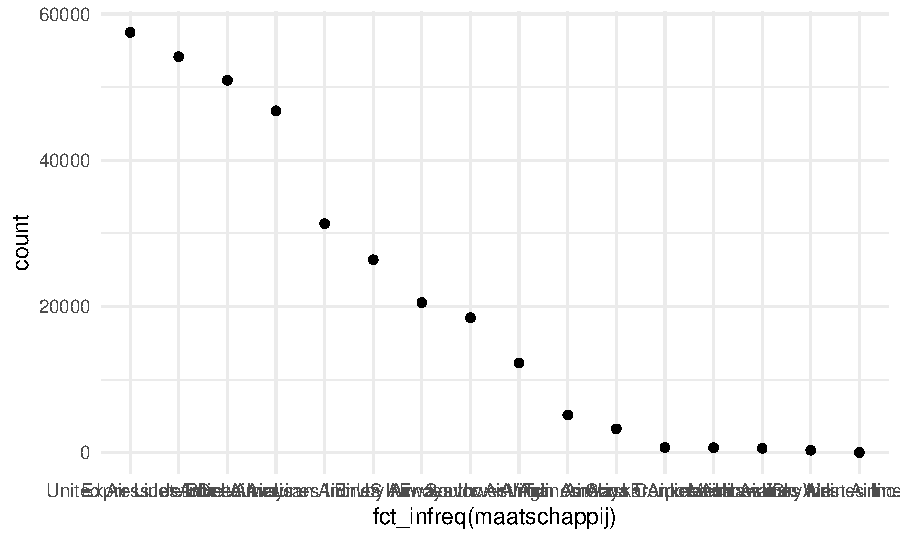
\includegraphics[width=1\linewidth]{textbook_files/figure-latex/2-5a-1} \caption[Dotplot maatschappij]{Dotplot maatschappij}\label{fig:2-5a}
  \end{figure}
\item
  Net als de barplot kan je zowel een verticale als horizontale dotplot maken. (Fig. \ref{fig:2-5b})
\end{itemize}

\begin{figure}
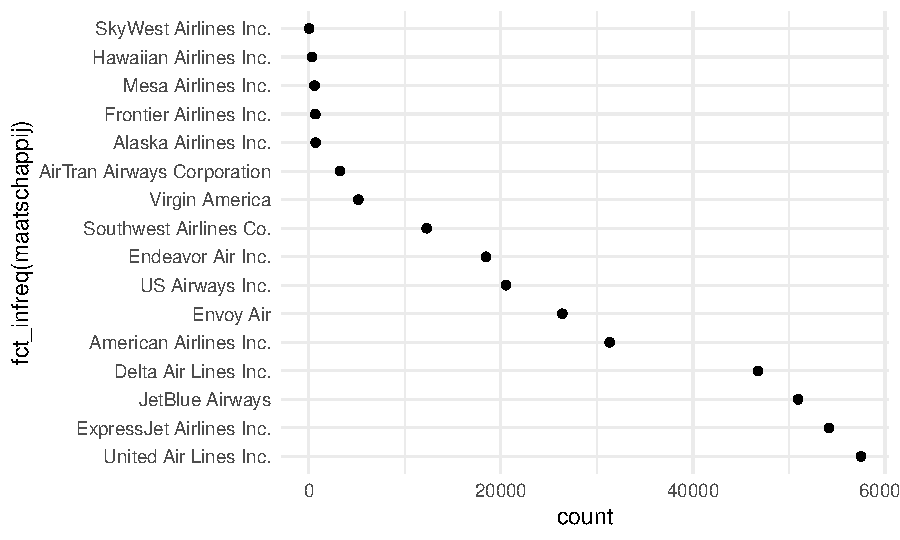
\includegraphics[width=1\linewidth]{textbook_files/figure-latex/2-5b-1} \caption[Verticale dotplot]{Verticale dotplot}\label{fig:2-5b}
\end{figure}

\hypertarget{stacked-staafdiagram}{%
\subsubsection{`Stacked' staafdiagram}\label{stacked-staafdiagram}}

\begin{itemize}
\tightlist
\item
  We maken nu slechts 1 kolom. Iedere waarde is een andere kleur en neemt een deel van de balk in beslag. De volledige balk stelt 100\% van de data voor. (Fig. \ref{fig:2-6a})
\item
  Kan nuttig zijn om data cumulatief te bestuderen.
\item
  Hiermee kunnen we vragen beantwoorden zoals: ``Welke waarden moeten we nemen om met zo weinig mogelijk waarden x\% van de objecten te hebben?''
\end{itemize}

\begin{figure}

{\centering 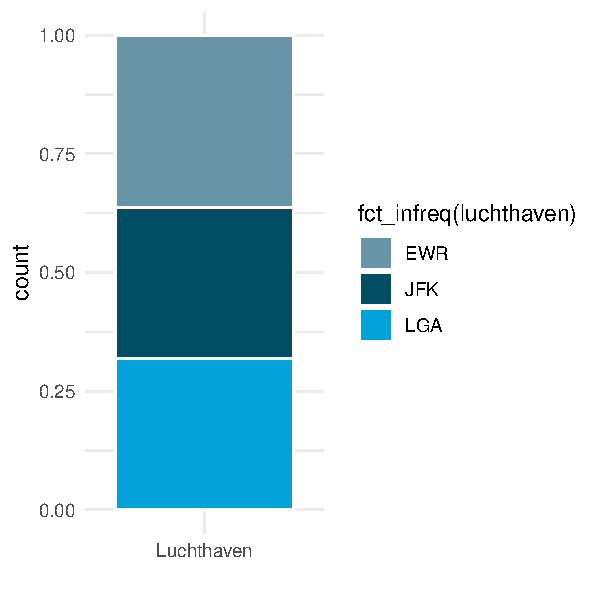
\includegraphics[width=0.7\linewidth]{textbook_files/figure-latex/2-6a-1} 

}

\caption[Stacked barplot]{Stacked barplot}\label{fig:2-6a}
\end{figure}

\begin{itemize}
\tightlist
\item
  We kunnen ook horizontale versies maken. (Fig. \ref{fig:2-6b})
\end{itemize}

\begin{figure}
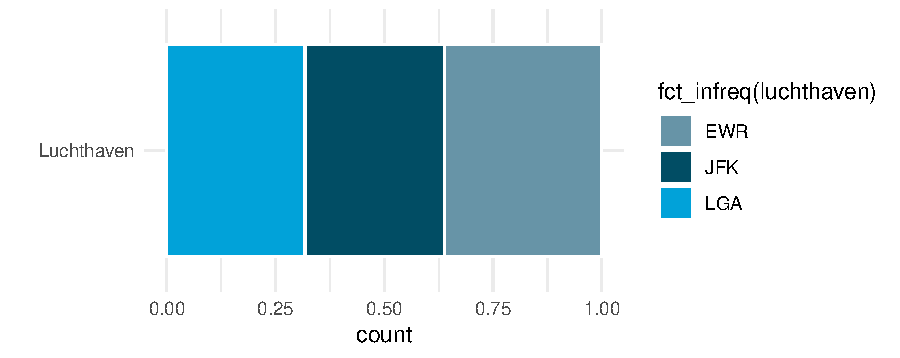
\includegraphics[width=1\linewidth]{textbook_files/figure-latex/2-6b-1} \caption[Horizontale stacked barplot]{Horizontale stacked barplot}\label{fig:2-6b}
\end{figure}

\begin{itemize}
\tightlist
\item
  Univariate stacked barcharts kunnen soms wat \emph{raar} overkomen. Vaak komt een gewone barchart beter over.
\end{itemize}

\hypertarget{andere-soorten}{%
\subsubsection{Andere soorten}\label{andere-soorten}}

\begin{itemize}
\tightlist
\item
  treemap: indelen van rechthoekige oppervlakte volgens categorische variabelen
\item
  pie chart

  \begin{itemize}
  \tightlist
  \item
    Moeilijk te interpreteren.
  \item
    Verschillen tussen waarden zijn enkel duidelijk bij grote verschillen, terwijl barplots en dotplots deze ook bij kleine verschillen kunnen tonen.
  \item
    Voor cumulatieve analyses van de data zijn barplots beter omdat het hier eenvoudiger is om af te leiden waar x\% zicht bevindt.
  \end{itemize}
\end{itemize}

\hypertarget{continue-variabele}{%
\subsection{Continue variabele}\label{continue-variabele}}

\hypertarget{histogram}{%
\subsubsection{Histogram}\label{histogram}}

\begin{itemize}
\tightlist
\item
  Analoog met barplot, alleen gaan we hier eerst onze ``categorieën'' definiëren. (Fig. \ref{fig:2-7a})
\item
  Dit wordt `binning' genoemd en wordt bepaald door een bin-breedte te kiezen.
\item
  Je kan de binbreedte rechtstreeks kiezen of bepalen door vast te leggen hoeveel categorieën/bins je wenst.
\end{itemize}

\begin{figure}
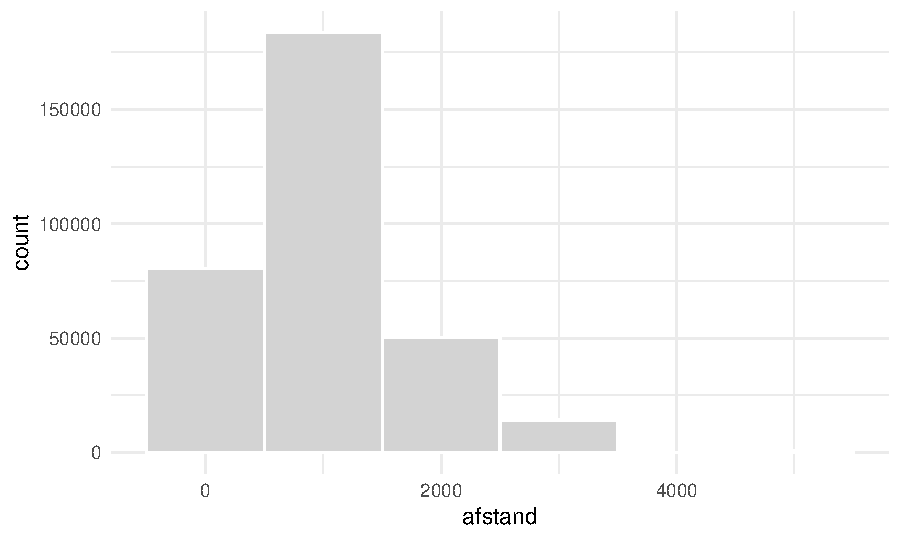
\includegraphics[width=1\linewidth]{textbook_files/figure-latex/2-7a-1} \caption[Histogram with binwidth 1000]{Histogram with binwidth 1000}\label{fig:2-7a}
\end{figure}

\begin{itemize}
\tightlist
\item
  Voor de visualisatie, worden alle waarden gegroepeerd per `bin'.
\item
  De binbreedte kan een enorme impact hebben op het uitzicht van de verdeling. (Fig. \ref{fig:2-7b} - \ref{fig:2-7c})

  \begin{itemize}
  \tightlist
  \item
    Hoe breder de bins, hoe minder modi je kan detecteren.
  \item
    Hoe smaller de bins, hoe meer modi je gaat zien, hoewel dit niet altijd even betekenisvol is.
  \item
    Hoe smaller de bins, hoe minder data er in iedere bin gaat zitten en dan kunnen patronen wel in jouw dataset bestaan maar louter ten gevolge van toeval.
  \end{itemize}
\end{itemize}

\begin{figure}
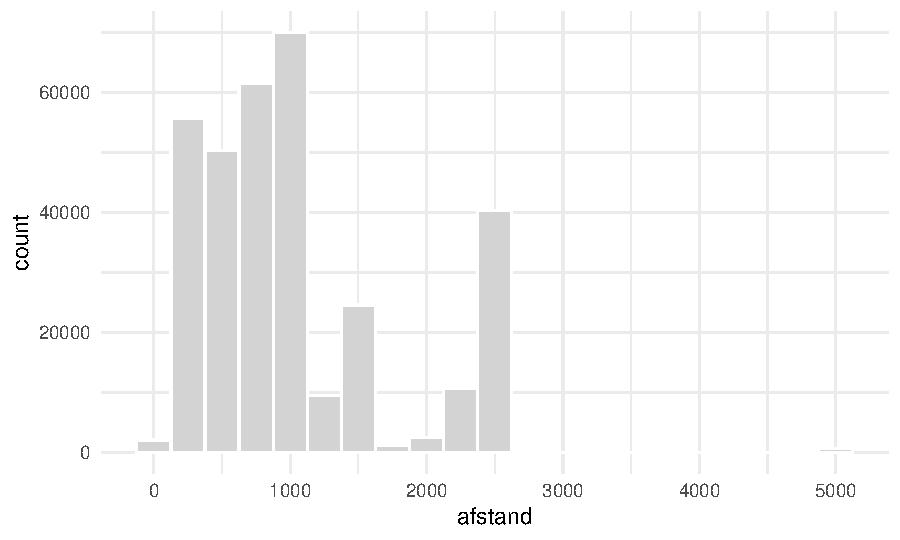
\includegraphics[width=1\linewidth]{textbook_files/figure-latex/2-7b-1} \caption[Histogram with binwidth 250]{Histogram with binwidth 250}\label{fig:2-7b}
\end{figure}

\begin{figure}
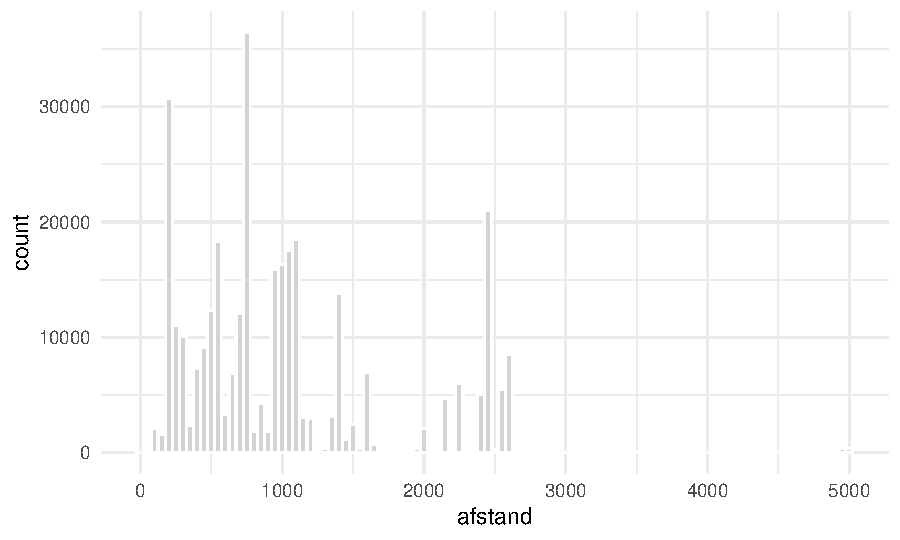
\includegraphics[width=1\linewidth]{textbook_files/figure-latex/2-7c-1} \caption[Histogram with binwidth 50]{Histogram with binwidth 50}\label{fig:2-7c}
\end{figure}

\hypertarget{density}{%
\subsubsection{Density}\label{density}}

\begin{itemize}
\tightlist
\item
  Variant van histogram.
\item
  In plaats van staven wordt er een curve getekend. (Fig. \ref{fig:2-density})
\item
  De oppervlakte onder de curve is steeds gelijk aan 1
\item
  Hoe hoger de curve, hoe meer observaties ter hoogt van deze waarde (hoe hoger de densiteit)
\item
  De waarde van de y-as heeft geen directe betekenis.
\end{itemize}

\begin{figure}
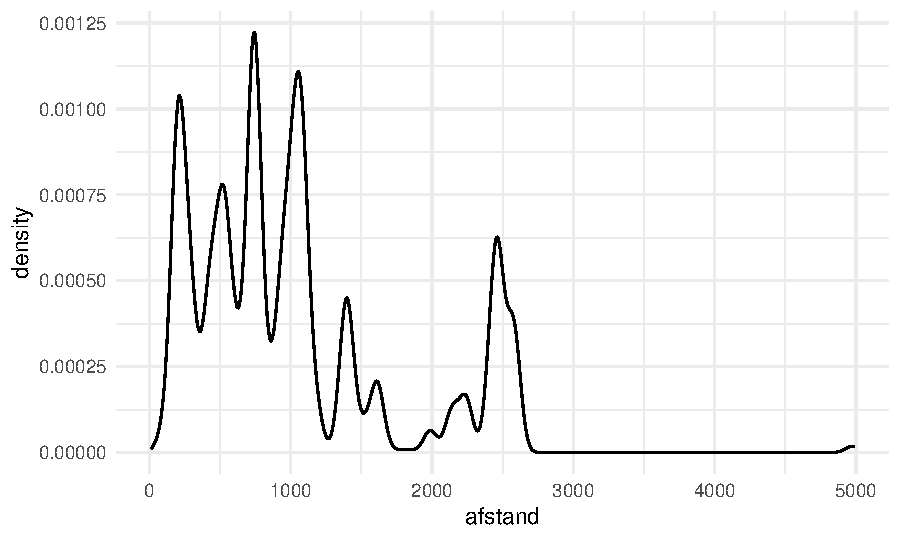
\includegraphics[width=1\linewidth]{textbook_files/figure-latex/2-density-1} \caption[Density plot]{Density plot}\label{fig:2-density}
\end{figure}

\hypertarget{boxplot}{%
\subsubsection{Boxplot}\label{boxplot}}

\begin{itemize}
\tightlist
\item
  De lijn in het midden duidt de mediaan aan. Dit betekent dat 50\% van je data onder deze lijn ligt, terwijl 50\% er boven ligt. (Fig. \ref{fig:2-8})
\item
  De box in het midden duidt de middelste 50\% van je data aan. Dit wordt ook de interkwartiel-box genoemd. Dit betekent dat 25\% van je data onder deze box zit en nog eens 25\% boven deze box ligt. Hoe groter de box, des te meer de data gespreid is.
\item
  Indien de box aan één zijde van de mediaanlijn groter is dan aan de andere zijde, dan wijst dit er op dat de data meer gespreid is aan die kant.
\item
  De ``whiskers'' geven de laatste datapunten aan die als ``normaal'' beschouwd worden. Datapunten buiten deze grenzen beschouwt een boxplot als outliers of extreme waarden.
\item
  De grens waar data van normaal naar extreem overgaat wordt door de boxplot bepaald door anderhalf keer de grootte van de interkwartiel-box op te tellen (en af te trekken) van de bovenste (onderste) grens van de interkwartiel-box. Punten die hier buiten liggen zijn outliers en worden als aparte punten aangeduid. De uitersten van de whiskers duiden de laatste datapunten aan binnen deze grenzen.
\end{itemize}

\begin{figure}

{\centering 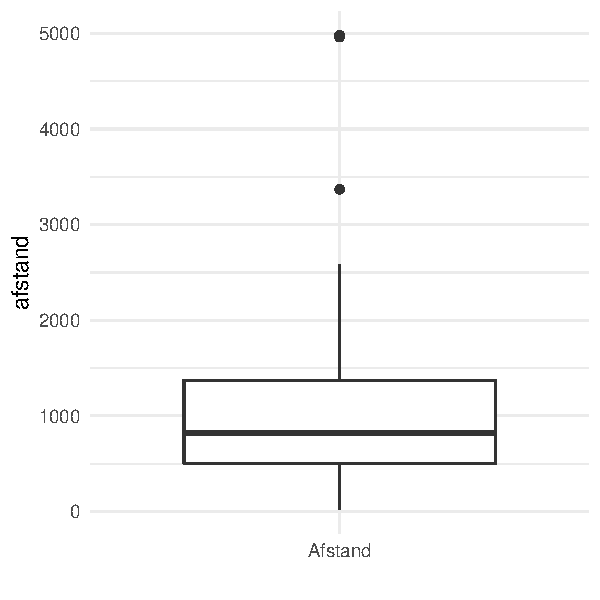
\includegraphics[width=0.7\linewidth]{textbook_files/figure-latex/2-8-1} 

}

\caption[Verticale boxplot vertrekvertraging]{Verticale boxplot vertrekvertraging}\label{fig:2-8}
\end{figure}

\begin{itemize}
\tightlist
\item
  Het is niet abnormaal dat er outliers in je data aanwezig zijn.
\item
  Bij normaal verdeelde data zal je gemiddeld 7 outliers per 1000 datapunten mogen verwachten.

  \begin{itemize}
  \tightlist
  \item
    Een normale verdeling is een bepaalde manier waarop data waarden verdeeld kunnen zijn die in de realiteit vaak voorkomt.
  \end{itemize}
\item
  Indien je echter veel meer outliers ziet op je boxplot visualisatie, dan is de kans reëel dat er meer aan de hand is:

  \begin{itemize}
  \tightlist
  \item
    Er zijn bijvoorbeeld systematische meetfouten
  \item
    De objecten in je data zijn in feite op bepaalde aspecten significant verschillend waardoor je ze apart zou moeten bestuderen.
  \end{itemize}
\item
  Je kan een boxplot ook roteren. (Fig \ref{fig:2-9})
\item
  Boxplots komen beter tot hun recht bij bivariate analyses dan bij univariate analyses.
\end{itemize}

\begin{figure}
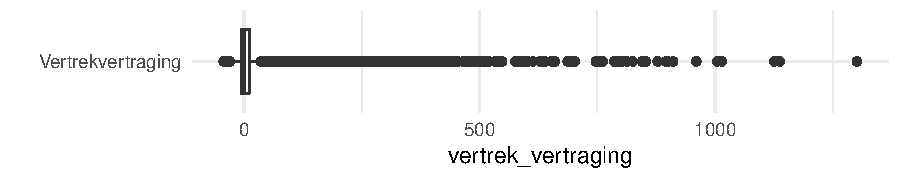
\includegraphics[width=1\linewidth]{textbook_files/figure-latex/2-9-1} \caption[Horizontale boxplot vertrekvertraging]{Horizontale boxplot vertrekvertraging}\label{fig:2-9}
\end{figure}

\hypertarget{violin-plot}{%
\subsubsection{Violin plot}\label{violin-plot}}

\begin{itemize}
\tightlist
\item
  Een violin plot kan je beschouwen als een combinatie van een histogram en een boxplot. (Fig. @ref(fig:2\_10a))
\item
  Net als bij een boxplot wordt op verticale wijze getoond hoe de data verspreid is.
\item
  Opnieuw kan je ervoor kiezen de grafiek te roteren. (Fig. @ref(fig:2\_10b))
\item
  Net als bij een histogram kan je goed zien waar het volume (de massa) van de data zich bevindt.
\item
  Net als bij een histogram kan je detecteren hoeveel modi de data bezit.
\item
  In tegenstelling tot de boxplot, kan je bij een violinplot wel niet duidelijk zien waar bijvoorbeeld het `midden' van je data is.
\end{itemize}

\begin{figure}

{\centering 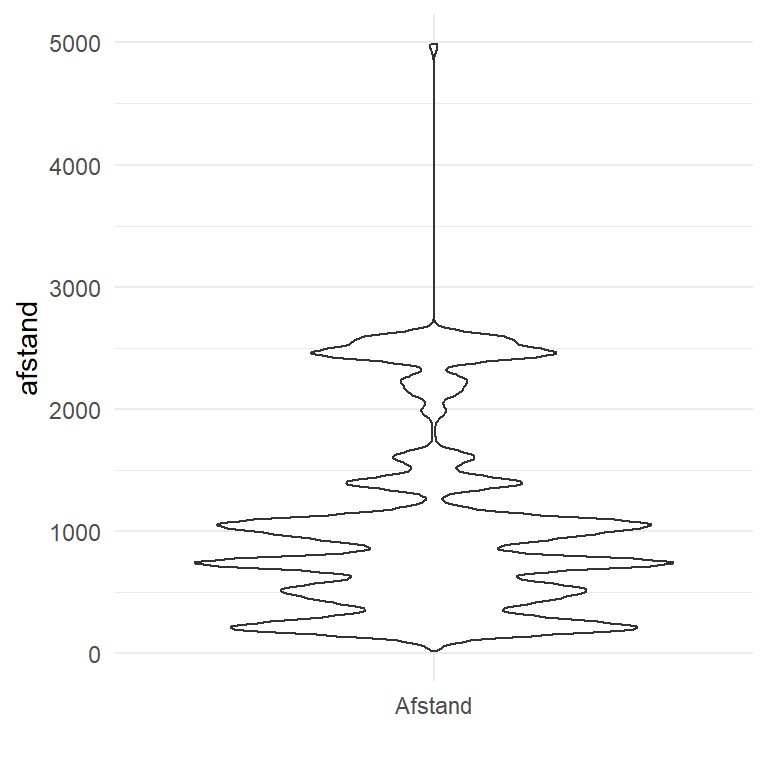
\includegraphics[width=0.7\linewidth]{textbook_files/figure-latex/2-10a-1} 

}

\caption[Verticale violin plot afstand]{Verticale violin plot afstand}\label{fig:2-10a}
\end{figure}

\begin{figure}
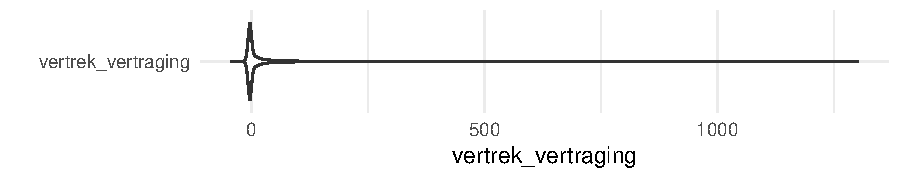
\includegraphics[width=1\linewidth]{textbook_files/figure-latex/2-10b-1} \caption[Horizontale violin plot vertrekvertraging]{Horizontale violin plot vertrekvertraging}\label{fig:2-10b}
\end{figure}

\hypertarget{jitter-plot}{%
\subsubsection{Jitter plot}\label{jitter-plot}}

\begin{itemize}
\tightlist
\item
  puntenwolk waarbij willekeurige ``noise'' (ruis) wordt toegevoegd.
\item
  de ruis zorgt ervoor dat datapunten niet overlappen, en dat het duidelijk is waar de massa zich bevindt.
\item
  Fig. \ref{fig:2-jitter} toont een vergelijking van violin, boxplot, point en jitter plot.
\end{itemize}

\begin{figure}
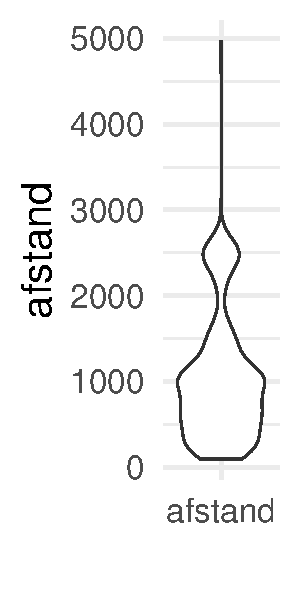
\includegraphics[width=0.24\linewidth]{textbook_files/figure-latex/2-jitter-1} 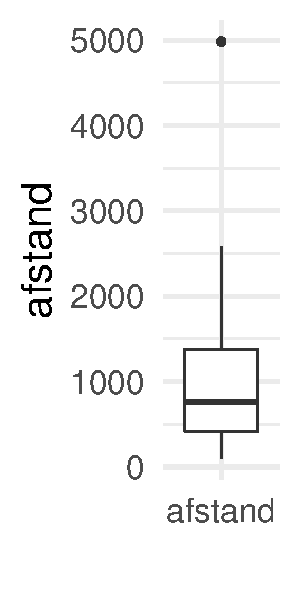
\includegraphics[width=0.24\linewidth]{textbook_files/figure-latex/2-jitter-2} 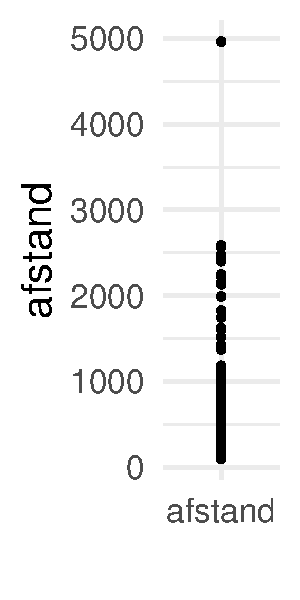
\includegraphics[width=0.24\linewidth]{textbook_files/figure-latex/2-jitter-3} 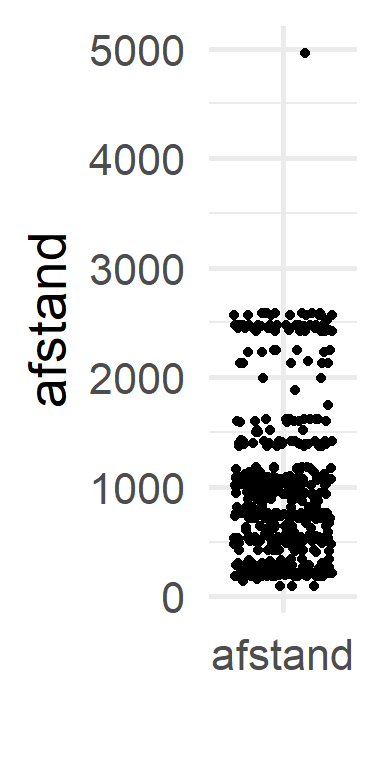
\includegraphics[width=0.24\linewidth]{textbook_files/figure-latex/2-jitter-4} \caption[Violin, boxplot, point en jitter]{Violin, boxplot, point en jitter}\label{fig:2-jitter}
\end{figure}

\hypertarget{bivariate-visualisatie-2-variabelen}{%
\section{Bivariate visualisatie (2 variabelen)}\label{bivariate-visualisatie-2-variabelen}}

\begin{itemize}
\tightlist
\item
  Wanneer we de relatie tussen 2 variabelen bekijken is het eenvoudig te denken in \emph{oorzaak} en gevolg \emph{termen.} \footnote{Zie opmerking i.v.m. correlatie versus causaliteit, \ref{how-charts-lie}.}

  \begin{itemize}
  \tightlist
  \item
    De variabele die we het label ``oorzaak'' geven, zullen we voortaan ``onafhankelijke variabele'' noemen.
  \item
    De variabele die we het label ``gevolg'' geven, zullen we voortaan ``afhankelijke variabele'' noemen.
  \end{itemize}
\item
  Waar we eigenlijk in geïnteresseerd zijn bij een visualisatie van 2 variabelen is de impact van de onafhankelijke variabele op de afhankelijke variabele weer te geven.
\item
  Alle vragen die we kunnen stellen bij de visualisatie van één variabele, kunnen we nog steeds stellen, met telkens de bijkomende vraag of het waargenomen patroon verandert als de onafhankelijke variabele van waarde verandert.
\end{itemize}

\hypertarget{situatie-1-de-onafhankelijke-variabele-is-categorisch}{%
\subsection{Situatie 1: De onafhankelijke variabele is categorisch}\label{situatie-1-de-onafhankelijke-variabele-is-categorisch}}

Indien de afhankelijke variabele een continue variabele is kan je:

\begin{itemize}
\tightlist
\item
  meerdere boxplots op 1 grafiek visualiseren, met telkens 1 boxplot per waarde van de onafhankelijke variabele. (Fig. \ref{fig:2-12a})
\end{itemize}

\begin{figure}
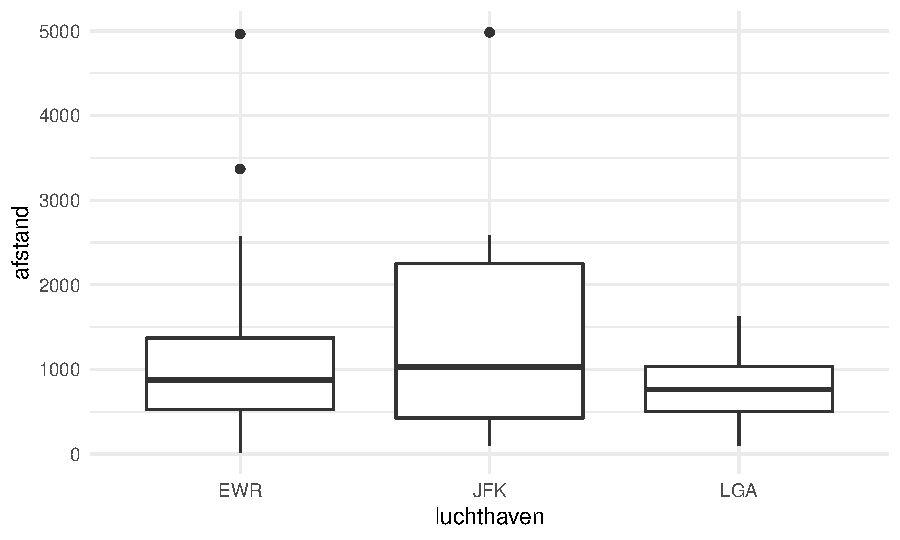
\includegraphics[width=1\linewidth]{textbook_files/figure-latex/2-12a-1} \caption[Bivariate boxplot]{Bivariate boxplot}\label{fig:2-12a}
\end{figure}

\begin{itemize}
\tightlist
\item
  meerdere violinplots op 1 grafiek tonen, met telkens 1 violinplot per waarde van de onafhankelijke variabele. (Fig. \ref{fig:2-12b})
\end{itemize}

\begin{figure}
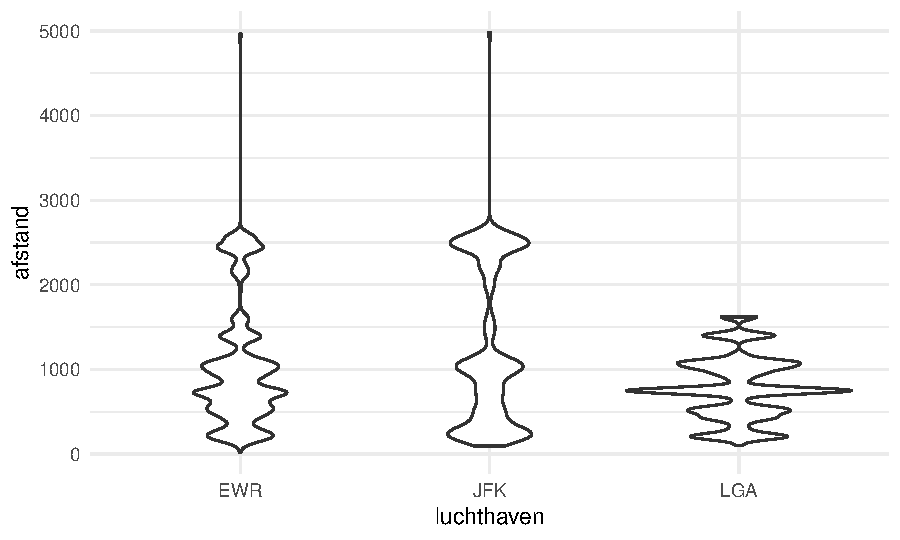
\includegraphics[width=1\linewidth]{textbook_files/figure-latex/2-12b-1} \caption[Bivariate violin plot]{Bivariate violin plot}\label{fig:2-12b}
\end{figure}

\begin{itemize}
\tightlist
\item
  meerdere histogrammen op 1 grafiek tonen

  \begin{itemize}
  \tightlist
  \item
    Hiervoor gebruiken we facetten: we tekenen voor elke waarde van de onafhankelijke variabele een apart assenstelsel. (Fig. \ref{fig:2-12c})
  \end{itemize}
\end{itemize}

\begin{figure}
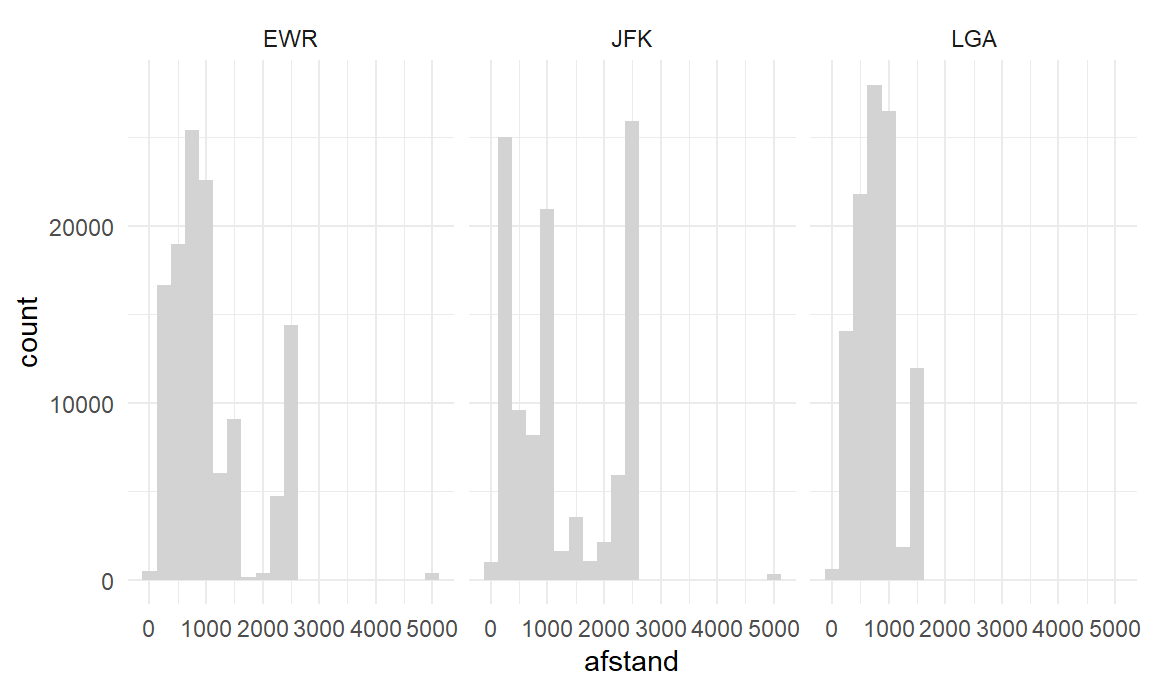
\includegraphics[width=1\linewidth]{textbook_files/figure-latex/2-12c-1} \caption[Bivariate histogram plot]{Bivariate histogram plot}\label{fig:2-12c}
\end{figure}

\begin{itemize}
\tightlist
\item
  meerdere density plots
\item
  Hiervoor kunnen we facetten gebruiken, ofwel de density plots over elkaar tekenen en onderscheiden met kleur. (Fig. \ref{fig:2-12d}-\ref{fig:2-12e})
\end{itemize}

\begin{figure}
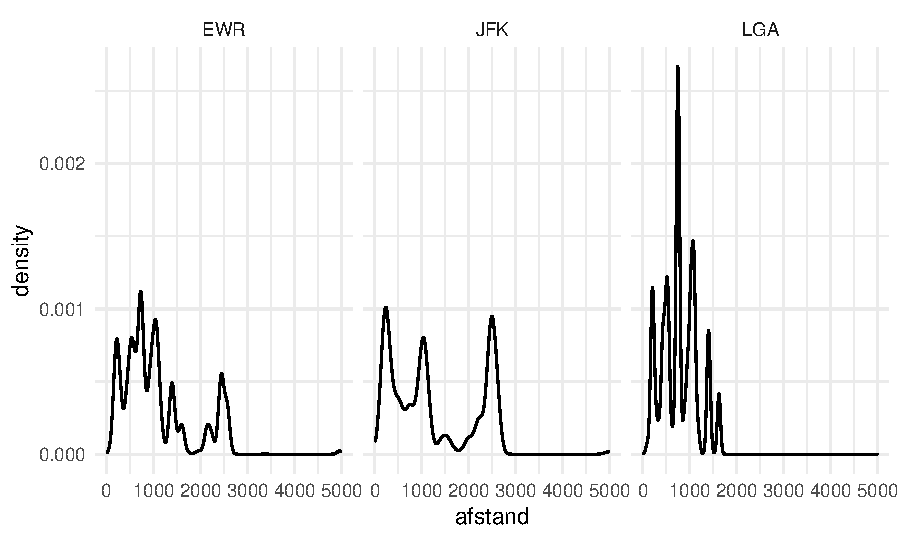
\includegraphics[width=1\linewidth]{textbook_files/figure-latex/2-12d-1} \caption[Bivariate density plot - apart]{Bivariate density plot - apart}\label{fig:2-12d}
\end{figure}

\begin{figure}
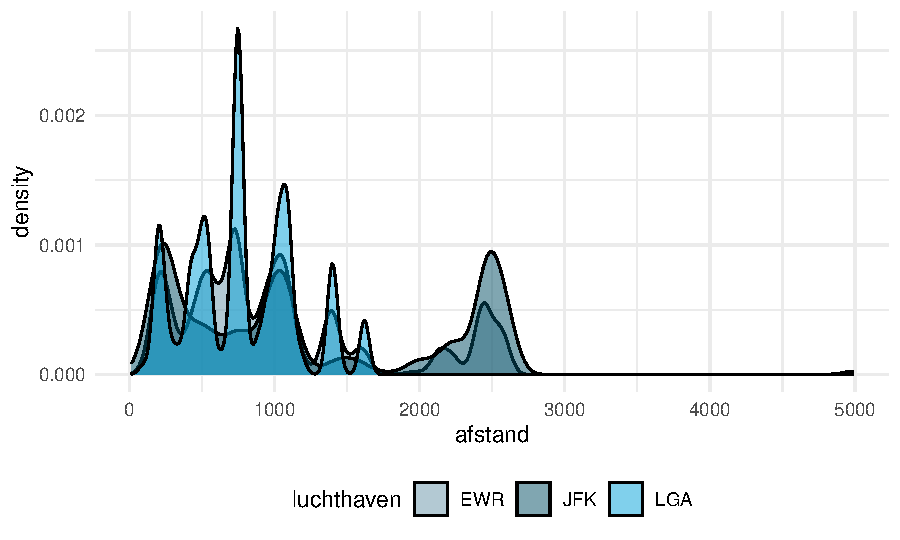
\includegraphics[width=1\linewidth]{textbook_files/figure-latex/2-12e-1} 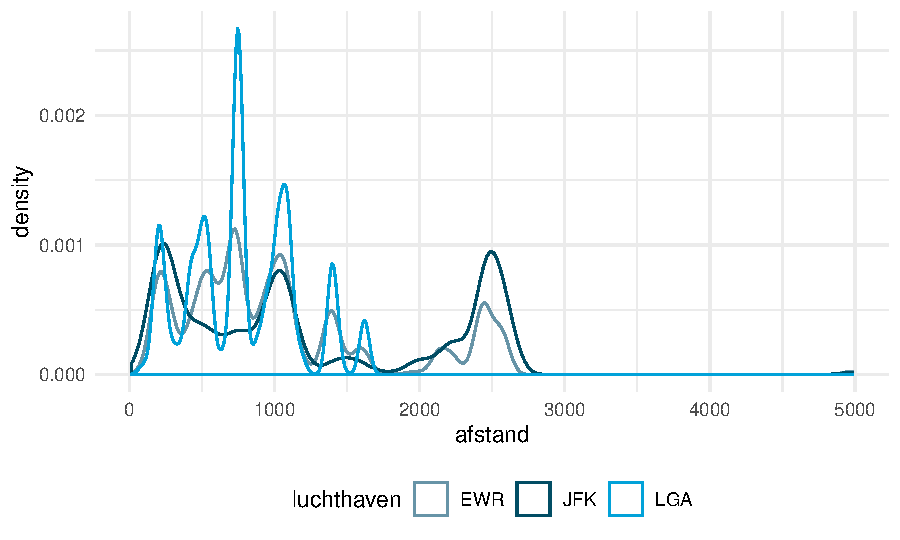
\includegraphics[width=1\linewidth]{textbook_files/figure-latex/2-12e-2} \caption[Bivariate density plot - overlappend]{Bivariate density plot - overlappend}\label{fig:2-12e}
\end{figure}

Indien de afhankelijke variabele een \textbf{categorische variabele} is:

\begin{itemize}
\tightlist
\item
  Kan je meerdere barplots op 1 grafiek visualiseren, met telkens de bars gegroepeerd per waarde van de onafhankelijke variabele.
\end{itemize}

\begin{figure}
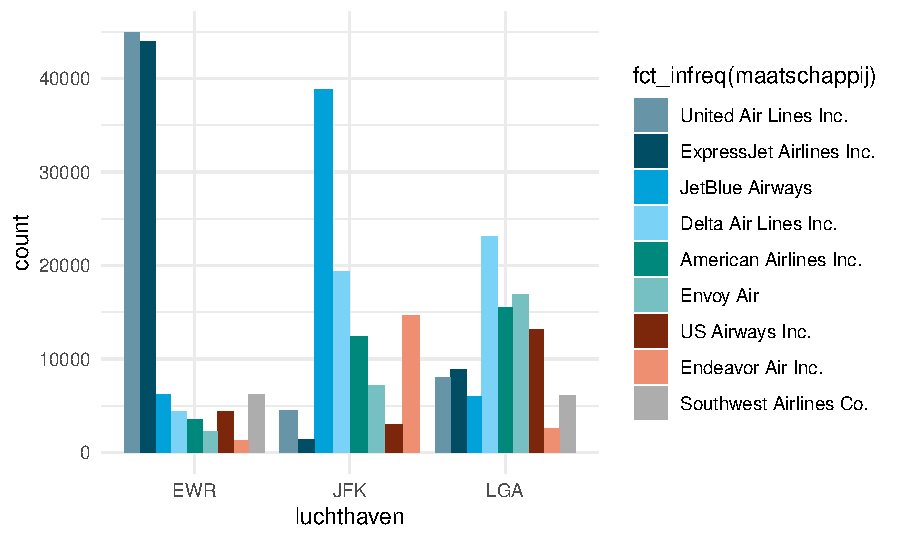
\includegraphics[width=1\linewidth]{textbook_files/figure-latex/2-13a-1} \caption[Bivariate barplot]{Bivariate barplot}\label{fig:2-13a}
\end{figure}

\begin{itemize}
\tightlist
\item
  Kan je meerdere stacked barplots op 1 grafiek plaatsen, met telkens een volledige stack per waarde van de onafhankelijke variabele.
\end{itemize}

\begin{figure}
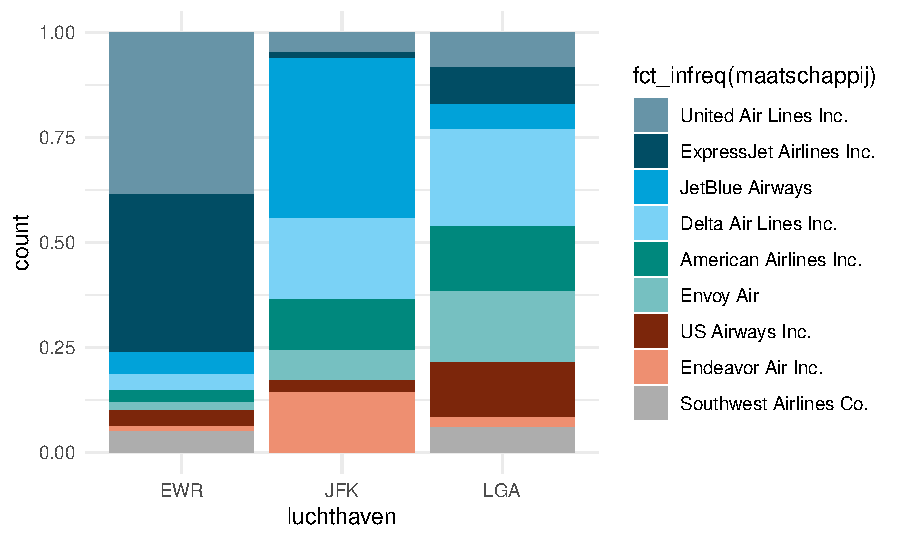
\includegraphics[width=1\linewidth]{textbook_files/figure-latex/2-13b-1} \caption[Bivariate stacked barplot]{Bivariate stacked barplot}\label{fig:2-13b}
\end{figure}

\begin{itemize}
\tightlist
\item
  Kan je een heatmap (of tile plot) gebruiken. Hier bij plaats je 2 categorische variabelen op de x-as en y-as, respectivelijk.

  \begin{itemize}
  \tightlist
  \item
    Voor elke combinatie van waarden is er een tegel die je kan inkleuren volgens de frequentie van de combinatie.
  \end{itemize}
\end{itemize}

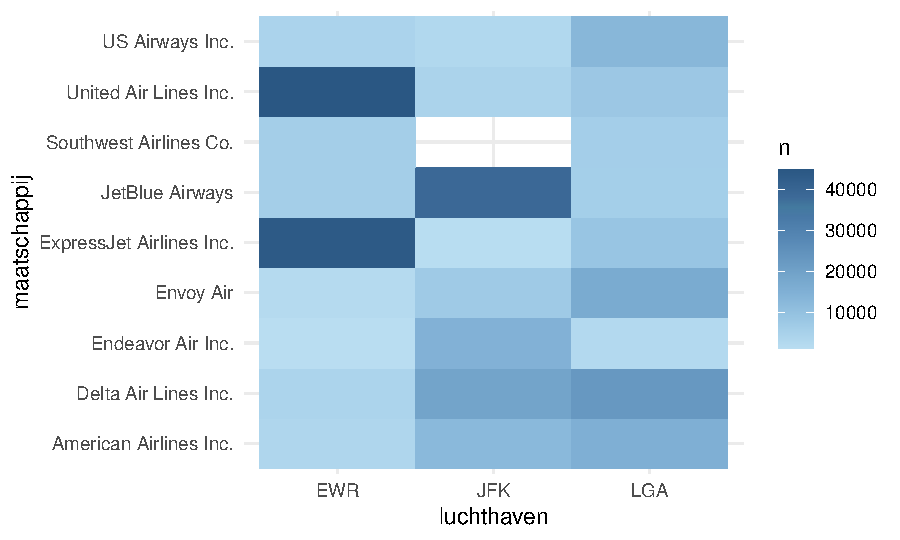
\includegraphics[width=1\linewidth]{textbook_files/figure-latex/unnamed-chunk-7-1}

\begin{itemize}
\tightlist
\item
  Je kan bijkomende ook de exacte waarde in elke tegel plotten.
\end{itemize}

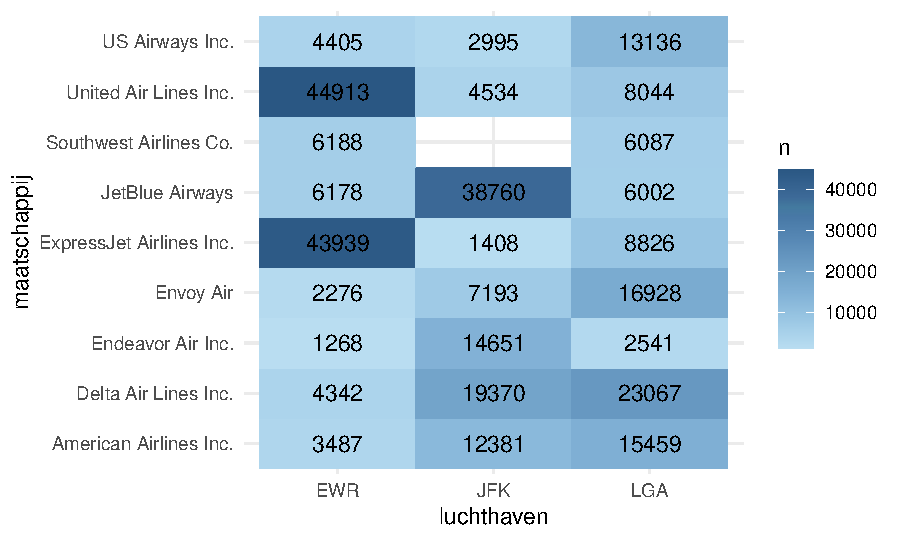
\includegraphics[width=1\linewidth]{textbook_files/figure-latex/unnamed-chunk-8-1}

\textbf{Let op} wanneer beide variabelen categorisch zijn, is het nog steeds van belang welke je beschouwd als afhankelijke en welke als onafhankelijke. Technisch kan je ze omdraaien, maar de betekenis van je visualizatie is niet dezelfde!

\begin{figure}
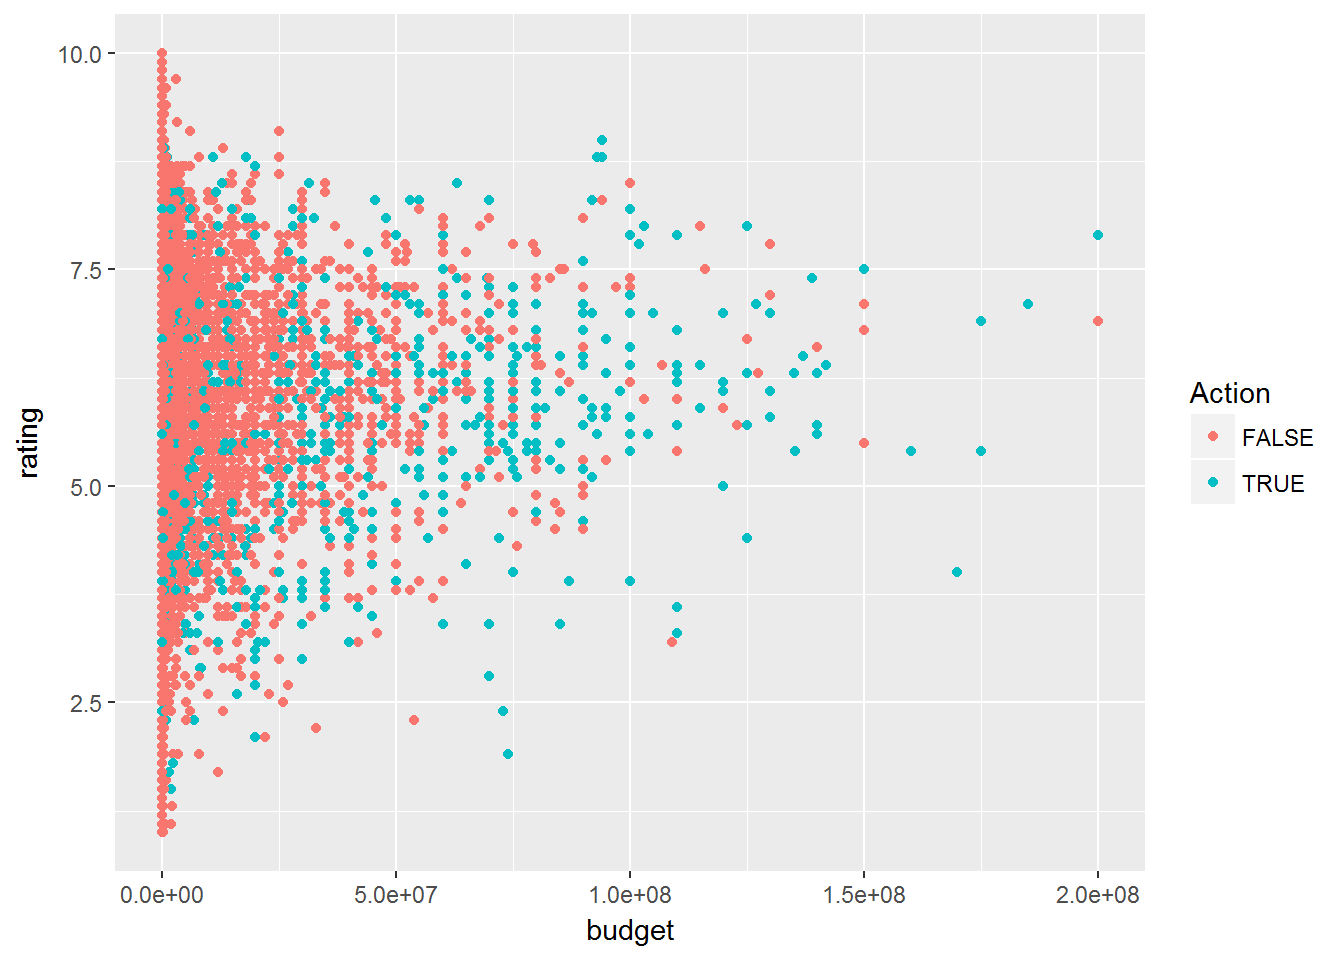
\includegraphics[width=1\linewidth]{textbook_files/figure-latex/unnamed-chunk-9-1} 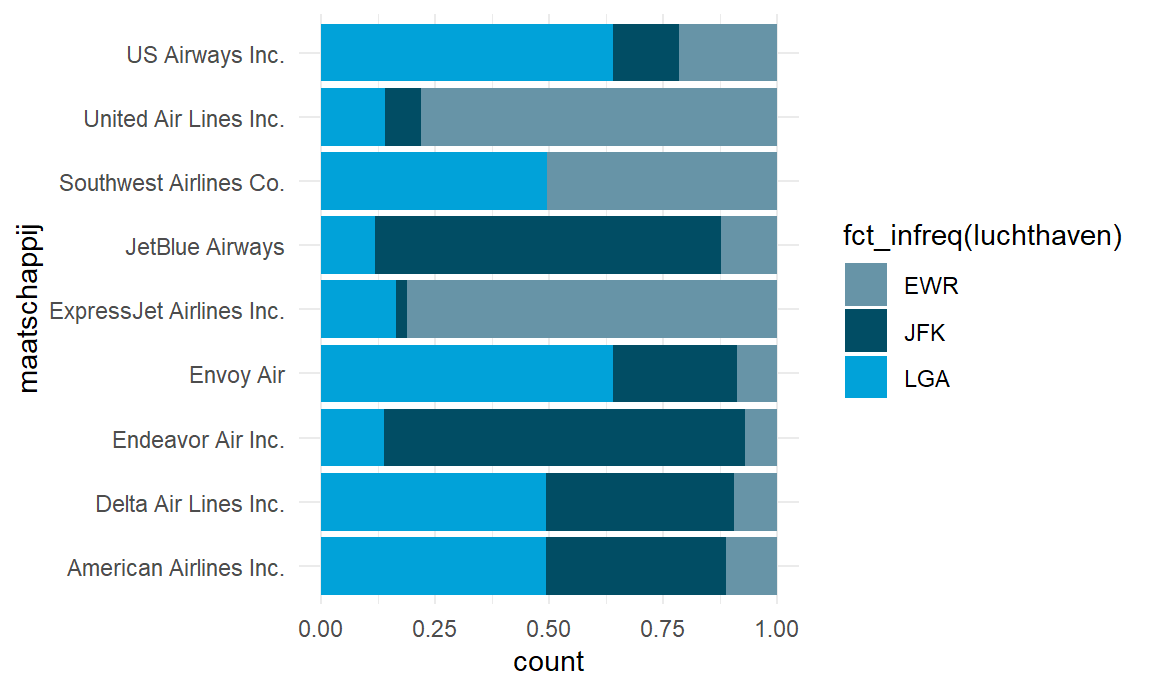
\includegraphics[width=1\linewidth]{textbook_files/figure-latex/unnamed-chunk-9-2} \caption[Twee verschillende stacked barcharts van luchthaven en maatschappij]{Twee verschillende stacked barcharts van luchthaven en maatschappij.}\label{fig:unnamed-chunk-9}
\end{figure}

Andere mogelijkheden:

\begin{itemize}
\tightlist
\item
  treemap (Fig. \ref{fig:treemap})
\end{itemize}

\begin{figure}
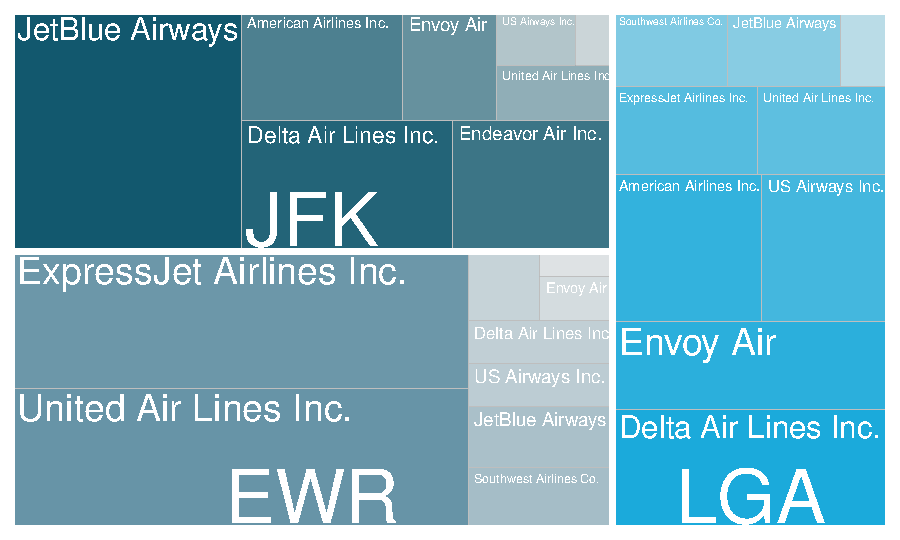
\includegraphics[width=1\linewidth]{textbook_files/figure-latex/treemap-1} \caption[Treemap luchthaven en maatschappij]{Treemap luchthaven en maatschappij.}\label{fig:treemap}
\end{figure}

\begin{itemize}
\tightlist
\item
  mosaic plot (Fig. \ref{fig:mosaic})
\end{itemize}

\begin{figure}
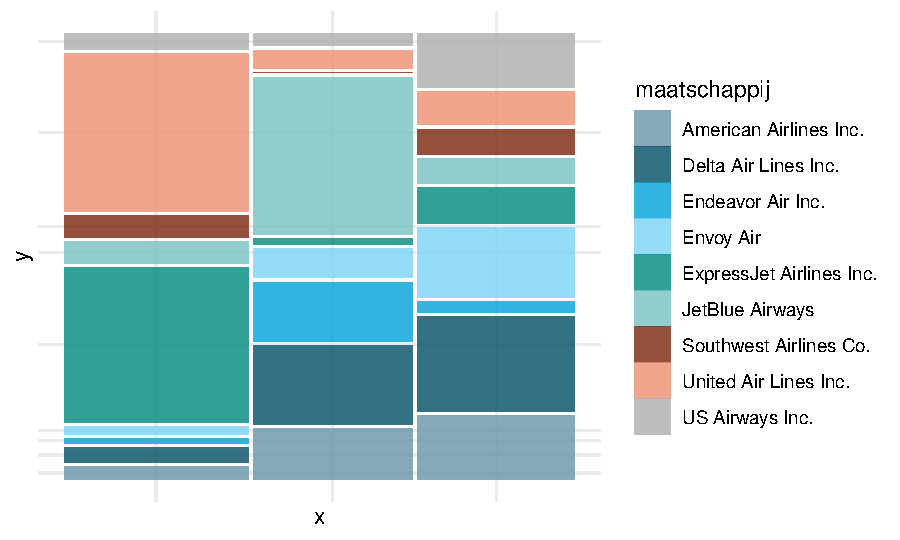
\includegraphics[width=1\linewidth]{textbook_files/figure-latex/mosaic-1} \caption[Mosaic plot luchthaven en maatschappij]{Mosaic plot luchthaven en maatschappij.}\label{fig:mosaic}
\end{figure}

\hypertarget{situatie-2-de-onafhankelijke-variabele-is-continue}{%
\subsection{Situatie 2: De onafhankelijke variabele is continue}\label{situatie-2-de-onafhankelijke-variabele-is-continue}}

\textbf{In dit geval kan je geen aparte plot per mogelijke waarde van de onafhankelijke variabele maken omdat er mogelijk oneindig veel waarden zijn.}

Indien de afhankelijke variabele continu is, dan kan je een scatterplot maken.

\begin{itemize}
\tightlist
\item
  Iedere observatie is een punt in je grafiek, waarbij de x-waarde op de grafiek overeenkomt met de waarde van de onafhankelijke variabele en de y-waarde op de grafiek overeenkomt met de waarde van de afhankelijke variabele.
\end{itemize}

\begin{figure}
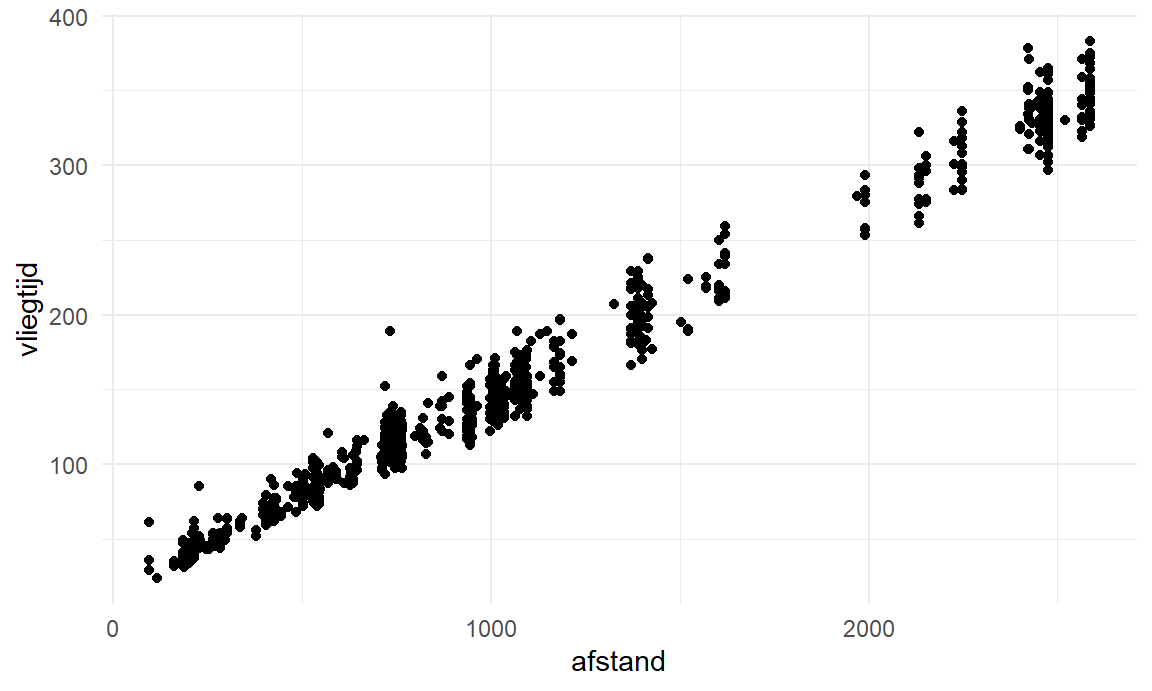
\includegraphics[width=1\linewidth]{textbook_files/figure-latex/213c-1} \caption[Scatterplot]{Scatterplot}\label{fig:213c}
\end{figure}

\begin{itemize}
\tightlist
\item
  Om patronen beter te herkennen kan je een ``trend-lijn'' toevoegen.
\end{itemize}

\begin{figure}
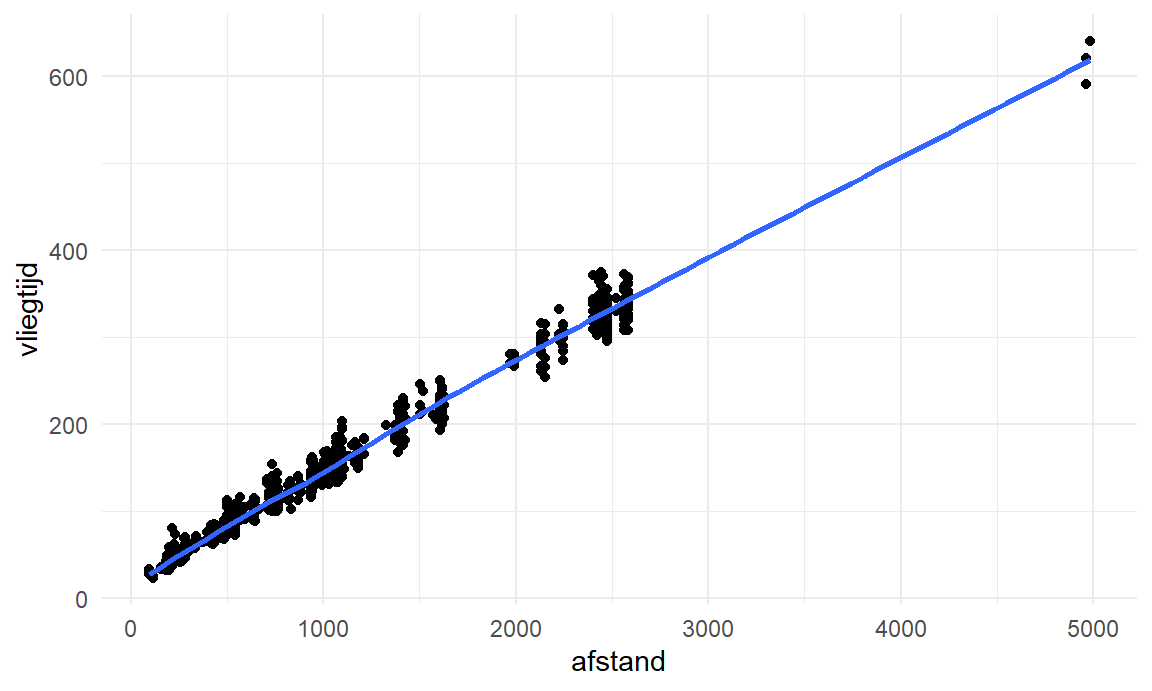
\includegraphics[width=1\linewidth]{textbook_files/figure-latex/2-13d-1} \caption[Scatterplot met trendlijn]{Scatterplot met trendlijn}\label{fig:2-13d}
\end{figure}

\begin{itemize}
\tightlist
\item
  Bij scatterplots is er gevaar voor overplotting
\item
  Mogelijke oplossingen

  \begin{itemize}
  \tightlist
  \item
    2D histogram: verdeel veld op in vierkante bins en tel per bin hoeveel data punten er zijn
  \item
    Hexplot: analoog, maar gebruik zeshoekige bins ipv vierkanten. Voordeel: punten binnen elke zeshoek liggen dichter bij het middelpunt van de bin.
  \end{itemize}
\end{itemize}

\begin{figure}
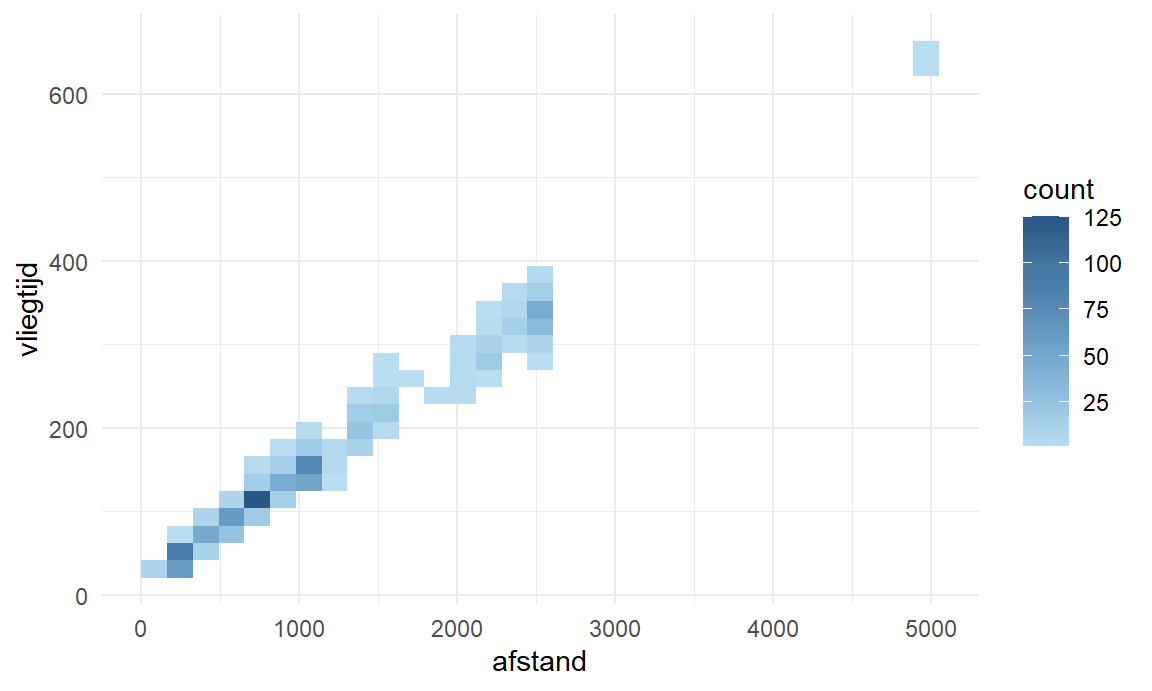
\includegraphics[width=1\linewidth]{textbook_files/figure-latex/unnamed-chunk-10-1} \caption[Scatterplot met trendlijn]{Scatterplot met trendlijn}\label{fig:unnamed-chunk-10}
\end{figure}

\begin{figure}
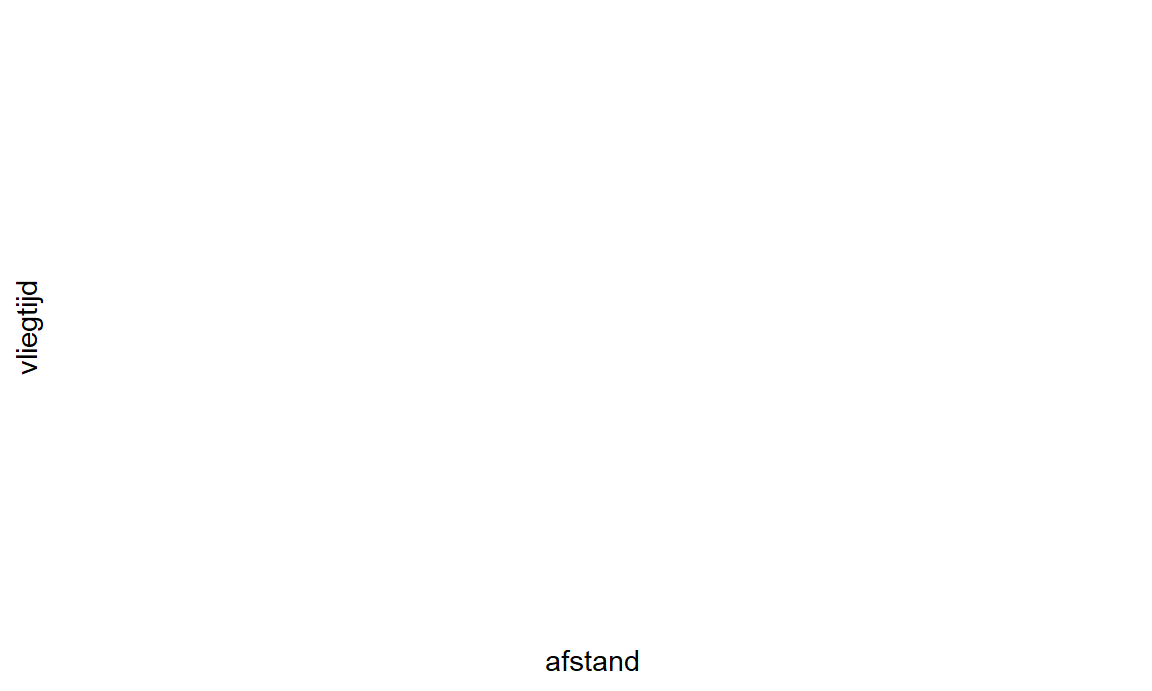
\includegraphics[width=1\linewidth]{textbook_files/figure-latex/unnamed-chunk-11-1} \caption[Hexplot met trendlijn]{Hexplot met trendlijn}\label{fig:unnamed-chunk-11}
\end{figure}

Indien de afhankelijke variabele categorisch is, dan kan je niet rechtstreeks een betekenisvolle plot maken omdat er waarschijnlijk te weinig datapunten zijn voor iedere mogelijke waarde van de onafhankelijke variabele.

\begin{itemize}
\tightlist
\item
  Wat je dan best kan doen, is de onafhankelijke continue variabele categorisch maken door deze in te delen in bins/intervallen. En dan ben je terug in de situatie waarbij de onafhankelijke variabele categorisch is. We komen hierop terug in het hoofdstuk over Data Voorbereiding.
\end{itemize}

\hypertarget{situatie-3-de-onafhankelijke-variabele-is-tijd}{%
\subsection{Situatie 3: De onafhankelijke variabele is tijd}\label{situatie-3-de-onafhankelijke-variabele-is-tijd}}

\begin{itemize}
\tightlist
\item
  Tijd kunnen we zien als continue variabele

  \begin{itemize}
  \tightlist
  \item
    Bijgevolg zelfde grafieken mogelijk als wanneer onafhankelijke variabele continue is

    \begin{itemize}
    \tightlist
    \item
      Tijd + continue afhankelijk -\textgreater{} scatterplot, 2D histograms, hex bins
    \item
      Tijd + categorisch afhankelijk -\textgreater{} probleem: tijd categoriseren (zie verder).
    \end{itemize}
  \end{itemize}
\item
  Wanneer we één enkele variabele voorstellen doorheen de tijd is er per tijdseenheid maar 1 data punt. Hieronder wordt de gemiddelde vertrekvertraging per dag getoond.\\

  \begin{figure}
  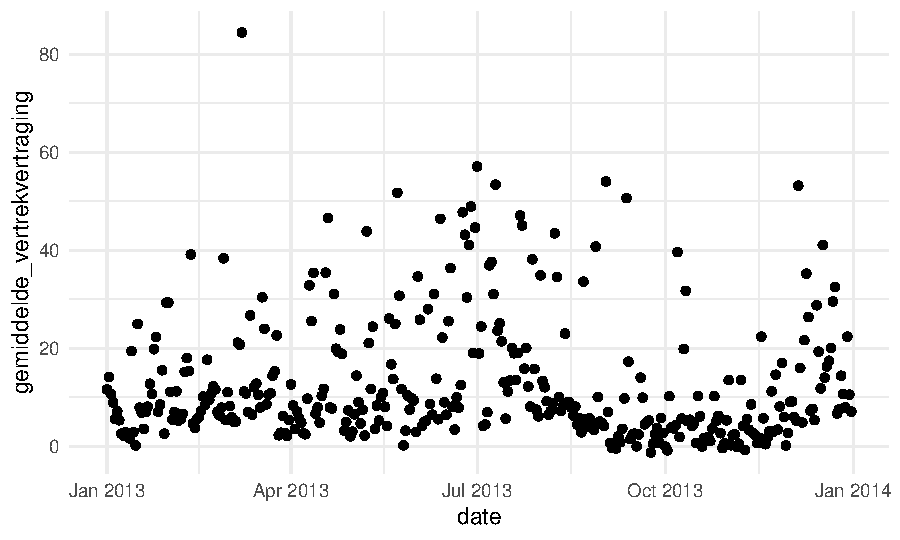
\includegraphics[width=1\linewidth]{textbook_files/figure-latex/unnamed-chunk-12-1} \caption[Puntenwolk met tijd op x-as]{Puntenwolk met tijd op x-as}\label{fig:unnamed-chunk-12}
  \end{figure}
\end{itemize}

In dat geval is het beter om in plaats van punten een lijngrafiek te gebruiken.

\begin{figure}
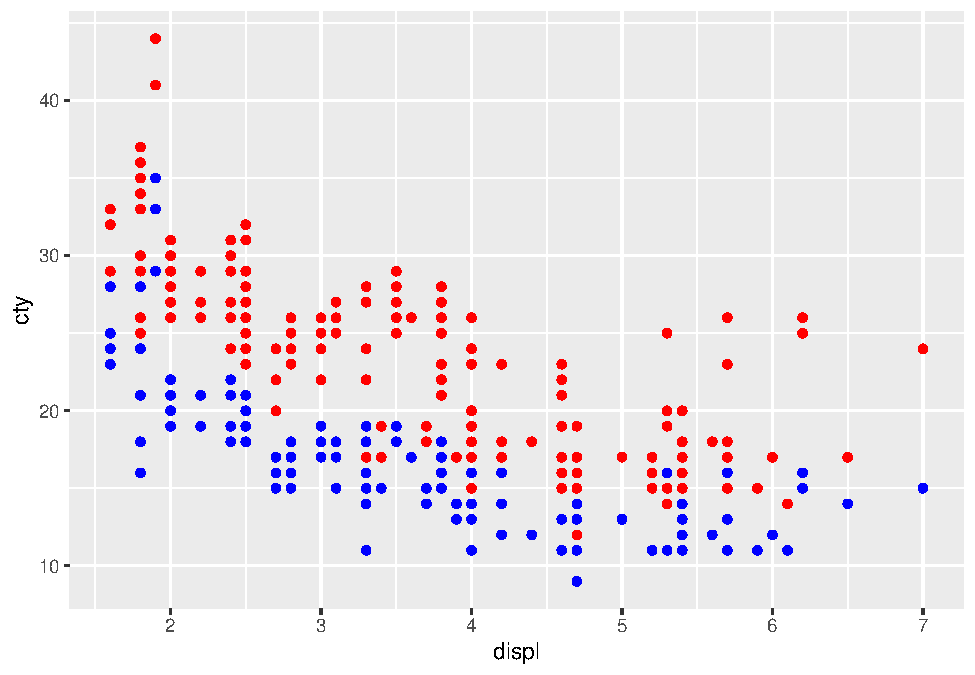
\includegraphics[width=1\linewidth]{textbook_files/figure-latex/unnamed-chunk-13-1} \caption[Lijngrafiek]{Lijngrafiek}\label{fig:unnamed-chunk-13}
\end{figure}

Indien je een beperkt aantal punten hebt (hieronder bijvoorbeeld één maand van de vluchtgegevens) kan je ervoor kiezen om zowel punten als lijnen te tonen. Op die manier is het makkelijker individuele data punten af te lezen.

\begin{figure}
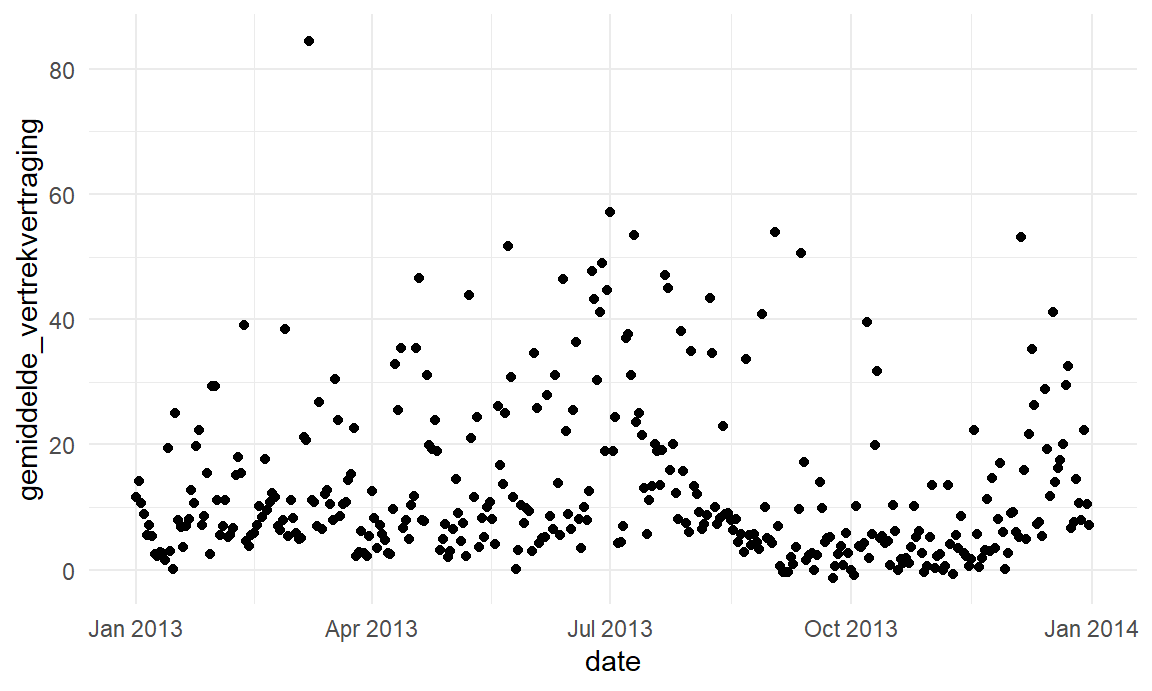
\includegraphics[width=1\linewidth]{textbook_files/figure-latex/unnamed-chunk-14-1} \caption[Lijn grafiek met punten]{Lijn grafiek met punten}\label{fig:unnamed-chunk-14}
\end{figure}

Indien we veel datapunten hebben, wat hier het geval is, kan een lijngrafiek zeer chaotisch worden. We kunnen daarom ervoor kiezen om onze tijd in te delen in categoriëen. Bijvoorbeeld, in plaats van de dagelijkse gemiddelde vertrekvertraging, kunnen we de gemiddelde vertrekvertraging per maand berekenen en tonen.

\begin{figure}
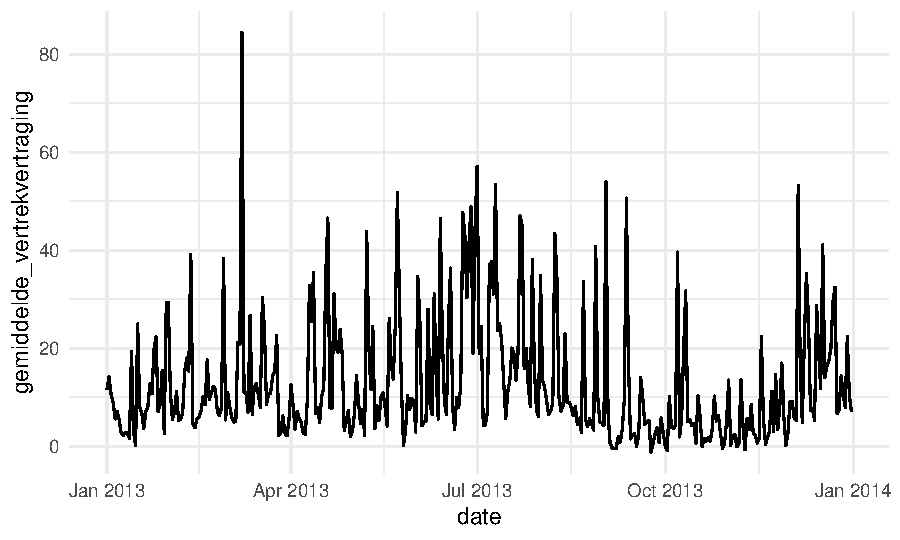
\includegraphics[width=1\linewidth]{textbook_files/figure-latex/unnamed-chunk-15-1} \caption[Lijngrafiek van gemiddelde vertrekvertraging per maand]{Lijngrafiek van gemiddelde vertrekvertraging per maand.}\label{fig:unnamed-chunk-15}
\end{figure}

\begin{itemize}
\tightlist
\item
  Op dit moment verliezen we daardoor wel veel informatie. Maar we kunnen dit nu ook beschouwen als een visualizatie van een categorische variabele (maand) t.o.v. een continue. Waardoor we de technieken voor dit type bivariate visualizaties kunnen toepassen. Bijvoorbeeld boxplots. We zien nu zowel de algemene trend als outliers. In februari was er bijvoorbeeld een dag waar de gemiddelde vertraging ver boven de normale trend lag.
\end{itemize}

\begin{figure}
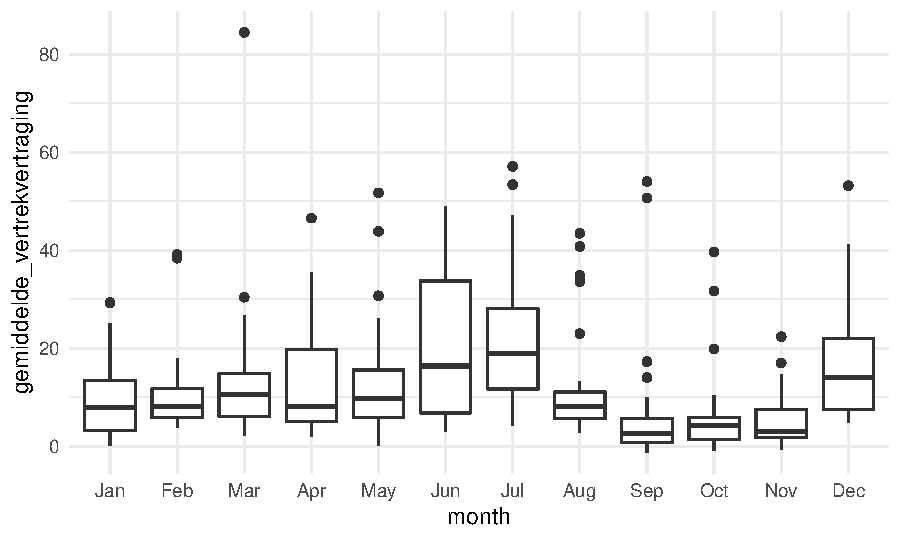
\includegraphics[width=1\linewidth]{textbook_files/figure-latex/unnamed-chunk-16-1} \caption[Boxplots van gemiddelde dagelijske vertrekvertraging voor elke maand]{Boxplots van gemiddelde dagelijske vertrekvertraging voor elke maand.}\label{fig:unnamed-chunk-16}
\end{figure}

\begin{itemize}
\tightlist
\item
  Wanneer we de tijd gecategoriseerd hebben kunnen we ook categorische variabelen weergeven als afhankelijke. Bijvoorbeeld, zijn er verschillen in het aantal vluchten per maatschappij doorheen de tijd. We kunnen hier dezelfde types grafieken als voor bivariate cat+cat visualizaties gebruiken, bijvoorbeeld stacked barcharts.
\end{itemize}

\begin{figure}
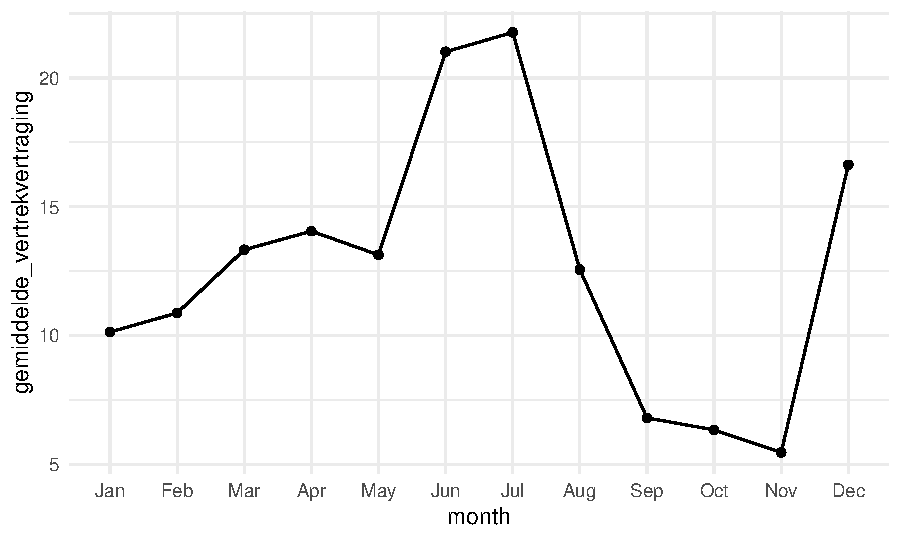
\includegraphics[width=1\linewidth]{textbook_files/figure-latex/unnamed-chunk-17-1} \caption[Verdeling van aantal vluchten over maatschappijen per maand]{Verdeling van aantal vluchten over maatschappijen per maand.}\label{fig:unnamed-chunk-17}
\end{figure}

\begin{itemize}
\tightlist
\item
  We kunnen categorizeren op maand, jaar, etc. Maar ook op tijdspecifiekere kenmerken, zoals bijvoorbeeld de dag van de week
\end{itemize}

\begin{figure}
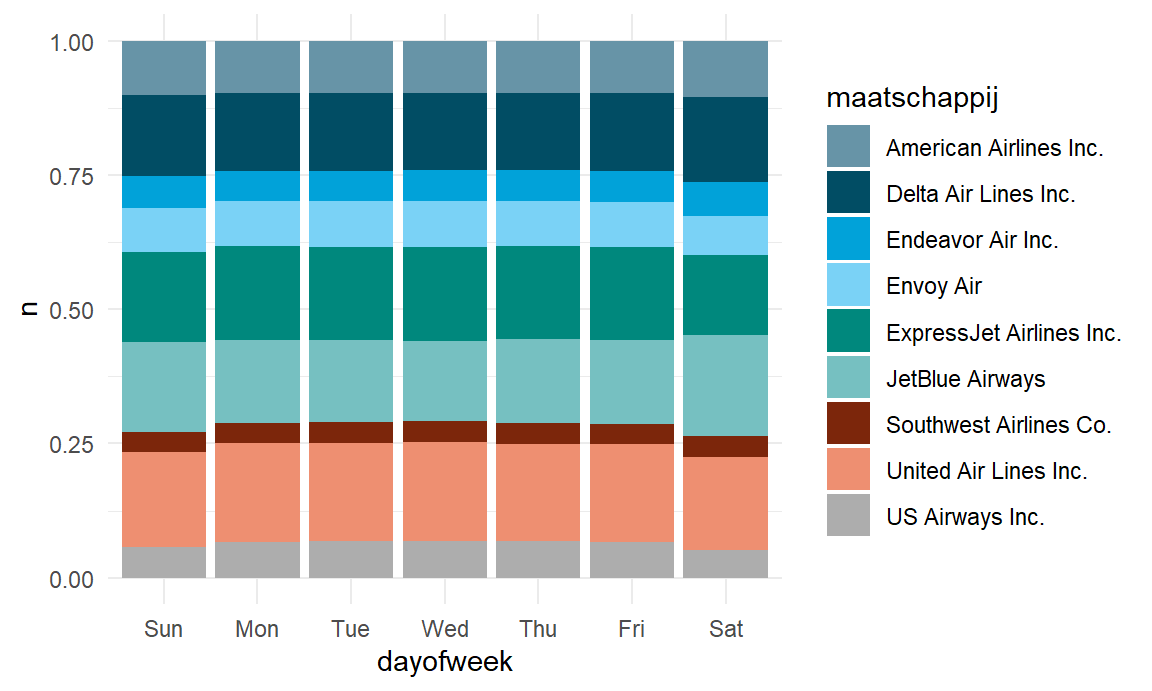
\includegraphics[width=1\linewidth]{textbook_files/figure-latex/unnamed-chunk-18-1} \caption[Verdeling van aantal vluchten over maatschappijen per dag van de week]{Verdeling van aantal vluchten over maatschappijen per dag van de week.}\label{fig:unnamed-chunk-18}
\end{figure}

\begin{itemize}
\tightlist
\item
  Of het uur van de dag
\end{itemize}

\begin{figure}
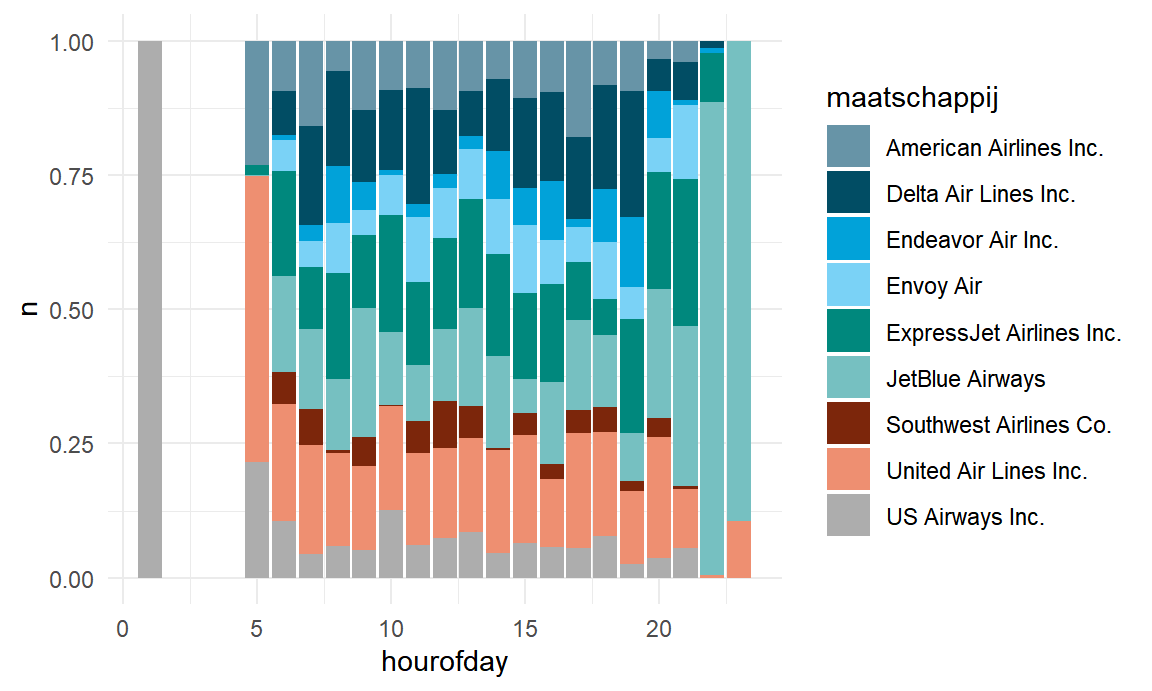
\includegraphics[width=1\linewidth]{textbook_files/figure-latex/unnamed-chunk-19-1} \caption[Verdeling van aantal vluchten over maatschappijen per vertrekuur]{Verdeling van aantal vluchten over maatschappijen per vertrekuur.}\label{fig:unnamed-chunk-19}
\end{figure}

\hypertarget{multivariate-visualisaties-meer-dan-2-variabelen}{%
\section{Multivariate visualisaties (meer dan 2 variabelen)}\label{multivariate-visualisaties-meer-dan-2-variabelen}}

\begin{itemize}
\tightlist
\item
  Datavisualisatie van patronen tussen meer dan 2 variabelen worden snel te complex om te interpreteren.
\item
  Het basisprincipe is wel eenvoudig.

  \begin{itemize}
  \tightlist
  \item
    Je hebt typisch 1 afhankelijke variabele (Y) en een aantal onafhankelijke variabelen (A, B, \ldots).
  \item
    Je visualizeert eerst Y en A (bivariaat)
  \item
    Je voegt dan de volgende variabelen (B, c, \ldots) stap voor stap toe aan de grafiek.

    \begin{itemize}
    \tightlist
    \item
      Door de bivariate grafiek te herhalen in verschillende facetten (een voor elke waarde van B).
    \item
      Door verschillende kleuren te gebruiken voor elke waarde van B
    \end{itemize}
  \end{itemize}
\item
  Bij multivariate visualisaties zijn er afhankelijk van de data types oneidig veel mogelijke grafieken die je kan maken.

  \begin{itemize}
  \tightlist
  \item
    Het is vaak afhankelijk van de data welke grafiek het ``best past''
  \item
    Enkel wanneer de onafhankelijk variabele continu is zijn de keuzes beperkt en ben je vaak genoodzaakt om deze om te zetten naar categoriëen.
  \end{itemize}
\end{itemize}

\hypertarget{voorbeeld-in-welke-mate-hangt-de-vertrek-vertraging-af-van-de-luchthaven-en-de-afstand}{%
\subsection{Voorbeeld: In welke mate hangt de vertrek vertraging af van de luchthaven en de afstand?}\label{voorbeeld-in-welke-mate-hangt-de-vertrek-vertraging-af-van-de-luchthaven-en-de-afstand}}

Stap 1. Vertraging vs.~afstand

\begin{itemize}
\tightlist
\item
  Beide continue: scatterplot
\end{itemize}

\begin{figure}
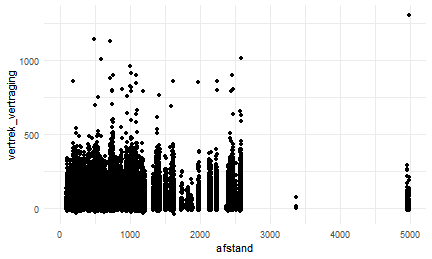
\includegraphics[width=1\linewidth]{textbook_files/figure-latex/labelke-1} \caption[Vertrekvertraging vs afstand]{Vertrekvertraging vs afstand}\label{fig:labelke}
\end{figure}

Stap 2. Voeg invloed van luchthaven toe.

\begin{itemize}
\tightlist
\item
  Optie 1: gebruik kleur om de verschillende luchthavens te differenteren. Een trendlijn kan hier helpen.
\end{itemize}

\begin{figure}
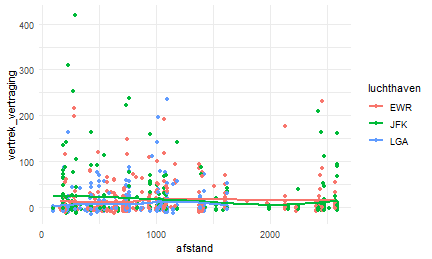
\includegraphics[width=1\linewidth]{textbook_files/figure-latex/labelke2-1} \caption[Vertrekvertraging vs afstand en luchthaven]{Vertrekvertraging vs afstand en luchthaven}\label{fig:labelke2}
\end{figure}

\begin{itemize}
\item
  Geen geweldig resultaat in dit geval.
\item
  Optie 2: Gebruik facetten voor de verschillende luchthavens.
\end{itemize}

\begin{figure*}
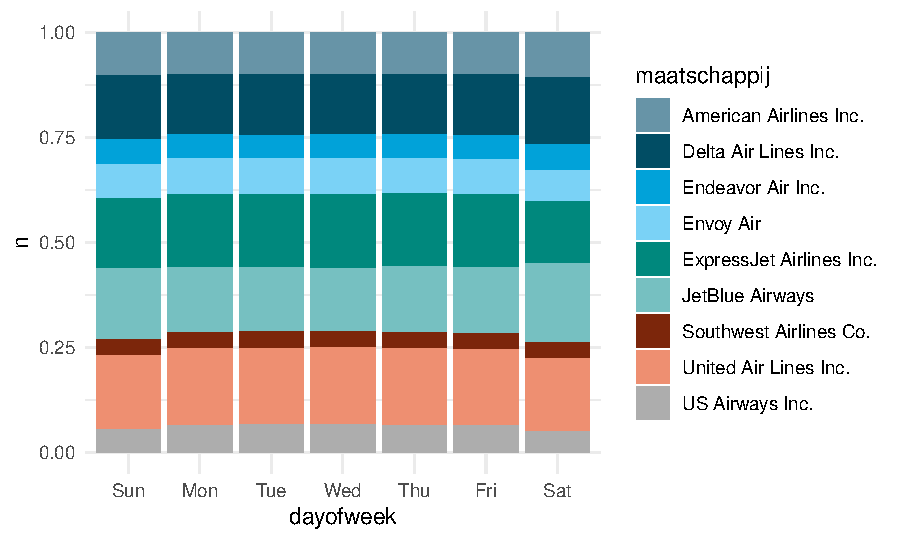
\includegraphics[width=1\linewidth]{textbook_files/figure-latex/unnamed-chunk-20-1} \caption[Vertrekvertraging vs afstand en luchthaven]{Vertrekvertraging vs afstand en luchthaven}\label{fig:unnamed-chunk-20}
\end{figure*}

\begin{itemize}
\tightlist
\item
  Optie 3: Facets, maar gebruik hex bins
\end{itemize}

\begin{figure*}
\includegraphics[width=1\linewidth]{textbook_files/figure-latex/unnamed-chunk-21-1} \caption[Vertrekvertraging vs afstand en luchthaven, hexbins]{Vertrekvertraging vs afstand en luchthaven, hexbins}\label{fig:unnamed-chunk-21}
\end{figure*}

\hypertarget{voorbeeld-multivariaat-tijd}{%
\subsection{Voorbeeld: multivariaat tijd}\label{voorbeeld-multivariaat-tijd}}

\hypertarget{situatie-1-variabelen-hebben-dezelfde-eenheid.}{%
\subsubsection{Situatie 1: Variabelen hebben dezelfde eenheid.}\label{situatie-1-variabelen-hebben-dezelfde-eenheid.}}

Voorbeeld: vertrekvertraging en aankomstvertraging. Je kan lijngrafieken tekenen met meerdere lijnen op hetzelfde assenstelsel.

\begin{figure}
\includegraphics[width=1\linewidth]{textbook_files/figure-latex/unnamed-chunk-22-1} \caption[Evolutie van 2 variabelen over tijd in één grafiek (zelfde meeteenheid)]{Evolutie van 2 variabelen over tijd in één grafiek (zelfde meeteenheid)}\label{fig:unnamed-chunk-22}
\end{figure}

\begin{itemize}
\tightlist
\item
  Of je kan er voor kiezen elke lijn in een afzonderlijk paneel te tonen
\end{itemize}

\begin{figure}
\includegraphics[width=1\linewidth]{textbook_files/figure-latex/unnamed-chunk-23-1} \caption[Evolutie van 2 variabelen over tijd in afzondelijke panels]{Evolutie van 2 variabelen over tijd in afzondelijke panels.}\label{fig:unnamed-chunk-23}
\end{figure}

\hypertarget{situatie-2-variabelen-hebben-niet-dezelfde-eenheid}{%
\subsubsection{Situatie 2: Variabelen hebben niet dezelfde eenheid}\label{situatie-2-variabelen-hebben-niet-dezelfde-eenheid}}

Voorbeeld: de gemiddelde levensverwachting en gdp per capita doorheen de tijd. In dit geval ben je genoodzaakt 2 panelen te gebruiken.

\begin{figure}
\includegraphics[width=1\linewidth]{textbook_files/figure-latex/unnamed-chunk-24-1} \caption[Evolutie van 2 variabelen met andere eenheden in afzonderlijke panels]{Evolutie van 2 variabelen met andere eenheden in afzonderlijke panels.}\label{fig:unnamed-chunk-24}
\end{figure}

Optie 2: Maak een connected scatterplot. Toon een punt voor elke meting, waarbij x en y elk een variabele voorstellen. Verbindt dat elk punt in chronologische volgorde.

\begin{figure}
\includegraphics[width=1\linewidth]{textbook_files/figure-latex/unnamed-chunk-25-1} \caption[Evolutie van 2 variabelen (levensverwachting en inkomen per capita) aan de hand van connected scatterplot]{Evolutie van 2 variabelen (levensverwachting en inkomen per capita) aan de hand van connected scatterplot.}\label{fig:unnamed-chunk-25}
\end{figure}

Variant, per continent:

\begin{figure}
\includegraphics[width=1\linewidth]{textbook_files/figure-latex/unnamed-chunk-26-1} \caption[Evolutie van 2 variabelen aan de hand van connected scatterplot - verschillende groepen]{Evolutie van 2 variabelen aan de hand van connected scatterplot - verschillende groepen.}\label{fig:unnamed-chunk-26}
\end{figure}

\hypertarget{visualisaties-voor-communicatie}{%
\section{Visualisaties voor communicatie}\label{visualisaties-voor-communicatie}}

Wanneer uiteindelijk beslist om een visualizatie te gebruiken om te communiceren, zorg ervoor dat

\begin{itemize}
\tightlist
\item
  de grafiek leesbaar is
\item
  je kleur enkel gebruikt waar nodig.
\item
  je correcte as-labels gebruikt
\item
  je geen theme gebruikt dat te druk/overheersend is
\item
  je een gepaste titel voorziet.
\end{itemize}

\hypertarget{voorbeeld-voor-goed-voor-exploratie}{%
\subsection{Voorbeeld: voor \textasciitilde{} goed voor exploratie}\label{voorbeeld-voor-goed-voor-exploratie}}

\includegraphics[width=1\linewidth]{textbook_files/figure-latex/unnamed-chunk-27-1}

\hypertarget{voorbeeld-na-goed-voor-communicatie}{%
\subsection{Voorbeeld: na \textasciitilde{} goed voor communicatie}\label{voorbeeld-na-goed-voor-communicatie}}

\includegraphics[width=1\linewidth]{textbook_files/figure-latex/unnamed-chunk-28-1}

Merk op: ver van alle grafieken getoond in dit hoofdstuk zijn goed voor communicatie zonder aanpassingen.

\hypertarget{how-charts-lie}{%
\section{How charts lie}\label{how-charts-lie}}

\hypertarget{causaliteit-vs-correlatie}{%
\subsection{Causaliteit vs correlatie}\label{causaliteit-vs-correlatie}}

\begin{itemize}
\tightlist
\item
  Van zodra er twee (or meer) variabelen zijn, gaan we op zoek naar patronen in relaties tussen de variabelen.
\item
  Het is belangrijk en essentieel te beseffen dat mensen een automatische reflex hebben om te denken in termen van oorzaak-gevolg als we kijken naar relaties tussen twee variabelen.

  \begin{itemize}
  \tightlist
  \item
    Het is echter niet omdat er een duidelijke relatie bestaat tussen twee variabelen (correlatie), dat hier sprake is van een oorzaak-gevolg verband (causaliteit).
  \item
    Bijvoorbeeld: Indien in de zomer de verkoop van paraplu's sterk stijgt, dan zal de graanopbrengst in het najaar dalen. Dit betekent niet dat de verkoop van paraplu's een impact heeft op de graanopbrengst. Wat hier waarschijnlijk gebeurt, is dat door hevige regenval in de zomermaanden, de verkoop van paraplu's is toegenomen en de graanoogst tegenvalt.

    \begin{itemize}
    \tightlist
    \item
      Soms is het intuïtief zeer onwaarschijnlijk dat de waargenomen correlatie causaliteit impliceert. Kijk hiervoor maar eens naar de voorbeelden op \url{http://www.tylervigen.com/spurious-correlations}
    \item
      Wanneer het echter plausibel is dat de waargenomen correlatie causaliteit voorstelt, is het belangrijk dat we tegen onze natuurlijke reflex in gaan en niet in termen van oorzaak-gevolg denken.
    \item
      Het aantonen van causaliteit is nooit mogelijk met descriptieve en exploratieve data analyse!
    \end{itemize}
  \end{itemize}
\end{itemize}

\hypertarget{referenties-1}{%
\section{Referenties}\label{referenties-1}}

\begin{itemize}
\tightlist
\item
  \href{https://informationisbeautiful.net/}{Information is Beautiful}
\item
  \href{https://serialmentor.com/dataviz/}{Fundamentals of Data Vizualization}
\item
  \href{https://www.r-graph-gallery.com/}{R Graph Gallery}
\item
  \href{https://www.data-to-viz.com/}{Data to viz}
\item
  \href{https://www.tylervigen.com/spurious-correlations}{Spurrious correlations}
\item
  \href{https://edition.cnn.com/2020/01/17/politics/donald-trump-2016-map-county-by-county/index.html}{Misleading election map}
\end{itemize}

\hypertarget{tutorial-data-visualisatie}{%
\chapter{{[}Tutorial{]} Data visualisatie}\label{tutorial-data-visualisatie}}

\hypertarget{voor-je-begint}{%
\section{Voor je begint}\label{voor-je-begint}}

Voordat je met deze zelfstudie begint, moet je eerst het pakket \texttt{ggplot2} installeren, als je dat nog niet gedaan hebt. Je kunt dit doen met de volgende regel code:

\begin{Shaded}
\begin{Highlighting}[]
\FunctionTok{install.packages}\NormalTok{(}\StringTok{"ggplot2"}\NormalTok{)}
\end{Highlighting}
\end{Shaded}

In ieder geval, moet je het pakket in je sessie laden.

\begin{Shaded}
\begin{Highlighting}[]
\FunctionTok{library}\NormalTok{(ggplot2)}
\end{Highlighting}
\end{Shaded}

Je hebt ook twee datasets nodig, \texttt{movies} en \texttt{diamonds}. Beide worden als .RDS bestand bij deze tutorial geleverd.

\begin{Shaded}
\begin{Highlighting}[]
\NormalTok{movies }\OtherTok{\textless{}{-}} \FunctionTok{readRDS}\NormalTok{(}\StringTok{"movies.RDS"}\NormalTok{)}
\NormalTok{diamonds }\OtherTok{\textless{}{-}} \FunctionTok{readRDS}\NormalTok{(}\StringTok{"diamonds.RDS"}\NormalTok{)}
\end{Highlighting}
\end{Shaded}

\hypertarget{introductie}{%
\section{Introductie}\label{introductie}}

Het maken van een plot met ggplot2 begint met de \texttt{ggplot()} functie. De ggplot functie heeft twee belangrijke argumenten

\begin{itemize}
\tightlist
\item
  \textbf{data}: dit definieert de dataset die voor de plot moet worden gebruikt. Dit moet een data.frame zijn.
\item
  \textbf{mapping}: de mapping zal bepalen hoe de variabelen worden \emph{mapped} op de esthetica\footnote{Hoewel het bepaalde analyses interessanter maakt als je bekend bent met de betekenis van de verschillende variabelen, is geen specifieke kennis van auto's vereist om deze tutorial te voltooien.} van de plot, zoals verderop zal worden uitgelegd. Deze mapping moet altijd worden gemaakt met de \texttt{aes()} functie .
\end{itemize}

We willen bijvoorbeeld een scatterplot maken van de films, waarbij we de x-as gebruiken voor hun budget en de y-as voor hun waardering. We roepen ggplot dan als volgt aan:

\begin{Shaded}
\begin{Highlighting}[]
\FunctionTok{ggplot}\NormalTok{(}\AttributeTok{data =}\NormalTok{ movies, }\AttributeTok{mapping =} \FunctionTok{aes}\NormalTok{(}\AttributeTok{x =}\NormalTok{ budget, }\AttributeTok{y =}\NormalTok{ rating))}
\end{Highlighting}
\end{Shaded}

\includegraphics[width=1\linewidth]{textbook_files/figure-latex/unnamed-chunk-34-1}

Zoals je ziet, creëert deze regel code een plot met de assen zoals gedefinieerd. Er worden echter geen gegevens gevisualiseerd. De reden hiervoor is dat ggplot nog niet weet hoe we het willen visualiseren. We moeten wat genoemd wordt \emph{een geometrische layer} toevoegen. Om een scatterplot te maken, die uit \emph{punten} bestaat, voegen we \texttt{geom\_point} aan de plot toe.

\begin{Shaded}
\begin{Highlighting}[]
\FunctionTok{ggplot}\NormalTok{(}\AttributeTok{data =}\NormalTok{ movies, }\AttributeTok{mapping =} \FunctionTok{aes}\NormalTok{(}\AttributeTok{x =}\NormalTok{ budget, }\AttributeTok{y =}\NormalTok{ rating)) }\SpecialCharTok{+}
  \FunctionTok{geom\_point}\NormalTok{()}
\end{Highlighting}
\end{Shaded}

\includegraphics[width=1\linewidth]{textbook_files/figure-latex/unnamed-chunk-35-1}

Dit lijkt er al meer op. Merk op dat de geometrische laag aan de plot is toegevoegd door gebruik te maken van het \texttt{+} symbool. Op deze manier kunnen meerdere lagen aan dezelfde plot worden toegevoegd, evenals titels, labels, en configuraties van de lay-out, zoals we verderop zullen zien.

Merk op dat we de mapping van de \emph{aesthetics} ook in de geometrische laag zelf kunnen plaatsen. Dit maakt onze code voorlopig iets leesbaarder, omdat we de geometrische layer en de mapping ervan op dezelfde regel plaatsen.

\begin{Shaded}
\begin{Highlighting}[]
\FunctionTok{ggplot}\NormalTok{(}\AttributeTok{data =}\NormalTok{ movies) }\SpecialCharTok{+}
  \FunctionTok{geom\_point}\NormalTok{(}\AttributeTok{mapping =} \FunctionTok{aes}\NormalTok{(}\AttributeTok{x =}\NormalTok{ budget, }\AttributeTok{y =}\NormalTok{ rating))}
\end{Highlighting}
\end{Shaded}

\includegraphics[width=1\linewidth]{textbook_files/figure-latex/unnamed-chunk-36-1}

We hebben nu onze allereerste plot gemaakt! In de volgende secties zullen we leren hoe we verschillende geom-layers en \emph{aesthetics} kunnen gebruiken en hoe we de lay-out van onze grafieken kunnen verbeteren.

\hypertarget{verschillende-geometrics}{%
\section{Verschillende geometrics}\label{verschillende-geometrics}}

Naast \texttt{geom\_point} bestaan er nog veel meer verschillende geometrieën om gegevens in ggplot te plotten. Je kunt ze bekijken door `geom\_' in het console in te typen en door de auto-complete-lijst te navigeren. Elk van de geom-layers komt met zijn eigen specifieke set van \emph{aesthetics} die in kaart gebracht kan (en soms moet) worden. In deze tutorial zullen we ons vooral richten op de volgende geometrische lagen:

\begin{itemize}
\tightlist
\item
  geom\_point
\item
  geom\_histogram
\item
  geom\_boxplot
\item
  geom\_violin
\item
  geom\_bar
\item
  geom\_col
\end{itemize}

\hypertarget{geom_point}{%
\subsection{geom\_point}\label{geom_point}}

We hebben \texttt{geom\_point} al gebruikt om onze eerste grafiek te maken, waarbij we twee variabelen in kaart brachten op de esthetica \emph{x} en \emph{y}. Er zijn echter nog enkele andere aesthetics's die met deze laag kunnen worden ingesteld. Laten we ze eens in meer detail bekijken.

\begin{itemize}
\tightlist
\item
  \textbf{x}: dit bepaalt de positie van de punten langs de x-as
\item
  \textbf{y}: hiermee bepaal je de positie van de punten langs de y-as
\item
  \textbf{color}: hiermee bepaal je de kleur van de punten
\item
  \textbf{shape}: hiermee bepaal je het type punten dat uitgezet moet worden\footnote{\includegraphics{images/tidyverse.png} Het \emph{tidyverse} is een set van pakketten voor data science die in harmonie werken omdat ze gemeenschappelijke data representaties en API ontwerp delen. Het \texttt{tidyverse}-pakket is ontworpen om het gemakkelijk te maken om kernpakketten van de tidyverse te installeren en te laden met een enkel commando. De tidyverse bevat pakketten zoals: ggplot2, dplyr, tidyr, readr, purrr, tibble, hms, stringr, lubridate, forcats, jsonlite, readxl, broom, en anderen. Hadley Wickham kan beschouwd worden als de grondlegger van het tidyverse. De beste plaats om deze pakketten te leren kennen is door dit boek te lezen: \href{http://r4ds.had.co.nz/}{R for Data Science}, geschreven door Hadley en Garret Grolemund.}
\item
  \textbf{fill}: hiermee bepaal je hoe de punten gevuld worden (voor vormen 21-25)
\item
  \textbf{size}: hiermee bepaal je de grootte van de punten
\item
  \textbf{stroke}: hiermee bepaal je de breedte van de rand
\item
  \textbf{alpha}: hiermee bepaal je de mate van doorzichtigheid
\end{itemize}

De onderstaande grafiek bijvoorbeeld toont zwarte driehoeken, gevuld met rood, met een grootte van 2. Merk op dat de positie van de driehoeken precies dezelfde is als de positie van de punten in de vorige grafiek.

\begin{Shaded}
\begin{Highlighting}[]
\FunctionTok{ggplot}\NormalTok{(}\AttributeTok{data =}\NormalTok{ movies) }\SpecialCharTok{+}
  \FunctionTok{geom\_point}\NormalTok{(}
    \AttributeTok{mapping =} \FunctionTok{aes}\NormalTok{(}\AttributeTok{x =}\NormalTok{ budget, }\AttributeTok{y =}\NormalTok{ rating),}
    \AttributeTok{shape =} \DecValTok{24}\NormalTok{,}
    \AttributeTok{fill =} \StringTok{"red"}\NormalTok{,}
    \AttributeTok{color =} \StringTok{"black"}\NormalTok{,}
    \AttributeTok{size =} \DecValTok{2}
\NormalTok{  )}
\end{Highlighting}
\end{Shaded}

\includegraphics[width=1\linewidth]{textbook_files/figure-latex/unnamed-chunk-37-1}

Maar wacht, er is hier iets belangrijks aan de hand! Terwijl de x- en y-aesthetics binnen de aes-mapping werden gedefinieerd, werden de andere aesthetic erbuiten gedefinieerd. Waarom is dat?

In feite kunnen aesthetics op twee verschillende manieren worden ingesteld:

\begin{enumerate}
\def\labelenumi{\arabic{enumi}.}
\tightlist
\item
  Ze kunnen worden \emph{mapped} naar een variabele in de dataset.
\item
  Ze kunnen worden ingesteld op één vaste waarde.
\end{enumerate}

In ons voorbeeld worden x en y gekoppeld aan twee variabelen in de gegevens, nl. budget en rating, terwijl de andere aesthetics, vorm, fill, color en size, worden ingesteld op vaste waarden. Hoewel sommige aesthetics typisch altijd gemapt worden, zoals x- en y-posities, kunnen sommige andere zowel een vaste waarde als een gemapte variabele zijn. Bijvoorbeeld, wat gebeurt er als we de kleur van punten toewijzen aan een variabele, zeg de variabele Action.

\begin{Shaded}
\begin{Highlighting}[]
\FunctionTok{ggplot}\NormalTok{(}\AttributeTok{data =}\NormalTok{ movies) }\SpecialCharTok{+}
  \FunctionTok{geom\_point}\NormalTok{(}\AttributeTok{mapping =} \FunctionTok{aes}\NormalTok{(}
    \AttributeTok{x =}\NormalTok{ budget,}
    \AttributeTok{y =}\NormalTok{ rating,}
    \AttributeTok{color =}\NormalTok{ Action}
\NormalTok{  ))}
\end{Highlighting}
\end{Shaded}

\includegraphics[width=1\linewidth]{textbook_files/figure-latex/unnamed-chunk-38-1}

We zien dat de punten nu gekleurd zijn met betrekking tot de waarde in de variabele Action. Action films krijgen een groene kleur, terwijl andere films een rode kleur krijgen, wat we kunnen zien in de legende die verscheen.

Ook de andere vaste aesthetics kunnen worden gebruikt in een mapping. Het volgende voorbeeld gebruikt de variabele Animatie voor de shape.

\begin{Shaded}
\begin{Highlighting}[]
\FunctionTok{ggplot}\NormalTok{(}\AttributeTok{data =}\NormalTok{ movies) }\SpecialCharTok{+}
  \FunctionTok{geom\_point}\NormalTok{(}\AttributeTok{mapping =} \FunctionTok{aes}\NormalTok{(}
    \AttributeTok{x =}\NormalTok{ budget,}
    \AttributeTok{y =}\NormalTok{ rating,}
    \AttributeTok{color =}\NormalTok{ Action,}
    \AttributeTok{shape =}\NormalTok{ Animation}
\NormalTok{  ))}
\end{Highlighting}
\end{Shaded}

\includegraphics[width=1\linewidth]{textbook_files/figure-latex/unnamed-chunk-39-1}

Geweldig! We begrijpen nu volledig de geom\_point laag, en de werking van de aesthetics-mapping. Nu is het tijd om enkele andere geometrische layers te bekijken. We beginnen met histogrammen.

\hypertarget{geom_histogram}{%
\subsection{geom\_histogram}\label{geom_histogram}}

De \emph{geom\_histogram} layer kan worden gebruikt om een histogram uit te zetten. Zoals je al zou moeten weten, geeft een histogram de verdeling van \textbf{een} continue variabele weer. Bijgevolg moet er alleen een x-aesthetic worden ingesteld, en geen y-aesthetic. De volledige lijst van aesthetic's is als volgt:

\begin{itemize}
\tightlist
\item
  \textbf{x}: dit bepaalt de variabele die gebruikt moet worden
\item
  \textbf{color}: hiermee bepaal je de kleur van de randen
\item
  \textbf{fill}: hiermee bepaal je met welke kleur het histogram gevuld wordt
\item
  \textbf{size}: hiermee bepaal je de grootte van de rand
\item
  \textbf{linetype}: hiermee bepaal je het type van de rand \footnote{Let op de hoofdletter I}
\item
  \textbf{alpha}: hiermee bepaal je de mate van doorzichtigheid
\item
  \textbf{weight}: hiermee bepaal je hoe de waarnemingen gewogen moeten worden. Standaard wordt elke waarneming als één gewogen.
\end{itemize}

Gebruik makend van onze kennis over het gebruik van aesthetics van voorheen, is het nu heel eenvoudig om een histogram te maken. Laten we een histogram maken voor de beoordeling van films. We geven het een zwarte rand met een witte vulling. Klaar om te proberen?

\begin{Shaded}
\begin{Highlighting}[]
\FunctionTok{ggplot}\NormalTok{(movies) }\SpecialCharTok{+}
  \FunctionTok{geom\_histogram}\NormalTok{(}\FunctionTok{aes}\NormalTok{(rating), }\AttributeTok{color =} \StringTok{"black"}\NormalTok{, }\AttributeTok{fill =} \StringTok{"white"}\NormalTok{)}
\end{Highlighting}
\end{Shaded}

\includegraphics[width=1\linewidth]{textbook_files/figure-latex/unnamed-chunk-40-1}

Merk op dat verschillende dingen werden weggelaten in deze twee lijnen van codes. In het bijzonder de argumentnaam \emph{data} in ggplot, \emph{mapping} in geom\_histogram en \emph{x} in aes. Aangezien we weten dat dit de eerste argumenten van deze functies zijn, kunnen we ze veilig weglaten, zolang we de juiste volgorde van argumenten aanhouden. We kunnen echter \emph{color} en \emph{fill} niet weglaten, omdat dit niet het tweede en derde argument van geom\_histogram zijn. Speel in geval van twijfel op veilig en schrijf de juiste argumentnamen.

Dat is echter niet het enige dat hier opvallend is. Inderdaad, er verschijnt een waarschuwing: \texttt{stat\_bin()} using \texttt{bins\ =\ 30}. Pick better value with \texttt{binwidth}. Deze waarschuwing herinnert ons aan het feit dat een standaard waarde voor het aantal bins is gekozen door geom\_histogram, die waarschijnlijk niet geschikt is voor onze grafiek. We kunnen de binbreedte veranderen door deze als argument toe te voegen aan de aanroep geom\_histogram.

\begin{Shaded}
\begin{Highlighting}[]
\FunctionTok{ggplot}\NormalTok{(movies) }\SpecialCharTok{+}
  \FunctionTok{geom\_histogram}\NormalTok{(}\FunctionTok{aes}\NormalTok{(rating), }\AttributeTok{color =} \StringTok{"black"}\NormalTok{, }\AttributeTok{fill =} \StringTok{"white"}\NormalTok{, }\AttributeTok{binwidth =} \FloatTok{0.5}\NormalTok{)}
\end{Highlighting}
\end{Shaded}

\includegraphics[width=1\linewidth]{textbook_files/figure-latex/unnamed-chunk-41-1}

Vaak heeft de binbreedte een belangrijke invloed op hoe het verkregen histogram eruit ziet. Zorgvuldig configureren van dit argument door te experimenteren met verschillende waarden is daarom belangrijk.

In de laatste plot hebben we een vaste kleur gebruikt voor het vullen van de balken van het histogram. Maar zoals we ondertussen al weten, kunnen we die ook toewijzen aan een variabele in de gegevens. Laten we de variabele \emph{Action} nog een keer gebruiken.

\begin{Shaded}
\begin{Highlighting}[]
\FunctionTok{ggplot}\NormalTok{(movies) }\SpecialCharTok{+}
  \FunctionTok{geom\_histogram}\NormalTok{(}\FunctionTok{aes}\NormalTok{(rating, }\AttributeTok{fill =}\NormalTok{ Action), }\AttributeTok{color =} \StringTok{"black"}\NormalTok{, }\AttributeTok{binwidth =} \FloatTok{0.5}\NormalTok{)}
\end{Highlighting}
\end{Shaded}

\includegraphics[width=1\linewidth]{textbook_files/figure-latex/unnamed-chunk-42-1}

Merk op hoe we het fill-argument binnen de \texttt{aes} functie hebben geplaatst. Nu is elke staaf gevuld met twee kleuren: een deel voor actie-films, en de rest voor andere films. Hoewel het niet erg duidelijk is in deze grafiek, lijkt het erop dat het centrum van het histogram voor actiefilms iets meer naar links ligt.

Merk op hoe de notatie verandert bij de overgang naar de aes-mapping: variabelennamen worden altijd zonder aanhalingstekens gebruikt, terwijl vaste aesthetics (kleuren, vormen, linetypes) met aanhalingstekens worden gebruikt (behalve voor getallen). Het is belangrijk om dit niet door elkaar te halen! Nooit aanhalingstekens rond namen van variabelen!

Standaard zijn de histogrammen voor de verschillende \emph{fills} \emph{stacked}, d.w.z. boven elkaar geplaatst. We kunnen echter het \emph{position} argument van geom\_histogram gebruiken om de staven naast elkaar te plaatsen, of \emph{dodged}.

\begin{Shaded}
\begin{Highlighting}[]
\FunctionTok{ggplot}\NormalTok{(movies) }\SpecialCharTok{+}
  \FunctionTok{geom\_histogram}\NormalTok{(}\FunctionTok{aes}\NormalTok{(rating, }\AttributeTok{fill =}\NormalTok{ Action),}
    \AttributeTok{color =} \StringTok{"black"}\NormalTok{, }\AttributeTok{binwidth =} \FloatTok{0.5}\NormalTok{, }\AttributeTok{position =} \StringTok{"dodge"}
\NormalTok{  )}
\end{Highlighting}
\end{Shaded}

\includegraphics[width=1\linewidth]{textbook_files/figure-latex/unnamed-chunk-43-1}

Met position = ``dodge'' worden de balken voor actiefilms en niet-actiefilms naast elkaar geplaatst, in plaats van boven elkaar. We kunnen teruggaan naar de oorspronkelijke grafiek door position = ``stack'' te gebruiken, of door dit argument weg te laten. Later zullen we zien hoe we beter met dergelijke zaken kunnen omgaan door gebruik te maken van rasters van verschillende plots, of zogenaamde \emph{facets}.

Alles goed tot nu toe? Laten we eens kijken naar een andere manier om de verdeling van continue variabelen te visualiseren, namelijk de boxplot.

\hypertarget{geom_boxplot}{%
\subsection{geom\_boxplot}\label{geom_boxplot}}

Een boxplot plaatst de waarden van de variabele op de y-as. Dus, als we een boxplot willen maken voor ratings, moeten we \texttt{aes(y\ =\ ratings)} gebruiken. Er is hier echter iets tricky aan de hand\ldots{} De aesthetics voor geom\_boxplot is de volgende

\begin{itemize}
\tightlist
\item
  \textbf{x}: dit definieert de variabele die voor de x-as wordt gebruikt
\item
  \textbf{y}: dit definieert de variabele voor de y-as
\item
  \textbf{color}: hiermee bepaal je de kleur van de randen
\item
  \textbf{fill}: hiermee bepaal je hoe de boxplot wordt opgevuld
\item
  \textbf{size}: hiermee bepaal je de grootte van de rand
\item
  \textbf{linetype}: hiermee bepaal je het type van de rand
\item
  \textbf{alpha}: Hiermee bepaal je de mate van doorzichtigheid
\end{itemize}

Dus, de boxplot heeft zowel een x-variabele als een y-variabele nodig? Dat lijkt op het eerste gezicht vreemd. De reden hierachter is dat in de filosofie van ggplot, altijd \emph{iets} moet geplot worden op zowel de x- als de y-as. Hoewel alleen een x-variabele wordt gegeven aan een histogram, zal het frequenties berekenen om op de y-as te plotten. Bij boxplots gebeurt dat echter niet. Bijgevolg moet de x-as worden gebruikt om verschillende categorieën in kaart te brengen waarvan de verdeling vervolgens kan worden vergeleken. Zo kunnen we bijvoorbeeld de waardering voor actiefilms vergelijken met die voor andere films.

\begin{Shaded}
\begin{Highlighting}[]
\FunctionTok{ggplot}\NormalTok{(movies) }\SpecialCharTok{+}
  \FunctionTok{geom\_boxplot}\NormalTok{(}\FunctionTok{aes}\NormalTok{(Action, rating))}
\end{Highlighting}
\end{Shaded}

\includegraphics[width=1\linewidth]{textbook_files/figure-latex/unnamed-chunk-44-1}

Hier zien we dat, zoals we al vermoedden, actiefilms een lagere waardering hebben in vergelijking met andere films. We kunnen verder de kleur en de vulling van de boxplot veranderen zoals voorheen, alsook het linetype, de grootte van de rand, of de transparantie.

Maar wat als we gewoon een boxplot willen tekenen van de totale waardering, zonder een variabele te moeten specificeren voor de x-as? Een kleine workaround is hier nodig. Een mogelijkheid is om een \emph{empty string} te gebruiken voor de x-as toewijzing.

\begin{Shaded}
\begin{Highlighting}[]
\FunctionTok{ggplot}\NormalTok{(movies) }\SpecialCharTok{+}
  \FunctionTok{geom\_boxplot}\NormalTok{(}\FunctionTok{aes}\NormalTok{(}\StringTok{""}\NormalTok{, rating))}
\end{Highlighting}
\end{Shaded}

\includegraphics[width=1\linewidth]{textbook_files/figure-latex/unnamed-chunk-45-1}

Merk op dat dit het label ``x'' creëert voor de x-as, waar we normaal de naam van de variabele zouden vinden die erop is weergegeven. Later zullen we zien hoe we dit label kunnen weglaten om onze grafiek een beetje mooier te maken.

\hypertarget{geom_violin}{%
\subsection{geom\_violin}\label{geom_violin}}

De violin-plot is vergelijkbaar met de boxplot, maar geeft in meer detail weer waar de massa van de waarden zich bevindt. De aesthetics is dezelfde als bij een boxplot.

\begin{itemize}
\tightlist
\item
  \textbf{x}: dit definieert de variabele die voor de x-as wordt gebruikt
\item
  \textbf{y}: dit definieert de variabele voor de y-as
\item
  \textbf{color}: hiermee bepaal je de kleur van de randen
\item
  \textbf{fill}: hiermee bepaal je hoe de plot wordt opgevuld
\item
  \textbf{size}: hiermee bepaal je de grootte van de rand
\item
  \textbf{linetype}: hiermee bepaal je het type van de rand
\item
  \textbf{alpha}: Hiermee bepaal je de mate van doorzichtigheid
\end{itemize}

Laten we dezelfde grafieken maken, nu met de violin-plot.

\begin{Shaded}
\begin{Highlighting}[]
\FunctionTok{ggplot}\NormalTok{(movies) }\SpecialCharTok{+}
  \FunctionTok{geom\_violin}\NormalTok{(}\FunctionTok{aes}\NormalTok{(Action, rating))}
\end{Highlighting}
\end{Shaded}

\includegraphics[width=1\linewidth]{textbook_files/figure-latex/unnamed-chunk-46-1}

Het is nu waarschijnlijk wel duidelijk waar dit type grafiek zijn naam aan te danken heeft. Zoals je kunt zien, houden violin-plots het midden tussen boxplots en histogrammen. Omdat hun breedte genormaliseerd is, kunnen ze beter gebruikt worden voor vergelijkingen. Ook hier kunnen we dezelfde workaround gebruiken als we de algemene verdeling willen plotten.

\begin{Shaded}
\begin{Highlighting}[]
\FunctionTok{ggplot}\NormalTok{(movies) }\SpecialCharTok{+}
  \FunctionTok{geom\_violin}\NormalTok{(}\FunctionTok{aes}\NormalTok{(}\StringTok{""}\NormalTok{, rating))}
\end{Highlighting}
\end{Shaded}

\includegraphics[width=1\linewidth]{textbook_files/figure-latex/unnamed-chunk-47-1}

Tot nu toe hebben we drie verschillende manieren gezien om de verdeling van continue variabelen te analyseren. Nu gaan we kijken naar barplots, die kunnen worden gebruikt om categorische verdelingen weer te geven.

\hypertarget{geom_bar}{%
\subsection{geom\_bar}\label{geom_bar}}

Net als een histogram, heeft een barplot alleen een x variabele nodig. Het verschil is dat deze variabele categorisch moet zijn, terwijl ze voor histogrammen continu moet zijn. De volledige lijst van aesthetics is de volgende:

\begin{itemize}
\tightlist
\item
  \textbf{x}: dit bepaalt de variabele die voor de x-as gebruikt wordt
\item
  \textbf{color}: hiermee bepaal je de kleur van de randen
\item
  \textbf{fill}: hiermee bepaal je hoe de balken gevuld worden
\item
  \textbf{size}: hiermee bepaal je de grootte van de rand
\item
  \textbf{linetype}: hiermee bepaal je het type van de rand
\item
  \textbf{alpha}: hiermee bepaal je de mate van transparantie
\item
  \textbf{weight}: hiermee bepaal je hoe de waarnemingen gewogen moeten worden. Standaard wordt elke waarneming als één gewogen.
\end{itemize}

We kunnen een eenvoudig staafdiagram maken dat laat zien hoeveel actiefilms er zijn, en hoeveel andere films, en wel als volgt.

\begin{Shaded}
\begin{Highlighting}[]
\FunctionTok{ggplot}\NormalTok{(movies) }\SpecialCharTok{+}
  \FunctionTok{geom\_bar}\NormalTok{(}\FunctionTok{aes}\NormalTok{(Action))}
\end{Highlighting}
\end{Shaded}

\includegraphics[width=1\linewidth]{textbook_files/figure-latex/unnamed-chunk-48-1}

Verder kunnen we hier nog kleuren aan toevoegen, volgens het aantal Animatiefilms. We zien onmiddellijk dat er bijna geen actiefilms zijn die ook animatiefilms zijn.

\begin{Shaded}
\begin{Highlighting}[]
\FunctionTok{ggplot}\NormalTok{(movies) }\SpecialCharTok{+}
  \FunctionTok{geom\_bar}\NormalTok{(}\FunctionTok{aes}\NormalTok{(Action, }\AttributeTok{fill =}\NormalTok{ Animation))}
\end{Highlighting}
\end{Shaded}

\includegraphics[width=1\linewidth]{textbook_files/figure-latex/unnamed-chunk-49-1}

We kunnen hetzelfde doen voor Romantische en Komedie films.

\begin{Shaded}
\begin{Highlighting}[]
\FunctionTok{ggplot}\NormalTok{(movies) }\SpecialCharTok{+}
  \FunctionTok{geom\_bar}\NormalTok{(}\FunctionTok{aes}\NormalTok{(Romance, }\AttributeTok{fill =}\NormalTok{ Comedy))}
\end{Highlighting}
\end{Shaded}

\includegraphics[width=1\linewidth]{textbook_files/figure-latex/unnamed-chunk-50-1}

Daarentegen is hier te zien dat ongeveer de helft van de romantische films ook komedies zijn, wat meer is in vergelijking met niet-romantische films.

Vergeet niet dat we in het geval van histogrammen de position konden veranderen in ``dodge'', waardoor de balken naast elkaar kwamen te staan. Hetzelfde kan hier worden gedaan.

\begin{Shaded}
\begin{Highlighting}[]
\FunctionTok{ggplot}\NormalTok{(movies) }\SpecialCharTok{+}
  \FunctionTok{geom\_bar}\NormalTok{(}\FunctionTok{aes}\NormalTok{(Romance, }\AttributeTok{fill =}\NormalTok{ Comedy), }\AttributeTok{position =} \StringTok{"dodge"}\NormalTok{)}
\end{Highlighting}
\end{Shaded}

\includegraphics[width=1\linewidth]{textbook_files/figure-latex/unnamed-chunk-51-1}

Een derde mogelijkheid die voor de position beschikbaar is, is de staven te verlengen zodat zij dezelfde hoogte hebben. Het resultaat is dat we de verdeling van de waarden als een deel van een geheel zullen waarnemen. In plaats van de absolute frequentie zullen de labels op de y-as nu de procentpunten weergeven.

\begin{Shaded}
\begin{Highlighting}[]
\FunctionTok{ggplot}\NormalTok{(movies) }\SpecialCharTok{+}
  \FunctionTok{geom\_bar}\NormalTok{(}\FunctionTok{aes}\NormalTok{(Romance, }\AttributeTok{fill =}\NormalTok{ Comedy), }\AttributeTok{position =} \StringTok{"fill"}\NormalTok{)}
\end{Highlighting}
\end{Shaded}

\includegraphics[width=1\linewidth]{textbook_files/figure-latex/unnamed-chunk-52-1}

Tenslotte, als we dit willen doen om de verdeling van één variabele te tonen, kunnen we dezelfde workaround gebruiken als voorheen en de x-aesthetic op ``\,'' zetten. De plot hieronder zal het deel van alle films tonen die komedies zijn.\footnote{Merk op dat het in dergelijke gevallen volkomen logisch is de plot minder breed te maken, of hem 90 graden om te draaien en minder hoog te maken. We komen hier later op terug.}

\begin{Shaded}
\begin{Highlighting}[]
\FunctionTok{ggplot}\NormalTok{(movies) }\SpecialCharTok{+}
  \FunctionTok{geom\_bar}\NormalTok{(}\FunctionTok{aes}\NormalTok{(}\StringTok{""}\NormalTok{, }\AttributeTok{fill =}\NormalTok{ Comedy), }\AttributeTok{position =} \StringTok{"fill"}\NormalTok{)}
\end{Highlighting}
\end{Shaded}

\includegraphics[width=1\linewidth]{textbook_files/figure-latex/unnamed-chunk-53-1}

\hypertarget{geom_col}{%
\subsection{geom\_col}\label{geom_col}}

Wanneer we geom\_bar gebruiken, wordt de hoogte van de balken berekend aan de hand van de frequentie van de categorische variabele. Soms willen we echter een staafdiagram plotten met waarden die al in de data zitten, of waarden die we zelf hebben berekend. Bijvoorbeeld, wat als we een staafdiagram willen met het budget van een reeks films? In zo'n geval kunnen we \emph{geom\_col} gebruiken. ``col'' geeft aan dat we een kolom in de gegevens willen gebruiken om de hoogte van de balken in te stellen. De aesthetics is hetzelfde voor geom\_bar, alleen moeten we nu een variabele specificeren voor de y-as uiteraard.

\begin{itemize}
\tightlist
\item
  \textbf{x}: dit bepaalt de variabele die voor de x-as gebruikt wordt
\item
  \textbf{x}: dit bepaalt de variabele die voor de y-as gebruikt wordt
\item
  \textbf{color}: hiermee bepaal je de kleur van de randen
\item
  \textbf{fill}: hiermee bepaal je hoe de balken gevuld worden
\item
  \textbf{size}: hiermee bepaal je de grootte van de rand
\item
  \textbf{linetype}: hiermee bepaal je het type van de rand
\item
  \textbf{alpha}: hiermee bepaal je de mate van transparantie
\item
  \textbf{weight}: hiermee bepaal je hoe de waarnemingen gewogen moeten worden. Standaard wordt elke waarneming als één gewogen.
\end{itemize}

Laten we een staafdiagram maken van het budget van alle films uit 2004 waarvan het budget hoger was dan 100 miljoen.

\begin{Shaded}
\begin{Highlighting}[]
\FunctionTok{filter}\NormalTok{(movies, year }\SpecialCharTok{==} \DecValTok{2004}\NormalTok{, budget }\SpecialCharTok{\textgreater{}} \DecValTok{100000000}\NormalTok{) }\SpecialCharTok{\%\textgreater{}\%}
  \FunctionTok{ggplot}\NormalTok{() }\SpecialCharTok{+}
  \FunctionTok{geom\_col}\NormalTok{(}\FunctionTok{aes}\NormalTok{(title, budget))}
\end{Highlighting}
\end{Shaded}

\includegraphics[width=1\linewidth]{textbook_files/figure-latex/unnamed-chunk-54-1}

Zie je iets vreemds in de code? Maak je geen zorgen als je de eerste regel niet begrijpt. Al wat je moet weten is dat we films uit 2004 hebben gefilterd met een budget hoger dan 100 miljoen. Het vreemd uitziende \%\textgreater\% symbool zal ervoor zorgen dat deze gegevens doorgegeven worden aan ggplot. We zullen hier in een andere sessie op terugkomen. \footnote{\includegraphics{images/pipe.jpg} Het piping-symbool werd voor het eerst geïntroduceerd in het pakket \texttt{magrittr}, genoemd naar de Belgische surrealistische kunstenaar René Magritte, bekend van zijn schilderij \emph{The Threachery of Images}, oftewel \emph{Ceci n'est pas un pipe}.}

We hebben nu filmtitels uitgezet op de x-as en budget op de y-as. Geweldig! Of toch niet? De waarden op de x-as zijn wat onoverzichtelijk en onleesbaar. Het is nu tijd om aandacht te besteden aan de layout van onze plots!

\hypertarget{other-geometrics}{%
\subsection{Other geometrics}\label{other-geometrics}}

Tot dusver hebben we de belangrijkste geom-layers gebruikt om eenvoudige visualisaties te maken: scatterplots, histogrammen, boxplots, violinplots en barplots. We hebben echter slechts het topje van de ijsberg besproken, want er bestaan nog veel meer types, sommige eenvoudig en sommige meer geavanceerd. Een overzicht van alle geoms en hun toepassingen kan gevonden worden in de \href{https://www.rstudio.com/wp-content/uploads/2015/12/ggplot2-cheatsheet-2.0.pdf}{ggplot Cheat Sheet}, waarvan hier een uittreksel wordt getoond. Wees niet bang om iets uit te proberen!

\includegraphics{images/geoms.PNG}

\hypertarget{layout-van-onze-grafieken-verbeteren}{%
\section{Layout van onze grafieken verbeteren}\label{layout-van-onze-grafieken-verbeteren}}

Tot nu toe hebben we vooral gekeken naar verschillende soorten plots en hoe we die op onze gegevens kunnen plotten. In deze sectie zullen we ons concentreren op de presentatie van de plot, bv. titels, kleuren, assen, enz. De in dit deel geïntroduceerde concepten kunnen voor elk type plot worden toegepast, ongeacht welk geometrisch object wordt gebruikt.

In dit deel zal de dataset ``diamanten'' worden gebruikt. De onderstaande plot zal als uitgangspunt worden gebruikt. \footnote{De table van een diamant verwijst naar het vlakke facet van de diamant dat kan worden gezien wanneer de steen naar boven wordt gekeerd. De diepte van een diamant is de hoogte (in millimeters) gemeten van de culet tot de tafel.}

\begin{Shaded}
\begin{Highlighting}[]
\FunctionTok{ggplot}\NormalTok{(diamonds) }\SpecialCharTok{+}
  \FunctionTok{geom\_point}\NormalTok{(}\FunctionTok{aes}\NormalTok{(table, depth, }\AttributeTok{color =}\NormalTok{ cut))}
\end{Highlighting}
\end{Shaded}

\includegraphics[width=1\linewidth]{textbook_files/figure-latex/unnamed-chunk-55-1}

\hypertarget{titels}{%
\subsection{Titels}\label{titels}}

Een van de belangrijkste dingen om aan onze plot toe te voegen zijn titels. Titels worden gebruikt om betekenis te geven aan zowel de assen als de plot zelf. De meest eenvoudige manier om titels toe te voegen is door gebruik te maken van de functie \texttt{labs()}. In deze functie kunnen o.a. volgende argumenten worden ingesteld: de titel, de ondertitel, x voor het x label en y voor het y label. De labs functie kan gewoon aan de plot worden toegevoegd als een extra laag.

\begin{Shaded}
\begin{Highlighting}[]
\FunctionTok{data}\NormalTok{(}\StringTok{"diamonds"}\NormalTok{)}
\FunctionTok{ggplot}\NormalTok{(diamonds) }\SpecialCharTok{+}
  \FunctionTok{geom\_point}\NormalTok{(}\FunctionTok{aes}\NormalTok{(table, depth, }\AttributeTok{color =}\NormalTok{ cut)) }\SpecialCharTok{+}
  \FunctionTok{labs}\NormalTok{(}
    \AttributeTok{title =} \StringTok{"Comparing table and depth of diamonds"}\NormalTok{,}
    \AttributeTok{subtitle =} \StringTok{"What combination of table and depth gives good quality diamonds?"}\NormalTok{,}
    \AttributeTok{x =} \StringTok{"Table"}\NormalTok{,}
    \AttributeTok{y =} \StringTok{"Depth"}
\NormalTok{  )}
\end{Highlighting}
\end{Shaded}

\includegraphics[width=1\linewidth]{textbook_files/figure-latex/unnamed-chunk-56-1}

Je zult zien dat onze grafiek er al veel beter uitziet als er titels aan toegevoegd zijn! Er is echter nog veel meer te verbeteren.

\hypertarget{theme}{%
\subsection{Theme}\label{theme}}

Het \emph{theme} van een plot bepaalt het algemene uiterlijk: de rasterlijnen, de achtergrond, de grootte van de tekst, titels en legende, de positie van de legende, enz. Het thema kan handmatig worden gedefinieerd door een \texttt{theme()} laag toe te voegen aan de plot en door de benodigde argumenten in te stellen. (Je kunt kijken op ?theme om te zien welke argumenten beschikbaar zijn). Dit is echter een omslachtige aanpak. Gelukkig zijn er enkele voorgedefinieerde thema's voorzien in ggplot:

\begin{itemize}
\tightlist
\item
  \textbf{theme\_gray}: het standaardthema (tot nu toe gebruikt)
\item
  \textbf{theme\_bw}: een thema voor zwart-wit plots
\item
  \textbf{theme\_dark}: een donker thema voor contrast
\item
  \textbf{theme\_classic}: een minimaal thema
\item
  \textbf{theme\_light}: een ander minimaal thema
\item
  \textbf{theme\_linedraw}: nog een minimaal thema
\item
  \textbf{theme\_minimal}: nog een minimaal thema
\item
  \textbf{theme\_void}: een leeg thema
\end{itemize}

Voel je vrij om met sommige van deze thema's te experimenteren. Bij voorkeur kunt u een aantal van de minimale thema's gebruiken. Hier, gebruikten we het thema\_light thema. \footnote{Voor de meeste lagen is het niet belangrijk in welke volgorde ze aan een plot worden toegevoegd. Echter, als je handmatig wijzigingen aanbrengt met \texttt{theme}, zorg er dan voor dat je ze na een voorgedefinieerd thema plaatst, anders zullen je wijzigingen worden overschreven.}

\begin{Shaded}
\begin{Highlighting}[]
\FunctionTok{ggplot}\NormalTok{(diamonds) }\SpecialCharTok{+}
  \FunctionTok{geom\_point}\NormalTok{(}\FunctionTok{aes}\NormalTok{(table, depth, }\AttributeTok{color =}\NormalTok{ cut)) }\SpecialCharTok{+}
  \FunctionTok{labs}\NormalTok{(}
    \AttributeTok{title =} \StringTok{"Comparing table and depth of diamonds"}\NormalTok{,}
    \AttributeTok{subtitle =} \StringTok{"What combination of table and depth gives good quality diamonds?"}\NormalTok{,}
    \AttributeTok{x =} \StringTok{"Table"}\NormalTok{,}
    \AttributeTok{y =} \StringTok{"Depth"}
\NormalTok{  ) }\SpecialCharTok{+}
  \FunctionTok{theme\_light}\NormalTok{()}
\end{Highlighting}
\end{Shaded}

\includegraphics[width=1\linewidth]{textbook_files/figure-latex/unnamed-chunk-57-1}

Wanneer je nog niet tevreden bent met één van deze thema's, kunt je het pakket \texttt{ggthemes} installeren om nog meer thema's te verkrijgen, zoals het thema van \emph{The Economist}, \emph{fivethirtyeight.com}, of \emph{Google Docs}.

\hypertarget{het-couxf6rdinatenstelsel}{%
\subsection{Het coördinatenstelsel}\label{het-couxf6rdinatenstelsel}}

Het uiterlijk van de grafiek wordt niet alleen bepaald door de titels en de grafieken. Ook de assen in het assenstelsel verdienen de nodige aandacht. Een van de dingen die moeten worden bepaald zijn de grenzen van het coördinatenstelsel. Dit kan worden gedaan met de functie \texttt{coord\_cartesian} en zijn argumenten \emph{xlim} en \emph{ylim}. Beide argumenten verwachten een numerieke vector van lengte twee. Laten we eens kijken hoe dit werkt in ons voorbeeld. \footnote{Een cartesisch coördinatenstelsel is een coördinatenstelsel dat elk punt op unieke wijze in een vlak specificeert door een paar numerieke coördinaten, die de getekende afstanden tot het punt zijn van twee vaste loodrecht op elkaar staande gerichte lijnen, gemeten in dezelfde lengte-eenheid. Het is vernoemd naar wetenschapper René Descartes.}

\begin{Shaded}
\begin{Highlighting}[]
\FunctionTok{ggplot}\NormalTok{(diamonds) }\SpecialCharTok{+}
  \FunctionTok{geom\_point}\NormalTok{(}\FunctionTok{aes}\NormalTok{(table, depth, }\AttributeTok{color =}\NormalTok{ cut)) }\SpecialCharTok{+}
  \FunctionTok{labs}\NormalTok{(}
    \AttributeTok{title =} \StringTok{"Comparing table and depth of diamonds"}\NormalTok{,}
    \AttributeTok{subtitle =} \StringTok{"What combination of table and depth gives good quality diamonds?"}\NormalTok{,}
    \AttributeTok{x =} \StringTok{"Table"}\NormalTok{,}
    \AttributeTok{y =} \StringTok{"Depth"}
\NormalTok{  ) }\SpecialCharTok{+}
  \FunctionTok{theme\_light}\NormalTok{() }\SpecialCharTok{+}
  \FunctionTok{coord\_cartesian}\NormalTok{(}\AttributeTok{xlim =} \FunctionTok{c}\NormalTok{(}\DecValTok{45}\NormalTok{, }\DecValTok{75}\NormalTok{), }\AttributeTok{ylim =} \FunctionTok{c}\NormalTok{(}\DecValTok{50}\NormalTok{, }\DecValTok{75}\NormalTok{))}
\end{Highlighting}
\end{Shaded}

\includegraphics[width=1\linewidth]{textbook_files/figure-latex/unnamed-chunk-58-1}

We hebben nu de x-as beperkt tot het interval van 45 tot 75, terwijl we de y-as hebben beperkt tot het interval 50 tot 75. Er zijn enkele alternatieven voor het cartesisch coördinatenstelsel die minder vaak worden gebruikt:

\begin{itemize}
\tightlist
\item
  coord\_equal: een coördinatenstelsel waarbij de x-as en de y-as gelijk geschaald zijn (d.w.z. verhouding = 1)
\item
  coord\_fixed: een assenstelsel met een vaste verhouding (maar niet noodzakelijk 1)
\item
  coord\_polar: een coördinatensysteem voor polaire plots, of cirkeldiagrammen
\item
  coord\_map: een assenstelsel voor het plotten van geografische data.
\end{itemize}

Naast het instellen van de grenzen van het coordinatensysteem, kunnen we ook de breaks op de x-as en de y-as instellen. Dit kan respectievelijk met de functies \texttt{scale\_x\_continuous} en \texttt{scale\_y\_continuous}. Beide functies hebben een \emph{breaks} argument. Dit argument kan worden gegeven als een vector van waarden die als labels op de as moeten worden geplot.\footnote{Merk op dat de scale\_.\_continuous functies ook een argument \texttt{limits} hebben om de grenzen van de assen in te stellen, dat gebruikt kan worden in plaats van coord\_cartesion. Er is echter een belangrijk verschil. Coord\_cartesian zal inzoomen op de grenzen zonder andere datapunten weg te gooien. Het instellen van de grenzen binnen de scale-functies echter, zal datapunten weggooien en kan je visualisatie vertekenen. \includegraphics{images/zoom.png}} We kunnen de functie \texttt{seq} gebruiken om deze vector te maken: d.w.z. \texttt{seq(0,10,5)} zal een vector teruggeven die begint bij 0 en oploopt tot tien met intervallen van 5. \footnote{De titels van de assen die we gedefinieerd hebben met de \texttt{labs} functie kunnen ook ingesteld worden in de scale-functies met het argument \texttt{name}. Naarmate je meer vertrouwd raakt met het gebruik van ggplot2, zul je vaak merken dat er meerdere manieren zijn om hetzelfde doel te bereiken.}

\begin{Shaded}
\begin{Highlighting}[]
\FunctionTok{ggplot}\NormalTok{(diamonds) }\SpecialCharTok{+}
  \FunctionTok{geom\_point}\NormalTok{(}\FunctionTok{aes}\NormalTok{(table, depth, }\AttributeTok{color =}\NormalTok{ cut)) }\SpecialCharTok{+}
  \FunctionTok{labs}\NormalTok{(}
    \AttributeTok{title =} \StringTok{"Comparing table and depth of diamonds"}\NormalTok{,}
    \AttributeTok{subtitle =} \StringTok{"What combination of table}
\StringTok{         and depth gives good quality diamonds?"}\NormalTok{,}
    \AttributeTok{x =} \StringTok{"Table"}\NormalTok{,}
    \AttributeTok{y =} \StringTok{"Depth"}
\NormalTok{  ) }\SpecialCharTok{+}
  \FunctionTok{theme\_light}\NormalTok{() }\SpecialCharTok{+}
  \FunctionTok{coord\_cartesian}\NormalTok{(}\AttributeTok{xlim =} \FunctionTok{c}\NormalTok{(}\DecValTok{45}\NormalTok{, }\DecValTok{75}\NormalTok{), }\AttributeTok{ylim =} \FunctionTok{c}\NormalTok{(}\DecValTok{50}\NormalTok{, }\DecValTok{75}\NormalTok{)) }\SpecialCharTok{+}
  \FunctionTok{scale\_x\_continuous}\NormalTok{(}\AttributeTok{breaks =} \FunctionTok{seq}\NormalTok{(}\DecValTok{45}\NormalTok{, }\DecValTok{75}\NormalTok{, }\DecValTok{5}\NormalTok{)) }\SpecialCharTok{+}
  \FunctionTok{scale\_y\_continuous}\NormalTok{(}\AttributeTok{breaks =} \FunctionTok{seq}\NormalTok{(}\DecValTok{50}\NormalTok{, }\DecValTok{75}\NormalTok{, }\DecValTok{5}\NormalTok{))}
\end{Highlighting}
\end{Shaded}

\includegraphics[width=1\linewidth]{textbook_files/figure-latex/unnamed-chunk-59-1}

Een andere handige functie is de \texttt{coord\_flip} functie, die we zullen illustreren met de volgende grafiek die we eerder zagen.

\begin{Shaded}
\begin{Highlighting}[]
\FunctionTok{filter}\NormalTok{(movies, year }\SpecialCharTok{==} \DecValTok{2004}\NormalTok{, budget }\SpecialCharTok{\textgreater{}} \DecValTok{100000000}\NormalTok{) }\SpecialCharTok{\%\textgreater{}\%}
  \FunctionTok{ggplot}\NormalTok{() }\SpecialCharTok{+}
  \FunctionTok{geom\_col}\NormalTok{(}\FunctionTok{aes}\NormalTok{(title, budget))}
\end{Highlighting}
\end{Shaded}

\includegraphics[width=1\linewidth]{textbook_files/figure-latex/unnamed-chunk-60-1}

Zoals je zich wellicht herinnert, overlapten de filmtitels op de x-as elkaar en waren daardoor onleesbaar. Een manier om dit te verhelpen is door de hele grafiek \emph{om te draaien}, zodat de labels van de x-as op de y-as komen te staan, en horizontaal kunnen worden gelezen.

\begin{Shaded}
\begin{Highlighting}[]
\FunctionTok{filter}\NormalTok{(movies, year }\SpecialCharTok{==} \DecValTok{2004}\NormalTok{, budget }\SpecialCharTok{\textgreater{}} \DecValTok{100000000}\NormalTok{) }\SpecialCharTok{\%\textgreater{}\%}
  \FunctionTok{ggplot}\NormalTok{() }\SpecialCharTok{+}
  \FunctionTok{geom\_col}\NormalTok{(}\FunctionTok{aes}\NormalTok{(title, budget)) }\SpecialCharTok{+}
  \FunctionTok{coord\_flip}\NormalTok{()}
\end{Highlighting}
\end{Shaded}

\includegraphics[width=1\linewidth]{textbook_files/figure-latex/unnamed-chunk-61-1}

Een andere optie is om de oorspronkelijke oriëntatie te behouden, maar de oriëntatie van de labels op de x-as te veranderen. Je kunt ze bijvoorbeeld 45 of 90 graden draaien. Dit kan worden gedaan met de \texttt{theme} functie. Klaar om te experimenteren? Daag jezelf uit!

Naarmate onze code meer en meer regels bevat, wordt onze plot mooier en mooier! Goed gedaan! Het laatste op onze lijst zijn kleuren.

\hypertarget{color-scales}{%
\subsection{Color scales}\label{color-scales}}

Vaak gebruiken we kleur of fill om categorische gegevens te visualiseren, zoals de kwaliteit in onze grafiek over diamanten. Standaard zal ggplot een regenboog-thema gebruiken. Er zijn echter veel meer paletten beschikbaar. We kunnen deze toevoegen door \texttt{scale\_color\_brewer} of \texttt{scale\_fill\_brewer} te gebruiken, afhankelijk van of het om een kleur of fill-kleur gaat. Beide layers hebben een palette argument, waarvan je hieronder de mogelijke waarden kunt vinden.

\begin{figure}
\centering
\includegraphics{images/brewer-pal.png}
\caption{R color palettes}
\end{figure}

Bijvoorbeeld, laten we het Set1 palet gebruiken.

\begin{Shaded}
\begin{Highlighting}[]
\FunctionTok{ggplot}\NormalTok{(diamonds) }\SpecialCharTok{+}
  \FunctionTok{geom\_point}\NormalTok{(}\FunctionTok{aes}\NormalTok{(table, depth, }\AttributeTok{col =}\NormalTok{ cut)) }\SpecialCharTok{+}
  \FunctionTok{labs}\NormalTok{(}
    \AttributeTok{title =} \StringTok{"Comparing table and depth of diamonds"}\NormalTok{,}
    \AttributeTok{subtitle =} \StringTok{"What combination of table and depth gives good quality diamonds?"}\NormalTok{,}
    \AttributeTok{x =} \StringTok{"Table"}\NormalTok{,}
    \AttributeTok{y =} \StringTok{"Depth"}
\NormalTok{  ) }\SpecialCharTok{+}
  \FunctionTok{theme\_light}\NormalTok{() }\SpecialCharTok{+}
  \FunctionTok{coord\_cartesian}\NormalTok{(}\AttributeTok{xlim =} \FunctionTok{c}\NormalTok{(}\DecValTok{45}\NormalTok{, }\DecValTok{75}\NormalTok{), }\AttributeTok{ylim =} \FunctionTok{c}\NormalTok{(}\DecValTok{50}\NormalTok{, }\DecValTok{75}\NormalTok{)) }\SpecialCharTok{+}
  \FunctionTok{scale\_x\_continuous}\NormalTok{(}\AttributeTok{breaks =} \FunctionTok{seq}\NormalTok{(}\DecValTok{45}\NormalTok{, }\DecValTok{75}\NormalTok{, }\DecValTok{5}\NormalTok{)) }\SpecialCharTok{+}
  \FunctionTok{scale\_y\_continuous}\NormalTok{(}\AttributeTok{breaks =} \FunctionTok{seq}\NormalTok{(}\DecValTok{50}\NormalTok{, }\DecValTok{75}\NormalTok{, }\DecValTok{5}\NormalTok{)) }\SpecialCharTok{+}
  \FunctionTok{scale\_color\_brewer}\NormalTok{(}\AttributeTok{palette =} \StringTok{"Set1"}\NormalTok{)}
\end{Highlighting}
\end{Shaded}

\includegraphics[width=1\linewidth]{textbook_files/figure-latex/unnamed-chunk-62-1}

De scale\_.\_brewer functies hebben ook het argument \texttt{name}, waarmee we de naam van de legende kunnen instellen, en het argument \texttt{guide}, waarmee de legende wordt verwijderd als deze op FALSE is gezet.

\begin{Shaded}
\begin{Highlighting}[]
\FunctionTok{ggplot}\NormalTok{(diamonds) }\SpecialCharTok{+}
  \FunctionTok{geom\_point}\NormalTok{(}\FunctionTok{aes}\NormalTok{(table, depth, }\AttributeTok{col =}\NormalTok{ cut)) }\SpecialCharTok{+}
  \FunctionTok{labs}\NormalTok{(}
    \AttributeTok{title =} \StringTok{"Comparing table and depth of diamonds"}\NormalTok{,}
    \AttributeTok{subtitle =} \StringTok{"What combination of table and depth gives good quality diamonds?"}\NormalTok{,}
    \AttributeTok{x =} \StringTok{"Table"}\NormalTok{,}
    \AttributeTok{y =} \StringTok{"Depth"}
\NormalTok{  ) }\SpecialCharTok{+}
  \FunctionTok{theme\_light}\NormalTok{() }\SpecialCharTok{+}
  \FunctionTok{coord\_cartesian}\NormalTok{(}\AttributeTok{xlim =} \FunctionTok{c}\NormalTok{(}\DecValTok{45}\NormalTok{, }\DecValTok{75}\NormalTok{), }\AttributeTok{ylim =} \FunctionTok{c}\NormalTok{(}\DecValTok{50}\NormalTok{, }\DecValTok{75}\NormalTok{)) }\SpecialCharTok{+}
  \FunctionTok{scale\_x\_continuous}\NormalTok{(}\AttributeTok{breaks =} \FunctionTok{seq}\NormalTok{(}\DecValTok{45}\NormalTok{, }\DecValTok{75}\NormalTok{, }\DecValTok{5}\NormalTok{)) }\SpecialCharTok{+}
  \FunctionTok{scale\_y\_continuous}\NormalTok{(}\AttributeTok{breaks =} \FunctionTok{seq}\NormalTok{(}\DecValTok{50}\NormalTok{, }\DecValTok{75}\NormalTok{, }\DecValTok{5}\NormalTok{)) }\SpecialCharTok{+}
  \FunctionTok{scale\_color\_brewer}\NormalTok{(}\AttributeTok{palette =} \StringTok{"Set1"}\NormalTok{, }\AttributeTok{name =} \StringTok{"Diamond Cut Quality"}\NormalTok{)}
\end{Highlighting}
\end{Shaded}

\includegraphics[width=1\linewidth]{textbook_files/figure-latex/unnamed-chunk-63-1}

Naast de standaard kleurenpaletten die beschikbaar zijn, zijn er nog veel meer te vinden in de pakketten \texttt{ggthemes} en \texttt{ggsci}. Ze kunnen worden gebruikt door \emph{scale\_color} of \emph{scale\_fill} + naam van het palet toe te voegen. Voel je vrij om er nog meer te ontdekken!

\hypertarget{geavanceerde-plots}{%
\section{Geavanceerde plots}\label{geavanceerde-plots}}

Vaak wil je plots vergelijken voor verschillende categorieën van een variabele. In ons voorbeeld hebben we gekeken voor welke combinaties van table en depth, de cut-quality van de diamant goed was. Nu willen we weten of er een verschil is tussen de 8 verschillende clarities in de gegevens. Eén manier zou zijn om 8 verschillende plots te maken, één voor elk van de niveaus. Dit zou echter omslachtig zijn om te doen. Gelukkig kunnen we de functie \texttt{facet\_grid} gebruiken om verschillende plots binnen een plot te maken.

\hypertarget{gebruikmaken-van-facets}{%
\subsection{Gebruikmaken van Facets}\label{gebruikmaken-van-facets}}

Deze functie verwacht een formule in de vorm van \texttt{A\ \textasciitilde{}\ B} waarbij A en B twee categorische variabelen zijn. Voor elke combinatie van waarden van A en B wordt een andere plot geconstrueerd, en deze worden gerangschikt in een rooster waarbij de waarden van A elk een rij vormen en de waarden van B elk een kolom vormen. Vergelijkingen van meer dan 2 variabelen zijn mogelijk met een formule van de vorm \texttt{A\ +\ B\ \textasciitilde{}\ C}. Een vergelijking langs één variabele is mogelijk door een punt te gebruiken in plaats van een variabelenaam, d.w.z. \texttt{.\ \textasciitilde{}\ A} of \texttt{A\ \textasciitilde{}\ .}.

In de volgende plot gebruiken we facetten om onze plot opnieuw te tekenen voor elk van de helderheidsniveaus (clarity). Bovendien is de legende bovenaan geplaatst om meer ruimte te creëren.

\begin{Shaded}
\begin{Highlighting}[]
\FunctionTok{ggplot}\NormalTok{(diamonds) }\SpecialCharTok{+}
  \FunctionTok{geom\_point}\NormalTok{(}\FunctionTok{aes}\NormalTok{(table, depth, }\AttributeTok{col =}\NormalTok{ cut)) }\SpecialCharTok{+}
  \FunctionTok{labs}\NormalTok{(}
    \AttributeTok{title =} \StringTok{"Comparing table and depth of diamonds"}\NormalTok{,}
    \AttributeTok{subtitle =} \StringTok{"What combination of table and depth gives good quality diamonds?"}\NormalTok{,}
    \AttributeTok{x =} \StringTok{"Table"}\NormalTok{,}
    \AttributeTok{y =} \StringTok{"Depth"}
\NormalTok{  ) }\SpecialCharTok{+}
  \FunctionTok{theme\_light}\NormalTok{() }\SpecialCharTok{+}
  \FunctionTok{coord\_cartesian}\NormalTok{(}\AttributeTok{xlim =} \FunctionTok{c}\NormalTok{(}\DecValTok{45}\NormalTok{, }\DecValTok{75}\NormalTok{), }\AttributeTok{ylim =} \FunctionTok{c}\NormalTok{(}\DecValTok{50}\NormalTok{, }\DecValTok{75}\NormalTok{)) }\SpecialCharTok{+}
  \FunctionTok{scale\_x\_continuous}\NormalTok{(}\AttributeTok{breaks =} \FunctionTok{seq}\NormalTok{(}\DecValTok{45}\NormalTok{, }\DecValTok{75}\NormalTok{, }\DecValTok{5}\NormalTok{)) }\SpecialCharTok{+}
  \FunctionTok{scale\_y\_continuous}\NormalTok{(}\AttributeTok{breaks =} \FunctionTok{seq}\NormalTok{(}\DecValTok{50}\NormalTok{, }\DecValTok{75}\NormalTok{, }\DecValTok{5}\NormalTok{)) }\SpecialCharTok{+}
  \FunctionTok{scale\_color\_brewer}\NormalTok{(}\AttributeTok{palette =} \StringTok{"Set1"}\NormalTok{, }\AttributeTok{name =} \StringTok{"Diamond Cut Quality"}\NormalTok{) }\SpecialCharTok{+}
  \FunctionTok{facet\_grid}\NormalTok{(. }\SpecialCharTok{\textasciitilde{}}\NormalTok{ clarity) }\SpecialCharTok{+}
  \FunctionTok{theme}\NormalTok{(}\AttributeTok{legend.position =} \StringTok{"top"}\NormalTok{)}
\end{Highlighting}
\end{Shaded}

\begin{figure*}
\includegraphics[width=1\linewidth]{textbook_files/figure-latex/unnamed-chunk-64-1} \end{figure*}

Een alternatief, meestal geschikt voor vergelijkingen langs één variabele, is facet\_wrap. In plaats van één rij te maken (zoals facet\_grid doet), zal het de plots ordenen in een raster met een opgegeven aantal kolommen of rijen. Hieronder hebben we ze in 3 kolommen gerangschikt.

\begin{Shaded}
\begin{Highlighting}[]
\FunctionTok{ggplot}\NormalTok{(diamonds) }\SpecialCharTok{+}
  \FunctionTok{geom\_point}\NormalTok{(}\FunctionTok{aes}\NormalTok{(table, depth, }\AttributeTok{col =}\NormalTok{ cut)) }\SpecialCharTok{+}
  \FunctionTok{labs}\NormalTok{(}
    \AttributeTok{title =} \StringTok{"Comparing table and depth of diamonds"}\NormalTok{,}
    \AttributeTok{subtitle =} \StringTok{"What combination of table and depth gives good quality diamonds?"}\NormalTok{,}
    \AttributeTok{x =} \StringTok{"Table"}\NormalTok{,}
    \AttributeTok{y =} \StringTok{"Depth"}
\NormalTok{  ) }\SpecialCharTok{+}
  \FunctionTok{theme\_light}\NormalTok{() }\SpecialCharTok{+}
  \FunctionTok{coord\_cartesian}\NormalTok{(}\AttributeTok{xlim =} \FunctionTok{c}\NormalTok{(}\DecValTok{45}\NormalTok{, }\DecValTok{75}\NormalTok{), }\AttributeTok{ylim =} \FunctionTok{c}\NormalTok{(}\DecValTok{50}\NormalTok{, }\DecValTok{75}\NormalTok{)) }\SpecialCharTok{+}
  \FunctionTok{scale\_x\_continuous}\NormalTok{(}\AttributeTok{breaks =} \FunctionTok{seq}\NormalTok{(}\DecValTok{45}\NormalTok{, }\DecValTok{75}\NormalTok{, }\DecValTok{5}\NormalTok{)) }\SpecialCharTok{+}
  \FunctionTok{scale\_y\_continuous}\NormalTok{(}\AttributeTok{breaks =} \FunctionTok{seq}\NormalTok{(}\DecValTok{50}\NormalTok{, }\DecValTok{75}\NormalTok{, }\DecValTok{5}\NormalTok{)) }\SpecialCharTok{+}
  \FunctionTok{scale\_color\_brewer}\NormalTok{(}\AttributeTok{palette =} \StringTok{"Set1"}\NormalTok{, }\AttributeTok{name =} \StringTok{"Diamond Cut Quality"}\NormalTok{) }\SpecialCharTok{+}
  \FunctionTok{facet\_wrap}\NormalTok{(}\SpecialCharTok{\textasciitilde{}}\NormalTok{clarity, }\AttributeTok{ncol =} \DecValTok{3}\NormalTok{) }\SpecialCharTok{+}
  \FunctionTok{theme}\NormalTok{(}\AttributeTok{legend.position =} \StringTok{"top"}\NormalTok{)}
\end{Highlighting}
\end{Shaded}

\begin{figure*}
\includegraphics[width=1\linewidth]{textbook_files/figure-latex/unnamed-chunk-65-1} \end{figure*}

Dit is veel efficienter dan 8 grafieken naast elkaar!

\hypertarget{meerdere-layers-combineren}{%
\subsection{Meerdere layers combineren}\label{meerdere-layers-combineren}}

Tot nu toe hebben we slechts één geometrische layer tegelijk gebruikt. Het is echter perfect mogelijk om verschillende lagen te combineren. Zo kunnen we bijvoorbeeld het \texttt{geom\_text} label gebruiken om data labels toe te voegen aan een staafdiagram. Geom\_text is een geometrische laag die we inderdaad kunnen gebruiken om tekst in een grafiek te zetten. We hebben geom\_text nog niet eerder gezien, maar de werking ervan zal eenvoudig zijn, gebaseerd op alles wat we al weten. We bouwen verder op een vorige grafiek, die we een iets fraaier uiterlijk hebben gegeven.

\begin{Shaded}
\begin{Highlighting}[]
\FunctionTok{filter}\NormalTok{(movies, year }\SpecialCharTok{==} \DecValTok{2004}\NormalTok{, budget }\SpecialCharTok{\textgreater{}} \DecValTok{100000000}\NormalTok{) }\SpecialCharTok{\%\textgreater{}\%}
  \FunctionTok{ggplot}\NormalTok{() }\SpecialCharTok{+}
  \FunctionTok{geom\_col}\NormalTok{(}\FunctionTok{aes}\NormalTok{(}\FunctionTok{reorder}\NormalTok{(title, budget), budget }\SpecialCharTok{/} \DecValTok{1000000}\NormalTok{), }\AttributeTok{fill =} \StringTok{"grey"}\NormalTok{) }\SpecialCharTok{+}
  \FunctionTok{coord\_flip}\NormalTok{() }\SpecialCharTok{+}
  \FunctionTok{labs}\NormalTok{(}
    \AttributeTok{title =} \StringTok{"Movies budgets"}\NormalTok{,}
    \AttributeTok{subtitle =} \StringTok{"What was the budget of the movies from 2004 with a budget higher than 100 million?"}\NormalTok{,}
    \AttributeTok{x =} \StringTok{"Title"}\NormalTok{,}
    \AttributeTok{y =} \StringTok{"Budget (in million dollars)"}
\NormalTok{  ) }\SpecialCharTok{+}
  \FunctionTok{theme\_light}\NormalTok{()}
\end{Highlighting}
\end{Shaded}

\begin{figure*}
\includegraphics[width=1\linewidth]{textbook_files/figure-latex/unnamed-chunk-66-1} \end{figure*}

Merk op dat we de y-waarde veranderd hebben in budget/1000000, zodat de waarden in miljoenen zijn. Verder is het belangrijk op te merken dat, aangezien we coord\_flip hebben gebruikt, onze labels in labs ook zijn verwisseld. Dus verschijnt het x-label op de y-as en het y-label op de x-as. Dit is precies wat we zouden willen, omdat het verwijderen van coord\_flip in de toekomst de labels niet in de war zal sturen.

We willen nu het exacte aantal miljoenen boven op de staven zetten. Om dit te doen, voegen we geom\_text toe, en geven het dezelfde mapping voor x en y als de geom\_col laag. Verder voegen we een mapping toe voor het label, d.w.z. de tekst die moet worden weergegeven. We geven de tekst een vet lettertype en een witte kleur. Tenslotte zorgt de instelling hjust op 1 ervoor dat de tekstlabels horizontaal rechts worden uitgelijnd. Dit zorgt ervoor dat de tekst volledig binnen de balken blijft, en er niet uit valt.

\begin{Shaded}
\begin{Highlighting}[]
\FunctionTok{filter}\NormalTok{(movies, year }\SpecialCharTok{==} \DecValTok{2004}\NormalTok{, budget }\SpecialCharTok{\textgreater{}} \DecValTok{100000000}\NormalTok{) }\SpecialCharTok{\%\textgreater{}\%}
  \FunctionTok{ggplot}\NormalTok{() }\SpecialCharTok{+}
  \FunctionTok{geom\_col}\NormalTok{(}\FunctionTok{aes}\NormalTok{(}\FunctionTok{reorder}\NormalTok{(title, budget), budget }\SpecialCharTok{/} \DecValTok{1000000}\NormalTok{), }\AttributeTok{fill =} \StringTok{"grey"}\NormalTok{) }\SpecialCharTok{+}
  \FunctionTok{geom\_text}\NormalTok{(}\FunctionTok{aes}\NormalTok{(}\FunctionTok{reorder}\NormalTok{(title, budget), budget }\SpecialCharTok{/} \DecValTok{1000000}\NormalTok{,}
    \AttributeTok{label =}\NormalTok{ budget }\SpecialCharTok{/} \DecValTok{1000000}
\NormalTok{  ), }\AttributeTok{color =} \StringTok{"white"}\NormalTok{, }\AttributeTok{fontface =} \StringTok{"bold"}\NormalTok{, }\AttributeTok{hjust =} \DecValTok{1}\NormalTok{) }\SpecialCharTok{+}
  \FunctionTok{coord\_flip}\NormalTok{() }\SpecialCharTok{+}
  \FunctionTok{labs}\NormalTok{(}
    \AttributeTok{title =} \StringTok{"Movies budgets"}\NormalTok{,}
    \AttributeTok{subtitle =} \StringTok{"What was the budget of the movies from 2004 with a budget higher than 100 million?"}\NormalTok{,}
    \AttributeTok{x =} \StringTok{"Title"}\NormalTok{,}
    \AttributeTok{y =} \StringTok{"Budget (in million dollars)"}
\NormalTok{  ) }\SpecialCharTok{+}
  \FunctionTok{theme\_light}\NormalTok{()}
\end{Highlighting}
\end{Shaded}

\begin{figure*}
\includegraphics[width=1\linewidth]{textbook_files/figure-latex/unnamed-chunk-67-1} \end{figure*}

De toevoeging van de tweede geom layer lijkt een beetje omslachtig, omdat we de mapping voor x en y moesten herhalen, wat nog erger werd omdat er de reorder functie en de deling door een miljoen bij betrokken waren. Er is toch wel een betere manier om dit te doen? We noemen het aesthetics-overerving

\hypertarget{aes-overerving}{%
\subsection{Aes-overerving}\label{aes-overerving}}

Aes-erfelijkheid, of overerving van de aes-mapping, betekent dat elk van de geom layers die wordt toegevoegd aan een \texttt{ggplot} functie de mapping \emph{erft} die is gespecificeerd in die ggplot functie-aanroep. Zoals je je misschien nog herinnert van het begin, kan een aes-mapping in zowel geom layers worden geplaatst als in ggplot zelf. We leren nu dat er een klein maar belangrijk verschil is.

Wanneer verschillende layers (een deel van) een mapping gemeen hebben, is het het beste om dit deel te verplaatsen naar de \texttt{ggplot} aanroep. Op die manier hoef je dit niet te herhalen in de layers die het gebruiken. En, als een van de lagen deze mapping niet gebruikt, kunt je deze eenvoudig overschrijven door een nieuwe mapping op te geven in die laag. Laten we eens kijken naar een voorbeeld.

De vorige plot die we maakten kan eenvoudiger als volgt gemaakt worden:

\begin{Shaded}
\begin{Highlighting}[]
\FunctionTok{filter}\NormalTok{(movies, year }\SpecialCharTok{==} \DecValTok{2004}\NormalTok{, budget }\SpecialCharTok{\textgreater{}} \DecValTok{100000000}\NormalTok{) }\SpecialCharTok{\%\textgreater{}\%}
  \FunctionTok{ggplot}\NormalTok{(}\FunctionTok{aes}\NormalTok{(}\FunctionTok{reorder}\NormalTok{(title, budget), budget }\SpecialCharTok{/} \DecValTok{1000000}\NormalTok{)) }\SpecialCharTok{+}
  \FunctionTok{geom\_col}\NormalTok{(}\AttributeTok{fill =} \StringTok{"grey"}\NormalTok{) }\SpecialCharTok{+}
  \FunctionTok{geom\_text}\NormalTok{(}\FunctionTok{aes}\NormalTok{(}\AttributeTok{label =}\NormalTok{ budget }\SpecialCharTok{/} \DecValTok{1000000}\NormalTok{), }\AttributeTok{color =} \StringTok{"white"}\NormalTok{, }\AttributeTok{fontface =} \StringTok{"bold"}\NormalTok{, }\AttributeTok{hjust =} \DecValTok{1}\NormalTok{) }\SpecialCharTok{+}
  \FunctionTok{coord\_flip}\NormalTok{() }\SpecialCharTok{+}
  \FunctionTok{labs}\NormalTok{(}
    \AttributeTok{title =} \StringTok{"Movies budgets"}\NormalTok{,}
    \AttributeTok{subtitle =} \StringTok{"What was the budget of the movies from 2004 with a budget higher than 100 million?"}\NormalTok{,}
    \AttributeTok{x =} \StringTok{"Title"}\NormalTok{,}
    \AttributeTok{y =} \StringTok{"Budget (in million dollars)"}
\NormalTok{  ) }\SpecialCharTok{+}
  \FunctionTok{theme\_light}\NormalTok{()}
\end{Highlighting}
\end{Shaded}

\begin{figure*}
\includegraphics[width=1\linewidth]{textbook_files/figure-latex/unnamed-chunk-68-1} \end{figure*}

Door de mapping voor x en y naar ggplot te verplaatsen, is er geen mapping nodig in geom\_col, en enkel een mapping voor label in geom\_text. Beide geom layers erven het andere deel van de mapping van de ggplot functie-aanroep. Echt, dit is veel efficiënter!

\hypertarget{background-material}{%
\section{Background material}\label{background-material}}

Je beheerst nu al heel wat van het plotten met ggplot2. Je hebt beiden geleerd hoe je verschillende geometrische lagen kunt gebruiken om gegevens weer te geven, hoe je ze kunt combineren, hoe je facetten kunt gebruiken, hoe je je code efficiënter kunt maken met aes-overerving, en last but not least, hoe je je plot een mooi uiterlijk kunt geven. Gefeliciteerd!

Als je graag nog meer wilt weten, kan je het volgende achtergrond materiaal bekijken:

\begin{itemize}
\tightlist
\item
  \href{https://www.rstudio.com/wp-content/uploads/2015/03/ggplot2-cheatsheet.pdf}{The ggplot Cheat Sheet}, which provides an overview of all basic functionality in the ggplot2 package.
\item
  \href{http://docs.ggplot2.org/current/}{The ggplot documentation}
\item
  \href{http://tutorials.iq.harvard.edu/R/Rgraphics/Rgraphics.html}{An even more comprehensive ggplot2 tutorial}
\end{itemize}

\hypertarget{lecture-notes-descriptieve-statistieken}{%
\chapter{{[}Lecture notes{]} Descriptieve statistieken}\label{lecture-notes-descriptieve-statistieken}}

\hypertarget{beschrijvende-statistieken-versus-exploratieve-plots}{%
\section{Beschrijvende statistieken versus exploratieve plots}\label{beschrijvende-statistieken-versus-exploratieve-plots}}

\begin{itemize}
\tightlist
\item
  Plots zijn vooral sterk om patronen in de data te visualiseren.
\item
  Plots zijn minder geschikt om de `sterkte' of `grootte' van een patroon uit te drukken.
\item
  Beschrijvende statistieken laten dit wel toe aangezien aspecten van de patronen in een exploratieve plot in exacte getallen worden gegoten.
\item
  Er kunnen hoofdzakelijk 3 soorten beschrijvende statistieken worden onderscheiden:

  \begin{itemize}
  \tightlist
  \item
    Centrummaten
  \item
    Spreidingsmaten
  \item
    Associatiematen
  \end{itemize}
\item
  Centrummaten en spreidingsmaten zijn univariate statistieken en hebben als doel de verdeling van 1 variabele data samen te vatten in 2 cijfers.
\item
  Associatiematen zijn typisch bivariate statistieken en hebben als doel de samenhang tussen twee variabelen samen te vatten.
\end{itemize}

\hypertarget{notatie}{%
\section{Notatie}\label{notatie}}

\begin{itemize}
\tightlist
\item
  \(n\): aantal observaties.
\item
  \(X, Y\): variabelen.
\item
  \(x_i, y_i\): de waarden voor variabelen \(X\) en \(Y\) voor observatie \(i\).
\item
  \(x_{(i)}\): de \(i\)-de waarde voor \(X\) na rangschikking van klein naar groot.
\end{itemize}

\hypertarget{data}{%
\section{Data}\label{data}}

\hypertarget{univariate-statistieken}{%
\section{Univariate statistieken}\label{univariate-statistieken}}

\hypertarget{continue-variabele-1}{%
\subsection{Continue variabele}\label{continue-variabele-1}}

\includegraphics[width=1\linewidth]{textbook_files/figure-latex/4-8-1}

\hypertarget{centrummaten}{%
\subsection*{Centrummaten}\label{centrummaten}}
\addcontentsline{toc}{subsection}{Centrummaten}

\begin{itemize}
\tightlist
\item
  Modus

  \begin{itemize}
  \tightlist
  \item
    Vaak minder bruikbaar bij een continue variabelen omdat iedere waarde zeer weinig voorkomt. Bijgevolg zijn er vaak zeer veel modi met telkens slechts enkele observaties.
  \end{itemize}
\item
  Mediaan

  \begin{itemize}
  \tightlist
  \item
    De middelste waarde na rangschikking van de gegevens.
  \item
    In geval van een oneven aantal observaties, komt dit overeen met \(x_{\frac{(n+1)}{2}}\).
  \item
    In geval van een even aantal observaties zijn er twee `middelste' observaties en is de mediaan gelijk aan \(\frac{1}{2}( x_{\frac{n}{2}}+x_{\frac{n}{2}+1})\)
  \item
    De mediaan is robuust tegen uitschieters.
  \end{itemize}
\item
  (Rekenkundig) Gemiddelde

  \begin{itemize}
  \tightlist
  \item
    \(\bar{x} = \frac{1}{n}\sum_{i=1}^n x_i\)
  \item
    Het gemiddelde is gevoelig voor uitschieters.
  \item
    Dit is de centrummaat die mensen intuïtief selecteren indien mogelijk.
  \end{itemize}
\end{itemize}

\begin{table}

\caption{\label{tab:4-9}Afstand (centrummaten)}
\centering
\fontsize{10}{12}\selectfont
\begin{tabular}[t]{lrr}
\toprule
variabele & gemiddelde & mediaan\\
\midrule
afstand & 1026.98 & 820\\
\bottomrule
\end{tabular}
\end{table}

\hypertarget{spreidingsmaten}{%
\subsection*{Spreidingsmaten}\label{spreidingsmaten}}
\addcontentsline{toc}{subsection}{Spreidingsmaten}

\begin{itemize}
\tightlist
\item
  Kwantielen
\item
  Bereik

  \begin{itemize}
  \tightlist
  \item
    Dit is het verschil tussen de grootste en kleinste waarde.
  \item
    Zeer gevoelig voor uitschieters.
  \item
    Is slechts gebaseerd op 2 observaties en bevat dus weinig informatie. Hiermee bedoelen we dat de spreiding van 2 variabelen sterk kan verschillen terwijl ze toch hetzelfde bereik hebben.
  \end{itemize}
\item
  Interkwartielafstand (IQR)

  \begin{itemize}
  \tightlist
  \item
    Dit is het verschil tussen Q75 en Q25.
  \item
    Zelfde principe als het bereik, maar minder gevoelig voor uitschieters.
  \item
    IQR is ook slechts gebaseerd op 2 observaties.
  \end{itemize}
\item
  Gemiddelde absolute afwijking (average absolute deviation)

  \begin{itemize}
  \tightlist
  \item
    Dit is de gemiddelde afwijking ten opzichte van het gemiddelde over alle observaties.
  \item
    \(\frac{1}{n}\sum_{i=1}^{n}\lvert x_i - \bar{x} \rvert\).
  \end{itemize}
\item
  Variantie

  \begin{itemize}
  \tightlist
  \item
    \(s^2 = \frac{1}{n-1}\sum_{i=1}^{n}(x_i - \bar{x})^2\).
  \item
    Vergelijkbaar met gemiddelde absolute afwijking, maar nu wordt het kwadraat gebruikt om te voorkomen dat de verschillen ten opzichte van het gemiddelde elkaar opheffen.
  \item
    Vanuit analytisch standpunt is deze spreidingsmaat interessanter (geen absolute waardes, waardoor afgeleiden bijvoorbeeld eenvoudiger worden om te berekenen).
  \item
    Wel gevoelig voor uitschieters en door het kwadraat wordt het effect van deze uitschieters ook nog eens vergroot.
  \item
    De wortel van de variantie wordt de standaardafwijking genoemd. De standaardafwijking heeft het voordeel dat het indezelfde eenheid uitgedrukt wordt als de oorspronkelijke data.
  \end{itemize}
\item
  Median Absolute Deviation (MAD)

  \begin{itemize}
  \tightlist
  \item
    Dit is de middelste afwijking ten opzichte van de mediaan over alle observaties.
  \item
    \(\operatorname{MAD} = \operatorname{median}\left(\ \left| X_{i} - \operatorname{median} (X) \right|\ \right)\).
  \item
    Deze maatstaf is robuster tegen outliers.
  \end{itemize}
\end{itemize}

\begin{table}

\caption{\label{tab:4-10}Afstand (spreidingsmaten)}
\centering
\resizebox{\linewidth}{!}{
\fontsize{5}{7}\selectfont
\begin{tabular}[t]{lrrrrrrrrr}
\toprule
variabele & minimum & Q25 & Q50 & Q75 & maximum & bereik & IQR & var & sd\\
\midrule
afstand & 17 & 502 & 820 & 1372 & 4983 & 4966 & 870 & 542630.2 & 736.6344\\
\bottomrule
\end{tabular}}
\end{table}

\hypertarget{categorische-variabele-1}{%
\subsection{Categorische variabele}\label{categorische-variabele-1}}

\includegraphics[width=1\linewidth]{textbook_files/figure-latex/4-3-1}
\includegraphics[width=1\linewidth]{textbook_files/figure-latex/4-3-2}

\hypertarget{frequentietabel}{%
\subsection*{Frequentietabel}\label{frequentietabel}}
\addcontentsline{toc}{subsection}{Frequentietabel}

\begin{itemize}
\tightlist
\item
  De absolute frequentie \(f\) geeft aan hoe vaak een waarde voorkomt.
\item
  De relatieve frequentie \(f/n\) geeft aan welk aandeel deze frequentie heeft in het totaal aantal elementen \(n\).
\item
  De cumulatieve frequentie \(F_n(x)\) van een bepaalde waarde \(x\) geeft aan hoeveel observaties kleiner zijn dan of gelijk zijn aan \(x\).
\item
  De cumulatieve relatieve frequentie \(F_n(x)/n\) van een bepaalde waarde \(x\) geeft aan hoeveel percent van de observaties kleiner zijn dan of gelijk zijn aan \(x\).
\item
  Een frequentietabel laat voor alle mogelijke waarden van een categorische variabele de absolute en relatieve frequentie zien (zowel normaal als cumulatief).
\item
  Een frequentietabel laat zien waar een bepaalde waarde zich precies in de verdeling bevindt en hoe uitzonderlijk het is een specifieke waarde in de data te zien (of een waarde groter/kleiner dan) .
\end{itemize}

\begin{table}

\caption{\label{tab:4-4}Aantal vluchten per luchthaven}
\centering
\fontsize{10}{12}\selectfont
\begin{tabular}[t]{lrrrr}
\toprule
luchthaven & freq & rel\_freq & cum\_freq & cum\_rel\_freq\\
\midrule
EWR & 119282 & 0.36 & 119282 & 0.36\\
JFK & 105230 & 0.32 & 224512 & 0.68\\
LGA & 104662 & 0.32 & 329174 & 1.00\\
\bottomrule
\end{tabular}
\end{table}

\hypertarget{centrummaten-1}{%
\subsection*{Centrummaten}\label{centrummaten-1}}
\addcontentsline{toc}{subsection}{Centrummaten}

\begin{itemize}
\tightlist
\item
  Modus

  \begin{itemize}
  \tightlist
  \item
    Meest voorkomende waarde.
  \item
    Enige centrummaat voor nominale variabele.
  \item
    Ook bruikbaar voor ordinale variabele.
  \item
    Een variabele kan meerdere modi hebben.
  \item
    De modus is robuust tegen uitschieters.
  \item
    De modus kan je aflezen als de eerste rij in een frequentietabel als je deze ordent van de meest voorkomende tot de minst voorkomende waarde.
  \end{itemize}
\item
  Mediaan

  \begin{itemize}
  \tightlist
  \item
    De middelste waarde na rangschikken van de gegevens.
  \item
    Voor ordinale variabelen definiëren we de mediaan aan de hand van de relatieve cumulatieve frequentie. De mediaan is de kleinste waarde waar 50\% van de observaties kleiner dan of gelijk aan is.
  \item
    De mediaan is robuust tegen uitschieters.
  \end{itemize}
\end{itemize}

\begin{table}

\caption{\label{tab:4-5}Aantal vluchten per vluchttype}
\centering
\fontsize{10}{12}\selectfont
\begin{tabular}[t]{lrrrr}
\toprule
vluchttype & freq & rel\_freq & cum\_freq & cum\_rel\_freq\\
\midrule
kort & 245666 & 0.75 & 245666 & 0.75\\
normaal & 31813 & 0.10 & 277479 & 0.85\\
lang & 50980 & 0.15 & 328459 & 1.00\\
intercontinentaal & 715 & 0.00 & 329174 & 1.00\\
\bottomrule
\end{tabular}
\end{table}
\begin{table}

\caption{\label{tab:4-6}Centrummaten voor vluchttype}
\centering
\fontsize{10}{12}\selectfont
\begin{tabular}[t]{ll}
\toprule
variabele & mediaan\\
\midrule
vluchttype & kort\\
\bottomrule
\end{tabular}
\end{table}

\hypertarget{spreidingsmaten-1}{%
\subsection*{Spreidingsmaten}\label{spreidingsmaten-1}}
\addcontentsline{toc}{subsection}{Spreidingsmaten}

\begin{itemize}
\tightlist
\item
  Kwantielen.

  \begin{itemize}
  \tightlist
  \item
    Kwantielen (of percentielen) zijn gebaseerd op de cumulatieve relatieve frequentie.
  \item
    Het p\% kwantiel is de kleinste waarde waar p\% van de observaties kleiner dan of gelijk aan is.
  \item
    Het 50\% kwantiel komt overeen met de mediaan.
  \item
    Veel voorkomende kwantielen om de spreiding van de data weer te geven zijn het 25\% en 75\% kwantiel.
  \end{itemize}
\end{itemize}

\begin{table}

\caption{\label{tab:4-7}Kwantielen voor vluchttype}
\centering
\fontsize{10}{12}\selectfont
\begin{tabular}[t]{llll}
\toprule
variabele & Q25 & Q50 & Q75\\
\midrule
vluchttype & kort & kort & normaal\\
\bottomrule
\end{tabular}
\end{table}

\hypertarget{bivariate-statistieken}{%
\section{Bivariate statistieken}\label{bivariate-statistieken}}

\hypertarget{categorisch-versus-categorisch}{%
\subsection{Categorisch versus Categorisch}\label{categorisch-versus-categorisch}}

\includegraphics[width=1\linewidth]{textbook_files/figure-latex/4-20-1}

\hypertarget{univariate-statistieken-per-categoriewaarde}{%
\subsection*{Univariate statistieken per categoriewaarde}\label{univariate-statistieken-per-categoriewaarde}}
\addcontentsline{toc}{subsection}{Univariate statistieken per categoriewaarde}

\begin{itemize}
\tightlist
\item
  Je toont de relevante centrum- en spreidingsmaten voor de afhankelijke categorische variabele per waarde van de onafhankelijke categorische variabele. Dit is enkel mogelijk indien de afhankelijke categorische variabele ordinaal is, waarbij je minimum, mediaam, maximum en kwantielen kan berekenen.
\end{itemize}

\begin{table}

\caption{\label{tab:unnamed-chunk-71}Centrummaten voor vluchttype-luchthaven}
\centering
\fontsize{10}{12}\selectfont
\begin{tabular}[t]{lll}
\toprule
luchthaven & variabele & mediaan\\
\midrule
EWR & vluchttype & kort\\
JFK & vluchttype & kort\\
LGA & vluchttype & kort\\
\bottomrule
\end{tabular}
\end{table}

\begin{table}

\caption{\label{tab:unnamed-chunk-72}Kwantielen voor vluchttype-luchthaven}
\centering
\fontsize{10}{12}\selectfont
\begin{tabular}[t]{lllll}
\toprule
luchthaven & variabele & Q25 & Q50 & Q75\\
\midrule
EWR & vluchttype & kort & kort & normaal\\
JFK & vluchttype & kort & kort & lang\\
LGA & vluchttype & kort & kort & kort\\
\bottomrule
\end{tabular}
\end{table}

\hypertarget{contingentietabellen}{%
\subsection*{Contingentietabellen}\label{contingentietabellen}}
\addcontentsline{toc}{subsection}{Contingentietabellen}

Een andere mogelijkheid is het maken van 2-dimensionale frequentietabellen, ookal contingentietabellen genoemd. Meer info hierover lees je in de tutorial.

\hypertarget{categorisch-versus-continu}{%
\subsection{Categorisch versus Continu}\label{categorisch-versus-continu}}

\includegraphics[width=1\linewidth]{textbook_files/figure-latex/4-16-1}

\hypertarget{univariate-statistieken-per-categoriewaarde-1}{%
\subsection*{Univariate statistieken per categoriewaarde}\label{univariate-statistieken-per-categoriewaarde-1}}
\addcontentsline{toc}{subsection}{Univariate statistieken per categoriewaarde}

\begin{itemize}
\tightlist
\item
  Je toont de relevante centrum- en spreidingsmaten voor de afhankelijke continue variabele per waarde van de onafhankelijke categorische variabele.
\end{itemize}

\begin{table}

\caption{\label{tab:4-17}Afstand-Luchthaven (centrummaten)}
\centering
\fontsize{10}{12}\selectfont
\begin{tabular}[t]{lrr}
\toprule
luchthaven & gemiddelde & mediaan\\
\midrule
EWR & 1049.58 & 872\\
JFK & 1247.16 & 1028\\
LGA & 779.84 & 762\\
\bottomrule
\end{tabular}
\end{table}

\begin{table}

\caption{\label{tab:4-18}Afstand-Luchthaven (spreidingsmaten)}
\centering
\resizebox{\linewidth}{!}{
\fontsize{10}{12}\selectfont
\begin{tabular}[t]{lrrrrrrrrr}
\toprule
luchthaven & var & min & Q25 & Q50 & Q75 & max & bereik & IQR & sd\\
\midrule
EWR & 536177.0 & 17 & 529 & 872 & 1372 & 4963 & 4946 & 843 & 732.2411\\
JFK & 842460.4 & 94 & 425 & 1028 & 2248 & 4983 & 4889 & 1823 & 917.8564\\
LGA & 138132.3 & 96 & 502 & 762 & 1035 & 1620 & 1524 & 533 & 371.6615\\
\bottomrule
\end{tabular}}
\end{table}

\hypertarget{correlatie}{%
\subsection*{Correlatie}\label{correlatie}}
\addcontentsline{toc}{subsection}{Correlatie}

\begin{itemize}
\tightlist
\item
  Enkel toepasbaar als de categorische variabele ordinaal is.
\item
  Pearson's correlatiecoëfficiënt kan je NIET toepassen.
\item
  Spearman rangcorrelatiecoëfficiënt (\(\rho\)).
\item
  Kendall's rangcorrelatiecoëfficiënt (\(\tau\)) kan theoretisch wel toegepast worden, maar is in de praktijk vaak niet haalbaar.
\end{itemize}

\begin{table}

\caption{\label{tab:unnamed-chunk-73}Correlatie tussen vluchttype en vliegtijd}
\centering
\fontsize{10}{12}\selectfont
\begin{tabular}[t]{lr}
\toprule
variabelenpaar & spearman\\
\midrule
vluchttype-vliegtijd & 0.76\\
\bottomrule
\end{tabular}
\end{table}

\hypertarget{continu-versus-continu}{%
\subsection{Continu versus Continu}\label{continu-versus-continu}}

\includegraphics[width=1\linewidth]{textbook_files/figure-latex/4-11-1}

\hypertarget{correlatie-1}{%
\subsection*{Correlatie}\label{correlatie-1}}
\addcontentsline{toc}{subsection}{Correlatie}

\begin{itemize}
\tightlist
\item
  Covariantie

  \begin{itemize}
  \tightlist
  \item
    \(cov(x,y) = \frac{1}{n-1}\sum_{i=1}^{n}(x_i - \bar(x))(y_i-\bar(y))\).
  \item
    Bij een positieve associatie tussen twee variabelen zal de covariantie positief zijn.
  \item
    Bij een negatieve associatie tussen twee variabelen zal de covariantie negatief zijn.
  \item
    De covariantie is echter afhankelijk van de maateenheid van de variabelen, waardoor ze weinig bruikbaar is om de sterkte van de associatie weer te geven.
  \end{itemize}
\item
  Pearson correlatiecoëfficiënt

  \begin{itemize}
  \tightlist
  \item
    Herschaalt de covariantie naar de schaal \([-1,1]\)
  \item
    Laat toe om de sterkte van een associatie te evalueren.
  \item
    \(r(x,y) = \frac{cov(x,y)}{s_x s_y}\)
  \item
    \(r(x,y) = \frac{\sum_{i=1}^{n}(x_i-\bar{x})(y_i-\bar{y})}{\sqrt{\sum_{i=1}^{n}(x_i-\bar{x})^2 \sum_{i=1}^{n}(y_i-\bar{y})^2}}\)
  \item
    Meet \textbf{lineaire} associatie tussen 2 variabelen.
  \item
    Twee variabelen kunnen positief geassocieerd zijn, maar in een niet-lineaire wijze, waardoor de correlatiecoëfficiënt naar nul gaat.
  \item
    Meest gebruikelijke correlatiecoëfficiënt voor continue variabelen.
  \item
    Daarom best altijd samen met een puntenwolk bekijken.
  \end{itemize}
\item
  Spearman's rangcorrelatiecoëfficiënt.

  \begin{itemize}
  \tightlist
  \item
    Zelfde principe als Pearson's, maar dan gebaseerd op de rangorde van de waarden in plaats van de waarden zelf.
  \item
    \(r_i\): rangorde van waarde \(x_i\). Bijvoorbeeld \(r_i = 4\) betekent dat de waarde \(x_i\) de vierde kleinste waarde is.
  \item
    \(s_i\): rangorde van waarde \(y_i\).
  \item
    \(\rho(x,y) = \frac{\sum_{i=1}^{n}(r_i-\bar{r})(s_i-\bar{s})}{\sqrt{\sum_{i=1}^{n}(r_i-\bar{r})^2 \sum_{i=1}^{n}(s_i-\bar{s})^2}}\)
  \item
    Meet associatie tussen 2 variabelen, dus niet specifiek lineaire associatie.
  \end{itemize}
\item
  Kendall's correlatiecoëfficiënt

  \begin{itemize}
  \tightlist
  \item
    Ook wel Kendall's tau genoemd.
  \item
    De methode is gebaseerd door alle mogelijke observatieparen \((x_i, y_i)\) en \((x_j,y_j)\) te bestuderen.
  \item
    Net als Spearman's aanpak gebaseerd op rangorde \((r_i, s_i)\) en niet de feitelijke waarden.
  \item
    Indien \(r_i > r_j\) en \(s_i > s_j\) (of \(r_i < r_j\) en \(s_i < s_j\)) dan zijn observaties \(i\) en \(j\) concordant.
  \item
    Indien \(r_i > r_j\) en \(s_i < s_j\) (of \(r_i < r_j\) en \(s_i > s_j\)) dan zijn observaties \(i\) en \(j\) discordant.
  \item
    Notatie: \(C\) en \(D\) zijn respectievelijk het aantal concordante en discordante paren.
  \item
    \(\tau = \frac{C-D}{\frac{1}{2}n(n-1)}\)
  \item
    Net als Spearman's correlatiecoëfficiënt, focust Kendall's tau op de associatie (positief of negatief) en niet specifiek op lineaire associatie.
  \item
    Het nadeel van Kendall's tau is dat je alle observatieparen moet bestuderen en het aantal kan snel exploderen bij veel observaties. Immers het aantal paren is \(\frac{n!}{2!(n-2)!}\). Hierdoor kan je Kendall in de praktijk niet gebruiken als je veel observaties hebt.
  \end{itemize}
\end{itemize}

\begin{table}

\caption{\label{tab:4-12}Correlatie tussen afstand en vliegtijd}
\centering
\fontsize{10}{12}\selectfont
\begin{tabular}[t]{lrr}
\toprule
variabelenpaar & pearson & spearman\\
\midrule
afstand-vliegtijd & 0.99 & 0.98\\
\bottomrule
\end{tabular}
\end{table}

\hypertarget{vergelijking-correlatiecouxebfficiuxebnten}{%
\subsection*{Vergelijking correlatiecoëfficiënten}\label{vergelijking-correlatiecouxebfficiuxebnten}}
\addcontentsline{toc}{subsection}{Vergelijking correlatiecoëfficiënten}

\begin{itemize}
\tightlist
\item
  Rangcorrelatiecoëfficiënten meten associatie, terwijl Pearson correlatiecoëfficiënt \textbf{lineaire} associatie meet!
\end{itemize}

\begin{table}

\caption{\label{tab:4-13}Fictieve dataset}
\centering
\fontsize{10}{12}\selectfont
\begin{tabular}[t]{rr}
\toprule
x & y\\
\midrule
1 & 0.0\\
2 & 4.0\\
3 & 5.0\\
4 & 5.5\\
5 & 7.0\\
\addlinespace
6 & 15.0\\
7 & 15.6\\
8 & 16.0\\
9 & 50.0\\
10 & 1000.0\\
\bottomrule
\end{tabular}
\end{table}

\includegraphics[width=1\linewidth]{textbook_files/figure-latex/4-14-1}

\begin{table}

\caption{\label{tab:4-15}Correlatiecoëfficiënten fictieve dataset}
\centering
\fontsize{10}{12}\selectfont
\begin{tabular}[t]{lrrr}
\toprule
variabelenpaar & pearson & spearman & kendall\\
\midrule
x-y & 0.55 & 1 & 1\\
\bottomrule
\end{tabular}
\end{table}

\hypertarget{referenties-2}{%
\section*{Referenties}\label{referenties-2}}
\addcontentsline{toc}{section}{Referenties}

\begin{enumerate}
\def\labelenumi{\arabic{enumi}.}
\tightlist
\item
  Tekst Beleidsstatistiek: Hoofdstukken 1 en 2 en secties 4.2 en 4.3 (Blackboard)
\item
  \href{https://nl.wikipedia.org/wiki/Spearmans_rangcorrelatieco\%C3\%ABffici\%C3\%ABnt}{Spearman's rangcorrelatiecoëfficiënt}
\item
  \href{https://nl.wikipedia.org/wiki/Kendalls_tau}{Kendall's rangcorrelatiecoëfficiënt}
\item
  \href{https://www.researchgate.net/post/Does_Spearmans_rho_have_any_advantage_over_Kendalls_tau}{Spearman versus Kendall's correlatiecoëfficiënt}
\end{enumerate}

\hypertarget{tutorial-descriptieve-statistieken}{%
\chapter{{[}Tutorial{]} Descriptieve statistieken}\label{tutorial-descriptieve-statistieken}}

\hypertarget{voor-je-begint-1}{%
\section{Voor je begint}\label{voor-je-begint-1}}

Voordat je aan deze tutorial begint, moet je eerst de pakketten \texttt{dplyr}, \texttt{tidyr}, \texttt{ggcorrplot}, en \texttt{ggplot2} geïnstalleerd hebben, \textbf{als je dat nog niet gedaan hebt}. Deze kunt u laden met de \texttt{library} functie. Als je sommige nog moet installeren, gebruik dan eerst \texttt{install.packages}.

\begin{Shaded}
\begin{Highlighting}[]
\FunctionTok{library}\NormalTok{(dplyr)}
\FunctionTok{library}\NormalTok{(tidyr)}
\FunctionTok{library}\NormalTok{(ggplot2)}
\end{Highlighting}
\end{Shaded}

Daarnaast wil je misschien ook de volgende packages gebruiken. Ze zullen nuttig blijken op een bepaald punt in deze tutorial, maar zijn niet strikt noodzakelijk.

\begin{Shaded}
\begin{Highlighting}[]
\FunctionTok{library}\NormalTok{(pander)}
\FunctionTok{library}\NormalTok{(forcats)}
\end{Highlighting}
\end{Shaded}

Deze tutorial maakt gebruik van de \texttt{mpg} dataset, die informatie bevat over 234 verschillende auto's. Het \texttt{mpg.RDS} bestand wordt met deze tutorial meegeleverd.

\begin{Shaded}
\begin{Highlighting}[]
\NormalTok{mpg }\OtherTok{\textless{}{-}} \FunctionTok{readRDS}\NormalTok{(}\StringTok{"mpg.RDS"}\NormalTok{)}
\end{Highlighting}
\end{Shaded}

De dataset bevat de volgende variabelen: \footnote{Hoewel het bepaalde analyses interessanter maakt als je bekend bent met de betekenis van de verschillende variabelen, is geen specifieke kennis van auto's vereist om deze tutorial te voltooien.}

\begin{longtable}[]{@{}
  >{\raggedright\arraybackslash}p{(\columnwidth - 2\tabcolsep) * \real{0.38}}
  >{\raggedright\arraybackslash}p{(\columnwidth - 2\tabcolsep) * \real{0.62}}@{}}
\toprule
\begin{minipage}[b]{\linewidth}\raggedright
Variabele
\end{minipage} & \begin{minipage}[b]{\linewidth}\raggedright
Beschrijving
\end{minipage} \\
\midrule
\endhead
manufacturer & De fabrikant \\
model & De naam van het model \\
displ & Motorinhoud, in liters \\
year & bouwjaar \\
cyl & Aantal cilinders \\
trans & Type transmissie (\emph{koppeling}) \\
drv & f = voorwielaandrijving, r = achterwielaandrijving, 4 = 4wd \\
cty & Aantal mijl per gallon brandstof in stadsomgeving \\
hwy & Aantal mijl per gallon brandstof op snelweg \\
fl & Brandstoftype (c,d,e,p,r) \\
class & Type auto (2seater, compact, midsize, minivan, pickup, subcompact, suv) \\
\bottomrule
\end{longtable}

\hypertarget{introductie-1}{%
\section{Introductie}\label{introductie-1}}

Het doel van deze tutorial is om zowel univariate als bivariate analyses uit te voeren met het \texttt{dplyr} package. Verder zullen in een beperkt aantal gevallen de \texttt{tidyr} en \texttt{ggcorrplot} packages. worden gebruikt voor extra ondersteuning.

De univariate analyse wordt uitgevoerd voor zowel categorische als continue variabelen. De bivariate analyse wordt uitgevoerd voor elk van de volgende paren: continu-categorisch, continu-continu en categorisch-categorisch. Naast een \emph{numerieke} analyse met behulp van functies uit de eerder genoemde pakketten, zullen de analyses vergezeld gaan van passende grafieken gemaakt met \texttt{ggplot2}. Een basiskennis van \texttt{ggplot2} is vereist.

De tutorial is als volgt opgebouwd:

\begin{itemize}
\tightlist
\item
  Enkele algemene, nuttige dplyr functies
\item
  Univariate analyse van een continue variabele
\item
  Bivariate analyse van een continue variabele vs.~een categorische variabele
\item
  Univariate analyse van een categorische variabele
\item
  Bivariate analyse van een continue variabele vs.~een andere continue variabele
\item
  Bivariate analyse van een categorische variabele vs.~een andere categorische variabele
\end{itemize}

\hypertarget{nuttige-dplyr-functies}{%
\section{Nuttige dplyr functies}\label{nuttige-dplyr-functies}}

Voordat we overgaan tot het analyseren van onze dataset, zijn er een paar handige hulpfuncties in dplyr die we kunnen gebruiken om onze gegevens te verwerken en te analyseren. De eerste is \texttt{as\_tibble}.

\hypertarget{tibbles}{%
\subsection{Tibbles}\label{tibbles}}

Gegeven een data.frame \texttt{df}, zal \texttt{as\_tibble(df)} het in een \emph{tibble} veranderen. Een tibble is een speciaal soort data.frame dat gebruikt wordt door dplyr en andere pakketten van het tidyverse.\footnote{\includegraphics{images/tidyverse.png} Het \emph{tidyverse} is een set van pakketten voor data science die in harmonie werken omdat ze gemeenschappelijke data representaties en API ontwerp delen. Het \texttt{tidyverse}-pakket is ontworpen om het gemakkelijk te maken om kernpakketten van de tidyverse te installeren en te laden met een enkel commando. De tidyverse bevat pakketten zoals: ggplot2, dplyr, tidyr, readr, purrr, tibble, hms, stringr, lubridate, forcats, jsonlite, readxl, broom, en anderen. Hadley Wickham kan beschouwd worden als de grondlegger van het tidyverse. De beste plaats om deze pakketten te leren kennen is door dit boek te lezen: \href{http://r4ds.had.co.nz/}{R for Data Science}, geschreven door Hadley en Garret Grolemund.} Wanneer een data.frame wordt omgezet in een tibble zal de klasse veranderen.

\begin{Shaded}
\begin{Highlighting}[]
\FunctionTok{class}\NormalTok{(mpg)}
\end{Highlighting}
\end{Shaded}

\begin{verbatim}
## [1] "data.frame"
\end{verbatim}

\begin{Shaded}
\begin{Highlighting}[]
\NormalTok{mpg }\OtherTok{\textless{}{-}} \FunctionTok{as\_tibble}\NormalTok{(mpg)}
\FunctionTok{class}\NormalTok{(mpg)}
\end{Highlighting}
\end{Shaded}

\begin{verbatim}
## [1] "tbl_df"     "tbl"        "data.frame"
\end{verbatim}

Je kunt zien dat het \texttt{mpg} object nu drie verschillende \texttt{class} labels heeft. Het is nog steeds een data.frame, maar een speciaal soort data.frame, namelijk een tibble data.frame.

Het verschil tussen een gewoon data.frame en een tibble data.frame is het meest merkbaar bij het afdrukken van (grote) data.frames. Probeer maar eens de dataset met de volgende twee regels in de console af te drukken.

\begin{Shaded}
\begin{Highlighting}[]
\CommentTok{\# Deze regels worden hier niet uitgevoerd}
\CommentTok{\# je kunt ze proberen in de console.}
\FunctionTok{as.data.frame}\NormalTok{(mpg)}
\NormalTok{mpg}
\end{Highlighting}
\end{Shaded}

Merk je het verschil? Bij het afdrukken van een gewoon data.frame, zal een overvloed aan observaties worden afgedrukt in de console. Het resultaat is dat je terug naar boven moet scrollen om de variabelnamen te zien. Erger nog, wanneer de kolommen niet op een enkele pagina passen, zal elke observatie verspreid worden over verschillende lijnen, waardoor de uitvoer onleesbaar wordt. \footnote{Omdat we \texttt{mpg} daarnet in een tibble data.frame hebben veranderd, kunnen we het alleen afdrukken alsof het een normaal data.frame is door de \texttt{as.data.frame} functie te gebruiken. We updaten het object echter niet, omdat we het niet opslaan met de \texttt{\textless{}-}.}

Wanneer echter een tibble data.frame wordt afgedrukt, worden standaard alleen de eerste 10 rijen afgedrukt, en variabelen die niet binnen de breedte van de pagina of console passen worden verborgen. Dit maakt de afgedrukte dataset veel leesbaarder en onze console minder rommelig.

Het nadeel van deze aanpak is dat je soms meer waarnemingen of meer variabelen wil zien, zonder je tibble terug in een data.frame te veranderen. Je kunt dit oplossen door expliciet de \texttt{print} functie te gebruiken en de argumenten \texttt{n} en \texttt{width} in te stellen. De volgende regel drukt alle rijen en kolommen af, door beide argumenten op \texttt{Inf} te zetten, wat staat voor oneindig.\footnote{Let op de hoofdletter I} Je kunt ook andere waarden gebruiken om ander aantallen kolommen en rijen te printen. Later zullen we zien hoe we specifieke rijen en kolommen kunnen printen. Merk daarnaast op dat je altijd \texttt{View()} kan gebruiken om de volledige dataset te tonen in een apart Rstudio panel.

\begin{Shaded}
\begin{Highlighting}[]
\CommentTok{\# Deze regel wordt hier niet uitgevoerd {-} je kunt het in de console proberen.}
\FunctionTok{print}\NormalTok{(mpg, }\AttributeTok{n =} \ConstantTok{Inf}\NormalTok{, }\AttributeTok{width =} \ConstantTok{Inf}\NormalTok{)}
\end{Highlighting}
\end{Shaded}

Behalve voor het printen, laten tibbles enkele eenvoudiger manipulaties toe vergeleken met een normaal \texttt{data.frame} als je het pakket \texttt{tibble} installeert. Dit valt echter buiten het bereik van deze tutorial. Verder zal je zien dat de uitvoer van \texttt{dplyr} functies die in de rest van deze tutorial worden besproken automatisch tibbles zijn. Dit betekent dat je vaak niet expliciet \texttt{as\_tibble} hoeft te gebruiken. Voor nu is het dus voldoende om het verschil te begrijpen.

\hypertarget{glimpse}{%
\subsection{Glimpse}\label{glimpse}}

Een tweede handige functie is de \texttt{glimpse} functie. Deze functie is het \texttt{dplyr}-alternatief voor de bekende \texttt{str}-functie voor base-R, en is dus nuttig voor een eerste inspectie van de dataset die voorhanden is. Het zal een iets andere output geven dan \texttt{str}, en wordt door sommigen als netter ervaren.

\begin{Shaded}
\begin{Highlighting}[]
\FunctionTok{str}\NormalTok{(mpg)}
\end{Highlighting}
\end{Shaded}

\begin{verbatim}
## tibble [234 x 11] (S3: tbl_df/tbl/data.frame)
##  $ manufacturer: Factor w/ 15 levels "audi","chevrolet",..: 1 1 1 1 1 1 1 1 1 1 ...
##  $ model       : Factor w/ 38 levels "4runner 4wd",..: 2 2 2 2 2 2 2 3 3 3 ...
##  $ displ       : num [1:234] 1.8 1.8 2 2 2.8 2.8 3.1 1.8 1.8 2 ...
##  $ year        : int [1:234] 1999 1999 2008 2008 1999 1999 2008 1999 1999 2008 ...
##  $ cyl         : Ord.factor w/ 4 levels "4"<"5"<"6"<"8": 1 1 1 1 3 3 3 1 1 1 ...
##  $ trans       : Factor w/ 10 levels "auto(av)","auto(l3)",..: 4 9 10 1 4 9 1 9 4 10 ...
##  $ drv         : Factor w/ 3 levels "4","f","r": 2 2 2 2 2 2 2 1 1 1 ...
##  $ cty         : int [1:234] 18 21 20 21 16 18 18 18 16 20 ...
##  $ hwy         : int [1:234] 29 29 31 30 26 26 27 26 25 28 ...
##  $ fl          : Factor w/ 5 levels "c","d","e","p",..: 4 4 4 4 4 4 4 4 4 4 ...
##  $ class       : Factor w/ 7 levels "2seater","compact",..: 2 2 2 2 2 2 2 2 2 2 ...
\end{verbatim}

\begin{Shaded}
\begin{Highlighting}[]
\FunctionTok{glimpse}\NormalTok{(mpg)}
\end{Highlighting}
\end{Shaded}

\begin{verbatim}
## Rows: 234
## Columns: 11
## $ manufacturer <fct> audi, audi, audi, audi, audi, audi, audi, audi, audi, aud~
## $ model        <fct> a4, a4, a4, a4, a4, a4, a4, a4 quattro, a4 quattro, a4 qu~
## $ displ        <dbl> 1.8, 1.8, 2.0, 2.0, 2.8, 2.8, 3.1, 1.8, 1.8, 2.0, 2.0, 2.~
## $ year         <int> 1999, 1999, 2008, 2008, 1999, 1999, 2008, 1999, 1999, 200~
## $ cyl          <ord> 4, 4, 4, 4, 6, 6, 6, 4, 4, 4, 4, 6, 6, 6, 6, 6, 6, 8, 8, ~
## $ trans        <fct> auto(l5), manual(m5), manual(m6), auto(av), auto(l5), man~
## $ drv          <fct> f, f, f, f, f, f, f, 4, 4, 4, 4, 4, 4, 4, 4, 4, 4, 4, r, ~
## $ cty          <int> 18, 21, 20, 21, 16, 18, 18, 18, 16, 20, 19, 15, 17, 17, 1~
## $ hwy          <int> 29, 29, 31, 30, 26, 26, 27, 26, 25, 28, 27, 25, 25, 25, 2~
## $ fl           <fct> p, p, p, p, p, p, p, p, p, p, p, p, p, p, p, p, p, p, r, ~
## $ class        <fct> compact, compact, compact, compact, compact, compact, com~
\end{verbatim}

\hypertarget{section}{%
\subsection{\%\textgreater\%}\label{section}}

Een andere handige functie is een heel speciale, en heet \emph{het piping-symbool}.\footnote{\includegraphics{images/pipe.jpg} Het piping-symbool werd voor het eerst geïntroduceerd in het pakket \texttt{magrittr}, genoemd naar de Belgische surrealistische kunstenaar René Magritte, bekend van zijn schilderij \emph{The Threachery of Images}, oftewel \emph{Ceci n'est pas un pipe}.} Het piping-symbool bestaat uit een groter-dan-teken, voorafgegaan en gevolgd door een \%-teken.

Het piping-symbool kan worden gebruikt om verschillende commandos \emph{met elkaar te verbinden}. Je kunt het vergelijken met leidingen in een waterleidingnet. Binnen een waterzuiveringsstation vervoeren leidingen het water van het ene zuiveringsstation naar het volgende en uiteindelijk naar de huishoudens. Hier gebruiken we het piping-symbool om onze gegevens van de ene manipulatie naar de volgende te brengen. Beschouw dit zeer eenvoudige voorbeeld:

\begin{Shaded}
\begin{Highlighting}[]
\CommentTok{\# Deze regel wordt hier niet uitgevoerd}
\CommentTok{\# je kunt het in de console proberen.}
\FunctionTok{head}\NormalTok{(mpg)}
\end{Highlighting}
\end{Shaded}

We kunnen deze regel parafraseren als: ``Neem het hoofd (d.w.z. de eerste 6 rijen) van de dataset \texttt{mpg}.''

Wanneer we het piping-symbool gebruiken, kan het eerste argument van een functie \emph{voor} de functie-aanroep worden geplaatst in plaats van erbinnen. De laatste regel code is daarom gelijk aan de volgende regel.\footnote{Je kunt zelfs de haakjes van de functies weglaten als er geen argumenten meer zijn. Zo zou \texttt{mpg\ \%\textgreater{}\%\ head} prima werken. Verwar dit echter niet met het toevoegen van lagen aan een \texttt{ggplot} aanroep. Hier zou je de haakjes van lege functie-aanroepen moeten behouden. Voeg bijvoorbeeld niet \texttt{coord\_flip} toe aan een \texttt{ggplot} object, maar voeg \texttt{coord\_flip()} toe. Wees je bewust van dit verschil. Uit veiligheidsoverwegingen is het aan te raden consistent de haakjes te laten staan.}

\begin{Shaded}
\begin{Highlighting}[]
\CommentTok{\# Deze regel wordt hier niet uitgevoerd}
\CommentTok{\# je kunt het in de console proberen.}
\NormalTok{mpg }\SpecialCharTok{\%\textgreater{}\%} \FunctionTok{head}\NormalTok{()}
\end{Highlighting}
\end{Shaded}

We kunnen nu zeggen: ``We nemen de dataset mpg en nemen dan het hoofd ervan.'' Deze zin lijkt natuurlijker, want hij is heel gemakkelijk uit te breiden met de verdere stappen die je gaat nemen.

Zoals leidingen water van de ene plaats naar de volgende brengen in een waterleidingnet, brengt het piping-symbool onze gegevens van de ene plaats naar de volgende, in dit geval de head-functie. Op dit moment lijkt het misschien belachelijk om dit te doen, maar zoals we heel snel zullen zien, komt dit symbool heel goed van pas.

Als ander voorbeeld: merk op dat de volgende twee hypothetische verklaringen zijn gelijkwaardig

\begin{Shaded}
\begin{Highlighting}[]
\FunctionTok{f}\NormalTok{(x, y, z)}
\NormalTok{x }\SpecialCharTok{\%\textgreater{}\%} \FunctionTok{f}\NormalTok{(y, z)}
\end{Highlighting}
\end{Shaded}

En als we twee functies hebben, bv. \texttt{f} en \texttt{g} die we genest hebben aangeroepen, d.w.z. de een binnen de ander, dan kunnen we het volgende doen.

\begin{Shaded}
\begin{Highlighting}[]
\FunctionTok{f}\NormalTok{(}\FunctionTok{g}\NormalTok{(x, y), z)}
\CommentTok{\# Breng het eerste argument van f naar voren}
\FunctionTok{g}\NormalTok{(x, y) }\SpecialCharTok{\%\textgreater{}\%} \FunctionTok{f}\NormalTok{(z)}
\CommentTok{\# Breng het eerste argument van g naar voren}
\NormalTok{x }\SpecialCharTok{\%\textgreater{}\%}
  \FunctionTok{g}\NormalTok{(y) }\SpecialCharTok{\%\textgreater{}\%}
  \FunctionTok{f}\NormalTok{(z)}
\end{Highlighting}
\end{Shaded}

Dus, dit commando neemt x, voert functie g uit met argument y en dan wordt het resultaat gegeven aan functie f met tweede argument z. Dit is veel gemakkelijker te lezen dan de originele regel, waar we functie f uitvoerden op het resultaat van functie g op x en y, en z gebruikten als tweede argument voor f.

Echter, dat is genoeg wat betreft abstracte concepten. Het is tijd om iets met onze dataset te doen en dit symbool nuttig te gebruiken.

\hypertarget{univariate-analyse-van-een-continue-variabele}{%
\section{Univariate analyse van een continue variabele}\label{univariate-analyse-van-een-continue-variabele}}

We beginnen met een uniforme analyse van continue variabelen. Voorbeelden van continue variabelen zijn leeftijd, afstand, snelheid, gewicht, enz. Voor dit soort variabelen kunnen we het centrulm en de spreiding meten. Maatstaven voor centrum zijn gemiddelde en mediaan. Maatstaven voor spreiding zijn standaardafwijking, kwantielen, min en max, interkwartielafstand en bereik.

Al deze maatstaven hebben één ding gemeen: zij \emph{vatten} een continue variabele \emph{samen} door middel van \emph{één} getal, \emph{één} waarde. Dit kan worden uitgevoerd met behulp van de \texttt{summarise} functie van \texttt{dplyr}.\footnote{Zowel het Brits-Engelse \emph{summarise} als het Amerikaans-Engelse \emph{summarize} kan worden gebruikt.}

Als voorbeeld, stel dat we het gemiddelde en de standaardafwijking van de \texttt{cty} willen berekenen.

\begin{Shaded}
\begin{Highlighting}[]
\FunctionTok{summarize}\NormalTok{(mpg, }\AttributeTok{mean\_cty =} \FunctionTok{mean}\NormalTok{(cty), }\AttributeTok{st\_dev\_cty =} \FunctionTok{sd}\NormalTok{(cty))}
\end{Highlighting}
\end{Shaded}

\begin{verbatim}
## # A tibble: 1 x 2
##   mean_cty st_dev_cty
##      <dbl>      <dbl>
## 1     16.9       4.26
\end{verbatim}

Het eerste argument van \texttt{summarize} is het data argument. Alle volgende argumenten worden nieuwe kolommen in de resulterende tabellen. \emph{mean\_cty} en \emph{st\_dev\_cty} zijn de namen van de nieuwe kolommen. Deze namen kan je volledig zelf beslissen. De delen na het =-teken worden de inhoud van de kolommen, d.w.z. het gemiddelde (berekend met de \texttt{mean} functie) en de standaardafwijking (berekend met de \texttt{sd} functie).

In plaats van namen zonder aanhalingstekens te geven (bijv. mean\_cty), kan je ook aanhalingstekens toevoegen. Hierdoor kunt u spaties gebruiken. Wanneer je uitvoer definitief is en niet bedoeld is voor verdere manipulatie, zou u dit kunnen doen, om mooie kolomnamen te hebben in je rapport. Bijvoorbeeld\texttt{mpg\ \%\textgreater{}\%\ summarize("Gemiddelde\ cty"\ =\ mean(cty))}. In het algemeen kan je spaties echter beter vermijden.

We kunnen de bovenstaande regel herschrijven door het \%\textgreater\% symbool te gebruiken. Merk op dat na dit symbool, we \emph{enter} hebben gebruikt, zodat summarize op een nieuwe regel begint, met een inspringing. De inspringing wijst erop dat deze regels eigenlijk één statement vormen (d.w.z. de ene regel kan niet worden uitgevoerd zonder de andere).\footnote{Merk op dat we ook de \texttt{pander} functie aan dit statement hebben toegevoegd. Deze functie komt uit het \texttt{pander} pakket en is afgeleid van de naam \emph{pandoc}, een gratis, open-source software document converter. Merk op dat de resulterende tabel mooier geformatteerd is dan het resultaat van het vorige statement zonder het gebruik van \texttt{pander}. Het dient echter alleen om te gebruiken in een markdown document als opmaak belangrijk is. Het heeft geen zin te gebruiken worden bij het programmeren in de console of in r-scripts. Je kunt dit statement gewoon negeren voor de rest van deze tutorial.}

\begin{Shaded}
\begin{Highlighting}[]
\NormalTok{mpg }\SpecialCharTok{\%\textgreater{}\%}
  \FunctionTok{summarize}\NormalTok{(}\AttributeTok{mean\_cty =} \FunctionTok{mean}\NormalTok{(cty), }\AttributeTok{st\_dev\_cty =} \FunctionTok{sd}\NormalTok{(cty)) }\SpecialCharTok{\%\textgreater{}\%}
  \FunctionTok{pander}\NormalTok{()}
\end{Highlighting}
\end{Shaded}

\begin{longtable}[]{@{}
  >{\centering\arraybackslash}p{(\columnwidth - 2\tabcolsep) * \real{0.15}}
  >{\centering\arraybackslash}p{(\columnwidth - 2\tabcolsep) * \real{0.18}}@{}}
\toprule
\begin{minipage}[b]{\linewidth}\centering
mean\_cty
\end{minipage} & \begin{minipage}[b]{\linewidth}\centering
st\_dev\_cty
\end{minipage} \\
\midrule
\endhead
16.86 & 4.256 \\
\bottomrule
\end{longtable}

Alle functies die gebruikt worden binnen de \texttt{summarize} functie moeten \emph{één} en slechts \emph{één} waarde teruggeven, d.w.z. het gemiddelde, de mediaan, de interkwartielafstand, enz. We noemen deze functies \emph{summary-functies}. Een (onvolledige) lijst van samenvattende functies is hier opgenomen:

\begin{itemize}
\tightlist
\item
  \texttt{min}
\item
  \texttt{max}
\item
  \texttt{mean}
\item
  \texttt{median}
\item
  \texttt{first} (eerste element van vector)
\item
  \texttt{last} (laatste element van vector)
\item
  \texttt{n} (aantal waarden in een dataset)\footnote{WAARSCHUWING: gebruik \texttt{n} alleen binnen summarize, en telt het aantal observaties in de dataset. In tegenstelling tot alle andere functies hier neemt deze functie geen input aan. Deze functie kan dus ook niet gebruikt worden op normale vectoren, wat voor de andere functies wel geldt.}
\item
  \texttt{nth} (n-de waarde van vector)
\item
  \texttt{n\_distinct} (aantal verschillende waarden in vecetor)
\item
  \texttt{IQR} (interkwartielafstand)
\item
  \texttt{var} (variantie)
\item
  \texttt{sd} (standaardafwijking)
\item
  \texttt{quantile}
\item
  \texttt{sum}
\end{itemize}

Merk op dat (behalve \texttt{n}) al deze functies ook gebruikt kunnen worden op normale vectoren, dus niet binnen de \texttt{summarize} functie. Omgekeerd zijn dit niet de enige functies die binnen \texttt{summarize} gebruikt kunnen worden. In het algemeen kunnen alle functies die één enkele waarde teruggeven worden gebruikt. Bovendien kunnen we ook kolommen opnemen waarvan we de waarde handmatig hebben ingesteld. Bijvoorbeeld, we kunnen het laatste voorbeeld bijwerken en opnemen dat we de \texttt{cty} variabele als kolom hebben gebruikt. In dit geval hebben we geen summary-functie nodig, maar alleen een waarde, bijvoorbeeld ``cty''.

\begin{Shaded}
\begin{Highlighting}[]
\NormalTok{mpg }\SpecialCharTok{\%\textgreater{}\%}
  \FunctionTok{summarize}\NormalTok{(}\AttributeTok{variable =} \StringTok{"cty"}\NormalTok{, }\AttributeTok{mean =} \FunctionTok{mean}\NormalTok{(cty), }\AttributeTok{st\_dev =} \FunctionTok{sd}\NormalTok{(cty)) }\SpecialCharTok{\%\textgreater{}\%}
  \FunctionTok{pander}\NormalTok{()}
\end{Highlighting}
\end{Shaded}

\begin{longtable}[]{@{}
  >{\centering\arraybackslash}p{(\columnwidth - 4\tabcolsep) * \real{0.15}}
  >{\centering\arraybackslash}p{(\columnwidth - 4\tabcolsep) * \real{0.11}}
  >{\centering\arraybackslash}p{(\columnwidth - 4\tabcolsep) * \real{0.12}}@{}}
\toprule
\begin{minipage}[b]{\linewidth}\centering
variable
\end{minipage} & \begin{minipage}[b]{\linewidth}\centering
mean
\end{minipage} & \begin{minipage}[b]{\linewidth}\centering
st\_dev
\end{minipage} \\
\midrule
\endhead
cty & 16.86 & 4.256 \\
\bottomrule
\end{longtable}

Sommige overzichtsfuncties hebben extra argumenten nodig, zoals de \texttt{nth} functie, die een waarde voor n nodig heeft, en eventueel een ordening kan opgeven. De \texttt{quantile} functie heeft een \texttt{probs} argument nodig, dat staat voor het percentiel. Bijvoorbeeld, om het eerste 10\% percentiel te berekenen, stellen we \texttt{probs\ =\ 0.1} in. Hieronder berekenen we bijvoorbeelde de kwintielen van de cty variabele.

\begin{Shaded}
\begin{Highlighting}[]
\NormalTok{mpg }\SpecialCharTok{\%\textgreater{}\%}
  \FunctionTok{summarize}\NormalTok{(}
    \AttributeTok{variable =} \StringTok{"cty"}\NormalTok{,}
    \AttributeTok{q0.2 =} \FunctionTok{quantile}\NormalTok{(cty, }\FloatTok{0.2}\NormalTok{),}
    \AttributeTok{q0.4 =} \FunctionTok{quantile}\NormalTok{(cty, }\FloatTok{0.4}\NormalTok{),}
    \AttributeTok{q0.6 =} \FunctionTok{quantile}\NormalTok{(cty, }\FloatTok{0.6}\NormalTok{),}
    \AttributeTok{q0.8 =} \FunctionTok{quantile}\NormalTok{(cty, }\FloatTok{0.8}\NormalTok{)}
\NormalTok{  ) }\SpecialCharTok{\%\textgreater{}\%}
  \FunctionTok{pander}\NormalTok{()}
\end{Highlighting}
\end{Shaded}

\begin{longtable}[]{@{}
  >{\centering\arraybackslash}p{(\columnwidth - 8\tabcolsep) * \real{0.15}}
  >{\centering\arraybackslash}p{(\columnwidth - 8\tabcolsep) * \real{0.10}}
  >{\centering\arraybackslash}p{(\columnwidth - 8\tabcolsep) * \real{0.10}}
  >{\centering\arraybackslash}p{(\columnwidth - 8\tabcolsep) * \real{0.10}}
  >{\centering\arraybackslash}p{(\columnwidth - 8\tabcolsep) * \real{0.10}}@{}}
\toprule
\begin{minipage}[b]{\linewidth}\centering
variable
\end{minipage} & \begin{minipage}[b]{\linewidth}\centering
q0.2
\end{minipage} & \begin{minipage}[b]{\linewidth}\centering
q0.4
\end{minipage} & \begin{minipage}[b]{\linewidth}\centering
q0.6
\end{minipage} & \begin{minipage}[b]{\linewidth}\centering
q0.8
\end{minipage} \\
\midrule
\endhead
cty & 13 & 15 & 18 & 20 \\
\bottomrule
\end{longtable}

We zien dat 20\% van de \emph{cty} waarden kleiner is dan of gelijk is aan 13, en 20\% van de \emph{cty} waarden groter is dan of gelijk is aan 20. In het laatste blok code hebben we elke variabele op een nieuwe regel gezet. Rstudio zal alle regels automatisch laten inspringen, zodat het duidelijk is dat het om argumenten van de \texttt{summarize} functie gaat. De pander functie komt weer op een nieuwe regel, met dezelfde inspringing als \texttt{summarize}. Geef aandacht aan je opmaak van je code, zodat deze voor anderen alsook jezelf leesbaar is.

Als we onze resultaten willen ondersteunen met een grafiek, kunnen we een box plot of histogram plotten met \texttt{ggplot2}. Voor een introductie in ggplot2, verwijzen we naar de ggplot2 tutorial. Hieronder hebben we een histogram uitgezet. We hebben ook een verticale lijn toegevoegd om het gemiddelde van cty aan te geven, met \texttt{geom\_vline}.

\begin{Shaded}
\begin{Highlighting}[]
\NormalTok{mpg }\SpecialCharTok{\%\textgreater{}\%}
  \FunctionTok{ggplot}\NormalTok{(}\FunctionTok{aes}\NormalTok{(cty)) }\SpecialCharTok{+}
  \FunctionTok{geom\_histogram}\NormalTok{(}\AttributeTok{binwidth =} \FloatTok{1.25}\NormalTok{, }\AttributeTok{color =} \StringTok{"black"}\NormalTok{, }\AttributeTok{fill =} \StringTok{"grey"}\NormalTok{) }\SpecialCharTok{+}
  \FunctionTok{geom\_vline}\NormalTok{(}\AttributeTok{xintercept =} \FunctionTok{mean}\NormalTok{(mpg}\SpecialCharTok{$}\NormalTok{cty), }\AttributeTok{lwd =} \DecValTok{2}\NormalTok{) }\SpecialCharTok{+}
  \FunctionTok{labs}\NormalTok{(}
    \AttributeTok{title =} \StringTok{"Distribution of cty"}\NormalTok{,}
    \AttributeTok{x =} \StringTok{"cty"}\NormalTok{,}
    \AttributeTok{y =} \StringTok{"Number of cars"}
\NormalTok{  ) }\SpecialCharTok{+}
  \FunctionTok{theme\_minimal}\NormalTok{() }\SpecialCharTok{+}
  \FunctionTok{scale\_x\_continuous}\NormalTok{(}\AttributeTok{breaks =} \FunctionTok{seq}\NormalTok{(}\FloatTok{7.5}\NormalTok{, }\DecValTok{35}\NormalTok{, }\FloatTok{2.5}\NormalTok{))}
\end{Highlighting}
\end{Shaded}

\includegraphics[width=1\linewidth]{textbook_files/figure-latex/unnamed-chunk-92-1}

Merk op hoe we ook hier het \%\textgreater\%-symbool gebruiken om de dataset uit de ggplot() functie te halen. In ggplot() hoeven we dan enkel nog de aesthetics te definiëren. Maar let op, na ggplot gebruik je + om nieuwe layers toe te voegen, niet \%\textgreater\%!

Met de summarize functie kunnen we een univariate analyse uitvoeren van de spreiding en centraliteit van elke continue variabele. Geweldig! Nu is het tijd om een stap verder te gaan en te beginnen met bivariate analyse van continue variabelen in combinatie met categorische variabelen.

\hypertarget{bivariate-analysis-of-a-continuous-variable-with-respect-to-a-categorical-variable}{%
\section{Bivariate analysis of a continuous variable with respect to a categorical variable}\label{bivariate-analysis-of-a-continuous-variable-with-respect-to-a-categorical-variable}}

Laten we, voor we met onze berekeningen beginnen, eerst grafisch verder gaan. Voordien hebben wij de verdeling van de cty geanalyseerd, zoals blijkt uit het histogram hierboven. Nu willen we deze analyseren voor verschillende soorten aandrijving (b.v. vierwielaandrijving, voorwielaandrijving of achterwielaandrijving), zoals geregistreerd door de variabele \texttt{drv}. Grafisch kunnen we verschillende histogrammen plotten voor elk van deze drie categorieën met behulp van facetten.

\begin{Shaded}
\begin{Highlighting}[]
\NormalTok{mpg }\SpecialCharTok{\%\textgreater{}\%}
  \FunctionTok{ggplot}\NormalTok{(}\FunctionTok{aes}\NormalTok{(cty)) }\SpecialCharTok{+}
  \FunctionTok{geom\_histogram}\NormalTok{(}\AttributeTok{binwidth =} \FloatTok{1.25}\NormalTok{, }\AttributeTok{color =} \StringTok{"black"}\NormalTok{, }\AttributeTok{fill =} \StringTok{"grey"}\NormalTok{) }\SpecialCharTok{+}
  \FunctionTok{labs}\NormalTok{(}
    \AttributeTok{title =} \StringTok{"Distribution of cty relative to drv"}\NormalTok{,}
    \AttributeTok{x =} \StringTok{"cty"}\NormalTok{,}
    \AttributeTok{y =} \StringTok{"Number of cars"}
\NormalTok{  ) }\SpecialCharTok{+}
  \FunctionTok{theme\_minimal}\NormalTok{() }\SpecialCharTok{+}
  \FunctionTok{scale\_x\_continuous}\NormalTok{(}\AttributeTok{breaks =} \FunctionTok{seq}\NormalTok{(}\FloatTok{7.5}\NormalTok{, }\DecValTok{35}\NormalTok{, }\FloatTok{2.5}\NormalTok{)) }\SpecialCharTok{+}
  \FunctionTok{facet\_grid}\NormalTok{(drv }\SpecialCharTok{\textasciitilde{}}\NormalTok{ .)}
\end{Highlighting}
\end{Shaded}

\includegraphics[width=1\linewidth]{textbook_files/figure-latex/unnamed-chunk-93-1}

Het is duidelijk dat er een aantal verschillen zijn tussen deze categorieën. Laten we proberen deze in cijfers uit te drukken. Wat we in feite willen doen is de centrum- en spreidingsmaten berekenen voor elk van deze categorieën, d.w.z. voor elke \emph{groep} van auto's. Daarom introduceren we een nieuwe dplyr-functie, genaamd \texttt{group\_by}. Het eerste argument van deze functie is nodig voor de gegevens, alle andere argumenten (die normaal altijd categorisch zijn) zullen worden gebruikt om de gegevens te groeperen.

\begin{Shaded}
\begin{Highlighting}[]
\FunctionTok{group\_by}\NormalTok{(mpg, drv)}
\end{Highlighting}
\end{Shaded}

\begin{verbatim}
## # A tibble: 234 x 11
## # Groups:   drv [3]
##    manufacturer model      displ  year cyl   trans drv     cty   hwy fl    class
##    <fct>        <fct>      <dbl> <int> <ord> <fct> <fct> <int> <int> <fct> <fct>
##  1 audi         a4           1.8  1999 4     auto~ f        18    29 p     comp~
##  2 audi         a4           1.8  1999 4     manu~ f        21    29 p     comp~
##  3 audi         a4           2    2008 4     manu~ f        20    31 p     comp~
##  4 audi         a4           2    2008 4     auto~ f        21    30 p     comp~
##  5 audi         a4           2.8  1999 6     auto~ f        16    26 p     comp~
##  6 audi         a4           2.8  1999 6     manu~ f        18    26 p     comp~
##  7 audi         a4           3.1  2008 6     auto~ f        18    27 p     comp~
##  8 audi         a4 quattro   1.8  1999 4     manu~ 4        18    26 p     comp~
##  9 audi         a4 quattro   1.8  1999 4     auto~ 4        16    25 p     comp~
## 10 audi         a4 quattro   2    2008 4     manu~ 4        20    28 p     comp~
## # ... with 224 more rows
\end{verbatim}

De uitvoer van deze regel geeft ons gewoon een tibble, zonder opmerkelijke wijzigingen. Maar laat je niet misleiden, want die zijn er wel! Op de tweede geprinte regel lezen we ``Groups: drv {[}3{]}''. Deze tibble is dus gegroepeerd op de variabele \emph{drv}, en er zijn drie verschillende groepen. Laten we, om een voorbeeld te geven, ook \emph{trans} als groep toevoegen.

De variabelen die je gebruikt om een dataset te groeperen zijn meestal - al zijn er uitzonderingen - categorisch. Vaak heeft het geen zin om continue variabelen te gebruiken als groep. Bijvoorbeeld, stel dat je personen groepeert op lengte, in meter. Afhankelijk van het aantal personen in je dataset, ga je maar weinig observaties per groep hebben, aangezien het gaat om een continue variabele, die heel veel waarden kan hebben. Zoals altijd zijn er uitzonderingen, zoals bv jaartallen. Het gaat dan steeds over continue variabelen waarvan het aantal verschillende waarden enigszins beperkt is - wat vaak neer komt op gehele getallen en een beperkte domein van mogelijke waarden.

\begin{Shaded}
\begin{Highlighting}[]
\FunctionTok{group\_by}\NormalTok{(mpg, drv, trans)}
\end{Highlighting}
\end{Shaded}

\begin{verbatim}
## # A tibble: 234 x 11
## # Groups:   drv, trans [24]
##    manufacturer model      displ  year cyl   trans drv     cty   hwy fl    class
##    <fct>        <fct>      <dbl> <int> <ord> <fct> <fct> <int> <int> <fct> <fct>
##  1 audi         a4           1.8  1999 4     auto~ f        18    29 p     comp~
##  2 audi         a4           1.8  1999 4     manu~ f        21    29 p     comp~
##  3 audi         a4           2    2008 4     manu~ f        20    31 p     comp~
##  4 audi         a4           2    2008 4     auto~ f        21    30 p     comp~
##  5 audi         a4           2.8  1999 6     auto~ f        16    26 p     comp~
##  6 audi         a4           2.8  1999 6     manu~ f        18    26 p     comp~
##  7 audi         a4           3.1  2008 6     auto~ f        18    27 p     comp~
##  8 audi         a4 quattro   1.8  1999 4     manu~ 4        18    26 p     comp~
##  9 audi         a4 quattro   1.8  1999 4     auto~ 4        16    25 p     comp~
## 10 audi         a4 quattro   2    2008 4     manu~ 4        20    28 p     comp~
## # ... with 224 more rows
\end{verbatim}

We kunnen gewoon \emph{trans} achter \emph{drv} zetten in de \texttt{group\_by} functie. Nu kunnen we zien dat de tibble gegroepeerd is op deze twee variabelen, en er zijn 24 verschillende groepen\footnote{In het bijzonder zijn er 3 \emph{drv} waarden en 10 \emph{trans} waarden. Er zouden dus maximaal 30 verschillende groepen kunnen zijn. Het feit dat er slechts 24 groepen worden aangegeven, betekent dat niet alle mogelijke combinaties van \emph{drv} en \emph{trans} waarden in de gegevens voorkomen.}. We kunnen de groepering van data.frame ook controleren door de \texttt{groups} functie te gebruiken. Dit bespaart ons het afdrukken van de hele data om de groepering te controleren. Merk op dat we hieronder weer effectief gebruik maken van het piping symbool.

\begin{Shaded}
\begin{Highlighting}[]
\NormalTok{mpg }\SpecialCharTok{\%\textgreater{}\%}
  \FunctionTok{group\_by}\NormalTok{(drv, trans) }\SpecialCharTok{\%\textgreater{}\%}
  \FunctionTok{groups}\NormalTok{()}
\end{Highlighting}
\end{Shaded}

\begin{verbatim}
## [[1]]
## drv
## 
## [[2]]
## trans
\end{verbatim}

Oké, maar wacht eens even. Als er verder niets verandert, waarom doen we dit dan? Wel, zodra een data.frame is gegroepeerd, worden de volgende bewerkingen voor elke groep apart uitgevoerd. Is dat niet precies wat we nodig hadden? Inderdaad. Voor elke \emph{drv} groep, wilden we de centrum en spreidingsmaten berekenen. Laten we het eens proberen.

\begin{Shaded}
\begin{Highlighting}[]
\NormalTok{mpg }\SpecialCharTok{\%\textgreater{}\%}
  \FunctionTok{group\_by}\NormalTok{(drv) }\SpecialCharTok{\%\textgreater{}\%}
  \FunctionTok{summarize}\NormalTok{(}\AttributeTok{mean\_cty =} \FunctionTok{mean}\NormalTok{(cty), }\AttributeTok{sd\_cty =} \FunctionTok{sd}\NormalTok{(cty)) }\SpecialCharTok{\%\textgreater{}\%}
  \FunctionTok{pander}\NormalTok{()}
\end{Highlighting}
\end{Shaded}

\begin{longtable}[]{@{}
  >{\centering\arraybackslash}p{(\columnwidth - 4\tabcolsep) * \real{0.08}}
  >{\centering\arraybackslash}p{(\columnwidth - 4\tabcolsep) * \real{0.15}}
  >{\centering\arraybackslash}p{(\columnwidth - 4\tabcolsep) * \real{0.15}}@{}}
\toprule
\begin{minipage}[b]{\linewidth}\centering
drv
\end{minipage} & \begin{minipage}[b]{\linewidth}\centering
mean\_cty
\end{minipage} & \begin{minipage}[b]{\linewidth}\centering
sd\_cty
\end{minipage} \\
\midrule
\endhead
4 & 14.33 & 2.874 \\
f & 19.97 & 3.627 \\
r & 14.08 & 2.216 \\
\bottomrule
\end{longtable}

Geweldig. Het gebruiken van summarize zal ons niet langer 1 rij met waarden geven. In plaats daarvan zal het 1 rij voor elke groep teruggeven. We kunnen zien dat de gemiddelde cty veel groter is voor auto's met voorwielaandrijving dan voor andere auto's, zoals reeds werd vermoed op basis van het histogram. Een andere manier om dit te visualiseren, zonder facets te gebruiken, is het gebruik van boxplots.

\begin{Shaded}
\begin{Highlighting}[]
\NormalTok{mpg }\SpecialCharTok{\%\textgreater{}\%}
  \FunctionTok{ggplot}\NormalTok{(}\FunctionTok{aes}\NormalTok{(drv, cty)) }\SpecialCharTok{+}
  \FunctionTok{geom\_boxplot}\NormalTok{() }\SpecialCharTok{+}
  \FunctionTok{labs}\NormalTok{(}
    \AttributeTok{title =} \StringTok{"Distribution of cty relative to drv"}\NormalTok{,}
    \AttributeTok{x =} \StringTok{"drv"}\NormalTok{,}
    \AttributeTok{y =} \StringTok{"cty"}
\NormalTok{  ) }\SpecialCharTok{+}
  \FunctionTok{theme\_minimal}\NormalTok{() }\SpecialCharTok{+}
  \FunctionTok{scale\_y\_continuous}\NormalTok{(}\AttributeTok{breaks =} \FunctionTok{seq}\NormalTok{(}\FloatTok{7.5}\NormalTok{, }\DecValTok{35}\NormalTok{, }\FloatTok{2.5}\NormalTok{))}
\end{Highlighting}
\end{Shaded}

\includegraphics[width=1\linewidth]{textbook_files/figure-latex/unnamed-chunk-98-1}

Wij kunnen nu de centraliteit en de spreiding van een continue variabele analyseren, zowel univariaat als bivariaat, ten opzichte van een categorische variabele. Om dit te doen, hebben we geleerd om twee nieuwe functies te gebruiken: \texttt{summarize} en \texttt{group\_by}. Het samenvatten van een niet gegroepeerd data.frame levert een data.frame op met 1 rij. Het samenvatten van een gegroepeerd data.frame zal een data.frame teruggeven waarvan het aantal rijen gelijk is aan het aantal groepen.

Het volgende op onze lijst is de univariate analyse van een categorische variabele. Hiervoor zullen we frequentietabellen berekenen en nog een paar nieuwe interessante functies leren: \texttt{mutate}, \texttt{arrange} en \texttt{slice}. Laten we aan de slag gaan!

\newpage

\hypertarget{univariate-analyse-van-een-categorische-variabele}{%
\section{Univariate analyse van een categorische variabele}\label{univariate-analyse-van-een-categorische-variabele}}

In onze gegevens zijn er 15 fabrikanten. Stel dat we daar meer over willen weten, d.w.z. welke fabrikant veel auto's in onze gegevens heeft, en welke minder. Grafisch kunnen we dit al doen met behulp van een staafdiagram.\footnote{\includegraphics{images/forcats.jpg} Heb je de functie \texttt{fct\_infreq} gezien die rond de \emph{manufacturer} variabele is gewikkeld in de geom\_bar mapping? Deze functie zorgt ervoor dat de staven worden gerangschikt van infrequent naar frequent. Deze functie is een van de handige functies voor factoren uit het pakket \texttt{forcats}, dat een anagram is van \emph{factors} en het symboliseert het feit dat veel mensen in de R-gemeenschap kattenliefhebbers zijn (serieus). Als je wilt, kan je het installeren en de \texttt{fct\_infreq} functie gebruiken (afkorting voor ``reorder this factor based on (in)frequency)''. Een volledige kennismaking met dit pakket wordt (voorlopig) niet verwacht.}

\begin{Shaded}
\begin{Highlighting}[]
\NormalTok{mpg }\SpecialCharTok{\%\textgreater{}\%}
  \FunctionTok{ggplot}\NormalTok{() }\SpecialCharTok{+}
  \FunctionTok{geom\_bar}\NormalTok{(}\FunctionTok{aes}\NormalTok{(}\FunctionTok{fct\_infreq}\NormalTok{(manufacturer)),}
    \AttributeTok{color =} \StringTok{"black"}\NormalTok{, }\AttributeTok{fill =} \StringTok{"grey"}
\NormalTok{  ) }\SpecialCharTok{+}
  \FunctionTok{coord\_flip}\NormalTok{() }\SpecialCharTok{+}
  \FunctionTok{labs}\NormalTok{(}
    \AttributeTok{title =} \StringTok{"Number of cars per manufacturer"}\NormalTok{,}
    \AttributeTok{x =} \StringTok{"Manufacturer"}\NormalTok{,}
    \AttributeTok{y =} \StringTok{"Number of cars"}
\NormalTok{  ) }\SpecialCharTok{+}
  \FunctionTok{scale\_y\_continuous}\NormalTok{(}\AttributeTok{breaks =} \FunctionTok{seq}\NormalTok{(}\DecValTok{0}\NormalTok{, }\DecValTok{40}\NormalTok{, }\DecValTok{5}\NormalTok{)) }\SpecialCharTok{+}
  \FunctionTok{theme\_minimal}\NormalTok{()}
\end{Highlighting}
\end{Shaded}

\includegraphics[width=1\linewidth]{textbook_files/figure-latex/unnamed-chunk-99-1}

Nu willen we dit numeriek analyseren. De meest voor de hand liggende manier om dit te doen is met een frequentietabel. Hieronder zien we het eindproduct van deze analyse. Vervolgens zullen we deze stap voor stap gaan construeren.

\begin{longtable}[]{@{}
  >{\centering\arraybackslash}p{(\columnwidth - 8\tabcolsep) * \real{0.06}}
  >{\centering\arraybackslash}p{(\columnwidth - 8\tabcolsep) * \real{0.18}}
  >{\centering\arraybackslash}p{(\columnwidth - 8\tabcolsep) * \real{0.14}}
  >{\centering\arraybackslash}p{(\columnwidth - 8\tabcolsep) * \real{0.24}}
  >{\centering\arraybackslash}p{(\columnwidth - 8\tabcolsep) * \real{0.38}}@{}}
\toprule
\begin{minipage}[b]{\linewidth}\centering
nr
\end{minipage} & \begin{minipage}[b]{\linewidth}\centering
manufacturer
\end{minipage} & \begin{minipage}[b]{\linewidth}\centering
frequency
\end{minipage} & \begin{minipage}[b]{\linewidth}\centering
relative\_freqency
\end{minipage} & \begin{minipage}[b]{\linewidth}\centering
cumulative\_relative\_frequency
\end{minipage} \\
\midrule
\endhead
1 & dodge & 37 & 15.81 & 15.81 \\
2 & toyota & 34 & 14.53 & 30.34 \\
3 & volkswagen & 27 & 11.54 & 41.88 \\
4 & ford & 25 & 10.68 & 52.56 \\
5 & chevrolet & 19 & 8.12 & 60.68 \\
6 & audi & 18 & 7.69 & 68.38 \\
7 & hyundai & 14 & 5.98 & 74.36 \\
8 & subaru & 14 & 5.98 & 80.34 \\
9 & nissan & 13 & 5.56 & 85.9 \\
10 & honda & 9 & 3.85 & 89.74 \\
11 & jeep & 8 & 3.42 & 93.16 \\
12 & pontiac & 5 & 2.14 & 95.3 \\
13 & land rover & 4 & 1.71 & 97.01 \\
14 & mercury & 4 & 1.71 & 98.72 \\
15 & lincoln & 3 & 1.28 & 100 \\
\bottomrule
\end{longtable}

Laten we beginnen. Het eerste wat we moeten doen is het aantal waarnemingen tellen voor elke waarde van de categorische variabele. Dus, hoeveel auto's zijn er voor elke fabrikant? We kunnen dit doen door de gegevens te groeperen op \emph{manufacturer} en dan het aantal rijen te tellen met \texttt{n}.

\begin{Shaded}
\begin{Highlighting}[]
\NormalTok{mpg }\SpecialCharTok{\%\textgreater{}\%}
  \FunctionTok{group\_by}\NormalTok{(manufacturer) }\SpecialCharTok{\%\textgreater{}\%}
  \FunctionTok{summarize}\NormalTok{(}\AttributeTok{frequency =} \FunctionTok{n}\NormalTok{()) }\SpecialCharTok{\%\textgreater{}\%}
  \FunctionTok{pander}\NormalTok{()}
\end{Highlighting}
\end{Shaded}

\begin{longtable}[]{@{}
  >{\centering\arraybackslash}p{(\columnwidth - 2\tabcolsep) * \real{0.21}}
  >{\centering\arraybackslash}p{(\columnwidth - 2\tabcolsep) * \real{0.17}}@{}}
\toprule
\begin{minipage}[b]{\linewidth}\centering
manufacturer
\end{minipage} & \begin{minipage}[b]{\linewidth}\centering
frequency
\end{minipage} \\
\midrule
\endhead
audi & 18 \\
chevrolet & 19 \\
dodge & 37 \\
ford & 25 \\
honda & 9 \\
hyundai & 14 \\
jeep & 8 \\
land rover & 4 \\
lincoln & 3 \\
mercury & 4 \\
nissan & 13 \\
pontiac & 5 \\
subaru & 14 \\
toyota & 34 \\
volkswagen & 27 \\
\bottomrule
\end{longtable}

De functie \texttt{n()} heeft geen enkel argument nodig. Het berekent gewoon het aantal rijen in een data.frame, of, zoals in dit geval, in elke groep. De volgende stap is om deze fabrikanten te rangschikken op basis van het aantal auto's. Om de rijen te sorteren gebruiken we de functie \texttt{arrange} van \texttt{dplyr}. Omdat we de fabrikanten willen rangschikken volgens afnemende frequentie, gebruiken we de functie \texttt{desc} (aflopend). Het volgende zal de truc doen:

\begin{Shaded}
\begin{Highlighting}[]
\NormalTok{mpg }\SpecialCharTok{\%\textgreater{}\%}
  \FunctionTok{group\_by}\NormalTok{(manufacturer) }\SpecialCharTok{\%\textgreater{}\%}
  \FunctionTok{summarize}\NormalTok{(}\AttributeTok{frequency =} \FunctionTok{n}\NormalTok{()) }\SpecialCharTok{\%\textgreater{}\%}
  \FunctionTok{arrange}\NormalTok{(}\FunctionTok{desc}\NormalTok{(frequency)) }\SpecialCharTok{\%\textgreater{}\%}
  \FunctionTok{pander}\NormalTok{()}
\end{Highlighting}
\end{Shaded}

\begin{longtable}[]{@{}
  >{\centering\arraybackslash}p{(\columnwidth - 2\tabcolsep) * \real{0.21}}
  >{\centering\arraybackslash}p{(\columnwidth - 2\tabcolsep) * \real{0.17}}@{}}
\toprule
\begin{minipage}[b]{\linewidth}\centering
manufacturer
\end{minipage} & \begin{minipage}[b]{\linewidth}\centering
frequency
\end{minipage} \\
\midrule
\endhead
dodge & 37 \\
toyota & 34 \\
volkswagen & 27 \\
ford & 25 \\
chevrolet & 19 \\
audi & 18 \\
hyundai & 14 \\
subaru & 14 \\
nissan & 13 \\
honda & 9 \\
jeep & 8 \\
pontiac & 5 \\
land rover & 4 \\
mercury & 4 \\
lincoln & 3 \\
\bottomrule
\end{longtable}

Het eerste argument van \texttt{arrange} is weer de data, die aan wordt gegeven met het piping-symbool. De andere argumenten worden dan gebruikt om de gegevens te ordenen. Merk op dat meer dan één variabele kan worden opgegeven. De gegevens worden dan eerst gerangschikt met behulp van de eerste variabele. Daarna zullen de volgende variabelen worden gebruikt om ex aequo's te verbreken. Wanneer \texttt{desc} rond een variabele naam wordt geplaatst, wordt deze variabele in aflopende volgorde gerangschikt. Probeer zelf maar eens wat verschillende rangschikkingen uit!

Nu moeten we een nieuwe kolom toevoegen voor de relatieve frequenties. Hiervoor gebruiken we de functie \texttt{mutate} van \texttt{dplyr}, wat letterlijk \emph{veranderen} (muteren) betekent. De \texttt{mutate} functie-aanroep is vergelijkbaar met die van \texttt{summarize}: het eerste argument is de data, de andere zijn van de vorm \texttt{variabele\_naam\ =\ waarde}. De variabele naam is de naam die als naam van de nieuwe kolom zal verschijnen. De waarde is de waarde voor de nieuwe kolom. Dit kan een functie zijn die een vector teruggeeft met een lengte gelijk aan die van het data.frame, of het kan een eenvoudige berekening zijn waarbij gebruik wordt gemaakt van andere variabelen in het data.frame. Het volgende statement berekent de relatieve frequenties, door elke frequentie te delen door de som van alle frequenties.

\begin{Shaded}
\begin{Highlighting}[]
\NormalTok{mpg }\SpecialCharTok{\%\textgreater{}\%}
  \FunctionTok{group\_by}\NormalTok{(manufacturer) }\SpecialCharTok{\%\textgreater{}\%}
  \FunctionTok{summarize}\NormalTok{(}\AttributeTok{frequency =} \FunctionTok{n}\NormalTok{()) }\SpecialCharTok{\%\textgreater{}\%}
  \FunctionTok{arrange}\NormalTok{(}\FunctionTok{desc}\NormalTok{(frequency)) }\SpecialCharTok{\%\textgreater{}\%}
  \FunctionTok{mutate}\NormalTok{(}\AttributeTok{relative\_frequency =}\NormalTok{ frequency }\SpecialCharTok{/} \FunctionTok{sum}\NormalTok{(frequency)) }\SpecialCharTok{\%\textgreater{}\%}
  \FunctionTok{pander}\NormalTok{()}
\end{Highlighting}
\end{Shaded}

\begin{longtable}[]{@{}
  >{\centering\arraybackslash}p{(\columnwidth - 4\tabcolsep) * \real{0.21}}
  >{\centering\arraybackslash}p{(\columnwidth - 4\tabcolsep) * \real{0.17}}
  >{\centering\arraybackslash}p{(\columnwidth - 4\tabcolsep) * \real{0.29}}@{}}
\toprule
\begin{minipage}[b]{\linewidth}\centering
manufacturer
\end{minipage} & \begin{minipage}[b]{\linewidth}\centering
frequency
\end{minipage} & \begin{minipage}[b]{\linewidth}\centering
relative\_frequency
\end{minipage} \\
\midrule
\endhead
dodge & 37 & 0.1581 \\
toyota & 34 & 0.1453 \\
volkswagen & 27 & 0.1154 \\
ford & 25 & 0.1068 \\
chevrolet & 19 & 0.0812 \\
audi & 18 & 0.07692 \\
hyundai & 14 & 0.05983 \\
subaru & 14 & 0.05983 \\
nissan & 13 & 0.05556 \\
honda & 9 & 0.03846 \\
jeep & 8 & 0.03419 \\
pontiac & 5 & 0.02137 \\
land rover & 4 & 0.01709 \\
mercury & 4 & 0.01709 \\
lincoln & 3 & 0.01282 \\
\bottomrule
\end{longtable}

Hier verwijst \texttt{sum(frequency)} naar de som van de frequentiekolom, terwijl \texttt{frequency} verwijst naar de specifieke waarden in elke rij. Vervolgens zullen we de cumulatieve relatieve frequentie toevoegen. We kunnen dit toevoegen aan dezelfde \texttt{mutate} aanroep.

\begin{Shaded}
\begin{Highlighting}[]
\NormalTok{mpg }\SpecialCharTok{\%\textgreater{}\%}
  \FunctionTok{group\_by}\NormalTok{(manufacturer) }\SpecialCharTok{\%\textgreater{}\%}
  \FunctionTok{summarize}\NormalTok{(}\AttributeTok{frequency =} \FunctionTok{n}\NormalTok{()) }\SpecialCharTok{\%\textgreater{}\%}
  \FunctionTok{arrange}\NormalTok{(}\FunctionTok{desc}\NormalTok{(frequency)) }\SpecialCharTok{\%\textgreater{}\%}
  \FunctionTok{mutate}\NormalTok{(}
    \AttributeTok{relative\_frequency =}\NormalTok{ frequency }\SpecialCharTok{/} \FunctionTok{sum}\NormalTok{(frequency),}
    \AttributeTok{relative\_cumulative\_frequency =} \FunctionTok{cumsum}\NormalTok{(relative\_frequency)}
\NormalTok{  ) }\SpecialCharTok{\%\textgreater{}\%}
  \FunctionTok{pander}\NormalTok{()}
\end{Highlighting}
\end{Shaded}

\begin{longtable}[]{@{}
  >{\centering\arraybackslash}p{(\columnwidth - 6\tabcolsep) * \real{0.19}}
  >{\centering\arraybackslash}p{(\columnwidth - 6\tabcolsep) * \real{0.15}}
  >{\centering\arraybackslash}p{(\columnwidth - 6\tabcolsep) * \real{0.26}}
  >{\centering\arraybackslash}p{(\columnwidth - 6\tabcolsep) * \real{0.40}}@{}}
\toprule
\begin{minipage}[b]{\linewidth}\centering
manufacturer
\end{minipage} & \begin{minipage}[b]{\linewidth}\centering
frequency
\end{minipage} & \begin{minipage}[b]{\linewidth}\centering
relative\_frequency
\end{minipage} & \begin{minipage}[b]{\linewidth}\centering
relative\_cumulative\_frequency
\end{minipage} \\
\midrule
\endhead
dodge & 37 & 0.1581 & 0.1581 \\
toyota & 34 & 0.1453 & 0.3034 \\
volkswagen & 27 & 0.1154 & 0.4188 \\
ford & 25 & 0.1068 & 0.5256 \\
chevrolet & 19 & 0.0812 & 0.6068 \\
audi & 18 & 0.07692 & 0.6838 \\
hyundai & 14 & 0.05983 & 0.7436 \\
subaru & 14 & 0.05983 & 0.8034 \\
nissan & 13 & 0.05556 & 0.859 \\
honda & 9 & 0.03846 & 0.8974 \\
jeep & 8 & 0.03419 & 0.9316 \\
pontiac & 5 & 0.02137 & 0.953 \\
land rover & 4 & 0.01709 & 0.9701 \\
mercury & 4 & 0.01709 & 0.9872 \\
lincoln & 3 & 0.01282 & 1 \\
\bottomrule
\end{longtable}

Terwijl de berekening van de relatieve frequentie een eenvoudige formule was, wordt de cumulatieve frequentie berekend met behulp van de \texttt{cumsum}. Dit is wat men noemt een \emph{windowfunctie}. Terwijl summary-functies altijd één waarde teruggeven, geven windowfuncties hetzelfde aantal waarden terug als de vector die als invoer wordt gebruikt. Dus, onze 15 relatieve frequenties zullen resulteren in 15 cumulatieve frequenties. Andere windowfuncties worden hieronder opgesomd.

\textbf{Cumulative functions}

\begin{itemize}
\tightlist
\item
  cumsum: De cumulatieve som van een vector
\item
  cummax: Het cumulatieve maximum van een vector
\item
  cummin: Het cumulatieve minimum van een vector
\item
  cumprod: Het cumulatieve product van een vector
\item
  cummean: Een cumulatief, of voortschrijdend, gemiddelde
\item
  cumany: Voor logische waarden, een cumulatieve ``of''
\item
  cumall: Voor logische waarden, een cumulatief ``en''
\item
  cume\_dist: Cumulatieve verdeling
\end{itemize}

\textbf{Element-wise function of more than one variable}

\begin{itemize}
\tightlist
\item
  pmax: Element/paar-gewijs maximum van een vector
\item
  pmin: Element/paar-gewijs minimum van een vector
\end{itemize}

\textbf{Ranking function}

\begin{itemize}
\tightlist
\item
  percent\_rank: rangen geschaald naar {[}0,1{]}
\item
  row\_number: Rang die banden breekt door elementen te nemen door eerste voorkomen (meestal alfabetisch)
\item
  min\_rank: Rang die groepen breekt door ze dezelfde rang te geven en de volgende rang weg te laten
\item
  dense\_rank: Zelfde als min\_rank, maar zonder weglating
\end{itemize}

\textbf{Shifting functions}

\begin{itemize}
\tightlist
\item
  lead(n): verschuif waarden n plaatsen naar voren, voeg n NA's toe als laatste waarden
\item
  lag(n): verschuif waarden n plaatsen naar achteren, voeg n NA's toe als eerste waarden
\end{itemize}

\textbf{Other}

\begin{itemize}
\tightlist
\item
  between(a,b): Liggen de waarden van een vector tussen a en b? Geeft logisch
\item
  ntile(x,n): Gebruik variabele x om de waarnemingen te rangschikken en ze in n even grote groepen te plaatsen.
\end{itemize}

Dat is een lange lijst, en ze zijn niet allemaal belangrijk. Sommige zul je veel gebruiken (zoals cumsum), en andere alleen in zeldzame gevallen (of nooit). In geval van nood, kom dan terug naar deze lijst.

De \texttt{pmin} functie geeft het paarsgewijze minimum van x en y, terwijl de \texttt{pmax} functie het paarsgewijze maximum van x en y geeft. Hoewel de p in deze functies wijst naar \emph{paar} kan het gebruikt worden op meer dan twee vectoren. Ze verschillen van \texttt{min} en \texttt{max} aangezien deze laatste sumaary functies werken, die op basis van een getal het minimum/maximum teruggeven.

Een voorbeeld:

Beschouw de vectoren x en y met 10 willekeurige waarden

\begin{Shaded}
\begin{Highlighting}[]
\NormalTok{x }\OtherTok{\textless{}{-}} \FunctionTok{runif}\NormalTok{(}\DecValTok{10}\NormalTok{)}
\NormalTok{y }\OtherTok{\textless{}{-}} \FunctionTok{runif}\NormalTok{(}\DecValTok{10}\NormalTok{)}
\NormalTok{x}
\end{Highlighting}
\end{Shaded}

\begin{verbatim}
##  [1] 0.24250795 0.27952870 0.41946786 0.54199299 0.05084996 0.56110179
##  [7] 0.56868990 0.62679072 0.42681468 0.59462079
\end{verbatim}

\begin{Shaded}
\begin{Highlighting}[]
\NormalTok{y}
\end{Highlighting}
\end{Shaded}

\begin{verbatim}
##  [1] 0.27158920 0.06568907 0.80390047 0.12139458 0.50232655 0.23560416
##  [7] 0.08634762 0.05080359 0.42699622 0.68506398
\end{verbatim}

Gebruik van summary-functies

\begin{Shaded}
\begin{Highlighting}[]
\FunctionTok{min}\NormalTok{(x)}
\end{Highlighting}
\end{Shaded}

\begin{verbatim}
## [1] 0.05084996
\end{verbatim}

\begin{Shaded}
\begin{Highlighting}[]
\FunctionTok{min}\NormalTok{(y)}
\end{Highlighting}
\end{Shaded}

\begin{verbatim}
## [1] 0.05080359
\end{verbatim}

\begin{Shaded}
\begin{Highlighting}[]
\FunctionTok{max}\NormalTok{(x)}
\end{Highlighting}
\end{Shaded}

\begin{verbatim}
## [1] 0.6267907
\end{verbatim}

\begin{Shaded}
\begin{Highlighting}[]
\FunctionTok{max}\NormalTok{(y)}
\end{Highlighting}
\end{Shaded}

\begin{verbatim}
## [1] 0.8039005
\end{verbatim}

Gebruik van de pair-wise window functies.

\begin{Shaded}
\begin{Highlighting}[]
\FunctionTok{pmin}\NormalTok{(x, y)}
\end{Highlighting}
\end{Shaded}

\begin{verbatim}
##  [1] 0.24250795 0.06568907 0.41946786 0.12139458 0.05084996 0.23560416
##  [7] 0.08634762 0.05080359 0.42681468 0.59462079
\end{verbatim}

\begin{Shaded}
\begin{Highlighting}[]
\FunctionTok{pmax}\NormalTok{(x, y)}
\end{Highlighting}
\end{Shaded}

\begin{verbatim}
##  [1] 0.2715892 0.2795287 0.8039005 0.5419930 0.5023265 0.5611018 0.5686899
##  [8] 0.6267907 0.4269962 0.6850640
\end{verbatim}

Merk op dat max(x,y) het maximum geeft uit beide vectors, waar pmax(x,y) het maximum geeft op elke positie in de vectoren.

\begin{Shaded}
\begin{Highlighting}[]
\FunctionTok{max}\NormalTok{(x, y)}
\end{Highlighting}
\end{Shaded}

\begin{verbatim}
## [1] 0.8039005
\end{verbatim}

\begin{Shaded}
\begin{Highlighting}[]
\FunctionTok{data.frame}\NormalTok{(}\AttributeTok{x =} \FunctionTok{sample}\NormalTok{(}\DecValTok{1}\SpecialCharTok{:}\DecValTok{10}\NormalTok{)) }\SpecialCharTok{\%\textgreater{}\%}
  \FunctionTok{mutate}\NormalTok{(}
    \AttributeTok{lead =} \FunctionTok{lead}\NormalTok{(x),}
    \AttributeTok{lag =} \FunctionTok{lag}\NormalTok{(x, }\DecValTok{2}\NormalTok{),}
    \FunctionTok{between}\NormalTok{(x, }\DecValTok{4}\NormalTok{, }\DecValTok{8}\NormalTok{),}
    \FunctionTok{ntile}\NormalTok{(x, }\DecValTok{5}\NormalTok{)}
\NormalTok{  ) }\SpecialCharTok{\%\textgreater{}\%}
  \FunctionTok{pander}\NormalTok{()}
\end{Highlighting}
\end{Shaded}

\begin{longtable}[]{@{}
  >{\centering\arraybackslash}p{(\columnwidth - 8\tabcolsep) * \real{0.07}}
  >{\centering\arraybackslash}p{(\columnwidth - 8\tabcolsep) * \real{0.10}}
  >{\centering\arraybackslash}p{(\columnwidth - 8\tabcolsep) * \real{0.08}}
  >{\centering\arraybackslash}p{(\columnwidth - 8\tabcolsep) * \real{0.26}}
  >{\centering\arraybackslash}p{(\columnwidth - 8\tabcolsep) * \real{0.19}}@{}}
\toprule
\begin{minipage}[b]{\linewidth}\centering
x
\end{minipage} & \begin{minipage}[b]{\linewidth}\centering
lead
\end{minipage} & \begin{minipage}[b]{\linewidth}\centering
lag
\end{minipage} & \begin{minipage}[b]{\linewidth}\centering
between(x, 4, 8)
\end{minipage} & \begin{minipage}[b]{\linewidth}\centering
ntile(x, 5)
\end{minipage} \\
\midrule
\endhead
5 & 8 & NA & TRUE & 3 \\
8 & 9 & NA & TRUE & 4 \\
9 & 3 & 5 & FALSE & 5 \\
3 & 7 & 8 & FALSE & 2 \\
7 & 4 & 9 & TRUE & 4 \\
4 & 10 & 3 & TRUE & 2 \\
10 & 2 & 7 & FALSE & 5 \\
2 & 1 & 4 & FALSE & 1 \\
1 & 6 & 10 & FALSE & 1 \\
6 & NA & 2 & TRUE & 3 \\
\bottomrule
\end{longtable}

Een voorbeeld van de vensterfuncties lead, lag, between en ntile wordt hierboven getoond. De lead en lag functies verschuiven waarden naar boven en beneden. Standaard worden ze met één plaats verschoven. De between functie test of waarden tussen bepaalde grenzen liggen (inclusief de grenswaarden). Tenslotte creëert de ntile-functie een variabele die waarnemingen groepeert in gelijke bins, in dit geval 5, volgens een bepaalde variabele. Zo worden waarden 1 en 2 van x gegroepeerd in bin 1, waarden 3 en 4 in bin 2, enz. Merk op dat, hoewel de ntile functie getallen teruggeeft, het eigenlijk een categorische variabele is!

Ze zien er misschien niet allemaal even logisch uit, maar soms kunnen deze windowfuncties heel krachtig en handig zijn tijdens een analyse. Zorg ervoor dat je hun bestaan kent. Maar, laten we nu teruggaan naar onze frequentietabel, want we zijn een beetje van het gebaande pad afgeraakt. Hieronder tonen we nogmaals ons laatste resultaat.

\begin{Shaded}
\begin{Highlighting}[]
\NormalTok{mpg }\SpecialCharTok{\%\textgreater{}\%}
  \FunctionTok{group\_by}\NormalTok{(manufacturer) }\SpecialCharTok{\%\textgreater{}\%}
  \FunctionTok{summarize}\NormalTok{(}\AttributeTok{frequency =} \FunctionTok{n}\NormalTok{()) }\SpecialCharTok{\%\textgreater{}\%}
  \FunctionTok{arrange}\NormalTok{(}\FunctionTok{desc}\NormalTok{(frequency)) }\SpecialCharTok{\%\textgreater{}\%}
  \FunctionTok{mutate}\NormalTok{(}
    \AttributeTok{relative\_frequency =}\NormalTok{ frequency }\SpecialCharTok{/} \FunctionTok{sum}\NormalTok{(frequency),}
    \AttributeTok{relative\_cumulative\_frequency =} \FunctionTok{cumsum}\NormalTok{(relative\_frequency)}
\NormalTok{  ) }\SpecialCharTok{\%\textgreater{}\%}
  \FunctionTok{pander}\NormalTok{()}
\end{Highlighting}
\end{Shaded}

\begin{longtable}[]{@{}
  >{\centering\arraybackslash}p{(\columnwidth - 6\tabcolsep) * \real{0.19}}
  >{\centering\arraybackslash}p{(\columnwidth - 6\tabcolsep) * \real{0.15}}
  >{\centering\arraybackslash}p{(\columnwidth - 6\tabcolsep) * \real{0.26}}
  >{\centering\arraybackslash}p{(\columnwidth - 6\tabcolsep) * \real{0.40}}@{}}
\toprule
\begin{minipage}[b]{\linewidth}\centering
manufacturer
\end{minipage} & \begin{minipage}[b]{\linewidth}\centering
frequency
\end{minipage} & \begin{minipage}[b]{\linewidth}\centering
relative\_frequency
\end{minipage} & \begin{minipage}[b]{\linewidth}\centering
relative\_cumulative\_frequency
\end{minipage} \\
\midrule
\endhead
dodge & 37 & 0.1581 & 0.1581 \\
toyota & 34 & 0.1453 & 0.3034 \\
volkswagen & 27 & 0.1154 & 0.4188 \\
ford & 25 & 0.1068 & 0.5256 \\
chevrolet & 19 & 0.0812 & 0.6068 \\
audi & 18 & 0.07692 & 0.6838 \\
hyundai & 14 & 0.05983 & 0.7436 \\
subaru & 14 & 0.05983 & 0.8034 \\
nissan & 13 & 0.05556 & 0.859 \\
honda & 9 & 0.03846 & 0.8974 \\
jeep & 8 & 0.03419 & 0.9316 \\
pontiac & 5 & 0.02137 & 0.953 \\
land rover & 4 & 0.01709 & 0.9701 \\
mercury & 4 & 0.01709 & 0.9872 \\
lincoln & 3 & 0.01282 & 1 \\
\bottomrule
\end{longtable}

We waren al klaar, zo lijkt het, maar we kunnen de tabel nog verbeteren. Een manier om dat te doen is om de relatieve (cumulatieve) frequenties om te zetten in waarden tussen 0 en 100, en om ze af te ronden op 2 decimalen. Dat laatste kan met de functie \texttt{round} en met opgave van het aantal decimalen.

\begin{Shaded}
\begin{Highlighting}[]
\NormalTok{mpg }\SpecialCharTok{\%\textgreater{}\%}
  \FunctionTok{group\_by}\NormalTok{(manufacturer) }\SpecialCharTok{\%\textgreater{}\%}
  \FunctionTok{summarize}\NormalTok{(}\AttributeTok{frequency =} \FunctionTok{n}\NormalTok{()) }\SpecialCharTok{\%\textgreater{}\%}
  \FunctionTok{arrange}\NormalTok{(}\FunctionTok{desc}\NormalTok{(frequency)) }\SpecialCharTok{\%\textgreater{}\%}
  \FunctionTok{mutate}\NormalTok{(}
    \AttributeTok{relative\_frequency =}\NormalTok{ frequency }\SpecialCharTok{/} \FunctionTok{sum}\NormalTok{(frequency),}
    \AttributeTok{relative\_cumulative\_frequency =} \FunctionTok{cumsum}\NormalTok{(relative\_frequency),}
    \AttributeTok{relative\_frequency =} \FunctionTok{round}\NormalTok{(}\DecValTok{100} \SpecialCharTok{*}\NormalTok{ relative\_frequency, }\DecValTok{2}\NormalTok{),}
    \AttributeTok{relative\_cumulative\_frequency =} \FunctionTok{round}\NormalTok{(}\DecValTok{100} \SpecialCharTok{*}\NormalTok{ relative\_cumulative\_frequency, }\DecValTok{2}\NormalTok{)}
\NormalTok{  ) }\SpecialCharTok{\%\textgreater{}\%}
  \FunctionTok{pander}\NormalTok{()}
\end{Highlighting}
\end{Shaded}

\begin{longtable}[]{@{}
  >{\centering\arraybackslash}p{(\columnwidth - 6\tabcolsep) * \real{0.19}}
  >{\centering\arraybackslash}p{(\columnwidth - 6\tabcolsep) * \real{0.15}}
  >{\centering\arraybackslash}p{(\columnwidth - 6\tabcolsep) * \real{0.26}}
  >{\centering\arraybackslash}p{(\columnwidth - 6\tabcolsep) * \real{0.40}}@{}}
\toprule
\begin{minipage}[b]{\linewidth}\centering
manufacturer
\end{minipage} & \begin{minipage}[b]{\linewidth}\centering
frequency
\end{minipage} & \begin{minipage}[b]{\linewidth}\centering
relative\_frequency
\end{minipage} & \begin{minipage}[b]{\linewidth}\centering
relative\_cumulative\_frequency
\end{minipage} \\
\midrule
\endhead
dodge & 37 & 15.81 & 15.81 \\
toyota & 34 & 14.53 & 30.34 \\
volkswagen & 27 & 11.54 & 41.88 \\
ford & 25 & 10.68 & 52.56 \\
chevrolet & 19 & 8.12 & 60.68 \\
audi & 18 & 7.69 & 68.38 \\
hyundai & 14 & 5.98 & 74.36 \\
subaru & 14 & 5.98 & 80.34 \\
nissan & 13 & 5.56 & 85.9 \\
honda & 9 & 3.85 & 89.74 \\
jeep & 8 & 3.42 & 93.16 \\
pontiac & 5 & 2.14 & 95.3 \\
land rover & 4 & 1.71 & 97.01 \\
mercury & 4 & 1.71 & 98.72 \\
lincoln & 3 & 1.28 & 100 \\
\bottomrule
\end{longtable}

Wat hier belangrijk is om op te merken, is dat we 4 verschillende statements in mutate hebben gezet. In deze statements is het mogelijk om variabelen te gebruiken die eerder \textbf{binnen dezelfde mutate call} zijn aangemaakt: het tweede statement gebruikt de variabele in het eerste. Ook is het mogelijk om variabelen te overschrijven, d.w.z. statement 3 en 4 overschrijven de variabelen aangemaakt in statement 1 en 2.

Je vraag je misschien af waarom we 4 opgaven gebruiken in plaats van 2, en waarom we niet onmiddellijk hebben afgerond? Dat hadden we kunnen doen voor de cumulatieve frequentie, maar niet voor de relatieve frequentie. Kan je achterhalen waarom?

Tenslotte willen we soms een rangorde, d.w.z. een rijnummer, toevoegen aan de frequentietabel. Hier gebruiken we de \texttt{row\_number} functie die we hierboven hebben geïntroduceerd.

\begin{Shaded}
\begin{Highlighting}[]
\NormalTok{mpg }\SpecialCharTok{\%\textgreater{}\%}
  \FunctionTok{group\_by}\NormalTok{(manufacturer) }\SpecialCharTok{\%\textgreater{}\%}
  \FunctionTok{summarize}\NormalTok{(}\AttributeTok{frequency =} \FunctionTok{n}\NormalTok{()) }\SpecialCharTok{\%\textgreater{}\%}
  \FunctionTok{arrange}\NormalTok{(}\FunctionTok{desc}\NormalTok{(frequency)) }\SpecialCharTok{\%\textgreater{}\%}
  \FunctionTok{mutate}\NormalTok{(}
    \AttributeTok{relative\_frequency =}\NormalTok{ frequency }\SpecialCharTok{/} \FunctionTok{sum}\NormalTok{(frequency),}
    \AttributeTok{relative\_cumulative\_frequency =} \FunctionTok{cumsum}\NormalTok{(relative\_frequency),}
    \AttributeTok{relative\_frequency =} \FunctionTok{round}\NormalTok{(}\DecValTok{100} \SpecialCharTok{*}\NormalTok{ relative\_frequency, }\DecValTok{2}\NormalTok{),}
    \AttributeTok{relative\_cumulative\_frequency =} \FunctionTok{round}\NormalTok{(}\DecValTok{100} \SpecialCharTok{*}\NormalTok{ relative\_cumulative\_frequency, }\DecValTok{2}\NormalTok{),}
    \AttributeTok{nr =} \FunctionTok{row\_number}\NormalTok{(}\SpecialCharTok{{-}}\NormalTok{frequency)}
\NormalTok{  ) }\SpecialCharTok{\%\textgreater{}\%}
  \FunctionTok{pander}\NormalTok{(}\AttributeTok{split.table =} \DecValTok{120}\NormalTok{)}
\end{Highlighting}
\end{Shaded}

\begin{longtable}[]{@{}
  >{\centering\arraybackslash}p{(\columnwidth - 8\tabcolsep) * \real{0.18}}
  >{\centering\arraybackslash}p{(\columnwidth - 8\tabcolsep) * \real{0.14}}
  >{\centering\arraybackslash}p{(\columnwidth - 8\tabcolsep) * \real{0.25}}
  >{\centering\arraybackslash}p{(\columnwidth - 8\tabcolsep) * \real{0.38}}
  >{\centering\arraybackslash}p{(\columnwidth - 8\tabcolsep) * \real{0.06}}@{}}
\toprule
\begin{minipage}[b]{\linewidth}\centering
manufacturer
\end{minipage} & \begin{minipage}[b]{\linewidth}\centering
frequency
\end{minipage} & \begin{minipage}[b]{\linewidth}\centering
relative\_frequency
\end{minipage} & \begin{minipage}[b]{\linewidth}\centering
relative\_cumulative\_frequency
\end{minipage} & \begin{minipage}[b]{\linewidth}\centering
nr
\end{minipage} \\
\midrule
\endhead
dodge & 37 & 15.81 & 15.81 & 1 \\
toyota & 34 & 14.53 & 30.34 & 2 \\
volkswagen & 27 & 11.54 & 41.88 & 3 \\
ford & 25 & 10.68 & 52.56 & 4 \\
chevrolet & 19 & 8.12 & 60.68 & 5 \\
audi & 18 & 7.69 & 68.38 & 6 \\
hyundai & 14 & 5.98 & 74.36 & 7 \\
subaru & 14 & 5.98 & 80.34 & 8 \\
nissan & 13 & 5.56 & 85.9 & 9 \\
honda & 9 & 3.85 & 89.74 & 10 \\
jeep & 8 & 3.42 & 93.16 & 11 \\
pontiac & 5 & 2.14 & 95.3 & 12 \\
land rover & 4 & 1.71 & 97.01 & 13 \\
mercury & 4 & 1.71 & 98.72 & 14 \\
lincoln & 3 & 1.28 & 100 & 15 \\
\bottomrule
\end{longtable}

Eerder gebruikten we \texttt{desc} om aflopend te rangschikken in \texttt{arrange}, en nu gebruiken we het minteken om de rijnummers toe te wijzen volgens afnemende frequentie. Is \texttt{dplyr} echt zo inconsistent? Gelukkig is het antwoord nee. Het gebruik van het minteken is een trucje om je code te verkorten, maar kan alleen gebruikt worden voor numerieke variabelen. Dit komt omdat het afnemend sorteren van een numerieke variabele hetzelfde is als het toenemend sorteren van zijn negatieve spiegelbeeld (Overtuig jezelf!). Als zodanig, hadden we ook het minteken kunnen gebruiken binnen arrange, en we hadden \texttt{desc} kunnen gebruiken binnen row\_number. \textbf{Maar}, gebruik nooit het minteken om categorische waarden te sorteren (ze hebben geen negatieve tegenhanger, typisch). Het is best practice om consistent te zijn in het gebruik van - of \texttt{desc}, maar omdat dit een tutorial is, laten we je verschillende manieren zien om het te doen.

Mutate heeft het nummer aan het eind van de tabel toegevoegd. Dat is wat we in de meeste gevallen willen, maar niet in dit geval. Om de volgorde van de variabelen te veranderen, kunnen we de \texttt{select} functie van \texttt{dplyr} gebruiken. Deze functie kan worden gebruikt om variabelen te \emph{selecteren}, en zal ze in de opgegeven volgorde plaatsen. Dus, wat we kunnen doen is het volgende.

\begin{Shaded}
\begin{Highlighting}[]
\NormalTok{mpg }\SpecialCharTok{\%\textgreater{}\%}
  \FunctionTok{group\_by}\NormalTok{(manufacturer) }\SpecialCharTok{\%\textgreater{}\%}
  \FunctionTok{summarize}\NormalTok{(}\AttributeTok{frequency =} \FunctionTok{n}\NormalTok{()) }\SpecialCharTok{\%\textgreater{}\%}
  \FunctionTok{arrange}\NormalTok{(}\FunctionTok{desc}\NormalTok{(frequency)) }\SpecialCharTok{\%\textgreater{}\%}
  \FunctionTok{mutate}\NormalTok{(}
    \AttributeTok{relative\_frequency =}\NormalTok{ frequency }\SpecialCharTok{/} \FunctionTok{sum}\NormalTok{(frequency),}
    \AttributeTok{relative\_cumulative\_frequency =} \FunctionTok{cumsum}\NormalTok{(relative\_frequency),}
    \AttributeTok{relative\_frequency =} \FunctionTok{round}\NormalTok{(}\DecValTok{100} \SpecialCharTok{*}\NormalTok{ relative\_frequency, }\DecValTok{2}\NormalTok{),}
    \AttributeTok{relative\_cumulative\_frequency =} \FunctionTok{round}\NormalTok{(}\DecValTok{100} \SpecialCharTok{*}\NormalTok{ relative\_cumulative\_frequency, }\DecValTok{2}\NormalTok{),}
    \AttributeTok{nr =} \FunctionTok{row\_number}\NormalTok{(}\SpecialCharTok{{-}}\NormalTok{frequency)}
\NormalTok{  ) }\SpecialCharTok{\%\textgreater{}\%}
  \FunctionTok{select}\NormalTok{(nr, manufacturer, frequency, relative\_frequency, relative\_cumulative\_frequency) }\SpecialCharTok{\%\textgreater{}\%}
  \FunctionTok{pander}\NormalTok{(}\AttributeTok{split.table =} \DecValTok{120}\NormalTok{)}
\end{Highlighting}
\end{Shaded}

\begin{longtable}[]{@{}
  >{\centering\arraybackslash}p{(\columnwidth - 8\tabcolsep) * \real{0.06}}
  >{\centering\arraybackslash}p{(\columnwidth - 8\tabcolsep) * \real{0.18}}
  >{\centering\arraybackslash}p{(\columnwidth - 8\tabcolsep) * \real{0.14}}
  >{\centering\arraybackslash}p{(\columnwidth - 8\tabcolsep) * \real{0.25}}
  >{\centering\arraybackslash}p{(\columnwidth - 8\tabcolsep) * \real{0.38}}@{}}
\toprule
\begin{minipage}[b]{\linewidth}\centering
nr
\end{minipage} & \begin{minipage}[b]{\linewidth}\centering
manufacturer
\end{minipage} & \begin{minipage}[b]{\linewidth}\centering
frequency
\end{minipage} & \begin{minipage}[b]{\linewidth}\centering
relative\_frequency
\end{minipage} & \begin{minipage}[b]{\linewidth}\centering
relative\_cumulative\_frequency
\end{minipage} \\
\midrule
\endhead
1 & dodge & 37 & 15.81 & 15.81 \\
2 & toyota & 34 & 14.53 & 30.34 \\
3 & volkswagen & 27 & 11.54 & 41.88 \\
4 & ford & 25 & 10.68 & 52.56 \\
5 & chevrolet & 19 & 8.12 & 60.68 \\
6 & audi & 18 & 7.69 & 68.38 \\
7 & hyundai & 14 & 5.98 & 74.36 \\
8 & subaru & 14 & 5.98 & 80.34 \\
9 & nissan & 13 & 5.56 & 85.9 \\
10 & honda & 9 & 3.85 & 89.74 \\
11 & jeep & 8 & 3.42 & 93.16 \\
12 & pontiac & 5 & 2.14 & 95.3 \\
13 & land rover & 4 & 1.71 & 97.01 \\
14 & mercury & 4 & 1.71 & 98.72 \\
15 & lincoln & 3 & 1.28 & 100 \\
\bottomrule
\end{longtable}

Het gebruik van het \texttt{select} statement doet de truc. Maar ik ben nog steeds een beetje lui, en ik wil niet alle variabelen uitschrijven, alleen maar om er één op de eerste positie te zetten. We hadden hier maar 5 variabelen, maar stel je voor wat een verspilling van tijd het zou zijn als we er meer hadden, zoals 6 bijvoorbeeld. Kunnen we niet gewoon zeggen, zet \emph{nr} vooraan, en voeg dan alle andere variabelen toe in hun oorspronkelijke volgorde? Dplyr biedt redding!

Gelukkig kunnen we dat. We kunnen gewoon de functie \texttt{everything} toevoegen aan select. Dit zal alle kolommen na \emph{nr} toevoegen, zonder \emph{nr} voor een tweede keer te herhalen. Geweldig, is het niet?

\begin{Shaded}
\begin{Highlighting}[]
\NormalTok{mpg }\SpecialCharTok{\%\textgreater{}\%}
  \FunctionTok{group\_by}\NormalTok{(manufacturer) }\SpecialCharTok{\%\textgreater{}\%}
  \FunctionTok{summarize}\NormalTok{(}\AttributeTok{frequency =} \FunctionTok{n}\NormalTok{()) }\SpecialCharTok{\%\textgreater{}\%}
  \FunctionTok{arrange}\NormalTok{(}\FunctionTok{desc}\NormalTok{(frequency)) }\SpecialCharTok{\%\textgreater{}\%}
  \FunctionTok{mutate}\NormalTok{(}
    \AttributeTok{relative\_frequency =}\NormalTok{ frequency }\SpecialCharTok{/} \FunctionTok{sum}\NormalTok{(frequency),}
    \AttributeTok{relative\_cumulative\_frequency =} \FunctionTok{cumsum}\NormalTok{(relative\_frequency),}
    \AttributeTok{relative\_frequency =} \FunctionTok{round}\NormalTok{(}\DecValTok{100} \SpecialCharTok{*}\NormalTok{ relative\_frequency, }\DecValTok{2}\NormalTok{),}
    \AttributeTok{relative\_cumulative\_frequency =} \FunctionTok{round}\NormalTok{(}\DecValTok{100} \SpecialCharTok{*}\NormalTok{ relative\_cumulative\_frequency, }\DecValTok{2}\NormalTok{),}
    \AttributeTok{nr =} \FunctionTok{row\_number}\NormalTok{(}\SpecialCharTok{{-}}\NormalTok{frequency)}
\NormalTok{  ) }\SpecialCharTok{\%\textgreater{}\%}
  \FunctionTok{select}\NormalTok{(nr, }\FunctionTok{everything}\NormalTok{()) }\SpecialCharTok{\%\textgreater{}\%}
  \FunctionTok{pander}\NormalTok{(}\AttributeTok{split.table =} \DecValTok{120}\NormalTok{)}
\end{Highlighting}
\end{Shaded}

\begin{longtable}[]{@{}
  >{\centering\arraybackslash}p{(\columnwidth - 8\tabcolsep) * \real{0.06}}
  >{\centering\arraybackslash}p{(\columnwidth - 8\tabcolsep) * \real{0.18}}
  >{\centering\arraybackslash}p{(\columnwidth - 8\tabcolsep) * \real{0.14}}
  >{\centering\arraybackslash}p{(\columnwidth - 8\tabcolsep) * \real{0.25}}
  >{\centering\arraybackslash}p{(\columnwidth - 8\tabcolsep) * \real{0.38}}@{}}
\toprule
\begin{minipage}[b]{\linewidth}\centering
nr
\end{minipage} & \begin{minipage}[b]{\linewidth}\centering
manufacturer
\end{minipage} & \begin{minipage}[b]{\linewidth}\centering
frequency
\end{minipage} & \begin{minipage}[b]{\linewidth}\centering
relative\_frequency
\end{minipage} & \begin{minipage}[b]{\linewidth}\centering
relative\_cumulative\_frequency
\end{minipage} \\
\midrule
\endhead
1 & dodge & 37 & 15.81 & 15.81 \\
2 & toyota & 34 & 14.53 & 30.34 \\
3 & volkswagen & 27 & 11.54 & 41.88 \\
4 & ford & 25 & 10.68 & 52.56 \\
5 & chevrolet & 19 & 8.12 & 60.68 \\
6 & audi & 18 & 7.69 & 68.38 \\
7 & hyundai & 14 & 5.98 & 74.36 \\
8 & subaru & 14 & 5.98 & 80.34 \\
9 & nissan & 13 & 5.56 & 85.9 \\
10 & honda & 9 & 3.85 & 89.74 \\
11 & jeep & 8 & 3.42 & 93.16 \\
12 & pontiac & 5 & 2.14 & 95.3 \\
13 & land rover & 4 & 1.71 & 97.01 \\
14 & mercury & 4 & 1.71 & 98.72 \\
15 & lincoln & 3 & 1.28 & 100 \\
\bottomrule
\end{longtable}

Select, arrange, mutate, summary, group\_by. We hebben dplyr al aardig onder de knie. Toch niet zo moeilijk, is het niet? Natuurlijk zijn er nog meer functies, maar deze 5 behoren echt tot de belangrijkste functies voor data manipulatie. Alleen \texttt{filter} ontbreekt in de dplyr hall of fame, maar die laten we voor een andere keer. Het is altijd een goed idee om iets te hebben om naar uit te kijken, vind je niet?

Voordat we verder gaan met bivariate analyse, zijn er nog twee dingen die we moeten doen. Kijk naar de \texttt{slice} functie, en nog eens terugkijken naar het \%\textgreater\% symbool.

De \texttt{slice} functie kan gebruikt worden om rijen uit een data.frame te \texttt{slicen}. Stel dat we een hele lange frequentietabel hebben, en we zijn alleen geïnteresseerd in de top 10 waarden. We kunnen dan de eerste 10 rijen van deze tabel als volgt slicen.

\begin{Shaded}
\begin{Highlighting}[]
\NormalTok{mpg }\SpecialCharTok{\%\textgreater{}\%}
  \FunctionTok{group\_by}\NormalTok{(manufacturer) }\SpecialCharTok{\%\textgreater{}\%}
  \FunctionTok{summarize}\NormalTok{(}\AttributeTok{frequency =} \FunctionTok{n}\NormalTok{()) }\SpecialCharTok{\%\textgreater{}\%}
  \FunctionTok{arrange}\NormalTok{(}\FunctionTok{desc}\NormalTok{(frequency)) }\SpecialCharTok{\%\textgreater{}\%}
  \FunctionTok{mutate}\NormalTok{(}
    \AttributeTok{relative\_frequency =}\NormalTok{ frequency }\SpecialCharTok{/} \FunctionTok{sum}\NormalTok{(frequency),}
    \AttributeTok{relative\_cumulative\_frequency =} \FunctionTok{cumsum}\NormalTok{(relative\_frequency),}
    \AttributeTok{relative\_frequency =} \FunctionTok{round}\NormalTok{(}\DecValTok{100} \SpecialCharTok{*}\NormalTok{ relative\_frequency, }\DecValTok{2}\NormalTok{),}
    \AttributeTok{relative\_cumulative\_frequency =} \FunctionTok{round}\NormalTok{(}\DecValTok{100} \SpecialCharTok{*}\NormalTok{ relative\_cumulative\_frequency, }\DecValTok{2}\NormalTok{),}
    \AttributeTok{nr =} \FunctionTok{row\_number}\NormalTok{(}\SpecialCharTok{{-}}\NormalTok{frequency)}
\NormalTok{  ) }\SpecialCharTok{\%\textgreater{}\%}
  \FunctionTok{select}\NormalTok{(nr, }\FunctionTok{everything}\NormalTok{()) }\SpecialCharTok{\%\textgreater{}\%}
  \FunctionTok{slice}\NormalTok{(}\DecValTok{1}\SpecialCharTok{:}\DecValTok{10}\NormalTok{) }\SpecialCharTok{\%\textgreater{}\%}
  \FunctionTok{pander}\NormalTok{(}\AttributeTok{split.table =} \DecValTok{120}\NormalTok{)}
\end{Highlighting}
\end{Shaded}

\begin{longtable}[]{@{}
  >{\centering\arraybackslash}p{(\columnwidth - 8\tabcolsep) * \real{0.06}}
  >{\centering\arraybackslash}p{(\columnwidth - 8\tabcolsep) * \real{0.18}}
  >{\centering\arraybackslash}p{(\columnwidth - 8\tabcolsep) * \real{0.14}}
  >{\centering\arraybackslash}p{(\columnwidth - 8\tabcolsep) * \real{0.25}}
  >{\centering\arraybackslash}p{(\columnwidth - 8\tabcolsep) * \real{0.38}}@{}}
\toprule
\begin{minipage}[b]{\linewidth}\centering
nr
\end{minipage} & \begin{minipage}[b]{\linewidth}\centering
manufacturer
\end{minipage} & \begin{minipage}[b]{\linewidth}\centering
frequency
\end{minipage} & \begin{minipage}[b]{\linewidth}\centering
relative\_frequency
\end{minipage} & \begin{minipage}[b]{\linewidth}\centering
relative\_cumulative\_frequency
\end{minipage} \\
\midrule
\endhead
1 & dodge & 37 & 15.81 & 15.81 \\
2 & toyota & 34 & 14.53 & 30.34 \\
3 & volkswagen & 27 & 11.54 & 41.88 \\
4 & ford & 25 & 10.68 & 52.56 \\
5 & chevrolet & 19 & 8.12 & 60.68 \\
6 & audi & 18 & 7.69 & 68.38 \\
7 & hyundai & 14 & 5.98 & 74.36 \\
8 & subaru & 14 & 5.98 & 80.34 \\
9 & nissan & 13 & 5.56 & 85.9 \\
10 & honda & 9 & 3.85 & 89.74 \\
\bottomrule
\end{longtable}

Dat is slice. Niets meer, niets minder. We hebben een \emph{groot} blok code opgebouwd, maar ons pipingsymbool rijgt het netjes aan elkaar, nietwaar? Stel je even voor dat we dit symbool niet hadden. In zo'n geval zouden we elk eerste argument opnieuw moeten plaatsen in de functie waar het door wordt gevolgd. Dus, mpg moet in group by. De group\_by zou in summarize moeten staan, enz. Het resultaat zou het volgende zijn.

\begin{Shaded}
\begin{Highlighting}[]
\FunctionTok{pander}\NormalTok{(}
  \FunctionTok{slice}\NormalTok{(}
    \FunctionTok{select}\NormalTok{(}
      \FunctionTok{mutate}\NormalTok{(}
        \FunctionTok{arrange}\NormalTok{(}
          \FunctionTok{summarize}\NormalTok{(}
            \FunctionTok{group\_by}\NormalTok{(}
\NormalTok{              mpg,}
\NormalTok{              manufacturer}
\NormalTok{            ),}
            \AttributeTok{frequency =} \FunctionTok{n}\NormalTok{()}
\NormalTok{          ),}
          \FunctionTok{desc}\NormalTok{(frequency)}
\NormalTok{        ),}
        \AttributeTok{relative\_frequency =}\NormalTok{ frequency }\SpecialCharTok{/} \FunctionTok{sum}\NormalTok{(frequency),}
        \AttributeTok{relative\_cumulative\_frequency =} \FunctionTok{cumsum}\NormalTok{(relative\_frequency),}
        \AttributeTok{relative\_frequency =} \FunctionTok{round}\NormalTok{(}\DecValTok{100} \SpecialCharTok{*}\NormalTok{ relative\_frequency, }\DecValTok{2}\NormalTok{),}
        \AttributeTok{relative\_cumulative\_frequency =} \FunctionTok{round}\NormalTok{(}\DecValTok{100} \SpecialCharTok{*}\NormalTok{ relative\_cumulative\_frequency, }\DecValTok{2}\NormalTok{),}
        \AttributeTok{nr =} \FunctionTok{row\_number}\NormalTok{(}\SpecialCharTok{{-}}\NormalTok{frequency)}
\NormalTok{      ),}
\NormalTok{      nr,}
      \FunctionTok{everything}\NormalTok{()}
\NormalTok{    ),}
    \DecValTok{1}\SpecialCharTok{:}\DecValTok{10}
\NormalTok{  )}
\NormalTok{)}
\end{Highlighting}
\end{Shaded}

Dat is nogal een puinhoop, is het niet? Alle functies zijn gescheiden van hun argumenten, en we kunnen niet echt opmaken wat we aan het doen waren. Het piping symbool doet zijn werk om onze code leesbaar en begrijpelijk te maken. Zorg ervoor dat je het verstandig gebruikt!

Nu gaan we verder met de bivariate analyse van twee continue variabelen.

\hypertarget{bivariate-analyse-van-een-continue-variabele-ten-opzichte-van-een-andere-continue-variabele}{%
\section{Bivariate analyse van een continue variabele ten opzichte van een andere continue variabele}\label{bivariate-analyse-van-een-continue-variabele-ten-opzichte-van-een-andere-continue-variabele}}

De relatie tussen twee continue variabelen kan gemakkelijk grafisch worden weergegeven met een scatter plot. Laten we eens kijken naar \emph{cty} ten opzichte van \emph{hwy}.

\begin{Shaded}
\begin{Highlighting}[]
\NormalTok{mpg }\SpecialCharTok{\%\textgreater{}\%}
  \FunctionTok{ggplot}\NormalTok{(}\FunctionTok{aes}\NormalTok{(cty, hwy)) }\SpecialCharTok{+}
  \FunctionTok{geom\_point}\NormalTok{() }\SpecialCharTok{+}
  \FunctionTok{theme\_minimal}\NormalTok{() }\SpecialCharTok{+}
  \FunctionTok{labs}\NormalTok{(}\AttributeTok{title =} \StringTok{"Relationship between hwy and cty"}\NormalTok{)}
\end{Highlighting}
\end{Shaded}

\includegraphics[width=1\linewidth]{textbook_files/figure-latex/unnamed-chunk-117-1}

Er is een zeer duidelijk verband tussen deze variabelen, en het blijkt vrij lineair te zijn. Laten we een lineaire lijn trekken door de puntenwolk.

\begin{Shaded}
\begin{Highlighting}[]
\NormalTok{mpg }\SpecialCharTok{\%\textgreater{}\%}
  \FunctionTok{ggplot}\NormalTok{(}\FunctionTok{aes}\NormalTok{(cty, hwy)) }\SpecialCharTok{+}
  \FunctionTok{geom\_point}\NormalTok{() }\SpecialCharTok{+}
  \FunctionTok{theme\_minimal}\NormalTok{() }\SpecialCharTok{+}
  \FunctionTok{labs}\NormalTok{(}\AttributeTok{title =} \StringTok{"Relationship between hwy and cty"}\NormalTok{) }\SpecialCharTok{+}
  \FunctionTok{geom\_smooth}\NormalTok{(}\AttributeTok{method =} \StringTok{"lm"}\NormalTok{, }\AttributeTok{se =}\NormalTok{ F)}
\end{Highlighting}
\end{Shaded}

\includegraphics[width=1\linewidth]{textbook_files/figure-latex/unnamed-chunk-118-1}

Een lineair verband als dit kan zeer effectief worden gemeten met de correlatiecoëfficiënt. Het berekenen van correlaties kan worden gedaan met de base-R functie \texttt{cor}. Deze functie verwacht echter een data.frame met alleen continue variabelen, omdat het alle mogelijke correlaties tussen deze zal berekenen. Correlaties tussen categorische variabelen (behalve ordinale) kunnen niet worden berekend. Daarom selecteren we eerst de continue variabelen met de \texttt{select} functie van \texttt{dplyr}. De variabelen waarin we geïnteresseerd zijn, zijn \emph{displ, year, cty} en \emph{hwy}.

\begin{Shaded}
\begin{Highlighting}[]
\NormalTok{mpg }\SpecialCharTok{\%\textgreater{}\%}
  \FunctionTok{select}\NormalTok{(displ, year, cty, hwy) }\SpecialCharTok{\%\textgreater{}\%}
  \FunctionTok{cor}\NormalTok{() }\SpecialCharTok{\%\textgreater{}\%}
  \FunctionTok{pander}\NormalTok{()}
\end{Highlighting}
\end{Shaded}

\begin{longtable}[]{@{}
  >{\centering\arraybackslash}p{(\columnwidth - 8\tabcolsep) * \real{0.17}}
  >{\centering\arraybackslash}p{(\columnwidth - 8\tabcolsep) * \real{0.14}}
  >{\centering\arraybackslash}p{(\columnwidth - 8\tabcolsep) * \real{0.15}}
  >{\centering\arraybackslash}p{(\columnwidth - 8\tabcolsep) * \real{0.15}}
  >{\centering\arraybackslash}p{(\columnwidth - 8\tabcolsep) * \real{0.15}}@{}}
\toprule
\begin{minipage}[b]{\linewidth}\centering
~
\end{minipage} & \begin{minipage}[b]{\linewidth}\centering
displ
\end{minipage} & \begin{minipage}[b]{\linewidth}\centering
year
\end{minipage} & \begin{minipage}[b]{\linewidth}\centering
cty
\end{minipage} & \begin{minipage}[b]{\linewidth}\centering
hwy
\end{minipage} \\
\midrule
\endhead
\textbf{displ} & 1 & 0.1478 & -0.7985 & -0.766 \\
\textbf{year} & 0.1478 & 1 & -0.03723 & 0.002158 \\
\textbf{cty} & -0.7985 & -0.03723 & 1 & 0.9559 \\
\textbf{hwy} & -0.766 & 0.002158 & 0.9559 & 1 \\
\bottomrule
\end{longtable}

De \texttt{select} aanroep kan groot worden bij het selecteren van numerieke variabelen in een grote dataset. We kunnen het herschrijven met de \texttt{select\_if} functie, die geen variabele namen verwacht, maar wel een functie nodig heeft om te testen of een variabele meegenomen moet worden of niet. We kunnen de \texttt{is.numeric} functie gebruiken om te testen of een vector numeriek is. Dus, \footnote{Merk op hoe we de \texttt{is.numeric} functie binnen select\_if gebruiken: zonder aanhalingstekens en zonder haakjes. Dit is belangrijk!}

\begin{Shaded}
\begin{Highlighting}[]
\NormalTok{mpg }\SpecialCharTok{\%\textgreater{}\%}
  \FunctionTok{select\_if}\NormalTok{(is.numeric) }\SpecialCharTok{\%\textgreater{}\%}
  \FunctionTok{cor}\NormalTok{() }\SpecialCharTok{\%\textgreater{}\%}
  \FunctionTok{pander}\NormalTok{()}
\end{Highlighting}
\end{Shaded}

\begin{longtable}[]{@{}
  >{\centering\arraybackslash}p{(\columnwidth - 8\tabcolsep) * \real{0.17}}
  >{\centering\arraybackslash}p{(\columnwidth - 8\tabcolsep) * \real{0.14}}
  >{\centering\arraybackslash}p{(\columnwidth - 8\tabcolsep) * \real{0.15}}
  >{\centering\arraybackslash}p{(\columnwidth - 8\tabcolsep) * \real{0.15}}
  >{\centering\arraybackslash}p{(\columnwidth - 8\tabcolsep) * \real{0.15}}@{}}
\toprule
\begin{minipage}[b]{\linewidth}\centering
~
\end{minipage} & \begin{minipage}[b]{\linewidth}\centering
displ
\end{minipage} & \begin{minipage}[b]{\linewidth}\centering
year
\end{minipage} & \begin{minipage}[b]{\linewidth}\centering
cty
\end{minipage} & \begin{minipage}[b]{\linewidth}\centering
hwy
\end{minipage} \\
\midrule
\endhead
\textbf{displ} & 1 & 0.1478 & -0.7985 & -0.766 \\
\textbf{year} & 0.1478 & 1 & -0.03723 & 0.002158 \\
\textbf{cty} & -0.7985 & -0.03723 & 1 & 0.9559 \\
\textbf{hwy} & -0.766 & 0.002158 & 0.9559 & 1 \\
\bottomrule
\end{longtable}

Hier zien we de zeer sterke correlatie tussen cty en hwy. Wij zien ook sterke negatieve correlaties tussen \emph{displ} enerzijds en \emph{cty} en \emph{hwy} anderzijds. Kan je proberen deze te visualiseren zoals wij hebben gedaan voor \emph{cty} en \emph{hwy}?

We zouden ook de door \texttt{cor} berekende correlaties kunnen visualiseren met ggplot, maar er is iets mis. De gegevens die de correlatiefunctie oplevert zijn niet erg netjes. Er zijn variabele namen in de kolommen en in de rijen? Nog erger, het is geen data.frame!

\begin{Shaded}
\begin{Highlighting}[]
\NormalTok{mpg }\SpecialCharTok{\%\textgreater{}\%}
  \FunctionTok{select\_if}\NormalTok{(is.numeric) }\SpecialCharTok{\%\textgreater{}\%}
  \FunctionTok{cor}\NormalTok{() }\SpecialCharTok{\%\textgreater{}\%}
  \FunctionTok{class}\NormalTok{()}
\end{Highlighting}
\end{Shaded}

\begin{verbatim}
## [1] "matrix" "array"
\end{verbatim}

Matrix? De film? Nee, matrix is een ander type object in R waar je misschien nog niet van gehoord hebt. Terwijl een data.frame een verzameling vectoren is, kun je een matrix zien als een tweedimensionale vector. Dit betekent dat, net als in een vector, alle elementen in een matrix hetzelfde type moeten hebben. Zoals een vector namen kan hebben, kunnen ook de rijen en kolommen van een matrix namen hebben, zoals in ons voorbeeld.

Maar, zoals we weten, kan \texttt{ggplot2} alleen werken met data.frames. We zijn compleet verloren! Maar, we kunnen misschien van een matrix een data.frame maken. En dan kunnen we het zo aanpassen dat alle variabelen in kolommen staan. We kunnen het proberen\ldots{}

Maar, dat lijkt een hoop werk. En we zijn nog steeds lui. Gelukkig zijn de meeste R-gebruikers tot op zekere hoogte lui, en iemand moet dit werk ooit gedaan hebben, en moet zo genereus geweest zijn om het in een pakket te stoppen. \texttt{ggcorrplot} is het antwoord. Het \texttt{ggcorrplot} pakket heeft één enkele functie die nuttig is voor ons: \texttt{ggcorrplot}. Merk op dat zowel het pakket als de functie dezelfde naam hebben gekregen. Hoe genereus! Maar wees voorzichtig: \texttt{cor} had één r, \texttt{ggcorrplot} heeft er twee.

\begin{Shaded}
\begin{Highlighting}[]
\FunctionTok{library}\NormalTok{(ggcorrplot)}
\end{Highlighting}
\end{Shaded}

\begin{Shaded}
\begin{Highlighting}[]
\NormalTok{mpg }\SpecialCharTok{\%\textgreater{}\%}
  \FunctionTok{select\_if}\NormalTok{(is.numeric) }\SpecialCharTok{\%\textgreater{}\%}
  \FunctionTok{cor}\NormalTok{() }\SpecialCharTok{\%\textgreater{}\%}
  \FunctionTok{ggcorrplot}\NormalTok{()}
\end{Highlighting}
\end{Shaded}

\includegraphics[width=1\linewidth]{textbook_files/figure-latex/unnamed-chunk-123-1}

Wat we krijgen is een visuele matrix. De kleur van de vierkantjes geeft de richting van het verband aan (standaard is rood positief en blauw negatief). Er zijn echter veel verschillende opties om \texttt{ggcorrplot} te maken zoals we het willen. Laten we eens kijken naar de belangrijkste:

\begin{itemize}
\tightlist
\item
  method: ``square'' of ``circle'': de vorm van de elementen in de matrix
\item
  lab: indien TRUE, zullen de correlatiewaarden boven de vierkanten (of cirkels) worden getoond
\item
  lab\_col en lab\_size: hiermee kunnen we veranderen hoe de waarden worden afgedrukt
\item
  outline\_color: de kleur van de randen van de vierkanten
\item
  type: ``full'', ``lower'' of ``upper'': een correlatiematrix is symmetrisch, dus we kunnen kiezen om alleen de onderste of de bovenste helft te tonen.
\item
  ggtheme: je kan één van de standaard ggplot2-thema's gebruiken: theme\_grey, theme\_minimal, theme\_classic. Geef ze op zonder haakjes of aanhalingstekens, net zoals we een paar minuten geleden deden met \texttt{is.numeric}.
\item
  titel
\item
  legende.titel
\item
  colors, een vector van drie kleuren voor de lage, midden en hoge waarden. Standaard: c(``blauw'', ``wit'', ``rood'')
\item
  hc.order: indien ingesteld op TRUE kunnen we de variabelen ordenen om te tonen welke variabelen het meest verwant zijn
\item
  show.diag: Toon de diagonaal indien TRUE (in geval type gelijk is aan ``lower'' of ``upper'')
\end{itemize}

An example of a slightly modified version of our plot is the following: \footnote{Meer informatie en instellingen voor deze plots zijn te vinden in \href{https://github.com/kassambara/ggcorrplot}{deze handleiding}}

\begin{Shaded}
\begin{Highlighting}[]
\NormalTok{mpg }\SpecialCharTok{\%\textgreater{}\%}
  \FunctionTok{select\_if}\NormalTok{(is.numeric) }\SpecialCharTok{\%\textgreater{}\%}
  \FunctionTok{cor}\NormalTok{() }\SpecialCharTok{\%\textgreater{}\%}
  \FunctionTok{ggcorrplot}\NormalTok{(}
    \AttributeTok{type =} \StringTok{"lower"}\NormalTok{, }\AttributeTok{ggtheme =}\NormalTok{ theme\_minimal, }\AttributeTok{colors =} \FunctionTok{c}\NormalTok{(}\StringTok{"\#6D9EC1"}\NormalTok{, }\StringTok{"white"}\NormalTok{, }\StringTok{"\#E46726"}\NormalTok{),}
    \AttributeTok{show.diag =}\NormalTok{ T,}
    \AttributeTok{lab =}\NormalTok{ T, }\AttributeTok{lab\_size =} \DecValTok{5}\NormalTok{,}
    \AttributeTok{title =} \StringTok{"Correlation Matrix for the mpg dataset"}\NormalTok{,}
    \AttributeTok{legend.title =} \StringTok{"Correlation Value"}\NormalTok{,}
    \AttributeTok{outline.color =} \StringTok{"white"}\NormalTok{,}
    \AttributeTok{hc.order =}\NormalTok{ T}
\NormalTok{  )}
\end{Highlighting}
\end{Shaded}

\includegraphics[width=1\linewidth]{textbook_files/figure-latex/unnamed-chunk-124-1}

We hebben al een lange en opwindende weg afgelegd door het tidyverse! Het laatste wat we willen kunnen, is een bivariate analyse doen van twee categorische variabelen. Hiervoor zullen we contingentietabellen leren construeren. We hebben bijna alle soorten beschrijvende analyse onder de knie.

\hypertarget{bivariate-analyse-van-een-categorische-variabele-ten-opzichte-van-een-andere-categorische-variabele}{%
\section{Bivariate analyse van een categorische variabele ten opzichte van een andere categorische variabele}\label{bivariate-analyse-van-een-categorische-variabele-ten-opzichte-van-een-andere-categorische-variabele}}

We beginnen weer met het bekijken van een grafiek. Stel dat we de relatie tussen \emph{class} en \emph{cyl} willen bekijken. We zouden facetted staafdiagrammen kunnen maken.

\begin{Shaded}
\begin{Highlighting}[]
\NormalTok{mpg }\SpecialCharTok{\%\textgreater{}\%}
  \FunctionTok{ggplot}\NormalTok{(}\FunctionTok{aes}\NormalTok{(class)) }\SpecialCharTok{+}
  \FunctionTok{geom\_bar}\NormalTok{() }\SpecialCharTok{+}
  \FunctionTok{facet\_grid}\NormalTok{(}\SpecialCharTok{\textasciitilde{}}\NormalTok{cyl) }\SpecialCharTok{+}
  \FunctionTok{coord\_flip}\NormalTok{()}
\end{Highlighting}
\end{Shaded}

\includegraphics[width=1\linewidth]{textbook_files/figure-latex/unnamed-chunk-125-1}

Hier zien we dat de verdeling van de class verschilt wanneer het aantal cilinders verandert. Voor 4 cilinders zijn de meeste auto's compact, terwijl voor 8 cilinders de meeste auto's suv's zijn. We kunnen het echter ook vanuit een ander perspectief bekijken.

\begin{Shaded}
\begin{Highlighting}[]
\NormalTok{mpg }\SpecialCharTok{\%\textgreater{}\%}
  \FunctionTok{ggplot}\NormalTok{(}\FunctionTok{aes}\NormalTok{(cyl)) }\SpecialCharTok{+}
  \FunctionTok{geom\_bar}\NormalTok{() }\SpecialCharTok{+}
  \FunctionTok{facet\_grid}\NormalTok{(}\SpecialCharTok{\textasciitilde{}}\NormalTok{class)}
\end{Highlighting}
\end{Shaded}

\includegraphics[width=1\linewidth]{textbook_files/figure-latex/unnamed-chunk-126-1}

En nog een

\begin{Shaded}
\begin{Highlighting}[]
\NormalTok{mpg }\SpecialCharTok{\%\textgreater{}\%}
  \FunctionTok{ggplot}\NormalTok{(}\FunctionTok{aes}\NormalTok{(cyl)) }\SpecialCharTok{+}
  \FunctionTok{geom\_bar}\NormalTok{(}\FunctionTok{aes}\NormalTok{(}\AttributeTok{fill =}\NormalTok{ class))}
\end{Highlighting}
\end{Shaded}

\includegraphics[width=1\linewidth]{textbook_files/figure-latex/unnamed-chunk-127-1}

En nog een

\begin{Shaded}
\begin{Highlighting}[]
\NormalTok{mpg }\SpecialCharTok{\%\textgreater{}\%}
  \FunctionTok{ggplot}\NormalTok{(}\FunctionTok{aes}\NormalTok{(class)) }\SpecialCharTok{+}
  \FunctionTok{geom\_bar}\NormalTok{(}\FunctionTok{aes}\NormalTok{(}\AttributeTok{fill =}\NormalTok{ cyl))}
\end{Highlighting}
\end{Shaded}

\includegraphics[width=1\linewidth]{textbook_files/figure-latex/unnamed-chunk-128-1}

En nog een

\begin{Shaded}
\begin{Highlighting}[]
\NormalTok{mpg }\SpecialCharTok{\%\textgreater{}\%}
  \FunctionTok{ggplot}\NormalTok{(}\FunctionTok{aes}\NormalTok{(class)) }\SpecialCharTok{+}
  \FunctionTok{geom\_bar}\NormalTok{(}\FunctionTok{aes}\NormalTok{(}\AttributeTok{fill =}\NormalTok{ cyl), }\AttributeTok{position =} \StringTok{"fill"}\NormalTok{)}
\end{Highlighting}
\end{Shaded}

\includegraphics[width=1\linewidth]{textbook_files/figure-latex/unnamed-chunk-129-1}

Er zijn inderdaad vele manieren om de relatie tussen twee categorische variabelen te bekijken. De vele grafieken die kunnen worden gemaakt, geven aan dat er ook meerdere contingentietabellen kunnen zijn. Alles hangt echt af van de vraag die je wilt beantwoorden. Gelukkig kennen we inmiddels al een heleboel belangrijke functies, die we goed kunnen gebruiken. We beginnen met te tellen hoeveel auto's er zijn voor elke cilinder-klasse combinatie.

\begin{Shaded}
\begin{Highlighting}[]
\NormalTok{mpg }\SpecialCharTok{\%\textgreater{}\%}
  \FunctionTok{group\_by}\NormalTok{(cyl, class) }\SpecialCharTok{\%\textgreater{}\%}
  \FunctionTok{summarize}\NormalTok{(}\AttributeTok{frequency =} \FunctionTok{n}\NormalTok{()) }\SpecialCharTok{\%\textgreater{}\%}
  \FunctionTok{pander}\NormalTok{()}
\end{Highlighting}
\end{Shaded}

\texttt{summarise()} has grouped output by `cyl'. You can override using the \texttt{.groups} argument.

\begin{longtable}[]{@{}
  >{\centering\arraybackslash}p{(\columnwidth - 4\tabcolsep) * \real{0.08}}
  >{\centering\arraybackslash}p{(\columnwidth - 4\tabcolsep) * \real{0.18}}
  >{\centering\arraybackslash}p{(\columnwidth - 4\tabcolsep) * \real{0.18}}@{}}
\toprule
\begin{minipage}[b]{\linewidth}\centering
cyl
\end{minipage} & \begin{minipage}[b]{\linewidth}\centering
class
\end{minipage} & \begin{minipage}[b]{\linewidth}\centering
frequency
\end{minipage} \\
\midrule
\endhead
4 & compact & 32 \\
4 & midsize & 16 \\
4 & minivan & 1 \\
4 & pickup & 3 \\
4 & subcompact & 21 \\
4 & suv & 8 \\
5 & compact & 2 \\
5 & subcompact & 2 \\
6 & compact & 13 \\
6 & midsize & 23 \\
6 & minivan & 10 \\
6 & pickup & 10 \\
6 & subcompact & 7 \\
6 & suv & 16 \\
8 & 2seater & 5 \\
8 & midsize & 2 \\
8 & pickup & 20 \\
8 & subcompact & 5 \\
8 & suv & 38 \\
\bottomrule
\end{longtable}

Geweldig, dat ging perfect! Om hier een contingentietabel van te maken, willen we een van de twee variabelen op de kolommen zetten. Dit zal een matrix-achtige structuur creëren. Hier hebben we een nieuwe functie voor nodig, die \texttt{spread} heet. Deze functie komt uit het \texttt{tidyr} pakket, dat wordt gebruikt om gegevens op te schonen. Echter, de andere functies uit dit pakket zullen hier niet worden besproken.

De functie spread heeft 2 argumenten, \texttt{key} en \texttt{value} (behalve data, natuurlijk). De key verwijst naar de variabele waarvan we de waarden als nieuwe kolommen willen plaatsen, in dit geval \emph{class}. De value verwijst naar de variabele waarvan we de waarden in de nieuwe kolommen willen plaatsen, in dit geval onze frequentie. Geen idee wat er gaat gebeuren? Laten we eens naar een voorbeeld kijken.

\begin{Shaded}
\begin{Highlighting}[]
\NormalTok{mpg }\SpecialCharTok{\%\textgreater{}\%}
  \FunctionTok{group\_by}\NormalTok{(cyl, class) }\SpecialCharTok{\%\textgreater{}\%}
  \FunctionTok{summarize}\NormalTok{(}\AttributeTok{frequency =} \FunctionTok{n}\NormalTok{()) }\SpecialCharTok{\%\textgreater{}\%}
  \FunctionTok{spread}\NormalTok{(class, frequency) }\SpecialCharTok{\%\textgreater{}\%}
  \FunctionTok{pander}\NormalTok{()}
\end{Highlighting}
\end{Shaded}

\texttt{summarise()} has grouped output by `cyl'. You can override using the \texttt{.groups} argument.

\begin{longtable}[]{@{}
  >{\centering\arraybackslash}p{(\columnwidth - 14\tabcolsep) * \real{0.08}}
  >{\centering\arraybackslash}p{(\columnwidth - 14\tabcolsep) * \real{0.14}}
  >{\centering\arraybackslash}p{(\columnwidth - 14\tabcolsep) * \real{0.14}}
  >{\centering\arraybackslash}p{(\columnwidth - 14\tabcolsep) * \real{0.14}}
  >{\centering\arraybackslash}p{(\columnwidth - 14\tabcolsep) * \real{0.14}}
  >{\centering\arraybackslash}p{(\columnwidth - 14\tabcolsep) * \real{0.12}}
  >{\centering\arraybackslash}p{(\columnwidth - 14\tabcolsep) * \real{0.18}}
  >{\centering\arraybackslash}p{(\columnwidth - 14\tabcolsep) * \real{0.08}}@{}}
\toprule
\begin{minipage}[b]{\linewidth}\centering
cyl
\end{minipage} & \begin{minipage}[b]{\linewidth}\centering
2seater
\end{minipage} & \begin{minipage}[b]{\linewidth}\centering
compact
\end{minipage} & \begin{minipage}[b]{\linewidth}\centering
midsize
\end{minipage} & \begin{minipage}[b]{\linewidth}\centering
minivan
\end{minipage} & \begin{minipage}[b]{\linewidth}\centering
pickup
\end{minipage} & \begin{minipage}[b]{\linewidth}\centering
subcompact
\end{minipage} & \begin{minipage}[b]{\linewidth}\centering
suv
\end{minipage} \\
\midrule
\endhead
4 & NA & 32 & 16 & 1 & 3 & 21 & 8 \\
5 & NA & 2 & NA & NA & NA & 2 & NA \\
6 & NA & 13 & 23 & 10 & 10 & 7 & 16 \\
8 & 5 & NA & 2 & NA & 20 & 5 & 38 \\
\bottomrule
\end{longtable}

Heb je gezien wat er gebeurd is? Vergelijk gewoon de laatste twee tabellen. Wat gebeurt er als je cyl als key gebruikt?

Nu, waarom tonen sommige van de waarden in dit data.frame NA, wat staat voor Not Available? Dat komt omdat niet alle class-cyl combinaties bestaan, d.w.z., onze lijst voordien toonde ons slechts 19 bestaande combinaties. Er zijn geen auto's voor de andere 9 combinaties. We houden echter niet zo van NA's, dus laten we ze veranderen in nullen. Gelukkig is dit een functie van de \texttt{spread} functie. Het argument \texttt{fill} wordt gebruikt om de lege cellen te ``vullen''. We hoeven het alleen maar op nul te zetten. \footnote{We zijn fill al in verschillende contexten tegengekomen. Het wordt gebruikt om de vulkleur in plots te specificeren, het kan gebruikt worden als een position in geom\_bar om de balken tot 100\% te vullen, en nu kunnen we het gebruiken om lege ruimtes in de contingentietabel op te vullen. Verwar ze niet met elkaar!}

\begin{Shaded}
\begin{Highlighting}[]
\NormalTok{mpg }\SpecialCharTok{\%\textgreater{}\%}
  \FunctionTok{group\_by}\NormalTok{(cyl, class) }\SpecialCharTok{\%\textgreater{}\%}
  \FunctionTok{summarize}\NormalTok{(}\AttributeTok{frequency =} \FunctionTok{n}\NormalTok{()) }\SpecialCharTok{\%\textgreater{}\%}
  \FunctionTok{spread}\NormalTok{(class, frequency, }\AttributeTok{fill =} \DecValTok{0}\NormalTok{) }\SpecialCharTok{\%\textgreater{}\%}
  \FunctionTok{pander}\NormalTok{()}
\end{Highlighting}
\end{Shaded}

\texttt{summarise()} has grouped output by `cyl'. You can override using the \texttt{.groups} argument.

\begin{longtable}[]{@{}
  >{\centering\arraybackslash}p{(\columnwidth - 14\tabcolsep) * \real{0.08}}
  >{\centering\arraybackslash}p{(\columnwidth - 14\tabcolsep) * \real{0.14}}
  >{\centering\arraybackslash}p{(\columnwidth - 14\tabcolsep) * \real{0.14}}
  >{\centering\arraybackslash}p{(\columnwidth - 14\tabcolsep) * \real{0.14}}
  >{\centering\arraybackslash}p{(\columnwidth - 14\tabcolsep) * \real{0.14}}
  >{\centering\arraybackslash}p{(\columnwidth - 14\tabcolsep) * \real{0.12}}
  >{\centering\arraybackslash}p{(\columnwidth - 14\tabcolsep) * \real{0.18}}
  >{\centering\arraybackslash}p{(\columnwidth - 14\tabcolsep) * \real{0.08}}@{}}
\toprule
\begin{minipage}[b]{\linewidth}\centering
cyl
\end{minipage} & \begin{minipage}[b]{\linewidth}\centering
2seater
\end{minipage} & \begin{minipage}[b]{\linewidth}\centering
compact
\end{minipage} & \begin{minipage}[b]{\linewidth}\centering
midsize
\end{minipage} & \begin{minipage}[b]{\linewidth}\centering
minivan
\end{minipage} & \begin{minipage}[b]{\linewidth}\centering
pickup
\end{minipage} & \begin{minipage}[b]{\linewidth}\centering
subcompact
\end{minipage} & \begin{minipage}[b]{\linewidth}\centering
suv
\end{minipage} \\
\midrule
\endhead
4 & 0 & 32 & 16 & 1 & 3 & 21 & 8 \\
5 & 0 & 2 & 0 & 0 & 0 & 2 & 0 \\
6 & 0 & 13 & 23 & 10 & 10 & 7 & 16 \\
8 & 5 & 0 & 2 & 0 & 20 & 5 & 38 \\
\bottomrule
\end{longtable}

Geweldig. Dit is wat ik zou noemen een ``Contingentietabel met absolute frequenties''. Het toont ons het absolute aantal auto's voor elke combinatie van cilinder en klasse, en het vertelt ons dat de combinatie 8 cilinders en SUV het meest prominent is in onze gegevens. Deze contingentietabel past heel goed bij onze eerste twee grafieken.

Een andere vraag die we kunnen stellen is: Als we kijken naar auto's met 4 cilinders, wat is dan de specifieke verdeling over de klassen? In dit geval zouden we relatieve frequenties willen hebben. Laten we dit eens proberen.

\begin{Shaded}
\begin{Highlighting}[]
\NormalTok{mpg }\SpecialCharTok{\%\textgreater{}\%}
  \FunctionTok{group\_by}\NormalTok{(cyl, class) }\SpecialCharTok{\%\textgreater{}\%}
  \FunctionTok{summarize}\NormalTok{(}\AttributeTok{frequency =} \FunctionTok{n}\NormalTok{()) }\SpecialCharTok{\%\textgreater{}\%}
  \FunctionTok{mutate}\NormalTok{(}\AttributeTok{relative\_frequency =}\NormalTok{ frequency }\SpecialCharTok{/} \FunctionTok{sum}\NormalTok{(frequency)) }\SpecialCharTok{\%\textgreater{}\%}
  \FunctionTok{pander}\NormalTok{()}
\end{Highlighting}
\end{Shaded}

\texttt{summarise()} has grouped output by `cyl'. You can override using the \texttt{.groups} argument.

\begin{longtable}[]{@{}
  >{\centering\arraybackslash}p{(\columnwidth - 6\tabcolsep) * \real{0.08}}
  >{\centering\arraybackslash}p{(\columnwidth - 6\tabcolsep) * \real{0.18}}
  >{\centering\arraybackslash}p{(\columnwidth - 6\tabcolsep) * \real{0.17}}
  >{\centering\arraybackslash}p{(\columnwidth - 6\tabcolsep) * \real{0.29}}@{}}
\toprule
\begin{minipage}[b]{\linewidth}\centering
cyl
\end{minipage} & \begin{minipage}[b]{\linewidth}\centering
class
\end{minipage} & \begin{minipage}[b]{\linewidth}\centering
frequency
\end{minipage} & \begin{minipage}[b]{\linewidth}\centering
relative\_frequency
\end{minipage} \\
\midrule
\endhead
4 & compact & 32 & 0.3951 \\
4 & midsize & 16 & 0.1975 \\
4 & minivan & 1 & 0.01235 \\
4 & pickup & 3 & 0.03704 \\
4 & subcompact & 21 & 0.2593 \\
4 & suv & 8 & 0.09877 \\
5 & compact & 2 & 0.5 \\
5 & subcompact & 2 & 0.5 \\
6 & compact & 13 & 0.1646 \\
6 & midsize & 23 & 0.2911 \\
6 & minivan & 10 & 0.1266 \\
6 & pickup & 10 & 0.1266 \\
6 & subcompact & 7 & 0.08861 \\
6 & suv & 16 & 0.2025 \\
8 & 2seater & 5 & 0.07143 \\
8 & midsize & 2 & 0.02857 \\
8 & pickup & 20 & 0.2857 \\
8 & subcompact & 5 & 0.07143 \\
8 & suv & 38 & 0.5429 \\
\bottomrule
\end{longtable}

Dat is precies wat we wilden hebben. Maar, valt je niet iets vreemds op?

Binnen elke cilindergroep tellen de relatieve frequenties op tot één. Kijk bijvoorbeeld naar cyl = 5, daar zijn 50\% compacte auto's en 50\% subcompact. Dat is wat we wilden, maar\ldots{} dit is niet wat er eerder gebeurde bij het maken van frequentie tabellen. Wat is er veranderd?

Het antwoord is subtiel, lastig en belangrijk.

Telkens wanneer een sommatie wordt gedaan van een gegroepeerd data.frame, verwijdert summary de laatste groeperingsvariabele. In het geval van onze frequentietabel eerder:

\begin{Shaded}
\begin{Highlighting}[]
\NormalTok{mpg }\SpecialCharTok{\%\textgreater{}\%}
  \FunctionTok{group\_by}\NormalTok{(manufacturer) }\SpecialCharTok{\%\textgreater{}\%}
  \FunctionTok{summarize}\NormalTok{(}\AttributeTok{frequency =} \FunctionTok{n}\NormalTok{()) }\SpecialCharTok{\%\textgreater{}\%}
  \FunctionTok{groups}\NormalTok{()}
\end{Highlighting}
\end{Shaded}

\begin{verbatim}
## list()
\end{verbatim}

Na het samenvatten, zijn er geen groeperingsvariabelen meer. Er was er maar één, en die is verwijderd. De functie summarize gaat er impliciet van uit dat de groepering nutteloos is geworden na de summarize. Dit betekent dat, als we \texttt{sum(frequency)} in de volgende regel gebruiken om relatieve frequenties te berekenen, het de som van de frequenties in de hele tabel zou berekenen.

Nu, terug naar ons voorbeeld. Nadat de frequenties zijn berekend, zijn de gegevens alleen gegroepeerd per cyl. Dus \texttt{sum(frequency)} berekent nu de som van de frequenties voor elke cyl-groep. Inderdaad, vergeet niet, voor een gegroepeerd data.frame, gebeuren alle bewerkingen afzonderlijk voor elke groep. Dat is precies de reden waarom de relatieve frequenties binnen elke cyl-groep bij 1 optellen.

\begin{Shaded}
\begin{Highlighting}[]
\NormalTok{mpg }\SpecialCharTok{\%\textgreater{}\%}
  \FunctionTok{group\_by}\NormalTok{(cyl, class) }\SpecialCharTok{\%\textgreater{}\%}
  \FunctionTok{summarize}\NormalTok{(}\AttributeTok{frequency =} \FunctionTok{n}\NormalTok{()) }\SpecialCharTok{\%\textgreater{}\%}
  \FunctionTok{groups}\NormalTok{()}
\end{Highlighting}
\end{Shaded}

\begin{verbatim}
## [[1]]
## cyl
\end{verbatim}

Als we de volgorde van de groeperingsniveaus in de \texttt{group\_by} functie veranderen, veranderen we ook de relatieve frequenties die berekend zullen worden. Als we de klasse eerst zetten, zullen de relatieve frequenties voor elk van de klassen opgeteld 1 zijn.

\begin{Shaded}
\begin{Highlighting}[]
\NormalTok{mpg }\SpecialCharTok{\%\textgreater{}\%}
  \FunctionTok{group\_by}\NormalTok{(class, cyl) }\SpecialCharTok{\%\textgreater{}\%}
  \FunctionTok{summarize}\NormalTok{(}\AttributeTok{frequency =} \FunctionTok{n}\NormalTok{()) }\SpecialCharTok{\%\textgreater{}\%}
  \FunctionTok{mutate}\NormalTok{(}\AttributeTok{relative\_frequency =}\NormalTok{ frequency }\SpecialCharTok{/} \FunctionTok{sum}\NormalTok{(frequency)) }\SpecialCharTok{\%\textgreater{}\%}
  \FunctionTok{pander}\NormalTok{()}
\end{Highlighting}
\end{Shaded}

\texttt{summarise()} has grouped output by `class'. You can override using the \texttt{.groups} argument.

\begin{longtable}[]{@{}
  >{\centering\arraybackslash}p{(\columnwidth - 6\tabcolsep) * \real{0.18}}
  >{\centering\arraybackslash}p{(\columnwidth - 6\tabcolsep) * \real{0.08}}
  >{\centering\arraybackslash}p{(\columnwidth - 6\tabcolsep) * \real{0.17}}
  >{\centering\arraybackslash}p{(\columnwidth - 6\tabcolsep) * \real{0.29}}@{}}
\toprule
\begin{minipage}[b]{\linewidth}\centering
class
\end{minipage} & \begin{minipage}[b]{\linewidth}\centering
cyl
\end{minipage} & \begin{minipage}[b]{\linewidth}\centering
frequency
\end{minipage} & \begin{minipage}[b]{\linewidth}\centering
relative\_frequency
\end{minipage} \\
\midrule
\endhead
2seater & 8 & 5 & 1 \\
compact & 4 & 32 & 0.6809 \\
compact & 5 & 2 & 0.04255 \\
compact & 6 & 13 & 0.2766 \\
midsize & 4 & 16 & 0.3902 \\
midsize & 6 & 23 & 0.561 \\
midsize & 8 & 2 & 0.04878 \\
minivan & 4 & 1 & 0.09091 \\
minivan & 6 & 10 & 0.9091 \\
pickup & 4 & 3 & 0.09091 \\
pickup & 6 & 10 & 0.303 \\
pickup & 8 & 20 & 0.6061 \\
subcompact & 4 & 21 & 0.6 \\
subcompact & 5 & 2 & 0.05714 \\
subcompact & 6 & 7 & 0.2 \\
subcompact & 8 & 5 & 0.1429 \\
suv & 4 & 8 & 0.129 \\
suv & 6 & 16 & 0.2581 \\
suv & 8 & 38 & 0.6129 \\
\bottomrule
\end{longtable}

Toegegeven, dit is verwarrend, maar tegelijkertijd is het zeer nuttig. Je moet dus wel letten op de volgorde van de variabelen in de group\_by functie, en op het aantal samenvattingen dat na het groeperen wordt gebruikt.

Nu we de relatieve frequenties hebben, kunnen we die met \texttt{spread} opnieuw vormgeven om een matrix-achtige tabel te maken. Deze keer stellen we de relatieve\_frequentie in als waarde.

\begin{Shaded}
\begin{Highlighting}[]
\NormalTok{mpg }\SpecialCharTok{\%\textgreater{}\%}
  \FunctionTok{group\_by}\NormalTok{(class, cyl) }\SpecialCharTok{\%\textgreater{}\%}
  \FunctionTok{summarize}\NormalTok{(}\AttributeTok{frequency =} \FunctionTok{n}\NormalTok{()) }\SpecialCharTok{\%\textgreater{}\%}
  \FunctionTok{mutate}\NormalTok{(}\AttributeTok{relative\_frequency =}\NormalTok{ frequency }\SpecialCharTok{/} \FunctionTok{sum}\NormalTok{(frequency)) }\SpecialCharTok{\%\textgreater{}\%}
  \FunctionTok{spread}\NormalTok{(cyl, relative\_frequency, }\AttributeTok{fill =} \DecValTok{0}\NormalTok{) }\SpecialCharTok{\%\textgreater{}\%}
  \FunctionTok{pander}\NormalTok{()}
\end{Highlighting}
\end{Shaded}

\texttt{summarise()} has grouped output by `class'. You can override using the \texttt{.groups} argument.

\begin{longtable}[]{@{}
  >{\centering\arraybackslash}p{(\columnwidth - 10\tabcolsep) * \real{0.18}}
  >{\centering\arraybackslash}p{(\columnwidth - 10\tabcolsep) * \real{0.17}}
  >{\centering\arraybackslash}p{(\columnwidth - 10\tabcolsep) * \real{0.14}}
  >{\centering\arraybackslash}p{(\columnwidth - 10\tabcolsep) * \real{0.14}}
  >{\centering\arraybackslash}p{(\columnwidth - 10\tabcolsep) * \real{0.12}}
  >{\centering\arraybackslash}p{(\columnwidth - 10\tabcolsep) * \real{0.14}}@{}}
\toprule
\begin{minipage}[b]{\linewidth}\centering
class
\end{minipage} & \begin{minipage}[b]{\linewidth}\centering
frequency
\end{minipage} & \begin{minipage}[b]{\linewidth}\centering
4
\end{minipage} & \begin{minipage}[b]{\linewidth}\centering
5
\end{minipage} & \begin{minipage}[b]{\linewidth}\centering
6
\end{minipage} & \begin{minipage}[b]{\linewidth}\centering
8
\end{minipage} \\
\midrule
\endhead
2seater & 5 & 0 & 0 & 0 & 1 \\
compact & 2 & 0 & 0.04255 & 0 & 0 \\
compact & 13 & 0 & 0 & 0.2766 & 0 \\
compact & 32 & 0.6809 & 0 & 0 & 0 \\
midsize & 2 & 0 & 0 & 0 & 0.04878 \\
midsize & 16 & 0.3902 & 0 & 0 & 0 \\
midsize & 23 & 0 & 0 & 0.561 & 0 \\
minivan & 1 & 0.09091 & 0 & 0 & 0 \\
minivan & 10 & 0 & 0 & 0.9091 & 0 \\
pickup & 3 & 0.09091 & 0 & 0 & 0 \\
pickup & 10 & 0 & 0 & 0.303 & 0 \\
pickup & 20 & 0 & 0 & 0 & 0.6061 \\
subcompact & 2 & 0 & 0.05714 & 0 & 0 \\
subcompact & 5 & 0 & 0 & 0 & 0.1429 \\
subcompact & 7 & 0 & 0 & 0.2 & 0 \\
subcompact & 21 & 0.6 & 0 & 0 & 0 \\
suv & 8 & 0.129 & 0 & 0 & 0 \\
suv & 16 & 0 & 0 & 0.2581 & 0 \\
suv & 38 & 0 & 0 & 0 & 0.6129 \\
\bottomrule
\end{longtable}

Oh\ldots{} dat is niet wat we verwacht hadden? We verwachtten één rij voor elke klasse, maar nu hebben we er meer dan één. De reden is eenvoudig. Voor elke combinatie van klasse en cilinder hebben wij twee waarden: frequentie en relatieve frequentie. Wanneer wij de relatieve frequenties over één lijn willen verdelen, is er geen plaats meer voor de frequenties. Het gevolg is dat de lijnen niet meer, zoals voorheen, tot één lijn kunnen \emph{samenvallen}. We kunnen dit echter eenvoudig oplossen door eerst de frequenties weg te nemen, door select te gebruiken.

\begin{Shaded}
\begin{Highlighting}[]
\NormalTok{mpg }\SpecialCharTok{\%\textgreater{}\%}
  \FunctionTok{group\_by}\NormalTok{(class, cyl) }\SpecialCharTok{\%\textgreater{}\%}
  \FunctionTok{summarize}\NormalTok{(}\AttributeTok{frequency =} \FunctionTok{n}\NormalTok{()) }\SpecialCharTok{\%\textgreater{}\%}
  \FunctionTok{mutate}\NormalTok{(}\AttributeTok{relative\_frequency =}\NormalTok{ frequency }\SpecialCharTok{/} \FunctionTok{sum}\NormalTok{(frequency)) }\SpecialCharTok{\%\textgreater{}\%}
  \FunctionTok{select}\NormalTok{(}\SpecialCharTok{{-}}\NormalTok{frequency) }\SpecialCharTok{\%\textgreater{}\%}
  \FunctionTok{spread}\NormalTok{(cyl, relative\_frequency, }\AttributeTok{fill =} \DecValTok{0}\NormalTok{) }\SpecialCharTok{\%\textgreater{}\%}
  \FunctionTok{pander}\NormalTok{()}
\end{Highlighting}
\end{Shaded}

\texttt{summarise()} has grouped output by `class'. You can override using the \texttt{.groups} argument.

\begin{longtable}[]{@{}
  >{\centering\arraybackslash}p{(\columnwidth - 8\tabcolsep) * \real{0.18}}
  >{\centering\arraybackslash}p{(\columnwidth - 8\tabcolsep) * \real{0.14}}
  >{\centering\arraybackslash}p{(\columnwidth - 8\tabcolsep) * \real{0.14}}
  >{\centering\arraybackslash}p{(\columnwidth - 8\tabcolsep) * \real{0.12}}
  >{\centering\arraybackslash}p{(\columnwidth - 8\tabcolsep) * \real{0.14}}@{}}
\toprule
\begin{minipage}[b]{\linewidth}\centering
class
\end{minipage} & \begin{minipage}[b]{\linewidth}\centering
4
\end{minipage} & \begin{minipage}[b]{\linewidth}\centering
5
\end{minipage} & \begin{minipage}[b]{\linewidth}\centering
6
\end{minipage} & \begin{minipage}[b]{\linewidth}\centering
8
\end{minipage} \\
\midrule
\endhead
2seater & 0 & 0 & 0 & 1 \\
compact & 0.6809 & 0.04255 & 0.2766 & 0 \\
midsize & 0.3902 & 0 & 0.561 & 0.04878 \\
minivan & 0.09091 & 0 & 0.9091 & 0 \\
pickup & 0.09091 & 0 & 0.303 & 0.6061 \\
subcompact & 0.6 & 0.05714 & 0.2 & 0.1429 \\
suv & 0.129 & 0 & 0.2581 & 0.6129 \\
\bottomrule
\end{longtable}

Dit lijkt er meer op. Merk op dat in plaats van de variabelen die we willen houden aan te geven met select, we de variabele die we willen verwijderen aangeven met een minteken, wat veel korter is. Verwar het niet met het minteken bij het rangschikken van gegevens, want dat is iets heel anders.

Op elke rij kunnen we nu de verdeling van verschillende cilinders zien voor een bepaalde klasse auto's. Je zou het ook andersom kunnen draaien, en de verdeling van verschillende klassen voor een specifiek aantal cilinders kunnen laten zien. Net zoals we vele grafieken hadden om naar deze twee variabelen te kijken, kunnen we vele contingentietabellen maken.

Stel ten slotte dat we een contingentietabel willen met algemene relatieve frequenties. D.w.z. dat we de vraag willen beantwoorden: welk percentage van de auto's heeft 5 cilinders en is van de klasse compact. We kunnen het laatste stukje code recyclen, en we hoeven maar één regel toe te voegen.

\begin{Shaded}
\begin{Highlighting}[]
\NormalTok{mpg }\SpecialCharTok{\%\textgreater{}\%}
  \FunctionTok{group\_by}\NormalTok{(class, cyl) }\SpecialCharTok{\%\textgreater{}\%}
  \FunctionTok{summarize}\NormalTok{(}\AttributeTok{frequency =} \FunctionTok{n}\NormalTok{()) }\SpecialCharTok{\%\textgreater{}\%}
  \FunctionTok{ungroup}\NormalTok{() }\SpecialCharTok{\%\textgreater{}\%}
  \FunctionTok{mutate}\NormalTok{(}\AttributeTok{relative\_frequency =}\NormalTok{ frequency }\SpecialCharTok{/} \FunctionTok{sum}\NormalTok{(frequency)) }\SpecialCharTok{\%\textgreater{}\%}
  \FunctionTok{select}\NormalTok{(}\SpecialCharTok{{-}}\NormalTok{frequency) }\SpecialCharTok{\%\textgreater{}\%}
  \FunctionTok{spread}\NormalTok{(cyl, relative\_frequency, }\AttributeTok{fill =} \DecValTok{0}\NormalTok{) }\SpecialCharTok{\%\textgreater{}\%}
  \FunctionTok{pander}\NormalTok{()}
\end{Highlighting}
\end{Shaded}

\texttt{summarise()} has grouped output by `class'. You can override using the \texttt{.groups} argument.

\begin{longtable}[]{@{}
  >{\centering\arraybackslash}p{(\columnwidth - 8\tabcolsep) * \real{0.18}}
  >{\centering\arraybackslash}p{(\columnwidth - 8\tabcolsep) * \real{0.15}}
  >{\centering\arraybackslash}p{(\columnwidth - 8\tabcolsep) * \real{0.15}}
  >{\centering\arraybackslash}p{(\columnwidth - 8\tabcolsep) * \real{0.14}}
  >{\centering\arraybackslash}p{(\columnwidth - 8\tabcolsep) * \real{0.15}}@{}}
\toprule
\begin{minipage}[b]{\linewidth}\centering
class
\end{minipage} & \begin{minipage}[b]{\linewidth}\centering
4
\end{minipage} & \begin{minipage}[b]{\linewidth}\centering
5
\end{minipage} & \begin{minipage}[b]{\linewidth}\centering
6
\end{minipage} & \begin{minipage}[b]{\linewidth}\centering
8
\end{minipage} \\
\midrule
\endhead
2seater & 0 & 0 & 0 & 0.02137 \\
compact & 0.1368 & 0.008547 & 0.05556 & 0 \\
midsize & 0.06838 & 0 & 0.09829 & 0.008547 \\
minivan & 0.004274 & 0 & 0.04274 & 0 \\
pickup & 0.01282 & 0 & 0.04274 & 0.08547 \\
subcompact & 0.08974 & 0.008547 & 0.02991 & 0.02137 \\
suv & 0.03419 & 0 & 0.06838 & 0.1624 \\
\bottomrule
\end{longtable}

De functie ungroup die we hebben toegevoegd, verwijdert alle groepen. Als gevolg daarvan wordt de som van de frequenties berekend over het volledige data.frame. Dus, alleen de relatieve frequenties van alle combinaties zullen bij elkaar opgeteld één zijn (je kan het zelf narekenen).

\hypertarget{background-material-1}{%
\section{Background material}\label{background-material-1}}

Wij hebben 5 verschillende analyses uitgevoerd en onderweg heel wat nieuwe nuttige functies geleerd. Vergeet zeker niet de belangrijkste: select, arrange, group\_by, summarize, mutate en spread!

Als je meer wilt weren, kan je deze materialen raadplegen:

\begin{itemize}
\tightlist
\item
  \href{http://r4ds.had.co.nz/}{R for Data Science}, chapter 5
\item
  \href{https://cran.rstudio.com/web/packages/dplyr/vignettes/dplyr.html}{dplyr Introduction}
\end{itemize}

\hypertarget{lecture-notes-structuur-van-een-data-analyse-project.}{%
\chapter{{[}Lecture notes{]} Structuur van een data analyse project.}\label{lecture-notes-structuur-van-een-data-analyse-project.}}

Bij dit hoorcollege zijn geen lecture notes beschikbaar. We verwijzen hiervoor naar de slides van het hoorcollege, incl.~referenties.

\hypertarget{lecture-notes-data-voorbereiden}{%
\chapter{{[}Lecture notes{]} Data voorbereiden}\label{lecture-notes-data-voorbereiden}}

\hypertarget{beginnen-bij-het-begin}{%
\section{Beginnen bij het begin}\label{beginnen-bij-het-begin}}

\begin{itemize}
\tightlist
\item
  Alvorens we aan een exploratieve data analyse kunnen beginnen, moeten we eerst onze data voorbereiden.
\item
  Er kunnen drie grote fases geïdentificeerd worden tijdens de datavoorbereiding.

  \begin{itemize}
  \tightlist
  \item
    Correct inlezen van de data.
  \item
    Identificeren van problemen in de data en deze corrigeren van de data.
  \item
    Opwaarderen van de data.
  \end{itemize}
\item
  Data kan in diverse formaten aangeleverd worden en de eerste stap is ervoor zorgen dat de data ingeladen is in R. Hierbij zijn er twee specifieke elementen om aandacht aan te schenken:

  \begin{itemize}
  \tightlist
  \item
    De data analist moet ervoor zorgen dat de data correct ingeladen wordt en dat de inhoud na het inladen overeenkomt met de inhoud toen deze data de laatste keer werd opgeslagen.
  \item
    De data analist moet ervoor zorgen dat de verschillende variabelen het juiste data type hebben.
  \end{itemize}
\item
  De volgende fase is het opkuisen van de data. Dit betekent dat men fouten gaat identificeren en deze `oplost' alvorens verder te gaan.

  \begin{itemize}
  \tightlist
  \item
    Er zijn verschillende soorten fouten die in de data kunnen sluipen. Enkele mogelijke fouten zijn:

    \begin{itemize}
    \tightlist
    \item
      Sommige waarden ontbreken (geen waarde voor bepaalde variabele bij bepaalde observaties).
    \item
      Sommige waarden zijn fout. Bijvoorbeeld: voor een deel observaties is de afstand in km opgeslagen ipv mijl of is er een typfout in de waarde van een categorische variabele.
    \item
      Sommige observaties staan meerdere keren in de dataset.
    \end{itemize}
  \item
    Het opkuisen van data gebeurt in principe in 2 stappen:

    \begin{itemize}
    \tightlist
    \item
      Eerst moeten we de data bestuderen en fouten identificeren.
    \item
      Vervolgens moeten we de fouten in de data `corrigeren' (indien mogelijk).
    \end{itemize}
  \end{itemize}
\item
  Het opwaarderen van de data betreft een reeks transformaties met als doel de data bruikbaarder te maken voor exploratieve data analyse. Er zijn verschillende manieren om dit te bereiken:

  \begin{itemize}
  \tightlist
  \item
    Bestaande variabelen transformeren naar nieuwe variabelen die geschikter zijn om patronen in de data bloot te leggen. Bijvoorbeeld het transformeren van een continue variabele naar een categorische variabele of het creëren van een nieuwe variabele `gemiddelde snelheid' op basis van de variabelen `reistijd' en `totaal afgelegde afstand'.
  \item
    Het opsplitsen van de dataset in meerdere datasets die apart bestudeerd worden. Dit is vooral zinvol indien de dataset verschillende soorten observaties bevat of een deel observaties met uitzonderlijke waarden.
  \end{itemize}
\end{itemize}

\hypertarget{data-inlezen}{%
\section{Data inlezen}\label{data-inlezen}}

\hypertarget{uitdagingen-bij-het-correct-inlezen-van-data}{%
\subsection{Uitdagingen bij het correct inlezen van data}\label{uitdagingen-bij-het-correct-inlezen-van-data}}

\begin{itemize}
\tightlist
\item
  Data kan in verschillende formaten aangeleverd worden. Afhankelijk van het formaat, zal je andere functies moeten gebruiken om de data correct in te lezen
\item
  Maar zelfs als je de juiste functie gebruikt, kan het inlezen fout gaan omdat een computer data altijd als een reeks van 1 en 0'en opslaat en er daarom een soort vertaalsleutel nodig is van 1 en 0'en naar leesbare tekst. Deze vertaalslag wordt gerealiseerd door encoderingschema's en je moet er voor zorgen dat bij het inlezen van data je het juiste encoderingschema hanteert.
\item
  Eenmaal de data is ingeladen, moet je er voor zorgen dat R de datatypes juist identificeert. De meeste dataformaten houden geen informatie bij van welk datatype een specifieke variabele is en dus moet R dit `raden'. Omdat dit wel eens fout kan gaan, moet je als analist dit controleren en corrigeren waar nodig.
\end{itemize}

\hypertarget{dataformaten}{%
\subsection{Dataformaten}\label{dataformaten}}

\hypertarget{flat-file-databestanden}{%
\subsubsection{Flat-file databestanden}\label{flat-file-databestanden}}

\begin{itemize}
\tightlist
\item
  Lees de bron over \href{https://www.techwalla.com/articles/what-is-a-delimited-a-fixed-width-file}{delimited en fixed-width bestanden}.
\item
  Flat-file databestanden bevatten data die in een tabelvorm passen:

  \begin{itemize}
  \tightlist
  \item
    Iedere rij is een observatie.
  \item
    Iedere kolom stelt een variabele voor.
  \item
    Alle items in een kolom zijn van dezelfde soort.
  \item
    Cellen van de tabel bevatten enkelvoudige gegevens (dus niet een kolom hobby's met hierin meerdere hobby's in 1 cel).
  \item
    De volgorde van de kolommen is niet van belang.
  \item
    De volgorde van de rijen is niet belang.
  \end{itemize}
\item
  Volgende data kan dus in een flat-file bestand opgeslagen worden:
\end{itemize}

\begin{longtable}[]{@{}ll@{}}
\toprule
naam & voornaam \\
\midrule
\endhead
Nelissen & Rob \\
Franssen & Ann \\
\bottomrule
\end{longtable}

\begin{itemize}
\tightlist
\item
  De twee meest gebruikte formaten voor flat-file databestanden zijn delimited en fixed-width bestanden.
\item
  Een delimited bestand (vaak ook wel csv-bestand of comma-separated values bestand genoemd):

  \begin{itemize}
  \tightlist
  \item
    gebruikt voor iedere rij een nieuwe regel,
  \item
    splitst de kolommen op met behulp van een specifiek splitsingsteken (vaak de komma of de puntkomma),
  \item
    kan het begin en het einde van een karakterstring met behulp van een specifiek quote-teken (vaak ' of ``) aanduiden.
  \end{itemize}
\item
  Bovenstaande tabel kan als een delimited databestand opgeslagen worden en ziet er dan als volgt uit:
\end{itemize}

\begin{verbatim}
naam;voornaam
Nelissen;Rob
Franssen;Ann
\end{verbatim}

\begin{itemize}
\tightlist
\item
  Een fixed-width bestand gebruikt eveneens een aparte regel per rij, maar gebruikt een vast aantal karakters per kolom en heeft dus geen splitsingsteken, noch quote-teken nodig.
\item
  Bovenstaande tabel kan als een fixed-width databestand opgeslagen worden en ziet er dan als volgt uit:
\end{itemize}

\begin{verbatim}
naam     voornaam
Nelissen Rob
Franssen Ann
\end{verbatim}

\begin{itemize}
\tightlist
\item
  Het nadeel van een delimited bestand is dat je het splitsings- en quote-teken niet kunt gebruiken in je data.
\item
  Het voordeel van een delimited bestand is dat een veld niet meer ruimte in beslag neemt dan nodig.
\item
  Bestudeer hoofdstuk \href{http://r4ds.had.co.nz/data-import.html}{Data Import} van het boek `R for Data Science' om te weten hoe je in R data uit flat-file bestanden kunt inlezen.
\end{itemize}

\hypertarget{hiuxebrarchische-databestanden}{%
\subsubsection{Hiërarchische databestanden}\label{hiuxebrarchische-databestanden}}

\begin{itemize}
\tightlist
\item
  Het nadeel van flat-file data bestanden is dat de data in een tabelvorm moet passen.
\item
  Indien data een complexere (vaak hiërarchische) structuur heeft, dan is dit niet evident om correct in een tabelvorm te gieten.

  \begin{itemize}
  \tightlist
  \item
    Je hebt bijvoorbeeld data over de studenten en van iedere student heb je naamgegevens en de resultaten van de verschillende afgelegde vakken.
  \item
    Het aantal afgelegde vakken verschilt echter van student tot student.
  \item
    Ook per student kan het aantal opgenomen kansen per vak verschillen van vak tot vak.
  \item
    Het aantal scores per student kan hierdoor sterk variëren.
  \end{itemize}
\item
  Voor hiërarchische databestanden wordt daarom vaak gebruikt gemaakt van XML-bestanden of JSON-bestanden.
\item
  XML- en JSON-bestanden zijn ook zeer populair om gegevens via het web uit te wisselen.
\end{itemize}

\hypertarget{xml-bestanden}{%
\paragraph{XML-bestanden}\label{xml-bestanden}}

\begin{itemize}
\tightlist
\item
  Bestudeer de bron over \href{https://www.w3schools.com/xml/default.asp}{XML} (tot en met XML attributes) om te begrijpen hoe een XML-bestand is opgebouwd.
\item
  Een XML-bestand bestaat uit XML-elementen.

  \begin{itemize}
  \tightlist
  \item
    De naam van het XML-element wordt bepaald door het openings- en sluitingslabel.
  \item
    Het openingslabel volgt het formaat \texttt{\textless{}element-naam\textgreater{}}.
  \item
    Het sluitingslabel heeft dezelfde naam en volgt het formaat \texttt{\textless{}/element-naam\textgreater{}}.
  \item
    Tussen het openings- en sluitingslabel plaatsen we de inhoud van het XML-element.
  \end{itemize}
\item
  Voorbeeld: \texttt{\textless{}student\textgreater{}Rob\ Nelissen\textless{}/student\textgreater{}}.

  \begin{itemize}
  \tightlist
  \item
    Hier wordt het XML-element student gedefinieerd.
  \item
    De inhoud van dit XML-element is Rob Nelissen.
  \end{itemize}
\item
  De inhoud van een XML-element kan ook bestaan uit andere XML-elementen. Op deze manier kan je volledige tabellen in XML opslaan. Onderstaande voorbeeld is de vertaling van voorgaande data in tabelvorm naar XML.
\item
  Voorbeeld:
\end{itemize}

\begin{Shaded}
\begin{Highlighting}[]
\NormalTok{\textless{}}\KeywordTok{studenten}\NormalTok{\textgreater{}}
\NormalTok{  \textless{}}\KeywordTok{student}\NormalTok{\textgreater{}}
\NormalTok{    \textless{}}\KeywordTok{naam}\NormalTok{\textgreater{}Nelissen\textless{}/}\KeywordTok{naam}\NormalTok{\textgreater{}}
\NormalTok{    \textless{}}\KeywordTok{voornaam}\NormalTok{\textgreater{}Rob\textless{}/}\KeywordTok{naam}\NormalTok{\textgreater{}}
\NormalTok{  \textless{}/}\KeywordTok{student}\NormalTok{\textgreater{}}
\NormalTok{  \textless{}}\KeywordTok{student}\NormalTok{\textgreater{}}
\NormalTok{    \textless{}}\KeywordTok{naam}\NormalTok{\textgreater{}Franssen\textless{}/}\KeywordTok{naam}\NormalTok{\textgreater{}}
\NormalTok{    \textless{}}\KeywordTok{voornaam}\NormalTok{\textgreater{}Ann\textless{}/}\KeywordTok{voornaam}\NormalTok{\textgreater{}}
\NormalTok{  \textless{}/}\KeywordTok{student}\NormalTok{\textgreater{}}
\NormalTok{\textless{}/}\KeywordTok{studenten}\NormalTok{\textgreater{}}
\end{Highlighting}
\end{Shaded}

\begin{itemize}
\tightlist
\item
  Zoals blijkt uit de vergelijking tussen de XML-representatie en voorgaande flat-file representaties, bevat een XML-bestand redelijk veel overhead om tabelvorm-data op te slaan.
\item
  De kracht van XML ten opzichte van de flat-file bestanden is echter dat je veel complexere datastructuren kunt opslaan. Onderstaand voorbeeld opslaan in een tabelvorm (en dus flat-files) is allesbehalve evident.
\item
  Voorbeeld:
\end{itemize}

\begin{Shaded}
\begin{Highlighting}[]
\NormalTok{\textless{}}\KeywordTok{studenten}\NormalTok{\textgreater{}}
\NormalTok{  \textless{}}\KeywordTok{student}\NormalTok{\textgreater{}}
\NormalTok{    \textless{}}\KeywordTok{naam}\NormalTok{\textgreater{}Nelissen\textless{}/}\KeywordTok{naam}\NormalTok{\textgreater{}}
\NormalTok{    \textless{}}\KeywordTok{voornaam}\NormalTok{\textgreater{}Rob\textless{}/}\KeywordTok{naam}\NormalTok{\textgreater{}}
\NormalTok{    \textless{}}\KeywordTok{vakken}\NormalTok{\textgreater{}}
\NormalTok{      \textless{}}\KeywordTok{vak}\NormalTok{\textgreater{}}
\NormalTok{        \textless{}}\KeywordTok{naam}\NormalTok{\textgreater{}Exploratieve en Descriptieve Data Analyse\textless{}/}\KeywordTok{naam}\NormalTok{\textgreater{}}
\NormalTok{        \textless{}}\KeywordTok{academiejaar}\NormalTok{\textgreater{}20162017\textless{}/}\KeywordTok{academiejaar}\NormalTok{\textgreater{}}
\NormalTok{        \textless{}}\KeywordTok{score\_kans1}\NormalTok{\textgreater{}8\textless{}/}\KeywordTok{score\_kans1}\NormalTok{\textgreater{}}
\NormalTok{        \textless{}}\KeywordTok{score\_kans2}\NormalTok{\textgreater{}12\textless{}/}\KeywordTok{score\_kans2}\NormalTok{\textgreater{}}
\NormalTok{      \textless{}/}\KeywordTok{vak}\NormalTok{\textgreater{}}
\NormalTok{      \textless{}}\KeywordTok{vak}\NormalTok{\textgreater{}}
\NormalTok{        \textless{}}\KeywordTok{naam}\NormalTok{\textgreater{}Macro{-}economie\textless{}/}\KeywordTok{naam}\NormalTok{\textgreater{}}
\NormalTok{        \textless{}}\KeywordTok{academiejaar}\NormalTok{\textgreater{}20152016\textless{}/}\KeywordTok{academiejaar}\NormalTok{\textgreater{}}
\NormalTok{        \textless{}}\KeywordTok{score\_kans1}\NormalTok{\textgreater{}8\textless{}/}\KeywordTok{score\_kans1}\NormalTok{\textgreater{}}
\NormalTok{        \textless{}}\KeywordTok{score\_kans2}\NormalTok{\textgreater{}7\textless{}/}\KeywordTok{score\_kans2}\NormalTok{\textgreater{}}
\NormalTok{      \textless{}/}\KeywordTok{vak}\NormalTok{\textgreater{}}
\NormalTok{      \textless{}}\KeywordTok{vak}\NormalTok{\textgreater{}}
\NormalTok{        \textless{}}\KeywordTok{naam}\NormalTok{\textgreater{}Macro{-}economie\textless{}/}\KeywordTok{naam}\NormalTok{\textgreater{}}
\NormalTok{        \textless{}}\KeywordTok{academiejaar}\NormalTok{\textgreater{}20162017\textless{}/}\KeywordTok{academiejaar}\NormalTok{\textgreater{}}
\NormalTok{        \textless{}}\KeywordTok{score\_kans1}\NormalTok{\textgreater{}14\textless{}/}\KeywordTok{score\_kans1}\NormalTok{\textgreater{}}
\NormalTok{      \textless{}/}\KeywordTok{vak}\NormalTok{\textgreater{}}
\NormalTok{      ...}
\NormalTok{    \textless{}/}\KeywordTok{vakken}\NormalTok{\textgreater{}}
\NormalTok{  \textless{}/}\KeywordTok{student}\NormalTok{\textgreater{}}
\NormalTok{  \textless{}}\KeywordTok{student}\NormalTok{\textgreater{}}
\NormalTok{    \textless{}}\KeywordTok{naam}\NormalTok{\textgreater{}Franssen\textless{}/}\KeywordTok{naam}\NormalTok{\textgreater{}}
\NormalTok{    \textless{}}\KeywordTok{voornaam}\NormalTok{\textgreater{}Ann\textless{}/}\KeywordTok{voornaam}\NormalTok{\textgreater{}}
\NormalTok{    \textless{}}\KeywordTok{vakken}\NormalTok{\textgreater{}}
\NormalTok{      \textless{}}\KeywordTok{vak}\NormalTok{\textgreater{}}
\NormalTok{        \textless{}}\KeywordTok{naam}\NormalTok{\textgreater{}Exploratieve en Descriptieve Data Analyse\textless{}/}\KeywordTok{naam}\NormalTok{\textgreater{}}
\NormalTok{        \textless{}}\KeywordTok{academiejaar}\NormalTok{\textgreater{}20162017\textless{}/}\KeywordTok{academiejaar}\NormalTok{\textgreater{}}
\NormalTok{        \textless{}}\KeywordTok{score\_kans1}\NormalTok{\textgreater{}15\textless{}/}\KeywordTok{score\_kans1}\NormalTok{\textgreater{}}
\NormalTok{      \textless{}/}\KeywordTok{vak}\NormalTok{\textgreater{}}
\NormalTok{      \textless{}}\KeywordTok{vak}\NormalTok{\textgreater{}}
\NormalTok{        \textless{}}\KeywordTok{naam}\NormalTok{\textgreater{}Macro{-}economie\textless{}/}\KeywordTok{naam}\NormalTok{\textgreater{}}
\NormalTok{        \textless{}}\KeywordTok{academiejaar}\NormalTok{\textgreater{}20162017\textless{}/}\KeywordTok{academiejaar}\NormalTok{\textgreater{}}
\NormalTok{        \textless{}}\KeywordTok{score\_kans1}\NormalTok{\textgreater{}16\textless{}/}\KeywordTok{score\_kans1}\NormalTok{\textgreater{}}
\NormalTok{      \textless{}/}\KeywordTok{vak}\NormalTok{\textgreater{}}
\NormalTok{      ...}
\NormalTok{    \textless{}/}\KeywordTok{vakken}\NormalTok{\textgreater{}}
\NormalTok{  \textless{}/}\KeywordTok{student}\NormalTok{\textgreater{}}
\NormalTok{  ...}
\NormalTok{\textless{}/}\KeywordTok{studenten}\NormalTok{\textgreater{}}
\end{Highlighting}
\end{Shaded}

\hypertarget{json-bestanden}{%
\paragraph{JSON-bestanden}\label{json-bestanden}}

\begin{itemize}
\tightlist
\item
  Bestudeer de \href{http://beginnersbook.com/2015/04/json-tutorial/}{JSON Tutorial} om te begrijpen hoe een JSON-bestand is opgebouwd.
\item
  JSON is een ander formaat dat steeds populairder wordt om hiërarchische data op te slaan en uit te wisselen.

  \begin{itemize}
  \tightlist
  \item
    In vergelijking met XML is JSON korter en eenvoudiger te lezen.
  \end{itemize}
\item
  Een JSON-bestand bestaat voornamelijk uit JSON-objecten en JSON-lijsten.
\item
  JSON-objecten komen typisch overeen met een observatie (rij) in een dataset.

  \begin{itemize}
  \tightlist
  \item
    Een JSON-object wordt omsloten door accolades.
  \item
    De inhoud van een JSON-object bestaat uit key-value paren.

    \begin{itemize}
    \tightlist
    \item
      De key-value paren zijn van elkaar gescheiden door middel van een komma.
    \item
      De key is een string omsloten door dubbele aanhalingstekens en geeft aan wat de value voorstelt.
    \item
      Key en value zijn van elkaar gescheiden door middel van een dubbelpunt.
    \end{itemize}
  \end{itemize}
\item
  Voorbeelden van een JSON-object dat de student Rob Nelissen voorstelt:

  \begin{itemize}
  \tightlist
  \item
    \texttt{\{"naam":"Nelissen",\ "voornaam":"Rob"\}}
  \end{itemize}
\item
  Een JSON-lijst (array genoemd) bestaat uit een lijst van waarden gescheiden door een komma en omgeven door rechte haakjes.

  \begin{itemize}
  \tightlist
  \item
    De waarden van de verschillende elementen in een JSON-lijst moeten van hetzelfde type zijn.
  \item
    Toegelaten waarden zijn o.a. strings, getallen, objecten, andere arrays (lijsten).
  \end{itemize}
\item
  Indien je data in tabelvorm wenst voor te stellen, zal je iedere rij als een JSON-object voorstellen en de volledige tabel als een lijst van deze JSON-objecten.
\item
  Onderstaand voorbeeld is de vertaling van voorgaande studentendata in tabelvorm naar JSON.
\end{itemize}

\begin{Shaded}
\begin{Highlighting}[]
\OtherTok{[}
  \FunctionTok{\{}\DataTypeTok{"naam"}\FunctionTok{:}\StringTok{"Nelissen"}\FunctionTok{,} 
   \DataTypeTok{"voornaam"}\FunctionTok{:}\StringTok{"Rob"} 
  \FunctionTok{\}}\OtherTok{,} 
  \FunctionTok{\{}\DataTypeTok{"naam"}\FunctionTok{:}\StringTok{"Franssen"}\FunctionTok{,} 
   \DataTypeTok{"voornaam"}\FunctionTok{:}\StringTok{"Ann"}
  \FunctionTok{\}}
\OtherTok{]}
\end{Highlighting}
\end{Shaded}

\begin{itemize}
\tightlist
\item
  Net als bij XML kan je met JSON complexe datastructuren voorstellen.
\item
  Voorbeeld:
\end{itemize}

\begin{Shaded}
\begin{Highlighting}[]
\OtherTok{[}
  \FunctionTok{\{}\DataTypeTok{"naam"}\FunctionTok{:}\StringTok{"Nelissen"}\FunctionTok{,}
   \DataTypeTok{"voornaam"}\FunctionTok{:} \StringTok{"Rob"}\FunctionTok{,}
   \DataTypeTok{"vakken"}\FunctionTok{:} 
    \OtherTok{[}
      \FunctionTok{\{}\DataTypeTok{"naam"}\FunctionTok{:}\StringTok{"Exploratieve en Descriptieve Data Analyse"}\FunctionTok{,}
       \DataTypeTok{"academiejaar"}\FunctionTok{:}\StringTok{"20162017"}\FunctionTok{,}
       \DataTypeTok{"score\_kans1"}\FunctionTok{:}\DecValTok{8}\FunctionTok{,}
       \DataTypeTok{"score\_kans2"}\FunctionTok{:}\DecValTok{12}
      \FunctionTok{\}}\OtherTok{,}
      \FunctionTok{\{}\DataTypeTok{"naam"}\FunctionTok{:}\StringTok{"Macro{-}economie"}\FunctionTok{,}
       \DataTypeTok{"academiejaar"}\FunctionTok{:}\StringTok{"20152016"}\FunctionTok{,}
       \DataTypeTok{"score\_kans1"}\FunctionTok{:}\DecValTok{8}\FunctionTok{,}
       \DataTypeTok{"score\_kans2"}\FunctionTok{:}\DecValTok{7}
      \FunctionTok{\}}\OtherTok{,}
      \FunctionTok{\{}\DataTypeTok{"naam"}\FunctionTok{:}\StringTok{"Macro{-}economie"}\FunctionTok{,}
       \DataTypeTok{"academiejaar"}\FunctionTok{:}\StringTok{"20162017"}\FunctionTok{,}
       \DataTypeTok{"score\_kans1"}\FunctionTok{:}\DecValTok{14}
      \FunctionTok{\}}
    \OtherTok{]}
  \FunctionTok{\}}\OtherTok{,}
  \FunctionTok{\{}\DataTypeTok{"naam"}\FunctionTok{:}\StringTok{"Franssen"}\FunctionTok{,}
   \DataTypeTok{"voornaam"}\FunctionTok{:} \StringTok{"Ann"}\FunctionTok{,}
   \DataTypeTok{"vakken"}\FunctionTok{:} 
    \OtherTok{[}
      \FunctionTok{\{}\DataTypeTok{"naam"}\FunctionTok{:}\StringTok{"Exploratieve en Descriptieve Data Analyse"}\FunctionTok{,}
       \DataTypeTok{"academiejaar"}\FunctionTok{:}\StringTok{"20162017"}\FunctionTok{,}
       \DataTypeTok{"score\_kans1"}\FunctionTok{:}\DecValTok{15}
      \FunctionTok{\}}\OtherTok{,}
      \FunctionTok{\{}\DataTypeTok{"naam"}\FunctionTok{:}\StringTok{"Macro{-}economie"}\FunctionTok{,}
       \DataTypeTok{"academiejaar"}\FunctionTok{:}\StringTok{"20162017"}\FunctionTok{,}
       \DataTypeTok{"score\_kans1"}\FunctionTok{:}\DecValTok{16}
      \FunctionTok{\}}
    \OtherTok{]}
  \FunctionTok{\}}
\OtherTok{]}
\end{Highlighting}
\end{Shaded}

\hypertarget{applicatie-specifieke-dataformaten}{%
\subsubsection{Applicatie-specifieke dataformaten}\label{applicatie-specifieke-dataformaten}}

\begin{itemize}
\tightlist
\item
  Naast deze standaard dataformaten, waarbij data als tekstbestanden worden opgeslagen, bestaan er verschillende applicatie-specifieke dataformaten.
\item
  Het voordeel van applicatie-specifieke dataformaten is dat deze extra informatie over de data kunnen opslaan die specifiek is voor de applicatie.

  \begin{itemize}
  \tightlist
  \item
    Zo zal een Excel databestand ook informatie bevatten over de formules en opmaak van de data (vet, cursief, \ldots).
  \end{itemize}
\item
  Het nadeel van deze applicatie-specifieke dataformaten is dat ze niet altijd leesbaar zijn door andere applicaties.
\end{itemize}

\hypertarget{r-packages-voor-het-inladen-van-diverse-dataformaten}{%
\subsubsection{R-packages voor het inladen van diverse dataformaten}\label{r-packages-voor-het-inladen-van-diverse-dataformaten}}

\begin{itemize}
\tightlist
\item
  Standaard R heeft een aantal functies om delimited bestanden in te lezen, namelijk read.csv() en read.csv2(). Het verschil tussen beide functies heeft betrekking op de standaardwaardes voor specifieke parameters, zoals welk teken als delimiter gebruikt wordt (read.csv veronderstelt het komma-teken als delimiter, terwijl read.csv2 er van uitgaat dat de puntkomma gebruikt wordt om waardes van elkaar te scheiden).
\item
  Er is ook het R pacakge `readr' dat ook twee soortgelijke functies aanbiedt - read\_csv() en read\_csv2() - die performanter zijn dan de standaardfuncties.
\item
  Om xml-bestanden in te lezen, wordt typisch het R package `xml' gebruikt. Voor JSON-bestanden kan gebruik gemaakt worden van de packages `rjson' of `jsonlite'.
\item
  Voor een aantal applicatie-specifieke formaten zijn ondertussen ook al R-packages ontwikkeld. Zo is er bijvoorbeeld het R-package `readxl' dat het inladen van Excel bestanden relatief eenvoudig maakt.
\end{itemize}

\hypertarget{data-encodering}{%
\subsection{Data-encodering}\label{data-encodering}}

\hypertarget{binair-decimaal-en-hexadecimaal-rekenstelsel}{%
\subsubsection{Binair, decimaal en hexadecimaal rekenstelsel}\label{binair-decimaal-en-hexadecimaal-rekenstelsel}}

\begin{itemize}
\tightlist
\item
  Een computer kan slechts 2 waarden opslaan, typisch voorgesteld als 0 en 1.
\item
  Iedere opslaglocatie op een computer kan dus slechts 2 verschillende waarden opslaan en wordt een bit genoemd.

  \begin{itemize}
  \tightlist
  \item
    De afkorting van bit is de kleine letter `b'.
  \end{itemize}
\item
  Een rekenstelsel waarbij iedere locatie slechts 2 waarden kan voorstellen noemen we een binair rekenstelsel.

  \begin{itemize}
  \tightlist
  \item
    Indien we 2 opslaglocaties (2 bits) gebruiken, kunnen we 4 verschillende waarden opslaan: 00, 01, 10 en 11.
  \item
    Indien we 3 bits gebruiken zijn er 8 mogelijke waarden, bij 4 bits zijn er 16 mogelijke waarden.
  \item
    Het aantal waarden dat men met \(n\) bits kan opslaan is gelijk aan \(2^n\).
  \end{itemize}
\item
  Merk op dat in het rekenstelsel dat door mensen gebruikt wordt iedere opslaglocatie 10 verschillende waarden gebruikt kunnen worden (0, 1, 2, 3, 4, 5, 6, 7, 8, 9).

  \begin{itemize}
  \tightlist
  \item
    Dit noemen we het decimaal rekenstelsel.
  \item
    Met 2 opslaglocaties kunnen we in het decimaal rekenstelsel 100 (= \(10^2\)) waarden opslaan: van 00 tot 99.
  \end{itemize}
\item
  Een ander rekenstelsel dat vaak gebruikt wordt binnen computerwetenschappen is het hexadecimaal rekenstelsel.

  \begin{itemize}
  \tightlist
  \item
    In dit rekenstelsel kan iedere opslaglocatie 16 waardes opslaan, nl. 0, 1, 2, 3, 4, 5, 6, 7, 8, 9, A, B, C, D, E en F.
  \item
    Het hexadecimaal rekenstelsel is interessant omdat 1 locatie overeenstemt met 4 bit (4 locaties in het binair rekenstelsel).
  \end{itemize}
\item
  Om in computerprogramma's aan te geven dat iets voorgesteld wordt in het hexadecimaal stelsel, laten we het voorafgaan door een 0x. Om aan te geven dat iets voorgesteld wordt in het binair stelsel, gebruiken we prefix 0b. Zonder prefix verwijzen we typisch naar het decimaal rekenstelsel.
\end{itemize}

\begin{longtable}[]{@{}lll@{}}
\toprule
decimaal & hexadecimaal & binair \\
\midrule
\endhead
0 & 0x0 & 0b0000 \\
1 & 0x1 & 0b0001 \\
2 & 0x2 & 0b0010 \\
3 & 0x3 & 0b0011 \\
4 & 0x4 & 0b0100 \\
5 & 0x5 & 0b0101 \\
6 & 0x6 & 0b0110 \\
7 & 0x7 & 0b0111 \\
8 & 0x8 & 0b1000 \\
9 & 0x9 & 0b1001 \\
10 & 0xA & 0b1010 \\
11 & 0xB & 0b1011 \\
12 & 0xC & 0b1100 \\
13 & 0xD & 0b1101 \\
14 & 0xE & 0b1110 \\
15 & 0xF & 0b1111 \\
\bottomrule
\end{longtable}

Tabel: conversietabel decimaal, hexadecimaal en binair.

\begin{itemize}
\tightlist
\item
  8 bits worden ook een byte genoemd wat afgekort wordt met de hoofdletter B. 1B bestaat dus uit 8b en kan dus 256 (\(=2^8\)) waarden opslaan.
\end{itemize}

\hypertarget{tekst-opslaan}{%
\subsubsection{Tekst opslaan}\label{tekst-opslaan}}

\begin{itemize}
\tightlist
\item
  Bestudeer de bron over \href{http://kunststube.net/encoding/}{Encoding} tot sectie `Encodings en PHP'.
\item
  Lees de bron over \href{https://www.joelonsoftware.com/2003/10/08/the-absolute-minimum-every-software-developer-absolutely-positively-must-know-about-unicode-and-character-sets-no-excuses/}{de geschiedenis van ASCII} (enkel sectie `A Historical Perspective').
\item
  Aangezien computers enkel bits kunnen opslaan, hebben we een conversieschema nodig om tekst op te slaan. Ieder letterteken zal moeten omgezet worden naar een string van bits. Dit conversieschema wordt een `encoding scheme' of encoderingsschema genoemd.
\item
  Ieder encoderingsschema voorziet de vertaling van een specifieke set van karakters naar bijhorende bitstrings. Deze sets van karakters noemen we `character sets' of karaktersets.
\item
  Er bestaan zeer veel encoderingsschema's.

  \begin{itemize}
  \tightlist
  \item
    ASCII is een van de oudste encoderingsschema's en is voornamelijk bruikbaar voor Engelstalige tekst.

    \begin{itemize}
    \tightlist
    \item
      De ASCII karakterset bestaat uit 128 lettertekens en bevat o.a. de cijfers 0 tot 9, de letters a-z en A-Z.
    \item
      ASCII gebruikt 1 byte per letterteken en kan dus in principe 256 verschillende lettertekens opslaan.
    \item
      Aangezien ASCII slechts een karakterset van 128 tekens heeft, gebruikt het dus slechts 7 bit van de beschikbare byte (\(2^7 = 128\)).
    \item
      Omdat de ASCII tekenset gemaakt was voor de Engelse taal ontbreken er verschillende tekens voor andere talen.
    \end{itemize}
  \item
    De ANSI-standaard nam de ASCII tekenset over, maar voegt hier vervolgens 128 tekens aan toe door de volledige byte te gebruiken.

    \begin{itemize}
    \tightlist
    \item
      Met welke tekens de karaketerset wordt uitgebreid ligt echter niet vast binnen de ANSI-standaard, maar is afhankelijk van de gekozen codepage (of karakterset).
    \item
      Er bestaan zeer veel ANSI codepages (die eigenlijk Windows codepages genoemd moeten worden). Voor de eerste 128 tekens maakt de specifieke codepage niet uit, maar voor de laatste 128 code pages is dit wel belangrijk.
    \end{itemize}
  \item
    Voor talen waar 1 byte per letterteken onvoldoende is, werden dan weer nieuwe encoderingsschema's gebruikt die 2 bytes gebruiken en zo 65536 lettertekens kunnen voorstellen.
  \item
    Unicode is een poging om tot 1 karakterset te komen voor alle tekens die gebruikt worden in tekst.

    \begin{itemize}
    \tightlist
    \item
      Unicode is een standaard en definieert zelf geen encodering. Ze vertaalt dus zelf geen lettertekens naar bitstrings.
    \item
      Unicode legt wel codepoints vast, wat een mapping is tussen lettertekens en een hexadecimaal getal. Zo is de letter `A' gekoppeld aan het codepoint 0x0041.
    \item
      Het Unicode systeem bevat in totaal meer dan 1 miljoen codepoints en omvat niet enkel cijfers en letters, maar ook emoji's. Zo heeft de `lachend gezicht'-emoji codepoint 0x1F642.
    \item
      De feitelijke omzetting van de codepoints naar een bitstring gebeurt door een specifieke encodering, waarbij UTF-8 de meest voorkomende is.
    \end{itemize}
  \end{itemize}
\item
  Het gevolg is dat we een grote waaier aan encoderingsschema's hebben.

  \begin{itemize}
  \tightlist
  \item
    Als je dus een tekst opslaat volgens het ene encoderingsschema en vervolgens terug inleest volgens een ander encoderingsschema, dan kan het zijn dat delen van de tekst geen steek meer houden.
  \item
    Als je bijvoorbeeld de letter `ï' opslaat volgens de Windows-1252 codepage dan zal dit binair als 11101111 opgeslagen worden (0xEF). Als je deze reeks van 8 bits echter later weer inleest volgens de Windows-1257 (Windows-Baltic), dan zal de binaire reeks 11101111 geïnterpreteerd worden als `ļ'.
  \end{itemize}
\item
  Het R-package `readr' gaat er van uit dat tekst geëncodeerd is in UTF-8.
\end{itemize}

\hypertarget{datatypes-controlleren-en-corrigeren}{%
\subsection{Datatypes controlleren en corrigeren}\label{datatypes-controlleren-en-corrigeren}}

\begin{itemize}
\tightlist
\item
  We zullen de datavoorbereidingsfase illustreren aan de hand van de vluchtgegevens van de drie luchthavens in New York City.
\item
  Voor we kunnen beginnen is het altijd verstandig een snel overzicht te maken van de dataset, zodat we weten welke variabelen we voor handen hebben alsook hun datatypes.
\item
  Met de \emph{glimpse} functie krijg je snel een overzicht van de verschillende variabelen en van welk type ze zijn.
\end{itemize}

\begin{verbatim}
## Rows: 329,174
## Columns: 7
## $ luchthaven          <fct> EWR, LGA, JFK, LGA, EWR, EWR, LGA, JFK, LGA, JFK, ~
## $ maatschappij        <fct> United Air Lines Inc., United Air Lines Inc., Amer~
## $ vertrek_vertraging  <dbl> 2, 4, 2, -6, -4, -5, -3, -3, -2, -2, -2, -2, -2, -~
## $ aankomst_vertraging <dbl> 11, 20, 33, -25, 12, 19, -14, -8, 8, -2, -3, 7, -1~
## $ afstand             <chr> "1400", "1416", "1089", "762", "719", "1065", "229~
## $ vliegtijd           <dbl> 227, 227, 160, 116, 150, 158, 53, 140, 138, 149, 1~
## $ vluchttype          <ord> normaal, normaal, kort, kort, kort, kort, kort, ko~
\end{verbatim}

\begin{itemize}
\item
  Deze output bevat al een opmerkelijk resultaat. Zo zien we dat de variabele `afstand' als tekst is opgeslagen in plaats van als een continue (numerieke) variabele.
\item
  Soms gebeurt het dat R niet het juiste variabeletype herkent. Zo kan het zijn dat een categorische variabele als numerieke variabele wordt beschouwd omdat de categorieën gehele getallen zijn (vb. aantal cylinders: 4, 6 of 8).
\item
  In onze dataset hebben we opgemerkt dat de variabele `afstand' niet als numerieke variabele wordt geïnterpreteerd, maar als een `tekst'-variabele. Dit kan verschillende oorzaken hebben.

  \begin{itemize}
  \tightlist
  \item
    Zo kan het zijn dat er voor 1 van de observaties een waarde geregistreerd is met een niet-numeriek teken (vb. 1OO ipv 100). In dat geval zal je eerst deze waarden moeten corrigeren naar de juiste waarde.
  \item
    Een andere vaak voorkomende oorzaak is dat R een punt als decimaalteken verwacht, terwijl dat een komma is in de dataset. Dit valt vaak op te lossen door de data met andere opties in te lezen in R.
  \end{itemize}
\item
  Indien de fouten zijn gecorrigeerd, dan moeten we nog altijd de data omzetten van een `tekst'-variabele naar een numerieke variabele (in ons geval). Dit doen we door middel van de `mutate'-functie en de `as.numeric'-functie.
\item
  Merk op dat als er toch nog een waarde aanwezig is die niet kan omgezet worden naar het nieuwe variabeletype, R een waarschuwing zal geven en de waarde zal vervangen door `NA'. In dat geval ga je eerst moeten zoeken naar de oorzaak van de waarschuwing, deze aanpakken en dan de variabele transformeren naar het nieuwe type.
\item
  De belangrijkste datatypes in R en de bijhorende transformatiefuncties zijn:

  \begin{itemize}
  \tightlist
  \item
    numeric (decimale getallen) - as.numeric()
  \item
    integer (gehele getallen) - as.integer()
  \item
    character (tekst) - as.character()
  \item
    factor (nominale variabele) - as.factor()
  \item
    ordered factor (ordinale variabele) - as.ordered()
  \end{itemize}
\end{itemize}

\hypertarget{dataproblemen-identificeren-en-corrigeren}{%
\section{Dataproblemen identificeren en corrigeren}\label{dataproblemen-identificeren-en-corrigeren}}

\hypertarget{overzicht}{%
\subsection{Overzicht}\label{overzicht}}

\begin{itemize}
\tightlist
\item
  We onderscheiden drie soorten problemen die kunnen opduiken met data en die best op voorhand gecorrigeerd worden:

  \begin{itemize}
  \tightlist
  \item
    Foutieve waarden.
  \item
    Ontbrekende waarden.
  \item
    Inconsistente waarden.
  \end{itemize}
\end{itemize}

\hypertarget{foutieve-waarden}{%
\subsection{Foutieve waarden}\label{foutieve-waarden}}

\hypertarget{categorische-variabele-2}{%
\subsubsection{Categorische variabele}\label{categorische-variabele-2}}

\begin{itemize}
\tightlist
\item
  Coderingsfouten bij categorische variabelen uiten zich typisch in redundante categorielabels. Dit zijn labels met een typfout die door R als een aparte categorie worden beschouwd, maar dit niet zijn.
\item
  Om dit soort coderingsfouten te detecteren, moet je de verschillende labels van een categorische variabele bestuderen.

  \begin{itemize}
  \tightlist
  \item
    Omdat deze foute categorielabels meestal uitzonderlijk zijn, kan je best de verschillende categorielabels bekijken volgens stijgende frequentie.
  \item
    Een andere aanpak is de categorielabels alfabetisch te ordenen.
  \end{itemize}
\item
  Eenmaal men deze coderingsfouten gedetecteerd heeft, kan men ze manueel corrigeren door gebruik te maken van de functies \emph{mutate} (dplyr) en \emph{fct\_recode} (forcats).
\end{itemize}

\hypertarget{case-vluchtdata-nyc}{%
\subsubsection*{Case: Vluchtdata NYC}\label{case-vluchtdata-nyc}}
\addcontentsline{toc}{subsubsection}{Case: Vluchtdata NYC}

\begin{itemize}
\tightlist
\item
  Als we de categorische variabele \emph{maatschappij} analyseren op foutieve labels dan zien we dat 1 vlucht foutief het label `XpressJet Airlines Inc.' heeft gekregen in plaats van `ExpressJet Airlines Inc.'.
\end{itemize}

\begin{table}

\caption{\label{tab:5-5b}Maatschappijen geordend volgens stijgende frequentie.}
\centering
\fontsize{10}{12}\selectfont
\begin{tabular}[t]{lr}
\toprule
maatschappij & n\\
\midrule
XpressJet Airlines Inc. & 1\\
Envoi Air & 19\\
SkyWest Airlines Inc. & 32\\
Hawaiian Airlines Inc. & 342\\
Mesa Airlines Inc. & 601\\
\addlinespace
Frontier Airlines Inc. & 685\\
Alaska Airlines Inc. & 714\\
AirTran Airways Corporation & 3260\\
Virgin America & 5162\\
Southwest Airlines Co. & 12275\\
\addlinespace
Endeavor Air Inc. & 18460\\
US Airways Inc. & 20536\\
Envoy Air & 26378\\
American Airlines Inc. & 31327\\
Delta Air Lines Inc. & 46779\\
\addlinespace
JetBlue Airways & 50940\\
ExpressJet Airlines Inc. & 54172\\
United Air Lines Inc. & 57491\\
\bottomrule
\end{tabular}
\end{table}

\begin{itemize}
\tightlist
\item
  Indien we de labels van de categorische variabele \emph{maatschappij} alfabetisch ordenen dan zien we ook dat er een aantal vluchten foutief gecodeerd zijn als `Envoi Air' in plaats van `Envoy Air'.
\end{itemize}

\begin{table}

\caption{\label{tab:5-6b}Maatschappij alfabetisch geordend.}
\centering
\fontsize{10}{12}\selectfont
\begin{tabular}[t]{lr}
\toprule
maatschappij & n\\
\midrule
AirTran Airways Corporation & 3260\\
Alaska Airlines Inc. & 714\\
American Airlines Inc. & 31327\\
Delta Air Lines Inc. & 46779\\
Endeavor Air Inc. & 18460\\
\addlinespace
Envoi Air & 19\\
Envoy Air & 26378\\
ExpressJet Airlines Inc. & 54172\\
Frontier Airlines Inc. & 685\\
Hawaiian Airlines Inc. & 342\\
\addlinespace
JetBlue Airways & 50940\\
Mesa Airlines Inc. & 601\\
SkyWest Airlines Inc. & 32\\
Southwest Airlines Co. & 12275\\
United Air Lines Inc. & 57491\\
\addlinespace
US Airways Inc. & 20536\\
Virgin America & 5162\\
XpressJet Airlines Inc. & 1\\
\bottomrule
\end{tabular}
\end{table}

\begin{itemize}
\tightlist
\item
  We kunnen deze foutieve labels corrigeren met behulp van de functie fct\_recode uit het forcats package.
\end{itemize}

\hypertarget{ordinale-variabelen}{%
\subsubsection{Ordinale variabelen}\label{ordinale-variabelen}}

\begin{itemize}
\tightlist
\item
  Bij ordinale variabelen kunnen dezelfde coderingsfouten voorkomen als bij categorische variabelen. Deze worden op dezelfde manier gedetecteerd en gecorrigeerd.
\item
  Er is echter nog een bijkomende coderingsfout voor ordinale variabelen, namelijk wanneer de voorgedefinieerde volgorde tussen de labels fout is.
\item
  Om dit te detecteren, moet je de verschillende labels (`levels') opvragen met behulp van de \emph{unique}-functie.
\item
  Indien we de ordinale variabele \emph{vluchttype} analyseren dan zien we dat de voorgedefinieerde volgorde van de labels foutief is.
\end{itemize}

\begin{verbatim}
## [1] normaal           kort              lang              intercontinentaal
## Levels: lang < kort < normaal < intercontinentaal
\end{verbatim}

\begin{itemize}
\tightlist
\item
  We kunnen de volgorde tussen de labels van een ordinale variabele corrigeren met behulp van de functies \emph{mutate} (dplyr) en \emph{fct\_relevel} (forcats).
\end{itemize}

\begin{verbatim}
## [1] normaal           kort              lang              intercontinentaal
## Levels: kort < normaal < lang < intercontinentaal
\end{verbatim}

\hypertarget{continue-variabelen}{%
\subsubsection{Continue variabelen}\label{continue-variabelen}}

\begin{itemize}
\tightlist
\item
  Foutieve waarden bij een continue variabelen detecteren is een stuk moeilijker omdat een foutieve waarde nog steeds een geldige waarde kan zijn (nog steeds een getal).
\item
  Ook de aanpak om naar weinig voorkomende waarden te kijken, zoals bij categorische variabelen, werkt niet goed omdat bij een continue variabele vaak veel waarden zijn zeer weinig voorkomen.
\item
  De meest voor de hand liggende aanpak is de waarden te bestuderen die opmerkelijk hoog of laag zijn in vergelijking met de andere waarden van de variabele.
\item
  Het is belangrijk te beseffen dat niet iedere extreme waarde per definitie een foutieve waarde is. Uitzonderlijk hoge of lage waardes zijn natuurlijk altijd mogelijk.
\item
  Daarom moet men altijd voorzichtig te werk gaan bij het bepalen of iets een foutieve waarde is (meetfout, ingavefout) of een uitzonderlijke doch correcte waarde. Domeinkennis kan hierbij helpen.
\item
  Indien je door te kijken naar de uiterste waarden mogelijke problemen hebt gedetecteerd, moet je deze observaties van nabij bestuderen om te achterhalen of het meetfouten kunnen zijn of niet. Ga hiervoor steeds naar de volledige observatie kijken en niet enkel naar de waarde voor de continue variabele.
\item
  Een andere manier om te detecteren of een continue variabele uitzonderlijke waarden bevat, is door middel van een boxplot. Uitzonderlijk grote/kleine waarden vallen buiten de `whiskers' en worden door punten aangeduid in een boxplot. Let wel op, de filosofie achter uitzonderlijke waarden is gebaseerd op een normale verdeling van de data. Indien de data werkelijk normaal verdeeld is, dan is de kans op een uitzonderlijke waarde slechts 0.7\%. Dit betekent echter dat men best op voorhand het histogram bekijkt om te controleren of de data enigszins normaal verdeeld is, alvorens de boxplot te hanteren.
\item
  Bij foutieve waarden van een continue variabele is het vaak niet mogelijk om de correcte waarde af te leiden (zoals bij een categorische variabele). Daarom is de enige juiste correctie deze foutieve waarden te vervangen met ``missing values''.
\item
  We zullen de variabele \emph{vliegtijd} analyseren op foutieve waarden.
\item
  We zullen eerst de kleinste waarden bestuderen. Hiervoor selecteren we de 10 vluchten met de kortste vliegtijd en rangschikken deze volgens stijgende vliegtijd. We kijken hierbij niet alleen naar de vliegtijd, maar ook naar de luchthaven, de maatschappij en de afgelegde afstand.
\end{itemize}

\begin{table}

\caption{\label{tab:5-11b}Vluchten met kortste vliegtijd.}
\centering
\fontsize{10}{12}\selectfont
\begin{tabular}[t]{llrr}
\toprule
luchthaven & maatschappij & afstand & vliegtijd\\
\midrule
JFK & Endeavor Air Inc. & 94 & 0.5833333\\
EWR & JetBlue Airways & 1065 & 2.7666667\\
JFK & Delta Air Lines Inc. & 2248 & 5.1500000\\
EWR & ExpressJet Airlines Inc. & 116 & 20.0000000\\
EWR & ExpressJet Airlines Inc. & 116 & 20.0000000\\
\addlinespace
EWR & ExpressJet Airlines Inc. & 116 & 21.0000000\\
EWR & ExpressJet Airlines Inc. & 80 & 21.0000000\\
EWR & ExpressJet Airlines Inc. & 116 & 21.0000000\\
EWR & ExpressJet Airlines Inc. & 80 & 21.0000000\\
LGA & US Airways Inc. & 184 & 21.0000000\\
\bottomrule
\end{tabular}
\end{table}

\begin{itemize}
\tightlist
\item
  Deze analyse doet vermoeden dat de eerste drie vluchten waarschijnlijk meetfouten zijn. Het betreffen hier drie vluchten van minder dan 6 minuten wat zeer onwaarschijnlijk is, zeker wanneer we we zien dat de tweede en derde vlucht lange vluchten zijn.
\item
  De overige vluchten zijn vluchten van 20 minuten of meer, maar aangezien het hier om korte vluchten gaan is dit mogelijk correct. We zullen enkel de eerste drie observaties (met een vliegtijd kleiner dan 6) als foutief beschouwen.
\item
  We bestuderen vervolgens de vluchten met de grootste vliegtijd.
\end{itemize}

\begin{table}

\caption{\label{tab:5-12b}Vluchten met langste vliegtijd.}
\centering
\fontsize{10}{12}\selectfont
\begin{tabular}[t]{llrr}
\toprule
luchthaven & maatschappij & afstand & vliegtijd\\
\midrule
EWR & United Air Lines Inc. & 4963 & 695\\
JFK & Hawaiian Airlines Inc. & 4983 & 691\\
JFK & Hawaiian Airlines Inc. & 4983 & 686\\
JFK & Hawaiian Airlines Inc. & 4983 & 686\\
JFK & Hawaiian Airlines Inc. & 4983 & 683\\
\addlinespace
JFK & Hawaiian Airlines Inc. & 4983 & 679\\
EWR & United Air Lines Inc. & 4963 & 676\\
JFK & Hawaiian Airlines Inc. & 4983 & 676\\
JFK & Hawaiian Airlines Inc. & 4983 & 675\\
EWR & United Air Lines Inc. & 4963 & 671\\
\bottomrule
\end{tabular}
\end{table}

\begin{itemize}
\item
  Deze resultaten doen vermoeden dat het hier NIET om meetfouten gaat. Het gaat hier immers om zeer verre vluchten en de maatschappijnaam doet vermoeden dat het hoofdzakelijk vluchten naar Hawaï zijn. We hebben daarom via Google opgezocht hoe lang een vlucht van New York naar Hawaï duurt en dit komt overeen met de vliegtijden van 11 tot 12u in deze dataset. Daarom besluiten we dat deze waarden geen foutieve waarden zijn.
\item
  Vervolgens zullen we voor de drie vluchten met een vliegtijd van minder dan 6 minuten de waarde van de vliegtijd vervangen door een ontbrekende waarde. In R wordt dit aangegeven door de waarde \emph{NA} dat voor `not available' staat.
\end{itemize}

\begin{table}

\caption{\label{tab:5-13b}Vluchten met kortste vliegtijd.}
\centering
\fontsize{10}{12}\selectfont
\begin{tabular}[t]{llrr}
\toprule
luchthaven & maatschappij & afstand & vliegtijd\\
\midrule
EWR & ExpressJet Airlines Inc. & 116 & 20\\
EWR & ExpressJet Airlines Inc. & 116 & 20\\
EWR & ExpressJet Airlines Inc. & 116 & 21\\
EWR & ExpressJet Airlines Inc. & 80 & 21\\
EWR & ExpressJet Airlines Inc. & 116 & 21\\
\addlinespace
EWR & ExpressJet Airlines Inc. & 80 & 21\\
LGA & US Airways Inc. & 184 & 21\\
JFK & Endeavor Air Inc. & 94 & 21\\
EWR & ExpressJet Airlines Inc. & 116 & 21\\
EWR & ExpressJet Airlines Inc. & 116 & 21\\
\bottomrule
\end{tabular}
\end{table}

\hypertarget{ontbrekende-waarden}{%
\subsection{Ontbrekende waarden}\label{ontbrekende-waarden}}

\begin{itemize}
\tightlist
\item
  Soms gebeurt het dat voor bepaalde observaties waarden ontbreken voor een specifieke variabele. In zulke gevallen spreken we van ontbrekende waarden of missing values.
\item
  Het detecteren van ontbrekende waarden is relatief eenvoudig, omdat deze normaal als \emph{NA} gecodeerd zijn in een dataset (NA = `not available').
\item
  We kunnen onderscheid maken tussen drie soorten van ontbrekende waarden.

  \begin{itemize}
  \tightlist
  \item
    Missing completely at random (MCAR): Indien het ontbreken van waarden voor een specifieke variabele volledig willekeurig is, dan spreekt men over MCAR.
  \item
    Missing at random (MAR): Indien het ontbreken van waarden voor variabele \(X_1\) niet willekeurig is, maar afhankelijk van de waarden van andere variabelen \(X_2\), \(X_3\), \ldots, dan spreekt men over MAR.
  \item
    Not missing at random (NMAR): Indien het ontbreken van waarden voor variabele \(X_1\) niet willekeurig is, maar afhankelijk is van de waarde van \(X_1\) of van de waarden van ongeobserveerde variabelen, dan spreekt men over NMAR.
  \end{itemize}
\item
  Om te bepalen of data al dan niet MCAR is, moet men achterhalen of het ontbreken van waarden voor variabele \(X_1\) gecorreleerd is met de waarden van een andere variabele \(X_2\). Een mogelijkheid is om de dataset in twee te splitsen, i.e.~alle observaties met een waarde voor \(X_1\) en alle observaties met een missing value voor \(X_1\). Vervolgens kijken we naar de verdeling van variabele \(X_2\). Indien deze hetzelfde is voor beide datasets, dan suggereert dit dat er geen relatie bestaat tussen de waarde van \(X_2\) en het al dan niet ontbreken van de waarde voor \(X_1\). Indien deze verdeling van \(X_2\) sterkt verschilt tussen beide datasets, dan is er mogelijk wel een relatie en dan is de data niet MCAR.\\
\item
  Het soort ontbrekende waarde heeft belangrijke implicaties hoe je correct met ontbrekende waarden kan omgaan in het kader van confirmatorische data analyse. Zo zal het `weglaten' van observaties met ontbrekende waarden enkel in het geval van MCAR geen vertekening geven in de resultaten van een confirmatorische data analyse.
\item
  In het kader van een descriptieve of exploratieve data analyse, zijn de implicaties eerder beperkt, omdat men toch enkel uitspraken wenst te doen voor de beschikbare data.
\item
  Wel kan het identificeren van het type ontbrekende waarden op zich interessante inzichten geven. Zo kan het het patroon dat het jaarsalaris voornamelijk ontbreekt bij mensen die hogere studies gevolgd hebben op zich ook interessant zijn voor verdere interpretatie.
\item
  In descriptieve en exploratieve analyses zijn er 3 manieren om met ontbrekende waarden om te gaan:

  \begin{itemize}
  \tightlist
  \item
    We verwijderen de variabele waarvoor we missing values hebben.
  \item
    We verwijderen de observaties met missing values.
  \item
    We beschouwen de missing values als een aparte waarde.
  \end{itemize}
\item
  Het verwijderen van de variabele zelf is een drastische maatregel. Dit betekent immers dat we de variabele volledig buiten beschouwing laten in onze analyse. Dit is vaak het laatste redmiddel en wordt enkel toegepast als er een te hoog percentage ontbrekende waarden is.
\item
  Bij het verwijderen van observaties moet men met de nodige aandacht te werk gaan. Indien de ontbrekende waarden MAR zijn (en niet MCAR), dan gaat men mogelijk waardevolle patronen tussen andere variabelen ook verwijderen. Een mogelijke manier om dit te omzeilen is de observaties met ontbrekende waarden te negeren bij analyses van de variabelen waarvoor de waarden ontbreken. Dit zorgt ervoor dat deze observaties wel nog beschikbaar zijn voor de analyse van andere variabelen.
\item
  Indien de data suggereert dat de ontbrekende waarden MCAR zijn, dan kan men overwegen deze observaties te verwijderen. Indien dit niet het geval is, dan is het beter deze NA-waarden als een aparte categorie te beschouwen.

  \begin{itemize}
  \tightlist
  \item
    Omdat R de waarde `NA' anders behandelt dan reguliere waarden, is het vaak aangeraden om deze waarde te transformeren (indien je de ontbrekende waarden als een aparte categorie wenst te beschouwen).
  \item
    In geval van een categorische variabele, kan je de `NA' waarde transformeren naar een aparte categorie (vb `waarde ontbreekt').
  \item
    In geval van een continue variabele, is het aangeraden een nieuwe categorische variabele aan te maken die aangeeft of er wel of niet een waarde aanwezig was voor de continue variabele.
  \end{itemize}
\item
  De eerste stap is na te gaan welke variabelen ontbrekende waarden hebben en hoe vaak deze variabelen ontbrekende waarden hebben. Dit functie summary() is hiervoor zeker nuttig.
\end{itemize}

\begin{verbatim}
##  luchthaven                     maatschappij   vertrek_vertraging
##  EWR:119282   United Air Lines Inc.   :57491   Min.   : -43.00   
##  JFK:105230   ExpressJet Airlines Inc.:54173   1st Qu.:  -5.00   
##  LGA:104662   JetBlue Airways         :50940   Median :  -2.00   
##               Delta Air Lines Inc.    :46779   Mean   :  12.71   
##               American Airlines Inc.  :31327   3rd Qu.:  11.00   
##               Envoy Air               :26397   Max.   :1301.00   
##               (Other)                 :62067   NA's   :8214      
##  aankomst_vertraging    afstand       vliegtijd                 vluchttype    
##  Min.   : -86.000    Min.   :  17   Min.   : 20.0   kort             :245666  
##  1st Qu.: -17.000    1st Qu.: 502   1st Qu.: 81.0   normaal          : 31813  
##  Median :  -5.000    Median : 820   Median :127.0   lang             : 50980  
##  Mean   :   6.987    Mean   :1027   Mean   :149.6   intercontinentaal:   715  
##  3rd Qu.:  14.000    3rd Qu.:1372   3rd Qu.:184.0                             
##  Max.   :1272.000    Max.   :4983   Max.   :695.0                             
##  NA's   :9365                       NA's   :9368
\end{verbatim}

\begin{itemize}
\item
  Uit deze analyse blijkt dat de variabelen \emph{vertrek\_vertraging}, \emph{aankomst\_vertraging} en \emph{vliegtijd} last hebben van ontbrekende waarden.
\item
  Om vervolgens te analyseren of deze ontbrekende waarden MCAR zijn of niet, zullen we voor ieder van de drie continue variabelen een nieuwe categorische variabele maken die aangeeft of de waarde ontbreekt of niet.
\item
  Nu kunnen we met ggplot achterhalen of de andere variabelen zich `anders' gedragen als er voor één van deze drie variabelen een waarde ontbreekt.
\item
  We illustreren voor `afstand' (continu) en voor `maatschappij' (categorisch).
\item
  Indien we dit bestuderen voor `maatschappij' gaan we voor iedere maatschappij laten zien welk percentage cases een ontbrekende waarde voor \emph{vliegtijd} heeft. Indien er geen verband is, dan zouden we geen grote verschillen mogen zien tussen de maatschappijen.
\end{itemize}

\includegraphics[width=1\linewidth]{textbook_files/figure-latex/5-19-1}

\begin{itemize}
\tightlist
\item
  Uit deze resultaten blijkt dat voor sommige maatschappijen een aanzienlijk hoger percentage ontbrekende waarden bij vliegtijd voorkomt (SkyWest, Mesa en ook ExpressJet, Envoy en Endeavor).
\item
  We kunnen een soortgelijke analyse ook uitvoeren voor de variabele \emph{afstand}. Hiervoor zullen we eerst de variabele \emph{afstand} omvormen tot een categorische variabele.
\end{itemize}

\includegraphics[width=1\linewidth]{textbook_files/figure-latex/5-20-1}

\begin{itemize}
\tightlist
\item
  Deze resultaten lijken te suggereren dat naarmate de vlucht langer wordt, het percentage ontbrekende waarden bij \emph{vliegtijd} afneemt (met een uitzonderlijke piek bij vluchten rond 1200 mijl).
\item
  Omdat het percentage ontbrekende waarden eerder klein is, is het moeilijk om het patroon duidelijk te zien. We kunnen ook dezelfde plot maken, maar de y-as laten stoppen bij een waarde van 0.25. Op deze manier wordt het patroon duidelijker.
\end{itemize}

\includegraphics[width=1\linewidth]{textbook_files/figure-latex/5-21-1}

\begin{itemize}
\tightlist
\item
  Tenslotte kunnen we ook nog op een andere manier het verband tussen de \emph{afstand} en het voorkomen van ontbrekende waarden bij \emph{vliegtijd} bestuderen, nl. via 2 boxplots.
\end{itemize}

\includegraphics[width=1\linewidth]{textbook_files/figure-latex/5-22-1}

\begin{itemize}
\tightlist
\item
  Hier zien we dat vluchten waarvoor de vliegtijd ontbreekt vaak kortere vluchten zijn dan waarvoor we de vliegtijd wel hebben. Dit komt overeen met de vorige bevinding.
\item
  Op basis van deze resultaten kunnen we dus stellen dat het ontbreken van de vliegtijd niet willekeurig is, maar vaker voorkomt bij bepaalde maatschappijen en eerder bij kortere dan bij langere vluchten.
\item
  We zouden nog verder kunnen onderzoeken of deze maatschappijen eerder langere of kortere vluchten organiseren.
\item
  Soortgelijke analyses kunnen we ook uitvoeren voor de variabelen \emph{vertrek\_vertraging} en \emph{aankomst\_vertraging}.
\end{itemize}

\hypertarget{inconsistente-waarden}{%
\subsection{Inconsistente waarden}\label{inconsistente-waarden}}

\begin{itemize}
\tightlist
\item
  Data is inconsistent als het niet voldoet aan een aantal regels/beperkingen die horen te gelden op basis van domeinkennis.
\item
  De vorm van inconsistenties waar we ons op focussen, betreft in-record inconsistenties. Dit zijn tegenstrijdigheden die aanwezig zijn binnen één enkele observatie. Enkele voorbeelden zijn:

  \begin{itemize}
  \tightlist
  \item
    De gemiddelde snelheid van een vlucht ligt hoger dan de maximale theoretische snelheid van het vliegtuig.
  \item
    Het aankomsttijdstip van een vlucht vindt plaats voor het vertrektijdstip.
  \item
    De aankomsttijdstip komt niet overeen met het vertrektijdstip + vertrekvertraging + vluchtduur.
  \end{itemize}
\item
  Het identificeren van inconsistenties kan door middel van diverse dplyr-functies, waarbij je voor iedere observatie test of deze voldoen aan de opgelegde beperkingsregel.
\item
  Daarnaast is er ook het editrules package dat nuttige functies aanbiedt om op een gestructureerdere manier consistentie te evalueren.
\end{itemize}

\hypertarget{data-opwaarderen}{%
\section{Data opwaarderen}\label{data-opwaarderen}}

\begin{itemize}
\tightlist
\item
  Van zodra de data geen foutieve en/of ontbrekende waarde meer bevat, kunnen we een aantal technieken toepassen om de data bruikbaarder te maken voor exploratieve analyses. We onderscheiden hierbij 2 technieken:

  \begin{itemize}
  \tightlist
  \item
    Transformatie van bestaande variabelen.
  \item
    Selectie van observaties.
  \end{itemize}
\end{itemize}

\hypertarget{categorische-variabelen}{%
\subsubsection{Categorische variabelen}\label{categorische-variabelen}}

\begin{itemize}
\tightlist
\item
  Soms is het beter om de categorieën van een categorische variabelen te wijzigen door sommige categorieën samen te nemen. Er zijn verschillende situaties waarbij dit het overwegen waard is, zoals:

  \begin{itemize}
  \tightlist
  \item
    De labels van een categorische variabele is op een te gedetailleerd niveau gedefinieerd, met als gevolg dat de exploratieve analyse al snel complex wordt door de vele categorieën. In zulke gevallen kan het zinvol zijn om het aantal categorieën te verminderen door categorieën die inhoudelijk bij elkaar horen samen te nemen.
  \item
    Een categorische variabele bestaat uit een beperkt aantal categorieën met veel observaties en een groot aantal categorieën met zeer weinig observaties. In zulke gevallen kan het zinvol zijn om de categorieën met weinig observaties samen te nemen in 1 categorie ``Overige''.
  \end{itemize}
\item
  Om te bepalen welke categorieën men kan samenvoegen, kan een frequentietabel of barplot gemaakt worden.
\item
  Het herdefiniëren van de labels gebeurt vervolgens met de functie \emph{fct\_recode} (forcats). Hierbij heeft men steeds de keuze om de oorspronkelijke variabele te vervangen of een nieuwe variabele aan te maken.
\item
  Laten we eens aan de hand van een barplot naar de variabele `luchtvaartmaatschappij' kijken. We zien hierbij dat er relatief veel luchtvaartmaatschappijen (categorieën) in onze data zijn en dat er een aantal verwaarloosbaar weinig vluchten bevatten.
\end{itemize}

\includegraphics[width=1\linewidth]{textbook_files/figure-latex/5-21b-1}

\begin{itemize}
\tightlist
\item
  We kunnen de exacte aantallen achterhalen met behulp van een frequentietabel.
\end{itemize}

\begin{table}

\caption{\label{tab:5-22b}Luchtvaartmaatschappijen geordend volgens stijgend aantal vluchten.}
\centering
\fontsize{10}{12}\selectfont
\begin{tabular}[t]{lr}
\toprule
maatschappij & n\\
\midrule
SkyWest Airlines Inc. & 32\\
Hawaiian Airlines Inc. & 342\\
Mesa Airlines Inc. & 601\\
Frontier Airlines Inc. & 685\\
Alaska Airlines Inc. & 714\\
\addlinespace
AirTran Airways Corporation & 3260\\
Virgin America & 5162\\
Southwest Airlines Co. & 12275\\
Endeavor Air Inc. & 18460\\
US Airways Inc. & 20536\\
\addlinespace
Envoy Air & 26397\\
American Airlines Inc. & 31327\\
Delta Air Lines Inc. & 46779\\
JetBlue Airways & 50940\\
ExpressJet Airlines Inc. & 54173\\
\addlinespace
United Air Lines Inc. & 57491\\
\bottomrule
\end{tabular}
\end{table}

\begin{itemize}
\item
  Op basis van deze analyse beslissen we om de luchtvaartmaatschappijen met minder dan 10000 vluchten samen te voegen in een nieuwe categorie met het label ``Overige''. We opteren ervoor de oorspronkelijke variabelen te vervangen.
\item
  De nieuwe frequentietabel toont het resultaat.
\end{itemize}

\begin{table}

\caption{\label{tab:5-24b}Luchtvaartmaatschappijen geordend volgens stijgend aantal vluchten.}
\centering
\fontsize{10}{12}\selectfont
\begin{tabular}[t]{lr}
\toprule
maatschappij & n\\
\midrule
Overige & 10796\\
Southwest Airlines Co. & 12275\\
Endeavor Air Inc. & 18460\\
US Airways Inc. & 20536\\
Envoy Air & 26397\\
\addlinespace
American Airlines Inc. & 31327\\
Delta Air Lines Inc. & 46779\\
JetBlue Airways & 50940\\
ExpressJet Airlines Inc. & 54173\\
United Air Lines Inc. & 57491\\
\bottomrule
\end{tabular}
\end{table}

\hypertarget{continue-variabelen-1}{%
\subsubsection{Continue variabelen}\label{continue-variabelen-1}}

\begin{itemize}
\tightlist
\item
  Bij continue variabelen zijn er verschillende transformaties die regelmatig uitgevoerd worden:

  \begin{itemize}
  \tightlist
  \item
    De transformatie van een continue variabele naar een categorische variabele.
  \item
    Het herschalen van de continue variabele.
  \item
    De creatie van een nieuwe variabele op basis van bestaande continue variabelen.
  \end{itemize}
\item
  Ook hier hebben we weer steeds de mogelijkheid om de bestaande variabele te vervangen of een nieuwe variabele aan te maken.
\item
  Laten we de variabele vliegtijd eens onder de loep nemen. We beginnen met een visuele analyse aan de hand van een violinplot.
\end{itemize}

\includegraphics[width=1\linewidth]{textbook_files/figure-latex/5-25-1}

\begin{itemize}
\item
  Op basis van deze plot beslissen we een nieuwe categorische variabele ``vliegtijd\_fct'' aan te maken, waarbij `kort' overeenkomt met een vlucht die minder dan een uur duurt, `normaal' overeenkomt met een vlucht tussen 1 en 4 uur (60-240) en `lang' overeenkomt met een vlucht van meer dan 4 uur. Hiervoor maken we gebruik van de functie \emph{cut}.
\item
  Aan de hand van een frequentietabel kunnen we nu het resultaat bekijken.
\end{itemize}

\begin{table}

\caption{\label{tab:5-27b}Frequentietabel vliegtijd (factor)}
\centering
\fontsize{10}{12}\selectfont
\begin{tabular}[t]{lr}
\toprule
vliegtijd\_fct & n\\
\midrule
kort & 53220\\
normaal & 210758\\
lang & 55828\\
NA & 9368\\
\bottomrule
\end{tabular}
\end{table}

\begin{itemize}
\tightlist
\item
  Vervolgens beslissen we een nieuwe variabele te maken die de vliegtijd uitdrukt in uren in plaats van minuten.
\end{itemize}

\begin{Shaded}
\begin{Highlighting}[]
\NormalTok{df }\SpecialCharTok{\%\textgreater{}\%}
  \FunctionTok{mutate}\NormalTok{(}\AttributeTok{vliegtijd\_uren =}\NormalTok{ vliegtijd }\SpecialCharTok{/} \DecValTok{60}\NormalTok{) }\OtherTok{{-}\textgreater{}}\NormalTok{ df}
\end{Highlighting}
\end{Shaded}

\begin{itemize}
\tightlist
\item
  We kunnen het resultaat bekijken met een violinplot.
\end{itemize}

\includegraphics[width=1\linewidth]{textbook_files/figure-latex/5-29-1}

\begin{itemize}
\tightlist
\item
  Tenslotte maken we een nieuwe variabele die de gemiddelde snelheid van het vliegtuig uitdrukt door de afstand te delen door de vliegtijd.
\end{itemize}

\begin{Shaded}
\begin{Highlighting}[]
\NormalTok{df }\SpecialCharTok{\%\textgreater{}\%}
  \FunctionTok{mutate}\NormalTok{(}\AttributeTok{snelheid =}\NormalTok{ afstand }\SpecialCharTok{/}\NormalTok{ vliegtijd\_uren) }\OtherTok{{-}\textgreater{}}\NormalTok{ df}
\end{Highlighting}
\end{Shaded}

\begin{itemize}
\tightlist
\item
  Laten we het resultaat aan de hand van een histogram bekijken.
\end{itemize}

\includegraphics[width=1\linewidth]{textbook_files/figure-latex/5-31-1}

\hypertarget{sampling}{%
\subsection{Sampling}\label{sampling}}

\begin{itemize}
\tightlist
\item
  Soms is een dataset zo groot, dat analyses veel tijd in beslag nemen. In zulke gevallen kan het nuttig zijn om een random sample te nemen van de oorspronkelijke data om een eerste exploratieve analyse op uit te voeren.
\item
  Zolang de sample willekeurig getrokken wordt en de nieuwe dataset niet te klein wordt, is de kans dat je patronen ontdekt in de sample die niet voorkomen in de volledige dataset eerder klein.
\item
  Na een eerste exploratieve data analyse op de beperkte sample, kan men vervolgens gerichter de volledige dataset analyseren.
\item
  Laten we een sample van 10000 vluchten nemen uit de oorspronkelijke dataset.
\end{itemize}

\begin{Shaded}
\begin{Highlighting}[]
\NormalTok{df}\FloatTok{.10000} \OtherTok{\textless{}{-}}\NormalTok{ df }\SpecialCharTok{\%\textgreater{}\%} \FunctionTok{sample\_n}\NormalTok{(}\DecValTok{10000}\NormalTok{)}
\end{Highlighting}
\end{Shaded}

\begin{itemize}
\tightlist
\item
  We kunnen nu een eerste blik op deze sample werpen met behulp van de \emph{summary} functie.
\end{itemize}

\begin{verbatim}
##  luchthaven                   maatschappij  vertrek_vertraging
##  EWR:3697   United Air Lines Inc.   :1800   Min.   :-18.00    
##  JFK:3179   ExpressJet Airlines Inc.:1705   1st Qu.: -5.00    
##  LGA:3124   JetBlue Airways         :1475   Median : -2.00    
##             Delta Air Lines Inc.    :1377   Mean   : 12.29    
##             American Airlines Inc.  : 937   3rd Qu.: 10.00    
##             Envoy Air               : 786   Max.   :898.00    
##             (Other)                 :1920   NA's   :252       
##  aankomst_vertraging    afstand       vliegtijd                 vluchttype  
##  Min.   :-66.000     Min.   :  80   Min.   : 22.0   kort             :7514  
##  1st Qu.:-17.000     1st Qu.: 502   1st Qu.: 81.0   normaal          : 932  
##  Median : -5.000     Median : 812   Median :127.0   lang             :1536  
##  Mean   :  6.402     Mean   :1020   Mean   :148.8   intercontinentaal:  18  
##  3rd Qu.: 13.000     3rd Qu.:1183   3rd Qu.:182.0                           
##  Max.   :895.000     Max.   :4983   Max.   :655.0                           
##  NA's   :288                        NA's   :288                             
##  vertrek_vertraging_na aankomst_vertraging_na vliegtijd_na    vliegtijd_fct 
##  Mode :logical         Mode :logical          Mode :logical   kort   :1650  
##  FALSE:9748            FALSE:9712             FALSE:9712      normaal:6393  
##  TRUE :252             TRUE :288              TRUE :288       lang   :1669  
##                                                               NA's   : 288  
##                                                                             
##                                                                             
##                                                                             
##  vliegtijd_uren       snelheid     
##  Min.   : 0.3667   Min.   : 84.68  
##  1st Qu.: 1.3500   1st Qu.:355.83  
##  Median : 2.1167   Median :402.45  
##  Mean   : 2.4796   Mean   :391.84  
##  3rd Qu.: 3.0333   3rd Qu.:435.75  
##  Max.   :10.9167   Max.   :536.10  
##  NA's   :288       NA's   :288
\end{verbatim}

\begin{itemize}
\tightlist
\item
  Als we dit vergelijken met de volledige dataset, dan zien we relatief weinig verschillen wat betreft de centrummaten en de robuste spreidingsmaten.
\item
  Merk op dat minima's en maxima's wel sterk kunnen verschillen. Dit is omdat dit geen robuste maatstaven zijn.
\end{itemize}

\begin{verbatim}
##  luchthaven                     maatschappij   vertrek_vertraging
##  EWR:119282   United Air Lines Inc.   :57491   Min.   : -43.00   
##  JFK:105230   ExpressJet Airlines Inc.:54173   1st Qu.:  -5.00   
##  LGA:104662   JetBlue Airways         :50940   Median :  -2.00   
##               Delta Air Lines Inc.    :46779   Mean   :  12.71   
##               American Airlines Inc.  :31327   3rd Qu.:  11.00   
##               Envoy Air               :26397   Max.   :1301.00   
##               (Other)                 :62067   NA's   :8214      
##  aankomst_vertraging    afstand       vliegtijd                 vluchttype    
##  Min.   : -86.000    Min.   :  17   Min.   : 20.0   kort             :245666  
##  1st Qu.: -17.000    1st Qu.: 502   1st Qu.: 81.0   normaal          : 31813  
##  Median :  -5.000    Median : 820   Median :127.0   lang             : 50980  
##  Mean   :   6.987    Mean   :1027   Mean   :149.6   intercontinentaal:   715  
##  3rd Qu.:  14.000    3rd Qu.:1372   3rd Qu.:184.0                             
##  Max.   :1272.000    Max.   :4983   Max.   :695.0                             
##  NA's   :9365                       NA's   :9368                              
##  vertrek_vertraging_na aankomst_vertraging_na vliegtijd_na    vliegtijd_fct   
##  Mode :logical         Mode :logical          Mode :logical   kort   : 53220  
##  FALSE:320960          FALSE:319809           FALSE:319806    normaal:210758  
##  TRUE :8214            TRUE :9365             TRUE :9368      lang   : 55828  
##                                                               NA's   :  9368  
##                                                                               
##                                                                               
##                                                                               
##  vliegtijd_uren      snelheid    
##  Min.   : 0.333   Min.   : 76.8  
##  1st Qu.: 1.350   1st Qu.:356.3  
##  Median : 2.117   Median :402.6  
##  Mean   : 2.493   Mean   :392.1  
##  3rd Qu.: 3.067   3rd Qu.:436.2  
##  Max.   :11.583   Max.   :703.4  
##  NA's   :9368     NA's   :9368
\end{verbatim}

\hypertarget{referenties-3}{%
\section*{Referenties}\label{referenties-3}}
\addcontentsline{toc}{section}{Referenties}

\begin{enumerate}
\def\labelenumi{\arabic{enumi}.}
\tightlist
\item
  \href{http://kunststube.net/encoding/}{Encoding}
\item
  \href{https://www.joelonsoftware.com/2003/10/08/the-absolute-minimum-every-software-developer-absolutely-positively-must-know-about-unicode-and-character-sets-no-excuses/}{De geschiedenis van ASCII}
\item
  \href{https://en.wikipedia.org/wiki/Windows_code_page}{Windows code pages}
\item
  \href{http://r4ds.had.co.nz/data-import.html}{Data importeren in R}
\item
  \href{https://www.techwalla.com/articles/what-is-a-delimited-a-fixed-width-file}{Delimited en fixed-width bestanden}
\item
  \href{https://www.w3schools.com/xml/default.asp}{XML}
\item
  \href{http://beginnersbook.com/2015/04/json-tutorial/}{JSON Tutorial}
\item
  \href{https://chemicalstatistician.wordpress.com/2018/03/10/use-unique-instead-of-levels-to-find-the-possible-values-of-a-character-variable-in-r/}{Unique-functie}
\item
  \href{http://r4ds.had.co.nz/factors.html}{Factors}
\item
  \href{http://forcats.tidyverse.org/reference/fct_relevel.html}{Fct\_relevel}
\item
  \href{http://rforpublichealth.blogspot.be/2012/09/from-continuous-to-categorical.html}{From continuous to categorical}
\end{enumerate}

\hypertarget{tutorial-data-voorbereiden}{%
\chapter{{[}Tutorial{]} Data voorbereiden}\label{tutorial-data-voorbereiden}}

\hypertarget{voor-je-begint-2}{%
\section{Voor je begint}\label{voor-je-begint-2}}

Tijdens deze tutorial zullen we verschillende r-pakketten gebru., indien nodig.

\begin{Shaded}
\begin{Highlighting}[]
\FunctionTok{library}\NormalTok{(ggplot2)}
\FunctionTok{library}\NormalTok{(dplyr)}
\FunctionTok{library}\NormalTok{(forcats)}
\FunctionTok{library}\NormalTok{(mice)}
\end{Highlighting}
\end{Shaded}

Het \texttt{forcats} pakket bevat een serie functies om op eenvoudige wijze factoren te manipuleren (waarvan \emph{forcats} een anagram is). Het \texttt{mice} pakket kan worden gebruikt om het voorkomen van ontbrekende waarden te analyseren (\emph{MICE} staat voor \emph{Multiple Imputation by Chained Equations}, verwijzend naar een techniek om ontbrekende waarden te schatten).

We gaan er ook van uit dat je bekend bent met de inhoud van onze \texttt{ggplot2} en \texttt{dplyr} tutorial. Je kunt de survey\footnote{De \texttt{survey} data die gebruikt wordt komt van de General Social Survey, en bevat algemene informatie over sociale aspecten van de Amerikaanse burgers. In het bijzonder bevat het \texttt{survey} data.frame een steekproef van categorische attributen.} dataset laden die bij deze tutorial wordt geleverd als je zelf dingen wilt uitproberen.{[}\^{}try{]}

Als je het zelf wilt proberen, volg dan stap voor stap de tutorial. Het incrementele karakter van het cleaning- en transformatieproces staat niet toe om delen van deze tutorial geïsoleerd uit te voeren.

\begin{Shaded}
\begin{Highlighting}[]
\NormalTok{survey }\OtherTok{\textless{}{-}} \FunctionTok{readRDS}\NormalTok{(}\StringTok{"survey.RDS"}\NormalTok{)}
\FunctionTok{glimpse}\NormalTok{(survey)}
\end{Highlighting}
\end{Shaded}

\begin{verbatim}
## Rows: 21,483
## Columns: 9
## $ year    <chr> "2000", "2000", "2000", "2000", "2000", "2000", "2000", "2000"~
## $ marital <chr> "Never married", "Divorced", "Widowed", "Never married", "Divo~
## $ age     <chr> "26", "48", "67", "39", "25", "25", "36", "44", "44", "47", "5~
## $ race    <chr> "White", "White", "White", "White", "White", "White", "White",~
## $ rincome <chr> "$8000 to 9999", "$8000 to 9999", "Not applicable", "Not appli~
## $ partyid <chr> "Ind,near rep", "Not str republican", "Independent", "Ind,near~
## $ relig   <chr> "Protestant", "Protestant", "Protestant", "Orthodox-christian"~
## $ denom   <chr> "Southern baptist", "Baptist-dk which", "No denomination", "No~
## $ tvhours <chr> "12", NA, "2", "4", "1", NA, "3", NA, "0", "3", "2", NA, "1", ~
\end{verbatim}

\hypertarget{inleiding}{%
\section{Inleiding}\label{inleiding}}

Deze tutorial over schoonmaken en transformeren is verdeeld in drie verschillende secties.

\begin{itemize}
\tightlist
\item
  Lezen
\item
  Schoonmaken
\item
  Transformeren
\end{itemize}

\textbf{Data import }. De eerste taak is het inlezen van de gegevens in een bepaald formaat in R. Hoewel we dit onderwerp niet uitgebreid zullen behandelen, geven we wel nuttige verwijzingen naar geschikte R-pakketten om dit te doen.

\textbf{Data cleaning}. We \emph{cleanen} de gegevens door: fouten, duplicaten, enz. te verwijderen.

\textbf{Data Transformation}. Hier richten we ons niet op het verwijderen van fouten en inconsistenties, maar proberen we de gegevens gemakkelijker analyseerbaar te maken: discrete representaties maken van continue variabelen, berekende variabelen toevoegen, of de labels van categorische variabelen hercoderen.

Deze stappen vinden in het algemeen plaats voordat we enige analyse of visualisatie doen die we in de ggplot2 en dplyr tutorials hebben gezien, hoewel vaak meerdere iteraties nodig zijn. Tot nu toe ontvingen we onze gegevens altijd in een vrij schone staat, maar dat is zelden het geval in de werkelijkheid. Nu is het tijd om onze eigen cleaning te doen. Laten we aan de slag gaan!

\hypertarget{gegevens-lezen}{%
\section{Gegevens lezen}\label{gegevens-lezen}}

Voor dit vak zullen we de verschillende data formaten en hoe ze te lezen niet uitvoerig bespreken. \footnote{Het gedeelte over het lezen van gegevens moet worden gezien als achtergrondmateriaal voor als je het nodig hebt. Er wordt alleen van je verwacht dat je bekend bent met de functies en formaten die in de lessen worden besproken. Als je echter in je toekomstige (studenten)loopbaan een bepaald gegevensbestand moet importeren, kan je dit als uitgangspunt gebruiken. De inhoud van dit deel kan dus gedeeltelijk worden overgeslagen, \textbf{uitgezonderd} voor het deel over het converteren van variabelen.} Meestal zullen we de \texttt{readRDS} functie gebruiken, die je waarschijnlijk al eerder hebt gezien. Bijvoorbeeld,

\begin{Shaded}
\begin{Highlighting}[]
\NormalTok{survey }\OtherTok{\textless{}{-}} \FunctionTok{readRDS}\NormalTok{(}\StringTok{"survey.RDS"}\NormalTok{)}
\end{Highlighting}
\end{Shaded}

Een .RDS-bestand slaat een \textbf{enkel} R-object op een geserialiseerde manier op. (RDS kan worden opgevat als R Data Serialized). We kunnen een .RDS-bestand maken met \texttt{saveRDS} en er een lezen met \texttt{readRDS}.

Informatiesystemen zullen \textbf{nooit} gegevens exporteren als .RDS-bestanden -- alle .RDS-bestanden worden gemaakt binnen R. Alle .RDS-bestanden die je hebt gebruikt in de oefeningen en tutorials zijn door ons gemaakt. Dus, in welk type bestanden kunnen gegevens in het wild dan gevonden worden? We geven je een korte rondleiding langs veel voorkomende bestandsformaten.

\hypertarget{csv-and-tsv}{%
\subsection{CSV and TSV}\label{csv-and-tsv}}

CSV-bestanden zijn waarschijnlijk het meest voorkomende type gegevensbestanden. CSV staat voor Comma Seperated Values (komma gescheiden waarden). Deze bestanden kunnen worden gezien als gewone tekstbestanden, waarbij elke regel een waarneming is, d.w.z. een rij, en de kolommen worden gescheiden door komma's (vandaar de naam). De eerste rij kan de namen van de kolommen bevatten, hoewel dit niet noodzakelijk is. TSV is een veel minder gebruikelijke variant, die staat voor Tab Separated Values. Zoals de naam al zegt, worden de waarden in dit bestand niet gescheiden door komma's, maar door tabs.

Voor CSV-bestanden zijn er twee verschillende importfuncties: \texttt{read.csv} en \texttt{read.csv2}. De eerste is voor normale door komma's gescheiden bestanden, terwijl de tweede voor door puntkomma's gescheiden bestanden is. Verder is het gebruik vergelijkbaar met \texttt{readRDS}. De functies voor TSV zijn vergelijkbaar -- alleen met een T in plaats van een C.

\begin{Shaded}
\begin{Highlighting}[]
\NormalTok{data }\OtherTok{\textless{}{-}} \FunctionTok{read.csv}\NormalTok{(}\StringTok{"path/to/data/file.csv"}\NormalTok{)}

\NormalTok{data }\OtherTok{\textless{}{-}} \FunctionTok{read.csv2}\NormalTok{(}\StringTok{"path/to/data/file.csv"}\NormalTok{)}
\end{Highlighting}
\end{Shaded}

Beide functies zijn base-R functies, en hebben veel extra argumenten om het resulterende data.frame te verfijnen op basis van eigenaardigheden in het databestand. Ze worden echter minder gebruikt sinds het \texttt{readr} pakket uit de tidyverse snellere functies introduceerde met betere defaults. Deze functies zijn \texttt{read\_csv} en \texttt{read\_csv2}, d.w.z. met een underscore in plaats van een punt.

\hypertarget{excel}{%
\subsection{Excel}\label{excel}}

Hoewel wij niet erg van Excel houden, doen veel mensen dat helaas nog steeds. Het is dan ook waarschijnlijk dat je vroeg of laat een Excel bestand moet inlezen. Het inlezen van Excel bestanden kan met behulp van het speciale \texttt{readxl} package. Dit pakket bevat de \texttt{read\_excel} functie.

\begin{Shaded}
\begin{Highlighting}[]
\FunctionTok{library}\NormalTok{(readxl)}
\NormalTok{data }\OtherTok{\textless{}{-}} \FunctionTok{read\_excel}\NormalTok{(}\StringTok{"path/to/excel/file.xlsx"}\NormalTok{)}
\end{Highlighting}
\end{Shaded}

Nogmaals, net als voor csv, zijn er veel extra argumenten in \texttt{read\_excel}. Je kan bijvoorbeeld het blad in het excel-bestand dat je wilt lezen instellen, je kunt de types van de variabelen configureren, en je kunt zelfs een bereik in het excel-bestand opgeven dat je wilt lezen, bijv. B3:G8.

\hypertarget{json-en-xml}{%
\subsection{JSON en XML}\label{json-en-xml}}

JSON - of JavaScript Object Notation - en XML - eXtensible Markup Language - zijn veel complexere gegevensnotaties in vergelijking met CSV. We zullen deze formaten hier niet bespreken, maar in plaats daarvan alleen de pakketten noemen die je kunt gebruiken als je deze types tegenkomt.

\begin{itemize}
\tightlist
\item
  Voor JSON is het meest gebruikte R-pakket \texttt{jsonlite}, dat de \texttt{fromJSON} functie bevat.
\item
  Voor XML zijn er meerdere opties, maar wij adviseren het \texttt{xml2} pakket. Voor \texttt{xml} bestanden is er niet een enkele functie, maar zul je typisch veel functies moeten combineren om de data in het juiste formaat te krijgen.
\end{itemize}

\hypertarget{andere-statistische-pakketten}{%
\subsection{Andere statistische pakketten}\label{andere-statistische-pakketten}}

Soms moet je gegevens lezen die afkomstig zijn van andere commerciële data-analyse en statistische software die door minder R-vaardige medewerkers wordt gebruikt. (Vaak is dit nodig omdat de betreffende analyse niet door de commerciële pakketten kan worden gedaan en R je moet redden.) In het bijzonder kunnen bestanden afkomstig zijn van SPSS, STATA en SAS. Voor elk van deze bestanden bevat het \texttt{haven} pakket een lees-functie.

\begin{Shaded}
\begin{Highlighting}[]
\CommentTok{\# SPSS}
\FunctionTok{read\_spps}\NormalTok{(}\StringTok{"file"}\NormalTok{)}

\CommentTok{\# Stata}
\FunctionTok{read\_dta}\NormalTok{(}\StringTok{"file"}\NormalTok{)}

\CommentTok{\# sas}
\FunctionTok{read\_sas}\NormalTok{(}\StringTok{"file"}\NormalTok{)}
\end{Highlighting}
\end{Shaded}

\hypertarget{databases}{%
\subsection{Databases}\label{databases}}

Tenslotte is het ook mogelijk gegevens te analyseren die in een database zijn opgeslagen. De manier waarop zal afhangen van het type database. Een van de handige pakketten is \texttt{DBI}, maar je hebt dan wel een specifieke database backend nodig, zoals \texttt{RMySL}, \texttt{RSQLite}, \texttt{RPostgreSQL}). Ook handig is \texttt{dbplyr}, waarmee veel \texttt{dplyr} functies direct op een databank gebruikt kunnen worden, zodat zware berekeningen niet door je pc gedaan hoeven te worden.

\hypertarget{achtergrond-materiaal}{%
\subsection{Achtergrond materiaal}\label{achtergrond-materiaal}}

Meer informatie over het importeren van gegevens vindt u in hoofdstuk 11 van het \href{https://r4ds.had.co.nz/data-import.html}{R for Data Science boek}, en op de helppagina's van genoemde pakketten en functies.

\emph{\textbf{Dit is het einde van de optionele sectie over data import}}

\hypertarget{variabelen-omzetten}{%
\subsection{Variabelen omzetten}\label{variabelen-omzetten}}

Vaak is een integraal deel van het lezen van gegevens uit bestanden, ervoor te zorgen dat alle variabelen in onze gegevens correct zijn opgeslagen. Laat factoren factoren zijn, en getallen getallen. Laten we eens kijken naar de dataset.

\begin{Shaded}
\begin{Highlighting}[]
\FunctionTok{glimpse}\NormalTok{(survey)}
\end{Highlighting}
\end{Shaded}

\begin{verbatim}
## Rows: 21,483
## Columns: 9
## $ year    <chr> "2000", "2000", "2000", "2000", "2000", "2000", "2000", "2000"~
## $ marital <chr> "Never married", "Divorced", "Widowed", "Never married", "Divo~
## $ age     <chr> "26", "48", "67", "39", "25", "25", "36", "44", "44", "47", "5~
## $ race    <chr> "White", "White", "White", "White", "White", "White", "White",~
## $ rincome <chr> "$8000 to 9999", "$8000 to 9999", "Not applicable", "Not appli~
## $ partyid <chr> "Ind,near rep", "Not str republican", "Independent", "Ind,near~
## $ relig   <chr> "Protestant", "Protestant", "Protestant", "Orthodox-christian"~
## $ denom   <chr> "Southern baptist", "Baptist-dk which", "No denomination", "No~
## $ tvhours <chr> "12", NA, "2", "4", "1", NA, "3", NA, "0", "3", "2", NA, "1", ~
\end{verbatim}

Dat lijkt niet erg juist. Door een of andere duivelse kracht zijn alle variabelen als characters opgeslagen, wat niet echt correct is. De variabelen \texttt{jaar} en \texttt{leeftijd} moeten zeker numeriek zijn, terwijl \texttt{huwelijk} bijvoorbeeld duidelijk een nominale variabele is, en deze als factor moet worden opgeslagen.

Het type van variabelen kan veranderd worden met de volgende functies: \footnote{Merk op dat deze conversies niet standaard zonder gevaar zijn. Een variabele kan bijvoorbeeld alleen numeriek worden gemaakt als alle waarden ervan als numerieke waarden kunnen worden behandeld. Indien het waarden vindt die niet correct kunnen worden omgezet, zoals tekst, zal het in plaats daarvan een ontbrekende waarde invoegen (NA, voor Not Available, zoals we hieronder zullen zien). Het invoegen van NA's zal altijd leiden tot een waarschuwing. Zo'n waarschuwing zal je meestal waarschuwen dat je iets verkeerd deed (een verkeerde variabele geconverteerd?) of dat er fouten in de gegevens zitten.}

\begin{itemize}
\tightlist
\item
  \texttt{as.numeric} -\textgreater{} voor numerieke variabelen
\item
  \texttt{as.integer} -\textgreater{} voor gehele getallen variabelen
\item
  \texttt{(as.)factor} -\textgreater{} voor nominale variabelen
\item
  \texttt{(as.)ordered} -\textgreater{} voor ordinale variabelen
\item
  \texttt{as.character} -\textgreater{} voor karaktervariabelen
\end{itemize}

Om dit op te lossen, gebruiken we een oude bekende uit \texttt{dplyr}: \texttt{mutate}. We hebben al geleerd dat mutate gebruikt kan worden om nieuwe variabelen aan een dataset toe te voegen, maar we kunnen het net zo goed gebruiken om bestaande variabelen te \emph{overschrijven}.

\begin{Shaded}
\begin{Highlighting}[]
\NormalTok{survey }\SpecialCharTok{\%\textgreater{}\%}
  \FunctionTok{mutate}\NormalTok{(}
    \AttributeTok{year =} \FunctionTok{as.integer}\NormalTok{(year),}
    \AttributeTok{marital =} \FunctionTok{as.factor}\NormalTok{(marital),}
    \AttributeTok{age =} \FunctionTok{as.integer}\NormalTok{(age),}
    \AttributeTok{race =} \FunctionTok{as.factor}\NormalTok{(race),}
    \AttributeTok{rincome =} \FunctionTok{as.factor}\NormalTok{(rincome),}
    \AttributeTok{partyid =} \FunctionTok{as.factor}\NormalTok{(partyid),}
    \AttributeTok{relig =} \FunctionTok{as.factor}\NormalTok{(relig),}
    \AttributeTok{denom =} \FunctionTok{as.factor}\NormalTok{(denom),}
    \AttributeTok{tvhours =} \FunctionTok{as.numeric}\NormalTok{(tvhours)}
\NormalTok{  ) }\SpecialCharTok{\%\textgreater{}\%}
  \FunctionTok{glimpse}\NormalTok{()}
\end{Highlighting}
\end{Shaded}

\begin{verbatim}
## Rows: 21,483
## Columns: 9
## $ year    <int> 2000, 2000, 2000, 2000, 2000, 2000, 2000, 2000, 2000, 2000, 20~
## $ marital <fct> Never married, Divorced, Widowed, Never married, Divorced, Mar~
## $ age     <int> 26, 48, 67, 39, 25, 25, 36, 44, 44, 47, 53, 52, 52, 51, 52, 40~
## $ race    <fct> White, White, White, White, White, White, White, White, White,~
## $ rincome <fct> $8000 to 9999, $8000 to 9999, Not applicable, Not applicable, ~
## $ partyid <fct> "Ind,near rep", "Not str republican", "Independent", "Ind,near~
## $ relig   <fct> Protestant, Protestant, Protestant, Orthodox-christian, None, ~
## $ denom   <fct> "Southern baptist", "Baptist-dk which", "No denomination", "No~
## $ tvhours <dbl> 12, NA, 2, 4, 1, NA, 3, NA, 0, 3, 2, NA, 1, NA, 1, 7, NA, 3, 3~
\end{verbatim}

Dat ziet er al beter uit! Merk echter op dat we het resultaat van onze inspanningen nog niet hebben opgeslagen. Eigenlijk willen we van de gelegenheid gebruik maken om alle variabelen een makkelijke en begrijpelijke naam te geven. Hiervoor kunnen we de \texttt{rename} functie gebruiken. \texttt{rename} is een dplyr functie met een heel duidelijke taak: variabelen hernoemen. Je kunt hem gebruiken door hem een lijst met nieuwe namen te geven, gekoppeld aan oude namen: \texttt{new\_name\ =\ old\_name}.

\begin{Shaded}
\begin{Highlighting}[]
\NormalTok{survey }\SpecialCharTok{\%\textgreater{}\%}
  \FunctionTok{mutate}\NormalTok{(}
    \AttributeTok{year =} \FunctionTok{as.integer}\NormalTok{(year),}
    \AttributeTok{marital =} \FunctionTok{as.factor}\NormalTok{(marital),}
    \AttributeTok{age =} \FunctionTok{as.integer}\NormalTok{(age),}
    \AttributeTok{race =} \FunctionTok{as.factor}\NormalTok{(race),}
    \AttributeTok{rincome =} \FunctionTok{as.factor}\NormalTok{(rincome),}
    \AttributeTok{partyid =} \FunctionTok{as.factor}\NormalTok{(partyid),}
    \AttributeTok{relig =} \FunctionTok{as.factor}\NormalTok{(relig),}
    \AttributeTok{denom =} \FunctionTok{as.factor}\NormalTok{(denom),}
    \AttributeTok{tvhours =} \FunctionTok{as.numeric}\NormalTok{(tvhours)}
\NormalTok{  ) }\SpecialCharTok{\%\textgreater{}\%}
  \FunctionTok{rename}\NormalTok{(}
    \AttributeTok{reported\_income =}\NormalTok{ rincome,}
    \AttributeTok{party =}\NormalTok{ partyid,}
    \AttributeTok{religion =}\NormalTok{ relig,}
    \AttributeTok{denomination =}\NormalTok{ denom,}
    \AttributeTok{tv\_hours =}\NormalTok{ tvhours}
\NormalTok{  ) }\SpecialCharTok{\%\textgreater{}\%}
  \FunctionTok{glimpse}\NormalTok{()}
\end{Highlighting}
\end{Shaded}

\begin{verbatim}
## Rows: 21,483
## Columns: 9
## $ year            <int> 2000, 2000, 2000, 2000, 2000, 2000, 2000, 2000, 2000, ~
## $ marital         <fct> Never married, Divorced, Widowed, Never married, Divor~
## $ age             <int> 26, 48, 67, 39, 25, 25, 36, 44, 44, 47, 53, 52, 52, 51~
## $ race            <fct> White, White, White, White, White, White, White, White~
## $ reported_income <fct> $8000 to 9999, $8000 to 9999, Not applicable, Not appl~
## $ party           <fct> "Ind,near rep", "Not str republican", "Independent", "~
## $ religion        <fct> Protestant, Protestant, Protestant, Orthodox-christian~
## $ denomination    <fct> "Southern baptist", "Baptist-dk which", "No denominati~
## $ tv_hours        <dbl> 12, NA, 2, 4, 1, NA, 3, NA, 0, 3, 2, NA, 1, NA, 1, 7, ~
\end{verbatim}

Er is zeker geen juist antwoord voor de naamgeving van variabelen. Zorg er gewoon voor dat hun namen begrijpelijk, gemakkelijk te gebruiken en enigszins uniform getypt zijn.

Merk verder op dat wat we net deden niet de enige mogelijke manier is. We zouden bijvoorbeeld ook direct de nieuwe variabelennamen kunnen maken met mutate, hoewel we daarna de oude namen wel nog zullen moeten verwijderen.

\begin{Shaded}
\begin{Highlighting}[]
\NormalTok{survey }\SpecialCharTok{\%\textgreater{}\%}
  \FunctionTok{mutate}\NormalTok{(}
    \AttributeTok{year =} \FunctionTok{as.integer}\NormalTok{(year),}
    \AttributeTok{marital =} \FunctionTok{as.factor}\NormalTok{(marital),}
    \AttributeTok{age =} \FunctionTok{as.integer}\NormalTok{(age),}
    \AttributeTok{race =} \FunctionTok{as.factor}\NormalTok{(race),}
    \AttributeTok{reported\_income =} \FunctionTok{as.factor}\NormalTok{(rincome),}
    \AttributeTok{party =} \FunctionTok{as.factor}\NormalTok{(partyid),}
    \AttributeTok{religion =} \FunctionTok{as.factor}\NormalTok{(relig),}
    \AttributeTok{denomination =} \FunctionTok{as.factor}\NormalTok{(denom),}
    \AttributeTok{tv\_hours =} \FunctionTok{as.numeric}\NormalTok{(tvhours)}
\NormalTok{  ) }\SpecialCharTok{\%\textgreater{}\%}
  \FunctionTok{select}\NormalTok{(}\SpecialCharTok{{-}}\NormalTok{rincome}\SpecialCharTok{:{-}}\NormalTok{tvhours) }\SpecialCharTok{\%\textgreater{}\%}
  \FunctionTok{glimpse}\NormalTok{()}
\end{Highlighting}
\end{Shaded}

\begin{verbatim}
## Rows: 21,483
## Columns: 9
## $ year            <int> 2000, 2000, 2000, 2000, 2000, 2000, 2000, 2000, 2000, ~
## $ marital         <fct> Never married, Divorced, Widowed, Never married, Divor~
## $ age             <int> 26, 48, 67, 39, 25, 25, 36, 44, 44, 47, 53, 52, 52, 51~
## $ race            <fct> White, White, White, White, White, White, White, White~
## $ reported_income <fct> $8000 to 9999, $8000 to 9999, Not applicable, Not appl~
## $ party           <fct> "Ind,near rep", "Not str republican", "Independent", "~
## $ religion        <fct> Protestant, Protestant, Protestant, Orthodox-christian~
## $ denomination    <fct> "Southern baptist", "Baptist-dk which", "No denominati~
## $ tv_hours        <dbl> 12, NA, 2, 4, 1, NA, 3, NA, 0, 3, 2, NA, 1, NA, 1, 7, ~
\end{verbatim}

Het resultaat is hetzelfde, maar de code is iets korter. Als je dit echt onder de knie wilt krijgen, is het misschien interessant om te weten dat er veel varianten op mutate zijn die je leven misschien nog eenvoudiger (of verwarrender) maken.

\begin{itemize}
\tightlist
\item
  transmute: dit zal \textbf{alleen} de \emph{nieuwe} variabelen in je lijst houden
\item
  mutate\_if: dit werkt op dezelfde manier als select\_if, b.v. een functie toepassen op een bepaald type kolommen
\item
  mutate\_at: dit zal een functie toepassen op een bepaalde set van kolommen die je opgeeft.
\end{itemize}

Maak je geen zorgen. Je zult een heel eind komen als je select, mutate en rename kunt gebruiken. Maar wees niet bang om jezelf uit te dagen en de meer geavanceerde dingen uit te proberen.

Nu, laten we verder gaan. Voordat we dat doen, kopiëren we het laatste stukje code, waarbij we dit keer het resultaat weer opslaan als \texttt{survey}, waarmee we de oude versie overschrijven. U kunt dit op twee manieren doen: of je zet \texttt{survey\ \textless{}-} voor het stukje code, of je zet \texttt{-\textgreater{}\ survey} na het stukje code. Nogmaals, er is geen foute of goede manier. Persoonlijk geef ik de voorkeur aan de laatste optie, omdat het mooi aansluit bij ons verhaal dat we hebben gemaakt met het \texttt{\%\textgreater{}\%} symbool: we nemen een dataset, we voeren een aantal stappen uit, en dan slaan we het op.

\begin{Shaded}
\begin{Highlighting}[]
\NormalTok{survey }\SpecialCharTok{\%\textgreater{}\%}
  \FunctionTok{mutate}\NormalTok{(}
    \AttributeTok{year =} \FunctionTok{as.integer}\NormalTok{(year),}
    \AttributeTok{marital =} \FunctionTok{as.factor}\NormalTok{(marital),}
    \AttributeTok{age =} \FunctionTok{as.integer}\NormalTok{(age),}
    \AttributeTok{race =} \FunctionTok{as.factor}\NormalTok{(race),}
    \AttributeTok{reported\_income =} \FunctionTok{as.factor}\NormalTok{(rincome),}
    \AttributeTok{party =} \FunctionTok{as.factor}\NormalTok{(partyid),}
    \AttributeTok{religion =} \FunctionTok{as.factor}\NormalTok{(relig),}
    \AttributeTok{denomination =} \FunctionTok{as.factor}\NormalTok{(denom),}
    \AttributeTok{tv\_hours =} \FunctionTok{as.numeric}\NormalTok{(tvhours)}
\NormalTok{  ) }\SpecialCharTok{\%\textgreater{}\%}
  \FunctionTok{select}\NormalTok{(}\SpecialCharTok{{-}}\NormalTok{rincome}\SpecialCharTok{:{-}}\NormalTok{tvhours) }\OtherTok{{-}\textgreater{}}\NormalTok{ survey}
\end{Highlighting}
\end{Shaded}

Dit is een goede plaats om aandacht te besteden aan work-flow aspecten. Vroeger, tijdens de analyse van gegevens, hingen verschillende stukken code zelden van elkaar af. Als we bijvoorbeeld grafiek A maakten en daarna tabel B, konden beide onafhankelijk van elkaar worden gemaakt. We sloegen de resultaten die we maakten nooit op om later te gebruiken (afgezien van een steekproef van gegevens die we soms namen). Nu we echter de gegevens gaan opschonen en transformeren, zullen we het data.frame altijd bijwerken, meestal onder dezelfde naam. We willen immers niet eindigen met een lijst van survey, survey2, survey3, survey4, zonder hun verschillen te onthouden. Dus, bij elke stap, updaten we de vorige versie van de survey dataset.

Er is echter een risico. Als wij een fout maken, kunnen onze gegevens worden beschadig. Als wij bijvoorbeeld race perongeluk hebben geconverteerd naar numeriek, zal de functie as.numeric hier niet in slagen en in plaats daarvan een kolom vol met NA's creëren. We kunnen dan snel onze fout in de code rechtzetten, maar dit zal de originele race variabele niet terugbrengen -- die was weg op het moment dat we ze per vergissing converteerden.

Om onze fouten recht te zetten, zullen we de gegevens opnieuw moeten laden, en ook alle transformaties die we al eerder hebben toegepast. Alleen de code corrigeren zal niet meer voldoende zijn, \textbf{we moeten onze data corrigeren}. Wanneer je in R Markdown werkt, kun je dit het beste doen met de centrale knop in een R-chunk, omdat je dan alle vorige R-chunks opnieuw uitvoert, waardoor onze gegevens weer in de staat komen waarin ze eerder waren.

Deze afhankelijkheden in onze workflow betekenen ook dat oefeningen meer van elkaar afhankelijk zullen zijn, en we moeten er altijd voor zorgen dat we ons bijgewerkte data.frame opslaan. Het niet bijwerken van de gegevens (of het niet uitvoeren van de code) zal later een frequente bron van fouten zijn. Let op. (U bent gewaarschuwd)

\hypertarget{cleaning-data}{%
\section{Cleaning Data}\label{cleaning-data}}

Nu we de gegevens hebben geïmporteerd en er zeker van zijn dat alle variabelen ten minste het juiste type hebben, is het tijd om de gegevens op te schonen. In het bijzonder zullen we de volgende onderwerpen behandelen

\begin{itemize}
\tightlist
\item
  Dubbele observaties
\item
  Cleanen van categorische variabelen
\item
  Cleanen van continue variabelen
\item
  Controleren van inconsistencies in de gegevens
\end{itemize}

Verder zullen we ook enige tijd besteden aan het bespreken van ontbrekende waarden. Dat zijn een heleboel concepten om te behandelen, dus laten we beginnen!

\hypertarget{dubbele-observaties}{%
\subsection{Dubbele observaties}\label{dubbele-observaties}}

Soms kan het gebeuren dat sommige rijen per ongeluk meerdere keren in de dataset zijn opgenomen. Er is een gemakkelijke manier om deze te vinden, en te verwijderen.
De \texttt{duplicated} functie (een base-R functie), geeft een logische vector terug die dubbele rijen in een dataset aangeeft. De vector heeft dezelfde lengte als het aantal rijen in de dataset, en is \texttt{TRUE} voor rijen die niet uniek zijn, en \texttt{FALSE} anders.

\begin{Shaded}
\begin{Highlighting}[]
\NormalTok{survey }\SpecialCharTok{\%\textgreater{}\%}
  \FunctionTok{duplicated}\NormalTok{() }\SpecialCharTok{\%\textgreater{}\%}
  \FunctionTok{summary}\NormalTok{()}
\end{Highlighting}
\end{Shaded}

\begin{verbatim}
##    Mode   FALSE    TRUE 
## logical   21220     263
\end{verbatim}

Het lijkt erop dat er 263 in onze gegevens zitten die niet uniek zijn. We kunnen deze bekijken door de uitvoer van duplicated te gebruiken als invoer van filter.

\begin{Shaded}
\begin{Highlighting}[]
\NormalTok{survey }\SpecialCharTok{\%\textgreater{}\%}
  \FunctionTok{filter}\NormalTok{(}\FunctionTok{duplicated}\NormalTok{(.))}
\end{Highlighting}
\end{Shaded}

\begin{verbatim}
## # A tibble: 263 x 9
##     year marital         age race  reported_income party   religion denomination
##    <int> <fct>         <int> <fct> <fct>           <fct>   <fct>    <fct>       
##  1  2000 Married          48 White $25000 or more  Ind,ne~ Catholic Not applica~
##  2  2000 Never married    39 Other $25000 or more  Not st~ Catholic Not applica~
##  3  2000 Married          36 Other $25000 or more  Not st~ Catholic Not applica~
##  4  2000 Never married    30 White $25000 or more  Not st~ Catholic Not applica~
##  5  2000 Never married    19 White $1000 to 2999   Not st~ Catholic Not applica~
##  6  2000 Married          47 White $25000 or more  Not st~ Catholic Not applica~
##  7  2000 Married          29 White $25000 or more  Indepe~ Catholic Not applica~
##  8  2000 Married          39 White $10000 - 14999  Not st~ Catholic Not applica~
##  9  2000 Widowed          80 White Not applicable  Strong~ Protest~ Southern ba~
## 10  2002 Married          43 White Not applicable  Indepe~ Catholic Not applica~
## # ... with 253 more rows, and 1 more variable: tv_hours <dbl>
\end{verbatim}

Zie je de . in de \texttt{duplicated} functie? De punt heeft een speciale betekenis als hij samen met het piping-symbool wordt gebruikt. Intern zal het vervangen worden door de invoer die door het piping symbool komt. Als zodanig is \texttt{survey\ \%\textgreater{}\%\ filter(duplicated(.))} gelijk aan \texttt{filter(survey,\ duplicated(survey))}. Dit is erg handig als je meerdere keren naar de piping-invoer moet verwijzen, niet alleen als eerste argument van de functie.

Op dit moment hebben we de dubbele rijen geselecteerd en kunnen we ze bekijken. Als we alleen de unieke rijen willen behouden, kunnen we een !-symbool toevoegen om de selectie te negeren.

\begin{Shaded}
\begin{Highlighting}[]
\NormalTok{survey }\SpecialCharTok{\%\textgreater{}\%}
  \FunctionTok{filter}\NormalTok{(}\SpecialCharTok{!}\FunctionTok{duplicated}\NormalTok{(.))}
\end{Highlighting}
\end{Shaded}

\begin{verbatim}
## # A tibble: 21,220 x 9
##     year marital         age race  reported_income party   religion denomination
##    <int> <fct>         <int> <fct> <fct>           <fct>   <fct>    <fct>       
##  1  2000 Never married    26 White $8000 to 9999   Ind,ne~ Protest~ Southern ba~
##  2  2000 Divorced         48 White $8000 to 9999   Not st~ Protest~ Baptist-dk ~
##  3  2000 Widowed          67 White Not applicable  Indepe~ Protest~ No denomina~
##  4  2000 Never married    39 White Not applicable  Ind,ne~ Orthodo~ Not applica~
##  5  2000 Divorced         25 White Not applicable  Not st~ None     Not applica~
##  6  2000 Married          25 White $20000 - 24999  Strong~ Protest~ Southern ba~
##  7  2000 Never married    36 White $25000 or more  Not st~ Christi~ Not applica~
##  8  2000 Divorced         44 White $7000 to 7999   Ind,ne~ Protest~ Lutheran-mo~
##  9  2000 Married          44 White $25000 or more  Not st~ Protest~ Other       
## 10  2000 Married          47 White $25000 or more  Strong~ Protest~ Southern ba~
## # ... with 21,210 more rows, and 1 more variable: tv_hours <dbl>
\end{verbatim}

Dit is echter een beetje omslachtig. Daarom bevat \texttt{dplyr} een heel handige short cut: de \texttt{distinct} functie.

\begin{Shaded}
\begin{Highlighting}[]
\NormalTok{survey }\SpecialCharTok{\%\textgreater{}\%}
  \FunctionTok{distinct}\NormalTok{()}
\end{Highlighting}
\end{Shaded}

\begin{verbatim}
## # A tibble: 21,220 x 9
##     year marital         age race  reported_income party   religion denomination
##    <int> <fct>         <int> <fct> <fct>           <fct>   <fct>    <fct>       
##  1  2000 Never married    26 White $8000 to 9999   Ind,ne~ Protest~ Southern ba~
##  2  2000 Divorced         48 White $8000 to 9999   Not st~ Protest~ Baptist-dk ~
##  3  2000 Widowed          67 White Not applicable  Indepe~ Protest~ No denomina~
##  4  2000 Never married    39 White Not applicable  Ind,ne~ Orthodo~ Not applica~
##  5  2000 Divorced         25 White Not applicable  Not st~ None     Not applica~
##  6  2000 Married          25 White $20000 - 24999  Strong~ Protest~ Southern ba~
##  7  2000 Never married    36 White $25000 or more  Not st~ Christi~ Not applica~
##  8  2000 Divorced         44 White $7000 to 7999   Ind,ne~ Protest~ Lutheran-mo~
##  9  2000 Married          44 White $25000 or more  Not st~ Protest~ Other       
## 10  2000 Married          47 White $25000 or more  Strong~ Protest~ Southern ba~
## # ... with 21,210 more rows, and 1 more variable: tv_hours <dbl>
\end{verbatim}

Of we dubbele rijen willen verwijderen of niet hangt echt af van de gegevens en context. In ons geval is het helemaal niet verwonderlijk dat sommige van deze rijen dezelfde zijn. Het is gewoon zo dat sommige mensen erg op elkaar lijken: dezelfde leeftijd, inkomen, religie enz.

Maar in andere gevallen zouden dergelijke dubbele rijen onmogelijk zijn. Bijvoorbeeld, als er variabelen zijn die elke rij per definitie uniek zouden maken, zoals een nationaal identificatienummer. In dergelijke gevallen moeten dubbele rijen duidelijk verder bekeken worden en kan het verwijderen ervan de juiste oplossing zijn.

\hypertarget{cleaning-categorische-variabelen}{%
\subsection{Cleaning categorische variabelen}\label{cleaning-categorische-variabelen}}

Voor het opschonen van categorische variabelen bespreken wij de volgende wijzigingen

\begin{itemize}
\tightlist
\item
  Waarden hercoderen
\item
  Herordenen van waarden
\end{itemize}

\hypertarget{hercoderen-categorische-variablen}{%
\subsubsection{Hercoderen Categorische Variablen}\label{hercoderen-categorische-variablen}}

Soms hebben categorische variabelen, d.w.z. factoren, vreemde of zelfs verkeerde labels. In dat geval zouden we deze waarden willen \emph{hercoderen}. Het vinden van verkeerde labels is niet altijd gemakkelijk, en vaak komen deze fouten later tijdens de analyse aan het licht, in welk geval je een stap terug moet doen en ze achteraf moet corrigeren. Niettemin kan het bekijken van frequentietabellen in alfabetische volgorde, of gerangschikt van minst naar meest frequent, wijzen op enkele fouten. \footnote{De \texttt{count} functie die hier gebruikt wordt is een \texttt{dplyr} afkorting voor \texttt{group\_by(party)\ \%\textgreater{}\%\ summarize(n\ =\ n())}. Voel je vrij om het te gebruiken om je een hoop typewerk te besparen. Het heeft ook een sort argument om te sorteren op aflopende frequenties. Als zodanig is \texttt{count(party,\ sort\ =\ T)} gelijk aan \texttt{group\_by(party)\ \%\textgreater{}\%\ summarize(n\ =\ n())\ \%\textgreater{}\%\ arrange(-n)}. Let er echter op dat \texttt{count} de hele groepering van een data.frame achteraf verwijdert, in tegenstelling tot \texttt{summarize}.} Laten we de partijvariabele als voorbeeld nemen.

\begin{Shaded}
\begin{Highlighting}[]
\NormalTok{survey }\SpecialCharTok{\%\textgreater{}\%}
  \FunctionTok{count}\NormalTok{(party)}
\end{Highlighting}
\end{Shaded}

\begin{verbatim}
## # A tibble: 10 x 2
##    party                  n
##    <fct>              <int>
##  1 Don't know             1
##  2 Ind,near dem        2499
##  3 Ind,near rep        1791
##  4 Independent         4119
##  5 No answer            154
##  6 Not str democrat    3690
##  7 Not str republican  3032
##  8 Other party          393
##  9 Strong democrat     3490
## 10 Strong republican   2314
\end{verbatim}

Hoewel de waarden voor partij niet echt fout zijn, zijn ze niet allemaal uniform: Str en Strong, Ind en Independent\ldots{} Laten we ze veranderen. We kunnen de factor labels hercoderen met de \texttt{fct\_recode} functie van forcats. Als argumenten moeten we opgeven welke variabele we willen hercoderen, en welke levels we willen veranderen.

\begin{Shaded}
\begin{Highlighting}[]
\NormalTok{data }\SpecialCharTok{\%\textgreater{}\%}
    \FunctionTok{mutate}\NormalTok{(}\SpecialCharTok{\textless{}}\NormalTok{factor\_name}\SpecialCharTok{\textgreater{}} \ErrorTok{=} \FunctionTok{fct\_recode}\NormalTok{(}\SpecialCharTok{\textless{}}\NormalTok{factor\_name}\SpecialCharTok{\textgreater{}}\NormalTok{, }
                                      \StringTok{"\textless{}new\_level1\textgreater{}"} \OtherTok{=} \StringTok{"\textless{}old\_level1\textgreater{}"}\NormalTok{,}
                                      \StringTok{"\textless{}new\_level2\textgreater{}"} \OtherTok{=} \StringTok{"\textless{}old\_level2\textgreater{}"}\NormalTok{)}
\end{Highlighting}
\end{Shaded}

We kunnen zoveel oude velden hercoderen in nieuwe velden als we willen. Bovendien kun je meerdere oude velden vervangen door hetzelfde nieuwe veld. Elk niveau dat niet genoemd wordt, zal ongewijzigd blijven. Laten we wat uniformiteit brengen in de politieke voorkeuren.

\begin{Shaded}
\begin{Highlighting}[]
\NormalTok{survey }\SpecialCharTok{\%\textgreater{}\%}
  \FunctionTok{mutate}\NormalTok{(}\AttributeTok{party =} \FunctionTok{fct\_recode}\NormalTok{(party,}
    \StringTok{"Republican, strong"}    \OtherTok{=} \StringTok{"Strong republican"}\NormalTok{,}
    \StringTok{"Republican, weak"}      \OtherTok{=} \StringTok{"Not str republican"}\NormalTok{,}
    \StringTok{"Independent, near rep"} \OtherTok{=} \StringTok{"Ind,near rep"}\NormalTok{,}
    \StringTok{"Independent, near dem"} \OtherTok{=} \StringTok{"Ind,near dem"}\NormalTok{,}
    \StringTok{"Democrat, weak"}        \OtherTok{=} \StringTok{"Not str democrat"}\NormalTok{,}
    \StringTok{"Democrat, strong"}      \OtherTok{=} \StringTok{"Strong democrat"}
\NormalTok{  )) }\OtherTok{{-}\textgreater{}}\NormalTok{ survey}
\end{Highlighting}
\end{Shaded}

Vergeet niet de dataset op te slaan!

\hypertarget{ordenen-categorische-variablen}{%
\subsubsection{Ordenen Categorische Variablen}\label{ordenen-categorische-variablen}}

Een andere mogelijkheid, vooral voor ordinale factoren, is dat de waarden niet echt fout zijn, maar dat ze in de verkeerde volgorde staan. Normaal is dit iets waar we opletten bij het lezen van de data, maar soms wel eens vergeten. Kijk bijvoorbeeld eens naar het gerapporteerde inkomen.

\begin{Shaded}
\begin{Highlighting}[]
\NormalTok{survey }\SpecialCharTok{\%\textgreater{}\%}
  \FunctionTok{count}\NormalTok{(reported\_income)}
\end{Highlighting}
\end{Shaded}

\begin{verbatim}
## # A tibble: 16 x 2
##    reported_income     n
##    <fct>           <int>
##  1 $1000 to 2999     395
##  2 $10000 - 14999   1168
##  3 $15000 - 19999   1048
##  4 $20000 - 24999   1283
##  5 $25000 or more   7363
##  6 $3000 to 3999     276
##  7 $4000 to 4999     226
##  8 $5000 to 5999     227
##  9 $6000 to 6999     215
## 10 $7000 to 7999     188
## 11 $8000 to 9999     340
## 12 Don't know        267
## 13 Lt $1000          286
## 14 No answer         183
## 15 Not applicable   7043
## 16 Refused           975
\end{verbatim}

De waarde ``Lt \$1000'' - wat betekent Limited, of minder dan \$1000 - zou eerst moeten worden getoond, maar in plaats daarvan staat het op de verkeerde plaats. Hier hebben we een andere forcats functie nodig, namelijk \texttt{fct\_relevel}. Deze functie kan op twee verschillende manieren gebruikt worden om een level op een andere plaats te zetten.

\textbf{Optie 1}: Verplaats één (of meer) niveau('s) naar voren

\begin{Shaded}
\begin{Highlighting}[]
\NormalTok{data }\SpecialCharTok{\%\textgreater{}\%}
  \FunctionTok{mutate}\NormalTok{(}\AttributeTok{factor\_name =} \FunctionTok{fct\_relevel}\NormalTok{(}
\NormalTok{    factor\_name,}
    \StringTok{"level1\_to\_move"}\NormalTok{, }\StringTok{"level2\_to move"}\NormalTok{, }\StringTok{"..."}
\NormalTok{  ))}
\end{Highlighting}
\end{Shaded}

\textbf{Optie 2}: Een (of meer) niveau('s) invoegen na een aantal N van niveaus

\begin{Shaded}
\begin{Highlighting}[]
\NormalTok{data }\SpecialCharTok{\%\textgreater{}\%}
  \FunctionTok{mutate}\NormalTok{(}\AttributeTok{factor\_name =} \FunctionTok{fct\_relevel}\NormalTok{(factor\_name,}
    \StringTok{"level1\_to\_move"}\NormalTok{, }\StringTok{"level2\_to move"}\NormalTok{, }\StringTok{"..."}\NormalTok{,}
    \AttributeTok{after =}\NormalTok{ N}
\NormalTok{  ))}
\end{Highlighting}
\end{Shaded}

Dus, laten we het LT \$1000 niveau naar de eerste plaats verplaatsen.

\begin{Shaded}
\begin{Highlighting}[]
\NormalTok{survey }\SpecialCharTok{\%\textgreater{}\%}
  \FunctionTok{mutate}\NormalTok{(}\AttributeTok{reported\_income =} \FunctionTok{fct\_relevel}\NormalTok{(}
\NormalTok{    reported\_income,}
    \StringTok{"Lt $1000"}
\NormalTok{  )) }\OtherTok{{-}\textgreater{}}\NormalTok{ survey}
\end{Highlighting}
\end{Shaded}

We kunnen de resultaten controleren door telling te gebruiken op het bijgewerkte \texttt{survey} data.frame. (Want je hebt je wijziging opgeslaan, toch?)

\begin{Shaded}
\begin{Highlighting}[]
\NormalTok{survey }\SpecialCharTok{\%\textgreater{}\%}
  \FunctionTok{count}\NormalTok{(reported\_income)}
\end{Highlighting}
\end{Shaded}

\begin{verbatim}
## # A tibble: 16 x 2
##    reported_income     n
##    <fct>           <int>
##  1 Lt $1000          286
##  2 $1000 to 2999     395
##  3 $10000 - 14999   1168
##  4 $15000 - 19999   1048
##  5 $20000 - 24999   1283
##  6 $25000 or more   7363
##  7 $3000 to 3999     276
##  8 $4000 to 4999     226
##  9 $5000 to 5999     227
## 10 $6000 to 6999     215
## 11 $7000 to 7999     188
## 12 $8000 to 9999     340
## 13 Don't know        267
## 14 No answer         183
## 15 Not applicable   7043
## 16 Refused           975
\end{verbatim}

Het wijzigen van de volgorde van de niveaus van een categorische variabele is nuttig voor zowel nominale als ordinale gegevens. Voor ordinale gegevens is het logisch dat we willen dat de volgorde van de niveaus de juiste is. Maar ook voor nominale gegevens kan het nodig zijn de volgorde te veranderen. Er zijn bijvoorbeeld vaak ``catch-all''-waarden zoals ``Andere'' of ``Diverse''. Het is een goede gewoonte om deze waarden anders te behandelen dan de gewone waarden in een nominale variabele, door ze als laatste te zetten. Ze komen dan aan de ene kant van een grafiek of tabel te staan, en niet tussen de andere waarden. Laten we eens kijken naar partij.

\begin{Shaded}
\begin{Highlighting}[]
\NormalTok{survey }\SpecialCharTok{\%\textgreater{}\%}
  \FunctionTok{count}\NormalTok{(party)}
\end{Highlighting}
\end{Shaded}

\begin{verbatim}
## # A tibble: 10 x 2
##    party                     n
##    <fct>                 <int>
##  1 Don't know                1
##  2 Independent, near dem  2499
##  3 Independent, near rep  1791
##  4 Independent            4119
##  5 No answer               154
##  6 Democrat, weak         3690
##  7 Republican, weak       3032
##  8 Other party             393
##  9 Democrat, strong       3490
## 10 Republican, strong     2314
\end{verbatim}

Beslissen of een factor ordinaal is of niet, is niet altijd zo eenvoudig. Als we naar het gerapporteerde inkomen kijken, is het duidelijk dat er een rangorde is. Maar we hebben \texttt{partij} niet gedefinieerd als een geordende factor. Er is geen ``beste'' of ``superieure'' politieke partij, dus het expliciet programmeren van deze variabele als een ordinale factor zou een brug te ver zijn -- we zouden dan moeten beslissen welke kant van het politieke spectrum de ``laagste'' en welke de ``hoogste'' is. Dit is echter enigszins ongewenst als we grafieken maken.

\begin{Shaded}
\begin{Highlighting}[]
\NormalTok{survey }\SpecialCharTok{\%\textgreater{}\%}
  \FunctionTok{ggplot}\NormalTok{(}\FunctionTok{aes}\NormalTok{(party)) }\SpecialCharTok{+}
  \FunctionTok{geom\_bar}\NormalTok{(}\AttributeTok{fill =} \StringTok{"dodgerblue4"}\NormalTok{) }\SpecialCharTok{+}
  \FunctionTok{theme\_light}\NormalTok{() }\SpecialCharTok{+}
  \FunctionTok{theme}\NormalTok{(}\AttributeTok{axis.text.x =} \FunctionTok{element\_text}\NormalTok{(}\AttributeTok{angle =} \DecValTok{45}\NormalTok{, }\AttributeTok{hjust =} \DecValTok{1}\NormalTok{))}
\end{Highlighting}
\end{Shaded}

\includegraphics[width=1\linewidth]{textbook_files/figure-latex/unnamed-chunk-168-1}

Wanneer we geen ordinale factor hebben, zal de volgorde van de labels vaak alfabetisch zijn. In dit geval, omdat we de labels eerder hebben gehercodeerd, staan ze niet eens meer in alfabetische volgorde \footnote{Toen we voor het eerst as.factor(party) deden, werden de niveaus in alfabetische volgorde geplaatst. Daarna hebben we echter sommige niveaus gehercodeerd, maar dit heeft de volgorde niet bijgewerkt. Zo werd ``Strong Republican'' nu ``Republican, Strong'' en ``Strong Democrat'' werd ``Democrat, Strong'', maar beide bleven de laatste niveaus omdat ze oorspronkelijk begonnen met S. Het is niet te verwachten dat je bekend bent met alle neveneffecten van sommige transformaties, maar dit toont je de complexiteit wanneer onze acties beginnen af te hangen van eerdere acties, en hoe we echt werken in een iteratieve context.}. De resulterende grafiek is moeilijk te lezen, omdat de x-as door elkaar is geschud. Een natuurlijke reflex zou zijn om het staafdiagram te ordenen volgens frequentie, maar dat zou de leesbaarheid in dit speciale geval niet echt verbeteren. In plaats daarvan kunnen we een logischer volgorde toepassen, zonder dat we de partij als een ordinale variabele hoeven te beschouwen. Een dergelijke logische volgorde is gemakkelijk beschikbaar voor de huidige variabele, aangezien we vaak spreken van linkse en rechtse politici. We kunnen de alternatieve antwoorden (Weet niet, Geen Antwoord, Andere Partij) laten staan, hetzij aan het begin of aan het einde van de volgorde. Door ze niet te vermelden in de code hieronder, zal het laatste gebeuren.

\begin{Shaded}
\begin{Highlighting}[]
\NormalTok{survey }\SpecialCharTok{\%\textgreater{}\%}
  \FunctionTok{mutate}\NormalTok{(}\AttributeTok{party =} \FunctionTok{fct\_relevel}\NormalTok{(}
\NormalTok{    party,}
    \StringTok{"Democrat, strong"}\NormalTok{,}
    \StringTok{"Democrat, weak"}\NormalTok{,}
    \StringTok{"Independent, near dem"}\NormalTok{,}
    \StringTok{"Independent"}\NormalTok{,}
    \StringTok{"Independent, near rep"}\NormalTok{,}
    \StringTok{"Republican, weak"}\NormalTok{,}
    \StringTok{"Republican, strong"}
\NormalTok{  )) }\OtherTok{{-}\textgreater{}}\NormalTok{ survey}
\end{Highlighting}
\end{Shaded}

Onze grafiek ziet er nu als volgt uit. Beter, is het niet? {[}\^{}beter{]}

\begin{Shaded}
\begin{Highlighting}[]
\NormalTok{survey }\SpecialCharTok{\%\textgreater{}\%}
  \FunctionTok{ggplot}\NormalTok{(}\FunctionTok{aes}\NormalTok{(party)) }\SpecialCharTok{+}
  \FunctionTok{geom\_bar}\NormalTok{(}\AttributeTok{fill =} \StringTok{"dodgerblue4"}\NormalTok{) }\SpecialCharTok{+}
  \FunctionTok{theme\_light}\NormalTok{() }\SpecialCharTok{+}
  \FunctionTok{theme}\NormalTok{(}\AttributeTok{axis.text.x =} \FunctionTok{element\_text}\NormalTok{(}\AttributeTok{angle =} \DecValTok{45}\NormalTok{, }\AttributeTok{hjust =} \DecValTok{1}\NormalTok{))}
\end{Highlighting}
\end{Shaded}

\includegraphics[width=1\linewidth]{textbook_files/figure-latex/unnamed-chunk-170-1}

In conclusie: gebruiken we

\begin{itemize}
\tightlist
\item
  \texttt{fct\_recode} voor het hercoderen van waarden van een categorische variabele, en
\item
  \texttt{fct\_relevel} voor het handmatig herordenen van waarden van een categorische variabele.
\end{itemize}

Later zullen we meer specifieke functies zien voor het hercoderen en herordenen van categorische variabelen bij het transformeren van gegevens (niet omdat er fouten zijn, maar omdat ze onze analyse daarmee kunnen verbeteren). Zorg ervoor dat je het overzicht niet verliest! Eerst kijken we naar het opschonen van continue gegevens.

\hypertarget{cleaning-continue-variabelen}{%
\subsection{Cleaning continue variabelen}\label{cleaning-continue-variabelen}}

Voor continue gegevens is het bereik van mogelijke waarden oneindig, en is het dus moeilijker \emph{foute} waarden te vinden. Zonder informatie over de context van de gegevens is het vinden van foute continue waarden uiterst moeilijk.

\hypertarget{fouten}{%
\subsubsection{Fouten}\label{fouten}}

In het \texttt{survey} data.frame, zijn er drie continue variabelen: jaar, leeftijd en (dagelijkse) tv\_hours. Voor elk van deze variabelen hebben we een idee over het mogelijke bereik van waarden. De leeftijd zal waarschijnlijk ergens tussen 20 en 100 liggen (wetende dat de dataset informatie over volwassenen bevat). Het aantal tv-uren moet tussen 0 en 24 liggen, aangezien er 24 uur in een dag zitten. Ook voor het jaar weten we min of meer wat we kunnen verwachten. Laten we eens kijken naar elk. \footnote{Wanneer we categorische gegevens inspecteren, kunnen we een snelle telling doen. Hoewel dit zou kunnen werken voor sommige continue variabelen, zoals jaar, is het niet geschikt voor de meeste continue variabelen, omdat ze vaak uniek zijn voor elke observatie. In plaats daarvan kijken we naar de samenvatting van de variabelen.}

\begin{Shaded}
\begin{Highlighting}[]
\FunctionTok{summary}\NormalTok{(survey}\SpecialCharTok{$}\NormalTok{year)}
\end{Highlighting}
\end{Shaded}

\begin{verbatim}
##    Min. 1st Qu.  Median    Mean 3rd Qu.    Max. 
##    2000    2002    2006    2007    2010    2014
\end{verbatim}

Voor het jaar, lijkt alles in orde. We hebben het al eerder omgezet in een gehele variabele, dus we hoeven niet te controleren op foutieve decimale jaren. Ook het minimum en maximum lijken in orde. Als het jaar fouten bevat, zien we dat waarschijnlijk in deze extremen: 2102 in plaats van 2012, 1099 in plaats van 1999, of bv. 9999 wat aangeeft dat het eigenlijk ontbreekt.

Laten we dan eens kijken naar leeftijd.

\begin{Shaded}
\begin{Highlighting}[]
\FunctionTok{summary}\NormalTok{(survey}\SpecialCharTok{$}\NormalTok{age)}
\end{Highlighting}
\end{Shaded}

\begin{verbatim}
##    Min. 1st Qu.  Median    Mean 3rd Qu.    Max.    NA's 
##   18.00   33.00   46.00   47.18   59.00   89.00      76
\end{verbatim}

Op het eerste gezicht lijken er ook geen problemen te zijn met de leeftijd. Er zijn 76 ontbrekende waarden, maar de aanwezige waarden liggen tussen 18 en 89 jaar, wat ook weer een logisch bereik is. Ook leeftijd werd eerder zonder problemen omgezet in een gehele variabele, zodat alle waarden gehele getallen zijn.

Als we naar de tv-uren kijken, zien we iets eigenaardigs.

\begin{Shaded}
\begin{Highlighting}[]
\FunctionTok{summary}\NormalTok{(survey}\SpecialCharTok{$}\NormalTok{tv\_hours)}
\end{Highlighting}
\end{Shaded}

\begin{verbatim}
##    Min. 1st Qu.  Median    Mean 3rd Qu.    Max.    NA's 
##   0.000   1.000   2.000   3.004   4.000  84.000   10146
\end{verbatim}

We zien dat er 10146 ontbrekende waarden zijn, wat hoog is maar niet noodzakelijk verkeerd (tenzij we per ongeluk enkele waarden hebben verwijderd, wat we niet hebben gedaan). Er zijn geen negatieve waarden, aangezien het minimumaantal uren dat iemand tv heeft gekeken nul is. Aan de andere kant zien we echter dat het aantal tv-uren oploopt tot 84 uur per dag - dit is duidelijk verkeerd. We hebben allemaal maar 24 uur in een dag.

We kunnen verder kijken naar de records waarvoor de tv-uren meer dan 24 zijn.

\begin{Shaded}
\begin{Highlighting}[]
\NormalTok{survey }\SpecialCharTok{\%\textgreater{}\%}
  \FunctionTok{filter}\NormalTok{(tv\_hours }\SpecialCharTok{\textgreater{}} \DecValTok{24}\NormalTok{)}
\end{Highlighting}
\end{Shaded}

\begin{verbatim}
## # A tibble: 5 x 9
##    year marital   age race  reported_income party religion denomination tv_hours
##   <int> <fct>   <int> <fct> <fct>           <fct> <fct>    <fct>           <dbl>
## 1  2000 Married    84 White Not applicable  Inde~ Protest~ No denomina~       28
## 2  2000 Widowed    68 White Not applicable  Inde~ Protest~ Other luthe~       84
## 3  2010 Married    69 White Not applicable  Demo~ Protest~ Baptist-dk ~       35
## 4  2010 Divorc~    57 White Not applicable  Demo~ Catholic Not applica~       56
## 5  2014 Separa~    30 White Not applicable  Inde~ None     Not applica~       28
\end{verbatim}

Er blijken 5 waarnemingen te zijn waarvoor het aantal tv-uren duidelijk fout is, en die moeten we corrigeren. We hebben echter geen idee hoe we dat in ons geval moeten doen. Het enige wat we kunnen doen, is deze waarden schrappen, en ze missing maken.\footnote{Dergelijke fouten kunnen vaak worden vermeden door een goede gegevensverzameling, d.w.z. als je online een enquête of een gegevensformulier maakt, zorg er dan voor dat alle velden redelijk gecontroleerd zijn: leeftijd kan niet negatief zijn, een postcode bestaat uit 4 cijfers, en men heeft niet meer dan 24 uur in een dag. Hoewel er later nog dingen mis kunnen gaan, kunnen de gegevens in ieder geval niet verkeerd worden ingevoerd door de respondenten. In het echte leven gebeurt veel gegevensverzameling helaas zonder veel nadenken.} Let op, we verwijderen niet de volledige waarnemingen, alleen de tvhours variabele voor deze waarnemingen. De andere variabelen kunnen nog steeds worden gebruikt voor deze 5 rijen.

In sommige gevallen kan je proberen te achterhalen wat de fout is. Als het gaat over de lengte van personen zijn er mogelijke enkele waarden in meter uitgedrukt, en de rest in centimeter? Misschien is er sprake van verschillende eenheden (meter vs feet, km vs mile). Anders kan je in werkelijkheid ook proberen teruggaan naar de bron van de data, of de domein expert, om te achterhalen wat er mis is. Als al deze acties geen opheldering bieden, zit er niets anders op dan de waarden te verwijderen.

We kunnen dit doen door gebruik te maken van de \texttt{ifelse} functie. Deze functie is een zeer algemene functie die een waarde teruggeeft die afhankelijk is van een logische test.\footnote{Misschien ben je bekend met de \texttt{IF} functie in Excel? Het gebruik ervan is precies hetzelfde.} De functie kan als volgt worden gebruikt.

\begin{Shaded}
\begin{Highlighting}[]
\FunctionTok{if\_else}\NormalTok{( }\SpecialCharTok{\textless{}}\NormalTok{condition}\SpecialCharTok{\textgreater{}}\NormalTok{, }\SpecialCharTok{\textless{}}\NormalTok{value\_a}\SpecialCharTok{\textgreater{}}\NormalTok{, }\SpecialCharTok{\textless{}}\NormalTok{value\_b}\SpecialCharTok{\textgreater{}}\NormalTok{ )}
\end{Highlighting}
\end{Shaded}

Stel, we hebben een vector \texttt{score} die leerlingenscores bevat. We kunnen de \texttt{ifelse} functie gebruiken om een vector \texttt{grade} te maken met de waarden \texttt{FAILED} en \texttt{PASSED}.

\begin{Shaded}
\begin{Highlighting}[]
\NormalTok{grade }\OtherTok{\textless{}{-}} \FunctionTok{ifelse}\NormalTok{(score }\SpecialCharTok{\textgreater{}=} \DecValTok{10}\NormalTok{, }\StringTok{"PASSED"}\NormalTok{, }\StringTok{"FAILED"}\NormalTok{)}
\end{Highlighting}
\end{Shaded}

In onze situaties is de vector die we willen aanpassen een kolom in een dataframe, dus we gebruiken mutate om dit te doen. Laten we de functie gebruiken om de variabele tv-uren bij te werken.

\begin{Shaded}
\begin{Highlighting}[]
\NormalTok{survey }\SpecialCharTok{\%\textgreater{}\%}
  \FunctionTok{mutate}\NormalTok{(}\AttributeTok{tv\_hours =} \FunctionTok{ifelse}\NormalTok{(tv\_hours }\SpecialCharTok{\textgreater{}} \DecValTok{24}\NormalTok{, }\ConstantTok{NA}\NormalTok{, tv\_hours)) }\OtherTok{{-}\textgreater{}}\NormalTok{ survey}
\end{Highlighting}
\end{Shaded}

Dus, wat gebeurt er? De variabele tv\_hours wordt bijgewerkt met \texttt{mutate}. Als deze groter is dan 24, is de nieuwe waarde \texttt{NA}, d.w.z. Not Available, missing. Anders is de nieuwe waarde gewoon de oude waarde van tv\_hours, d.w.z. ongewijzigd. Nadat de kolom is bijgewerkt, wordt het nieuwe data.frame weer opgeslagen als \texttt{survey}.

Het controleren op fouten, zowel categorische als continue, kan een \emph{straat zonder einde} zijn. Meestal doe je je uiterste best door voor elke variabele de hierboven besproken testen toe te passen tijdens je beschrijvende analyse. Als dit veel werk lijkt, bedenk dan dat een doorsnee dataproject voor 70\% bestaat uit het opschonen en transformeren van gegevens, en voor slechts 30\% uit de eigenlijke analyse en interpretatie.

En zelfs dan kan het gebeuren dat je, ondanks al je tijd en inspanningen, in de analysefase fouten in de gegevens ontdekt. Dat is niet verwonderlijk, want op dat moment ga je de gegevens echt in detail bekijken. Wanneer dit gebeurt, ga je terug naar uw cleaning- en transformatiescripts en pas je ze aan waar nodig. Het is dus belangrijk dat je zowel de oorspronkelijke gegevens als alle wijzigingen die je hebt aangebracht, bewaart. Nog belangrijker is het om ervoor te zorgen dat al je analyses worden opgeslagen als een script van RMarkdown, zodat ze snel opnieuw kunnen worden uitgevoerd na het corrigeren van de fout. Dit heet \emph{reproducible research} en zal je veel tijd en fouten besparen. Kijk eens naar \href{https://www.youtube.com/watch?v=s3JldKoA0zw}{deze video} voor een illustratie van reproduceerbare work-flows.

\hypertarget{outliers}{%
\subsubsection{Outliers}\label{outliers}}

Het komt ook voor dat sommige continue waarden niet noodzakelijk fout zijn, maar \emph{uitzonderlijk} hoog of laag. Deze uitzonderingen noemen we geen fouten, maar outliers -- een gegevenspunt dat ver af ligt van andere waarnemingen. Neem bijvoorbeeld tv-uren. Eerder verwijderden we de waarden groter dan 24 uur, omdat daar logischerwijze fouten in zitten. Laten we eens kijken naar de resterende waarden.

\begin{Shaded}
\begin{Highlighting}[]
\NormalTok{survey }\SpecialCharTok{\%\textgreater{}\%}
  \FunctionTok{ggplot}\NormalTok{(}\FunctionTok{aes}\NormalTok{(tv\_hours)) }\SpecialCharTok{+}
  \FunctionTok{geom\_histogram}\NormalTok{(}
    \AttributeTok{binwidth =} \DecValTok{1}\NormalTok{,}
    \AttributeTok{color =} \StringTok{"white"}\NormalTok{, }\AttributeTok{fill =} \StringTok{"dodgerblue4"}
\NormalTok{  ) }\SpecialCharTok{+}
  \FunctionTok{theme\_light}\NormalTok{()}
\end{Highlighting}
\end{Shaded}

\includegraphics[width=1\linewidth]{textbook_files/figure-latex/unnamed-chunk-178-1}

Het lijkt erop dat, hoewel de meeste mensen tussen 0 en 5 uur per dag televisie kijken, er enkele uitzonderlijk hoge waarden zijn. Het is niet duidelijk of het hier gaat om vergissingen zoals we die eerder hebben verwijderd, of gewoon om abnormale tv-verslaafden. Laten we eens kijken naar de 25 hoogste waarden, en ze vergelijken met enkele verwante attributen, zoals leeftijd, inkomen en burgerlijke staat (ze vergelijken met godsdienst of partij zou kunnen worden beschouwd als politiek incorrect, dus laten we uit die gevarenzone weg blijven). \footnote{Merk op dat we pander gebruiken om de opmaak van onze tabellen te verbeteren, en dat je daar verder geen aandacht aan moet besteden in deze tutorial.}

\begin{Shaded}
\begin{Highlighting}[]
\NormalTok{survey }\SpecialCharTok{\%\textgreater{}\%}
  \FunctionTok{arrange}\NormalTok{(}\SpecialCharTok{{-}}\NormalTok{tv\_hours) }\SpecialCharTok{\%\textgreater{}\%}
  \FunctionTok{slice}\NormalTok{(}\DecValTok{1}\SpecialCharTok{:}\DecValTok{25}\NormalTok{) }\SpecialCharTok{\%\textgreater{}\%}
  \FunctionTok{select}\NormalTok{(tv\_hours, marital, age, reported\_income) }\SpecialCharTok{\%\textgreater{}\%}
  \FunctionTok{pander}\NormalTok{()}
\end{Highlighting}
\end{Shaded}

\begin{longtable}[]{@{}
  >{\centering\arraybackslash}p{(\columnwidth - 6\tabcolsep) * \real{0.15}}
  >{\centering\arraybackslash}p{(\columnwidth - 6\tabcolsep) * \real{0.22}}
  >{\centering\arraybackslash}p{(\columnwidth - 6\tabcolsep) * \real{0.08}}
  >{\centering\arraybackslash}p{(\columnwidth - 6\tabcolsep) * \real{0.25}}@{}}
\toprule
\begin{minipage}[b]{\linewidth}\centering
tv\_hours
\end{minipage} & \begin{minipage}[b]{\linewidth}\centering
marital
\end{minipage} & \begin{minipage}[b]{\linewidth}\centering
age
\end{minipage} & \begin{minipage}[b]{\linewidth}\centering
reported\_income
\end{minipage} \\
\midrule
\endhead
24 & Never married & 30 & Not applicable \\
24 & Separated & 45 & Not applicable \\
24 & Never married & 33 & \$6000 to 6999 \\
24 & Divorced & 53 & Not applicable \\
24 & Divorced & 50 & No answer \\
24 & Never married & 44 & Not applicable \\
24 & Never married & 21 & Don't know \\
24 & Widowed & 71 & Not applicable \\
24 & Widowed & 62 & Not applicable \\
24 & Widowed & 52 & Refused \\
24 & Never married & 56 & Not applicable \\
24 & Divorced & 51 & Not applicable \\
24 & Divorced & 75 & Not applicable \\
24 & Separated & 49 & \$8000 to 9999 \\
24 & Divorced & 65 & Not applicable \\
24 & Never married & 27 & Not applicable \\
24 & Married & 71 & Not applicable \\
24 & Never married & 27 & \$8000 to 9999 \\
24 & Separated & 63 & Not applicable \\
24 & Divorced & 31 & \$5000 to 5999 \\
24 & Separated & 37 & Not applicable \\
24 & Married & 46 & Not applicable \\
23 & Never married & 32 & Not applicable \\
22 & Divorced & 69 & Not applicable \\
22 & Married & 63 & Not applicable \\
\bottomrule
\end{longtable}

Het lijkt erop dat veel van de respondenten elke dag het maximumaantal van 24 uur tv kijken, wat verrassend is. We kunnen de andere variabelen gebruiken om een beter beeld te krijgen van deze waarnemingen. We zien dat velen van hen alleenstaand zijn (nooit getrouwd, gescheiden of gescheiden). De leeftijd lijkt relatief hoog te zijn, maar niet erg opmerkelijk (de gemiddelde leeftijd voor de dataset was ongeveer 47 jaar). Ten slotte hebben velen hun inkomen niet gerapporteerd.

Deze informatie kan op verschillende manieren geïnterpreteerd worden:

\begin{itemize}
\tightlist
\item
  Dit zijn alleenstaande, luie mensen met een inkomen die de hele dag tv kijken
\item
  Dit zijn mensen die niet erg eerlijk waren bij het invullen van hun informatie (ook geen inkomen opgeven).
\end{itemize}

Beslissen of iets fout of uitzonderlijk is, is niet triviaal en vereist bepaalde domeinkennis en aannames. In dit geval is de logische aanname dat deze cijfers onjuist zijn (zelfs luie, tv-verslaafde mensen moeten af en toe slapen). De moeilijkere vraag is op welk punt iets onjuist wordt. 20 uur? 16? Voor continue variabelen kan het helpen om naar een boxplot te kijken en te zien tot waar de whiskers gaan. Dit is echter geen exacte wetenschap, vooral wanneer variabelen niet symmetrisch verdeeld zijn.

\begin{Shaded}
\begin{Highlighting}[]
\NormalTok{survey }\SpecialCharTok{\%\textgreater{}\%}
  \FunctionTok{ggplot}\NormalTok{(}\FunctionTok{aes}\NormalTok{(}\StringTok{""}\NormalTok{, tv\_hours)) }\SpecialCharTok{+}
  \FunctionTok{geom\_boxplot}\NormalTok{()}
\end{Highlighting}
\end{Shaded}

\includegraphics[width=1\linewidth]{textbook_files/figure-latex/unnamed-chunk-180-1}

Voor het huidige geval kunnen we zeggen dat de mensen die meer dan 8 uur tv kijken ofwel een onjuist getal hebben ingevuld, ofwel uitzonderlijke tv-kijkers zijn. Daarom verwijderen we alle waarden hoger dan 8.

\begin{Shaded}
\begin{Highlighting}[]
\NormalTok{survey }\SpecialCharTok{\%\textgreater{}\%}
  \FunctionTok{mutate}\NormalTok{(}\AttributeTok{tv\_hours =} \FunctionTok{ifelse}\NormalTok{(tv\_hours }\SpecialCharTok{\textgreater{}} \DecValTok{8}\NormalTok{, }\ConstantTok{NA}\NormalTok{, tv\_hours)) }\OtherTok{{-}\textgreater{}}\NormalTok{ survey}
\end{Highlighting}
\end{Shaded}

\hypertarget{data-inconsistenties}{%
\subsection{Data inconsistenties}\label{data-inconsistenties}}

Een andere manier om op fouten te controleren is meer dan één variabele tegelijk te bekijken, en te controleren op duidelijke inconsistenties. Dit kunnen we zien als ``regels'' die worden overtreden. In de huidige dataset zouden we kunnen nagaan of alle gehuwde personen minstens 18 jaar oud moeten zijn. Aangezien alle waarnemingen mensen betreffen die minstens 18 jaar oud zijn, weten we dat deze regel niet geschonden is.
Bijvoorbeeld regels in andere gevallen kunnen zijn:

\begin{itemize}
\tightlist
\item
  het vertrek van een vlucht moet plaatsvinden voordat deze kan aankomen. (Rekening houdend met verschillende tijdzones, uiteraard.)
\item
  iemand wiens werkstatus ``werkloos'' is, kan geen gemeld inkomen hebben (tenzij rekening wordt gehouden met werkloosheidsuitkeringen).
\item
  enz.
\end{itemize}

M.a.w., we gebruiken onze kennis over de variabelen en hun onderlinge verhoudingen om te kijken of er opvallende observaties zijn, die we desnoods moeten aanpassen.

Vaak zult u geen tijd hebben om alle mogelijke regels die je kunt bedenken te controleren. Bovendien zullen sommige regels gebaseerd zijn op bepaalde veronderstellingen die je moet controleren. Bijvoorbeeld, de \href{https://en.wikipedia.org/wiki/Marriageable_age}{leeftijd waarop men kan trouwen} hangt af van het land, en kan dus lager of hoger zijn dan 18.

\hypertarget{missing-values}{%
\subsection{Missing values}\label{missing-values}}

In het echte leven worden gegevens meestal geleverd met ontbrekende waarden. De waarden kunnen ontbreken aan de start, of ze kunnen ontbreken omdat we ze verwijderd hebben als outliers of verkeerde waarden. In de volgende paragrafen zullen we zien hoe we ontbrekende waarden kunnen analyseren -- bv. ontbreken ze willekeurig of niet? -- en hoe ze te behandelen tijdens je analyse. Wij zijn verplicht te zeggen dat er ook technieken zijn die kunnen worden gebruikt om ontbrekende waarden te \emph{schatten} op basis van de waarden voor andere attributen en andere waarnemingen met soortgelijke waarden. Dit wordt missing value \emph{imputation} genoemd en is een apart veld op zich. Vanwege de complexiteit ervan zullen we het er hier niet over hebben, maar de geïnteresseerde lezer wordt verwezen naar \href{https://datascienceplus.com/imputing-missing-data-with-r-mice-package/}{deze handleiding van het mice-pakket}.

\hypertarget{analyseren-missing-data}{%
\subsubsection{Analyseren missing data}\label{analyseren-missing-data}}

Er zijn drie verschillende manieren waarop ontbrekende gegevens kunnen voorkomen (zie theorie).

\begin{itemize}
\tightlist
\item
  Volledig willekeurig ontbrekend (MCAR)
\item
  Willekeurig ontbrekend (MAR)
\item
  Niet willekeurig ontbrekend (NMAR)
\end{itemize}

Hieronder illustreren we enkele technieken om de ontbrekende waarden in je gegevens te analyseren. De meest voor de hand liggende manier om na te gaan of je gegevens ontbrekende waarden bevatten is door naar de samenvatting te kijken.

\begin{Shaded}
\begin{Highlighting}[]
\FunctionTok{summary}\NormalTok{(survey)}
\end{Highlighting}
\end{Shaded}

\begin{verbatim}
##       year               marital           age           race      
##  Min.   :2000   Divorced     : 3383   Min.   :18.00   Black: 3129  
##  1st Qu.:2002   Married      :10117   1st Qu.:33.00   Other: 1959  
##  Median :2006   Never married: 5416   Median :46.00   White:16395  
##  Mean   :2007   No answer    :   17   Mean   :47.18                
##  3rd Qu.:2010   Separated    :  743   3rd Qu.:59.00                
##  Max.   :2014   Widowed      : 1807   Max.   :89.00                
##                                       NA's   :76                   
##        reported_income                   party            religion    
##  $25000 or more:7363   Independent          :4119   Protestant:10846  
##  Not applicable:7043   Democrat, weak       :3690   Catholic  : 5124  
##  $20000 - 24999:1283   Democrat, strong     :3490   None      : 3523  
##  $10000 - 14999:1168   Republican, weak     :3032   Christian :  689  
##  $15000 - 19999:1048   Independent, near dem:2499   Jewish    :  388  
##  Refused       : 975   Republican, strong   :2314   Other     :  224  
##  (Other)       :2603   (Other)              :2339   (Other)   :  689  
##            denomination      tv_hours    
##  Not applicable  :10072   Min.   :0.000  
##  Other           : 2534   1st Qu.:1.000  
##  No denomination : 1683   Median :2.000  
##  Southern baptist: 1536   Mean   :2.659  
##  Baptist-dk which: 1457   3rd Qu.:4.000  
##  United methodist: 1067   Max.   :8.000  
##  (Other)         : 3134   NA's   :10509
\end{verbatim}

Dit vertelt ons voor welke variabelen er ontbrekende gegevens zijn, en hoeveel. Het zegt ons echter niets over de relaties tussen ontbrekende waarden. Om naar \emph{patronen} van ontbrekende gegevens te kijken, kunnen we gebruik maken van de \texttt{md.pattern} functie (missing data patterns) uit het pakket \texttt{mice}.

\begin{Shaded}
\begin{Highlighting}[]
\FunctionTok{md.pattern}\NormalTok{(survey)}
\end{Highlighting}
\end{Shaded}

\includegraphics[width=1\linewidth]{textbook_files/figure-latex/unnamed-chunk-183-1}

\begin{verbatim}
##       year marital race reported_income party religion denomination age
## 10936    1       1    1               1     1        1            1   1
## 10471    1       1    1               1     1        1            1   1
## 38       1       1    1               1     1        1            1   0
## 38       1       1    1               1     1        1            1   0
##          0       0    0               0     0        0            0  76
##       tv_hours      
## 10936        1     0
## 10471        0     1
## 38           1     1
## 38           0     2
##          10509 10585
\end{verbatim}

De uitvoer van \texttt{md.pattern} is een beetje cryptisch, maar laten we eens wat beter kijken. Elke kolom verwijst naar een van de variabelen, zoals is aangegeven. Elke rij is een \emph{patroon} bestaande uit 1'en (gegevens ontbreken niet) en 0'en (gegevens ontbreken wel). De eerste rij, waarin alle variabelen een 1 hebben, is een patroon waarin geen van de variabelen ontbreekt. Dit wordt ook aangeduid door de nul in de laatste kolom. In de tweede rij wordt tv hours aangegeven met een nul, wat betekent dat voor dit patroon de variabele tv\_hours ontbreekt. De laatste kolom geeft dus 1 ontbrekende waarde aan. Het laatste patroon is er een met 2 ontbrekende waarden, zoals aangegeven in de laatste kolom. Met name leeftijd en tv-uren ontbreken.

Het getal in de eerste kolom geeft aan hoeveel waarnemingen van elk patroon er zijn. Op die manier heeft het eerste patroon de meeste waarnemingen -- 10936 personen zonder ontbrekende gegevens. Het laatste patroon (tv-uren en leeftijd ontbreken) komt 38 keer voor. De laatste rij is gelijk aan het aantal ontbrekende waarden voor elke variabele (dezelfde informatie die de samenvatting ons gaf). Tenslotte is het getal in de rechter benedenhoek het totaal aantal ontbrekende waarden.

De uitvoer van md.patterns (welke zowel een tabel als een visuele weergave is) kan ons tonen of het voorkomen van ontbrekende waarden met elkaar verband houdt. Bijvoorbeeld, als leeftijd ontbreekt, dan ontbreekt tv-uur ook? Dat laatste is niet het geval, want er zijn evenveel waarnemingen waar leeftijd ontbreekt en tv-uren niet, als waarnemingen waar leeftijd én tv-uren ontbreekt.

Naast \texttt{md.pattern} kunnen we ook nagaan of het voorkomen van ontbrekende waarden samenhangt met de \emph{waarde} voor andere variabelen. Zo kunnen we ons afvragen of mensen van bepaalde religies of politieke voorkeuren meer of minder kans hebben om hun leeftijd of het aantal uren dat ze tv kijken op te geven. Deze patronen kunnen gecontroleerd worden met ggplot/dplyr, door een nieuwe variabele te creëren die aangeeft of een waarneming een ontbrekende waarde heeft of niet.

Laten we eens kijken naar leeftijd. We voegen een variabele toe die aangeeft of leeftijd al dan niet ontbreekt. Merk op dat om dit te controleren, we een speciale functie nodig hebben. We kunnen age == NA niet gebruiken om te zien of leeftijd ontbreekt. In de laatste voorwaarde vergelijken we leeftijd met NA, d.w.z. we vergelijken leeftijd met iets dat we niet hebben. We kunnen nooit weten of leeftijd gelijk is aan iets dat we niet hebben, dus het resultaat daarvan is altijd NA, ongeacht de waarde van leeftijd. Neem als voorbeeld de variabelen a en b, waarvan a ontbreekt en b niet.

\begin{Shaded}
\begin{Highlighting}[]
\NormalTok{a }\OtherTok{\textless{}{-}} \ConstantTok{NA}
\NormalTok{b }\OtherTok{\textless{}{-}} \DecValTok{1}

\NormalTok{a }\SpecialCharTok{==} \ConstantTok{NA}
\end{Highlighting}
\end{Shaded}

\begin{verbatim}
## [1] NA
\end{verbatim}

\begin{Shaded}
\begin{Highlighting}[]
\NormalTok{b }\SpecialCharTok{==} \ConstantTok{NA}
\end{Highlighting}
\end{Shaded}

\begin{verbatim}
## [1] NA
\end{verbatim}

Beide logische condities geven NA terug, in plaats van de verwachte TRUE en FALSE.

Dus, hoe controleren we of iets NA is? Daar gebruiken we de speciale functie \texttt{is.na} voor.

\begin{Shaded}
\begin{Highlighting}[]
\FunctionTok{is.na}\NormalTok{(a)}
\end{Highlighting}
\end{Shaded}

\begin{verbatim}
## [1] TRUE
\end{verbatim}

\begin{Shaded}
\begin{Highlighting}[]
\FunctionTok{is.na}\NormalTok{(b)}
\end{Highlighting}
\end{Shaded}

\begin{verbatim}
## [1] FALSE
\end{verbatim}

Dus, voor de survey data:

\begin{Shaded}
\begin{Highlighting}[]
\NormalTok{survey }\SpecialCharTok{\%\textgreater{}\%}
  \FunctionTok{mutate}\NormalTok{(}
    \AttributeTok{age\_missing =} \FunctionTok{is.na}\NormalTok{(age),}
    \AttributeTok{tv\_missing =} \FunctionTok{is.na}\NormalTok{(tv\_hours)}
\NormalTok{  ) }\OtherTok{{-}\textgreater{}}\NormalTok{ survey\_md}
\end{Highlighting}
\end{Shaded}

Merk op dat wij het data.frame met de bijkomende variabelen onder een andere naam opslaan, aangezien wij deze variabelen in de uiteindelijke analysefase niet nodig zullen hebben, alleen om de ontbrekende gegevens voorlopig te bekijken.

Wanneer we de ontbrekende/niet-ontbrekende variabele vergelijken met een categorische variabele, hebben wij in feite 2 categorische variabelen. We kunnen dus een grafiek of tabel gebruiken die geschikt is voor het vergelijken van categorische variabelen. Zoals we nu allemaal (zouden moeten) weten, kunnen we een staafdiagram gebruiken.

\begin{Shaded}
\begin{Highlighting}[]
\NormalTok{survey\_md }\SpecialCharTok{\%\textgreater{}\%}
  \FunctionTok{ggplot}\NormalTok{(}\FunctionTok{aes}\NormalTok{(reported\_income, }\AttributeTok{fill =}\NormalTok{ age\_missing)) }\SpecialCharTok{+}
  \FunctionTok{geom\_bar}\NormalTok{(}\AttributeTok{position =} \StringTok{"fill"}\NormalTok{) }\SpecialCharTok{+}
  \FunctionTok{coord\_flip}\NormalTok{()}
\end{Highlighting}
\end{Shaded}

\includegraphics[width=1\linewidth]{textbook_files/figure-latex/unnamed-chunk-187-1}

Uit het staafdiagram blijkt dat mensen die hun inkomen niet hebben opgegeven, vaker ook hun leeftijd niet hebben opgegeven. \footnote{Men zou kunnen aanvoeren dat we ook de waarde ``Geen antwoord'' voor gemeld inkomen als NA hebben gecodeerd. In dit geval is echter besloten dat niet te doen om een duidelijk onderscheid tussen de speciale categorieën (Geweigerd, Niet van toepassing, Geen antwoord en Weet niet) te behouden.}

We kunnen hetzelfde doen voor tv-uren. We zien dan dat het percentage ontbrekende waarden varieert - iets hoger of lager voor bepaalde inkomens - maar dat er geen duidelijke patronen zijn.

\begin{Shaded}
\begin{Highlighting}[]
\NormalTok{survey\_md }\SpecialCharTok{\%\textgreater{}\%}
  \FunctionTok{ggplot}\NormalTok{(}\FunctionTok{aes}\NormalTok{(reported\_income, }\AttributeTok{fill =}\NormalTok{ tv\_missing)) }\SpecialCharTok{+}
  \FunctionTok{geom\_bar}\NormalTok{(}\AttributeTok{position =} \StringTok{"fill"}\NormalTok{) }\SpecialCharTok{+}
  \FunctionTok{coord\_flip}\NormalTok{()}
\end{Highlighting}
\end{Shaded}

\includegraphics[width=1\linewidth]{textbook_files/figure-latex/unnamed-chunk-188-1}

Natuurlijk kan het voorkomen van ontbrekende waarden worden vergeleken met meer dan één variabele, niet alleen inkomen. Hieronder tonen we de vergelijking van ontbrekende tv-uren met politieke voorkeur. Hier zien we duidelijk dat er slechts één antwoord is voor politieke partij dat alleen werd gebruikt voor waarnemingen waarbij de tv-uren niet ontbraken. Voor de andere politieke voorkeur-waarden is er geen duidelijk verband met het missing zijn van tvhours.

\begin{Shaded}
\begin{Highlighting}[]
\NormalTok{survey\_md }\SpecialCharTok{\%\textgreater{}\%}
  \FunctionTok{ggplot}\NormalTok{(}\FunctionTok{aes}\NormalTok{(party, }\AttributeTok{fill =}\NormalTok{ tv\_missing)) }\SpecialCharTok{+}
  \FunctionTok{geom\_bar}\NormalTok{(}\AttributeTok{position =} \StringTok{"fill"}\NormalTok{) }\SpecialCharTok{+}
  \FunctionTok{coord\_flip}\NormalTok{()}
\end{Highlighting}
\end{Shaded}

\includegraphics[width=1\linewidth]{textbook_files/figure-latex/unnamed-chunk-189-1}

Als laatste voorbeeld kunnen we het ontbreken van het aantal tv-uren vergelijken met een continue variabele, laten we zeggen leeftijd. Zijn mensen die het aantal uren dat ze tv kijken niet hebben gerapporteerd over het algemeen ouder of jonger? De boxplots hieronder laten geen verschil zien.

\begin{Shaded}
\begin{Highlighting}[]
\NormalTok{survey\_md }\SpecialCharTok{\%\textgreater{}\%}
  \FunctionTok{ggplot}\NormalTok{(}\FunctionTok{aes}\NormalTok{(tv\_missing, age, }\AttributeTok{color =}\NormalTok{ tv\_missing)) }\SpecialCharTok{+}
  \FunctionTok{geom\_boxplot}\NormalTok{()}
\end{Highlighting}
\end{Shaded}

\includegraphics[width=1\linewidth]{textbook_files/figure-latex/unnamed-chunk-190-1}

Hoeveel vergelijkingen u maakt voor elke variabele waarvoor gegevens ontbreken, is aan jou -- maar je moet redelijk bewijs verzamelen of de ontbrekende waarden MAR, MCAR of NMAR zijn.

\hypertarget{werken-met-missing-data}{%
\subsubsection{Werken met missing data}\label{werken-met-missing-data}}

Hoewel we niet zullen zien hoe we ontbrekende waarden kunnen imputeren - \emph{inschatten} -, is het toch belangrijk te weten hoe we ermee moeten werken.

Ten eerste, denk aan visualisaties. Wanneer we met ggplot werken, zullen ontbrekende waarden vaak automatisch genegeerd worden. Wanneer we bijvoorbeeld een histogram van de leeftijd proberen te maken, zal ggplot ons via een waarschuwing vertellen dat het enkele ontbrekende waarden negeerde.

\begin{Shaded}
\begin{Highlighting}[]
\NormalTok{survey }\SpecialCharTok{\%\textgreater{}\%}
  \FunctionTok{ggplot}\NormalTok{(}\FunctionTok{aes}\NormalTok{(age)) }\SpecialCharTok{+}
  \FunctionTok{geom\_histogram}\NormalTok{(}\AttributeTok{binwidth =} \DecValTok{5}\NormalTok{, }\AttributeTok{fill =} \StringTok{"dodgerblue4"}\NormalTok{, }\AttributeTok{color =} \StringTok{"white"}\NormalTok{) }\SpecialCharTok{+}
  \FunctionTok{theme\_light}\NormalTok{()}
\end{Highlighting}
\end{Shaded}

\begin{verbatim}
## Warning: Removed 76 rows containing non-finite values (stat_bin).
\end{verbatim}

\includegraphics[width=1\linewidth]{textbook_files/figure-latex/unnamed-chunk-191-1}

De waarschuwing

\begin{Shaded}
\begin{Highlighting}[]
\DocumentationTok{\#\# Warning: Removed 76 rows containing non{-}finite values (stat\_bin).}
\end{Highlighting}
\end{Shaded}

vertelt ons wanneer en hoeveel ontbrekende waarden worden genegeerd.
In het geval dat een categorische variabele ontbrekende waarden heeft, zal NA verschijnen als een aparte categorie. Neem bijvoorbeeld de dataset survey2 (die we hier even als voorbeeld zullen gebruiken), die ontbrekende waarden heeft voor verscheidene variabelen.

\begin{Shaded}
\begin{Highlighting}[]
\FunctionTok{summary}\NormalTok{(survey2)}
\end{Highlighting}
\end{Shaded}

\begin{verbatim}
##       age                  denomination           marital    
##  Min.   :18.00   Not applicable  :9960   Divorced     :3351  
##  1st Qu.:33.00   Other           :2508   Married      :9999  
##  Median :46.00   No denomination :1665   Never married:5359  
##  Mean   :47.18   Southern baptist:1521   No answer    :  17  
##  3rd Qu.:59.00   Baptist-dk which:1439   Separated    : 738  
##  Max.   :89.00   (Other)         :4159   Widowed      :1788  
##  NA's   :280     NA's            : 231   NA's         : 231  
##                    party         race             religion    
##  Independent          :4080   Black: 3098   Protestant:10733  
##  Democrat, weak       :3658   Other: 1941   Catholic  : 5066  
##  Democrat, strong     :3453   White:16226   None      : 3485  
##  Republican, weak     :2997   NA's :  218   Christian :  685  
##  Independent, near dem:2479                 Jewish    :  384  
##  (Other)              :4604                 (Other)   :  902  
##  NA's                 : 212                 NA's      :  228  
##        reported_income    tv_hours          year     
##  $25000 or more:7294   Min.   :0.000   Min.   :2000  
##  Not applicable:6973   1st Qu.:1.000   1st Qu.:2002  
##  $20000 - 24999:1274   Median :2.000   Median :2006  
##  $10000 - 14999:1159   Mean   :2.659   Mean   :2006  
##  $15000 - 19999:1034   3rd Qu.:4.000   3rd Qu.:2010  
##  (Other)       :3544   Max.   :8.000   Max.   :2014  
##  NA's          : 205   NA's   :10596   NA's   :206
\end{verbatim}

Laten we zeggen dat we een staafdiagram maken van de variabele godsdienst. De waarde NA verschijnt dan als een aparte categorie en krijgt zijn eigen staaf. Automatisch zal deze categorie worden uitgezet naast de andere, niet ertussen.

\begin{Shaded}
\begin{Highlighting}[]
\NormalTok{survey2 }\SpecialCharTok{\%\textgreater{}\%}
  \FunctionTok{ggplot}\NormalTok{(}\FunctionTok{aes}\NormalTok{(religion)) }\SpecialCharTok{+}
  \FunctionTok{geom\_bar}\NormalTok{() }\SpecialCharTok{+}
  \FunctionTok{coord\_flip}\NormalTok{()}
\end{Highlighting}
\end{Shaded}

\includegraphics[width=1\linewidth]{textbook_files/figure-latex/unnamed-chunk-195-1}

Als dusdanig behandelt ggplot ontbrekende waarden zonder probleem en vrij transparant. Hetzelfde is niet waar wanneer we naar numerieke berekeningen gaan.

Laten we beginnen met het goede nieuws. Als wij een frequentietabel maken van een categorische waarde met ontbrekende waarden, zullen de NA's net zo worden beschouwd als elke andere waarde. Wij kunnen bijvoorbeeld een frequentietabel maken ter ondersteuning van de bovenstaande grafiek voor survey2. NA wordt zelfs meegesorteerd door onze arrange in dit geval.

\begin{Shaded}
\begin{Highlighting}[]
\NormalTok{survey2 }\SpecialCharTok{\%\textgreater{}\%}
  \FunctionTok{group\_by}\NormalTok{(religion) }\SpecialCharTok{\%\textgreater{}\%}
  \FunctionTok{summarize}\NormalTok{(}\AttributeTok{frequency =} \FunctionTok{n}\NormalTok{()) }\SpecialCharTok{\%\textgreater{}\%}
  \FunctionTok{mutate}\NormalTok{(}\AttributeTok{relative\_frequency =}\NormalTok{ frequency }\SpecialCharTok{/} \FunctionTok{sum}\NormalTok{(frequency)) }\SpecialCharTok{\%\textgreater{}\%}
  \FunctionTok{arrange}\NormalTok{(}\SpecialCharTok{{-}}\NormalTok{frequency) }\SpecialCharTok{\%\textgreater{}\%}
  \FunctionTok{pander}\NormalTok{()}
\end{Highlighting}
\end{Shaded}

\begin{longtable}[]{@{}
  >{\centering\arraybackslash}p{(\columnwidth - 4\tabcolsep) * \real{0.36}}
  >{\centering\arraybackslash}p{(\columnwidth - 4\tabcolsep) * \real{0.17}}
  >{\centering\arraybackslash}p{(\columnwidth - 4\tabcolsep) * \real{0.29}}@{}}
\toprule
\begin{minipage}[b]{\linewidth}\centering
religion
\end{minipage} & \begin{minipage}[b]{\linewidth}\centering
frequency
\end{minipage} & \begin{minipage}[b]{\linewidth}\centering
relative\_frequency
\end{minipage} \\
\midrule
\endhead
Protestant & 10733 & 0.4996 \\
Catholic & 5066 & 0.2358 \\
None & 3485 & 0.1622 \\
Christian & 685 & 0.03189 \\
Jewish & 384 & 0.01787 \\
NA & 228 & 0.01061 \\
Other & 220 & 0.01024 \\
Buddhism & 147 & 0.006843 \\
Inter-nondenominational & 107 & 0.004981 \\
Moslem/islam & 103 & 0.004794 \\
Orthodox-christian & 94 & 0.004376 \\
No answer & 92 & 0.004282 \\
Hinduism & 70 & 0.003258 \\
Other eastern & 32 & 0.00149 \\
Native american & 22 & 0.001024 \\
Don't know & 15 & 0.0006982 \\
\bottomrule
\end{longtable}

Helaas is dat niet het geval wanneer we maten voor centraliteit of spreiding gaan berekenen. Per definitie, wanneer je een functie toepast op een vector die ontbrekende waarden bevat, zal de functie een ontbrekende waarde teruggeven. Beschouw de vector hieronder, waarvan we het gemiddelde en de som willen weten

\begin{Shaded}
\begin{Highlighting}[]
\NormalTok{x }\OtherTok{\textless{}{-}} \FunctionTok{c}\NormalTok{(}\DecValTok{5}\NormalTok{, }\DecValTok{6}\NormalTok{, }\DecValTok{12}\NormalTok{, }\ConstantTok{NA}\NormalTok{, }\DecValTok{43}\NormalTok{)}
\FunctionTok{mean}\NormalTok{(x)}
\end{Highlighting}
\end{Shaded}

\begin{verbatim}
## [1] NA
\end{verbatim}

\begin{Shaded}
\begin{Highlighting}[]
\FunctionTok{sum}\NormalTok{(x)}
\end{Highlighting}
\end{Shaded}

\begin{verbatim}
## [1] NA
\end{verbatim}

Net als de waarschuwing die we kregen toen we ggplot gebruikten met ontbrekende waarden, is dit resultaat een waarschuwing. Het waarschuwt ons dat we iets willen berekenen over een vector die gedeeltelijk mist. De waarschuwing is hier echter vrij sterk; ze geeft ons niets wat we kunnen gebruiken.

Om dit te omzeilen heeft elk van deze functies een argument dat \texttt{na.rm} heet -- wat ``NA verwijderen'' betekent. Als we zeggen \texttt{na.rm\ =\ T}, dan worden ontbrekende waarden verwijderd en genegeerd, en de functie berekent het resultaat met de overgebleven waarde. Dus,

\begin{Shaded}
\begin{Highlighting}[]
\FunctionTok{mean}\NormalTok{(x, }\AttributeTok{na.rm =}\NormalTok{ T)}
\end{Highlighting}
\end{Shaded}

\begin{verbatim}
## [1] 16.5
\end{verbatim}

\begin{Shaded}
\begin{Highlighting}[]
\FunctionTok{sum}\NormalTok{(x, }\AttributeTok{na.rm =}\NormalTok{ T)}
\end{Highlighting}
\end{Shaded}

\begin{verbatim}
## [1] 66
\end{verbatim}

Het feit dat we expliciet moeten aangeven dat we ontbrekende waarden willen negeren is het veiligheidsmechanisme van R dat voorkomt dat we ontbrekende waarden per ongeluk negeren.

Als we dus maten van centraliteit en spreiding willen berekenen voor, laten we zeggen, leeftijd, zullen we dit argument moeten gebruiken als we iets willen bereiken. \footnote{Ja, we moeten dit herhalen voor elke functie die we willen gebruiken, en nee, er is geen gemakkelijkere manier.}

\begin{Shaded}
\begin{Highlighting}[]
\NormalTok{survey }\SpecialCharTok{\%\textgreater{}\%}
  \FunctionTok{summarize}\NormalTok{(}
    \AttributeTok{min =} \FunctionTok{min}\NormalTok{(age, }\AttributeTok{na.rm =}\NormalTok{ T),}
    \AttributeTok{mean =} \FunctionTok{mean}\NormalTok{(age, }\AttributeTok{na.rm =}\NormalTok{ T),}
    \AttributeTok{max =} \FunctionTok{max}\NormalTok{(age, }\AttributeTok{na.rm =}\NormalTok{ T),}
    \AttributeTok{iqr =} \FunctionTok{IQR}\NormalTok{(age, }\AttributeTok{na.rm =}\NormalTok{ T)}
\NormalTok{  )}
\end{Highlighting}
\end{Shaded}

\begin{verbatim}
## # A tibble: 1 x 4
##     min  mean   max   iqr
##   <int> <dbl> <int> <dbl>
## 1    18  47.2    89    26
\end{verbatim}

Tot slot, wat gebeurt er als we correlaties willen berekenen? Bijvoorbeeld, hoe zijn leeftijd en tv-uren gecorreleerd. Beide hebben ontbrekende waarden. We kunnen het volgende proberen:

\begin{Shaded}
\begin{Highlighting}[]
\NormalTok{survey }\SpecialCharTok{\%\textgreater{}\%}
  \FunctionTok{select}\NormalTok{(age, tv\_hours) }\SpecialCharTok{\%\textgreater{}\%}
  \FunctionTok{cor}\NormalTok{(}\AttributeTok{na.rm =}\NormalTok{ T)}
\end{Highlighting}
\end{Shaded}

\begin{verbatim}
## Error in cor(., na.rm = T): unused argument (na.rm = T)
\end{verbatim}

Oeps, dat was wishful thinking van mijn kant. Het lijkt erop dat het \texttt{na.rm} argument niet bestaat voor de \texttt{cor} functie. Tot zover de consistentie in de basis R functies.

Om correlaties te berekenen, moeten we ervoor zorgen dat we alleen rijen zonder ontbrekende waarden beschouwen. We kunnen dit doen met de \texttt{na.omit} functie. Deze functie verwijdert -- omits -- alle rijen die een of meer ontbrekende waarden hebben.

\begin{Shaded}
\begin{Highlighting}[]
\NormalTok{survey }\SpecialCharTok{\%\textgreater{}\%}
  \FunctionTok{select}\NormalTok{(age, tv\_hours) }\SpecialCharTok{\%\textgreater{}\%}
  \FunctionTok{na.omit}\NormalTok{() }\SpecialCharTok{\%\textgreater{}\%}
  \FunctionTok{summary}\NormalTok{()}
\end{Highlighting}
\end{Shaded}

\begin{verbatim}
##       age           tv_hours    
##  Min.   :18.00   Min.   :0.000  
##  1st Qu.:33.00   1st Qu.:1.000  
##  Median :45.00   Median :2.000  
##  Mean   :47.13   Mean   :2.659  
##  3rd Qu.:60.00   3rd Qu.:4.000  
##  Max.   :89.00   Max.   :8.000
\end{verbatim}

Dan kunnen we de correlatie berekenen.

\begin{Shaded}
\begin{Highlighting}[]
\NormalTok{survey }\SpecialCharTok{\%\textgreater{}\%}
  \FunctionTok{select}\NormalTok{(age, tv\_hours) }\SpecialCharTok{\%\textgreater{}\%}
  \FunctionTok{na.omit}\NormalTok{() }\SpecialCharTok{\%\textgreater{}\%}
  \FunctionTok{cor}\NormalTok{()}
\end{Highlighting}
\end{Shaded}

\begin{verbatim}
##                age  tv_hours
## age      1.0000000 0.1895392
## tv_hours 0.1895392 1.0000000
\end{verbatim}

De \texttt{na.omit} functie kan wat gevaarlijk zijn en zou alleen gebruikt moeten worden in uitzonderlijke gevallen als deze. Het kan een enorm verschil maken als we het vóór select doen. Beschouw opnieuw de \texttt{survey2} dataset, waar alle variabelen een aantal ontbrekende waarden hebben.

Deze dataset heeft het volgende aantal rijen.

\begin{Shaded}
\begin{Highlighting}[]
\NormalTok{survey2 }\SpecialCharTok{\%\textgreater{}\%} \FunctionTok{nrow}\NormalTok{()}
\end{Highlighting}
\end{Shaded}

\begin{verbatim}
## [1] 21483
\end{verbatim}

Als we leeftijd en tv-uren selecteren, en rijen met ontbrekende waarden verwijderen, houden we het volgende aantal rijen over

\begin{Shaded}
\begin{Highlighting}[]
\NormalTok{survey2 }\SpecialCharTok{\%\textgreater{}\%}
  \FunctionTok{select}\NormalTok{(age, tv\_hours) }\SpecialCharTok{\%\textgreater{}\%}
  \FunctionTok{na.omit}\NormalTok{() }\SpecialCharTok{\%\textgreater{}\%}
  \FunctionTok{nrow}\NormalTok{()}
\end{Highlighting}
\end{Shaded}

\begin{verbatim}
## [1] 10732
\end{verbatim}

Maar als we eerst de rijen met ontbrekende waarden verwijderen, en dan de twee variabelen selecteren, houden we slechts het volgende aantal rijen over.

\begin{Shaded}
\begin{Highlighting}[]
\NormalTok{survey2 }\SpecialCharTok{\%\textgreater{}\%}
  \FunctionTok{na.omit}\NormalTok{() }\SpecialCharTok{\%\textgreater{}\%}
  \FunctionTok{select}\NormalTok{(age, tv\_hours) }\SpecialCharTok{\%\textgreater{}\%}
  \FunctionTok{nrow}\NormalTok{()}
\end{Highlighting}
\end{Shaded}

\begin{verbatim}
## [1] 9974
\end{verbatim}

Zie je wat er anders is? Kijk maar eens goed. Als we de verwijdering uitvoeren voor de select, zal het rekening houden met ontbrekende waarden voor ALLE variabelen. Als we de selectie eerst doen, wordt alleen gecontroleerd op de variabelen die we behouden. Deze nuance kan in de praktijk een groot verschil maken. Het gebruik van de \texttt{na.omit} functie moet altijd een waarschuwing in je achterhoofd oproepen dat je voorzichtig moet zijn.

Het is raadzaam steeds voorzichtig te zijn bij het werken met ontbrekende waarden. En met deze wijze woorden beëindigen we onze data cleaning inspanningen, en gaan we over tot transformaties.

\hypertarget{data-transformatie}{%
\section{Data transformatie}\label{data-transformatie}}

Terwijl het opschonen van gegevens gericht is op het vinden van fouten, gaat het bij het omvormen van gegevens om het analyseren ervan te vergemakkelijken, of resultaten te verbeteren. Er zijn vele manieren om dat te doen.

Ten eerste kunnen we het aantal niveaus in een categorische variabele verminderen, zodat er niet te veel verschillende categorieën worden getoond. Ten tweede kunnen we ook nieuwe variabelen creëren op basis van bestaande variabelen. Dit laatste wordt ook wel het verrijken van gegevens genoemd. Bovendien kunnen we variabelen aanpassen om ze gemakkelijker te interpreteren te maken. Bijvoorbeeld door afstanden in km te gebruiken in plaats van in mijlen (of andersom als je Brits of Amerikaans bent). Verder kunnen we continue variabelen discreet maken - door ze in categorische variabelen te veranderen - zodat we andere analyses of visualisaties kunnen gebruiken. Tenslotte zullen we ook enkele transformaties bespreken die nuttig zijn bij het visualiseren van gegevens, in het bijzonder om variabelen te ordenen.

Veel dingen te doen, dus tijd om te beginnen!

\hypertarget{discretisern-van-continue-variablen}{%
\subsection{Discretisern van continue variablen}\label{discretisern-van-continue-variablen}}

Het omzetten van een continue variabele in een categorische variabele wordt discretisatie genoemd. Verschillende functies om dit te doen worden aangeboden door ggplot.

\begin{itemize}
\tightlist
\item
  \texttt{cut\_width}: intervallen van een bepaalde breedte maken
\item
  \texttt{cut\_interval}: het creëren van een specifiek aantal intervallen van gelijke breedte
\item
  \texttt{cut\_number}: het creëren van een specifiek aantal intervallen met een gelijk aantal waarnemingen.
\end{itemize}

Bijvoorbeeld, we kunnen tv\_hours discretiseren in intervallen van breedte 4. \footnote{Het grensargument is een optioneel argument om te bepalen waar het interval moet beginnen.}

\begin{Shaded}
\begin{Highlighting}[]
\NormalTok{survey }\SpecialCharTok{\%\textgreater{}\%}
  \FunctionTok{mutate}\NormalTok{(}\AttributeTok{tv\_hours =} \FunctionTok{cut\_width}\NormalTok{(tv\_hours, }\AttributeTok{width =} \DecValTok{4}\NormalTok{, }\AttributeTok{boundary =} \DecValTok{0}\NormalTok{)) }\SpecialCharTok{\%\textgreater{}\%}
  \FunctionTok{count}\NormalTok{(tv\_hours)}
\end{Highlighting}
\end{Shaded}

\begin{verbatim}
## # A tibble: 3 x 2
##   tv_hours     n
##   <fct>    <int>
## 1 [0,4]     9421
## 2 (4,8]     1553
## 3 <NA>     10509
\end{verbatim}

Als alternatief kunnen we tv\_-uren\_hours in 4 gelijke intervallen verdelen.

\begin{Shaded}
\begin{Highlighting}[]
\NormalTok{survey }\SpecialCharTok{\%\textgreater{}\%}
  \FunctionTok{mutate}\NormalTok{(}\AttributeTok{tv\_hours =} \FunctionTok{cut\_interval}\NormalTok{(tv\_hours, }\AttributeTok{n =} \DecValTok{4}\NormalTok{)) }\SpecialCharTok{\%\textgreater{}\%}
  \FunctionTok{count}\NormalTok{(tv\_hours)}
\end{Highlighting}
\end{Shaded}

\begin{verbatim}
## # A tibble: 5 x 2
##   tv_hours     n
##   <fct>    <int>
## 1 [0,2]     6059
## 2 (2,4]     3362
## 3 (4,6]     1172
## 4 (6,8]      381
## 5 <NA>     10509
\end{verbatim}

Of we kunnen tv\_hours in drie intervallen verdelen die een gelijk aantal waarnemingen bevatten.

\begin{Shaded}
\begin{Highlighting}[]
\NormalTok{survey }\SpecialCharTok{\%\textgreater{}\%}
  \FunctionTok{mutate}\NormalTok{(}\AttributeTok{tv\_hours =} \FunctionTok{cut\_number}\NormalTok{(tv\_hours, }\AttributeTok{n =} \DecValTok{3}\NormalTok{)) }\SpecialCharTok{\%\textgreater{}\%}
  \FunctionTok{count}\NormalTok{(tv\_hours)}
\end{Highlighting}
\end{Shaded}

\begin{verbatim}
## # A tibble: 4 x 2
##   tv_hours     n
##   <fct>    <int>
## 1 [0,2]     6059
## 2 (2,3]     1956
## 3 (3,8]     2959
## 4 <NA>     10509
\end{verbatim}

Hierbij moet worden opgemerkt dat de intervallen niet helemaal evenveel waarnemingen bevatten. Dat komt omdat er veel waarnemingen zijn met een unieke waarde, die niet verder kunnen worden gesplitst. Maar toch zal cut\_number zijn best doen, wat beter zal uitpakken als de waarden van de variabele unieker zijn. Bijvoorbeeld, leeftijd leent zich hier beter voor:

\begin{Shaded}
\begin{Highlighting}[]
\NormalTok{survey }\SpecialCharTok{\%\textgreater{}\%}
  \FunctionTok{mutate}\NormalTok{(}\AttributeTok{age =} \FunctionTok{cut\_number}\NormalTok{(age, }\AttributeTok{n =} \DecValTok{5}\NormalTok{)) }\SpecialCharTok{\%\textgreater{}\%}
  \FunctionTok{count}\NormalTok{(age)}
\end{Highlighting}
\end{Shaded}

\begin{verbatim}
## # A tibble: 6 x 2
##   age         n
##   <fct>   <int>
## 1 [18,31]  4656
## 2 (31,41]  4305
## 3 (41,51]  4207
## 4 (51,63]  4149
## 5 (63,89]  4090
## 6 <NA>       76
\end{verbatim}

Elk van de discretisatie-functies staat ons toe om de namen van de categorieën aan te passen -- in plaats van de standaard interval notatie door een vector van namen mee te geven aan het \texttt{labels} argument. Bijvoorbeeld:

\begin{Shaded}
\begin{Highlighting}[]
\NormalTok{survey }\SpecialCharTok{\%\textgreater{}\%}
  \FunctionTok{mutate}\NormalTok{(}\AttributeTok{age\_category =} \FunctionTok{cut\_number}\NormalTok{(age, }\AttributeTok{n =} \DecValTok{3}\NormalTok{, }\AttributeTok{labels =} \FunctionTok{c}\NormalTok{(}\StringTok{"Young"}\NormalTok{, }\StringTok{"Middle{-}aged"}\NormalTok{, }\StringTok{"Old"}\NormalTok{))) }\SpecialCharTok{\%\textgreater{}\%}
  \FunctionTok{group\_by}\NormalTok{(age\_category) }\SpecialCharTok{\%\textgreater{}\%}
  \FunctionTok{summarize}\NormalTok{(}\AttributeTok{min =} \FunctionTok{min}\NormalTok{(age), }\AttributeTok{max =} \FunctionTok{max}\NormalTok{(age), }\AttributeTok{frequency =} \FunctionTok{n}\NormalTok{())}
\end{Highlighting}
\end{Shaded}

\begin{verbatim}
## # A tibble: 4 x 4
##   age_category   min   max frequency
##   <fct>        <int> <int>     <int>
## 1 Young           18    37      7234
## 2 Middle-aged     38    54      7117
## 3 Old             55    89      7056
## 4 <NA>            NA    NA        76
\end{verbatim}

In het laatste voorbeeld hebben wij de gediscretiseerde variabele onder een andere naam opgeslagen. Dit is zeer aan te raden, om de oorspronkelijke, meer gedetailleerde gegevens niet te verliezen.

\hypertarget{herschalen-van-continue-variablen}{%
\subsection{Herschalen van continue variablen}\label{herschalen-van-continue-variablen}}

Wanneer we continue variabelen hebben, kunnen we ook de schaal aanpassen. We kunnen bijvoorbeeld het percentage tv\_hours per dag berekenen door het aantal tv\_hours te delen door 24.

\begin{Shaded}
\begin{Highlighting}[]
\NormalTok{survey }\SpecialCharTok{\%\textgreater{}\%}
  \FunctionTok{mutate}\NormalTok{(}\AttributeTok{tv\_per\_day =}\NormalTok{ tv\_hours }\SpecialCharTok{/} \DecValTok{24}\NormalTok{) }\SpecialCharTok{\%\textgreater{}\%}
  \FunctionTok{summary}\NormalTok{()}
\end{Highlighting}
\end{Shaded}

\begin{verbatim}
##       year               marital           age           race      
##  Min.   :2000   Divorced     : 3383   Min.   :18.00   Black: 3129  
##  1st Qu.:2002   Married      :10117   1st Qu.:33.00   Other: 1959  
##  Median :2006   Never married: 5416   Median :46.00   White:16395  
##  Mean   :2007   No answer    :   17   Mean   :47.18                
##  3rd Qu.:2010   Separated    :  743   3rd Qu.:59.00                
##  Max.   :2014   Widowed      : 1807   Max.   :89.00                
##                                       NA's   :76                   
##        reported_income                   party            religion    
##  $25000 or more:7363   Independent          :4119   Protestant:10846  
##  Not applicable:7043   Democrat, weak       :3690   Catholic  : 5124  
##  $20000 - 24999:1283   Democrat, strong     :3490   None      : 3523  
##  $10000 - 14999:1168   Republican, weak     :3032   Christian :  689  
##  $15000 - 19999:1048   Independent, near dem:2499   Jewish    :  388  
##  Refused       : 975   Republican, strong   :2314   Other     :  224  
##  (Other)       :2603   (Other)              :2339   (Other)   :  689  
##            denomination      tv_hours       tv_per_day   
##  Not applicable  :10072   Min.   :0.000   Min.   :0.000  
##  Other           : 2534   1st Qu.:1.000   1st Qu.:0.042  
##  No denomination : 1683   Median :2.000   Median :0.083  
##  Southern baptist: 1536   Mean   :2.659   Mean   :0.111  
##  Baptist-dk which: 1457   3rd Qu.:4.000   3rd Qu.:0.167  
##  United methodist: 1067   Max.   :8.000   Max.   :0.333  
##  (Other)         : 3134   NA's   :10509   NA's   :10509
\end{verbatim}

Andere veel voorkomende transformaties zijn:

\begin{itemize}
\tightlist
\item
  verschillende munteenheden (euro vs dollar, enz.)
\item
  verschillende meetschalen (mijl vs km, inch vs cm, enz.)
\item
  verschillende tijdzones of tijdseenheden (waarover later meer).
\end{itemize}

\hypertarget{toevoegen-van-calculated-variables}{%
\subsection{Toevoegen van calculated variables}\label{toevoegen-van-calculated-variables}}

De toevoeging van berekende variabelen is vergelijkbaar met het herschalen van variabelen. Het enige verschil is dat herschalen slechts betrekking heeft op één variabele, terwijl berekende variabelen betrekking kunnen hebben op verschillende variabelen.

Wij kunnen bijvoorbeeld het geboortejaar berekenen voor de personen in onze gegevens.

\begin{Shaded}
\begin{Highlighting}[]
\NormalTok{survey }\SpecialCharTok{\%\textgreater{}\%}
  \FunctionTok{mutate}\NormalTok{(}\AttributeTok{year\_of\_birth =}\NormalTok{ year }\SpecialCharTok{{-}}\NormalTok{ age) }\SpecialCharTok{\%\textgreater{}\%}
  \FunctionTok{select}\NormalTok{(year, age, year\_of\_birth) }\SpecialCharTok{\%\textgreater{}\%}
  \FunctionTok{summary}\NormalTok{()}
\end{Highlighting}
\end{Shaded}

\begin{verbatim}
##       year           age        year_of_birth 
##  Min.   :2000   Min.   :18.00   Min.   :1911  
##  1st Qu.:2002   1st Qu.:33.00   1st Qu.:1947  
##  Median :2006   Median :46.00   Median :1960  
##  Mean   :2007   Mean   :47.18   Mean   :1959  
##  3rd Qu.:2010   3rd Qu.:59.00   3rd Qu.:1973  
##  Max.   :2014   Max.   :89.00   Max.   :1996  
##                 NA's   :76      NA's   :76
\end{verbatim}

\hypertarget{factoren-transformeren}{%
\subsection{Factoren transformeren}\label{factoren-transformeren}}

Bij de transformatie van categorische variabelen is het vaak de bedoeling het aantal waarden te verminderen. Dit kan op verschillende manieren gebeuren:

\begin{itemize}
\tightlist
\item
  het combineren van waarden die op elkaar lijken tot één enkele waarde
\item
  het combineren van niet vaak voorkomende waarden in een ``Diverse'' of ``Andere'' waarde.
\end{itemize}

De eerste manier kan worden gedaan met \texttt{fct\_collapse}, die factor niveaus samenvouwt (collapsed) tot een nieuw niveau. De tweede manier kan worden bereikt met \texttt{fct\_lump}, die niet vaak voorkomende waarden samenvoegt in één aparte groep (lump)

Het samenvouwen van een factor kan als volgt worden gedaan. Voor elke groep van niveaus die je wilt samenvouwen, maak je een vector. Vervolgens kan je elke groep een nieuwe naam geven. \footnote{De oplettende lezer heeft misschien een overeenkomst opgemerkt tussen \texttt{fct\_collapse} en \texttt{fct\_recode}. Inderdaad, je zou hetzelfde resultaat kunnen bereiken met de laatste functie, maar je zou meer typewerk hebben.} Alle niveaus die je niet noemt, blijven onaangeroerd.

\begin{Shaded}
\begin{Highlighting}[]
\FunctionTok{fct\_collapse}\NormalTok{(factor,}
  \AttributeTok{new\_group\_1 =} \FunctionTok{c}\NormalTok{(}\StringTok{"old\_level\_1"}\NormalTok{, }\StringTok{"old\_level\_2"}\NormalTok{, }\StringTok{"..."}\NormalTok{),}
  \AttributeTok{new\_group\_2 =} \FunctionTok{c}\NormalTok{(}\StringTok{"old\_level\_a"}\NormalTok{, }\StringTok{"old\_level\_b"}\NormalTok{, }\StringTok{"..."}\NormalTok{),}
\NormalTok{  ...}
\NormalTok{)}
\end{Highlighting}
\end{Shaded}

In onze survey-data kunnen we de partijvariabele in verschillende groepen indelen: ``Democrat', `Republican', `Independent' en `Other'. We slaan de nieuwe variabele op als party\_group:

\begin{Shaded}
\begin{Highlighting}[]
\NormalTok{survey }\SpecialCharTok{\%\textgreater{}\%}
  \FunctionTok{mutate}\NormalTok{(}\AttributeTok{party\_group =} \FunctionTok{fct\_collapse}\NormalTok{(party,}
    \AttributeTok{Other =} \FunctionTok{c}\NormalTok{(}
      \StringTok{"No answer"}\NormalTok{,}
      \StringTok{"Don\textquotesingle{}t know"}\NormalTok{,}
      \StringTok{"Other party"}
\NormalTok{    ),}
    \AttributeTok{Republican =} \FunctionTok{c}\NormalTok{(}
      \StringTok{"Republican, strong"}\NormalTok{,}
      \StringTok{"Republican, weak"}
\NormalTok{    ),}
    \AttributeTok{Independent =} \FunctionTok{c}\NormalTok{(}
      \StringTok{"Independent, near rep"}\NormalTok{,}
      \StringTok{"Independent"}\NormalTok{,}
      \StringTok{"Independent, near dem"}
\NormalTok{    ),}
    \AttributeTok{Democrat =} \FunctionTok{c}\NormalTok{(}
      \StringTok{"Democrat, weak"}\NormalTok{,}
      \StringTok{"Democrat, strong"}
\NormalTok{    )}
\NormalTok{  )) }\OtherTok{{-}\textgreater{}}\NormalTok{ survey}
\end{Highlighting}
\end{Shaded}

Transformaties als deze kunnen op zichzelf al nuttig zijn: het aantal categorieën verminderen, zoals in deze plot.

\begin{Shaded}
\begin{Highlighting}[]
\NormalTok{survey }\SpecialCharTok{\%\textgreater{}\%}
  \FunctionTok{ggplot}\NormalTok{(}\FunctionTok{aes}\NormalTok{(party\_group)) }\SpecialCharTok{+}
  \FunctionTok{geom\_bar}\NormalTok{() }\SpecialCharTok{+}
  \FunctionTok{coord\_flip}\NormalTok{()}
\end{Highlighting}
\end{Shaded}

\includegraphics[width=1\linewidth]{textbook_files/figure-latex/unnamed-chunk-215-1}

Maar ze kunnen net zo goed gebruikt worden in combinatie met de originele levels. Bijvoorbeeld om de visuals te verbeteren: \footnote{In dit voorbeeld gebruiken we de scale\_fill\_tableau kleurenschaal uit het pakket ggthemes om een kleurenschaal te krijgen waarbij de Democraten blauw zijn en de Republikeinen rood. Verder gebruiken we fct\_rev om de volgorde van de factoren om te keren. fct\_rev zal zo dadelijk worden besproken.}

\begin{Shaded}
\begin{Highlighting}[]
\FunctionTok{library}\NormalTok{(ggthemes)}
\NormalTok{survey }\SpecialCharTok{\%\textgreater{}\%}
  \FunctionTok{ggplot}\NormalTok{(}\FunctionTok{aes}\NormalTok{(party, }\AttributeTok{fill =}\NormalTok{ party\_group)) }\SpecialCharTok{+}
  \FunctionTok{geom\_bar}\NormalTok{() }\SpecialCharTok{+}
  \FunctionTok{facet\_grid}\NormalTok{(}\FunctionTok{fct\_rev}\NormalTok{(party\_group) }\SpecialCharTok{\textasciitilde{}}\NormalTok{ .,}
    \AttributeTok{scales =} \StringTok{"free"}\NormalTok{, }\AttributeTok{space =} \StringTok{"free"}
\NormalTok{  ) }\SpecialCharTok{+}
  \FunctionTok{coord\_flip}\NormalTok{() }\SpecialCharTok{+}
  \FunctionTok{scale\_fill\_tableau}\NormalTok{()}
\end{Highlighting}
\end{Shaded}

\includegraphics[width=1\linewidth]{textbook_files/figure-latex/unnamed-chunk-216-1}

Als alternatief kunnen we fct\_lump gebruiken om een ``Andere'' categorie te maken. Kijk bijvoorbeeld eens naar de religies.

\begin{Shaded}
\begin{Highlighting}[]
\NormalTok{survey }\SpecialCharTok{\%\textgreater{}\%}
  \FunctionTok{count}\NormalTok{(religion)}
\end{Highlighting}
\end{Shaded}

\begin{verbatim}
## # A tibble: 15 x 2
##    religion                    n
##    <fct>                   <int>
##  1 Buddhism                  147
##  2 Catholic                 5124
##  3 Christian                 689
##  4 Don't know                 15
##  5 Hinduism                   71
##  6 Inter-nondenominational   109
##  7 Jewish                    388
##  8 Moslem/islam              104
##  9 Native american            23
## 10 No answer                  93
## 11 None                     3523
## 12 Orthodox-christian         95
## 13 Other                     224
## 14 Other eastern              32
## 15 Protestant              10846
\end{verbatim}

Laten we zeggen dat we alleen de 5 meest voorkomende godsdiensten willen behouden. Dat kunnen we als volgt doen.

\begin{Shaded}
\begin{Highlighting}[]
\NormalTok{survey }\SpecialCharTok{\%\textgreater{}\%}
  \FunctionTok{mutate}\NormalTok{(}\AttributeTok{religion =} \FunctionTok{fct\_lump}\NormalTok{(religion, }\AttributeTok{n =} \DecValTok{5}\NormalTok{)) }\SpecialCharTok{\%\textgreater{}\%}
  \FunctionTok{count}\NormalTok{(religion)}
\end{Highlighting}
\end{Shaded}

\begin{verbatim}
## # A tibble: 6 x 2
##   religion       n
##   <fct>      <int>
## 1 Catholic    5124
## 2 Christian    689
## 3 Jewish       388
## 4 None        3523
## 5 Protestant 10846
## 6 Other        913
\end{verbatim}

Het label ``Other'' kan naar believen worden gewijzigd.

\begin{Shaded}
\begin{Highlighting}[]
\NormalTok{survey }\SpecialCharTok{\%\textgreater{}\%}
  \FunctionTok{mutate}\NormalTok{(}\AttributeTok{religion =} \FunctionTok{fct\_lump}\NormalTok{(religion, }\AttributeTok{n =} \DecValTok{5}\NormalTok{, }\AttributeTok{other\_level =} \StringTok{"Other religions"}\NormalTok{)) }\SpecialCharTok{\%\textgreater{}\%}
  \FunctionTok{count}\NormalTok{(religion)}
\end{Highlighting}
\end{Shaded}

\begin{verbatim}
## # A tibble: 6 x 2
##   religion            n
##   <fct>           <int>
## 1 Catholic         5124
## 2 Christian         689
## 3 Jewish            388
## 4 None             3523
## 5 Protestant      10846
## 6 Other religions   913
\end{verbatim}

In plaats van het aantal te behouden niveaus op te geven, kan je ook een minimale relatieve frequentie opgeven met het \texttt{prop} argument.

\begin{Shaded}
\begin{Highlighting}[]
\NormalTok{survey }\SpecialCharTok{\%\textgreater{}\%}
  \FunctionTok{mutate}\NormalTok{(}\AttributeTok{religion =} \FunctionTok{fct\_lump}\NormalTok{(religion, }\AttributeTok{prop =} \FloatTok{0.02}\NormalTok{)) }\SpecialCharTok{\%\textgreater{}\%}
  \FunctionTok{count}\NormalTok{(religion)}
\end{Highlighting}
\end{Shaded}

\begin{verbatim}
## # A tibble: 5 x 2
##   religion       n
##   <fct>      <int>
## 1 Catholic    5124
## 2 Christian    689
## 3 None        3523
## 4 Protestant 10846
## 5 Other       1301
\end{verbatim}

Meer nog dan het cleanen van data, zijn alle transformaties die we gezien hebben zeer iteratief van aard, en kunnen ze soms alleen gebruikt worden voor specifieke analyses. We willen bijvoorbeeld misschien de weinig voorkomende godsdiensten op één hoop gooien om een staafdiagram te maken zonder al te veel balken -- maar we willen waarschijnlijk niet de weinig voorkomende godsdiensten helemaal verwijderen. Transformaties zullen dus vaak gebeuren in de opbouw naar een grafiek of tabel, en niet permanent in de gegevens worden opgeslagen. Dit geldt vooral voor de laatste functies die we hier zullen bespreken: herordeningsfuncties.

\hypertarget{data-transformaties-tijdens-data-visualizatie}{%
\section{Data transformaties tijdens data visualizatie}\label{data-transformaties-tijdens-data-visualizatie}}

Bij het visualiseren van categorische variabelen, willen we vaak de volgorde van de niveaus veranderen op basis van frequentie of op basis van een andere variabele. We zagen al \texttt{fct\_relevel} om handmatig niveaus te herschikken, maar het is niet erg geschikt om automatisch niveaus te herschikken. Hiervoor zullen we twee nieuwe functies gebruiken: fct\_infreq en fct\_reorder.

We beginnen met de volgende grafiek.

\begin{Shaded}
\begin{Highlighting}[]
\NormalTok{survey }\SpecialCharTok{\%\textgreater{}\%}
  \FunctionTok{ggplot}\NormalTok{(}\FunctionTok{aes}\NormalTok{(religion)) }\SpecialCharTok{+}
  \FunctionTok{geom\_bar}\NormalTok{() }\SpecialCharTok{+}
  \FunctionTok{coord\_flip}\NormalTok{()}
\end{Highlighting}
\end{Shaded}

\includegraphics[width=1\linewidth]{textbook_files/figure-latex/unnamed-chunk-221-1}

Een factor kan worden geordend op basis van de (in)frequentie van elk niveau met behulp van de functie fct\_infreq. Het gebruik ervan is eenvoudig. We kunnen kiezen om de functie rechtstreeks in ggplot toe te voegen, of om de religie variabele bij te werken met mutate alvorens te plotten.

\begin{Shaded}
\begin{Highlighting}[]
\NormalTok{survey }\SpecialCharTok{\%\textgreater{}\%}
  \FunctionTok{ggplot}\NormalTok{(}\FunctionTok{aes}\NormalTok{(}\FunctionTok{fct\_infreq}\NormalTok{(religion))) }\SpecialCharTok{+}
  \FunctionTok{geom\_bar}\NormalTok{() }\SpecialCharTok{+}
  \FunctionTok{coord\_flip}\NormalTok{()}
\end{Highlighting}
\end{Shaded}

\includegraphics[width=1\linewidth]{textbook_files/figure-latex/unnamed-chunk-222-1}

\texttt{fct\_infreq} zal voor elk van de labels - religies in dit geval - tellen hoe vaak het voorkomt, en de niveaus overeenkomstig te herschikken. Stel nu dat we geen absolute frequenties willen zoals in de laatste plot, maar relatieve. In dat geval moeten we ze zelf berekenen en \texttt{geom\_col} gebruiken.

\begin{Shaded}
\begin{Highlighting}[]
\NormalTok{survey }\SpecialCharTok{\%\textgreater{}\%}
  \FunctionTok{group\_by}\NormalTok{(religion) }\SpecialCharTok{\%\textgreater{}\%}
  \FunctionTok{summarise}\NormalTok{(}\AttributeTok{freq =} \FunctionTok{n}\NormalTok{()) }\SpecialCharTok{\%\textgreater{}\%}
  \FunctionTok{mutate}\NormalTok{(}\AttributeTok{rel\_freq =}\NormalTok{ freq }\SpecialCharTok{/} \FunctionTok{sum}\NormalTok{(freq)) }\SpecialCharTok{\%\textgreater{}\%}
  \FunctionTok{ggplot}\NormalTok{(}\FunctionTok{aes}\NormalTok{(}\AttributeTok{x =}\NormalTok{ religion, }\AttributeTok{y =}\NormalTok{ rel\_freq)) }\SpecialCharTok{+}
  \FunctionTok{geom\_col}\NormalTok{() }\SpecialCharTok{+}
  \FunctionTok{coord\_flip}\NormalTok{()}
\end{Highlighting}
\end{Shaded}

\includegraphics[width=1\linewidth]{textbook_files/figure-latex/unnamed-chunk-223-1}

We kunnen nu de relatieve frequenties uit de grafiek aflezen. Laten we nu de staven nog eens ordenen.

\begin{Shaded}
\begin{Highlighting}[]
\NormalTok{survey }\SpecialCharTok{\%\textgreater{}\%}
  \FunctionTok{group\_by}\NormalTok{(religion) }\SpecialCharTok{\%\textgreater{}\%}
  \FunctionTok{summarise}\NormalTok{(}\AttributeTok{freq =} \FunctionTok{n}\NormalTok{()) }\SpecialCharTok{\%\textgreater{}\%}
  \FunctionTok{mutate}\NormalTok{(}\AttributeTok{rel\_freq =}\NormalTok{ freq }\SpecialCharTok{/} \FunctionTok{sum}\NormalTok{(freq)) }\SpecialCharTok{\%\textgreater{}\%}
  \FunctionTok{ggplot}\NormalTok{(}\FunctionTok{aes}\NormalTok{(}\AttributeTok{x =} \FunctionTok{fct\_infreq}\NormalTok{(religion), }\AttributeTok{y =}\NormalTok{ rel\_freq)) }\SpecialCharTok{+}
  \FunctionTok{geom\_col}\NormalTok{() }\SpecialCharTok{+}
  \FunctionTok{coord\_flip}\NormalTok{()}
\end{Highlighting}
\end{Shaded}

\includegraphics[width=1\linewidth]{textbook_files/figure-latex/unnamed-chunk-224-1}

Oeps, dat leek niet te werken. Waarom niet? Laten we eens kijken naar de gegevens die we aan ggplot gaven.

\begin{Shaded}
\begin{Highlighting}[]
\NormalTok{survey }\SpecialCharTok{\%\textgreater{}\%}
  \FunctionTok{group\_by}\NormalTok{(religion) }\SpecialCharTok{\%\textgreater{}\%}
  \FunctionTok{summarise}\NormalTok{(}\AttributeTok{freq =} \FunctionTok{n}\NormalTok{()) }\SpecialCharTok{\%\textgreater{}\%}
  \FunctionTok{mutate}\NormalTok{(}\AttributeTok{rel\_freq =}\NormalTok{ freq }\SpecialCharTok{/} \FunctionTok{sum}\NormalTok{(freq))}
\end{Highlighting}
\end{Shaded}

\begin{verbatim}
## # A tibble: 15 x 3
##    religion                 freq rel_freq
##    <fct>                   <int>    <dbl>
##  1 Buddhism                  147 0.00684 
##  2 Catholic                 5124 0.239   
##  3 Christian                 689 0.0321  
##  4 Don't know                 15 0.000698
##  5 Hinduism                   71 0.00330 
##  6 Inter-nondenominational   109 0.00507 
##  7 Jewish                    388 0.0181  
##  8 Moslem/islam              104 0.00484 
##  9 Native american            23 0.00107 
## 10 No answer                  93 0.00433 
## 11 None                     3523 0.164   
## 12 Orthodox-christian         95 0.00442 
## 13 Other                     224 0.0104  
## 14 Other eastern              32 0.00149 
## 15 Protestant              10846 0.505
\end{verbatim}

De gegevens -- een frequentietabel -- bevat een rij voor elke religie. Als we \texttt{fct\_infreq} gebruiken op deze tabel, dan komen alle religies één keer voor, dus ze komen allemaal even vaak voor. \texttt{fct\_infreq} probeert impliciet frequenties te berekenen, maar dat hebben we al gedaan. Het resultaat is dat de ordening mislukt. Het is vergelijkbaar met het gebruik van \texttt{geom\_bar} op basis van een frequentietabel -- we proberen de frequenties twee keer te berekenen, wat resulteert in onbedoelde plots.

Dus, wat kunnen we in plaats daarvan doen? Wel, we willen de religies ordenen op basis van frequentie. Dat zou niet moeilijk mogen zijn, want de frequentie is er al.~De functie \texttt{fct\_reorder} kan ons daarbij helpen. In tegenstelling tot \texttt{fct\_infreq} zal deze een tweede variabele gebruiken die we opgeven om de factor te ordenen. Dus:

\begin{Shaded}
\begin{Highlighting}[]
\NormalTok{survey }\SpecialCharTok{\%\textgreater{}\%}
  \FunctionTok{group\_by}\NormalTok{(religion) }\SpecialCharTok{\%\textgreater{}\%}
  \FunctionTok{summarise}\NormalTok{(}\AttributeTok{freq =} \FunctionTok{n}\NormalTok{()) }\SpecialCharTok{\%\textgreater{}\%}
  \FunctionTok{mutate}\NormalTok{(}\AttributeTok{rel\_freq =}\NormalTok{ freq }\SpecialCharTok{/} \FunctionTok{sum}\NormalTok{(freq)) }\SpecialCharTok{\%\textgreater{}\%}
  \FunctionTok{ggplot}\NormalTok{(}\FunctionTok{aes}\NormalTok{(}\AttributeTok{x =} \FunctionTok{fct\_reorder}\NormalTok{(religion, rel\_freq), }\AttributeTok{y =}\NormalTok{ rel\_freq)) }\SpecialCharTok{+}
  \FunctionTok{geom\_col}\NormalTok{() }\SpecialCharTok{+}
  \FunctionTok{coord\_flip}\NormalTok{()}
\end{Highlighting}
\end{Shaded}

\includegraphics[width=1\linewidth]{textbook_files/figure-latex/unnamed-chunk-226-1}

Merk op dat we tweemaal verwijzen naar rel\_freq: eenmaal om te ordenen, en eenmaal om te gebruiken als y-as. Merk ook op dat de volgorde van de staven is omgekeerd: \texttt{fct\_infreq} zal altijd ordenen van meest naar minst frequent, terwijl onze huidige configuratie met \texttt{fct\_reorder} ordent van minst naar meest frequent. We kunnen dit eenvoudig veranderen met desc(), zoals we eerder hebben gedaan.

\begin{Shaded}
\begin{Highlighting}[]
\NormalTok{survey }\SpecialCharTok{\%\textgreater{}\%}
  \FunctionTok{group\_by}\NormalTok{(religion) }\SpecialCharTok{\%\textgreater{}\%}
  \FunctionTok{summarise}\NormalTok{(}\AttributeTok{freq =} \FunctionTok{n}\NormalTok{()) }\SpecialCharTok{\%\textgreater{}\%}
  \FunctionTok{mutate}\NormalTok{(}\AttributeTok{rel\_freq =}\NormalTok{ freq }\SpecialCharTok{/} \FunctionTok{sum}\NormalTok{(freq)) }\SpecialCharTok{\%\textgreater{}\%}
  \FunctionTok{ggplot}\NormalTok{(}\FunctionTok{aes}\NormalTok{(}\AttributeTok{x =} \FunctionTok{fct\_reorder}\NormalTok{(religion, }\FunctionTok{desc}\NormalTok{(rel\_freq)), }\AttributeTok{y =}\NormalTok{ rel\_freq)) }\SpecialCharTok{+}
  \FunctionTok{geom\_col}\NormalTok{() }\SpecialCharTok{+}
  \FunctionTok{coord\_flip}\NormalTok{()}
\end{Highlighting}
\end{Shaded}

\includegraphics[width=1\linewidth]{textbook_files/figure-latex/unnamed-chunk-227-1}

Als alternatief kunnen we de \texttt{fct\_rev} functie gebruiken: deze functie zal de volgorde van een factor omkeren. Zo kunnen we bijvoorbeeld de volgorde van \texttt{fct\_infreq} omkeren.

\begin{Shaded}
\begin{Highlighting}[]
\NormalTok{survey }\SpecialCharTok{\%\textgreater{}\%}
  \FunctionTok{ggplot}\NormalTok{(}\FunctionTok{aes}\NormalTok{(}\FunctionTok{fct\_rev}\NormalTok{(}\FunctionTok{fct\_infreq}\NormalTok{(religion)))) }\SpecialCharTok{+}
  \FunctionTok{geom\_bar}\NormalTok{() }\SpecialCharTok{+}
  \FunctionTok{coord\_flip}\NormalTok{()}
\end{Highlighting}
\end{Shaded}

\includegraphics[width=1\linewidth]{textbook_files/figure-latex/unnamed-chunk-228-1}

Dus, samenvattend:

\begin{itemize}
\tightlist
\item
  \texttt{fct\_infreq(f)}: herorden de niveaus van factor f van meest naar minst frequent
\item
  \texttt{fct\_reorder(f,\ x)}: herschik de niveaus van factor f volgens variabele x
\item
  \texttt{fct\_rev(f)}: draai de volgorde van de niveaus van factor f om
\end{itemize}

In het algemeen moet je \texttt{fct\_infreq} alleen gebruiken op de originele gegevens, en als je een frequentietabel als invoer hebt voor ggplot, moet je \texttt{fct\_reorder} gebruiken.

Er is echter nog één ding dat we moeten behandelen. \texttt{fct\_reorder(f,x)} kan herordenen op elke variabele x, niet alleen op frequentie. Kijk bijvoorbeeld eens naar de volgende plot.

\begin{Shaded}
\begin{Highlighting}[]
\NormalTok{survey }\SpecialCharTok{\%\textgreater{}\%}
  \FunctionTok{ggplot}\NormalTok{(}\FunctionTok{aes}\NormalTok{(marital, age)) }\SpecialCharTok{+}
  \FunctionTok{geom\_boxplot}\NormalTok{()}
\end{Highlighting}
\end{Shaded}

\includegraphics[width=1\linewidth]{textbook_files/figure-latex/unnamed-chunk-229-1}

Deze plot toont de verdeling van de leeftijd voor verschillende burgerlijke standen. Laten we zeggen dat we deze boxplots willen sorteren op leeftijd. We gebruiken \texttt{fct\_reorder} net zoals we eerder deden.

\begin{Shaded}
\begin{Highlighting}[]
\NormalTok{survey }\SpecialCharTok{\%\textgreater{}\%}
  \FunctionTok{ggplot}\NormalTok{(}\FunctionTok{aes}\NormalTok{(}\FunctionTok{fct\_reorder}\NormalTok{(marital, age), age)) }\SpecialCharTok{+}
  \FunctionTok{geom\_boxplot}\NormalTok{()}
\end{Highlighting}
\end{Shaded}

\includegraphics[width=1\linewidth]{textbook_files/figure-latex/unnamed-chunk-230-1}

Ook hier zijn de resultaten niet zoals we zouden verwachten. Wat is er anders dan bij het vorige gebruik met frequenties?

There are actually two differences.

\begin{enumerate}
\def\labelenumi{\arabic{enumi}.}
\tightlist
\item
  Vroeger hadden we één enkele frequentie voor elke godsdienst, waardoor het gemakkelijk was ze te sorteren.
\end{enumerate}

Nu hebben we voor elke burgerlijke staat veel personen met verschillende leeftijden. We moeten ze samenvatten in een enkele waarde, zoals het gemiddelde of de mediaan. Dit kan gedaan worden door het .fun argument toe te voegen aan factor reorder.

fct\_reorder(marital, age, .fun = median)

\begin{enumerate}
\def\labelenumi{\arabic{enumi}.}
\setcounter{enumi}{1}
\tightlist
\item
  Sommige personen hebben geen leeftijd, maar een ontbrekende waarde.
\end{enumerate}

Het berekenen van een functie met ontbrekende waarden leidt tot een ontbrekende waarde. We moeten ervoor zorgen dat ontbrekende waarden worden genegeerd. Elk argument dat we toevoegen aan fct\_reorder na het .fun argument zal worden beschouwd als een argument voor deze functie. Dus, het volgende zal de marital waarden correct sorteren

fct\_reorder(marital, age, .fun = median, na.rm = T)

Laat ons het proberen:

\begin{Shaded}
\begin{Highlighting}[]
\NormalTok{survey }\SpecialCharTok{\%\textgreater{}\%}
  \FunctionTok{ggplot}\NormalTok{(}\FunctionTok{aes}\NormalTok{(}\FunctionTok{fct\_reorder}\NormalTok{(marital, age, }\AttributeTok{.fun =}\NormalTok{ median, }\AttributeTok{na.rm =}\NormalTok{ T), age)) }\SpecialCharTok{+}
  \FunctionTok{geom\_boxplot}\NormalTok{()}
\end{Highlighting}
\end{Shaded}

\includegraphics[width=1\linewidth]{textbook_files/figure-latex/unnamed-chunk-231-1}

Dit ziet er beter uit. Dus, laten we het nog eens samenvatten.

\begin{itemize}
\tightlist
\item
  \texttt{fct\_infreq(f)}: herorden de niveaus van factor f van meest naar minst frequent
\item
  \texttt{fct\_reorder}: herschik de niveaus van factor f volgens variabele x

  \begin{itemize}
  \tightlist
  \item
    \texttt{fct\_reorder(f,x)} als we zeker weten dat er een enkele x-waarde is voor elk f-niveau
  \item
    \texttt{fct\_reorder(f,x,\ .fun\ =\ summarize\_function)} als er meer dan één x-waarde kan zijn voor een bepaald f-niveau. De \texttt{summarize\_function} zal worden gebruikt om meerdere waarden te combineren. Dit kan zijn gemiddelde, mediaan, som, lengte, \ldots{} elke functie die een enkele waarde teruggeeft.
  \item
    Als we extra argumenten aan de summarize functie moeten meegeven, zoals na.rm = T, kunnen we dit als volgt doen: \texttt{fct\_reorder(f,x,\ .fun\ =\ summarize\_function,\ na.rm\ =\ T)}.
  \end{itemize}
\item
  \texttt{fct\_rev(f)}: draai de volgorde van de niveaus van factor f om
\end{itemize}

\hypertarget{achtergrondmateriaal}{%
\section{Achtergrondmateriaal}\label{achtergrondmateriaal}}

\begin{itemize}
\tightlist
\item
  Meer informatie over forcats kan gelezen worden in Hoofdstuk 15 van \href{https://r4ds.had.co.nz/factors.html}{R for Data Science}
\end{itemize}

\hypertarget{lecture-notes-tidy-data}{%
\chapter{{[}Lecture notes{]} Tidy data}\label{lecture-notes-tidy-data}}

\hypertarget{inleiding-1}{%
\section{Inleiding}\label{inleiding-1}}

\begin{itemize}
\tightlist
\item
  In werkelijkheid komt data niet altijd in het geschikte formaat om de gewenste analyses op uit te voeren.

  \begin{itemize}
  \tightlist
  \item
    Vaak is data verspreid over meerdere datasets en moeten we hier 1 dataframe van maken voor onze analyses.
  \item
    Soms stelt een rij niet de observatie voor die willen bestuderen (bv: één rij stelt de gegevens van één auto betrokken in een ongeval voor, terwijl we willen dat iedere rij een ongeval voorstelt met de gegevens van alle betrokken voertuigen).
  \end{itemize}
\item
  Het manipuleren van de data opdat het in het juiste formaat staat, wordt ook wel de creatie van `tidy data' genoemd.
\item
  \textbf{Bestudeer secties 12.1 tot en met 12.4 en 12.6 in `R for Data Science' van Grolemund en Wickham!}
\item
  \textbf{Bestudeer hoofdstuk 13 in `R for Data Science' van Grolemund en Wickham!}
\end{itemize}

\hypertarget{case-nyc-vluchten-2013}{%
\section{Case: NYC Vluchten 2013}\label{case-nyc-vluchten-2013}}

\hypertarget{datasets-samenvoegen}{%
\subsection{Datasets samenvoegen}\label{datasets-samenvoegen}}

\begin{itemize}
\tightlist
\item
  We vertrekken van een dataset met vluchten opgestegen vanuit NYC in 2013. Hieronder een overzicht van de variabelen in de dataset.
\end{itemize}

\begin{verbatim}
## Rows: 319,809
## Columns: 13
## $ id                  <int> 1, 2, 3, 4, 5, 6, 7, 8, 9, 10, 11, 12, 13, 14, 15,~
## $ vertrekluchthaven   <chr> "EWR", "LGA", "JFK", "LGA", "EWR", "EWR", "LGA", "~
## $ aankomstluchthaven  <chr> "George Bush Intercontinental", "George Bush Inter~
## $ maatschappij        <chr> "United Air Lines Inc.", "United Air Lines Inc.", ~
## $ tijdstip_aankomst   <dttm> 2013-01-01 08:30:00, 2013-01-01 08:50:00, 2013-01~
## $ vertrek_vertraging  <dbl> 2, 4, 2, -6, -4, -5, -3, -3, -2, -2, -2, -2, -2, -~
## $ aankomst_vertraging <dbl> 11, 20, 33, -25, 12, 19, -14, -8, 8, -2, -3, 7, -1~
## $ afstand             <dbl> 1400, 1416, 1089, 762, 719, 1065, 229, 944, 733, 1~
## $ tijdstip_vertrek    <dttm> 2013-01-01 05:17:00, 2013-01-01 05:33:00, 2013-01~
## $ weekdag_vertrek     <ord> di, di, di, di, di, di, di, di, di, di, di, di, di~
## $ week_vertrek        <dbl> 1, 1, 1, 1, 1, 1, 1, 1, 1, 1, 1, 1, 1, 1, 1, 1, 1,~
## $ maand_vertrek       <dbl> 1, 1, 1, 1, 1, 1, 1, 1, 1, 1, 1, 1, 1, 1, 1, 1, 1,~
## $ maanddag_vertrek    <int> 1, 1, 1, 1, 1, 1, 1, 1, 1, 1, 1, 1, 1, 1, 1, 1, 1,~
\end{verbatim}

\begin{itemize}
\tightlist
\item
  We beschikken nu ook over een tweede dataset met de gegevens van de luchthavens. Hieronder een overzicht van de variabelen in deze dataset.
\end{itemize}

\begin{verbatim}
## Rows: 1,458
## Columns: 8
## $ faa   <chr> "04G", "06A", "06C", "06N", "09J", "0A9", "0G6", "0G7", "0P2", "~
## $ name  <chr> "Lansdowne Airport", "Moton Field Municipal Airport", "Schaumbur~
## $ lat   <dbl> 41.13047, 32.46057, 41.98934, 41.43191, 31.07447, 36.37122, 41.4~
## $ lon   <dbl> -80.61958, -85.68003, -88.10124, -74.39156, -81.42778, -82.17342~
## $ alt   <dbl> 1044, 264, 801, 523, 11, 1593, 730, 492, 1000, 108, 409, 875, 10~
## $ tz    <dbl> -5, -6, -6, -5, -5, -5, -5, -5, -5, -8, -5, -6, -5, -5, -5, -5, ~
## $ dst   <chr> "A", "A", "A", "A", "A", "A", "A", "A", "U", "A", "A", "U", "A",~
## $ tzone <chr> "America/New_York", "America/Chicago", "America/Chicago", "Ameri~
\end{verbatim}

\begin{itemize}
\tightlist
\item
  Als we deze datasets vergelijken zien we een mogelijke relatie tussen beiden.

  \begin{itemize}
  \tightlist
  \item
    In de oorspronkelijke dataset stelt iedere rij een vlucht voor en wordt de vertrekluchthaven voorgesteld door een 3-letterige code.
  \item
    In de airports-dataset stelt iedere rij een luchthaven voor en vinden we een 3-letterige code terug in de kolom `faa'.
  \end{itemize}
\item
  We willen nu graag deze twee datasets aan elkaar koppelen door de gegevens van de vertrekluchthavens uit de airports-dataset te halen en toe te voegen aan iedere vlucht.
\item
  Alvorens we dit kunnen doen, moeten we eerst controleren of de faa-code in de airports-dataset uniek is.

  \begin{itemize}
  \tightlist
  \item
    Dit is een essentiële vereiste om de gegevens van de airports-dataset te kunnen toevoegen aan de oorspronkelijke dataset.
  \item
    Indien er bijvoorbeeld 2 luchthavens in de airports-dataset zouden zitten met faa-code `EWR', dan zou R niet kunnen achterhalen van welke luchthaven de gegevens moeten worden toegevoegd aan de vluchten met als vertrekluchthaven `EWR'.
  \item
    In zulke gevallen gaat R de vlucht dupliceren en iedere kopie (van de vlucht) koppelen aan een andere luchthaven uit de airports-dataset met faa-code EWR.
  \end{itemize}
\end{itemize}

\begin{verbatim}
## # A tibble: 0 x 2
## # ... with 2 variables: faa <chr>, n <int>
\end{verbatim}

\begin{itemize}
\tightlist
\item
  Uit bovenstaande analyse blijkt dat er geen twee rijen zijn in de airports-dataset met dezelfde faa-code.
\item
  We kunnen nu de gegevens van de airports-dataset toevoegen aan het oorspronkelijk dataframe. We doen dit met behulp van een \emph{left\_join()} en geven aan via welke variabelen de link gelegd moet worden.
\end{itemize}

\begin{verbatim}
## Rows: 319,809
## Columns: 20
## $ id                  <int> 1, 2, 3, 4, 5, 6, 7, 8, 9, 10, 11, 12, 13, 14, 15,~
## $ vertrekluchthaven   <chr> "EWR", "LGA", "JFK", "LGA", "EWR", "EWR", "LGA", "~
## $ aankomstluchthaven  <chr> "George Bush Intercontinental", "George Bush Inter~
## $ maatschappij        <chr> "United Air Lines Inc.", "United Air Lines Inc.", ~
## $ tijdstip_aankomst   <dttm> 2013-01-01 08:30:00, 2013-01-01 08:50:00, 2013-01~
## $ vertrek_vertraging  <dbl> 2, 4, 2, -6, -4, -5, -3, -3, -2, -2, -2, -2, -2, -~
## $ aankomst_vertraging <dbl> 11, 20, 33, -25, 12, 19, -14, -8, 8, -2, -3, 7, -1~
## $ afstand             <dbl> 1400, 1416, 1089, 762, 719, 1065, 229, 944, 733, 1~
## $ tijdstip_vertrek    <dttm> 2013-01-01 05:17:00, 2013-01-01 05:33:00, 2013-01~
## $ weekdag_vertrek     <ord> di, di, di, di, di, di, di, di, di, di, di, di, di~
## $ week_vertrek        <dbl> 1, 1, 1, 1, 1, 1, 1, 1, 1, 1, 1, 1, 1, 1, 1, 1, 1,~
## $ maand_vertrek       <dbl> 1, 1, 1, 1, 1, 1, 1, 1, 1, 1, 1, 1, 1, 1, 1, 1, 1,~
## $ maanddag_vertrek    <int> 1, 1, 1, 1, 1, 1, 1, 1, 1, 1, 1, 1, 1, 1, 1, 1, 1,~
## $ name                <chr> "Newark Liberty Intl", "La Guardia", "John F Kenne~
## $ lat                 <dbl> 40.69250, 40.77725, 40.63975, 40.77725, 40.69250, ~
## $ lon                 <dbl> -74.16867, -73.87261, -73.77893, -73.87261, -74.16~
## $ alt                 <dbl> 18, 22, 13, 22, 18, 18, 22, 13, 22, 13, 13, 13, 18~
## $ tz                  <dbl> -5, -5, -5, -5, -5, -5, -5, -5, -5, -5, -5, -5, -5~
## $ dst                 <chr> "A", "A", "A", "A", "A", "A", "A", "A", "A", "A", ~
## $ tzone               <chr> "America/New_York", "America/New_York", "America/N~
\end{verbatim}

\begin{itemize}
\tightlist
\item
  Bovenstaande output laat zien dat 7 kolommen zijn toegevoegd aan de oorspronkelijke dataset.
\item
  Merk op dat de faa-kolom van het airports-dataframe niet is toegevoegd. Dit is niet nodig aangezien we in de join-functie hadden aangegeven dat deze kolom overeenkwam met de kolom vertrekluchthaven uit de oorspronkelijke dataset.
\item
  Controleer ook altijd of het aantal observaties niet gewijzigd is, daar dit vaak wijst op een fout in de join. In dit geval is het aantal observaties niet veranderd.
\item
  In een volgende stap verwijderen we een aantal kolommen die we verder niet nodig gaan hebben en veranderen we de kolom `name' in `vertrekluchthaven'. Zoals je in het resultaat kan zien bevat onze nieuwe dataset nu de volledige naam van de vertrekluchthaven en niet enkel de faa-code.
\end{itemize}

\begin{verbatim}
## Rows: 319,809
## Columns: 13
## $ id                  <int> 1, 2, 3, 4, 5, 6, 7, 8, 9, 10, 11, 12, 13, 14, 15,~
## $ aankomstluchthaven  <chr> "George Bush Intercontinental", "George Bush Inter~
## $ maatschappij        <chr> "United Air Lines Inc.", "United Air Lines Inc.", ~
## $ tijdstip_aankomst   <dttm> 2013-01-01 08:30:00, 2013-01-01 08:50:00, 2013-01~
## $ vertrek_vertraging  <dbl> 2, 4, 2, -6, -4, -5, -3, -3, -2, -2, -2, -2, -2, -~
## $ aankomst_vertraging <dbl> 11, 20, 33, -25, 12, 19, -14, -8, 8, -2, -3, 7, -1~
## $ afstand             <dbl> 1400, 1416, 1089, 762, 719, 1065, 229, 944, 733, 1~
## $ tijdstip_vertrek    <dttm> 2013-01-01 05:17:00, 2013-01-01 05:33:00, 2013-01~
## $ weekdag_vertrek     <ord> di, di, di, di, di, di, di, di, di, di, di, di, di~
## $ week_vertrek        <dbl> 1, 1, 1, 1, 1, 1, 1, 1, 1, 1, 1, 1, 1, 1, 1, 1, 1,~
## $ maand_vertrek       <dbl> 1, 1, 1, 1, 1, 1, 1, 1, 1, 1, 1, 1, 1, 1, 1, 1, 1,~
## $ maanddag_vertrek    <int> 1, 1, 1, 1, 1, 1, 1, 1, 1, 1, 1, 1, 1, 1, 1, 1, 1,~
## $ vertrekluchthaven   <chr> "Newark Liberty Intl", "La Guardia", "John F Kenne~
\end{verbatim}

\hypertarget{data-in-een-lang-formaat-plaatsen-voor-visuele-analyses}{%
\section{Data in een lang formaat plaatsen (voor visuele analyses)}\label{data-in-een-lang-formaat-plaatsen-voor-visuele-analyses}}

\begin{itemize}
\tightlist
\item
  Bij een bivariate visualisatie heb je steeds het basisprincipe dat je de relatie tussen twee variabelen wenst weer te geven.
\item
  Bij een multivariate visualisatie ga je vaak weergeven hoe deze relatie verandert in functie van een derde variabele.
\item
  Deze derde variabele is vaak categorisch en de verschillende categorieën stellen hierbij groeperingen van de observaties voor waarvoor je de relatie tussen X en Y wenst weer te geven.

  \begin{itemize}
  \tightlist
  \item
    Je wil bijvoorbeeld initieel de relatie tussen weekdag en afstand van de vluchten weergeven. Hiervoor kan je een bivariate plot maken waarbij X categorisch is en Y continu. Een mogelijkheid hiervoor is een boxplot.
  \item
    In een volgende stap kan je de relatie tussen afstand en weekdag opsplitsen per luchthaven. Je wil dus weten hoe deze relatie verschilt tussen diverse luchthavens. Hiervoor gebruik je de categorische variabele `vertrekluchthaven' en kan je bijvoorbeeld de kleur van de boxplot koppelen aan de vertrekluchthaven of aparte `facets' maken voor iedere luchthaven.
  \item
    Hieronder zie je de bijhorende plots.
  \end{itemize}
\end{itemize}

\includegraphics[width=1\linewidth]{textbook_files/figure-latex/7-7-1}

\includegraphics[width=1\linewidth]{textbook_files/figure-latex/7-8-1}

\begin{itemize}
\tightlist
\item
  Stel nu dat je het effect wenst te weten van de weekdag van vertrek op de vertraging van een vlucht, maar je wil hierbij onderscheid maken tussen vertrek- en aankomstvertraging.
\item
  Volgens bovenstaande aanpak zou je dan een Y-variabele moeten hebben die de vertraging meet en een Z-variabele die het type van vertraging aangeeft (aankomst of vertrek).
\item
  Onze dataset is echter anders opgebouwd. In de beschikbare data is de vertraging van een vlucht opgeslagen met behulp van twee aparte variabelen, namelijk vertrek- en aankomstvertraging. Dit blijkt uit onderstaande tabel.
\end{itemize}

\begin{verbatim}
## # A tibble: 319,809 x 5
##       id vertrekluchthaven   vertrek_vertraging aankomst_vertra~ weekdag_vertrek
##    <int> <chr>                            <dbl>            <dbl> <ord>          
##  1     1 Newark Liberty Intl                  2               11 di             
##  2     2 La Guardia                           4               20 di             
##  3     3 John F Kennedy Intl                  2               33 di             
##  4     4 La Guardia                          -6              -25 di             
##  5     5 Newark Liberty Intl                 -4               12 di             
##  6     6 Newark Liberty Intl                 -5               19 di             
##  7     7 La Guardia                          -3              -14 di             
##  8     8 John F Kennedy Intl                 -3               -8 di             
##  9     9 La Guardia                          -2                8 di             
## 10    10 John F Kennedy Intl                 -2               -2 di             
## # ... with 319,799 more rows
\end{verbatim}

\begin{itemize}
\tightlist
\item
  We moeten de data dus omzetten zodat het type vertraging niet gecodeerd wordt als aparte variabelen, maar door middel van 1 categorische variabele.
\item
  Hiervoor kunnen we de \emph{gather()} functie hanteren. Deze functie zal een set van variabelen (in dit geval `vertrek\_vertraging' en `aankomst\_vertraging') transformeren naar 2 variabelen, namelijk een key-variabele en een value-variabele.

  \begin{itemize}
  \tightlist
  \item
    De key-variabele is een categorische variabele en de categorieën komen overeen met de variabelenamen in onze set van variabelen die we wensen te transformeren. In ons geval zijn dit dus de categorieën `vertrek\_vertraging' en `aankomst\_vertraging'.
  \item
    De value-variabele bevat de bijhorende waarde uit de oorspronkelijke dataset.
  \end{itemize}
\item
  De \emph{gather()} functie bestaat uit 3 delen.

  \begin{itemize}
  \tightlist
  \item
    Eerst vermeld je alle variabelen die je wenst te vervangen.
  \item
    Vervolgens geef je de naam van de nieuwe key-variabele.
  \item
    Tenslotte geef je de naam van de nieuwe value-variabele.
  \end{itemize}
\end{itemize}

\begin{verbatim}
## # A tibble: 639,618 x 5
##       id vertrekluchthaven   weekdag_vertrek type_vertraging     vertraging
##    <int> <chr>               <ord>           <chr>                    <dbl>
##  1     1 Newark Liberty Intl di              vertrek_vertraging           2
##  2     1 Newark Liberty Intl di              aankomst_vertraging         11
##  3     2 La Guardia          di              vertrek_vertraging           4
##  4     2 La Guardia          di              aankomst_vertraging         20
##  5     3 John F Kennedy Intl di              vertrek_vertraging           2
##  6     3 John F Kennedy Intl di              aankomst_vertraging         33
##  7     4 La Guardia          di              vertrek_vertraging          -6
##  8     4 La Guardia          di              aankomst_vertraging        -25
##  9     5 Newark Liberty Intl di              vertrek_vertraging          -4
## 10     5 Newark Liberty Intl di              aankomst_vertraging         12
## # ... with 639,608 more rows
\end{verbatim}

\begin{itemize}
\tightlist
\item
  Merk op dat het aantal rijen nu verdubbeld is. Dit komt omdat je nu voor zowel vertrek- als aankomstvertraging een aparte rij hebt gecreëerd.

  \begin{itemize}
  \tightlist
  \item
    Hierdoor krijg je een andere definitie van de observatie die in een rij staat. In de oorspronkelijke dataset was iedere rij (observatie) een vlucht vanuit NYC in 2013. In de nieuwe dataset stelt iedere rij het vertrek of de aankomst van een vlucht vanuit NYC in 2013 voor!
  \end{itemize}
\item
  Indien je dus de \emph{gather()} functie hanteert gaat het aantal rijen toenemen. Het aantal kolommen zal afnemen indien de variabelenset, die je wenst te transformeren, uit meer dan 2 variabelen bestaat.
\item
  Hierdoor krijg je een dataset die minder breed is en vooral langer. Daarom wordt dit het lange formaat genoemd.
\item
  Data in een lang formaat zijn voornamelijk nuttig om visualisaties te realiseren met ggplot.
\item
  Met dit lange formaat kunnen we de relatie tussen weekdag van vertrek en de vertraging, uitgesplitst volgens vertrek- of aankomstvertraging, visualiseren.
\end{itemize}

\includegraphics[width=1\linewidth]{textbook_files/figure-latex/7-11-1}

\begin{itemize}
\tightlist
\item
  Indien we de relatie tussen we weekdag en de gemiddelde vertraging, uitgesplitst volgens vertragingtype, wensen te visualiseren, moeten we eerst de gemiddelde vertraging berekenen.
\end{itemize}

\begin{verbatim}
## # A tibble: 42 x 4
## # Groups:   vertrekluchthaven, type_vertraging [6]
##    vertrekluchthaven   type_vertraging     weekdag_vertrek gem_vertraging
##    <chr>               <chr>               <ord>                    <dbl>
##  1 John F Kennedy Intl aankomst_vertraging zo                        6.39
##  2 John F Kennedy Intl aankomst_vertraging ma                        7.99
##  3 John F Kennedy Intl aankomst_vertraging di                        3.34
##  4 John F Kennedy Intl aankomst_vertraging wo                        5.86
##  5 John F Kennedy Intl aankomst_vertraging do                        7.56
##  6 John F Kennedy Intl aankomst_vertraging vr                        6.49
##  7 John F Kennedy Intl aankomst_vertraging za                        1.96
##  8 John F Kennedy Intl vertrek_vertraging  zo                       11.7 
##  9 John F Kennedy Intl vertrek_vertraging  ma                       14.7 
## 10 John F Kennedy Intl vertrek_vertraging  di                       10.5 
## # ... with 32 more rows
\end{verbatim}

\includegraphics[width=1\linewidth]{textbook_files/figure-latex/7-13-1}

\hypertarget{data-in-een-breed-formaat-plaatsen-voor-overzichtelijke-tabellen}{%
\section{Data in een breed formaat plaatsen (voor overzichtelijke tabellen)}\label{data-in-een-breed-formaat-plaatsen-voor-overzichtelijke-tabellen}}

\begin{itemize}
\tightlist
\item
  Voor de laatste visualisatie hebben we een dataset gecreëerd met gemiddelde vertragingen per vertrekluchthaven, weekdag van vertrek en type vertraging.
\end{itemize}

\begin{table}

\caption{\label{tab:7-14b}Gemiddelde vertraging (lang formaat)}
\centering
\fontsize{10}{12}\selectfont
\begin{tabular}[t]{lllr}
\toprule
weekdag\_vertrek & vertrekluchthaven & type\_vertraging & gem\_vertraging\\
\midrule
zo & John F Kennedy Intl & aankomst\_vertraging & 6.39\\
zo & John F Kennedy Intl & vertrek\_vertraging & 11.70\\
zo & La Guardia & aankomst\_vertraging & 0.15\\
zo & La Guardia & vertrek\_vertraging & 8.33\\
zo & Newark Liberty Intl & aankomst\_vertraging & 7.44\\
\addlinespace
zo & Newark Liberty Intl & vertrek\_vertraging & 14.01\\
ma & John F Kennedy Intl & aankomst\_vertraging & 7.99\\
ma & John F Kennedy Intl & vertrek\_vertraging & 14.74\\
ma & La Guardia & aankomst\_vertraging & 9.58\\
ma & La Guardia & vertrek\_vertraging & 12.86\\
\addlinespace
ma & Newark Liberty Intl & aankomst\_vertraging & 11.67\\
ma & Newark Liberty Intl & vertrek\_vertraging & 16.73\\
di & John F Kennedy Intl & aankomst\_vertraging & 3.34\\
di & John F Kennedy Intl & vertrek\_vertraging & 10.47\\
di & La Guardia & aankomst\_vertraging & 5.60\\
\addlinespace
di & La Guardia & vertrek\_vertraging & 8.63\\
di & Newark Liberty Intl & aankomst\_vertraging & 7.15\\
di & Newark Liberty Intl & vertrek\_vertraging & 12.57\\
wo & John F Kennedy Intl & aankomst\_vertraging & 5.86\\
wo & John F Kennedy Intl & vertrek\_vertraging & 11.71\\
\addlinespace
wo & La Guardia & aankomst\_vertraging & 6.23\\
wo & La Guardia & vertrek\_vertraging & 9.15\\
wo & Newark Liberty Intl & aankomst\_vertraging & 9.02\\
wo & Newark Liberty Intl & vertrek\_vertraging & 13.95\\
do & John F Kennedy Intl & aankomst\_vertraging & 7.56\\
\addlinespace
do & John F Kennedy Intl & vertrek\_vertraging & 13.65\\
do & La Guardia & aankomst\_vertraging & 11.89\\
do & La Guardia & vertrek\_vertraging & 14.10\\
do & Newark Liberty Intl & aankomst\_vertraging & 15.60\\
do & Newark Liberty Intl & vertrek\_vertraging & 20.10\\
\addlinespace
vr & John F Kennedy Intl & aankomst\_vertraging & 6.49\\
vr & John F Kennedy Intl & vertrek\_vertraging & 12.76\\
vr & La Guardia & aankomst\_vertraging & 7.97\\
vr & La Guardia & vertrek\_vertraging & 12.45\\
vr & Newark Liberty Intl & aankomst\_vertraging & 12.55\\
\addlinespace
vr & Newark Liberty Intl & vertrek\_vertraging & 18.49\\
za & John F Kennedy Intl & aankomst\_vertraging & 1.96\\
za & John F Kennedy Intl & vertrek\_vertraging & 9.97\\
za & La Guardia & aankomst\_vertraging & -5.44\\
za & La Guardia & vertrek\_vertraging & 4.19\\
\addlinespace
za & Newark Liberty Intl & aankomst\_vertraging & -2.22\\
za & Newark Liberty Intl & vertrek\_vertraging & 7.63\\
\bottomrule
\end{tabular}
\end{table}

\begin{itemize}
\tightlist
\item
  Om snel verbanden te zoeken en te evalueren is dit formaat niet erg handig. Voor zulke situaties kan je best voor een breed formaat opteren.

  \begin{itemize}
  \tightlist
  \item
    Hierbij moet je 2 variabelen selecteren: de key-variabele en de value-variabele.
  \item
    De key-variabele is altijd een categorische variabele en de value-variabele kan zowel categorisch als continu zijn.
  \item
    Voor ieder level van de categorische key-variabele zal er een aparte kolom aangemaakt worden.
  \end{itemize}
\item
  Je kan een dataset van lang naar breed formaat omzetten met behulp van de \emph{spread()} functie.
\end{itemize}

\begin{Shaded}
\begin{Highlighting}[]
\NormalTok{df\_long\_summary }\SpecialCharTok{\%\textgreater{}\%}
  \FunctionTok{spread}\NormalTok{(}\AttributeTok{key =}\NormalTok{ weekdag\_vertrek, }\AttributeTok{value =}\NormalTok{ gem\_vertraging) }\SpecialCharTok{\%\textgreater{}\%}
  \FunctionTok{arrange}\NormalTok{(vertrekluchthaven, type\_vertraging)}
\end{Highlighting}
\end{Shaded}

\begin{table}

\caption{\label{tab:7-15b}Gemiddelde vertraging (breed formaat).}
\centering
\fontsize{10}{12}\selectfont
\begin{tabular}[t]{llrrrrrrr}
\toprule
vertrekluchthaven & type\_vertraging & zo & ma & di & wo & do & vr & za\\
\midrule
John F Kennedy Intl & aankomst\_vertraging & 6.39 & 7.99 & 3.34 & 5.86 & 7.56 & 6.49 & 1.96\\
John F Kennedy Intl & vertrek\_vertraging & 11.70 & 14.74 & 10.47 & 11.71 & 13.65 & 12.76 & 9.97\\
La Guardia & aankomst\_vertraging & 0.15 & 9.58 & 5.60 & 6.23 & 11.89 & 7.97 & -5.44\\
La Guardia & vertrek\_vertraging & 8.33 & 12.86 & 8.63 & 9.15 & 14.10 & 12.45 & 4.19\\
Newark Liberty Intl & aankomst\_vertraging & 7.44 & 11.67 & 7.15 & 9.02 & 15.60 & 12.55 & -2.22\\
\addlinespace
Newark Liberty Intl & vertrek\_vertraging & 14.01 & 16.73 & 12.57 & 13.95 & 20.10 & 18.49 & 7.63\\
\bottomrule
\end{tabular}
\end{table}

\hypertarget{referenties-4}{%
\section{Referenties}\label{referenties-4}}

\begin{enumerate}
\def\labelenumi{\arabic{enumi}.}
\tightlist
\item
  \href{http://r4ds.had.co.nz/}{`R for Data Science' van Grolemund en Wickham}
\end{enumerate}

\hypertarget{tutorial-tidy-data}{%
\chapter{{[}Tutorial{]} Tidy data}\label{tutorial-tidy-data}}

\hypertarget{voor-je-begint-3}{%
\section{Voor je begint}\label{voor-je-begint-3}}

Tijdens deze tutorial zullen we verschillende r-pakketten gebruiken. Zorg ervoor dat je ze installeert, indien nodig, en laadt.

\begin{Shaded}
\begin{Highlighting}[]
\FunctionTok{library}\NormalTok{(dplyr)}
\FunctionTok{library}\NormalTok{(tidyr)}
\FunctionTok{library}\NormalTok{(stringr)}
\end{Highlighting}
\end{Shaded}

Onze oude vriend dplyr zal ons voorzien van enkele functies om verschillende datasets te combineren tot één. We zullen tidyr gebruiken om datasets te transformeren, en stringr om enkele manipulaties van tekstvariabelen te doen.

Deze handleiding bestaat uit twee grote delen:

\begin{enumerate}
\def\labelenumi{\arabic{enumi}.}
\tightlist
\item
  Samenvoegen van datasets
\item
  Datasets transformeren
\end{enumerate}

Daarna, in een extra deel, zullen we een case study als voorbeeld doornemen.

\hypertarget{disclaimer-1}{%
\section*{Disclaimer}\label{disclaimer-1}}
\addcontentsline{toc}{section}{Disclaimer}

Er worden veel datasets gebruikt in deze handleiding. Een loadscript is voorzien om alle datasets voor je aan te maken. Voer het script uit en je kan aan de slag/

Laten we beginnen!

\hypertarget{data-samenvoegen}{%
\section{Data samenvoegen}\label{data-samenvoegen}}

We kunnen verschillende datasets samenvoegen door \textbf{joining} of \textbf{binding}.

\begin{itemize}
\tightlist
\item
  We \textbf{joinen} verschillende datasets die verschillende informatie bevatten over dezelfde waarnemingen. Zo kunnen we bijvoorbeeld 1) een dataset hebben van landen met hun bevolking en 2) een dataset van landen met hun levensverwachting. Deze kunnen we \emph{joinen}.
\end{itemize}

\begin{Shaded}
\begin{Highlighting}[]
\NormalTok{countries\_population}
\end{Highlighting}
\end{Shaded}

\begin{verbatim}
## # A tibble: 114 x 2
##    country             pop
##    <fct>             <int>
##  1 Botswana        1639131
##  2 Greece         10706290
##  3 South Africa   43997828
##  4 Ethiopia       76511887
##  5 Zimbabwe       12311143
##  6 Yemen, Rep.    22211743
##  7 Nepal          28901790
##  8 Netherlands    16570613
##  9 United States 301139947
## 10 New Zealand     4115771
## # ... with 104 more rows
\end{verbatim}

\begin{Shaded}
\begin{Highlighting}[]
\NormalTok{countries\_lifeExp}
\end{Highlighting}
\end{Shaded}

\begin{verbatim}
## # A tibble: 85 x 2
##    country          lifeExp
##    <fct>              <dbl>
##  1 United States       78.2
##  2 Argentina           75.3
##  3 Korea, Dem. Rep.    67.3
##  4 Bulgaria            73.0
##  5 Chile               78.6
##  6 Croatia             75.7
##  7 Canada              80.7
##  8 Honduras            70.2
##  9 Liberia             45.7
## 10 Mexico              76.2
## # ... with 75 more rows
\end{verbatim}

\begin{itemize}
\tightlist
\item
  We \textbf{binden} verschillende datasets die dezelfde informatie bevatten op verschillende waarnemingen. Zo kunnen wij bijvoorbeeld beschikken over 1) een dataset van Europese landen met hun bevolking en 2) een dataset van Afrikaanse landen met hun bevolking. We kunnen deze twee aan elkaar \emph{binden}. \footnote{Er zijn eigenlijk nog meer gevallen waarin we datasets aan elkaar kunnen binden, maar daar hoeft u zich nu niet druk over te maken. Even ter herinnering: bind verschillende waarnemingen, voeg verschillende informatie samen.}
\end{itemize}

\begin{Shaded}
\begin{Highlighting}[]
\NormalTok{population\_africa}
\end{Highlighting}
\end{Shaded}

\begin{verbatim}
## # A tibble: 52 x 2
##    country                       pop
##    <fct>                       <int>
##  1 Algeria                  33333216
##  2 Angola                   12420476
##  3 Benin                     8078314
##  4 Botswana                  1639131
##  5 Burkina Faso             14326203
##  6 Burundi                   8390505
##  7 Cameroon                 17696293
##  8 Central African Republic  4369038
##  9 Chad                     10238807
## 10 Comoros                    710960
## # ... with 42 more rows
\end{verbatim}

\begin{Shaded}
\begin{Highlighting}[]
\NormalTok{population\_europe}
\end{Highlighting}
\end{Shaded}

\begin{verbatim}
## # A tibble: 30 x 2
##    country                     pop
##    <fct>                     <int>
##  1 Albania                 3600523
##  2 Austria                 8199783
##  3 Belgium                10392226
##  4 Bosnia and Herzegovina  4552198
##  5 Bulgaria                7322858
##  6 Croatia                 4493312
##  7 Czech Republic         10228744
##  8 Denmark                 5468120
##  9 Finland                 5238460
## 10 France                 61083916
## # ... with 20 more rows
\end{verbatim}

Laten we eens kijken hoe we gegevens kunnen samenvoegen.

\hypertarget{joining-data}{%
\subsection{Joining data}\label{joining-data}}

Vergeet niet dat we datasets samenvoegen als ze verschillende informatie over dezelfde waarnemingen bevatten. Dit betekent dat er een manier moet zijn om de datasets te \emph{linken}. Deze koppelingen noemen we \emph{ids} of \emph{keys}.

Als we bevolkings- en levensverwachtingsgegevens over landen hebben, dan is de naam, code of afkorting van het land onze key om beide datasets te koppelen.

Merk op dat, wanneer beide datasets verschillende sleutels gebruiken, bijvoorbeeld de ene gebruikt de naam (België) en de andere de code (BE), we ze niet kunnen samenvoegen. In dat geval zouden wij een van de variabelen moeten hercoderen of een andere dataset moeten vinden die als intermediaire link kan dienen (d.w.z. een die zowel de namen als de codes bevat. Er bestaan veel verschillende landencodes, dus dit is een veel voorkomend probleem. Maar in ons geval kunnen we aan de slag)

De join functies die we zo zullen introduceren zullen altijd zoeken naar variabelen met dezelfde namen in beide tabellen en deze gebruiken als de sleutels om ze te koppelen. Je kunt de sleutels expliciet instellen met het by argument. Dit is vooral nuttig indien

\begin{enumerate}
\def\labelenumi{\alph{enumi})}
\tightlist
\item
  De sleutels in beide datasets een verschillende naam hebben. Bijvoorbeeld country vs ctry
\item
  Niet alle gemeenschappelijke variabelen ook daadwerkelijk sleutels zijn.
\end{enumerate}

Voorlopig zullen we de sleutels altijd laten kiezen door de functies. Een bericht zal ons vertellen welke sleutels ze hebben gebruikt.

Er zijn 4 manieren om datasets samen te voegen.

\begin{itemize}
\tightlist
\item
  inner\_join
\item
  left\_join
\item
  right\_join
\item
  full\_join
\end{itemize}

Waarom vier? Wel, als we twee datasets willen samenvoegen, gebeurt het meestal dat ze informatie bevatten over niet \emph{exact} dezelfde waarnemingen. Kijk maar eens naar de gegevens over de bevolking en de levensverwachting. De eerste bevat informatie over 114 landen en de tweede bevat informatie over 85 landen. Ze kunnen dus onmogelijk informatie bevatten over dezelfde set van landen. De verschillende joins zullen dit probleem verschillend aanpakken.

\hypertarget{inner-join}{%
\subsection{Inner join}\label{inner-join}}

Inner join betekent: Ik bewaar alleen informatie over keys die in beide tabellen voorkomen. Dus, als ik de bevolking van land A niet heb, wil ik ook de levensverwachting niet hebben.

\begin{Shaded}
\begin{Highlighting}[]
\FunctionTok{inner\_join}\NormalTok{(countries\_population, countries\_lifeExp)}
\end{Highlighting}
\end{Shaded}

\begin{verbatim}
## # A tibble: 73 x 3
##    country             pop lifeExp
##    <fct>             <int>   <dbl>
##  1 Botswana        1639131    50.7
##  2 South Africa   43997828    49.3
##  3 Ethiopia       76511887    52.9
##  4 Zimbabwe       12311143    43.5
##  5 Yemen, Rep.    22211743    62.7
##  6 Netherlands    16570613    79.8
##  7 United States 301139947    78.2
##  8 Kuwait          2505559    77.6
##  9 Colombia       44227550    72.9
## 10 Austria         8199783    79.8
## # ... with 63 more rows
\end{verbatim}

Deze join geeft ons 73 waarnemingen, dat is de deelverzameling van landen waarover we beide soorten informatie hebben. Merk ook op hoe de \texttt{inner\_join} je vertelt welke key het heeft gebruikt.

\hypertarget{left-join}{%
\subsection{Left join}\label{left-join}}

Left join betekent: Ik bewaar alle informatie in mijn eerste (linker) tabel. Dus, zelfs als ik de levensverwachting niet heb, geef me nog steeds de bevolking. Het ontbrekende deel van de nieuwe waarneming (d.w.z. de levensverwachting), is nu NA.

\begin{Shaded}
\begin{Highlighting}[]
\FunctionTok{left\_join}\NormalTok{(countries\_population, countries\_lifeExp)}
\end{Highlighting}
\end{Shaded}

\begin{verbatim}
## # A tibble: 114 x 3
##    country             pop lifeExp
##    <fct>             <int>   <dbl>
##  1 Botswana        1639131    50.7
##  2 Greece         10706290    NA  
##  3 South Africa   43997828    49.3
##  4 Ethiopia       76511887    52.9
##  5 Zimbabwe       12311143    43.5
##  6 Yemen, Rep.    22211743    62.7
##  7 Nepal          28901790    NA  
##  8 Netherlands    16570613    79.8
##  9 United States 301139947    78.2
## 10 New Zealand     4115771    NA  
## # ... with 104 more rows
\end{verbatim}

Deze join geeft ons 114 waarnemingen, dat is het aantal landen waarvoor we informatie hebben over de bevolking. Merk ook op hoe het NA's invoegt voor de lifeExp variabele.

\begin{Shaded}
\begin{Highlighting}[]
\FunctionTok{left\_join}\NormalTok{(countries\_population, countries\_lifeExp) }\SpecialCharTok{\%\textgreater{}\%}
  \FunctionTok{summary}\NormalTok{()}
\end{Highlighting}
\end{Shaded}

\begin{verbatim}
##        country         pop               lifeExp     
##  Algeria   :  1   Min.   :1.996e+05   Min.   :42.59  
##  Angola    :  1   1st Qu.:4.120e+06   1st Qu.:59.44  
##  Australia :  1   Median :1.009e+07   Median :71.88  
##  Austria   :  1   Mean   :4.751e+07   Mean   :67.78  
##  Bahrain   :  1   3rd Qu.:2.885e+07   3rd Qu.:76.44  
##  Bangladesh:  1   Max.   :1.319e+09   Max.   :82.21  
##  (Other)   :108                       NA's   :41
\end{verbatim}

\hypertarget{right-join}{%
\subsection{Right join}\label{right-join}}

Right join betekent: het tegenovergestelde van left join. Ik bewaar alle informatie in mijn tweede (rechter) tabel.

\begin{Shaded}
\begin{Highlighting}[]
\FunctionTok{right\_join}\NormalTok{(countries\_population, countries\_lifeExp)}
\end{Highlighting}
\end{Shaded}

\begin{verbatim}
## # A tibble: 85 x 3
##    country             pop lifeExp
##    <fct>             <int>   <dbl>
##  1 Botswana        1639131    50.7
##  2 South Africa   43997828    49.3
##  3 Ethiopia       76511887    52.9
##  4 Zimbabwe       12311143    43.5
##  5 Yemen, Rep.    22211743    62.7
##  6 Netherlands    16570613    79.8
##  7 United States 301139947    78.2
##  8 Kuwait          2505559    77.6
##  9 Colombia       44227550    72.9
## 10 Austria         8199783    79.8
## # ... with 75 more rows
\end{verbatim}

Deze join geeft ons 85 waarnemingen, dat is het aantal landen waarvoor we informatie hebben over de levensverwachting.

\hypertarget{full-join}{%
\subsection{Full join}\label{full-join}}

Full join betekent: Ik wil alle informatie behouden die ik heb. Dus ook populaties voor landen zonder levensverwachting en vice versa blijven in de dataset. Alle ontbrekende informatie wordt ingevuld als NA.

\begin{Shaded}
\begin{Highlighting}[]
\FunctionTok{full\_join}\NormalTok{(countries\_population, countries\_lifeExp)}
\end{Highlighting}
\end{Shaded}

\begin{verbatim}
## # A tibble: 126 x 3
##    country             pop lifeExp
##    <fct>             <int>   <dbl>
##  1 Botswana        1639131    50.7
##  2 Greece         10706290    NA  
##  3 South Africa   43997828    49.3
##  4 Ethiopia       76511887    52.9
##  5 Zimbabwe       12311143    43.5
##  6 Yemen, Rep.    22211743    62.7
##  7 Nepal          28901790    NA  
##  8 Netherlands    16570613    79.8
##  9 United States 301139947    78.2
## 10 New Zealand     4115771    NA  
## # ... with 116 more rows
\end{verbatim}

Deze join geeft ons 126 waarnemingen, dat is het totale aantal landen waarvoor we minstens één stukje informatie hebben.

Een schematisch overzicht van de vier typen is hieronder te zien. De gekleurde getallen stellen de sleutels voor (landen in ons voorbeeld), terwijl de x- en y-waarden de waarden voorstellen (bevolking en levensverwachting in ons voorbeeld). Natuurlijk kunnen er zoveel waarden zijn als mogelijk in elke tabel, het hoeft er niet maar één te zijn. We zullen snel genoeg andere voorbeelden zien.

\includegraphics[width=1\linewidth]{images/join_types}

\hypertarget{duplicates}{%
\subsection{Duplicates}\label{duplicates}}

Soms bevatten één of beide datasets dubbele keys: stel, we hebben informatie over de bevolking in elk land voor meer dan één jaar, zodat wij voor elk land meer dan één waarneming hebben. In dergelijke gevallen zal elke waarneming meerdere malen worden samengevoegd, zoals in de onderstaande figuur. \footnote{Als we zowel bevolkingsgegevens over meerdere jaren als gegevens over de levensverwachting over meerdere jaren hebben, moeten we natuurlijk gewoon het \emph{jaar} als key opnemen. We willen niet dat ze door elkaar lopen. In dat geval wordt elke waarneming gedefinieerd door zowel land als jaar.}

\includegraphics[width=1\linewidth]{images/join_duplicates}

\hypertarget{een-voorbeeld}{%
\subsection{Een voorbeeld}\label{een-voorbeeld}}

Het pakket nycflights13 bevat verschillende datasets over vluchten vanuit NYC in 2013, known from the lecture notes.

\begin{Shaded}
\begin{Highlighting}[]
\FunctionTok{library}\NormalTok{(nycflights13)}
\end{Highlighting}
\end{Shaded}

Een van de datasets heet flights

\begin{Shaded}
\begin{Highlighting}[]
\NormalTok{flights }\SpecialCharTok{\%\textgreater{}\%}
  \FunctionTok{glimpse}\NormalTok{()}
\end{Highlighting}
\end{Shaded}

\begin{verbatim}
## Rows: 336,776
## Columns: 19
## $ year           <int> 2013, 2013, 2013, 2013, 2013, 2013, 2013, 2013, 2013, 2~
## $ month          <int> 1, 1, 1, 1, 1, 1, 1, 1, 1, 1, 1, 1, 1, 1, 1, 1, 1, 1, 1~
## $ day            <int> 1, 1, 1, 1, 1, 1, 1, 1, 1, 1, 1, 1, 1, 1, 1, 1, 1, 1, 1~
## $ dep_time       <int> 517, 533, 542, 544, 554, 554, 555, 557, 557, 558, 558, ~
## $ sched_dep_time <int> 515, 529, 540, 545, 600, 558, 600, 600, 600, 600, 600, ~
## $ dep_delay      <dbl> 2, 4, 2, -1, -6, -4, -5, -3, -3, -2, -2, -2, -2, -2, -1~
## $ arr_time       <int> 830, 850, 923, 1004, 812, 740, 913, 709, 838, 753, 849,~
## $ sched_arr_time <int> 819, 830, 850, 1022, 837, 728, 854, 723, 846, 745, 851,~
## $ arr_delay      <dbl> 11, 20, 33, -18, -25, 12, 19, -14, -8, 8, -2, -3, 7, -1~
## $ carrier        <chr> "UA", "UA", "AA", "B6", "DL", "UA", "B6", "EV", "B6", "~
## $ flight         <int> 1545, 1714, 1141, 725, 461, 1696, 507, 5708, 79, 301, 4~
## $ tailnum        <chr> "N14228", "N24211", "N619AA", "N804JB", "N668DN", "N394~
## $ origin         <chr> "EWR", "LGA", "JFK", "JFK", "LGA", "EWR", "EWR", "LGA",~
## $ dest           <chr> "IAH", "IAH", "MIA", "BQN", "ATL", "ORD", "FLL", "IAD",~
## $ air_time       <dbl> 227, 227, 160, 183, 116, 150, 158, 53, 140, 138, 149, 1~
## $ distance       <dbl> 1400, 1416, 1089, 1576, 762, 719, 1065, 229, 944, 733, ~
## $ hour           <dbl> 5, 5, 5, 5, 6, 5, 6, 6, 6, 6, 6, 6, 6, 6, 6, 5, 6, 6, 6~
## $ minute         <dbl> 15, 29, 40, 45, 0, 58, 0, 0, 0, 0, 0, 0, 0, 0, 0, 59, 0~
## $ time_hour      <dttm> 2013-01-01 05:00:00, 2013-01-01 05:00:00, 2013-01-01 0~
\end{verbatim}

Een andere heet airlines, met meer informatie over de luchtvaartmaatschappijen.

\begin{Shaded}
\begin{Highlighting}[]
\NormalTok{airlines }\SpecialCharTok{\%\textgreater{}\%}
  \FunctionTok{glimpse}\NormalTok{()}
\end{Highlighting}
\end{Shaded}

\begin{verbatim}
## Rows: 16
## Columns: 2
## $ carrier <chr> "9E", "AA", "AS", "B6", "DL", "EV", "F9", "FL", "HA", "MQ", "O~
## $ name    <chr> "Endeavor Air Inc.", "American Airlines Inc.", "Alaska Airline~
\end{verbatim}

Je kan zien dat ze de variabele ``carrier'' gemeen hebben, die voor elke luchtvaartmaatschappij een code bevat. We kunnen de naam van de luchtvaartmaatschappij dus toevoegen aan de vluchten

\begin{Shaded}
\begin{Highlighting}[]
\NormalTok{flights }\SpecialCharTok{\%\textgreater{}\%}
  \FunctionTok{inner\_join}\NormalTok{(airlines)}
\end{Highlighting}
\end{Shaded}

\begin{verbatim}
## # A tibble: 336,776 x 20
##     year month   day dep_time sched_dep_time dep_delay arr_time sched_arr_time
##    <int> <int> <int>    <int>          <int>     <dbl>    <int>          <int>
##  1  2013     1     1      517            515         2      830            819
##  2  2013     1     1      533            529         4      850            830
##  3  2013     1     1      542            540         2      923            850
##  4  2013     1     1      544            545        -1     1004           1022
##  5  2013     1     1      554            600        -6      812            837
##  6  2013     1     1      554            558        -4      740            728
##  7  2013     1     1      555            600        -5      913            854
##  8  2013     1     1      557            600        -3      709            723
##  9  2013     1     1      557            600        -3      838            846
## 10  2013     1     1      558            600        -2      753            745
## # ... with 336,766 more rows, and 12 more variables: arr_delay <dbl>,
## #   carrier <chr>, flight <int>, tailnum <chr>, origin <chr>, dest <chr>,
## #   air_time <dbl>, distance <dbl>, hour <dbl>, minute <dbl>, time_hour <dttm>,
## #   name <chr>
\end{verbatim}

Merk op dat we een inner join hebben gedaan en dat het aantal vluchten niet is afgenomen. Dit betekent dat elke luchtvaartmaatschappij in vluchten ook beschikbaar is in luchtvaartmaatschappijen. Met andere woorden, voor alle luchtvaartmaatschappijen waarvan we vluchten hebben gezien, kennen we de naam van de luchtvaartmaatschappij.

Voor een meer geavanceerd voorbeeld, laten we eens kijken naar de dataset weather.

\begin{Shaded}
\begin{Highlighting}[]
\NormalTok{weather }\SpecialCharTok{\%\textgreater{}\%}
  \FunctionTok{glimpse}\NormalTok{()}
\end{Highlighting}
\end{Shaded}

\begin{verbatim}
## Rows: 26,115
## Columns: 15
## $ origin     <chr> "EWR", "EWR", "EWR", "EWR", "EWR", "EWR", "EWR", "EWR", "EW~
## $ year       <int> 2013, 2013, 2013, 2013, 2013, 2013, 2013, 2013, 2013, 2013,~
## $ month      <int> 1, 1, 1, 1, 1, 1, 1, 1, 1, 1, 1, 1, 1, 1, 1, 1, 1, 1, 1, 1,~
## $ day        <int> 1, 1, 1, 1, 1, 1, 1, 1, 1, 1, 1, 1, 1, 1, 1, 1, 1, 1, 1, 1,~
## $ hour       <int> 1, 2, 3, 4, 5, 6, 7, 8, 9, 10, 11, 13, 14, 15, 16, 17, 18, ~
## $ temp       <dbl> 39.02, 39.02, 39.02, 39.92, 39.02, 37.94, 39.02, 39.92, 39.~
## $ dewp       <dbl> 26.06, 26.96, 28.04, 28.04, 28.04, 28.04, 28.04, 28.04, 28.~
## $ humid      <dbl> 59.37, 61.63, 64.43, 62.21, 64.43, 67.21, 64.43, 62.21, 62.~
## $ wind_dir   <dbl> 270, 250, 240, 250, 260, 240, 240, 250, 260, 260, 260, 330,~
## $ wind_speed <dbl> 10.35702, 8.05546, 11.50780, 12.65858, 12.65858, 11.50780, ~
## $ wind_gust  <dbl> NA, NA, NA, NA, NA, NA, NA, NA, NA, NA, NA, NA, NA, NA, 20.~
## $ precip     <dbl> 0, 0, 0, 0, 0, 0, 0, 0, 0, 0, 0, 0, 0, 0, 0, 0, 0, 0, 0, 0,~
## $ pressure   <dbl> 1012.0, 1012.3, 1012.5, 1012.2, 1011.9, 1012.4, 1012.2, 101~
## $ visib      <dbl> 10, 10, 10, 10, 10, 10, 10, 10, 10, 10, 10, 10, 10, 10, 10,~
## $ time_hour  <dttm> 2013-01-01 01:00:00, 2013-01-01 02:00:00, 2013-01-01 03:00~
\end{verbatim}

Het bevat informatie over plaats en tijd: dezelfde die we ook hebben voor vluchten, en het bevat verschillende variabelen over het weer (wind, temperatuur, neerslag, enz.)

Laten we de vluchtgegevens samenvoegen met het weer.

\begin{Shaded}
\begin{Highlighting}[]
\NormalTok{flights }\SpecialCharTok{\%\textgreater{}\%}
  \FunctionTok{inner\_join}\NormalTok{(airlines) }\SpecialCharTok{\%\textgreater{}\%}
  \FunctionTok{inner\_join}\NormalTok{(weather) }\OtherTok{{-}\textgreater{}}\NormalTok{ flights}

\NormalTok{flights }\SpecialCharTok{\%\textgreater{}\%}
  \FunctionTok{glimpse}\NormalTok{()}
\end{Highlighting}
\end{Shaded}

\begin{verbatim}
## Rows: 335,220
## Columns: 29
## $ year           <int> 2013, 2013, 2013, 2013, 2013, 2013, 2013, 2013, 2013, 2~
## $ month          <int> 1, 1, 1, 1, 1, 1, 1, 1, 1, 1, 1, 1, 1, 1, 1, 1, 1, 1, 1~
## $ day            <int> 1, 1, 1, 1, 1, 1, 1, 1, 1, 1, 1, 1, 1, 1, 1, 1, 1, 1, 1~
## $ dep_time       <int> 517, 533, 542, 544, 554, 554, 555, 557, 557, 558, 558, ~
## $ sched_dep_time <int> 515, 529, 540, 545, 600, 558, 600, 600, 600, 600, 600, ~
## $ dep_delay      <dbl> 2, 4, 2, -1, -6, -4, -5, -3, -3, -2, -2, -2, -2, -2, -1~
## $ arr_time       <int> 830, 850, 923, 1004, 812, 740, 913, 709, 838, 753, 849,~
## $ sched_arr_time <int> 819, 830, 850, 1022, 837, 728, 854, 723, 846, 745, 851,~
## $ arr_delay      <dbl> 11, 20, 33, -18, -25, 12, 19, -14, -8, 8, -2, -3, 7, -1~
## $ carrier        <chr> "UA", "UA", "AA", "B6", "DL", "UA", "B6", "EV", "B6", "~
## $ flight         <int> 1545, 1714, 1141, 725, 461, 1696, 507, 5708, 79, 301, 4~
## $ tailnum        <chr> "N14228", "N24211", "N619AA", "N804JB", "N668DN", "N394~
## $ origin         <chr> "EWR", "LGA", "JFK", "JFK", "LGA", "EWR", "EWR", "LGA",~
## $ dest           <chr> "IAH", "IAH", "MIA", "BQN", "ATL", "ORD", "FLL", "IAD",~
## $ air_time       <dbl> 227, 227, 160, 183, 116, 150, 158, 53, 140, 138, 149, 1~
## $ distance       <dbl> 1400, 1416, 1089, 1576, 762, 719, 1065, 229, 944, 733, ~
## $ hour           <dbl> 5, 5, 5, 5, 6, 5, 6, 6, 6, 6, 6, 6, 6, 6, 6, 5, 6, 6, 6~
## $ minute         <dbl> 15, 29, 40, 45, 0, 58, 0, 0, 0, 0, 0, 0, 0, 0, 0, 59, 0~
## $ time_hour      <dttm> 2013-01-01 05:00:00, 2013-01-01 05:00:00, 2013-01-01 0~
## $ name           <chr> "United Air Lines Inc.", "United Air Lines Inc.", "Amer~
## $ temp           <dbl> 39.02, 39.92, 39.02, 39.02, 39.92, 39.02, 37.94, 39.92,~
## $ dewp           <dbl> 28.04, 24.98, 26.96, 26.96, 24.98, 28.04, 28.04, 24.98,~
## $ humid          <dbl> 64.43, 54.81, 61.63, 61.63, 54.81, 64.43, 67.21, 54.81,~
## $ wind_dir       <dbl> 260, 250, 260, 260, 260, 260, 240, 260, 260, 260, 260, ~
## $ wind_speed     <dbl> 12.65858, 14.96014, 14.96014, 14.96014, 16.11092, 12.65~
## $ wind_gust      <dbl> NA, 21.86482, NA, NA, 23.01560, NA, NA, 23.01560, NA, 2~
## $ precip         <dbl> 0, 0, 0, 0, 0, 0, 0, 0, 0, 0, 0, 0, 0, 0, 0, 0, 0, 0, 0~
## $ pressure       <dbl> 1011.9, 1011.4, 1012.1, 1012.1, 1011.7, 1011.9, 1012.4,~
## $ visib          <dbl> 10, 10, 10, 10, 10, 10, 10, 10, 10, 10, 10, 10, 10, 10,~
\end{verbatim}

Merk op dat de tweede join de variabelen jaar, maand, oorsprong, uur en time\_hour gebruikte om het weer van de juiste plaats (vertrekplaats, meer specifiek) en tijd bij elke vlucht te voegen.

\hypertarget{binding-data}{%
\subsection{Binding data}\label{binding-data}}

De gegevens die we hierboven hebben samengevoegd waren steeds verschillende stukken informatie die we op de een of andere manier aan elkaar hebben gekoppeld (zelfde land, zelfde tijd, zelfde plaats, zelfde luchtvaartmaatschappij, enz.) Soms hebben we datasets over afzonderlijke objecten die niet aan elkaar gekoppeld zijn, maar wel dezelfde informatie bevatten. Denk aan de datasets over Afrikaanse en Europese landen.

\begin{Shaded}
\begin{Highlighting}[]
\NormalTok{population\_africa}
\end{Highlighting}
\end{Shaded}

\begin{verbatim}
## # A tibble: 52 x 2
##    country                       pop
##    <fct>                       <int>
##  1 Algeria                  33333216
##  2 Angola                   12420476
##  3 Benin                     8078314
##  4 Botswana                  1639131
##  5 Burkina Faso             14326203
##  6 Burundi                   8390505
##  7 Cameroon                 17696293
##  8 Central African Republic  4369038
##  9 Chad                     10238807
## 10 Comoros                    710960
## # ... with 42 more rows
\end{verbatim}

\begin{Shaded}
\begin{Highlighting}[]
\NormalTok{population\_europe}
\end{Highlighting}
\end{Shaded}

\begin{verbatim}
## # A tibble: 30 x 2
##    country                     pop
##    <fct>                     <int>
##  1 Albania                 3600523
##  2 Austria                 8199783
##  3 Belgium                10392226
##  4 Bosnia and Herzegovina  4552198
##  5 Bulgaria                7322858
##  6 Croatia                 4493312
##  7 Czech Republic         10228744
##  8 Denmark                 5468120
##  9 Finland                 5238460
## 10 France                 61083916
## # ... with 20 more rows
\end{verbatim}

Deze waarnemingen zijn niet aan elkaar gekoppeld (er is geen verband tussen een Afrikaans land en een Europees land), maar ze bevatten wel dezelfde gegevens (nl. bevolking).

We kunnen deze \textbf{rijen} aan elkaar \textbf{binden}.

\begin{Shaded}
\begin{Highlighting}[]
\FunctionTok{bind\_rows}\NormalTok{(population\_africa, population\_europe)}
\end{Highlighting}
\end{Shaded}

\begin{verbatim}
## # A tibble: 82 x 2
##    country                       pop
##    <fct>                       <int>
##  1 Algeria                  33333216
##  2 Angola                   12420476
##  3 Benin                     8078314
##  4 Botswana                  1639131
##  5 Burkina Faso             14326203
##  6 Burundi                   8390505
##  7 Cameroon                 17696293
##  8 Central African Republic  4369038
##  9 Chad                     10238807
## 10 Comoros                    710960
## # ... with 72 more rows
\end{verbatim}

Merk op dat we 52 Afrikaanse landen hadden en 30 Europese landen. Samen maakt dit 82 landen.

Voor bind\_row is het niet noodzakelijk om precies dezelfde informatie te hebben in beide datasets. Stel dat we de levensverwachting hebben voor Afrikaanse landen, maar niet voor Europese. Beschouw de dataset \texttt{information\_africa}.

\begin{Shaded}
\begin{Highlighting}[]
\NormalTok{information\_africa}
\end{Highlighting}
\end{Shaded}

\begin{verbatim}
## # A tibble: 52 x 3
##    country                       pop lifeExp
##    <fct>                       <int>   <dbl>
##  1 Algeria                  33333216    72.3
##  2 Angola                   12420476    42.7
##  3 Benin                     8078314    56.7
##  4 Botswana                  1639131    50.7
##  5 Burkina Faso             14326203    52.3
##  6 Burundi                   8390505    49.6
##  7 Cameroon                 17696293    50.4
##  8 Central African Republic  4369038    44.7
##  9 Chad                     10238807    50.7
## 10 Comoros                    710960    65.2
## # ... with 42 more rows
\end{verbatim}

En we binden deze twee datasets.

\begin{Shaded}
\begin{Highlighting}[]
\FunctionTok{bind\_rows}\NormalTok{(information\_africa, population\_europe) }\SpecialCharTok{\%\textgreater{}\%}
  \FunctionTok{summary}\NormalTok{()}
\end{Highlighting}
\end{Shaded}

\begin{verbatim}
##     country        pop               lifeExp     
##  Albania: 1   Min.   :   199579   Min.   :39.61  
##  Algeria: 1   1st Qu.:  4174074   1st Qu.:47.83  
##  Angola : 1   Median :  9951961   Median :52.93  
##  Austria: 1   Mean   : 18483393   Mean   :54.81  
##  Belgium: 1   3rd Qu.: 19755656   3rd Qu.:59.44  
##  Benin  : 1   Max.   :135031164   Max.   :76.44  
##  (Other):76                       NA's   :30
\end{verbatim}

Wat we hadden kunnen verwachten is inderdaad gebeurd: de 30 Europese landen kregen een NA voor levensverwachting. Wees echter op je hoede: als beide datasets verschillende informatie hebben, is bind\_rows misschien niet wat je zoekt, en heb je misschien een join nodig? Zorg ervoor dat je begrijpt hoe je datasets zich tot elkaar verhouden en hoe je ze moet combineren.

Dat gezegd zijnde, nog een opmerking over het samenvoegen van gegevens. Als er een bind\_rows is, moet er toch ook een bind\_cols zijn om kolommen te binden? Ja, die is er. We zullen deze functie echter niet gebruiken (hoera!). bind\_cols kan doen wat het zegt: kolommen samenbinden net zoals bind\_rows rijen samenbindt. Maar kolommen samenbinden betekent dat we 2 sets informatie hebben over dezelfde waarnemingen? Dat klinkt erg alsof er een join voor nodig is, nietwaar? Inderdaad! Het belangrijkste verschil tussen bind\_rows en joins is dat joins rijen zullen combineren die dezelfde key hebben. Echter, bind\_rows zal rijen combineren op positie, d.w.z. de eerste rij van dataset A zal gecombineerd worden met de eerste rij van dataset B. Er wordt niet gekeken naar keys. Dus als dataset A en B in een verschillende volgorde staan, heb je je data verknoeid. Dus, vergeet gewoon bind\_cols. Bind\_rows en joins moeten in staat zijn om je te brengen waar je wilt zijn.

\hypertarget{transforming-data}{%
\section{Transforming data}\label{transforming-data}}

Naast het samenvoegen van gegevens, zullen we ook leren hoe we gegevens kunnen transformeren. Het verschil? Voor het samenvoegen hebben we twee datasets nodig, voor het transformeren zullen we slechts één dataset gebruiken.

Het belangrijkste doel van het transformeren van onze gegevens is ervoor te zorgen dat ze \emph{tidy} zijn. Dit betekent: elke rij is een observatie, en elke kolom is een variabele.

\includegraphics[width=1\linewidth]{images/tidydata}

Tidying data is vooral belangrijk in de beginfase van uw project, zoals blijkt uit de onderstaande figuur. Het kan echter ook nuttig zijn tijdens analyses. Voor sommige grafieken kan het gebeuren dat je je gegevens moet transformeren - veranderen wat je waarnemingen zijn. Dit maakt data transformatie zowel essentieel als moeilijk. Het is zeer belangrijk te begrijpen wat de huidige vorm van je gegevens is, en in welke vorm je ze nodig hebt voor je analyse. Dit vergt oefening en tijd.

\includegraphics[width=1\linewidth]{images/tidyverse}

We zullen vier verschillende transformaties bespreken \footnote{Merk op dat wij de term \emph{transformatie} voor verschillende dingen hebben gebruikt. We hebben het eerder gebruikt om \emph{variabelen} te transformeren (factoren hercoderen, getallen herschalen, enz.). Op dit moment gebruiken we het om \emph{data} te transformeren, wat betekent dat we het hebben over meerdere variabelen of volledige datasets. De woordkeuze is niet om je in verwarring te brengen, we doen eigenlijk hetzelfde, maar op verschillende niveaus.}.

Er zijn 2 eenvoudige transformaties:

\begin{enumerate}
\def\labelenumi{\arabic{enumi}.}
\tightlist
\item
  Combineer variabelen
\item
  Splits variabelen
\end{enumerate}

en 2 moeilijke

\begin{enumerate}
\def\labelenumi{\arabic{enumi}.}
\setcounter{enumi}{2}
\tightlist
\item
  Verspreid een dataset
\item
  Verzamel een dataset
\end{enumerate}

Hieronder tonen we schematisch - de makkelijke aan onderaan, en de moeilijke bovenaan. Laten we elk van hen bekijken. \footnote{Merk op dat alle functies voor samenvoeging en transformatie die hier worden besproken, zijn opgenomen het formularium. Zorg ervoor dat je het kunt gebruiken tijdens oefeningen en examen!}

\includegraphics[width=1\linewidth]{images/operations2}

\hypertarget{unite-variables}{%
\subsection{Unite variables}\label{unite-variables}}

We gebruiken de functie \texttt{unite} wanneer we verschillende variabelen hebben die we willen combineren tot een enkele. De syntaxis voor unite is als volgt. Stel, we hebben informatie over studenten, met een voornaam en achternaam, en we willen één enkele ``naam'' variabele.

\begin{Shaded}
\begin{Highlighting}[]
\NormalTok{students}
\end{Highlighting}
\end{Shaded}

\begin{verbatim}
## # A tibble: 10 x 2
##    first_name last_name
##    <chr>      <chr>    
##  1 Kemba      Raylin   
##  2 Orean      Elisha   
##  3 Kirstyn    Francico 
##  4 Amparo     Theoplis 
##  5 Belen      Ashea    
##  6 Rayshaun   Angela   
##  7 Brazil     Essie    
##  8 Chaston    Allyn    
##  9 Reyn       Tanita   
## 10 Ogechi     Sherriann
\end{verbatim}

\begin{Shaded}
\begin{Highlighting}[]
\NormalTok{students }\SpecialCharTok{\%\textgreater{}\%}
  \FunctionTok{unite}\NormalTok{(}\AttributeTok{col =}\NormalTok{ name, first\_name, last\_name)}
\end{Highlighting}
\end{Shaded}

\begin{verbatim}
## # A tibble: 10 x 1
##    name            
##    <chr>           
##  1 Kemba_Raylin    
##  2 Orean_Elisha    
##  3 Kirstyn_Francico
##  4 Amparo_Theoplis 
##  5 Belen_Ashea     
##  6 Rayshaun_Angela 
##  7 Brazil_Essie    
##  8 Chaston_Allyn   
##  9 Reyn_Tanita     
## 10 Ogechi_Sherriann
\end{verbatim}

We specificeren eerst de naam voor de nieuwe kolom (die hier gewoon name is), daarna sommen we alle kolommen op die we willen verenigen. Merk op dat unite standaard een \_ tussen de kolommen zet. We kunnen dit veranderen met het argument sep.

\begin{Shaded}
\begin{Highlighting}[]
\NormalTok{students }\SpecialCharTok{\%\textgreater{}\%}
  \FunctionTok{unite}\NormalTok{(}\AttributeTok{col =}\NormalTok{ name, first\_name, last\_name, }\AttributeTok{sep =} \StringTok{" "}\NormalTok{)}
\end{Highlighting}
\end{Shaded}

\begin{verbatim}
## # A tibble: 10 x 1
##    name            
##    <chr>           
##  1 Kemba Raylin    
##  2 Orean Elisha    
##  3 Kirstyn Francico
##  4 Amparo Theoplis 
##  5 Belen Ashea     
##  6 Rayshaun Angela 
##  7 Brazil Essie    
##  8 Chaston Allyn   
##  9 Reyn Tanita     
## 10 Ogechi Sherriann
\end{verbatim}

Soms geven we er ook de voorkeur aan de oorspronkelijke variabelen te behouden. We kunnen vragen ze niet te verwijderen, als volgt.

\begin{Shaded}
\begin{Highlighting}[]
\NormalTok{students }\SpecialCharTok{\%\textgreater{}\%}
  \FunctionTok{unite}\NormalTok{(}\AttributeTok{col =}\NormalTok{ name, first\_name, last\_name, }\AttributeTok{sep =} \StringTok{" "}\NormalTok{, }\AttributeTok{remove =}\NormalTok{ F)}
\end{Highlighting}
\end{Shaded}

\begin{verbatim}
## # A tibble: 10 x 3
##    name             first_name last_name
##    <chr>            <chr>      <chr>    
##  1 Kemba Raylin     Kemba      Raylin   
##  2 Orean Elisha     Orean      Elisha   
##  3 Kirstyn Francico Kirstyn    Francico 
##  4 Amparo Theoplis  Amparo     Theoplis 
##  5 Belen Ashea      Belen      Ashea    
##  6 Rayshaun Angela  Rayshaun   Angela   
##  7 Brazil Essie     Brazil     Essie    
##  8 Chaston Allyn    Chaston    Allyn    
##  9 Reyn Tanita      Reyn       Tanita   
## 10 Ogechi Sherriann Ogechi     Sherriann
\end{verbatim}

\hypertarget{separate-variables}{%
\subsection{Separate variables}\label{separate-variables}}

Scheiden werkt andersom: het scheidt een enkele variabele in meerdere variabelen. Stel dat we een lijst hebben van studenten (students2) met hun volledige namen, en we willen ze scheiden. \footnote{Let op hoe je \texttt{separate} spelt. Een e, gevolgd door een a, nog een a, en nog een e. Kun je dat onthouden? Gefeliciteerd, je hebt zojuist een aantal veelgemaakte fouten vermeden!}

\begin{Shaded}
\begin{Highlighting}[]
\NormalTok{students\_2}
\end{Highlighting}
\end{Shaded}

\begin{verbatim}
## # A tibble: 10 x 1
##    name            
##    <chr>           
##  1 Vashawn Heathr  
##  2 Hans Musab      
##  3 Shihab Mahogany 
##  4 Daden Braun     
##  5 Shiloh Billi    
##  6 Hashir Magdalena
##  7 Latangela Lois  
##  8 Lydon Aliha     
##  9 Garcelle Ziah   
## 10 Jaleal Nancy
\end{verbatim}

We kunnen \texttt{separate} op een vergelijkbare manier gebruiken met \texttt{unit}. Vertel eerst welke kolom je gescheiden wilt hebben. Zeg dan in welke kolommen je de stukken wil zetten.\footnote{Merk op dat het argument col in unite de nieuwe kolom is, terwijl het argument col in separate de bestaande kolom! Merk ook op dat de nieuwe kolommen gecreëerd door separate moeten worden gegeven als een character vector, niet als een lijst van unquoted namen zoals we deden in unite.}

\begin{Shaded}
\begin{Highlighting}[]
\NormalTok{students\_2 }\SpecialCharTok{\%\textgreater{}\%}
  \FunctionTok{separate}\NormalTok{(}\AttributeTok{col =}\NormalTok{ name, }\AttributeTok{into =} \FunctionTok{c}\NormalTok{(}\StringTok{"first\_name"}\NormalTok{, }\StringTok{"last\_name"}\NormalTok{))}
\end{Highlighting}
\end{Shaded}

\begin{verbatim}
## # A tibble: 10 x 2
##    first_name last_name
##    <chr>      <chr>    
##  1 Vashawn    Heathr   
##  2 Hans       Musab    
##  3 Shihab     Mahogany 
##  4 Daden      Braun    
##  5 Shiloh     Billi    
##  6 Hashir     Magdalena
##  7 Latangela  Lois     
##  8 Lydon      Aliha    
##  9 Garcelle   Ziah     
## 10 Jaleal     Nancy
\end{verbatim}

Standaard zal separate de kolommen splitsen op elk teken dat niet alfanumeriek is: alles behalve cijfers en letters. Dus, hij heeft correct spaties gebruikt, waarmee we perfect tevreden zijn. Als je dit wilt veranderen, kan je het sep argument opnieuw instellen. Wanneer er bijvoorbeeld een gecombineerde achternaam is zoals Janssen-Swilden, dan zou die gesplitst worden op het - teken. Dat willen we niet, dus we moeten tegen sep zeggen dat het alleen op spaties moet splitsen, dus sep = '' ``.

Separate zal precies zoveel kolommen maken als het aantal namen dat je opgeeft in into. Als hij meer of minder stukken vindt dan dat aantal voor een waarneming, zal hij je daarvoor waarschuwen. Als er minder zijn, zal NA verschijnen, als er meer zijn, zullen de laatste worden weggegooid. Je kunt ook remove = F gebruiken om de originele variabelen te behouden.

Tot zover unite en separate. Laten we ons nu eens concentreren op die moeilijke!

\hypertarget{spread-data}{%
\subsection{Spread data}\label{spread-data}}

We kunnen spread gebruiken om een paar variabelen - een \emph{key} en een \emph{value} - te nemen en ze over verschillende kolommen te verdelen: één voor elke \emph{key} met de overeenkomstige \emph{value} erin.

\includegraphics[width=1\linewidth]{images/spread}

Als je het op dit moment hoort donderen in Keulen, dan wordt het misschien tijd om eerdere tutorials te herzien. Want spread hebben we eigenlijk al eerder gezien (Hebben we dat?) (Ja dat hebben we.)

Het volgende voorbeeld frist de boel misschien een beetje op.

\begin{Shaded}
\begin{Highlighting}[]
\FunctionTok{library}\NormalTok{(ggplot2)}
\NormalTok{diamonds }\SpecialCharTok{\%\textgreater{}\%}
  \FunctionTok{count}\NormalTok{(color, clarity)}
\end{Highlighting}
\end{Shaded}

\begin{verbatim}
## # A tibble: 56 x 3
##    color clarity     n
##    <ord> <ord>   <int>
##  1 D     I1         42
##  2 D     SI2      1370
##  3 D     SI1      2083
##  4 D     VS2      1697
##  5 D     VS1       705
##  6 D     VVS2      553
##  7 D     VVS1      252
##  8 D     IF         73
##  9 E     I1        102
## 10 E     SI2      1713
## # ... with 46 more rows
\end{verbatim}

\begin{Shaded}
\begin{Highlighting}[]
\NormalTok{diamonds }\SpecialCharTok{\%\textgreater{}\%}
  \FunctionTok{count}\NormalTok{(color, clarity) }\SpecialCharTok{\%\textgreater{}\%}
  \FunctionTok{spread}\NormalTok{(clarity, n)}
\end{Highlighting}
\end{Shaded}

\begin{verbatim}
## # A tibble: 7 x 9
##   color    I1   SI2   SI1   VS2   VS1  VVS2  VVS1    IF
##   <ord> <int> <int> <int> <int> <int> <int> <int> <int>
## 1 D        42  1370  2083  1697   705   553   252    73
## 2 E       102  1713  2426  2470  1281   991   656   158
## 3 F       143  1609  2131  2201  1364   975   734   385
## 4 G       150  1548  1976  2347  2148  1443   999   681
## 5 H       162  1563  2275  1643  1169   608   585   299
## 6 I        92   912  1424  1169   962   365   355   143
## 7 J        50   479   750   731   542   131    74    51
\end{verbatim}

Wanneer we gegevens \emph{spreiden}, gaan we van een \emph{lange} dataset naar een \emph{brede} dataset. Kijk maar terug naar het voorbeeld en de schematische figuur. Zorg ervoor dat je dit onthoudt!

\hypertarget{gather-data}{%
\subsection{Gather data}\label{gather-data}}

Als we spread al kenden, is \texttt{gather} een fluitje van een cent. Het doet het tegenovergestelde van spread. Hoe eenvoudig! Dus, met gather gaan we van een \emph{brede} dataset naar een \emph{lange} dataset, door verschillende waarnemingen te \emph{verzamelen} in één enkele.

Kijk maar naar dit cijfer.

\includegraphics[width=1\linewidth]{images/gather}

Laten we eens kijken naar een voorbeeld.

De dataset hieronder toont de bevolking voor elk land op aarde na elk interval van 5 jaar, beginnend in 1952 en eindigend in 2007.

\begin{Shaded}
\begin{Highlighting}[]
\NormalTok{yearly\_population}
\end{Highlighting}
\end{Shaded}

\begin{verbatim}
## # A tibble: 142 x 14
##    country     continent `1952` `1957` `1962` `1967` `1972` `1977` `1982` `1987`
##    <fct>       <fct>      <int>  <int>  <int>  <int>  <int>  <int>  <int>  <int>
##  1 Afghanistan Asia      8.43e6 9.24e6 1.03e7 1.15e7 1.31e7 1.49e7 1.29e7 1.39e7
##  2 Albania     Europe    1.28e6 1.48e6 1.73e6 1.98e6 2.26e6 2.51e6 2.78e6 3.08e6
##  3 Algeria     Africa    9.28e6 1.03e7 1.10e7 1.28e7 1.48e7 1.72e7 2.00e7 2.33e7
##  4 Angola      Africa    4.23e6 4.56e6 4.83e6 5.25e6 5.89e6 6.16e6 7.02e6 7.87e6
##  5 Argentina   Americas  1.79e7 1.96e7 2.13e7 2.29e7 2.48e7 2.70e7 2.93e7 3.16e7
##  6 Australia   Oceania   8.69e6 9.71e6 1.08e7 1.19e7 1.32e7 1.41e7 1.52e7 1.63e7
##  7 Austria     Europe    6.93e6 6.97e6 7.13e6 7.38e6 7.54e6 7.57e6 7.57e6 7.58e6
##  8 Bahrain     Asia      1.20e5 1.39e5 1.72e5 2.02e5 2.31e5 2.97e5 3.78e5 4.55e5
##  9 Bangladesh  Asia      4.69e7 5.14e7 5.68e7 6.28e7 7.08e7 8.04e7 9.31e7 1.04e8
## 10 Belgium     Europe    8.73e6 8.99e6 9.22e6 9.56e6 9.71e6 9.82e6 9.86e6 9.87e6
## # ... with 132 more rows, and 4 more variables: `1992` <int>, `1997` <int>,
## #   `2002` <int>, `2007` <int>
\end{verbatim}

Best een overzichtelijke tabel, nietwaar? Laten we een lijngrafiek maken van de evolutie. We zouden tijd (year) nodig hebben op de x-as en bevolking op de y-as. Maar\ldots? Wel, f*ck! Die variabelen bestaan niet?! Hoe kan ik mijn lijngrafiek maken?

Laten we de gegevens \emph{verzamelen} in die twee variabelen.

\begin{itemize}
\tightlist
\item
  Het belangrijkste argument is de \textbf{new} variabele waarin we de oude variabelen willen hebben. In ons geval willen we alle jaren als een \emph{time} variabele, zodat we ze kunnen gebruiken, in plaats van ze te verspreiden over 12 variabelen.
\item
  Het value-argument is de \textbf{nieuwe} variabele waarin de \textbf{waarden} van de oude variabelen terechtkomen. Dit zouden dus de bevolkingsaantallen zijn, oftewel \emph{population}.
\item
  Daarna geven we alle kolommen op die we willen verzamelen. In ons geval alle jaren. Gelukkig kunnen we ons typwerk besparen, en gewoon zeggen dat we land en continent \textbf{niet} willen verzamelen.\footnote{Eigenlijk is er een belangrijkere reden waarom we -land en -continent willen gebruiken in plaats van alle jaren op te sommen, behalve dat we lui zijn. Weet je nog dat alle object- en variabelennamen in R moeten beginnen met een letter, niet met een cijfer? Wel, de jaar-kolommen doen dat duidelijk niet. Om ze te selecteren zou een speciale techniek nodig zijn. Gewoon 1952:2007 zeggen zou helaas niet werken. Maar, gelukkig, dat is een verhaal voor een andere keer.}
\end{itemize}

Laten we eens kijken wat er gebeurt.

\begin{Shaded}
\begin{Highlighting}[]
\NormalTok{yearly\_population }\SpecialCharTok{\%\textgreater{}\%}
  \FunctionTok{gather}\NormalTok{(}\AttributeTok{key =}\NormalTok{ time, }\AttributeTok{value =}\NormalTok{ population, }\SpecialCharTok{{-}}\NormalTok{country, }\SpecialCharTok{{-}}\NormalTok{continent)}
\end{Highlighting}
\end{Shaded}

\begin{verbatim}
## # A tibble: 1,704 x 4
##    country     continent time  population
##    <fct>       <fct>     <chr>      <int>
##  1 Afghanistan Asia      1952     8425333
##  2 Albania     Europe    1952     1282697
##  3 Algeria     Africa    1952     9279525
##  4 Angola      Africa    1952     4232095
##  5 Argentina   Americas  1952    17876956
##  6 Australia   Oceania   1952     8691212
##  7 Austria     Europe    1952     6927772
##  8 Bahrain     Asia      1952      120447
##  9 Bangladesh  Asia      1952    46886859
## 10 Belgium     Europe    1952     8730405
## # ... with 1,694 more rows
\end{verbatim}

Voila, precies het tegenovergestelde van spreiding, is het niet? Een stel oude variabelen (1952, 1957, 1962, enz.) worden \emph{verzameld} in één nieuwe variabele \emph{time}. Terwijl de inhoud van die oude variabelen ernaast wordt geplaatst in de \emph{population} variabele.

Merk op hoe we van een dataset met 13 kolommen en 142 rijen (= BREED) zijn gegaan naar een dataset met slechts 3 kolommen maar 1704 rijen ( = LANG).

Dus, laten we dit afronden.

\begin{itemize}
\tightlist
\item
  Voor verzamelen (gather, breed naar lang): key en value zijn \emph{nieuwe} kolomnamen. Je kunt ze kiezen zoals je wilt (net zoals ik tijd en bevolking koos)
\item
  Voor spreiden (spread, lang naar breed): key en value zijn \emph{bestaande} kolommen. Degenen die je wilt verspreiden.
\item
  Bij gather geef je een lijst van \emph{bestaande} kolommen die je wilt verzamelen/combineren. Je kunt ook aangeven welke je niet wilt met -. In feite kun je hier alle select-trucs gebruiken. Als je niets zegt behalve key en value, worden alle kolommen verzameld.
\item
  Bij spread zijn alleen key en value noodzakelijke argumenten.
\end{itemize}

Makkelijk, is het niet?

Helaas, nee. Dat is het niet.

Spread en gather zijn waarschijnlijk de minst intuïtieve functies die je in deze cursus zult leren. Probeer deze paragraaf een paar keer te lezen, en kijk heel goed naar de voorbeelden. Probeer te zien wat er gebeurt. Dingen kunnen erg ingewikkeld worden met spread en gather, omdat ze de structuur van je gegevens volledig veranderen. Door ze te combineren met joins wordt het alleen maar moeilijker. Spendeer wat tijd aan het begrijpen van de functies, en leer hoe je de cheatsheet moet gebruiken. Nog belangrijker dan het verschil kennen tussen lange en brede datasets, is het begrijpen wanneer je elk van deze nodig hebt.

De functies zijn helemaal niet gemakkelijk, maar je zult ze sneller nodig hebben dan je denkt. Laten we ze aan het werk zien in een ander voorbeeld. We zullen wat echte gegevens gebruiken van de World Hearlth Organisations WHO!

Oh, dat vergat ik bijna! We zouden een lijngrafiek maken van de bevolkingsgegevens. Wel, zie je, eens we gather gebruikt hebben hebben, wordt het gemakkelijk. We kunnen bijna direct naar ggplot gaan.

\begin{Shaded}
\begin{Highlighting}[]
\NormalTok{yearly\_population }\SpecialCharTok{\%\textgreater{}\%}
  \FunctionTok{gather}\NormalTok{(}\AttributeTok{key =}\NormalTok{ time, }\AttributeTok{value =}\NormalTok{ population, }\SpecialCharTok{{-}}\NormalTok{country, }\SpecialCharTok{{-}}\NormalTok{continent) }\SpecialCharTok{\%\textgreater{}\%}
  \FunctionTok{mutate}\NormalTok{(}\AttributeTok{time =} \FunctionTok{as.numeric}\NormalTok{(time)) }\SpecialCharTok{\%\textgreater{}\%}
  \FunctionTok{ggplot}\NormalTok{(}\FunctionTok{aes}\NormalTok{(time, population }\SpecialCharTok{/}\NormalTok{ (}\DecValTok{10}\SpecialCharTok{\^{}}\DecValTok{9}\NormalTok{), }\AttributeTok{group =}\NormalTok{ country, }\AttributeTok{color =}\NormalTok{ continent)) }\SpecialCharTok{+}
  \FunctionTok{geom\_line}\NormalTok{() }\SpecialCharTok{+}
  \FunctionTok{facet\_grid}\NormalTok{(. }\SpecialCharTok{\textasciitilde{}}\NormalTok{ continent) }\SpecialCharTok{+}
  \FunctionTok{theme\_light}\NormalTok{() }\SpecialCharTok{+}
  \FunctionTok{labs}\NormalTok{(}\AttributeTok{y =} \StringTok{"Population (in billion)"}\NormalTok{) }\SpecialCharTok{+}
  \FunctionTok{theme}\NormalTok{(}\AttributeTok{legend.position =} \StringTok{"top"}\NormalTok{)}
\end{Highlighting}
\end{Shaded}

\begin{figure*}
\includegraphics[width=1\linewidth]{textbook_files/figure-latex/unnamed-chunk-274-1} \end{figure*}

Kan je vertellen welke landen de twee stijgende lijnen in Azië zijn? (Zeg me alsjeblieft van wel.)

Dus, laten we wat gezondheid bestuderen!

\hypertarget{case-study-who}{%
\section{{[}Case study{]}: WHO}\label{case-study-who}}

Wij verzamelden (pun intended) gegevens over het aantal (nieuwe) tuberculosegevallen uitgesplitst naar

\begin{itemize}
\tightlist
\item
  year
\item
  country
\item
  age (7 groepen)
\item
  gender
\item
  type of TB

  \begin{itemize}
  \tightlist
  \item
    new/old -\textgreater{} (allemaal nieuw in dit voorbeeld)
  \item
    diagnosis method

    \begin{itemize}
    \tightlist
    \item
      rel: relapse
    \item
      sp: smear positive
    \item
      sn: smear negative
    \item
      ep: extrapulmonary
    \end{itemize}
  \end{itemize}
\end{itemize}

(Je hoeft de verschillende diagnosemethoden niet te kennen.)

De gegevens zien er als volgt uit.

\begin{Shaded}
\begin{Highlighting}[]
\NormalTok{who }\SpecialCharTok{\%\textgreater{}\%}
  \FunctionTok{glimpse}\NormalTok{()}
\end{Highlighting}
\end{Shaded}

\begin{verbatim}
## Rows: 7,240
## Columns: 60
## $ country      <chr> "Afghanistan", "Afghanistan", "Afghanistan", "Afghanistan~
## $ iso2         <chr> "AF", "AF", "AF", "AF", "AF", "AF", "AF", "AF", "AF", "AF~
## $ iso3         <chr> "AFG", "AFG", "AFG", "AFG", "AFG", "AFG", "AFG", "AFG", "~
## $ year         <int> 1980, 1981, 1982, 1983, 1984, 1985, 1986, 1987, 1988, 198~
## $ new_sp_m014  <int> NA, NA, NA, NA, NA, NA, NA, NA, NA, NA, NA, NA, NA, NA, N~
## $ new_sp_m1524 <int> NA, NA, NA, NA, NA, NA, NA, NA, NA, NA, NA, NA, NA, NA, N~
## $ new_sp_m2534 <int> NA, NA, NA, NA, NA, NA, NA, NA, NA, NA, NA, NA, NA, NA, N~
## $ new_sp_m3544 <int> NA, NA, NA, NA, NA, NA, NA, NA, NA, NA, NA, NA, NA, NA, N~
## $ new_sp_m4554 <int> NA, NA, NA, NA, NA, NA, NA, NA, NA, NA, NA, NA, NA, NA, N~
## $ new_sp_m5564 <int> NA, NA, NA, NA, NA, NA, NA, NA, NA, NA, NA, NA, NA, NA, N~
## $ new_sp_m65   <int> NA, NA, NA, NA, NA, NA, NA, NA, NA, NA, NA, NA, NA, NA, N~
## $ new_sp_f014  <int> NA, NA, NA, NA, NA, NA, NA, NA, NA, NA, NA, NA, NA, NA, N~
## $ new_sp_f1524 <int> NA, NA, NA, NA, NA, NA, NA, NA, NA, NA, NA, NA, NA, NA, N~
## $ new_sp_f2534 <int> NA, NA, NA, NA, NA, NA, NA, NA, NA, NA, NA, NA, NA, NA, N~
## $ new_sp_f3544 <int> NA, NA, NA, NA, NA, NA, NA, NA, NA, NA, NA, NA, NA, NA, N~
## $ new_sp_f4554 <int> NA, NA, NA, NA, NA, NA, NA, NA, NA, NA, NA, NA, NA, NA, N~
## $ new_sp_f5564 <int> NA, NA, NA, NA, NA, NA, NA, NA, NA, NA, NA, NA, NA, NA, N~
## $ new_sp_f65   <int> NA, NA, NA, NA, NA, NA, NA, NA, NA, NA, NA, NA, NA, NA, N~
## $ new_sn_m014  <int> NA, NA, NA, NA, NA, NA, NA, NA, NA, NA, NA, NA, NA, NA, N~
## $ new_sn_m1524 <int> NA, NA, NA, NA, NA, NA, NA, NA, NA, NA, NA, NA, NA, NA, N~
## $ new_sn_m2534 <int> NA, NA, NA, NA, NA, NA, NA, NA, NA, NA, NA, NA, NA, NA, N~
## $ new_sn_m3544 <int> NA, NA, NA, NA, NA, NA, NA, NA, NA, NA, NA, NA, NA, NA, N~
## $ new_sn_m4554 <int> NA, NA, NA, NA, NA, NA, NA, NA, NA, NA, NA, NA, NA, NA, N~
## $ new_sn_m5564 <int> NA, NA, NA, NA, NA, NA, NA, NA, NA, NA, NA, NA, NA, NA, N~
## $ new_sn_m65   <int> NA, NA, NA, NA, NA, NA, NA, NA, NA, NA, NA, NA, NA, NA, N~
## $ new_sn_f014  <int> NA, NA, NA, NA, NA, NA, NA, NA, NA, NA, NA, NA, NA, NA, N~
## $ new_sn_f1524 <int> NA, NA, NA, NA, NA, NA, NA, NA, NA, NA, NA, NA, NA, NA, N~
## $ new_sn_f2534 <int> NA, NA, NA, NA, NA, NA, NA, NA, NA, NA, NA, NA, NA, NA, N~
## $ new_sn_f3544 <int> NA, NA, NA, NA, NA, NA, NA, NA, NA, NA, NA, NA, NA, NA, N~
## $ new_sn_f4554 <int> NA, NA, NA, NA, NA, NA, NA, NA, NA, NA, NA, NA, NA, NA, N~
## $ new_sn_f5564 <int> NA, NA, NA, NA, NA, NA, NA, NA, NA, NA, NA, NA, NA, NA, N~
## $ new_sn_f65   <int> NA, NA, NA, NA, NA, NA, NA, NA, NA, NA, NA, NA, NA, NA, N~
## $ new_ep_m014  <int> NA, NA, NA, NA, NA, NA, NA, NA, NA, NA, NA, NA, NA, NA, N~
## $ new_ep_m1524 <int> NA, NA, NA, NA, NA, NA, NA, NA, NA, NA, NA, NA, NA, NA, N~
## $ new_ep_m2534 <int> NA, NA, NA, NA, NA, NA, NA, NA, NA, NA, NA, NA, NA, NA, N~
## $ new_ep_m3544 <int> NA, NA, NA, NA, NA, NA, NA, NA, NA, NA, NA, NA, NA, NA, N~
## $ new_ep_m4554 <int> NA, NA, NA, NA, NA, NA, NA, NA, NA, NA, NA, NA, NA, NA, N~
## $ new_ep_m5564 <int> NA, NA, NA, NA, NA, NA, NA, NA, NA, NA, NA, NA, NA, NA, N~
## $ new_ep_m65   <int> NA, NA, NA, NA, NA, NA, NA, NA, NA, NA, NA, NA, NA, NA, N~
## $ new_ep_f014  <int> NA, NA, NA, NA, NA, NA, NA, NA, NA, NA, NA, NA, NA, NA, N~
## $ new_ep_f1524 <int> NA, NA, NA, NA, NA, NA, NA, NA, NA, NA, NA, NA, NA, NA, N~
## $ new_ep_f2534 <int> NA, NA, NA, NA, NA, NA, NA, NA, NA, NA, NA, NA, NA, NA, N~
## $ new_ep_f3544 <int> NA, NA, NA, NA, NA, NA, NA, NA, NA, NA, NA, NA, NA, NA, N~
## $ new_ep_f4554 <int> NA, NA, NA, NA, NA, NA, NA, NA, NA, NA, NA, NA, NA, NA, N~
## $ new_ep_f5564 <int> NA, NA, NA, NA, NA, NA, NA, NA, NA, NA, NA, NA, NA, NA, N~
## $ new_ep_f65   <int> NA, NA, NA, NA, NA, NA, NA, NA, NA, NA, NA, NA, NA, NA, N~
## $ newrel_m014  <int> NA, NA, NA, NA, NA, NA, NA, NA, NA, NA, NA, NA, NA, NA, N~
## $ newrel_m1524 <int> NA, NA, NA, NA, NA, NA, NA, NA, NA, NA, NA, NA, NA, NA, N~
## $ newrel_m2534 <int> NA, NA, NA, NA, NA, NA, NA, NA, NA, NA, NA, NA, NA, NA, N~
## $ newrel_m3544 <int> NA, NA, NA, NA, NA, NA, NA, NA, NA, NA, NA, NA, NA, NA, N~
## $ newrel_m4554 <int> NA, NA, NA, NA, NA, NA, NA, NA, NA, NA, NA, NA, NA, NA, N~
## $ newrel_m5564 <int> NA, NA, NA, NA, NA, NA, NA, NA, NA, NA, NA, NA, NA, NA, N~
## $ newrel_m65   <int> NA, NA, NA, NA, NA, NA, NA, NA, NA, NA, NA, NA, NA, NA, N~
## $ newrel_f014  <int> NA, NA, NA, NA, NA, NA, NA, NA, NA, NA, NA, NA, NA, NA, N~
## $ newrel_f1524 <int> NA, NA, NA, NA, NA, NA, NA, NA, NA, NA, NA, NA, NA, NA, N~
## $ newrel_f2534 <int> NA, NA, NA, NA, NA, NA, NA, NA, NA, NA, NA, NA, NA, NA, N~
## $ newrel_f3544 <int> NA, NA, NA, NA, NA, NA, NA, NA, NA, NA, NA, NA, NA, NA, N~
## $ newrel_f4554 <int> NA, NA, NA, NA, NA, NA, NA, NA, NA, NA, NA, NA, NA, NA, N~
## $ newrel_f5564 <int> NA, NA, NA, NA, NA, NA, NA, NA, NA, NA, NA, NA, NA, NA, N~
## $ newrel_f65   <int> NA, NA, NA, NA, NA, NA, NA, NA, NA, NA, NA, NA, NA, NA, N~
\end{verbatim}

Om eerlijk te zijn: nogal een puinhoop. We hebben toch niet echt 60 variabelen nodig voor de gegevens die we net beschreven? Wat is er aan de hand?

Het lijkt erop dat alle gegevens voor elk land en jaar op één rij staan. Laten we eens kijken.

\begin{Shaded}
\begin{Highlighting}[]
\NormalTok{who }\SpecialCharTok{\%\textgreater{}\%}
  \FunctionTok{count}\NormalTok{(country, year)}
\end{Highlighting}
\end{Shaded}

\begin{verbatim}
## # A tibble: 7,240 x 3
##    country      year     n
##    <chr>       <int> <int>
##  1 Afghanistan  1980     1
##  2 Afghanistan  1981     1
##  3 Afghanistan  1982     1
##  4 Afghanistan  1983     1
##  5 Afghanistan  1984     1
##  6 Afghanistan  1985     1
##  7 Afghanistan  1986     1
##  8 Afghanistan  1987     1
##  9 Afghanistan  1988     1
## 10 Afghanistan  1989     1
## # ... with 7,230 more rows
\end{verbatim}

We zien vooral eentjes. Laten we het voor de zekerheid controleren.

\begin{Shaded}
\begin{Highlighting}[]
\NormalTok{who }\SpecialCharTok{\%\textgreater{}\%}
  \FunctionTok{count}\NormalTok{(country, year) }\SpecialCharTok{\%\textgreater{}\%}
  \FunctionTok{filter}\NormalTok{(n }\SpecialCharTok{\textgreater{}} \DecValTok{1}\NormalTok{)}
\end{Highlighting}
\end{Shaded}

\begin{verbatim}
## # A tibble: 0 x 3
## # ... with 3 variables: country <chr>, year <int>, n <int>
\end{verbatim}

Ok. Dus, elk jaar, elk land, één rij. We hebben 7240 rijen omdat we

\begin{Shaded}
\begin{Highlighting}[]
\NormalTok{who }\SpecialCharTok{\%\textgreater{}\%}
  \FunctionTok{count}\NormalTok{(year) }\SpecialCharTok{\%\textgreater{}\%}
  \FunctionTok{nrow}\NormalTok{()}
\end{Highlighting}
\end{Shaded}

\begin{verbatim}
## [1] 34
\end{verbatim}

34 jaren hebben, en

\begin{Shaded}
\begin{Highlighting}[]
\NormalTok{who }\SpecialCharTok{\%\textgreater{}\%}
  \FunctionTok{count}\NormalTok{(country) }\SpecialCharTok{\%\textgreater{}\%}
  \FunctionTok{nrow}\NormalTok{()}
\end{Highlighting}
\end{Shaded}

\begin{verbatim}
## [1] 219
\end{verbatim}

219 landen.

Dus verwachten we het volgende aantal rijen:

\begin{Shaded}
\begin{Highlighting}[]
\DecValTok{219} \SpecialCharTok{*} \DecValTok{34}
\end{Highlighting}
\end{Shaded}

\begin{verbatim}
## [1] 7446
\end{verbatim}

Het lijkt erop dat we 206 rijen missen. D.w.z. dat er landen zijn waarvoor we niet alle jaren hebben, of omgekeerd. Het is hier niet echt belangrijk, maar dit zijn het soort dingen die een goede data analist controleert.

Laten we teruggaan naar ons probleem.

Van de 60 variabelen geven de eerste 3 elk het land weer (herinner dat ik vertelde dat er verschillende manieren zijn om een land af te korten), en de 4e bevat het jaar. Er blijven dus 56 variabelen over.

Welnu, we hebben informatie over 7 leeftijdsgroepen, 2 geslachten, en 4 diagnosemethoden. 7 maal 2 maal 4 is gelijk aan 56. Aha! Alle verschillende gevallen worden in een andere variabele gestopt. Dat is niet echt gemakkelijk om mee te werken.

Waarom niet, hoorde ik je denken?

Laten we proberen de volgende vragen op te lossen.

\begin{itemize}
\tightlist
\item
  Hoeveel vrouwen ouder, 25 jaar of ouder in België werden gediagnosticeerd met TB in 2000? Hoeveel van hen hadden een terugval?
\item
  Wat is het totaal aantal TB-gevallen in België in elk jaar?
\item
  Kan ja de evolutie van het aantal gevallen voor verschillende geslachten en leeftijdsgroepen grafisch weergeven?
\end{itemize}

Nee, dat kan je niet. Tenminste, niet zonder veel werk, of zonder onze gegevens op te transformeren. Dus, laten we beginnen.

Het is vaak nuttig om na te denken over het formaat waarin we onze gegevens zouden willen hebben, zonder te verdwalen in de transformatie. Idealiter zouden we de volgende variabelen willen hebben:

\begin{itemize}
\tightlist
\item
  country
\item
  year
\item
  is\_new
\item
  diagnosis
\item
  gender
\item
  age
\item
  cases (het aantal TB-gevallen)
\end{itemize}

Laten we eerst naar een dataset in een lang formaat gaan, door alle verschillende soorten diagnoses en gevallen in een lange lijst te verzamelen. We zullen de eerste 4 kolommen niet verzamelen. De oude kolomnamen zullen een variabele ``type'' zijn, en de getallen zullen ``gevallen'' worden genoemd.

\begin{Shaded}
\begin{Highlighting}[]
\NormalTok{who }\SpecialCharTok{\%\textgreater{}\%}
  \FunctionTok{gather}\NormalTok{(}\AttributeTok{key =}\NormalTok{ type, }\AttributeTok{value =}\NormalTok{ cases, }\SpecialCharTok{{-}}\NormalTok{country}\SpecialCharTok{:{-}}\NormalTok{year)}
\end{Highlighting}
\end{Shaded}

\begin{verbatim}
## # A tibble: 405,440 x 6
##    country     iso2  iso3   year type        cases
##    <chr>       <chr> <chr> <int> <chr>       <int>
##  1 Afghanistan AF    AFG    1980 new_sp_m014    NA
##  2 Afghanistan AF    AFG    1981 new_sp_m014    NA
##  3 Afghanistan AF    AFG    1982 new_sp_m014    NA
##  4 Afghanistan AF    AFG    1983 new_sp_m014    NA
##  5 Afghanistan AF    AFG    1984 new_sp_m014    NA
##  6 Afghanistan AF    AFG    1985 new_sp_m014    NA
##  7 Afghanistan AF    AFG    1986 new_sp_m014    NA
##  8 Afghanistan AF    AFG    1987 new_sp_m014    NA
##  9 Afghanistan AF    AFG    1988 new_sp_m014    NA
## 10 Afghanistan AF    AFG    1989 new_sp_m014    NA
## # ... with 405,430 more rows
\end{verbatim}

Zie je wat er gebeurd is? Kijk maar eens goed.

Had je al begrepen dat we eerst de data moesten verzamelen? Zo ja, gefeliciteerd, je begint te snappen wat data-transformatie is en welke transformaties je waar nodig hebt. Zo nee, maak je geen zorgen. Onthoud dat ik je vertelde dat dit een moeilijke vaardigheid is. Bovendien zijn er waarschijnlijk verschillende manieren om dit te doen.

We kunnen ons ontdoen van iso2 en iso3. Merk op dat ze nuttig kunnen zijn om de gegevens te verbinden met andere gegevens over landen, maar we hebben geen plannen om dat te doen. Laten we ze gewoon uit de weg ruimen.

\begin{Shaded}
\begin{Highlighting}[]
\NormalTok{who }\SpecialCharTok{\%\textgreater{}\%}
  \FunctionTok{gather}\NormalTok{(}\AttributeTok{key =}\NormalTok{ type, }\AttributeTok{value =}\NormalTok{ cases, }\SpecialCharTok{{-}}\NormalTok{country}\SpecialCharTok{:{-}}\NormalTok{year) }\SpecialCharTok{\%\textgreater{}\%}
  \FunctionTok{select}\NormalTok{(}\SpecialCharTok{{-}}\NormalTok{iso2, }\SpecialCharTok{{-}}\NormalTok{iso3)}
\end{Highlighting}
\end{Shaded}

\begin{verbatim}
## # A tibble: 405,440 x 4
##    country      year type        cases
##    <chr>       <int> <chr>       <int>
##  1 Afghanistan  1980 new_sp_m014    NA
##  2 Afghanistan  1981 new_sp_m014    NA
##  3 Afghanistan  1982 new_sp_m014    NA
##  4 Afghanistan  1983 new_sp_m014    NA
##  5 Afghanistan  1984 new_sp_m014    NA
##  6 Afghanistan  1985 new_sp_m014    NA
##  7 Afghanistan  1986 new_sp_m014    NA
##  8 Afghanistan  1987 new_sp_m014    NA
##  9 Afghanistan  1988 new_sp_m014    NA
## 10 Afghanistan  1989 new_sp_m014    NA
## # ... with 405,430 more rows
\end{verbatim}

Nu, er is veel informatie in de \texttt{type} variabele. Eigenlijk zijn er meer variabelen in deze ene variabele. Laten we ze scheiden. (Zie je hoe dat denkproces gaat?)

Laten we eerst eens kijken naar de verschillende niveaus door een snelle telling te doen.

\begin{Shaded}
\begin{Highlighting}[]
\NormalTok{who }\SpecialCharTok{\%\textgreater{}\%}
  \FunctionTok{gather}\NormalTok{(}\AttributeTok{key =}\NormalTok{ type, }\AttributeTok{value =}\NormalTok{ cases, }\SpecialCharTok{{-}}\NormalTok{country}\SpecialCharTok{:{-}}\NormalTok{year) }\SpecialCharTok{\%\textgreater{}\%}
  \FunctionTok{select}\NormalTok{(}\SpecialCharTok{{-}}\NormalTok{iso2, }\SpecialCharTok{{-}}\NormalTok{iso3) }\SpecialCharTok{\%\textgreater{}\%}
  \FunctionTok{count}\NormalTok{(type) }\SpecialCharTok{\%\textgreater{}\%}
  \FunctionTok{print}\NormalTok{(}\AttributeTok{n =} \ConstantTok{Inf}\NormalTok{) }\CommentTok{\# I want to see all of them}
\end{Highlighting}
\end{Shaded}

\begin{verbatim}
## # A tibble: 56 x 2
##    type             n
##    <chr>        <int>
##  1 new_ep_f014   7240
##  2 new_ep_f1524  7240
##  3 new_ep_f2534  7240
##  4 new_ep_f3544  7240
##  5 new_ep_f4554  7240
##  6 new_ep_f5564  7240
##  7 new_ep_f65    7240
##  8 new_ep_m014   7240
##  9 new_ep_m1524  7240
## 10 new_ep_m2534  7240
## 11 new_ep_m3544  7240
## 12 new_ep_m4554  7240
## 13 new_ep_m5564  7240
## 14 new_ep_m65    7240
## 15 new_sn_f014   7240
## 16 new_sn_f1524  7240
## 17 new_sn_f2534  7240
## 18 new_sn_f3544  7240
## 19 new_sn_f4554  7240
## 20 new_sn_f5564  7240
## 21 new_sn_f65    7240
## 22 new_sn_m014   7240
## 23 new_sn_m1524  7240
## 24 new_sn_m2534  7240
## 25 new_sn_m3544  7240
## 26 new_sn_m4554  7240
## 27 new_sn_m5564  7240
## 28 new_sn_m65    7240
## 29 new_sp_f014   7240
## 30 new_sp_f1524  7240
## 31 new_sp_f2534  7240
## 32 new_sp_f3544  7240
## 33 new_sp_f4554  7240
## 34 new_sp_f5564  7240
## 35 new_sp_f65    7240
## 36 new_sp_m014   7240
## 37 new_sp_m1524  7240
## 38 new_sp_m2534  7240
## 39 new_sp_m3544  7240
## 40 new_sp_m4554  7240
## 41 new_sp_m5564  7240
## 42 new_sp_m65    7240
## 43 newrel_f014   7240
## 44 newrel_f1524  7240
## 45 newrel_f2534  7240
## 46 newrel_f3544  7240
## 47 newrel_f4554  7240
## 48 newrel_f5564  7240
## 49 newrel_f65    7240
## 50 newrel_m014   7240
## 51 newrel_m1524  7240
## 52 newrel_m2534  7240
## 53 newrel_m3544  7240
## 54 newrel_m4554  7240
## 55 newrel_m5564  7240
## 56 newrel_m65    7240
\end{verbatim}

Oh sh*t. De eerste 42 levels zijn netjes gescheiden door 2 underscores. Maar de laatste niet. Het is overall ``newrel'' in plaats van ``new\_rel''. Separate zal niet in staat zijn om dat te splitsen\ldots{}

Dus, laten we een truc uithalen. We gaan al het ``newrel'' teksten vervangen door ``new\_rel''. Hoe? Met behulp van het \texttt{stringr} pakket voor string manipulatie. Het heeft een handige functie \texttt{str\_replace}. Daar gaan we.

\begin{Shaded}
\begin{Highlighting}[]
\NormalTok{who }\SpecialCharTok{\%\textgreater{}\%}
  \FunctionTok{gather}\NormalTok{(}\AttributeTok{key =}\NormalTok{ type, }\AttributeTok{value =}\NormalTok{ cases, }\SpecialCharTok{{-}}\NormalTok{country}\SpecialCharTok{:{-}}\NormalTok{year) }\SpecialCharTok{\%\textgreater{}\%}
  \FunctionTok{select}\NormalTok{(}\SpecialCharTok{{-}}\NormalTok{iso2, }\SpecialCharTok{{-}}\NormalTok{iso3) }\SpecialCharTok{\%\textgreater{}\%}
  \FunctionTok{mutate}\NormalTok{(}\AttributeTok{type =} \FunctionTok{str\_replace}\NormalTok{(type, }\StringTok{"newrel"}\NormalTok{, }\StringTok{"new\_rel"}\NormalTok{)) }\SpecialCharTok{\%\textgreater{}\%}
  \FunctionTok{count}\NormalTok{(type) }\SpecialCharTok{\%\textgreater{}\%}
  \FunctionTok{print}\NormalTok{(}\AttributeTok{n =} \ConstantTok{Inf}\NormalTok{)}
\end{Highlighting}
\end{Shaded}

\begin{verbatim}
## # A tibble: 56 x 2
##    type              n
##    <chr>         <int>
##  1 new_ep_f014    7240
##  2 new_ep_f1524   7240
##  3 new_ep_f2534   7240
##  4 new_ep_f3544   7240
##  5 new_ep_f4554   7240
##  6 new_ep_f5564   7240
##  7 new_ep_f65     7240
##  8 new_ep_m014    7240
##  9 new_ep_m1524   7240
## 10 new_ep_m2534   7240
## 11 new_ep_m3544   7240
## 12 new_ep_m4554   7240
## 13 new_ep_m5564   7240
## 14 new_ep_m65     7240
## 15 new_rel_f014   7240
## 16 new_rel_f1524  7240
## 17 new_rel_f2534  7240
## 18 new_rel_f3544  7240
## 19 new_rel_f4554  7240
## 20 new_rel_f5564  7240
## 21 new_rel_f65    7240
## 22 new_rel_m014   7240
## 23 new_rel_m1524  7240
## 24 new_rel_m2534  7240
## 25 new_rel_m3544  7240
## 26 new_rel_m4554  7240
## 27 new_rel_m5564  7240
## 28 new_rel_m65    7240
## 29 new_sn_f014    7240
## 30 new_sn_f1524   7240
## 31 new_sn_f2534   7240
## 32 new_sn_f3544   7240
## 33 new_sn_f4554   7240
## 34 new_sn_f5564   7240
## 35 new_sn_f65     7240
## 36 new_sn_m014    7240
## 37 new_sn_m1524   7240
## 38 new_sn_m2534   7240
## 39 new_sn_m3544   7240
## 40 new_sn_m4554   7240
## 41 new_sn_m5564   7240
## 42 new_sn_m65     7240
## 43 new_sp_f014    7240
## 44 new_sp_f1524   7240
## 45 new_sp_f2534   7240
## 46 new_sp_f3544   7240
## 47 new_sp_f4554   7240
## 48 new_sp_f5564   7240
## 49 new_sp_f65     7240
## 50 new_sp_m014    7240
## 51 new_sp_m1524   7240
## 52 new_sp_m2534   7240
## 53 new_sp_m3544   7240
## 54 new_sp_m4554   7240
## 55 new_sp_m5564   7240
## 56 new_sp_m65     7240
\end{verbatim}

Dat is beter, nietwaar? Trouwens, zie je hoe we op elk punt voortbouwen op wat we eerder deden? Op deze manier kunnen we gemakkelijk fouten veranderen als we er maken. Pas als onze gegevens correct zijn getransformeerd, slaan we ze op, en zetten we de code in ons loadscript.

Maar nu kunnen we de gegevens scheiden. Het eerste deel wordt de is\_new variabele, het tweede deel de diagnose variabele, en het laatste deel\ldots{} wel, het bevat zowel het geslacht (f/m) als de leeftijdscategorie. Laten we het gewoon age\_gender noemen, en dat probleem later aanpakken.

\begin{Shaded}
\begin{Highlighting}[]
\NormalTok{who }\SpecialCharTok{\%\textgreater{}\%}
  \FunctionTok{gather}\NormalTok{(}\AttributeTok{key =}\NormalTok{ type, }\AttributeTok{value =}\NormalTok{ cases, }\SpecialCharTok{{-}}\NormalTok{country}\SpecialCharTok{:{-}}\NormalTok{year) }\SpecialCharTok{\%\textgreater{}\%}
  \FunctionTok{select}\NormalTok{(}\SpecialCharTok{{-}}\NormalTok{iso2, }\SpecialCharTok{{-}}\NormalTok{iso3) }\SpecialCharTok{\%\textgreater{}\%}
  \FunctionTok{mutate}\NormalTok{(}\AttributeTok{type =} \FunctionTok{str\_replace}\NormalTok{(type, }\StringTok{"newrel"}\NormalTok{, }\StringTok{"new\_rel"}\NormalTok{)) }\SpecialCharTok{\%\textgreater{}\%}
  \FunctionTok{separate}\NormalTok{(type, }\AttributeTok{into =} \FunctionTok{c}\NormalTok{(}\StringTok{"is\_new"}\NormalTok{, }\StringTok{"diagnosis"}\NormalTok{, }\StringTok{"gender\_age"}\NormalTok{))}
\end{Highlighting}
\end{Shaded}

\begin{verbatim}
## # A tibble: 405,440 x 6
##    country      year is_new diagnosis gender_age cases
##    <chr>       <int> <chr>  <chr>     <chr>      <int>
##  1 Afghanistan  1980 new    sp        m014          NA
##  2 Afghanistan  1981 new    sp        m014          NA
##  3 Afghanistan  1982 new    sp        m014          NA
##  4 Afghanistan  1983 new    sp        m014          NA
##  5 Afghanistan  1984 new    sp        m014          NA
##  6 Afghanistan  1985 new    sp        m014          NA
##  7 Afghanistan  1986 new    sp        m014          NA
##  8 Afghanistan  1987 new    sp        m014          NA
##  9 Afghanistan  1988 new    sp        m014          NA
## 10 Afghanistan  1989 new    sp        m014          NA
## # ... with 405,430 more rows
\end{verbatim}

Cool, dat werkte! We hoefden niet eens te vertellen hoe we moesten splitsen. Hij besliste dit automagisch. Wat een slimmerik!

Nu, laten we age\_gender splitsen. Maar op wat? Er is geen karakter om op te splitsen. Maar, separate is zo slim, dat we het kunnen vertellen te splitsen na het \emph{eerste} teken - want dat is het geslacht, de rest is de leeftijd. We kunnen dit eigenlijk voor elk karakter doen. We hoeven alleen sep = \emph{n} in te stellen, waarbij \emph{n} ons getal is. In dit geval 1. Laten we het proberen!

\begin{Shaded}
\begin{Highlighting}[]
\NormalTok{who }\SpecialCharTok{\%\textgreater{}\%}
  \FunctionTok{gather}\NormalTok{(}\AttributeTok{key =}\NormalTok{ type, }\AttributeTok{value =}\NormalTok{ cases, }\SpecialCharTok{{-}}\NormalTok{country}\SpecialCharTok{:{-}}\NormalTok{year) }\SpecialCharTok{\%\textgreater{}\%}
  \FunctionTok{select}\NormalTok{(}\SpecialCharTok{{-}}\NormalTok{iso2, }\SpecialCharTok{{-}}\NormalTok{iso3) }\SpecialCharTok{\%\textgreater{}\%}
  \FunctionTok{mutate}\NormalTok{(}\AttributeTok{type =} \FunctionTok{str\_replace}\NormalTok{(type, }\StringTok{"newrel"}\NormalTok{, }\StringTok{"new\_rel"}\NormalTok{)) }\SpecialCharTok{\%\textgreater{}\%}
  \FunctionTok{separate}\NormalTok{(type, }\AttributeTok{into =} \FunctionTok{c}\NormalTok{(}\StringTok{"is\_new"}\NormalTok{, }\StringTok{"diagnosis"}\NormalTok{, }\StringTok{"gender\_age"}\NormalTok{)) }\SpecialCharTok{\%\textgreater{}\%}
  \FunctionTok{separate}\NormalTok{(gender\_age, }\AttributeTok{into =} \FunctionTok{c}\NormalTok{(}\StringTok{"gender"}\NormalTok{, }\StringTok{"age"}\NormalTok{), }\AttributeTok{sep =} \DecValTok{1}\NormalTok{)}
\end{Highlighting}
\end{Shaded}

\begin{verbatim}
## # A tibble: 405,440 x 7
##    country      year is_new diagnosis gender age   cases
##    <chr>       <int> <chr>  <chr>     <chr>  <chr> <int>
##  1 Afghanistan  1980 new    sp        m      014      NA
##  2 Afghanistan  1981 new    sp        m      014      NA
##  3 Afghanistan  1982 new    sp        m      014      NA
##  4 Afghanistan  1983 new    sp        m      014      NA
##  5 Afghanistan  1984 new    sp        m      014      NA
##  6 Afghanistan  1985 new    sp        m      014      NA
##  7 Afghanistan  1986 new    sp        m      014      NA
##  8 Afghanistan  1987 new    sp        m      014      NA
##  9 Afghanistan  1988 new    sp        m      014      NA
## 10 Afghanistan  1989 new    sp        m      014      NA
## # ... with 405,430 more rows
\end{verbatim}

Ik weet niet hoe het met jou zit, maar ik denk dat dit precies is hoe we de gegevens wilden hebben! Laten we het nu opslaan.

\begin{Shaded}
\begin{Highlighting}[]
\NormalTok{who }\SpecialCharTok{\%\textgreater{}\%}
  \FunctionTok{gather}\NormalTok{(}\AttributeTok{key =}\NormalTok{ type, }\AttributeTok{value =}\NormalTok{ cases, }\SpecialCharTok{{-}}\NormalTok{country}\SpecialCharTok{:{-}}\NormalTok{year) }\SpecialCharTok{\%\textgreater{}\%}
  \FunctionTok{select}\NormalTok{(}\SpecialCharTok{{-}}\NormalTok{iso2, }\SpecialCharTok{{-}}\NormalTok{iso3) }\SpecialCharTok{\%\textgreater{}\%}
  \FunctionTok{mutate}\NormalTok{(}\AttributeTok{type =} \FunctionTok{str\_replace}\NormalTok{(type, }\StringTok{"newrel"}\NormalTok{, }\StringTok{"new\_rel"}\NormalTok{)) }\SpecialCharTok{\%\textgreater{}\%}
  \FunctionTok{separate}\NormalTok{(type, }\AttributeTok{into =} \FunctionTok{c}\NormalTok{(}\StringTok{"is\_new"}\NormalTok{, }\StringTok{"diagnosis"}\NormalTok{, }\StringTok{"gender\_age"}\NormalTok{)) }\SpecialCharTok{\%\textgreater{}\%}
  \FunctionTok{separate}\NormalTok{(gender\_age, }\AttributeTok{into =} \FunctionTok{c}\NormalTok{(}\StringTok{"gender"}\NormalTok{, }\StringTok{"age"}\NormalTok{), }\AttributeTok{sep =} \DecValTok{1}\NormalTok{) }\OtherTok{{-}\textgreater{}}\NormalTok{ tidy\_who}
\end{Highlighting}
\end{Shaded}

En laten we voor ons plezier ook de vragen oplossen die we eerder hadden.

\begin{itemize}
\tightlist
\item
  Bij hoeveel vrouwen van 25 jaar of ouder in België werd in 2000 tbc vastgesteld? Hoeveel van hen hadden een terugval?
\end{itemize}

\begin{Shaded}
\begin{Highlighting}[]
\NormalTok{tidy\_who }\SpecialCharTok{\%\textgreater{}\%}
  \FunctionTok{filter}\NormalTok{(gender }\SpecialCharTok{==} \StringTok{"f"}\NormalTok{, }\SpecialCharTok{!}\NormalTok{(age }\SpecialCharTok{\%in\%} \FunctionTok{c}\NormalTok{(}\StringTok{"014"}\NormalTok{, }\StringTok{"1524"}\NormalTok{)), country }\SpecialCharTok{==} \StringTok{"Belgium"}\NormalTok{, year }\SpecialCharTok{==} \DecValTok{2000}\NormalTok{) }\SpecialCharTok{\%\textgreater{}\%}
  \FunctionTok{group\_by}\NormalTok{(diagnosis) }\SpecialCharTok{\%\textgreater{}\%}
  \FunctionTok{summarize}\NormalTok{(}\AttributeTok{n\_cases =} \FunctionTok{sum}\NormalTok{(cases, }\AttributeTok{na.rm =}\NormalTok{ T))}
\end{Highlighting}
\end{Shaded}

\begin{verbatim}
## # A tibble: 4 x 2
##   diagnosis n_cases
##   <chr>       <int>
## 1 ep              0
## 2 rel             0
## 3 sn              0
## 4 sp             78
\end{verbatim}

Volgens deze gegevens waren er 78 gevallen, en geen daarvan waren hervallen.

\begin{itemize}
\tightlist
\item
  Wat is het totaal aantal TB-gevallen in België in elk jaar?
\end{itemize}

\begin{Shaded}
\begin{Highlighting}[]
\NormalTok{tidy\_who }\SpecialCharTok{\%\textgreater{}\%}
  \FunctionTok{filter}\NormalTok{(country }\SpecialCharTok{==} \StringTok{"Belgium"}\NormalTok{) }\SpecialCharTok{\%\textgreater{}\%}
  \FunctionTok{group\_by}\NormalTok{(year) }\SpecialCharTok{\%\textgreater{}\%}
  \FunctionTok{summarize}\NormalTok{(}\AttributeTok{n\_cases =} \FunctionTok{sum}\NormalTok{(cases, }\AttributeTok{na.rm =}\NormalTok{ T))}
\end{Highlighting}
\end{Shaded}

\begin{verbatim}
## # A tibble: 34 x 2
##     year n_cases
##    <int>   <int>
##  1  1980       0
##  2  1981       0
##  3  1982       0
##  4  1983       0
##  5  1984       0
##  6  1985       0
##  7  1986       0
##  8  1987       0
##  9  1988       0
## 10  1989       0
## # ... with 24 more rows
\end{verbatim}

(Het lijkt erop dat er vóór 1995 geen gevallen van TB in België waren. Of missen we gewoon gegevens? Wat is de invloed van na.rm? Wees voorzichtig.)

\begin{itemize}
\tightlist
\item
  Kan je de ontwikkeling van het aantal gevallen voor verschillende geslachten en leeftijdsgroepen grafisch weergeven?
\end{itemize}

\begin{Shaded}
\begin{Highlighting}[]
\NormalTok{tidy\_who }\SpecialCharTok{\%\textgreater{}\%}
  \FunctionTok{group\_by}\NormalTok{(year, age, gender) }\SpecialCharTok{\%\textgreater{}\%}
  \FunctionTok{summarize}\NormalTok{(}\AttributeTok{n\_cases =} \FunctionTok{sum}\NormalTok{(cases, }\AttributeTok{na.rm =}\NormalTok{ T)) }\SpecialCharTok{\%\textgreater{}\%}
  \FunctionTok{ggplot}\NormalTok{(}\FunctionTok{aes}\NormalTok{(year, n\_cases)) }\SpecialCharTok{+}
  \FunctionTok{geom\_line}\NormalTok{(}\AttributeTok{color =} \StringTok{"pink4"}\NormalTok{, }\AttributeTok{lwd =} \DecValTok{1}\NormalTok{) }\SpecialCharTok{+}
  \FunctionTok{facet\_grid}\NormalTok{(gender }\SpecialCharTok{\textasciitilde{}}\NormalTok{ age) }\SpecialCharTok{+}
  \FunctionTok{theme\_light}\NormalTok{()}
\end{Highlighting}
\end{Shaded}

\includegraphics[width=1\linewidth]{textbook_files/figure-latex/unnamed-chunk-291-1}

\hypertarget{lecture-notes-tijdsdata}{%
\chapter{{[}Lecture notes{]} Tijdsdata}\label{lecture-notes-tijdsdata}}

\hypertarget{inleiding-2}{%
\section{Inleiding}\label{inleiding-2}}

\hypertarget{tijdstippen-versus-periodes}{%
\subsection{Tijdstippen versus periodes}\label{tijdstippen-versus-periodes}}

\begin{itemize}
\tightlist
\item
  We kunnen tijdgerelateerde data in twee categorieën onderverdelen: tijdstippen en periodes.
\item
  Tijdstip.

  \begin{itemize}
  \tightlist
  \item
    Verwijst naar een specifiek moment in de tijd.
  \item
    3 varianten:

    \begin{itemize}
    \tightlist
    \item
      datum (``01-01-2017'') verwijst naar een specifieke dag.
    \item
      datum-tijdstip (``01-01-2017 13:54'') verwijst naar een specifiek moment op een specifieke dag.
    \item
      tijdstip (``13:54'') verwijst naar een specifiek moment op een ongedefinieerde dag.
    \end{itemize}
  \end{itemize}
\item
  Periode.

  \begin{itemize}
  \tightlist
  \item
    Verwijst naar een periode en wordt typisch uitgedrukt aan de hand van de duur van de periode.

    \begin{itemize}
    \tightlist
    \item
      Bijvoorbeeld: Een periode van ``3605 seconden'''' of een periode van ``2 maanden en 1 dag''.
    \end{itemize}
  \item
    Soms wordt een periode specifiek gedefinieerd aan de hand van twee specifieke tijdstippen die het begin en het einde van de periode aangeven.

    \begin{itemize}
    \tightlist
    \item
      Bijvoorbeeld: De periode van 01-01-2017 tot 03-01-2017.
    \end{itemize}
  \end{itemize}
\item
  \textbf{Bestudeer hoofdstuk 16 van het boek `R for Data Science' van Grolemund en Wickham !}
\end{itemize}

\hypertarget{afronden-van-tijdstippen}{%
\subsection{Afronden van tijdstippen}\label{afronden-van-tijdstippen}}

\begin{itemize}
\tightlist
\item
  Ieder tijdstip heeft een zekere nauwkeurigheid. Sommige tijdstippen zijn tot op de seconde gedefinieerd terwijl andere slechts een nauwkeurigheid hebben van weken of maanden.
\item
  Soms kan het voor visualisaties of analyses zinvol zijn om tijdstippen minder nauwkeurig te maken en deze af te ronden.
\end{itemize}

\hypertarget{periode-data}{%
\section{Periode-data}\label{periode-data}}

\begin{itemize}
\tightlist
\item
  We kunnen 3 soorten van periodes onderscheiden, waarbij het eerste type (interval) naar een specifieke periode tussen 2 tijdstippen verwijst en de 2 andere types (\emph{duration} en \emph{period}) naar een periode van een specifieke duur verwijzen maar telkens onafhankelijk van het specifieke tijdstip.
\end{itemize}

\hypertarget{interval-1}{%
\subsection{Interval}\label{interval-1}}

\begin{itemize}
\tightlist
\item
  Een interval is een periode die bepaald wordt door twee specifieke tijdstippen.
\item
  Intervals worden weinig gebruikt om rechtstreeks te analyseren, maar kunnen als tussenstap gebruikt worden om de duurtijd van specifieke periodes te bepalen.
\end{itemize}

\hypertarget{duration}{%
\subsection{Duration}\label{duration}}

\begin{itemize}
\tightlist
\item
  Duration is de duur van een periode uitgedrukt als het exact aantal seconden die feitelijk verstreken zijn tussen twee tijdstippen.
\item
  Tussen `26 maart 2017 02:00:00' en `26 maart 2017 03:00:01' is slechts 1 seconde feitelijk verstreken omdat we van 2u naar 3u zijn overgeschakeld op het zomeruur.
\item
  Durations gebruik je voornamelijk als je de werkelijke tijd tussen twee tijdstippen wenst te berekenen of wanneer je een aantal seconden wenst toe te voegen bij of af te trekken van een specifiek tijdstip.
\end{itemize}

\hypertarget{period}{%
\subsection{Period}\label{period}}

\begin{itemize}
\tightlist
\item
  De tijd die verstreken `lijkt' te zijn (op een klok) tussen twee tijdstippen.
\item
  Dus tussen `26 maart 2017 02:00:00' en `26 maart 2017 03:00:01' zit een period van 1 uur en 1 seconde.
\item
  Periods gebruik je voornamelijk als je periodes wilt toevoegen aan tijdstippen zonder rekening te moeten houden met onverwachte sprongen in de tijd (zomertijd/wintertijd, schrikkeljaren, \ldots).

  \begin{itemize}
  \tightlist
  \item
    Dus als je bij ieder tijdstip 1 dag (24u) wenst toe te voegen, kan je beter een period gebruiken dan een duration, omdat je anders rekening moet houden met de dag waarop we van zomer- naar winteruur gaan en omgekeerd.
  \end{itemize}
\end{itemize}

\hypertarget{analyseren-van-tijdgerelateerde-data}{%
\section{Analyseren van tijdgerelateerde data}\label{analyseren-van-tijdgerelateerde-data}}

\begin{itemize}
\tightlist
\item
  Een eerste stap om inzicht te krijgen in de tijdgerelateerde data is met behulp van de \emph{summary()} functie. Het is vooral nuttig om naar de minima en maxima te kijken. Dit geeft vaak aan of de tijdsperiode waarvoor de data verzameld is overeenkomt met de verwachte periode. In onderstaand geval blijkt dit in orde te zijn.
\end{itemize}

\begin{verbatim}
##  vertrekluchthaven  aankomstluchthaven maatschappij      
##  Length:319809      Length:319809      Length:319809     
##  Class :character   Class :character   Class :character  
##  Mode  :character   Mode  :character   Mode  :character  
##                                                          
##                                                          
##                                                          
##                                                          
##  vertrek_gepland               vertrek_werkelijk             vertrek_vertraging
##  Min.   :2013-01-01 05:17:00   Min.   :2013-01-01 05:19:00   Min.   : -43.00   
##  1st Qu.:2013-04-05 09:07:00   1st Qu.:2013-04-05 09:10:00   1st Qu.:  -5.00   
##  Median :2013-07-04 13:43:00   Median :2013-07-04 13:47:00   Median :  -2.00   
##  Mean   :2013-07-03 21:27:29   Mean   :2013-07-03 21:40:07   Mean   :  12.62   
##  3rd Qu.:2013-10-01 20:37:00   3rd Qu.:2013-10-01 20:39:00   3rd Qu.:  11.00   
##  Max.   :2013-12-31 23:32:00   Max.   :2014-01-01 00:19:00   Max.   :1301.00   
##                                                                                
##  aankomst_gepland              aankomst_werkelijk           
##  Min.   :2013-01-01 07:02:00   Min.   :2013-01-01 06:55:00  
##  1st Qu.:2013-04-05 11:22:00   1st Qu.:2013-04-05 11:21:00  
##  Median :2013-07-04 15:42:00   Median :2013-07-04 15:36:00  
##  Mean   :2013-07-03 23:42:08   Mean   :2013-07-03 23:49:08  
##  3rd Qu.:2013-10-01 22:27:00   3rd Qu.:2013-10-01 22:12:00  
##  Max.   :2014-01-01 01:10:00   Max.   :2014-01-01 01:53:00  
##                                                             
##  aankomst_vertraging    afstand     weekdag_vertrek  week_vertrek  
##  Min.   : -86.000    Min.   :  80   zo:44396        Min.   : 1.00  
##  1st Qu.: -17.000    1st Qu.: 502   ma:48246        1st Qu.:14.00  
##  Median :  -5.000    Median : 828   di:48084        Median :27.00  
##  Mean   :   6.987    Mean   :1035   wo:47597        Mean   :26.77  
##  3rd Qu.:  14.000    3rd Qu.:1372   do:47378        3rd Qu.:40.00  
##  Max.   :1272.000    Max.   :4983   vr:47455        Max.   :53.00  
##                                     za:36653                       
##  maand_vertrek     dag_vertrek                  maanddag_vertrek
##  Min.   : 1.000   Min.   :2013-01-01 00:00:00   Min.   : 1.00   
##  1st Qu.: 4.000   1st Qu.:2013-04-05 00:00:00   1st Qu.: 8.00   
##  Median : 7.000   Median :2013-07-04 00:00:00   Median :16.00   
##  Mean   : 6.569   Mean   :2013-07-03 07:43:47   Mean   :15.74   
##  3rd Qu.:10.000   3rd Qu.:2013-10-01 00:00:00   3rd Qu.:23.00   
##  Max.   :12.000   Max.   :2013-12-31 00:00:00   Max.   :31.00   
## 
\end{verbatim}

\hypertarget{analyse-visuele-tijdreekspatronen}{%
\subsubsection{Analyse visuele tijdreekspatronen}\label{analyse-visuele-tijdreekspatronen}}

\begin{itemize}
\tightlist
\item
  Eén van de meest voorkomende exploratieve visuele analysetechnieken voor tijdgerelateerde data is het zoeken naar patronen hoe een variabele doorheen de tijd verandert.
\item
  De eerste stap is hierbij telkens de tijdreekspatronen te visualiseren. Om dit te doen kan je volgend stappenplan toepassen.

  \begin{itemize}
  \tightlist
  \item
    Bepaal over welke tijdsdimensie je patronen wenst te bestuderen. Dit is je \textbf{X}-variabele. De \textbf{X}-variabele bepaalt de granulariteit van je visualisatie. Wens je op niveau van dagen te visualiseren, dan is je tijdsdimensie `dag', en dan ga je gedetailleerder naar de patronen kijken, dan wanneer je op niveau van bijvoorbeeld `maand' naar de data kijkt.
  \item
    Bepaal welke variabele je doorheen de tijd wenst te bestuderen. Dit is je \textbf{Y}-variabele.
  \item
    Je gaat voor iedere \textbf{X} waarde 1 \textbf{Y} waarde moeten hebben. Vaak betekent dit dat je deze \textbf{Y}-variabele nog moet aanmaken. Mogelijke \textbf{Y} variabelen zijn \emph{het aantal observaties} per tijdseenheid of de centrummaat (bv. mediaan) van een specifieke variabele.
  \item
    Je R-code vertrekt steeds van de oorspronkelijke dataset, groepeert vervolgens op de tijdsdimensie, berekent de gewenste samenvattende statistiek (\emph{summarise()}) en visualiseert vervolgens via \emph{ggplot() + geom\_line()}.
  \end{itemize}
\item
  We willen bijvoorbeeld de evolutie zien van het aantal vluchten per dag. De tijdsdimensie is dus \emph{dag\_vertrek} en de \textbf{Y}-variabele wordt gemaakt door het aantal rijen per dag te tellen.
\item
  De analyse van onderstaande grafiek toont een aantal opvallende zaken:

  \begin{itemize}
  \tightlist
  \item
    Er is een zware en niet-wederkerende daling tussen januari en april. Hier moet iets uitzonderlijks gebeurd zijn.
  \item
    We zien een terugkerend patroon, waarbij om de aantal dagen een daling is in het aantal vluchten.
  \item
    De schommelingen en met name de daling op het einde van ieder terugkerend patroon wordt groter op het einde van het jaar.
  \end{itemize}
\end{itemize}

\includegraphics[width=1\linewidth]{textbook_files/figure-latex/6_18-1}

\begin{itemize}
\tightlist
\item
  We kunnen een soortgelijke analyse doen voor de gemiddelde vertrekvertraging.
\end{itemize}

\includegraphics[width=1\linewidth]{textbook_files/figure-latex/6_19-1}

\begin{itemize}
\tightlist
\item
  Een volgende stap is vaak om de tijdreekspatronen apart te visualiseren voor de verschillende waarden van een categorische variabele.
\item
  Dit kan op eenvoudige wijze door in onze R-code deze categorische variabele op te nemen in het \emph{group\_by()} gedeelte en vervolgens aparte plots te creëren met behulp van \emph{facet\_wrap()}.
\item
  Laten we de evolutie van het aantal vluchten per dag bijvoorbeeld uitsplitsen per luchthaven.
\item
  Uit onderstaande analyse blijkt dan dat het aantal vluchten vanuit JFK veel minder sterk schommelt dan EWR en LGA. Wel valt op dat alle drie de luchthavens een sterke uitzonderlijke daling kenden in de eerste helft van het jaar.
\end{itemize}

\includegraphics[width=1\linewidth]{textbook_files/figure-latex/6_20-1}

\hypertarget{identificeren-van-opmerkelijke-gebeurtenissen-in-een-tijdreeks}{%
\subsubsection{Identificeren van opmerkelijke gebeurtenissen in een tijdreeks}\label{identificeren-van-opmerkelijke-gebeurtenissen-in-een-tijdreeks}}

\begin{itemize}
\tightlist
\item
  In de evolutie van het aantal vluchten valt op dat er een uitzonderlijke daling plaatsvond in de periode tussen januari en april.
\item
  In zulke gevallen is het best te achterhalen wat hier precies de oorzaak is.
\item
  De eerste stap is dan ook het exacte tijdstip te identificeren.
\item
  We kunnen dit doen door de data te filteren op die dagen dat er zeer weinig vluchten zijn.
\end{itemize}

\begin{verbatim}
## # A tibble: 7 x 3
## # Groups:   dag_vertrek [3]
##   dag_vertrek         vertrekluchthaven aantal_vluchten
##   <dttm>              <chr>                       <int>
## 1 2013-02-08 00:00:00 EWR                           159
## 2 2013-02-08 00:00:00 JFK                           133
## 3 2013-02-08 00:00:00 LGA                           148
## 4 2013-02-09 00:00:00 EWR                            96
## 5 2013-02-09 00:00:00 JFK                           125
## 6 2013-02-09 00:00:00 LGA                            61
## 7 2013-12-14 00:00:00 EWR                           155
\end{verbatim}

\begin{itemize}
\item
  Uit deze analyse blijkt dat de daling plaatsvond op 8 en 9 februari 2013. Na enig opzoekwerk blijkt dat New York toen geteisterd werd door een hevige sneeuwstorm waardoor zeer veel vluchten geannuleerd moesten worden.
\item
  Omdat dit moment niet representatief is voor een normaal jaar, beslissen we om enkel met de tijdgerelateerde data van maart tot en met december verder te gaan.
\item
  We kunnen de tijdreeks van de nieuwe periode opnieuw visualiseren.
\end{itemize}

\includegraphics[width=1\linewidth]{textbook_files/figure-latex/6_23-1}

\begin{itemize}
\tightlist
\item
  We kunnen verder inzoomen in de data door naar de tijdreekspatronen te kijken per maand en per luchthaven.
\end{itemize}

\includegraphics[width=1\linewidth]{textbook_files/figure-latex/6_24-1}

\hypertarget{referenties-5}{%
\section{Referenties}\label{referenties-5}}

\begin{enumerate}
\def\labelenumi{\arabic{enumi}.}
\tightlist
\item
  \href{http://r4ds.had.co.nz/}{`R for Data Science' van Grolemund en Wickham}
\end{enumerate}

\hypertarget{tutorial-tijdsdata}{%
\chapter{{[}Tutorial{]} Tijdsdata}\label{tutorial-tijdsdata}}

\hypertarget{voor-we-beginnen}{%
\section{Voor we beginnen}\label{voor-we-beginnen}}

Gefeliciteerd met het bereiken van de laatste tutorial van deze cursus. In deze tutorial gaan we spelen met datums en tijdstippen. Om dit op een gemakkelijke manier te doen, zullen we het pakket \texttt{lubridate} gebruiken, dat je misschien moet installeren. We zullen ook \texttt{dplyr} laden voor wanneer we tijd zullen gebruiken in een data.frame context. We hebben geen dataset nodig, we zullen alle data zelf maken (Hoe cool is dat?).

\hypertarget{introduction}{%
\section{Introduction}\label{introduction}}

In de huidige \emph{tijden} zijn tijdsgegevens zeer belangrijk, en het is dus van cruciaal belang dat je weet hoe ermee moet werken. Als je erover nadenkt, zijn er zo veel soorten gegevens die een tijdscomponent hebben. Kijk maar naar de verschillende datasets die we hebben gebruikt.

\begin{itemize}
\tightlist
\item
  ordergegevens (elke order wordt op een bepaald moment aangemaakt, verpakt, verzonden enz.)
\item
  terrorismegegevens (elke terroristische aanslag vond op een bepaald tijdstip plaats, helaas)
\item
  gapminder-gegevens (we hadden informatie over verschillende jaren)
\item
  nydeaths (sterfgevallen gebeuren op een specifiek moment)
\item
  vluchten vertrekken en komen aan op een specifiek tijdstip (en hebben soms vertraging)
\item
  concerten (concerten vinden plaats op een specifiek moment, kaartjes worden gekocht op een specifiek moment)
\end{itemize}

Tijd is overal!

In essentie gedragen tijd en datums zich als een continue variabele. Je kunt twee datums vergelijken en zien welke datum later was. Je kunt het tijdsverschil tussen twee datums berekenen. De meeste dingen die werken voor getallen zullen op een bepaalde manier ook werken voor tijden of datums.

Goed, continue gegevens. Dus waar is al die ophef over?

Wel, tijd is een beetje complexer. Om te beginnen heeft het verschillende componenten. Laten we beginnen met het bekijken van enkele datums.

\hypertarget{whats-in-a-date}{%
\section{What's in a date?}\label{whats-in-a-date}}

Makkelijke vraag: dagen, maand, en jaar.

Het lastige is natuurlijk de volgorde. Sommigen schrijven eerst het jaar, anderen de dag. Sommigen zullen 1998 schrijven, anderen 98. Er is echt geen volgorde te bedenken die je niet kunt gebruiken. En dan zijn er nog verschillende scheidingstekens zoals spaties, -, ., /. Laten we eens kijken naar deze volkomen willekeurige datum, die we in verschillende formaten hebben genoteerd.

\begin{itemize}
\tightlist
\item
  1991-06-28
\item
  28 06 1991
\item
  28 June 91
\item
  June 28, 1991
\item
  280691
\item
  1991/06/28
\end{itemize}

De mogelijkheden zijn eindeloos. Echter, dankzij lubridate, hoeven we niet veel moeite te doen. We hoeven alleen maar de volgorde van de componenten Dag, Maand en Jaar te kennen.

Beschouw de volgende code. We maken een character vectpr dat de bovenstaande datum bevat.

Laten we zeggen dat ik het verschil wil weten tussen die dag en vandaag. Het volgende zal natuurlijk niet werken.

\begin{verbatim}
## "2022-02-22" - "1991-06-28"
\end{verbatim}

Ik weet niet hoe het met jou zit, maar ik heb geleerd dat we geen twee woorden van elkaar kunnen aftrekken. En als we de ``\,'s weghalen?

\begin{verbatim}
## [1] -39
\end{verbatim}

Tenzij we in de tijd kunnen reizen, gebeurde 28-06-1991, bijna 28 jaar voor 29-04-2019, niet 39 jaar de andere kant op. Het verschil is ook geen 39 dagen of 39 maanden. Ik neem aan dat je ziet wat hier aan de hand is.

Wat we nodig hebben is een nieuw type object. Geen karakter, geen numeriek, geen geheel getal, geen factor. We hebben een datum nodig!

We kunnen een datum maken met de toepasselijk genaamde `make\_date' functie in lubridate, waar we jaar, maand en datum als argument kunnen geven.

\begin{verbatim}
## [1] "1991-06-28"
\end{verbatim}

Het printen doet niet echt iets speciaal vergeleken met een character. Laten we eens kijken naar de klasse. \footnote{De woorden datum en data zijn te verschillende dingen. Het is weer een veel voorkomende bron van typefouten.}

\begin{verbatim}
## [1] "Date"
\end{verbatim}

Dat lijkt in orde.

Laten we een reeks datums maken - laten we zeggen elke dag in april. Herinner je je de code onderaan nog? We zagen het om data.frames te maken een lange tijd geleden. We gebruiken as\_tibble om het data.frame te transformeren naar het makkelijker te printen tibble formaat.

\begin{verbatim}
## # A tibble: 30 x 3
##     year month   day
##    <dbl> <dbl> <int>
##  1  2019     4     1
##  2  2019     4     2
##  3  2019     4     3
##  4  2019     4     4
##  5  2019     4     5
##  6  2019     4     6
##  7  2019     4     7
##  8  2019     4     8
##  9  2019     4     9
## 10  2019     4    10
## # ... with 20 more rows
\end{verbatim}

Met mutate kunnen we nu de datum toevoegen als een aparte variabele.

\begin{verbatim}
## # A tibble: 30 x 4
##     year month   day date      
##    <dbl> <dbl> <int> <date>    
##  1  2019     4     1 2019-04-01
##  2  2019     4     2 2019-04-02
##  3  2019     4     3 2019-04-03
##  4  2019     4     4 2019-04-04
##  5  2019     4     5 2019-04-05
##  6  2019     4     6 2019-04-06
##  7  2019     4     7 2019-04-07
##  8  2019     4     8 2019-04-08
##  9  2019     4     9 2019-04-09
## 10  2019     4    10 2019-04-10
## # ... with 20 more rows
\end{verbatim}

Kijk nog eens naar het type van deze variabele. Het heet een Datum.

\begin{verbatim}
## Rows: 30
## Columns: 4
## $ year  <dbl> 2019, 2019, 2019, 2019, 2019, 2019, 2019, 2019, 2019, 2019, 2019~
## $ month <dbl> 4, 4, 4, 4, 4, 4, 4, 4, 4, 4, 4, 4, 4, 4, 4, 4, 4, 4, 4, 4, 4, 4~
## $ day   <int> 1, 2, 3, 4, 5, 6, 7, 8, 9, 10, 11, 12, 13, 14, 15, 16, 17, 18, 1~
## $ date  <date> 2019-04-01, 2019-04-02, 2019-04-03, 2019-04-04, 2019-04-05, 201~
\end{verbatim}

Dit lost natuurlijk slechts een deel van het probleem op. Hoe gaan we van iets als ``28-06-1991'' naar 28 en 6 en 1991, en dan naar een datum? Stel dat we een tabel met datums hebben waar elke datum is opgeslagen als een karakter, zoals hieronder. \footnote{Je kan deze tabel zelf maken door de jaar, maand, dag kolom van dates\_of\_april te verenigen met tidyr's unite.}

\begin{verbatim}
## # A tibble: 30 x 1
##    date     
##    <chr>    
##  1 2019-4-1 
##  2 2019-4-2 
##  3 2019-4-3 
##  4 2019-4-4 
##  5 2019-4-5 
##  6 2019-4-6 
##  7 2019-4-7 
##  8 2019-4-8 
##  9 2019-4-9 
## 10 2019-4-10
## # ... with 20 more rows
\end{verbatim}

Kijk goed, deze datum kolom is geen ``datum'', het is een character.

\begin{verbatim}
## Rows: 30
## Columns: 1
## $ date <chr> "2019-4-1", "2019-4-2", "2019-4-3", "2019-4-4", "2019-4-5", "2019~
\end{verbatim}

Met behulp van separate zouden we deze tekens echter kunnen scheiden, en dan make\_date toepassen.

\begin{verbatim}
## # A tibble: 30 x 4
##    year  month day   date      
##    <chr> <chr> <chr> <date>    
##  1 2019  4     1     2019-04-01
##  2 2019  4     2     2019-04-02
##  3 2019  4     3     2019-04-03
##  4 2019  4     4     2019-04-04
##  5 2019  4     5     2019-04-05
##  6 2019  4     6     2019-04-06
##  7 2019  4     7     2019-04-07
##  8 2019  4     8     2019-04-08
##  9 2019  4     9     2019-04-09
## 10 2019  4     10    2019-04-10
## # ... with 20 more rows
\end{verbatim}

Dat is natuurlijk veel werk, wat we niet leuk vinden. We kunnen echter lubridate gebruiken. Het kan niet alleen data maken van zijn componenten, het kan deze componenten ook detecteren in een character!We hoeven het alleen de volgorde van de componenten te vertellen.

Aangezien het jaar eerst wordt opgeschreven, dan de maand, dan de dag, is de volgorde van de componenten \emph{ymd}. Wel, er is een functie in lubridate met die naam. Laten we het proberen met onze eerdere datum.

\begin{verbatim}
## [1] "1991-06-28"
\end{verbatim}

Laten we een tweede datum maken voor vandaag. \footnote{Dit is natuurlijk niet de dag waarop je de tutorial leest, maar de laatste dag dat de tutorial werd bijgewerkt.}

\begin{verbatim}
## date2 <- ymd("2022-02-22")
\end{verbatim}

\begin{verbatim}
## [1] "2022-02-22"
\end{verbatim}

\begin{verbatim}
## [1] "Date"
\end{verbatim}

Er is eigenlijk een heel handige functie in lubridate om de datum van vandaag te krijgen. Het is gewoon om \texttt{today()}

\begin{verbatim}
## [1] "2022-02-22"
\end{verbatim}

Als de datumcomponenten in een andere volgorde staan, hoef je alleen maar de volgorde van de letters y, m en d te veranderen. De volgende functies worden allemaal geleverd door lubridate.

\begin{itemize}
\tightlist
\item
  dmy
\item
  dym
\item
  mdy
\item
  myd
\item
  ymd
\item
  ydm
\end{itemize}

Hier zijn enkele voorbeelden.

\begin{verbatim}
## [1] "2017-03-25"
\end{verbatim}

\begin{verbatim}
## [1] "2017-03-25"
\end{verbatim}

\begin{verbatim}
## [1] "2017-03-25"
\end{verbatim}

\begin{verbatim}
## [1] "2017-03-25"
\end{verbatim}

\begin{verbatim}
## [1] "2017-03-25"
\end{verbatim}

\begin{verbatim}
## [1] "2017-03-25"
\end{verbatim}

Merk op dat lubridate automatisch de componenten zal vinden zolang het weet in welke volgorde het moet zoeken - je hoeft je geen zorgen te maken over hoe het is gescheiden, of maand en dagen zijn geschreven met of zonder een nul (dus 1/4/2019 of 01/04/2019), of dat jaren zijn geschreven met 2 of 4 getallen. Lubridate is zelfs zo slim dat het zal proberen de juiste eeuw te raden. Stel we definiëren de datum die we eerder zagen, 28 juni 1991, maar geven lubridate alleen jaar 91.

\begin{verbatim}
## [1] "1991-06-28"
\end{verbatim}

Het wordt 91 in 1991. Maar als we het jaar 19 geven (d.w.z. op dezelfde dag in 2019), wordt het 19 in 2019.

\begin{verbatim}
## [1] "2019-06-28"
\end{verbatim}

Dit is natuurlijk erg handig (tenzij we het jaar 1919 zoeken). Echter, na de \href{https://www.britannica.com/technology/Y2K-bug}{Y2K bug}, zullen we meestal yyyy-datums vinden. \footnote{Fun fact for geeks: lubridate zal proberen een datum te vinden binnen 50 jaar vanaf nu. Dus, stel dat het jaartal 2019 is, alle nummers van 69 tot 99 zullen worden beschouwd als 1969 tot 1999, alle andere nummers zullen worden beschouwd als jaren in de 21e eeuw.}

Dus, laten we teruggaan naar onze tabel.

\begin{verbatim}
## # A tibble: 30 x 1
##    date     
##    <chr>    
##  1 2019-4-1 
##  2 2019-4-2 
##  3 2019-4-3 
##  4 2019-4-4 
##  5 2019-4-5 
##  6 2019-4-6 
##  7 2019-4-7 
##  8 2019-4-8 
##  9 2019-4-9 
## 10 2019-4-10
## # ... with 20 more rows
\end{verbatim}

Gelukkig werkt ymd met vectoren, en ook met singuliere data. Dus, in plaats van dit

kunnen we nu gewoon dit doen

\begin{verbatim}
## # A tibble: 30 x 1
##    date      
##    <date>    
##  1 2019-04-01
##  2 2019-04-02
##  3 2019-04-03
##  4 2019-04-04
##  5 2019-04-05
##  6 2019-04-06
##  7 2019-04-07
##  8 2019-04-08
##  9 2019-04-09
## 10 2019-04-10
## # ... with 20 more rows
\end{verbatim}

wat natuurlijk een stuk makkelijker is.

Natuurlijk zijn er altijd momenten dat lubridate fouten kan maken. Denk aan de grappige eerste dag van april. In sommige delen van de wereld schrijven ze datums in een maand-dag-jaar volgorde, vooral in de \href{https://en.wikipedia.org/wiki/Date_and_time_notation_in_the_United_States}{Verenigde Staten}.

Zo wordt de eerste dag van april geschreven als 04-01-2019. Als we deze dag zonder enige context zouden zien, zouden we ten onrechte denken dat 4 de dag is, 1 de maand en 2019 het jaar. Aldus,

\begin{verbatim}
## [1] "2019-01-04"
\end{verbatim}

Lubridate zal geen problemen ondervinden omdat dit geen onjuiste datum is. Maar, we hebben het niet meer over de eerste april. We hebben het over 4 januari. De tweede april wordt 4 februari met deze code. Lubridate zal merken dat er iets fout gaat als we bij de 13e april komen.

\begin{verbatim}
## [1] NA
\end{verbatim}

Nu zal lubridate dit niet zien als een correcte dmy-date, en een NA teruggeven. Het is echter goed om te weten dat lubridate niet erg goed leert van zijn fouten. Stel dat we weer een hele dataset hebben met datums in dit formaat. \footnote{Je kunt deze tabel zelf maken door de kolommen data\_van\_april tabel te verenigen in de volgorde maand, dag, jaar.}

\begin{verbatim}
## # A tibble: 30 x 1
##    date     
##    <chr>    
##  1 4-1-2019 
##  2 4-2-2019 
##  3 4-3-2019 
##  4 4-4-2019 
##  5 4-5-2019 
##  6 4-6-2019 
##  7 4-7-2019 
##  8 4-8-2019 
##  9 4-9-2019 
## 10 4-10-2019
## # ... with 20 more rows
\end{verbatim}

Als we proberen is om te zetten in een datum met behulp van de verkeerde volgorde, dmy. Krijgen we het volgende.

\begin{verbatim}
## # A tibble: 30 x 1
##    date      
##    <date>    
##  1 2019-01-04
##  2 2019-02-04
##  3 2019-03-04
##  4 2019-04-04
##  5 2019-05-04
##  6 2019-06-04
##  7 2019-07-04
##  8 2019-08-04
##  9 2019-09-04
## 10 2019-10-04
## 11 2019-11-04
## 12 2019-12-04
## 13 NA        
## 14 NA        
## 15 NA        
## 16 NA        
## 17 NA        
## 18 NA        
## 19 NA        
## 20 NA        
## 21 NA        
## 22 NA        
## 23 NA        
## 24 NA        
## 25 NA        
## 26 NA        
## 27 NA        
## 28 NA        
## 29 NA        
## 30 NA
\end{verbatim}

Merk op dat alle data tot de 13e (foutief) zijn geconverteerd. De overige zijn niet geconverteerd en vervangen door NA, waarvoor lubridate ons waarschuwt. Hij is echter niet zo slim om onze fout te herstellen en ook de eerste 12 dagen te vervangen door NA.

Laten we teruggaan naar de datums die we eerder hebben gedefinieerd.

\begin{verbatim}
## [1] "1991-06-28"
\end{verbatim}

\begin{verbatim}
## [1] "2022-02-22"
\end{verbatim}

We kunnen nu met deze data rekenen.

\begin{verbatim}
## Time difference of 11197 days
\end{verbatim}

Probleem opgelost. Laten we wat nieuwe problemen toevoegen.

\hypertarget{theres-always-time}{%
\section{There's always time}\label{theres-always-time}}

In plaats van datums kunnen we ook tijden hebben. In deze tutorial zullen we alleen de combinatie van datum en tijd bekijken, die we een \emph{datetime} noemen (We gaan het niet hebben over tijdstip op zichzelf, wat weer een heel ander verhaal is). We kunnen een voorbeeld bekijken met de functie \texttt{nu}. Terwijl \texttt{today} ons de datum van vandaag geeft, geeft \texttt{now} ons de datumtijd van nu.

\begin{verbatim}
## [1] "2022-02-22 13:48:55 CET"
\end{verbatim}

\begin{verbatim}
## [1] "POSIXct" "POSIXt"
\end{verbatim}

De klasse van een datetime is niet langer een ``date'', het is een ``POSIXct'' en ``POSIXt''. \footnote{Wat betekent dat in godsnaam? POSIXct is het aantal seconden sinds het begin van de eerste januari in 1970. R gebruikt dit aantal seconden om een tijdstip op te slaan. Een andere manier om het op te slaan is door de seconden, minuten, uren, enz. apart op te slaan. Dan is het een POSIXlt. Het verschil tussen die twee zal voor de gebruiker niet veranderen, alleen hoe de datum wordt opgeslagen. POSIXt is een bovenliggende klasse die er voor zorgt dat de meeste functies met beide soorten opslag kunnen werken. Het is niet nodig om deze namen te onthouden. Weet gewoon dat alles wat begint met POSI een datetime is, niet alleen een datum.}

Net als bij datums kunnen we datetimes op twee manieren maken.

\begin{enumerate}
\def\labelenumi{\arabic{enumi}.}
\item
  Door make\_datetime te gebruiken, en alle componenten (dag, maand, jaar, uren, minuten, seconden en tijdzone) mee te geven.
\item
  \begin{enumerate}
  \def\labelenumii{\arabic{enumii}.}
  \setcounter{enumii}{1}
  \tightlist
  \item
    Met ymd\_hms, en een karakter vector van tijdstippen.
  \end{enumerate}
\end{enumerate}

Naast ymd\_hms is er ook dmy\_hms, mdy\_hms, enz. Echter, uren, minuten en seconden moeten altijd in dezelfde volgorde staan. Er is geen ymd\_smh bijvoorbeeld. Maar, we zullen ook nooit een datetime in dat formaat vinden, dus geen zorgen. Er \emph{is} wel een ymd\_hm en een ymd\_h (en dus ook voor alle ymd-orders), die we kunnen gebruiken als we alleen het uur hebben, of het uur en de minuten, maar niet de meer gedetailleerde delen.

Je zult meestal ymd\_hms gebruiken. Laten we enkele voorbeelden bekijken. Merk op dat de derde notatie, met een T tussen het datum- en tijddeel, heel gebruikelijk is in datasets, en lubridate zorgt daar zonder problemen voor.

\begin{verbatim}
## [1] "2017-03-25 10:30:00 UTC"
\end{verbatim}

\begin{verbatim}
## [1] "2017-03-25 10:30:00 UTC"
\end{verbatim}

\begin{verbatim}
## [1] "2017-03-25 10:30:00 UTC"
\end{verbatim}

\begin{verbatim}
## [1] "2017-03-25 10:30:00 UTC"
\end{verbatim}

\begin{verbatim}
## [1] "2017-03-25 10:30:00 UTC"
\end{verbatim}

\begin{verbatim}
## [1] "2017-03-25 10:30:00 UTC"
\end{verbatim}

Nogmaals, je kunt dit gebruiken op volledige kolommen met behulp van mutate. Zorg er ook voor dat je controleert wat de werkelijke volgorde van componenten is. We zagen al dat lubridate ook fouten kan maken.

Als we eenmaal datetimes hebben, kunnen we er weer berekeningen mee doen.

\begin{verbatim}
## Time difference of 1795.096 days
\end{verbatim}

Of ze vergelijken.

\begin{verbatim}
## [1] FALSE
\end{verbatim}

We zullen nog veel meer leren wat we met data kunnen doen, maar er is eerst nog een horde te nemen.

\hypertarget{my-time-is-not-your-time}{%
\section{My time is not your time}\label{my-time-is-not-your-time}}

Dus, het hanteren van tijd is niet veel moeilijker dan het hanteren van datums. Voeg gewoon een paar extra letters toe aan de ymd functies. Dit is vooral waar als je op dezelfde plaats blijft. Zodra je je naar verschillende landen begeeft, wordt tijd moeilijker. Even het Noordzee kanaal oversteken en we moeten onze klokken verzetten.

Hieronder ziet u een kaart met alle verschillende tijdzones.

\begin{center}\includegraphics[width=1\linewidth]{images/timezones} \end{center}

Wanneer je afstudeert zullen jullie zeker succesvolle internationale zakenleiders worden, dus een basiskennis van tijdzones is noodzakelijk. Laten we nog eens kijken naar de huidige tijd.

\begin{verbatim}
## [1] "2022-02-22 13:48:57 CET"
\end{verbatim}

Het laatste deel van deze tijd vertelt ons in welke tijdzone we ons bevinden. Op mijn pc staat er momenteel CET, dat is de Centraal Europese Wintertijd \footnote{Merk op dat als je deze tutorial leest, de tijdzones die je hier ziet uiteraard anders kunnen zijn t.o.v. de huidige tijdzone wanneer je het leest.}. Je kunt ook controleren in welke tijdzone je zit met Sys.timezone().

\begin{verbatim}
## [1] "Europe/Paris"
\end{verbatim}

Op dit moment zegt mijn pc me dat het Europa/Parijs is in plaats van CET. Inderdaad, er zijn meerdere namen voor dezelfde zone. Het is allemaal deel van een groot masterplan om je in de war te brengen.

De functie olson\_time\_zones geeft je een lijst van alle tijdzones volgens de Olson tijd database. Dit is notatie van tijdzones met behulp van continent/stad. Het is genoemd naar Arthur David Olson.

Probeer dit maar eens in je console. De lijst is iets te lang om hier te tonen.

Wanneer we een datum creëren met een ymd\_hms-variant, zal deze automatisch UTC gebruiken als tijdzone.

\begin{verbatim}
## [1] "2017-03-25 10:30:00 UTC"
\end{verbatim}

UTC is de Universele Gecoördineerde Tijd, d.w.z. de standaard, basislijn tijdzone. CET is UTC + 1, d.w.z. één uur voor op UTC. We kunnen dat veranderen door het tz argument in te stellen in de ymd\_hms functie. Laten we eerst een meer betekenisvolle datetime nemen.

\begin{verbatim}
## [1] "2017-01-20 17:30:00 UTC"
\end{verbatim}

Op het moment gebeurde er een trieste gebeurtenis in Washington DC. Dus laten we de tijdzone op de juiste manier definiëren.

\begin{verbatim}
## [1] "2017-01-20 11:30:00 EST"
\end{verbatim}

Merk op dat EST de Eastern Standard tijd is, de tijdzone die in de winter in DC wordt gebruikt. U kunt zien dat de tijd niet echt verandert, alleen de aanduiding van de tijdzone.

We kunnen nu zien hoe laat het was in België, door deze tijd in CET (Centraal Europese Tijd, onze wintertijd dus) weer te geven.

Eerst slaan we de tijd op als ``doomsday''

Met behulp van with\_tz kunnen we een punt in de tijd in een andere tijdzone laten zien.

\begin{verbatim}
## [1] "2017-01-20 17:30:00 CET"
\end{verbatim}

Dus, om 11u30 in Washington, was het 17u30 hier in België toen we de angstaanjagende gebeurtenissen live op onze tv-schermen zagen gebeuren.

Maar, beide verwijzen naar hetzelfde punt in de tijd. Het zijn gewoon verschillende voorstellingen van datzelfde punt.

\begin{verbatim}
## Time difference of 0 secs
\end{verbatim}

Als we echt de tijdzone willen veranderen, bv. verwijzen naar 11.30 in België, kunnen we in plaats daarvan force\_tz gebruiken.

\begin{verbatim}
## [1] "2017-01-20 11:30:00 CET"
\end{verbatim}

Op dit punt hebben we het niet meer over hetzelfde tijdstip, maar over het tijdstip 6 uur voor doomsday.

\begin{verbatim}
## Time difference of -6 hours
\end{verbatim}

We komen zo terug op de tijdzones, want zelfs in België verzetten we onze klokken af en toe. Laten we eerst eens kijken naar de dingen die we kunnen doen met datums en tijden.

\hypertarget{extract-information-from-dates}{%
\section{Extract information from dates}\label{extract-information-from-dates}}

Wanneer we een datum (of datetime) hebben, kunnen we er gemakkelijk informatie uit halen. Bijvoorbeeld, neem doomsday.

We kunnen zien welke dag het was.

\begin{verbatim}
## [1] 20
\end{verbatim}

of op welk uur

\begin{verbatim}
## [1] 11
\end{verbatim}

of zelfs welke dag van de week

\begin{verbatim}
## [1] 6
\end{verbatim}

Het was de 6e dag van de week. Maar als je zich doomsday net zo goed herinnert als ik, staat toch op je oogleden geprint dat het een verschrikkelijke vrijdag was?

Inderdaad, lubridate begint te tellen op zondag - een andere Amerikaanse eigenaardigheid. Dus, zondag is de eerste dag van de week. Zaterdag de zevende. En vrijdag de zesde.

Gelukkig heeft de wday functie een argument label, dat we op TRUE kunnen zetten als we de exacte betekenis vergeten zijn.

\begin{verbatim}
## [1] vr
## Levels: zo < ma < di < wo < do < vr < za
\end{verbatim}

Vrijdag was het. Niet dat het automatisch een geordende factor is, wat wel handig is. Merk ook op dat het misschien niet in het Engels is op uw pc. Tijd is voor ieder van ons een beetje anders, afhankelijk van je PC instellingen.

We kunnen ook de maand van doomsday vragen als een getal en een label.

\begin{verbatim}
## [1] 1
\end{verbatim}

\begin{verbatim}
## [1] jan
## 12 Levels: jan < feb < mrt < apr < mei < jun < jul < aug < sep < ... < dec
\end{verbatim}

Of natuurlijk, de eerste maand van het jaar is januari. Zelfs in de VS. (Maar misschien niet in China, maar lubridate werkt enkel met de Gregoriaanse kalender).

Met behulp van deze functies kunnen we tijdgegevens vanuit zeer verschillende invalshoeken bekijken. We kunnen maanden, dagen van de week, uren, enz. vergelijken. Het laat zien hoe complex tijd is, maar ook op hoeveel verschillende manieren we het kunnen gebruiken om iets te analyseren. Daarom is het zo belangrijk om het te kennen.

\hypertarget{time-differences}{%
\section{Time differences}\label{time-differences}}

Er zijn drie verschillende manieren om een tijdsverschil uit te drukken.

\begin{itemize}
\tightlist
\item
  Period
\item
  Duration
\item
  Interval
\end{itemize}

Een periode wordt uitgedrukt in componenten: uren, dagen, maanden, jaren. Het is hoe we tijd \emph{waarnemen}

Een duration wordt uitgedrukt in een aantal seconden. Het is zoals een machine of klok de tijd telt.

Een interval is een \emph{exact} tijdsinterval, met een specifieke begindatum (tijd) en een specifieke einddatum (tijd). Het is iets totaal anders dan perioden en durations. Laten we die eerst bekijken.

\hypertarget{period-1}{%
\subsection{Period}\label{period-1}}

We kunnen een periode creëren met de period functie, door het een aantal componenten te geven.

\begin{verbatim}
## [1] "2d 0H 4M 70S"
\end{verbatim}

Merk op dat het ons gewoon de periode zal geven in gemakkelijk te begrijpen stukken tijd. 2 uur, 4 minuten en 70 seconden. Het zal het zelfs niet veranderen in 2 uur, 5 minuten en 10 seconden, want dat is niet wat we zeiden. Periodes hebben een menselijke kant.

Als onze tijd gemakkelijk kan worden uitgedrukt in een enkele component, kunnen we de componenten (in meervoud) gebruiken.

\begin{verbatim}
## [1] "3d 0H 0M 0S"
\end{verbatim}

\begin{verbatim}
## [1] "21d 0H 0M 0S"
\end{verbatim}

\begin{verbatim}
## [1] "2m 0d 0H 0M 0S"
\end{verbatim}

\begin{verbatim}
## [1] "4y 0m 0d 0H 0M 0S"
\end{verbatim}

We moeten het meervoud gebruiken (dagen, niet dag), want we hebben dag al gebruikt om de dag uit een datum te halen (weet je nog?). Wanneer we weken gebruiken, zal het elke week vertalen naar 7 dagen. Wanneer we maanden of jaren gebruiken, zal het extra componenten in zijn uitvoer creëren.

We kunnen deze functies ook bij elkaar optellen.

\begin{verbatim}
## [1] "1d 1H 0M 0S"
\end{verbatim}

We kunnen ook negatieve periodes maken.

\begin{verbatim}
## [1] "-10d 0H 0M 0S"
\end{verbatim}

Of vectoren (reeksen) van periodes

\begin{verbatim}
## [1] "1d 3H 0M 0S" "2d 4H 0M 0S" "3d 5H 0M 0S" "4d 6H 0M 0S" "5d 7H 0M 0S"
\end{verbatim}

\begin{verbatim}
## [1] "0S"          "1d 0H 0M 0S" "2d 0H 0M 0S" "3d 0H 0M 0S" "4d 0H 0M 0S"
## [6] "5d 0H 0M 0S" "6d 0H 0M 0S"
\end{verbatim}

En we kunnen periodes optellen bij een datum. Dus als het vandaag

\begin{verbatim}
## [1] "2022-02-22"
\end{verbatim}

is, dan zijn dit de volgende 6 datums

\begin{verbatim}
## [1] "2022-02-23" "2022-02-24" "2022-02-25" "2022-02-26" "2022-02-27"
## [6] "2022-02-28"
\end{verbatim}

\hypertarget{durations}{%
\subsection{Durations}\label{durations}}

In plaats van deze voor mensen begrijpelijke componenten te gebruiken, vertalen durations alle tijdsverschillen naar seconden. Net als \texttt{period}, kunnen we \texttt{duration} gebruiken.

\begin{verbatim}
## [1] "173110s (~2 days)"
\end{verbatim}

Zoals u ziet, zal het altijd proberen een benadering te geven van de tijdsverschillen in begrijpelijke termen voor ons, mensen.

Inderdaad, we kunnen ook de wiskunde doen

\begin{verbatim}
## [1] 173110
\end{verbatim}

Op dezelfde manier kunnen we ddays, dweek, dyears, enz. gebruiken. \footnote{Uiteraard heeft dit niets te maken met D-Day. Het is gewoon dat day en days al genomen waren, en d staat voor duration.}

\begin{verbatim}
## [1] "259200s (~3 days)"
\end{verbatim}

\begin{verbatim}
## [1] "1814400s (~3 weeks)"
\end{verbatim}

\begin{verbatim}
## [1] "126230400s (~4 years)"
\end{verbatim}

We kunnen ze opnieuw combineren.

\begin{verbatim}
## [1] "90000s (~1.04 days)"
\end{verbatim}

We kunnen negatieve durations maken.

\begin{verbatim}
## [1] "-864000s (~-1.43 weeks)"
\end{verbatim}

We kunnen opnieuw vectoren (reeksen) van durations maken.

\begin{verbatim}
## [1] "97200s (~1.12 days)"  "187200s (~2.17 days)" "277200s (~3.21 days)"
## [4] "367200s (~4.25 days)" "457200s (~5.29 days)"
\end{verbatim}

\begin{verbatim}
## [1] "0s"                "86400s (~1 days)"  "172800s (~2 days)"
## [4] "259200s (~3 days)" "345600s (~4 days)" "432000s (~5 days)"
## [7] "518400s (~6 days)"
\end{verbatim}

En we kunnen rekenen met durations. Als het vandaag

\begin{verbatim}
## [1] "2022-02-22"
\end{verbatim}

is, zijn de volgende 6 dagen:

\begin{verbatim}
## [1] "2022-02-23" "2022-02-24" "2022-02-25" "2022-02-26" "2022-02-27"
## [6] "2022-02-28"
\end{verbatim}

Merk op dat we dmonths niet kunnen berekenen!

\begin{verbatim}
## [1] "2629800s (~4.35 weeks)"
\end{verbatim}

Er is geen vaste lengte voor maanden in aantal seconden, natuurlijk. \footnote{Je vraagt je misschien af dat er ook geen vaste lengte voor jaren is, afhankelijk van of we een schrikkeljaar hebben of niet? Dat is waar, maar dyears zullen impliciet de gangbare conventies gebruiken dat een jaar 365 dagen heeft, wat meer dan 75\% van de tijd waar is. Voor maanden hebben we zo'n conventie niet.}

Nu vraag je je af, waarom hebben we zowel perioden als durations? Wel, er zijn enkele belangrijke verschillen.

\hypertarget{periods-are-not-durations}{%
\subsection{Periods are not durations}\label{periods-are-not-durations}}

Zoals ik reeds heb gezegd, zijn durations door machines interpreteerbare seconden, en zijn perioden door mensen interpreteerbare periodes.

Als wij, mensen, zeggen ``volgende maand'' op 3 februari, bedoelen we 3 maart. Een machine zou niet weten wat een maand is.

Laten we een paar voorbeelden bekijken om het duidelijk te maken.

Laten we de eerste dag van 2019 nemen, wat geen schrikkeljaar is.

\begin{verbatim}
## [1] "2019-01-01"
\end{verbatim}

Als we een periode van een jaar toevoegen.

\begin{verbatim}
## [1] "2020-01-01"
\end{verbatim}

of een duration van een jaar

\begin{verbatim}
## [1] "2020-01-01 06:00:00 UTC"
\end{verbatim}

zijn beide hetzelfde, omdat de lengte van 2019 (d.w.z. 365 dagen), zoals wij die waarnemen, precies de duur van een jaar is.

Als we echter 2 jaar optellen, is er een verschil, want 2020 is een schrikkeljaar en hoe wij dat ervaren (366 dagen) is niet hetzelfde als de duur van een standaardjaar.

\begin{verbatim}
## [1] "2019-01-01"
\end{verbatim}

Als we een periode van 2 jaar toevoegen.

\begin{verbatim}
## [1] "2021-01-01"
\end{verbatim}

Als we een duration van 2 jaar toevoegen.

\begin{verbatim}
## [1] "2020-12-31 12:00:00 UTC"
\end{verbatim}

``Volgend jaar'' op Nieuwjaar 2020 betekent voor ons mensen Nieuwjaar 2021, ook al is het een schrikkeljaar. Voor durations betekent het oudjaar, omdat wordt aangenomen dat een jaar 365 dagen heeft.

Laten we een ander voorbeeld nemen. Op 31 maart 2019 zijn we van onze wintertijd (CET) naar onze zomertijd (CEST) overgegaan. Wat betekent het om ``een dag'' toe te voegen aan 16 uur op zaterdag.

\begin{verbatim}
## [1] "2019-03-31 16:00:00 CEST"
\end{verbatim}

\begin{verbatim}
## [1] "2019-03-31 17:00:00 CEST"
\end{verbatim}

Als we een menselijke periode toevoegen, zal het zeggen 16 uur op zondag, ook al is dat slechts 23 uur later. Als we een duration toevoegen, zal het ons vertellen dat ``een dag later'' zondag om 17 uur is, omdat er dan pas 24 uur zijn verstreken.

Natuurlijk is er geen verschil op een andere dag van het jaar.

\begin{verbatim}
## [1] "2019-05-01 16:00:00 CEST"
\end{verbatim}

\begin{verbatim}
## [1] "2019-05-01 16:00:00 CEST"
\end{verbatim}

Dus, het verschil is er alleen in speciale gevallen, maar toch een verschil.

\hypertarget{arithmetics}{%
\section{Arithmetics}\label{arithmetics}}

We hebben al heel wat berekeningen gezien die we kunnen doen. Hier zijn nog enkele voorbeelden.

\begin{verbatim}
## [1] FALSE
\end{verbatim}

\begin{verbatim}
## Time difference of 1858.847 days
\end{verbatim}

\begin{verbatim}
## [1] "1858d 20H 20M 1.64486002922058S"
\end{verbatim}

\begin{verbatim}
## [1] "2017-01-27 11:30:00 EST"
\end{verbatim}

\begin{verbatim}
## [1] TRUE
\end{verbatim}

\begin{verbatim}
## [1] FALSE
\end{verbatim}

\begin{verbatim}
## [1] "2022-02-22 13:50:01 CET" "2022-03-01 13:50:01 CET"
## [3] "2022-03-08 13:50:01 CET"
\end{verbatim}

Soms kunnen berekeningen fout gaan. Vooral met maanden.

\begin{verbatim}
## [1] NA
\end{verbatim}

Nou, 31 april bestaat niet echt. (Ik denk dat we allemaal wel een extra 24 uur zouden willen hebben, maar dat is niet zo.)

U kunt de speciale \%m+\% operator gebruiken om ervoor te zorgen dat je toevoegingen nooit over het einde van de maand gaan.

\begin{verbatim}
## [1] "2019-04-30"
\end{verbatim}

Hieronder hebben we beide geprobeerd een lijst te maken van alle maanden hun laatste dag in 2019.

\begin{verbatim}
##  [1] "2019-01-31" NA           "2019-03-31" NA           "2019-05-31"
##  [6] NA           "2019-07-31" "2019-08-31" NA           "2019-10-31"
## [11] NA           "2019-12-31"
\end{verbatim}

\begin{verbatim}
##  [1] "2019-01-31" "2019-02-28" "2019-03-31" "2019-04-30" "2019-05-31"
##  [6] "2019-06-30" "2019-07-31" "2019-08-31" "2019-09-30" "2019-10-31"
## [11] "2019-11-30" "2019-12-31"
\end{verbatim}

\hypertarget{interval-2}{%
\section{Interval}\label{interval-2}}

Laten we tenslotte kijken naar interval. Durations en perioden hebben alleen een lengte. Een periode of een duur van een bepaalde lengte kan op elk moment voorkomen.
Een interval is anders, want het verwijst naar een specifiek venster in de tijd. Het wordt niet gedefinieerd door zijn lengte, maar eerder door zijn begin- en eindpunt.

Victor Hugo leefde van 26 februari 1802 tot 22 mei 1885. We kunnen dus een interval definiëren aan de hand van deze twee data, die zijn leven vertegenwoordigen

\begin{verbatim}
## [1] 1802-02-26 UTC--1885-05-22 UTC
\end{verbatim}

\begin{verbatim}
## [1] "Interval"
## attr(,"package")
## [1] "lubridate"
\end{verbatim}

Merk op dat we natuurlijk ook tijdstippen kunnen gebruiken om een interval te definiëren. (We hebben alleen geen specifieke informatie over Hugo's geboorte- of sterfuur).

Oscar Wilde leefde van 16 oktober 1854 tot 30 november 1900. Dus,

\begin{verbatim}
## [1] 1854-10-16 UTC--1900-11-30 UTC
\end{verbatim}

We kunnen ook een interval maken met de speciale \%--\% operator. Dus de bovenstaande code is equivalent met

\begin{verbatim}
## [1] 1854-10-16 UTC--1900-11-30 UTC
\end{verbatim}

Het is korter om te schrijven, maar het gebruik van de functie is iets leesbaarder.

We kunnen controleren of een datum in een interval valt met de functie \%within\%. (Niet te verwarren met de \%in\% functie. Wat deed die weer?).

Charles Dickens is geboren op 7 februari 1812.

\begin{verbatim}
## [1] TRUE
\end{verbatim}

\begin{verbatim}
## [1] FALSE
\end{verbatim}

Hugo leefde op die dag, omdat deze dag binnen het interval van zijn leven valt. Wilde liep niet op de aarde op die dag.

We kunnen nagaan of twee intervallen elkaar overlappen. D.w.z. leefden Hugo en Wilde beiden op een bepaald moment in de geschiedenis.

\begin{verbatim}
## [1] TRUE
\end{verbatim}

Natuurlijk deden ze dat. We kunnen ook het exacte tijdsinterval creëren waarin beiden leefden.

\begin{verbatim}
## [1] 1854-10-16 UTC--1885-05-22 UTC
\end{verbatim}

Of het totale tijdsinterval dat ten minste één van hen leefde

\begin{verbatim}
## [1] 1802-02-26 UTC--1900-11-30 UTC
\end{verbatim}

Merk op dat union en intersect functies zijn die je ook kan gebruiken op bijvoorbeeld vectoren:

\begin{verbatim}
## [1]  5  6  7  8  9 10
\end{verbatim}

Het zijn base-R functies die aangepast zijn voor vectoren door dplyr, en voor tijdstippen door lubridate. Als je \texttt{library(dplyr)} doet en vervolgens \texttt{library(lubridate)}, zie je de volgende boodschap:

\begin{verbatim}
> library(dplyr)

Attaching package: ‘dplyr’

The following objects are masked from ‘package:stats’:

    filter, lag

The following objects are masked from ‘package:base’:

    intersect, setdiff, setequal, union

> library(lubridate)

Attaching package: ‘lubridate’

The following objects are masked from ‘package:base’:

    date, intersect, setdiff, union
\end{verbatim}

De boodschap \emph{The following objects are masked from} hebben we voorheen genegeerd, maat het wijst ons erop dat de packages functies van andere packages \emph{overschrijven} of \emph{aanvullen}. In de meeste gevallen vormt dit geen probleem, en zal R erin slagen de juiste functie aan te spreken. Zo kan het hierboven zonder problemen de intersectie tussen twee numerieke vectoren en tussen twee intervallen op de correcte manier.

Maar, het is toch het vermelden waard dat je op een punt gekomen bent dat er conflicten starten te ontstaan tussen verschillende packages. Welkom in de dagelijkse wereld van een echte programmer (of toch, een beetje). Proficiat met het vervolledigen van deze laatste tutorial, waardoor je nu een stevige basis hebt wat betreft data visualizatie, manipulatie, cleaning, transformatie en tijdsdata! Super!

--- The End ---

\bibliography{book.bib,packages.bib}



\end{document}
